\UseRawInputEncoding
\documentclass[aps,prx,onecolumn,11pt]{revtex4-2}

\usepackage{amsmath,amssymb,amsthm}
\usepackage{physics}
\usepackage{graphicx}
\graphicspath{{figures/}}
\usepackage[font=small,labelfont=bf]{caption} 
\usepackage{subcaption}
\captionsetup[subfigure]{font=small, skip=2pt}
\captionsetup[figure]{font=small, skip=6pt}
\usepackage{enumitem}
\usepackage{geometry}
\usepackage{etoolbox}
\usepackage{mathtools}
\usepackage{booktabs}
\usepackage[compatibility=false]{caption}
\captionsetup{compatibility=false}
\geometry{margin=1in}

% =========================
% Section numbering policy
% =========================
% Number down to subsubsection only. Paragraphs are run-in headings (unnumbered).
\setcounter{secnumdepth}{3}
\setcounter{tocdepth}{2}
% RevTeX ignores tocdepth; suppress subsubsections in the printed TOC directly
\makeatletter
\renewcommand*\l@subsubsection[2]{}
\makeatother

% REVTeX: avoid lettered subsubsection overflow (a..z)
\renewcommand{\thesubsubsection}{\thesubsection.\arabic{subsubsection}}

% Ensure paragraphs do NOT get numbers like A.0.1, .0.1, etc.
\makeatletter
\renewcommand\theparagraph{}%
\renewcommand\thesubparagraph{}%
\makeatother

% --- Toy diagnostics (static bookkeeping only)
\newcommand{\Fail}{\operatorname{Fail}}
\newcommand{\Succ}{\operatorname{Succ}}
\DeclareMathOperator{\Env}{Env}
\DeclareMathOperator{\Adm}{Adm}
\newcommand{\SES}{\mathrm{SES}}
\newcommand{\ES}{\mathrm{ES}}
\newcommand{\Bsupp}{\mathcal{B}}

\theoremstyle{plain}
\newtheorem{theorem}{Theorem}
\newtheorem{lemma}{Lemma}
\newtheorem{proposition}{Proposition}
\newtheorem{corollary}{Corollary}

\theoremstyle{definition}
\newtheorem{definition}{Definition}
\newtheorem{convention}{Convention}

\theoremstyle{remark}
\newtheorem{remark}{Remark}

% ---- Macros ----
\newcommand{\Hyper}{\mathcal{H}}
\newcommand{\phase}{\varphi}
\newcommand{\Lag}{\mathcal{L}}
\newcommand{\Bas}{\mathcal{B}} % used for operator algebra \mathcal{B}(\Hyper)
\newcommand{\Compat}{\operatorname{Compat}} % compatibility predicate
\newcommand{\Coh}{\operatorname{Coh}}       % coherence functional

% ---- Core interface notation (preferred) ----
\newcommand{\Aset}[1]{\mathcal{A}(#1)} % admissible set
\newcommand{\Oset}[1]{\mathcal{O}(#1)} % diagnostics interface
\newcommand{\addr}[1]{\sim_{#1}}       % addressability relation
\newcommand{\Sep}{\mathsf{Sep}}

% ---- Back-compat (avoid reintroducing Obs) ----
\providecommand{\Obs}{\mathcal{O}}

% ---- Safe operator names (collision-proof) ----
\providecommand{\Tr}{\operatorname{Tr}}

\setlength{\parindent}{15pt}
\setlength{\parskip}{0pt}

% --- Unicode dash/quote safety (pdfLaTeX/REVTeX) ---
\usepackage[T1]{fontenc}
\usepackage[utf8]{inputenc}
\DeclareUnicodeCharacter{2010}{-}   % hyphen
\DeclareUnicodeCharacter{2011}{-}   % non-breaking hyphen
\DeclareUnicodeCharacter{2013}{--}  % en-dash
\DeclareUnicodeCharacter{2212}{-}   % minus sign
\DeclareUnicodeCharacter{2019}{'}   % curly apostrophe

\usepackage{hyperref}
\hypersetup{
  colorlinks=true,
  linkcolor=blue,
  urlcolor=blue,
  citecolor=blue
}

\hypersetup{
  pdftitle={State Space Admissibility Framework},
  pdfauthor={Alicia Nastuk},
  pdfkeywords={quantum foundations, admissibility, CPTP, decoherence, NS1}
}

\begin{document}

\title{%
State Space Admissibility Framework\\[0.6em]
\large A context-indexed framework for quantum admissibility and sequencing
}

\author{Alicia Nastuk}
\affiliation{Independent Researcher}
\email{anastuk@gmail.com}
\date{December 2025 (revised July 2026)}

\vspace{1.2\baselineskip}

\begin{abstract}
Quantum mechanics is operationally complete yet leaves one question
implicit: given a fixed experimental context, when is a putative
inference structurally undefined rather than merely unknown? The
absence of an explicit account of this gap is a structural feature
shared by the measurement problem and apparent paradoxes such as
Wigner's friend and Frauchiger--Renner, and it is why ``collapse''
survives as an unanalyzed postulate nearly a century after von
Neumann. SSAF does not claim the gap is the sole cause of these
problems; making it explicit reframes them under a common structure.

The State Space Admissibility Framework (SSAF) supplies this layer
without altering quantum mechanics. Over a single configuration space
$\Phi \equiv \mathcal{D}(\mathcal{H})$ it adds a context-indexed
account of which configurations are well-posed, carried by a small
set of structural objects: an admissible set
$\mathcal{A}(E) \subset \Phi$ fixing membership, a compatibility
predicate $\mathrm{Compat}_E$ licensing pairwise coexistence, an
addressability relation $\sim_E$ recording what the observational
interface $\mathcal{O}(E)$ can distinguish and an organization layer
given by a connectivity structure $\Gamma_E$ and an admissibility
measure $\mu_E$. Sequencing is not assumed: irreversible order is
emergent, reconstructed from realized restrictions of admissibility
under fixed classical context $E$. Updating remains linear and
completely positive trace-preserving (CPTP); no new microdynamics are
introduced.

SSAF makes a concrete prediction testable on current hardware. Hold
the classical context $E$ operationally fixed and vary the quantum
state $\rho$ across preparations: measured decoherence rates must be
statistically indistinguishable. Standard open-system quantum
mechanics is agnostic here; SSAF forbids state-dependent rates by
construction through the dependency constraint NS1, which requires
every resolution-rate parameter to depend on $E$ alone and never on
$\rho$. The test runs on existing superconducting-qubit and
trapped-ion platforms and separates SSAF from any framework
permitting state-conditioned generator selection under fixed context.

SSAF is not a rival to established formalisms but a constraint-based
reorganization of them, making explicit which structures are
fundamental, which are emergent and which are artifacts of
representational choice.

\medskip
\end{abstract}


\maketitle

\tableofcontents
\clearpage
\section{Introduction}
\label{sec:introduction}

Quantum mechanics predicts measurement statistics with unmatched
accuracy, yet it never states which inferences a fixed experimental
context actually licenses. Given that context, which questions are
well-posed and which are structurally undefined? The absence of an
explicit answer is not a philosophical footnote. It is a structural
feature shared across the measurement problem, paradoxes such as
Wigner's friend and Frauchiger--Renner, and the survival of
``collapse'' as an unanalyzed postulate a century after von Neumann.
SSAF does not claim this gap is the sole cause of these problems; it
identifies the gap as a common feature and shows that making it
explicit reframes them under a single structure. Decoherence-based
approaches explain why interference is suppressed, but suppression is
not ill-posedness. They identify when a distinction becomes practically
unobservable, not when a question was never licensed to begin with.
That is the gap SSAF closes, and it turns on a single distinction the
standard formalism leaves implicit: a comparison can be \emph{undefined}
rather than merely unknown, hidden or implicitly selected.

The State Space Admissibility Framework supplies the missing layer as a
constraint-and-semantics discipline on standard linear quantum
mechanics~\cite{Kraus1983,NielsenChuang2010,Watrous2018}, with no new
microdynamics and no change to the operational content of CPTP updating.
Its apparatus is the admissible set, the compatibility predicate and the
irreversible sequencing relation introduced in the abstract and
developed in Section~\ref{sec:core_definitions}; the payload here is what that
apparatus rules out. When a putative comparison or protocol is not
licensed under fixed $E$, its correct status is undefined. The framework
provides a mechanical membership test for that status rather than a
judgment call.

The framework's empirical commitment is the dependency constraint NS1:
every resolution-rate parameter depends on the fixed classical context
$E$ alone, never on the quantum state~\cite{Gisin1989,Gisin1990,Watrous2018}.
The resulting prediction is that decoherence rates measured with $E$
held operationally fixed must be statistically indistinguishable across
varied state preparations. In a fixed Markovian Lindblad model
state-independent rates are already expected, so it would be easy to
mistake NS1 for a restatement of that model. It is not. NS1 elevates
state independence from a consequence of one model class to an
architectural constraint on the framework itself, and extends it to
regimes where standard open-system theory would otherwise permit more
flexible effective descriptions. That is what makes the prediction a
genuine test rather than a bookkeeping identity.

Because admissibility can reorganize only through changes in $E$, the
framework offers no theory-internal control knob for outcome targeting,
reweighting or state-dependent retuning. This places SSAF alongside
recent programs that derive physical structure from relational or
entanglement-based constraints rather than assuming a spacetime
background as primitive~\cite{VanRaamsdonk2010}, while keeping its own
commitments operational and testable.

These elements form a single constraint-based package. It provides a
mechanical diagnostic for whether an inference is well-posed under a
given context, a membership test on formally defined objects rather than
an interpretive verdict. It dissolves the measurement problem with no
new postulates, no observer dependence and no modification of linear
CPTP updating. Through NS1 it excludes an entire class of modeling
practices at the architectural level rather than case by case:
state-conditioned generator selection, outcome-indexed retuning and
adaptive fitting of decoherence rates. And it supplies a reconstruction
in which spatiotemporal description is derived from admissibility
structure rather than assumed. The falsifiable prediction is the entry
point. The structural machinery developed in the body of this manuscript
is the substance.

\subsection{Summary of Contributions}
\label{subsec:deliverables}
SSAF is constructed to preserve standard operational quantum predictions while recasting measurement as a domain-of-definition problem under fixed context, and it yields a falsifiable experimental constraint testable with current technology. Decoherence-based approaches
suppress interference but do not supply a domain-of-definition account of
ill-posed questions; modal interpretations select preferred observables but leave
generator parameterization unconstrained; consistent histories
(Griffiths, Omn\`{e}s, Gell-Mann--Hartle) licenses multiple incompatible
frameworks without a criterion for choosing among them under fixed~$E$; RQM and
QBism dissolve the measurement problem by relocation rather than structural
diagnosis, and neither imposes an architectural rate-independence constraint with
experimental content (Sec.~\ref{subsec:comparison_frameworks}).

\paragraph{What the framework licenses, stated without hedging.}
A physicist working inside SSAF gains three things the standard
decoherence-plus-superselection toolkit does not supply. First, a
decision procedure for cross-context inference: given descriptions
under contexts \(E_1\) and \(E_2\), the admissibility structure
determines whether their comparison is well-posed, rather than leaving
that question to interpretive judgment; the Frauchiger--Renner analysis
of Sec.~\ref{subsec:fr_walkthrough} is this procedure run on the
hardest known instance. Second, an architectural constraint with a
stated violation criterion: NS1 converts the no-signalling and
linearity discipline from a property verified theory by theory into a
structural requirement on admissible descriptions, and the
rate-independence tests state exactly what an experiment
would have to show to break it. Third, an auditable dependency record:
the axiom table, the wired toy constructions, and the archived
verification suite make the framework's claims individually checkable
rather than holistically plausible. A reader for whom none of these
three is of use will find nothing further here; the reorganization is
the contribution, and the paper stakes its value on these three
deliverables rather than on novelty of dynamics.

The contributions below are ordered by what they add to physics, not by their
position in the manuscript.

\paragraph{Contribution I: A falsifiable prediction.}
A central output of SSAF is a concrete experimental test. 
In a fixed Markovian model, generator coefficients are determined by the
model and are state-independent by construction. However, standard
open-system theory does not elevate this to an architectural constraint:
in practice, generator parameters are routinely fitted or updated as
functions of the prepared state or observed statistics in process
tomography and optimal control~\cite{Wiseman2009,DAlessandro2021}, and
outside strictly Markovian regimes, effective rate descriptions can
acquire preparation dependence from initial system--environment
correlations or memory effects without implying
signalling~\cite{Pechukas1994,Laine2010,Colla2022}. SSAF forbids all
state-dependent rate dependence at the architectural level, across all
regimes, under fixed~$E$. The prediction: in any protocol where the
classical context~$E$ is held operationally fixed while the quantum
state~$\rho$ is varied across preparations, measured decoherence rates
must be statistically indistinguishable. Any reproducible
state-dependent variation under confirmed fixed~$E$ falsifies SSAF.
This is testable in existing superconducting qubit and trapped-ion
platforms~\cite{Krantz2019,Bruzewicz2019} and constrains frameworks
that permit state-conditioned generator selection under fixed context.
(Sec.~\ref{subsec:resolution_scaling_hypothesis}.)

\paragraph{Contribution II: A precise account of when a physical question is
well-posed.}
The Frauchiger--Renner paradox, Wigner's friend, and a family of structurally
similar puzzles all share a common root: they pose a question that is not
well-defined given the experimental context, and then treat the absence of a
consistent answer as evidence of new physics. SSAF supplies explicit diagnostics for this class of domain-of-definition failure. Context-indexed admissibility $\mathcal{A}(E)$ and the
compatibility predicate $\mathrm{Compat}_E$ together determine which
comparisons are licensed under fixed~$E$. When a putative comparison
fails this test, the correct status is \emph{undefined}, not unknown, not
hidden, and not implicitly selected. Within SSAF, this domain-of-definition semantics dissolves the corresponding contradictions without new dynamical postulates: the contradiction arises from treating an undefined comparison as if it had a truth value. (Secs.~\ref{subsec:admissibility_commitment},
\ref{subsec:compatibility_envelopes},
and~\ref{sec:structural_ordering_resolution}.)

\paragraph{Contribution III: A domain-of-definition account of collapse-like resolution.}
Collapse has resisted clean resolution for nearly a century because it imports
an undefined observer, an unanalyzed classical/quantum cut, and a discontinuous
dynamical event that has no derivation from the formalism. SSAF represents these features using a single structural mechanism: envelope-bounded resolution under
fixed~$E$. Measurement outcomes correspond to envelope non-closure
conditions, domain-of-definition failures, not dynamical events. No observer
dependence, no preferred basis problem, no modification of linear CPTP
updating. The framework is compatible with decoherence-based accounts while
supplying an explicit domain-of-definition semantics not provided by
decoherence alone: questions about outcome selection are reformulated
as questions about when a diagnostic is well-posed.

(Secs.~\ref{subsec:NS1_commitment}
and~\ref{sec:NS1_immediate_consequence}.)

A systematic set of boundary-case stress tests, including frozen entanglement
without signalling, decoherence-free subspaces, time-crystal periodicity
without extractable progression, and null-admissibility
limits~\cite{LidarWhaley2003,WatanabeOshikawa2015}, checks the framework’s constraints in cases where violations would be most tempting to assert. These function as axiom unit tests and are collected in
Appendix~D.

\subsection{Relation to Prior Context-Indexed Frameworks}
\label{subsec:comparison_frameworks}

Several existing frameworks share SSAF's rejection of a view-from-nowhere: relational quantum mechanics (RQM)~\cite{Rovelli1996,Rovelli2021}, QBism~\cite{Fuchs2014,Fuchs2017}, and the consistent-histories program~\cite{Griffiths1984,Omnes1992}. SSAF is not a competitor to these programs, but the differences are operational, not merely terminological

\textbf{RQM.}  RQM indexes physical quantities to observer--system interactions: a measurement outcome is a fact relative to the observer who performed it. In the Frauchiger--Renner scenario and structurally similar cross-observer inference problems, RQM resolves the apparent contradiction by declaring the conflicting facts relative, each correct relative to its observer. SSAF gives a different output: the cross-observer comparison is not merely relative but \emph{undefined} due to envelope non-closure. The two descriptions operate under distinct $E$-indexed contexts; no jointly admissible witness exists for the comparison under either context alone, and the cross-context inference carries no truth value, not even a relative one. \emph{Output difference:} RQM produces a relative fact; SSAF produces an undefined comparison. Additionally, RQM carries no architectural constraint on generator parameterization; NS1 has no analogue in RQM, so the falsifiable rate-independence prediction (Sec.~\ref{subsec:resolution_scaling_hypothesis}) is SSAF-specific.

\textbf{QBism.}  QBism relocates the quantum state to an agent's coherent probability assignment for future experiences; correctness is normative coherence, not correspondence to a system state. Two agents with different priors about the same system can each hold a normatively correct state assignment, and QBism licenses this divergence. SSAF gives a different output: the classical context $E$ is an operational and environmental specification (apparatus settings, coupling profile, preparation procedure, boundary conditions), not an epistemic state. If two agents operate under the same physical setup, they are under the same $E$, and $A(E)$ is identical for both, their disagreement is not licensed by the framework. If they operate under distinct setups, they are under distinct $E$ and $E'$, and no cross-context comparison is licensed Sec.~\ref{subsec:coherence_functional}. \emph{Output difference:} QBism permits agent-relative state assignments under identical physical conditions; SSAF does not. SSAF makes no reference to agents, beliefs, or normative rationality; the measurement problem is dissolved by making the domain of definition of inferences explicit, not by relocating the state to an epistemic subject.

\textbf{Consistent histories.}  Consistent histories is the structurally closest prior framework: restricting to a consistent family plays a role analogous to SSAF's fixed-$E$ compatibility envelope, and cross-family comparisons are similarly unlicensed. The operative difference concerns what happens at the boundary. In consistent histories, two incompatible families $\mathcal{F}_1$ and $\mathcal{F}_2$ are each internally valid: probabilities are well-defined within each family, and the consistency condition selects which histories receive probability assignments. Cross-family comparisons are simply not made. SSAF gives a different output: envelope non-closure is a domain-of-definition failure of a specific comparison under a single fixed $E$ (Theorem~\ref{thm:envelope_nonclosure_domain_failure}), the relevant inference cannot be posed, not merely not made. There is no probability assignment to select or withhold; the comparison has no truth value. \emph{Output difference:} consistent histories treats the consistency condition as selecting which histories receive valid probability assignments (internally valid but mutually incomparable); SSAF treats envelope non-closure as rendering the comparison structurally undefined (no assignment exists to be made or withheld). NS1 has no direct analogue in consistent histories.

\textbf{Decoherence and superselection.}  These are mechanisms within
standard quantum mechanics rather than interpretations of it, and SSAF
is compatible with both, but it does not reduce to either. Environment-induced
decoherence suppresses interference between pointer states through
system--environment entanglement; it explains why interference becomes
practically unobservable but does not, on its own, supply a notion of which
inferences are \emph{structurally undefined} under a fixed context, nor does
it carry a constraint forbidding state-dependent generator selection. SSAF
represents decoherence as one realization of context-indexed admissibility
contraction (Sec.~\ref{sec:decoherence-admissibility-contraction}), and adds the NS1
dependency constraint, which decoherence does not contain. Superselection
rules forbid coherent superpositions across charge-like sectors; this
resembles the block structure of SSAF's compatibility envelopes, but
superselection sectors are fixed once and for all by symmetry, whereas
SSAF's admissible structure is indexed to a variable classical context $E$
and is not tied to a conserved charge.

Kochen--Specker contextuality~\cite{KochenSpecker1967, AbramskyBrandenburger2011} is likewise a feature
SSAF is consistent with rather than a rival to it: the non-existence of a
global, context-independent value assignment is compatible with SSAF's
compatibility structure, but admissibility is a constraint on which inferences
are well-posed under a fixed $E$, not a claim about value assignments, so the
two address different questions.

In each of these cases the shared feature is real and the difference is
the operational output. SSAF's two distinctive elements throughout are
the admissibility primitive, structural undefinedness under fixed $E$,
and the NS1 dependency constraint, which has no analogue in any of the
neighbouring frameworks.

\subsection{Relation to No-Go Theorems}
\label{subsec:nogo_audit}

A framework touching contextuality and cross-observer inference must
locate itself explicitly against the standard no-go results. SSAF's
commitments are stated here once, with the survival argument for each.

\textbf{Kochen--Specker.}
The theorem forbids a global, context-independent assignment of
definite values to all observables~\cite{KochenSpecker1967,
AbramskyBrandenburger2011}. SSAF makes no value assignments at all:
admissibility constrains which descriptions and inferences are
well-posed under a fixed \(E\), not which values observables possess.
The context index in SSAF is moreover doing the same work the theorem
demands: any attempt to flatten the \(E\)-indexed admissible structures
into a single context-free structure would reintroduce exactly the
global assignment the theorem excludes. SSAF is therefore not merely
consistent with Kochen--Specker; its central indexing discipline is a
structural expression of it.

\textbf{Bell.}
Bell inequality violations~\cite{Bell1964} are carried in SSAF by the
jointly admissible sector: non-factorizable members of
\(\mathcal A_{AB}(E)\) reproduce the standard correlations
(Toy~\ref{toy:two_qubit_joint_admissibility_without_factorization}),
while Toy~\ref{toy:correlation_without_influence} and
Proposition~\ref{prop:no_steerable_marginals} enforce that no marginal
is steerable under product-form local CPTP updating. SSAF adds no
hidden variables, no locality mechanism, and no completion; it inherits
quantum theory's Bell behaviour unchanged and constrains only the
inferences drawn about it. Nothing in the framework supplies the joint
probability distributions whose existence Bell's theorem excludes.

\textbf{Gisin and nonlinear evolution.}
The results of~\cite{Gisin1989,Gisin1990,Polchinski1991} show that
state-dependent or nonlinear deterministic evolution generically
enables signalling. NS1 is SSAF's architectural enforcement of this
constraint: Theorem~\ref{thm:fixed_context_generator_selection} derives
it, and Lemma~\ref{lem:NS1_state_dependent_rates_signal} exhibits the
signalling channel that state-conditioned rates would open. SSAF does
not evade the Gisin discipline; it promotes it from a property to be
checked into a constraint enforced at the level of what counts as an
admissible description.

\textbf{Pusey--Barrett--Rudolph.}
PBR~\cite{PBR2012} constrains \(\psi\)-epistemic ontological models
satisfying preparation independence. SSAF takes no position in the
ontological-models framework: \(\Phi=\mathcal D(\mathcal H)\) is
adopted as the configuration space and no deeper ontic state space,
\(\psi\)-ontic or \(\psi\)-epistemic, is posited for the theorem's
assumptions to grip. This is a statement of scope, not of immunity: if
a future grounding of the structural layer (open
question~(v)) were to introduce an ontological model beneath \(\Phi\),
the PBR constraints would apply to that model and would have to be
re-audited at that point.

\subsection{The Frauchiger--Renner Protocol Under Fixed-Context Admissibility}
\label{subsec:fr_walkthrough}

The Frauchiger--Renner argument~\cite{FrauchigerRenner2018} derives a
contradiction from three assumptions: (Q) agents may apply quantum
theory to systems containing other agents; (S) measurements have single
outcomes for the agent who performs them; and (C) an agent may adopt as
their own any conclusion that another agent, modeled within their
description, has validly drawn. Since the comparison subsection above
states only that SSAF renders the relevant comparison undefined, the
protocol is run through the formalism here step by step, so that the
precise location of the blocked inference is exhibited rather than
asserted.

Label the agents as in the original protocol: friend \(F_1\) measures
the coin and prepares the spin; friend \(F_2\) measures the spin;
Wigners \(W_1, W_2\) measure the laboratories \(L_1, L_2\) in
superposition bases. Each agent operates under a classical context:
\(E_{F_1}\) fixes the coin record as addressable; \(E_{F_2}\) fixes the
spin record; \(E_{W_1}\) and \(E_{W_2}\) fix laboratory-superposition
observables, under which the interior records of \(L_1, L_2\) are not
addressable, since the corresponding projectors lie outside
\(\mathcal O(E_{W_i})\) and the laboratory-basis distinctions are
exactly the ones the superposition measurement excludes
(cf.\ Toy~\ref{toy:structure_without_addressability}: existence
in \(\Phi\) without addressability at the realized interface).

Each single-context step of the protocol is unproblematic in SSAF:
under (Q) and (S), every agent's own measurement, record, and
prediction is an admissible, addressable claim under that agent's
\(E\). The contradiction-generating chain is the nested import: \(W_1\)
reasons ``\(F_2\) has concluded \(z\); \(F_2\)'s conclusion relied on
\(F_1\)'s record \(r\); therefore I may use \(z\).'' In SSAF terms,
this is the claim that the addressability of \(r\) under \(E_{F_1}\)
licenses an inference under \(E_{W_1}\). It does not. The record \(r\)
is not in the addressable sector of \(E_{W_1}\); the joint
admissibility of (\(r\) addressable) and (laboratory-superposition
outcome addressable) under any single fixed context fails, because the
corresponding interface observables do not commute and no jointly
admissible witness for the combined claim exists. The imported
statement therefore has no truth value under \(E_{W_1}\): it is not
false, and it is not relatively true; it is outside the domain of
\(E_{W_1}\)-licensed inference, in precisely the sense of
Theorem~\ref{thm:envelope_nonclosure_domain_failure}.

The assumption that fails is therefore (C), in its strong cross-context
form: conclusions may be transported between agents only when a single
fixed context renders both the source record and the receiving
inference jointly admissible. The single-outcome assumption (S) is
untouched, and (Q) is untouched. No collapse, no relative facts, and no
restriction on the universality of quantum theory are invoked; the
contradiction never assembles because its four ingredient statements
are licensed under four distinct contexts and no admissible description
hosts all four at once.

Two honesty notes. First, rejecting or restricting (C) places SSAF
within a known family of responses to the
protocol~\cite{FrauchigerRenner2018}; the framework's contribution is
not the choice of which assumption fails but the mechanism: the failure
is a domain-of-definition fact derivable from the fixed-\(E\)
addressability structure, not an interpretive stipulation added to
block the paradox. Second, this resolution is exactly as strong as the
addressability analysis above: a reader who grants the protocol's
nested-measurement setup but denies that laboratory-superposition
contexts exclude interior records from \(\mathcal O(E_{W_i})\) owes an
account of how the corresponding non-commuting interface observables
are jointly realized, which is the standard burden, here made explicit.

\subsection{Relation to Reconstruction Programs and Resource Theories}
\label{subsec:reconstruction_relation}

Three further literatures circle this territory and are distinct from
the interpretive frameworks above. Operational reconstructions derive
the Hilbert-space formalism from information-theoretic
axioms~\cite{Hardy2001,Chiribella2010,ChiribellaDArianoPerinotti2011,MasanesMuller2011}.
SSAF runs in the opposite direction: the formalism is adopted, and the
contribution is a separation of descriptive roles within it. The two
programs are complementary rather than competing, and a successful
grounding of SSAF's structural layer in operational primitives (open
question~(v)) would be a point of contact: the graded access functional
of Toy~\ref{toy:threshold_shadow_grounding} is built from exactly the
kind of operational distinguishability data the reconstruction programs
take as primitive. Second, the algebraic theory of superselection
sectors~\cite{DHR1971} obtains sector structure from the representation
theory of observable algebras; the block-algebra case of the
threshold-shadow construction lands within sight of that analysis, and
no novelty is claimed for the sector mathematics itself. What is
specific to SSAF there is the two-threshold role separation: one
functional grounding two distinct context-indexed primitives, with the
coherence inclusion arising from threshold ordering. Third, resource
theories of coherence and
asymmetry~\cite{Baumgratz2014,StreltsovAdessoPlenio2017,
MarvianSpekkens2016} quantify coherence as a resource transformable
under free operations. SSAF's coherence diagnostics are deliberately
non-resource-theoretic: Axiom~\hyperref[ax:coherence_diagnostics]{III}
assigns coherence a diagnostic role with no rate or transformation
content
(Lemmas~\ref{lem:coh_no_rate_role},
\ref{lem:coh_no_structural_retuning}), so the two formalisms answer
different questions about the same quantities, and importing
resource-theoretic monotone structure into SSAF's diagnostic layer
would violate the separation discipline rather than enrich it.


\paragraph{Organization of the manuscript.}
After stating axioms and core definitions
(Secs.~\ref{sec:axioms} and~\ref{sec:core_definitions}), the manuscript
develops admissibility, compatibility envelopes, addressability, and sequencing
under NS1. The central through-line is the domain-of-definition semantics of
envelopes and bounded addressability: the operational meaning of structural
failure under fixed $E$ is \emph{undefined} rather than \emph{false}. This
distinction drives every major result. Representational mappings to standard
effective descriptions are kept in dedicated appendices and do not modify the
core framework or its constraints.

\section*{Reading Guide}

This manuscript separates primitives and structural commitments, admissibility
constraints, and interpretive projections. Three reading paths are available.

\textbf{Minimal technical path.} Read Sec.~\ref{sec:core_definitions} for
primitive objects ($\Phi$, classical context $E$, admissibility, compatibility,
addressability, sequencing), then Sec.~\ref{sec:operator_algebra} for the
admissible update class (CPTP) and NS1 as a dependency constraint. This is
sufficient to follow all main results.

\textbf{Structural consequences.} Toy models and stress tests appear in
dedicated sections and appendices. They illustrate envelope non-closure,
exhaustion, and non-recoverability under restriction, and introduce no
additional primitives or dynamics.

\textbf{Interpretive mappings.} Correspondences to standard physical
descriptions (quantum, classical, relativistic, cosmological) are confined to
appendices. They provide translation without modifying the core framework or
its constraints.

Figure~\ref{fig:dependency_diagram} summarizes the dependency
structure of the framework: which objects are primitive, which are
context-indexed structure, which organization is derived, and where the
NS1 constraint and its consequences sit.

\begin{figure}[t]
\centering
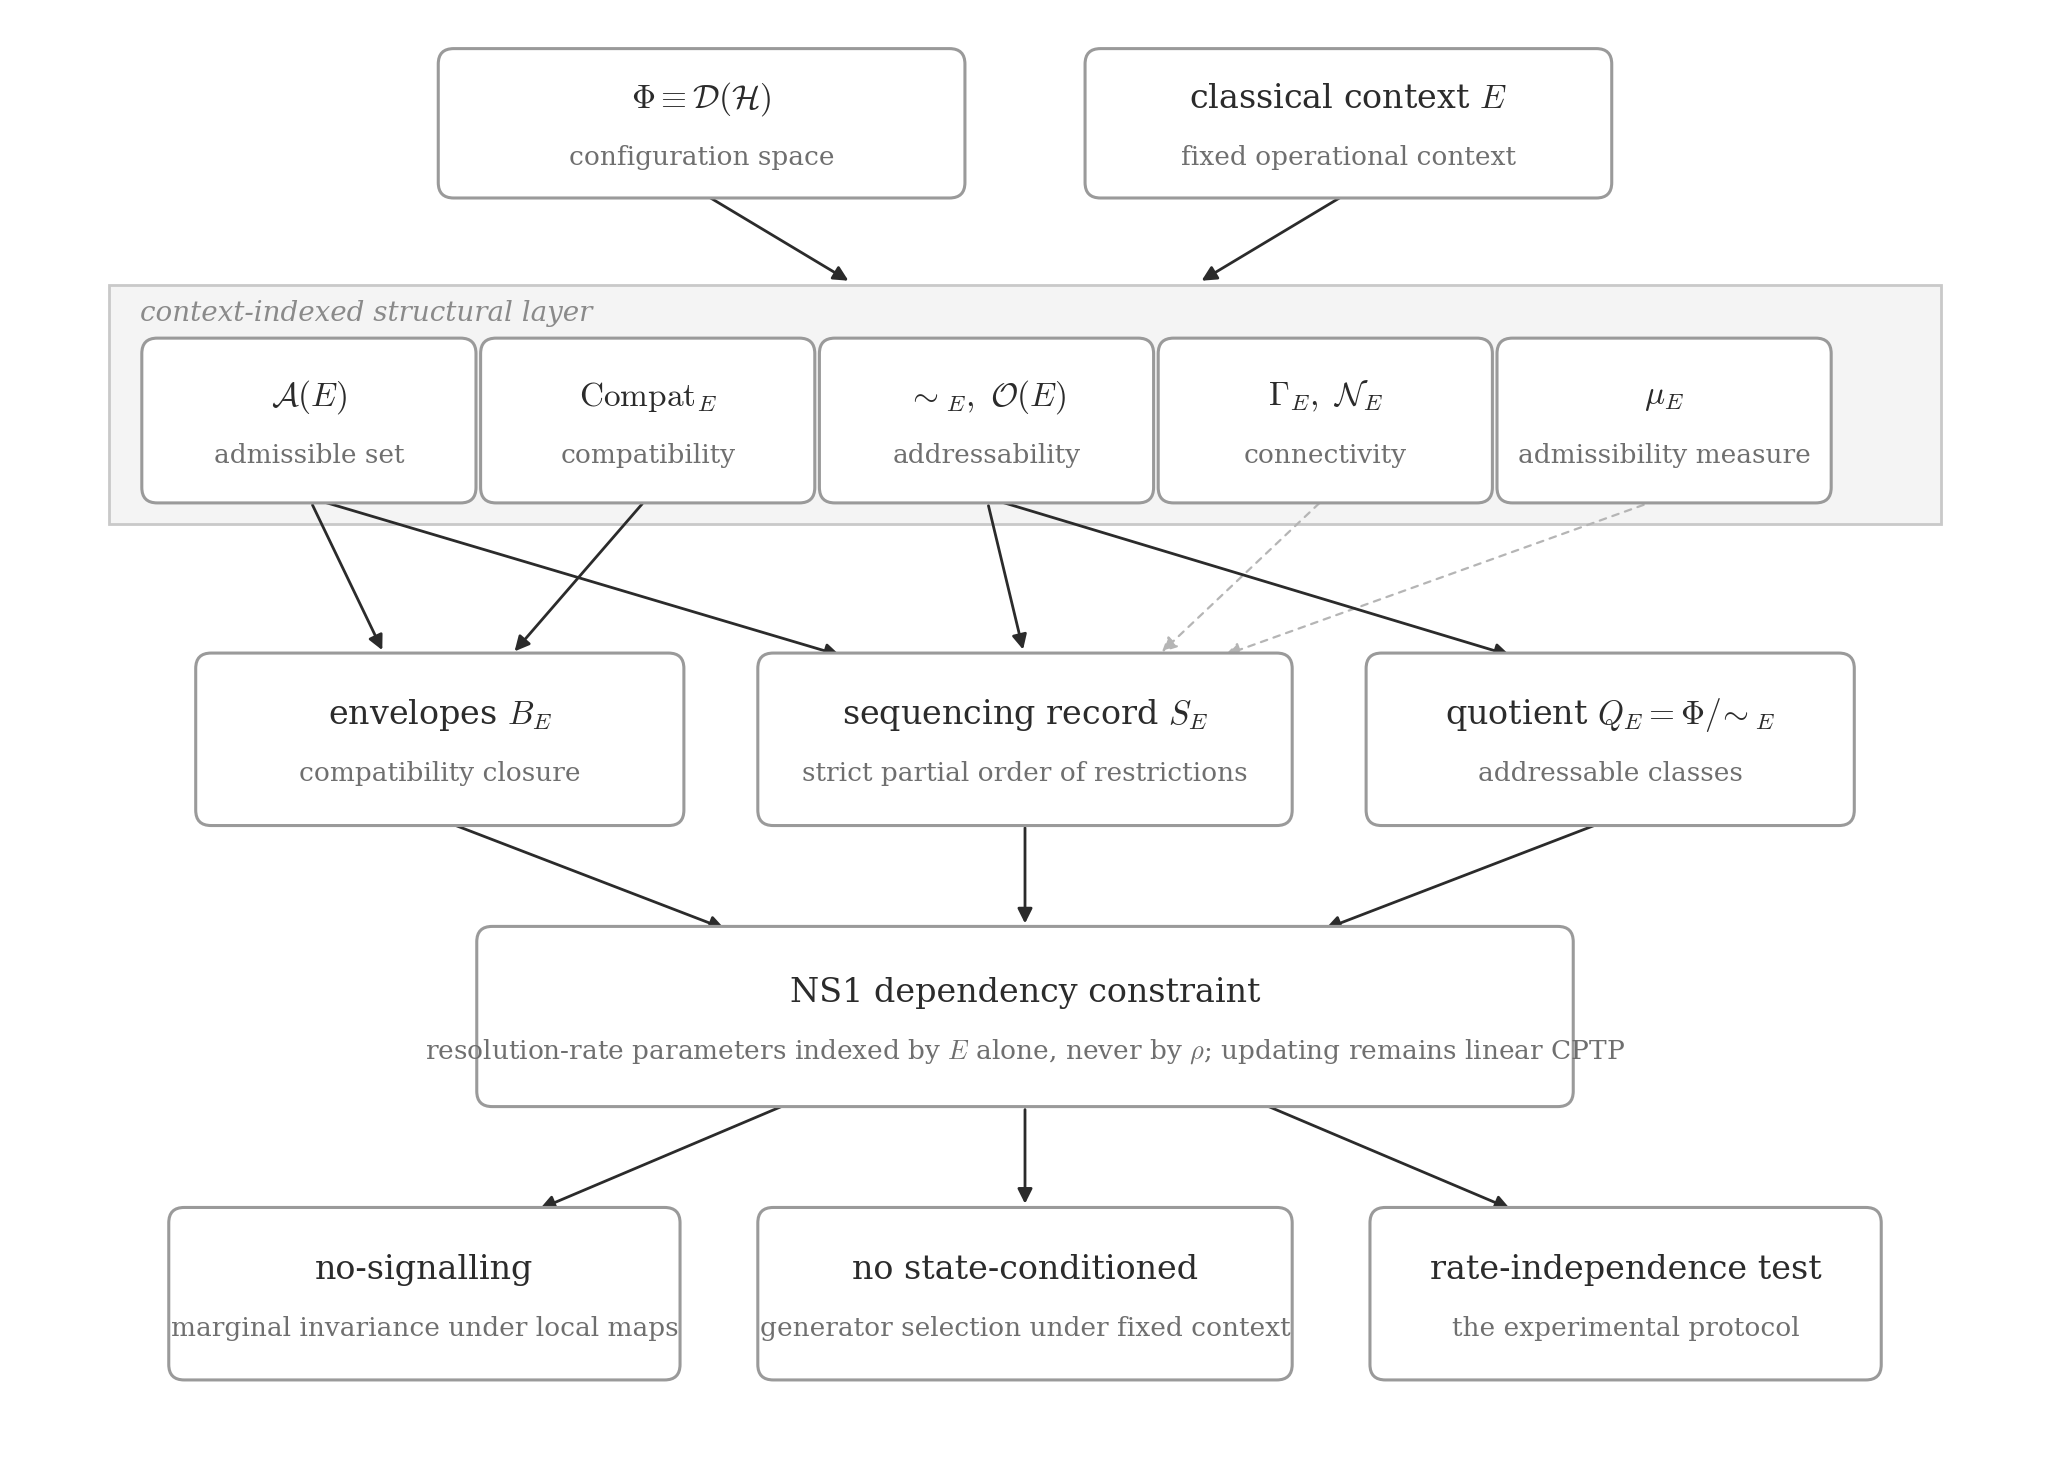
\includegraphics[width=0.98\linewidth]{fig_dependency_diagram.png}
\captionsetup{justification=raggedright,singlelinecheck=false}
\caption{\textbf{Dependency structure of the framework.} Primitives
(\(\Phi\) and the classical context \(E\)) feed the context-indexed
structural layer; the structural layer supports the derived
organization (compatibility envelopes, the sequencing record, the
addressability quotient); the NS1 dependency constraint governs
admissible updating over that structure; and its consequences include
no-signalling, the exclusion of state-conditioned generator selection,
and the rate-independence test of
Sec.~\ref{subsec:resolution_scaling_hypothesis}. Arrows denote
definitional or constraint dependence only, not dynamics, causation, or
temporal order; faint arrows indicate declared structural data entering
the sequencing record.}
\label{fig:dependency_diagram}
\end{figure}

\section*{Primitives and Symbols}

\paragraph{Purpose.}
This page fixes the complete set of foundational objects used in the
framework and the canonical meaning of each recurring symbol. All other
quantities are derived, representational, diagnostic, or bookkeeping
only.

\paragraph{Non-primitive reconstruction targets.}
SSAF does not take clock time, metric space, spacetime curvature,
force, or gravity as primitive objects. These quantities are treated as
reconstruction targets or phenomenological descriptors that may be
introduced only after the admissibility, compatibility, addressability,
connectivity, neighbourhood, measure, and sequencing structure has been
specified. In particular, any appearance of a time parameter, spatial
distance, geometric basin, potential, force, or gravity-like behavior in
later sections is representational unless explicitly derived from the
fixed primitive structure below. The framework therefore does not assume
gravity, time, metric geometry, or physical space at the foundation; it
asks what admissibility, connectivity, ordering, and reconstruction
structure must already be present for time-like and geometry-like
descriptions to be licensed.

\paragraph{Canonical primitives.}
\begin{itemize}

\item $\mathcal{H}$: Hilbert space of the model.
No physical claims are made at the level of $\mathcal{H}$ alone.

\item $\Phi$: configuration space,
\[
\Phi := D(\mathcal{H}),
\]
the set of density operators on $\mathcal{H}$ (positive,
trace-class, unit trace).
All predicates, relations, and maps in the framework act on $\Phi$.

\item $E$: classical context.
The complete specification of environmental and operational background
held fixed when making in-domain claims.
Formally,
\[
E \in \mathcal{E},
\]
where $\mathcal{E}$ is the context index set.
Changing $E$ changes the indexed description and never represents an
internal operation within a fixed-context analysis.

\item $\mathcal{A}(E)$: admissible domain under fixed context $E$,
\[
\mathcal{A}(E)\subseteq\Phi.
\]
$\mathcal{A}(E)$ specifies which configurations are admitted under the
fixed context $E$.
Admissibility specifies membership only. It does not by itself specify
compatibility, connectivity, neighbourhood structure, measure,
sequencing, or dynamical evolution.

\item $\mathcal{O}(E)$: observational interface under fixed context $E$,
\[
\mathcal{O}(E)\subseteq\mathcal{B}(\mathcal{H}).
\]
$\mathcal{O}(E)$ specifies the effect vocabulary available for
addressability and reconstruction tasks.

\item $\sim_E$: addressability relation under fixed context $E$,
\[
\rho\sim_E\sigma
\Longleftrightarrow
\forall M\in\mathcal{O}(E):
\mathrm{Tr}(M\rho)=\mathrm{Tr}(M\sigma).
\]
Configurations related by $\sim_E$ are operationally
indistinguishable through the interface $\mathcal{O}(E)$.

\item $\mathrm{Compat}_E$: compatibility predicate under fixed context
$E$,
\[
\mathrm{Compat}_E:
\mathcal{A}(E)\times\mathcal{A}(E)
\rightarrow
\{0,1\}.
\]
Compatibility is a pairwise licensing predicate only.
It determines whether two admissible configurations may coexist within
a common admissible structure.
The role boundaries for the objects in this list are stated once in
Sec.~\ref{sec:separation_discipline}.

\item $\Gamma_E$: connectivity structure under fixed context $E$,
\[
\Gamma_E := (\mathcal{A}(E),\mathcal{R}_E),
\]
where
\[
\mathcal{R}_E
\subseteq
\mathcal{A}(E)\times\mathcal{A}(E)
\]
is a context-indexed connectivity relation.
$\Gamma_E$ records the global organization of admissible structure.
\item $\mathcal{N}_E$: neighbourhood structure under fixed context $E$,
\[
\mathcal{N}_E:
\mathcal{A}(E)
\rightarrow
\mathcal{P}(\mathcal{A}(E)).
\]
For each admissible configuration $\rho$,
\[
\mathcal{N}_E(\rho)
\subseteq
\mathcal{A}(E)
\]
denotes the neighbourhood associated with $\rho$.
$\mathcal{N}_E$ is derived from the connectivity structure, with
$\mathcal{N}_E(\rho)=\{\sigma\in\mathcal{A}(E):(\rho,\sigma)\in\mathcal{R}_E\}$.
It provides local relatedness within the admissible domain and carries
no information beyond $\Gamma_E$. No metric notion of distance is
assumed.

\item $\mu_E$: admissibility measure under fixed context $E$,
\[
\mu_E:
\mathcal{P}(\mathcal{A}(E))
\rightarrow
[0,\infty].
\]
$\mu_E$ assigns structural weight to admissible regions.
Concentration, density, dispersion, relative size and occupancy are
derived comparisons built from it, not separate primitives.
It is assumed monotone on admissible regions:
\[
U\subseteq V\subseteq \mathcal{A}(E)
\quad\Longrightarrow\quad
\mu_E(U)\leq \mu_E(V).
\]
$\mu_E$ is not a probability measure and does not determine admissible
updates, map selection, generators, or resolution rates.

\item $\mathrm{Coh}_E(\rho)$: coherence functional under fixed context
$E$.
A diagnostic functional on $\Phi$ used only for classification,
comparison, and description relative to $E$.
$\mathrm{Coh}_E$ never appears in admissibility rules, update-family
selection, generators, or rate data.

\end{itemize}

\paragraph{Representational maps and auxiliary symbols.}

\begin{itemize}

\item $\Lambda_{E,\Delta}$: admissible updating map (representation
only), a linear CPTP map indexed only by fixed context $E$ and an
explicit bookkeeping label $\Delta \ge 0$,
\begin{equation}
\Lambda_{E,\Delta} : \Phi \to \Phi.
\end{equation}
The label $\Delta$ carries no ontological meaning and is not a
fundamental time parameter; it is used only when updates are
represented.

\item $\tau$: sequencing label or abstract ordering index. $\tau$
carries no metric or temporal meaning and is used only to represent
admissible ordering structure.

\item $t$: reconstructed operational clock parameter,
\begin{equation}
t = \mathcal{R}(\tau;E),
\end{equation}
introduced only at the representational level. $t$ is not a primitive
parameter of the framework and does not enter admissibility,
compatibility, connectivity, neighbourhood structure, measure, or
update-family selection.

\item $\mathcal{M}(E)$: context-indexed core set or designated sector
used in model-specific basin-style constructions,
\begin{equation}
\mathcal{M}(E) \subseteq \mathcal{A}(E) \subseteq \Phi,
\end{equation}
when the construction is intended to be admissibility-restricted.
It is introduced only where explicitly stated and is not assumed
primitive to the full framework unless declared as such in a
model-specific construction.

\end{itemize}

\paragraph{Dependency discipline (NS1).}
All admissible updating and resolution-rate data are functions of the
fixed classical context $E$ only and never of the quantum state:
\begin{equation}
\lambda_\alpha = F_\alpha(E),
\qquad
\frac{\delta \lambda_\alpha}{\delta \rho} = 0.
\end{equation}
Here $\lambda_\alpha$ denotes representational rate parameters used for
bookkeeping when updates are modeled. Admissible in-domain updating is
represented, when represented, by linear CPTP maps indexed only by $E$
and any explicit bookkeeping labels.

\paragraph{Quantifier discipline (standing rule).}
Unless explicitly stated otherwise:
\begin{itemize}
\item $E$ is fixed throughout a claim, lemma, or proof.
\item $\rho, \sigma \in \Phi$ denote arbitrary configurations;
admissibility is written explicitly as
$\rho \in \mathcal{A}(E)$ when required.
\item Any map written $\mathcal{T}^E$ denotes a CPTP map
$\mathcal{T}^E : \Phi \to \Phi$ used under that same fixed context $E$.
\end{itemize}

\paragraph{Derived and bookkeeping symbols (not primitive).}
\begin{itemize}

\item $\mathcal{E}_E(\rho_0)$: compatibility envelope generated from a
seed configuration $\rho_0$ under fixed $E$ using
$\mathrm{Compat}_E$, defined only where introduced. Since
$\mathrm{Compat}_E$ is a pairwise coexistence predicate, this envelope
does not by itself define connectivity, neighbourhood structure, or
measure.

\item $\delta_E^{\mathrm{ord}}(W)$: ordering-density diagnostic over a
finite sequencing window $W$ under fixed context $E$. This quantity
measures the average admissible-set restriction across the chosen
window when a realized sequencing record is represented by a nested
admissible-set chain. It is derived from $\mu_E$ and the declared
restriction chain; it is not primitive, not a time density, not a
dynamical rate, and does not modify $\mathcal{A}(E)$,
$\mathrm{Compat}_E$, $\Gamma_E$, $\mathcal{N}_E$, $\mu_E$, or any
NS1-licensed update data.

\item \textbf{Addressable envelope (interface-bounded):} a derived
restriction $\mathcal{E}(E) \subseteq \mathcal{A}(E)$ on which the
interface $\mathcal{O}(E)$ and the induced relation $\sim_E$ support
the intended task, such as identification, reconstruction, or protocol
continuation. No claim is made that
$\mathcal{E}(E) = \mathcal{A}(E)$ is possible in general.

\item \textbf{Inherent boundary (envelope non-closure):} a
domain-of-definition failure in which an intended continuation or step
relation, toy- or protocol-defined under fixed $E$, has no licensed
successor within the addressable envelope. In such cases, comparisons
are \emph{undefined} rather than unknown; no prohibition, firewall, or
ontological edge is implied.

\item $\mathrm{Obs}_E$: observational interface map,
\[
\mathrm{Obs}_E : \mathcal{A}(E) \to \mathcal{O}_E,
\]
sending configurations to interface reports. It induces $\sim_E$ via
\[
\rho \sim_E \sigma
\Leftrightarrow
\mathrm{Obs}_E(\rho) = \mathrm{Obs}_E(\sigma).
\]

\item $\mathrm{Rec}_E$: reconstruction map,
\[
\mathrm{Rec}_E :
\mathrm{Obs}_E(\mathcal{E}(E))
\to
\mathcal{E}(E),
\]
defined only on domains where the interface supports unique
identification. It is post-ordering bookkeeping only and does not
modify admissibility.

\item $\mathrm{Next}_E$: continuation relation,
\[
\mathrm{Next}_E :
\mathcal{A}(E)
\rightrightarrows
\mathcal{A}(E),
\]
a set-valued bookkeeping map specifying which configurations remain
admissible after an externally specified protocol step. No dynamical
meaning is implied.

\item $Q_E := \Phi/{\sim_E}$: addressability quotient, the set of
equivalence classes under $\sim_E$. Used in figures and quotient
constructions only.

\item $\mathrm{Sep}_E(A{:}B)$: $E$-admissible separable hull,
\[
\mathrm{Sep}_E(A{:}B)
:=
\mathrm{conv}\{
\rho_A \otimes \rho_B :
\rho_A \in \mathcal{A}_A(E),\,
\rho_B \in \mathcal{A}_B(E)
\}.
\]
Used to define factorizability of joint admissibility.

\item $\mathcal{E}^{\mathrm{pair}}_E$: compatible pair set,
\[
\mathcal{E}^{\mathrm{pair}}_E :=
\{
(\rho,\sigma)
\in
\mathcal{A}(E)\times\mathcal{A}(E) :
\mathrm{Compat}_E(\rho,\sigma)=1
\}.
\]
Bookkeeping object for compatibility tests in toy models. This is a
pairwise coexistence object and must not be read as a neighbourhood,
connectivity graph, or measure.

\item $\mu_{E,\rho}$: Born-weight measure, a positive normalized set
function on the $\sigma$-algebra generated by resolution classes
$\{R_k(E)\}_k$ under fixed $E$ and configuration $\rho$.
Representational only; does not parameterize NS1-licensed update
families. This object is distinct from the structural admissibility
measure $\mu_E$.

\item $(\mathrm{IC}_E)$: interface-closure condition, the standing
assumption that admissible in-domain CPTP maps preserve
$\mathcal{O}(E)$ under the Heisenberg dual. Invoked explicitly wherever
stated; not assumed globally.

\item $B(E)$: basin sector, a positively invariant subset
\[
B(E) \subseteq \mathcal{A}(E)
\]
under admissible updating. Used in coherence-basin constructions and
spin-class definitions. Introduced only where explicitly declared and
not treated as a primitive geometric object.

\item $\mathcal{L}_E(B)$: admissible loop family, a stipulated or
derived family of loop representatives in a declared basin or
circulation-supporting sector $B$, equipped where needed with
concatenation and inversion. Used in spin-class and
circulation-witness constructions. It is not a primitive of the full
framework and must not be confused with the connectivity primitive
$\Gamma_E$.

\item ${\sim}^{\mathrm{spin}}_E$: spin-class equivalence, defined by
equality of a chosen circulation witness $W_E$ on a basin sector
$B(E)$. Representational and diagnostic only.

\item $\Theta(\rho_n)$: cumulative ordering diagnostic, a monotone
scalar defined along an admissible ordering chain via coherence
functional differences. Bookkeeping only; does not parameterize
admissibility or NS1-licensed update data.

\item $W_E \subset S^1$: phase-offset acceptance window, toy-level
descriptor only. A bookkeeping subset of the phase circle used in
finite-witness toys to encode which phase offsets are treated as
accepted within that toy. $W_E$ is not an envelope in $\Phi$, does not
modify $\mathcal{A}(E)$ or $\mathrm{Compat}_E$, and must not be read as
introducing a second envelope notion.

\item $t = \mathcal{R}(\tau; E)$: reconstructed time-coordinate,
representation only, defined only when a reconstruction dictionary is
invoked.

\item $\delta(\tau)$: articulation density, or granularity, of a
reconstruction at label $\tau$. Undefined outside a reconstruction
scheme; carries no physical or dynamical meaning.

\item $\{U^{(k)}_E\}_{k \in K}$: finite family of unary
constraint-sets under fixed context $E$,
\[
U^{(k)}_E \subseteq \mathcal{A}(E) \subseteq \Phi.
\]
Each $U^{(k)}_E$ is used only for membership tests in profile
construction and introduces no updating rules, dynamics, or
state-dependent dependence.

\item $K$: finite index set labeling the unary constraint vocabulary
used to define signature or profile classes. $K$ carries no ordering
or metric structure.

\item $\mathbf{s}_E : \mathcal{A}(E) \to \{0,1\}^K$:
constraint-membership profile map, defined by
\[
\mathbf{s}_E(\rho)_k :=
\mathbf{1}\{\rho \in U^{(k)}_E\}.
\]
Used only for classification and structural ordering.

\item $\equiv_E$: profile-equivalence relation on
$\mathcal{A}(E)$ induced by $\mathbf{s}_E$, used to define signature
classes.

\item $\mathcal{S}_{\mathbf{s}}(E)$: signature class, or equivalence
class, in $\mathcal{A}(E)$ associated to signature vector
$\mathbf{s} \in \{0,1\}^K$.

\item $\preceq$: coordinatewise partial order on $\{0,1\}^K$ and its
induced order on signature classes. Structural only; introduces no
sequencing or dynamics.

\item $\mathcal{A}_K(E)$: constraint-refined admissible domain,
optional,
\[
\mathcal{A}_K(E)
:=
\mathcal{A}(E)
\cap
\bigcap_{k \in K} U^{(k)}_E,
\]
a representational restriction of the comparison domain.

\item $\mathcal{K}_j(E)$: compatibility class, or maximal pairwise
compatible sector, under fixed $E$, i.e.\ a maximal-by-inclusion subset
$\mathcal{K} \subseteq \mathcal{A}(E)$ such that
\[
\mathrm{Compat}_E(\rho,\sigma)=1
\]
for all distinct $\rho, \sigma \in \mathcal{K}$. This is a
compatibility object only; it is not necessarily a connected component
of $\Gamma_E$ and does not define a neighbourhood or measure.

\end{itemize}

\paragraph{Composite-system conventions (factorization invoked
explicitly).}
When a bipartite or multipartite structure is used in a toy or example,
we assume an explicitly chosen representational factorization of
$\mathcal{H}$,
\[
\mathcal{H} = \mathcal{H}_A \otimes \mathcal{H}_B
\quad(\text{or } \mathcal{H} = \bigotimes_i \mathcal{H}_i).
\]
This introduces no new primitives; it is a representational
decomposition used only where stated. The induced configuration spaces
are
\[
\Phi_{AB} := D(\mathcal{H}_A \otimes \mathcal{H}_B), \qquad
\Phi_A := D(\mathcal{H}_A), \qquad
\Phi_B := D(\mathcal{H}_B).
\]
Partial traces are the standard CPTP marginalization maps
\[
\mathrm{Tr}_B : \Phi_{AB} \to \Phi_A, \qquad
\mathrm{Tr}_A : \Phi_{AB} \to \Phi_B.
\]
Where needed, a context-indexed jointly admissible sector is written
\[
\mathcal{A}_{AB}(E) \subseteq \Phi_{AB},
\]
and the induced marginal admissible sets are its partial-trace images
\[
\mathcal{A}_A(E) := \{\mathrm{Tr}_B(\rho_{AB}) :
\rho_{AB} \in \mathcal{A}_{AB}(E)\}, \qquad
\mathcal{A}_B(E) := \{\mathrm{Tr}_A(\rho_{AB}) :
\rho_{AB} \in \mathcal{A}_{AB}(E)\}.
\]
All dependence remains indexed only by $E$ under NS1; no auxiliary
control variables are introduced by factorization notation.

\section{Core Definitions and Ontological Commitments}
\label{sec:core_definitions}

This section fixes the primitive objects and structural relations used
throughout SSAF. The definitions here are \emph{structural}:
context-indexed, model-agnostic, and free of dynamical assumptions.
They specify the domains on which later constructions act and the
predicates and structural objects later sections will use. No additional
substrate, mechanism, or dynamical generator is introduced here.
Any geometric, operational, connectivity, neighbourhood, measure, or
reconstruction structure is introduced explicitly and remains
context-indexed.

\subsection{Primitive Objects and Structural Predicates}
\label{subsec:core_defs_objects}

\paragraph{Hilbert space and state space.}
Let $\mathcal{H}$ be a complex separable Hilbert space. Physical
configurations are represented by density operators
\[
\mathcal{D}(\mathcal{H}) :=
\bigl\{\rho \in \mathcal{T}_1(\mathcal{H})
: \rho = \rho^\dagger,\ \rho \succeq 0,\ \mathrm{Tr}(\rho)=1
\bigr\},
\]
where $\mathcal{T}_1(\mathcal{H})$ denotes the trace-class operators on
$\mathcal{H}$~\cite{Watrous2018}. SSAF takes the configuration space to be
\begin{equation}
\Phi := \mathcal{D}(\mathcal{H}).
\label{eq:phi_def}
\end{equation}

Pure-state descriptions are recovered as the rank-$1$ subset
\[
\rho = |\psi\rangle\langle\psi|,
\]
equivalently rays in projective space $\mathbb{P}(\mathcal{H})$, used
only as a standard chart for pure-state arguments and not as a
replacement for $\Phi$ as the ambient state
space~\cite{Watrous2018,NielsenChuang2010}.

No metric, locality, embedding, topology, connectivity, neighbourhood
assignment, measure, sequencing relation, or dynamical flow is assumed
on bare $\Phi$ at this stage. Such structure is introduced only after a
fixed classical context $E$ and admissible domain $\mathcal A(E)$ have
been specified. In particular, $\Gamma_E$, $\mathcal N_E$, and $\mu_E$
are context-indexed structural objects over admissible structure, not
background structure on $\Phi$ itself.

\paragraph{Notation and conventions.}
Symbols and primitives follow the conventions fixed in the Primitives and
Symbols section. In particular, $\Phi := \mathcal{D}(\mathcal{H})$
throughout, and $E$ denotes the fixed classical context. All
admissibility, compatibility, connectivity, neighbourhood, measure, and
ordering statements are context-indexed structures over $\Phi$ or over
admissible domains within $\Phi$, as specified below.

\paragraph{Classical context.}
A \emph{classical context} $E$ is an element of an index set
$\mathcal{E}$ whose members parameterize admissibility, compatibility,
connectivity, neighbourhood structure, admissibility measure, and
reconstruction structure. $E$ encodes the complete specification of
classical and environmental descriptors, boundary conditions, coupling
profiles, apparatus settings, coarse-graining choices, and any
explicitly specified external controls, held fixed when making
in-domain claims. Two properties follow directly from this definition.

First, $E$ is not a dynamical variable. Changing $E$ corresponds to
adopting a different indexed description, not performing an operation
internal to a fixed-context analysis. No admissible in-domain map under
fixed $E$ can modify $E$ itself.

Second, $E$ is not a quantum object. It encodes classical descriptors
only and never depends on the quantum state $\rho$, any decomposition
of $\rho$, or any state-derived diagnostic. This is the formal ground
of the NS1 constraint: since $E$ is classical and state-independent by
definition, any resolution-rate parameter
$\lambda_\alpha = F_\alpha(E)$ is automatically state-independent.

\paragraph{Relationship between $\mathcal{A}(E)$,
$\mathrm{Compat}_E$, and the structural layer.}
The admissible set $\mathcal{A}(E)$, compatibility predicate
$\mathrm{Compat}_E$, connectivity structure $\Gamma_E$, neighbourhood
assignment $\mathcal{N}_E$, and admissibility measure $\mu_E$ are all
indexed by the same fixed classical context $E$, but they perform
different structural roles.

The admissible set
\[
\mathcal{A}(E)\subseteq\Phi
\]
specifies membership only. It determines which configurations are
admitted under fixed context $E$. It does not, by itself, determine
pairwise compatibility, connectivity, neighbourhood structure, measure,
sequencing, or dynamics.

The compatibility predicate
\[
\mathrm{Compat}_E:
\mathcal{A}(E)\times\mathcal{A}(E)
\to
\{0,1\}
\]
is a pairwise coexistence predicate. It licenses whether two admissible
configurations may co-occur within a common admissible structure. It
does not, by itself, define a neighbourhood, connected component,
topology, basin, or measure.

The connectivity structure
\[
\Gamma_E=(\mathcal{A}(E),\mathcal{R}_E)
\]
records global organization over the admissible domain. The
neighbourhood assignment $\mathcal{N}_E$ records local relatedness, and
the admissibility measure $\mu_E$ records structural weight or
concentration of admissible regions. These objects are distinct from
both admissibility and compatibility unless a model-specific
construction explicitly derives one from another.

Consequently, no global non-isolation requirement is imposed on
$\mathcal{A}(E)$. A singleton admissible domain, terminal configuration,
or degenerate admissible sector is allowed unless explicitly excluded by
a model-specific nondegeneracy condition. When a construction requires
every admitted configuration to participate in at least one
compatibility relation, that assumption must be stated locally, for
example as
\begin{equation}
\forall\, \rho \in \mathcal{A}(E),\quad
\exists\, \sigma \in \mathcal{A}(E),\; \sigma \neq \rho,\quad
\mathrm{Compat}_E(\rho, \sigma) = 1.
\label{eq:admissibility_compatibility_nondegeneracy}
\end{equation}
Equation~\eqref{eq:admissibility_compatibility_nondegeneracy} is
therefore a model-specific nondegeneracy condition, not a standing
definition of admissibility.

No symmetry, transitivity, reflexivity, connectedness, metric
structure, or topological structure is assumed for
$\mathrm{Compat}_E$, $\Gamma_E$, or $\mathcal{N}_E$ unless explicitly
introduced in the model under discussion.

\subsection{Admissibility, Compatibility, and Addressability}
\label{subsec:admissibility_commitment}

\begin{definition}[Admissibility and the admissible set]
\label{def:admissibility}
Admissibility is a primitive structural predicate indexed by a fixed
classical context \(E\). For each \(E\) it determines the
\emph{admissible set}
\[
\mathcal{A}(E) \subseteq \Phi,
\]
the domain of configurations admitted by the \(E\)-indexed description.
A configuration \(\rho \in \mathcal{A}(E)\) is \emph{admissible under}
\(E\); a configuration in \(\Phi \setminus \mathcal{A}(E)\) remains an
element of \(\Phi\) but lies outside the in-domain claim set of any
description or protocol constrained to \(E\): it is not licensed as a
target of inference, continuation, reconstruction, or addressability
within that context. Admissibility specifies contextual membership
only; it does not by itself assign the compatibility, connectivity,
neighbourhood, measure, or addressability structure defined separately
below. Sequencing is introduced in later sections as a realized
restriction record within admissible structure.
\end{definition}

\begin{remark}[What admissibility is not]
\label{rem:admissibility_exclusions}
Admissibility is operational-structural, not ontological, and three
readings are explicitly excluded. It is not \emph{ontological
availability}: it does not say which configurations exist, and the
complement \(\Phi \setminus \mathcal{A}(E)\) is not metaphysically
absent. It is not \emph{epistemic uncertainty}: it does not track any
agent's knowledge or ignorance, since \(E\) is fixed by the physical and
operational arrangement rather than by what anyone knows. It is not
\emph{bare logical consistency}: it is indexed to a physical context,
not to formal coherence alone. Where later sections call a configuration
``unavailable'' or ``ruled out'' under \(E\), this is shorthand for
exclusion from the admissible in-domain description under that fixed
context and carries no ontological commitment.
\end{remark}

\begin{remark}[Admissibility versus addressability]
\label{rem:admissibility_vs_addressability}
Admissibility is distinct from addressability. The observational
interface \(\mathcal{O}(E)\) determines which distinctions can be drawn
through trace-pairing expressions \(\mathrm{Tr}(M\rho)\),
\(M \in \mathcal{O}(E)\), and thereby induces the addressability
relation \(\sim_E\). By contrast, \(\mathcal{A}(E)\) specifies the
domain on which such operational questions are licensed at all.
Addressability refines operational distinguishability \emph{within} an
admissible context; it does not define admissibility itself unless a
model-specific construction explicitly imposes that identification.
\end{remark}

\paragraph{Structural roles assigned separately.}
Admissibility specifies membership only. It does not by itself specify
compatibility, connectivity, neighbourhood structure, measure,
sequencing, or dynamical evolution. Those structures are supplied, when
needed, by \(\mathrm{Compat}_E\), \(\Gamma_E\), \(\mathcal N_E\),
\(\mu_E\), and the sequencing relation.

\paragraph{Compatibility predicate.}
Within fixed \(E\), compatibility is a primitive, context-indexed
binary predicate on the admissible domain,
\begin{equation}
\mathrm{Compat}_E :
\mathcal A(E)\times \mathcal A(E)
\to
\{0,1\},
\qquad
\mathrm{Compat}_E(\rho,\sigma)=1
\;\Longleftrightarrow\;
\text{\(\rho\) and \(\sigma\) are compatible under \(E\).}
\label{eq:compat_def}
\end{equation}
Compatibility is a pairwise coexistence predicate only. It does not by
itself define connectivity, neighbourhood structure, measure, topology,
basin structure, sequencing, or dynamics.

No symmetry, transitivity, reflexivity, metric, or topological
structure is assumed unless explicitly introduced within a stated
model. \(\mathrm{Compat}_E\) is indexed only by the fixed context \(E\)
and is independent of the quantum state, diagnostic quantities
including coherence, and any realized restriction record, in accordance
with NS1~\cite{Kraus1983,NielsenChuang2010,Watrous2018,Gisin1989,Gisin1990,
Polchinski1991}.

\paragraph{Compatibility envelopes.}
An \emph{envelope} under \(E\) is a subset
\[
S\subseteq \mathcal A(E)
\]
closed under pairwise compatibility:
\begin{equation}
S\ \text{is an envelope}
\;\Longleftrightarrow\;
\forall\,\rho,\sigma\in S,\quad
\mathrm{Compat}_E(\rho,\sigma)=1.
\label{eq:envelope_def}
\end{equation}
Envelopes may be taken as maximal by inclusion; maximality is not
assumed unless stated.

An envelope is a compatibility object. It is not automatically a
connected component of \(\Gamma_E\), a neighbourhood under
\(\mathcal N_E\), a basin, or a measured region under \(\mu_E\), unless
a model-specific construction explicitly identifies those structures.

\paragraph{Observational interface and addressability.}
Admissibility specifies which configurations are admitted by the
\(E\)-indexed description. Separately, an observational interface
specifies which distinctions among admissible configurations are
addressable by records.

Let
\[
\mathrm{Eff}(\mathcal H)
:=
\{M\in\mathcal B(\mathcal H):0\preceq M\preceq I\}
\]
denote the effect operators on \(\mathcal H\). Let
\(\mathcal O(E)\subseteq \mathrm{Eff}(\mathcal H)\) be a fixed set of
admissible diagnostic effects under context
\(E\)~\cite{NielsenChuang2010,Watrous2018}. Define the
\(E\)-dependent addressability relation \(\sim_E\) on \(\Phi\) by
\begin{equation}
\rho\sim_E\sigma
\;\Longleftrightarrow\;
\mathrm{Tr}(M\rho)=\mathrm{Tr}(M\sigma)
\quad
\text{for all }M\in\mathcal O(E).
\label{eq:addressability_relation}
\end{equation}

The quotient
\[
\mathcal A(E)/{\sim_E}
\]
is the \emph{addressable admissible} configuration space under \(E\):
admissible configurations in the same equivalence class are
operationally indistinguishable by \(\mathcal O(E)\), even if they are
distinct elements of \(\Phi\).

\begin{figure}[t]
\centering
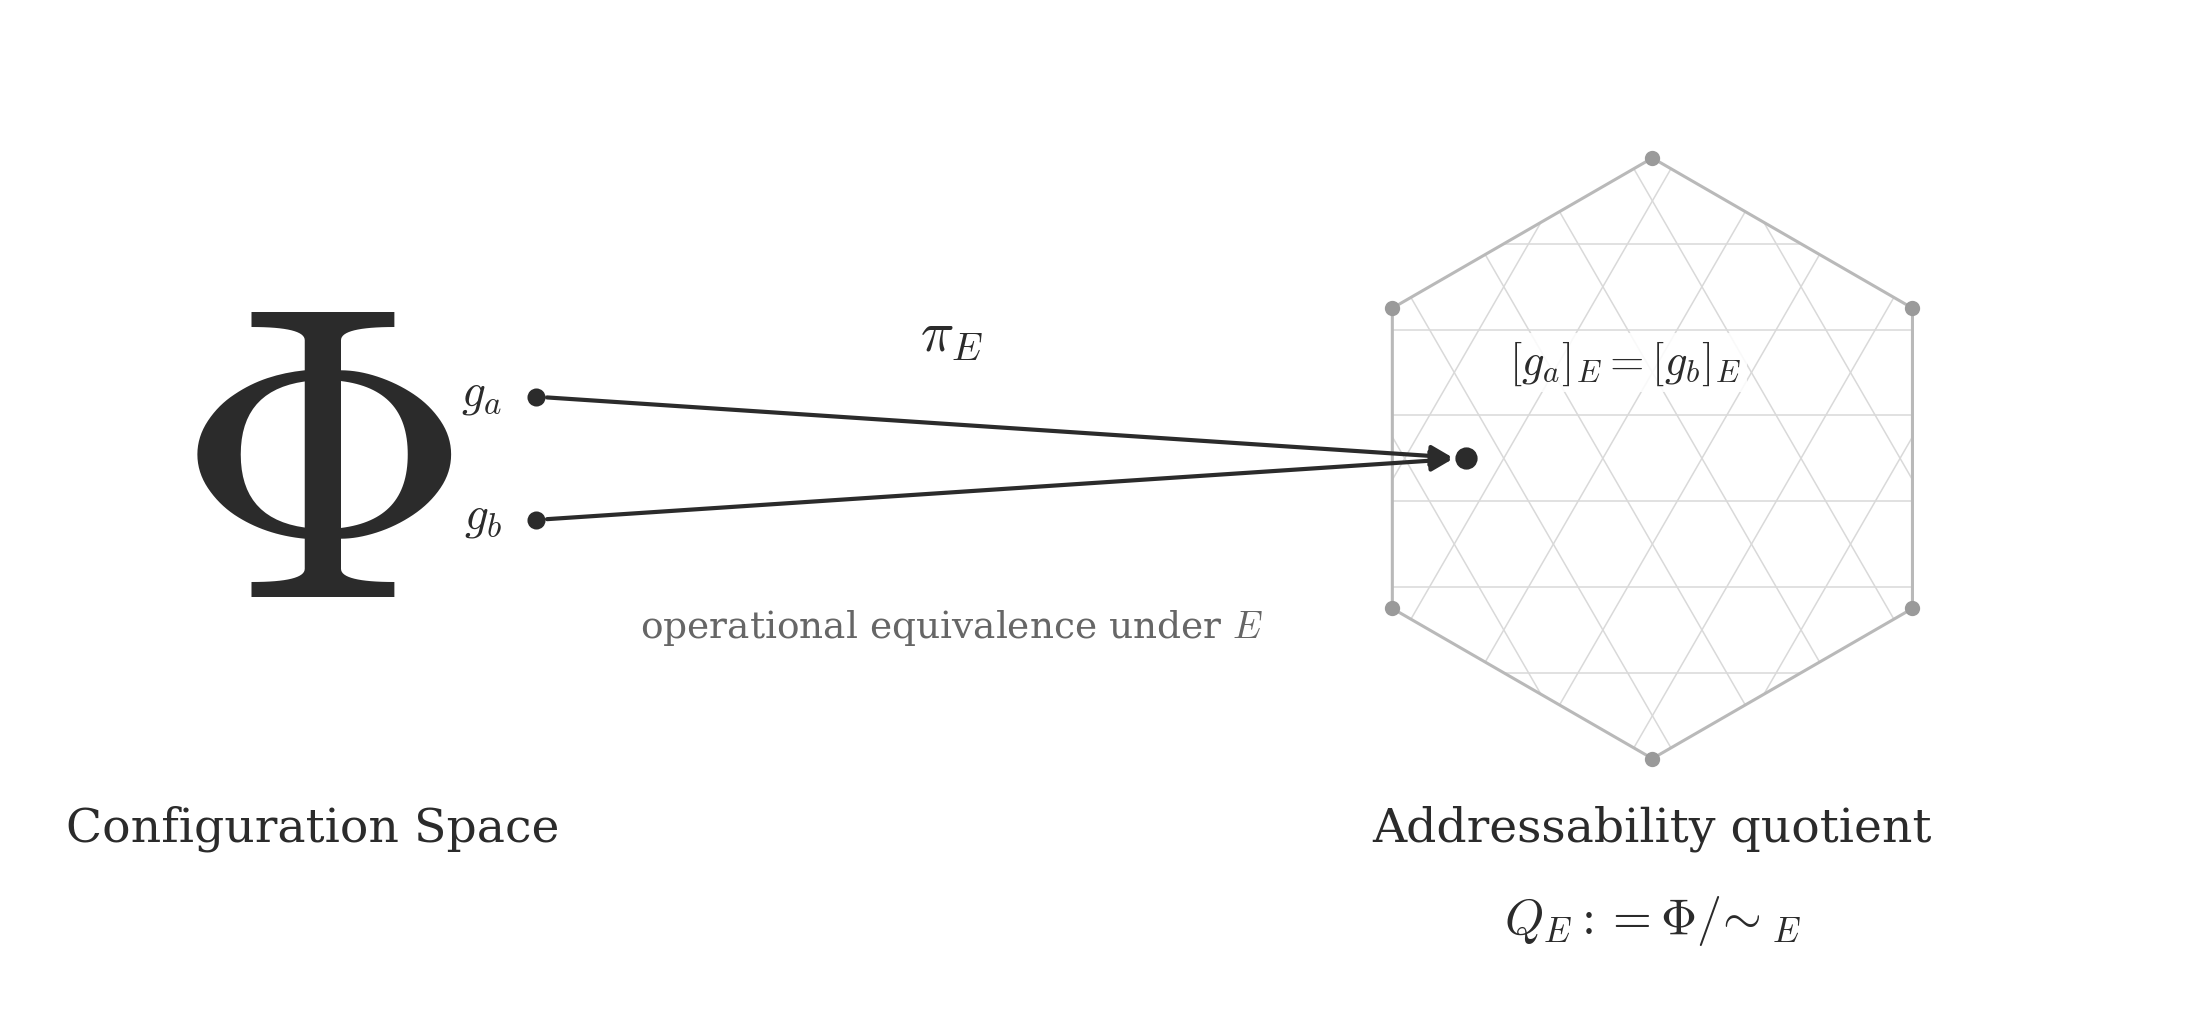
\includegraphics[width=0.72\linewidth]{addressibility.png}
\captionsetup{justification=raggedright,singlelinecheck=false}
\caption{
Addressability as equivalence-class projection from configuration space
\(\Phi\) to the addressability quotient \(Q_E := \Phi/\!\sim_E\) under
fixed classical context \(E\). Points \(g_a,g_b\in\Phi\) denote distinct
configurations that are operationally indistinguishable at the interface:
\(g_a\neq g_b\) in \(\Phi\) but \(g_a\sim_E g_b\), so
\([g_a]_E=[g_b]_E\) in \(Q_E\). Multiple such configurations collapse
to a single addressable class under the projection
\(\pi_E:\Phi\to Q_E\). Arrows denote identification under \(\sim_E\),
not dynamics, transport, or information flow. The diagram captures the
central distinction of SSAF: difference in configuration space does not
imply difference in addressability, and admissible structure may exist
in \(\Phi\) while remaining operationally inaccessible under fixed \(E\).
}
\label{fig:addressability_quotient}
\end{figure}

\paragraph{Semantic rule.}
Representationally opposable outcomes do not by themselves imply
structural incompatibility. If multiple configurations remain pairwise
compatible under \(E\), the appropriate object of description is the
admissible family itself. Introducing selection prior to loss of
compatibility constitutes an outcome-conditioned restriction, which is
excluded by NS1.

For concreteness, one may take \(\mathcal O(E)\) to be the set of POVM
elements \(\{M_r(E)\}_{r\in\mathcal R}\), with
\(M_r(E)\succeq 0\) and
\[
\sum_{r\in\mathcal R}M_r(E)=I,
\]
where \(\mathcal R\) is an outcome index set. In that case
\[
p_E(r\mid\rho)=\mathrm{Tr}(M_r(E)\rho),
\]
and Eq.~\eqref{eq:addressability_relation} holds if and only if all
POVM outcome statistics agree.

\paragraph{Coarsening limits.}
In strongly constrained contexts, \(\sim_E\) may become coarse. In the
extreme, \(\sim_E\) may be trivial, meaning all configurations in the
domain under consideration belong to a single equivalence class. In
that case no nontrivial sequencing of addressably distinct
configurations is defined relative to \(\mathcal O(E)\). This is an
interface-induced domain-of-definition limit: the description lacks the
vocabulary to state finer distinctions.

\subsection{Admissibility and Phase Relationships}
\label{subsec:admissibility_phase_relationships}

SSAF expresses admissibility primarily through phase relationships. This
is a modeling commitment about the descriptor in which compatibility is
assessed, in the sense of Axiom~II, and not an ontological claim that
phase is a substance prior to the state space on which it is defined.
Within that commitment, the primary distinctions the framework reads are
relational rather than structural: oscillation, relative phase, and the
coherence relations among configurations, rather than objects,
locations, or geometric forms. The motivating intuition is the smallest
available case. A spin degree of freedom is already characterized by a
relative phase, and it is that relative phase, not any spatial picture of
the spin, that determines whether two such configurations remain
compatible under a fixed context. SSAF takes this as the template: where
a relative phase can be assigned, admissibility is assessed in terms of
it first, and any structural or geometric description is a reconstructed
account of the result.

Admissibility is the formal record of which phase relationships remain
jointly satisfiable. Configurations are admissible under a fixed context
\(E\) when the phase relationships that \(E\) requires can be
simultaneously maintained, and inadmissible when they cannot. The
admissible set \(\mathcal{A}(E)\) collects the configurations whose phase
relationships remain licensed by \(E\); the compatibility predicate
\(\mathrm{Compat}_E\) records which configurations can be co-addressed
within the same phase-admissible domain. In this reading, what the
framework treats as primary is the compatibility relation, and the
larger-scale structures, atomic, molecular, biological, astrophysical,
appear as reconstructions of admissible phase organization at their
respective scales rather than as the primitive basis of admissibility
itself.

Two cautions fix the scope of this reading and keep it consistent with
the rest of the paper. First, phase enters only through \(E\)-indexed
admissibility, compatibility, and the declared interface statistics
\(\mathrm{Tr}(M\rho)\) with \(M \in \mathcal{O}(E)\); no independent phase
space, canonical coordinates, or hidden phase substance is introduced as
primitive (Axiom~II). The claim is that phase relationships are the
\emph{descriptor of first resort}, not that they are metaphysically prior
to the operator substrate on which they are represented. Second, this
subsection states a representational stance, not a derivation. Whether
the compatibility and connectivity structure can be \emph{recovered} from
a graded phase-accessible functional, rather than merely expressed in
phase terms, is the subject of the grounding programme; a
finite-dimensional instance is worked in
Toy~\ref{toy:threshold_shadow_grounding}, and the general case, together
with a constructive state-independent specification of \(E\), remains
open as recorded in Section~\ref{sec:substrate_scope_open}. The present
subsection therefore explains how admissibility is \emph{read}, in phase
terms first and structure second; it does not claim to have grounded the
structural layer in phase, which would overstate what the framework
currently establishes.

\subsection{Compatibility Predicate and Envelope Machinery}
\label{subsec:core_compatibility_envelope_machinery}

The objects in this subsection are context-indexed compatibility
constructions used only through membership, inclusion, and intersection
tests. They do not define connectivity, neighbourhood structure,
measure, topology, sequencing, or dynamics unless a model-specific
construction explicitly adds such structure.

Cross-configuration comparisons and diagnostics are defined only when
the relevant \(E\)-indexed compatibility constraints admit at least one
joint witness. Otherwise the claim is \emph{undefined}.

\paragraph{Compatibility predicate.}

\(\mathrm{Compat}_E\) is defined in Eq.~\eqref{eq:compat_def} as a
context-indexed pairwise coexistence predicate on the admissible domain:
\[
\mathrm{Compat}_E:
\mathcal A(E)\times\mathcal A(E)
\to
\{0,1\}.
\]
The statement
\[
\mathrm{Compat}_E(\rho,\sigma)=1
\]
means that \(\rho\) and \(\sigma\) are pairwise compatible under fixed
context \(E\).

No symmetry, transitivity, reflexivity, equivalence-class structure,
connectivity structure, metric structure, or topology is assumed unless
specified in a model-dependent construction.

\paragraph{Compatible sectors.}

A \emph{compatible sector} under \(E\) is a maximal subset
\[
\mathcal K
\subseteq
\mathcal A(E)
\]
such that
\[
\mathrm{Compat}_E(\rho,\sigma)=1
\]
for all distinct
\[
\rho,\sigma\in\mathcal K.
\]

The term ``compatibility class'' is used informally for such sectors.
No partition, connected-component structure, neighbourhood structure,
or equivalence-class structure is implied.

\paragraph{Compatibility star and envelopes.}

Given fixed \(E\) and a reference configuration
\[
\rho_0\in\mathcal A(E),
\]
define the \emph{compatibility star} of \(\rho_0\) by
\begin{equation}
\mathrm{Star}^{\mathrm{Compat}}_E(\rho_0)
:=
\{
\sigma\in\mathcal A(E):
\mathrm{Compat}_E(\rho_0,\sigma)=1
\}.
\label{eq:compat_star_def}
\end{equation}

This object records configurations pairwise compatible with the seed
\(\rho_0\). It is not the derived neighbourhood \(\mathcal N_E\).
Because transitivity of \(\mathrm{Compat}_E\) is not assumed,
\(\mathrm{Star}^{\mathrm{Compat}}_E(\rho_0)\) need not be pairwise
compatible internally.

An \emph{envelope} under \(E\) is any subset
\[
S\subseteq\mathcal A(E)
\]
closed under pairwise compatibility:
\begin{equation}
S\ \text{is an envelope}
\;\Longleftrightarrow\;
\forall\,\rho,\sigma\in S,\quad
\mathrm{Compat}_E(\rho,\sigma)=1.
\label{eq:compat_envelope_def_core}
\end{equation}

An envelope containing \(\rho_0\) may be chosen as maximal by inclusion.
Maximality and uniqueness are not assumed unless stated.

An envelope is a compatibility object only. It is not automatically a
connected component of \(\Gamma_E\), a neighbourhood under
\(\mathcal N_E\), a basin, a topological region, or a measured region
under \(\mu_E\).

\paragraph{Joint envelopes (bipartite bookkeeping).}

For bipartite descriptions with marginal spaces
\[
\Phi_A:=\mathcal D(\mathcal H_A),
\qquad
\Phi_B:=\mathcal D(\mathcal H_B),
\]
an \emph{\(E\)-joint envelope} is
\begin{equation}
\mathcal E_{AB}(E)
\subseteq
\Phi_A\times\Phi_B,
\label{eq:joint_envelope_def_core}
\end{equation}
bounding which
\[
(\rho_A,\rho_B)
\]
assignments are licensed under fixed \(E\) for a stated comparison.

The product domain
\[
\Phi_A\times\Phi_B
\]
is a constraint-bookkeeping space only. It does not introduce an
additional primitive state space, topology, connectivity structure, or
dynamical law.

\subsection{Bounded Addressability and Inherent Boundaries}
\label{subsec:bounded_addressability_boundaries}

SSAF treats access as interface-bounded even when
\(\Phi := \mathcal{D}(\mathcal{H})\) is not. Boundaries in SSAF are not
prohibitions, firewalls, or ontological edges. They are
domain-of-definition failures for interface-level discrimination,
reconstruction, or continuation under fixed \(E\).

\paragraph{Interface map and indistinguishability.}

Fix \(E\) and an interface map
\[
\mathrm{Obs}_E :
\mathcal{A}(E)
\to
\mathcal{O}_E
\]
into a set of interface reports \(\mathcal{O}_E\). This induces
\begin{equation}
\rho \sim_E \sigma
\;\Longleftrightarrow\;
\mathrm{Obs}_E(\rho)=\mathrm{Obs}_E(\sigma),
\label{eq:simE_obs}
\end{equation}
with interface classes
\[
[\rho]_E\in \mathcal{A}(E)/{\sim_E}
\]
representing configurations operationally indistinguishable under
\(E\).

\begin{definition}[Addressable envelope]
\label{def:addressable_envelope}
An \emph{addressable envelope} is any subset
\[
\mathcal{E}(E)\subseteq\mathcal{A}(E)
\]
on which the interface provides sufficient discrimination to support
the intended task.

Any reconstruction map, if used, is defined only on its domain:
\[
\mathrm{Rec}_E :
\mathrm{Obs}_E(\mathcal{E}(E))
\to
\mathcal{E}(E),
\]
with no claim that \(\mathrm{Rec}_E\) exists on all of
\(\mathrm{Obs}_E(\mathcal{A}(E))\).
\end{definition}

An addressable envelope is an interface-bounded reconstruction domain.
It is not automatically a compatibility envelope, connected component
of \(\Gamma_E\), neighbourhood under \(\mathcal N_E\), basin, or
measured region under \(\mu_E\), unless a model-specific construction
explicitly identifies those structures.

\begin{proposition}[Bounded addressability is generic]
\label{prop:bounded_addressability_generic}
If \(\mathrm{Obs}_E\) is not injective on \(\mathcal{A}(E)\), then no
envelope
\[
\mathcal{E}(E)=\mathcal{A}(E)
\]
supports unique interface-level identification. Any scheme requiring
configuration-level discrimination must restrict to a proper subset
\[
\mathcal{E}(E)\subsetneq\mathcal{A}(E).
\]
\end{proposition}

\begin{proof}
Non-injectivity gives
\[
\rho\neq\sigma\in\mathcal{A}(E)
\]
with
\[
\mathrm{Obs}_E(\rho)=\mathrm{Obs}_E(\sigma).
\]
Thus \([\rho]_E\) contains at least two distinct configurations. No map
from \(\mathcal{O}_E\) can uniquely identify \(\rho\) versus \(\sigma\)
on all of \(\mathcal{A}(E)\). Any task requiring unique identification
must therefore restrict to a proper envelope
\[
\mathcal{E}(E)\subsetneq\mathcal{A}(E).
\]
\end{proof}

\paragraph{Inherent boundaries via envelope non-closure.}

Fix a continuation relation
\[
\mathrm{Next}_E :
\mathcal{A}(E)
\rightrightarrows
\mathcal{A}(E),
\]
where \(\mathrm{Next}_E(\rho)\) denotes configurations treated as
admissible continuations after an externally specified protocol step.

\(\mathrm{Next}_E\) is a bookkeeping relation only. It is not a
dynamical map, update rule, generator, connectivity relation, or
neighbourhood assignment.

\begin{definition}[Boundary point]
\label{def:boundary_point}
A configuration
\[
\rho\in\mathcal{E}(E)
\]
is an \emph{envelope boundary point} if
\begin{equation}
\mathrm{Next}_E(\rho)\cap\mathcal{E}(E)=\varnothing.
\label{eq:boundary_nonclosure}
\end{equation}
Continuation is \emph{undefined within the envelope} even if
\[
\mathrm{Next}_E(\rho)\neq\varnothing
\]
in \(\mathcal{A}(E)\).
\end{definition}

\begin{remark}
\label{rmk:no_prohibition}
Eq.~\eqref{eq:boundary_nonclosure} does not assert that successors fail
to exist in \(\Phi\) or that admissibility is empty. It asserts only
that \(\mathcal{E}(E)\) does not close under the chosen continuation
relation. Hitting a boundary is a domain-of-definition failure, not a
blocked access condition. An interface-level instance, in which even an
agent with partial preview of incoming constraints possesses no
admissible escape action, is worked in
Toy~\ref{toy:bounded_admissibility_preview}.
\end{remark}

\paragraph{Stacked boundaries.}

Distinct tasks and interfaces induce distinct envelopes. One may obtain
a hierarchy of progressively stricter envelopes
\[
\mathcal{E}_1(E)
\supseteq
\mathcal{E}_2(E)
\supseteq
\cdots
\]
with boundary points occurring at different depths. No new primitives
or dynamics are introduced by this structure. A finite construction of
such nested restriction, in which externally specified constraints only
ever shrink the admissible structure, is given in
Toy~\ref{toy:compatibility_sleeves}.

Such nested envelopes may later be compared with ordering-density
diagnostics when a specific admissible-set restriction chain and
measure \(\mu_E\) are declared, but no such diagnostic is assumed here.

\paragraph{Joint states (representational only).}

When required, fully joint states are represented as
\[
\rho_{AB}\in
\Phi_{AB}
:=
\mathcal{D}(\mathcal{H}_A\otimes\mathcal{H}_B)
\]
\cite{NielsenChuang2010,Watrous2018}, with joint admissibility handled
by
\[
\mathcal{A}_{AB}(E)\subseteq\Phi_{AB}
\]
(Sec.~\ref{subsec:core_joint_admissibility}).

Any joint envelope \(\mathcal{E}_{AB}(E)\) functions as a licensing
test only: comparisons are defined only where it is nonempty.

\subsection{Joint Admissibility and Factorizability}
\label{subsec:core_joint_admissibility}

Non-factorizable joint admissibility does not license any inference of
influence, signalling, or outcome steering. Under NS1 and product-form
local CPTP updating, correlations may persist while each local marginal
is unaffected by operations applied only to the distant subsystem.
Toy~\ref{toy:two_qubit_joint_admissibility_without_factorization}
exhibits a two-qubit instance with admissible non-separable members;
its general form, via the joint-sector set \(\mathcal J(E)\), is
developed in Sec.~\ref{toy:entanglement_nonfactorizable}, with the
strict inclusion recorded as Corollary~\ref{cor:toy_ent_strict}. Persistence
of correlation under strictly local
CPTP updating, with no marginal influence, is verified in
Toy~\ref{toy:correlation_without_influence}.

\paragraph{Joint admissibility (bipartite).}

For a bipartite split with
\[
\Phi_{AB}:=\mathcal{D}(\mathcal{H}_A\otimes\mathcal{H}_B),
\qquad
\Phi_A:=\mathcal{D}(\mathcal{H}_A),
\qquad
\Phi_B:=\mathcal{D}(\mathcal{H}_B),
\]
the \emph{joint admissible set} is
\begin{equation}
\mathcal{A}_{AB}(E)\subseteq\Phi_{AB}.
\label{eq:joint_admissible_set_def_core}
\end{equation}

The assignment bookkeeping sets
\[
\mathcal{E}_{AB}(E)\subseteq\Phi_A\times\Phi_B
\]
(Sec.~\ref{subsec:core_compatibility_envelope_machinery}) are not
identified with \(\mathcal{A}_{AB}(E)\) unless explicitly stated.
\(\mathcal{E}_{AB}(E)\) licenses a particular comparison;
\(\mathcal{A}_{AB}(E)\) is the structural joint admissibility set.

\paragraph{Induced marginals.}

The induced marginal admissible set on \(A\) is
\begin{equation}
\mathcal{A}_A(E)
:=
\{
\rho_A\in\Phi_A:
\exists\,\rho_{AB}\in\mathcal{A}_{AB}(E),\;
\mathrm{Tr}_B(\rho_{AB})=\rho_A
\},
\label{eq:marginals_def_core}
\end{equation}
and analogously for \(\mathcal{A}_B(E)\)~\cite{NielsenChuang2010,
Watrous2018}.

\paragraph{Factorizability.}

Define the \(E\)-admissible separable hull
\[
\mathrm{Sep}_E(A{:}B)
:=
\mathrm{conv}
\{
\rho_A\otimes\rho_B:
\rho_A\in\mathcal{A}_A(E),\,
\rho_B\in\mathcal{A}_B(E)
\}.
\]

Joint admissibility is \emph{factorizable} if
\begin{equation}
\mathcal{A}_{AB}(E)
\subseteq
\mathrm{Sep}_E(A{:}B),
\label{eq:factorizable_def_core}
\end{equation}
and \emph{non-factorizable} if
\begin{equation}
\exists\,\rho_{AB}\in\mathcal{A}_{AB}(E)
\quad\text{such that}\quad
\rho_{AB}\notin\mathrm{Sep}_E(A{:}B).
\label{eq:nonfactorizable_def_core}
\end{equation}

Non-factorizability is a structural property of
\(\mathcal{A}_{AB}(E)\). ``Entanglement'' is used as a conventional
label for this case
(Sec.~\ref{subsec:entanglement})~\cite{Bell1964,Horodecki2009,
Watrous2018}.

\begin{lemma}[Correlation Without Influence]
\label{lem:correlation_without_influence}
Fix \(E\) satisfying NS1. Suppose joint admissibility is
non-factorizable as in Eq.~\eqref{eq:nonfactorizable_def_core}, and
local operations are represented by product-form CPTP maps
\[
\mathcal{T}^E_A\otimes\mathcal{T}^E_B
\]
indexed only by \(E\). Then for any
\[
\rho_{AB}\in\mathcal{A}_{AB}(E),
\]
one has
\[
\mathrm{Tr}_B
\bigl[
(\mathcal{T}^E_A\otimes\mathcal{T}^E_B)
(\rho_{AB})
\bigr]
=
\mathcal{T}^E_A
\bigl(
\mathrm{Tr}_B(\rho_{AB})
\bigr),
\]
and
\[
\mathrm{Tr}_A
\bigl[
(\mathcal{T}^E_A\otimes\mathcal{T}^E_B)
(\rho_{AB})
\bigr]
=
\mathcal{T}^E_B
\bigl(
\mathrm{Tr}_A(\rho_{AB})
\bigr).
\]
Thus correlations from non-factorizable admissibility do not imply
signalling: each local marginal is affected only by its corresponding
local CPTP map and not by operations applied solely to the distant
subsystem.
\end{lemma}

\begin{proof}
The identities follow from linearity and the standard compatibility of
partial trace with product-form CPTP maps. Non-factorizability
constrains which joint configurations are admitted, but it introduces
no dependence of \(\mathcal{T}^E_A\) on \(B\)-side controls or
outcomes, and no dependence of \(\mathcal{T}^E_B\) on \(A\)-side
controls or outcomes. Under NS1, all update-family parameters are
indexed only by \(E\) and are state-independent. Correlations therefore
persist without signalling.
\end{proof}

\begin{remark}
\label{rem:envelope_nonclosure_exclusion}
Fix \(E\) and a family of joint constraints
\[
\{\mathcal{E}^{(j)}_{AB}(E)\}_j.
\]
If
\[
\bigcap_j \mathcal{E}^{(j)}_{AB}(E)
=
\varnothing,
\]
then no jointly admissible assignment satisfies all constraints
simultaneously. Any cross-configuration comparison requiring a jointly
admissible witness is then undefined under the specified
\(E\)-indexed constraints.
\end{remark}

\subsection{Admissible Updating (Representation Only)}
\label{subsec:admissible_updating_rep_only}

When updating is represented on \(\Phi\), it is represented by linear
CPTP maps~\cite{Kraus1983,NielsenChuang2010,Watrous2018}:
\[
\rho\mapsto\mathcal{T}^E_\Delta(\rho),
\]
where \(\Delta\) is an auxiliary bookkeeping label selecting a member
of the admissible update family under fixed \(E\). Parameter dependence
is handled exclusively through \(E\)
(Sec.~\ref{subsec:NS1_commitment}); \(\Delta\) is not a control knob.

\subsection{Oscillatory Configuration Space (\(\Phi\)-space)}
\label{subsec:phi_space}

Elements of \(\Phi\) represent configurations of a single unified set
of degrees of freedom. The term \emph{hyperfield} labels the
state-space-first ontology \(\Phi\), together with its context-indexed
admissibility, compatibility, connectivity, neighbourhood, measure, and
addressability structure.

Within Core Definitions, bare \(\Phi\) carries no assumed embedding,
locality, metric, topology, connectivity relation, neighbourhood
assignment, admissibility measure, sequencing relation, or dynamical
flow. Relational statements are made only through the context-indexed
objects introduced in this section and through standard operator
functionals when an interface \(\mathcal{O}(E)\) is
specified~\cite{BengtssonZyczkowski2006,BreuerPetruccione2002}.

\subsection{Wavefunction}
\label{subsec:wavefunction}

A \emph{wavefunction} is a ray
\[
[\psi]\in\mathbb P(\mathcal H)
\]
represented by a unit vector
\[
|\psi\rangle\in\mathcal H
\]
up to global phase, with associated pure configuration
\[
\rho_\psi
:=
|\psi\rangle\langle\psi|
\in
\Phi.
\]

Wavefunction statements are statements about
\(\rho_\psi\in\Phi\) in a pure-state chart~\cite{NielsenChuang2010,Watrous2018}.
No primitives are introduced beyond \(\rho\in\Phi\) and the
context-indexed structures already defined.

\paragraph{Admissible wavefunction claims.}

Fix \(E\). A wavefunction claim is one of:

\begin{enumerate}[label=(\roman*), leftmargin=2.2em]

\item \textbf{Representation:}
\[
\rho=\rho_\psi
\]
for some ray \([\psi]\).

\item \textbf{Admissibility:}
\[
\rho_\psi\in\mathcal A(E).
\]

\item \textbf{Compatibility/envelope:}
\[
\mathrm{Compat}_E(\rho_\psi,\sigma)=1
\]
for stated
\[
\sigma\in\mathcal A(E).
\]

\item \textbf{Structural participation:}
\(\rho_\psi\) may be considered as a configuration within the
connectivity, neighbourhood, or measure structures
\(\Gamma_E\), \(\mathcal N_E\), and \(\mu_E\), when those structures
are invoked.

\item \textbf{Interface-statistical:}
\[
p_E(r\mid\rho_\psi)
=
\mathrm{Tr}(M_r(E)\rho_\psi)
\]
for a specified POVM
\[
\{M_r(E)\}_{r\in\mathcal R}
\subseteq
\mathcal O(E).
\]

\end{enumerate}

No other reading of wavefunction symbols is used. In particular,
wavefunction notation introduces no transport, propagation, dynamical
collapse, update selection, or outcome-selection claim.

\paragraph{Superposition.}

Fix a chart \(\{|i\rangle\}\) so that
\[
|\psi\rangle
=
\sum_i c_i |i\rangle.
\]

This expansion is representational information about the single
configuration \(\rho_\psi\) under fixed \(E\). Multiple nonzero
components indicate that the chosen chart does not select a unique
addressable record through \(\mathcal O(E)\). The expansion introduces
no restriction rule and no outcome-level selection.

Position-, momentum-, and mode-amplitude wavefunctions are different
charts for the same object in \(\Phi\). No chart is privileged
at the level of primitive structure~\cite{NielsenChuang2010,Watrous2018}.

\begin{proposition}[Phase invariance]
\label{prop:wf_density_equiv}
For any \(|\psi\rangle\in\mathcal H\) and
\(\theta\in\mathbb R\),
\[
\rho_{e^{i\theta}\psi}
=
\rho_\psi.
\]
Hence pure-state statements are statements about elements of \(\Phi\).
\end{proposition}

\begin{proposition}[Wavefunction data do not determine restriction]
\label{prop:wf_no_restriction_map}
Fix \(E\). The chart label \([\psi]\) supports only \(E\)-indexed
representation, membership, compatibility, structural, and
interface-statistical statements. It does not determine any restriction
map
\[
\mathcal A(E)\to\mathcal A'(E),
\]
any envelope-crossing map-selection rule, or any state-conditioned
admissibility or update-family parameterization. Any change of
admissible domain requires a change of context index \(E\).
\end{proposition}

\begin{proof}
Restriction and admissible updating are specified by context-indexed
structure and represented, when represented, by linear CPTP maps
indexed only by \(E\) under NS1. No map-selection rule is a function
of \([\psi]\), \(\rho\), or any state-derived diagnostic.
\end{proof}

A finite-dimensional witness that admissible updating can be
envelope-invariant, so cross-envelope reconfiguration is undefined
as a domain/codomain issue rather than a suppressed process, is
given in Toy~\ref{toy:envelope_bound_resolution_stronger}.

\medskip
\noindent\textbf{Interpretive status: the wavefunction as interference structure, not probability distribution.}

Standard pedagogy often describes a wavefunction in superposition as
encoding a distribution of probable outcomes awaiting selection by
measurement. SSAF does not use that reading as primitive.

Under fixed \(E\), the configuration
\[
\rho_\psi\in\Phi
\]
is the object represented in the pure-state chart. It carries the phase
and interference structure available to that chart. Whether that
configuration is admissible, compatible with other configurations,
addressable through the interface, connected within \(\Gamma_E\), or
situated within a measured admissible region under \(\mu_E\) is
determined only after the fixed context \(E\) and the corresponding
structural objects have been specified.

Superposition components \(c_i\) are chart data describing the single
configuration \(\rho_\psi\). They are not, within SSAF, treated as
primitive labels for unrealized alternatives. They become
interface-statistical data only when an observational interface
\(\mathcal O(E)\) and an associated POVM are specified.

What standard collapse language calls ``collapse'' is represented in
SSAF as a change of context,
\[
E\to E',
\]
under which the admissible domain and associated structural objects may
change. In such a transition, the in-domain description may contract:
the set of configurations on which the interface vocabulary remains
jointly satisfiable may shrink. This is a domain-of-definition change,
not a state-conditioned dynamical selection rule.

Where this contraction removes coherent structure, the representation
reproduces the loss of interference and the appearance of a classical
mixture. The further selection of a single realized member of that
mixture is not carried by the \(E\to E'\) contraction itself and is
treated as the open residual of
Appendix~\ref{sec:appendixE_worked_resolution}, shared with the broader
no-collapse program rather than dissolved here.

The distinction is consequential:

\begin{itemize}

\item \emph{Pre-resolution:}
\(\rho_\psi\) carries the interference structure of the pure-state
chart under \(E\). The configuration is not treated as incomplete.
Rather, it is unresolved relative to the interface: \(\mathcal O(E)\)
does not yet license a unique addressable record.

\item \emph{Post-resolution:}
under \(E'\), the admissible domain and interface structure may no
longer support the same coherent description. What remains in the
representation may be a classical mixture inheriting the populations
associated with \(\rho_\psi\). The loss of interference is represented
as domain restriction and interface re-description, not as selection
from a primitive distribution of alternatives.

\end{itemize}

\noindent
The pre-resolution state is therefore not less definite in the sense of
being a missing object. It is a structurally richer description relative
to the chosen chart and context. Resolution narrows the admissible and
addressable description; it does not introduce a state-conditioned
choice rule.

\begin{remark}[No new primitives]
This interpretive paragraph introduces no objects, maps, or predicates
beyond those already defined:
\[
\rho\in\Phi,
\qquad
\mathcal A(E),
\qquad
\mathrm{Compat}_E,
\qquad
\Gamma_E,
\qquad
\mathcal N_E,
\qquad
\mu_E,
\qquad
\mathcal O(E),
\]
and context transitions \(E\to E'\).

It restates, in interpretive language, consequences already entailed by
Proposition~\ref{prop:wf_no_restriction_map} and the NS1 dependency
discipline (Sec.~\ref{subsec:NS1_commitment}): wavefunction data do not
determine restriction, and all domain changes require context changes.

The interpretive content is that SSAF assigns representational
completeness to the pre-resolution configuration as interference
structure rather than treating it as an incomplete probabilistic
specification.
\end{remark}

\subsection{NS1 Dependency Discipline}
\label{subsec:NS1_commitment}

Fix \(E\). Admissible update-family parameterization is
state-independent: no parameter may depend on \(\rho\), any pure-state
chart label \([\psi]\), any ensemble decomposition of \(\rho\), any
outcome-conditioned information, or any functional of \(\rho\),
including \(\mathrm{Coh}_E(\rho)\). For each channel label \(\alpha\),
\begin{equation}
\lambda_\alpha = F_\alpha(E),
\qquad
\frac{\delta\lambda_\alpha}{\delta\rho}=0.
\label{eq:NS1_rate_functional}
\end{equation}

SSAF introduces no fundamental time parameter; any variable \(t\) is a
representation label only and does not define sequencing.

The same dependency discipline applies to the structural primitives
\(\Gamma_E\), \(\mathcal N_E\), and \(\mu_E\): they are indexed by the
fixed context \(E\) and are not selected, retuned, or reweighted as
functions of \(\rho\), outcomes, ensemble decompositions, or
state-derived diagnostics.

\paragraph{Axiomatic status of NS1.}

NS1 is derivable from the conjunction of fixed-context CPTP updating and
non-signalling (Theorem~\ref{thm:fixed_context_generator_selection}
below). Its status as an axiom of SSAF reflects the decision to
foreground this constraint at the architectural level rather than
leaving it implicit in the dynamics.

Imposing NS1 blocks one class of measurement-problem moves, namely
state-conditioned admissibility retuning under fixed context. It also
excludes a class of modeling ambiguities by fixing generator dependence
to context alone, and it generates a falsifiable prediction: the
rate-independence test of Sec.~\ref{subsec:resolution_scaling_hypothesis}.

In a fixed Markovian Lindblad model, state-independent rates are already
a consequence of the GKSL structure~\cite{Gorini1976,Lindblad1976}.
The force of NS1 is that it elevates this property from a feature of a
particular model class to an axiom of the framework, binding across all
regimes and all representational choices under fixed \(E\).

If NS1 is empirically violated, meaning reproducible state-dependent
rate variation is observed under confirmed fixed \(E\), the framework
falls.

\subsubsection{State-Independent Generator Selection as a Non-Signalling Constraint}
\label{sec:state_independent_generator_selection}

NS1 is not merely a bookkeeping preference. It is the condition required
for fixed-context updating to remain affine, ensemble-independent, and
non-signalling. The forbidden move is not the use of effective
generators, rate parameters, reconstruction labels, structural
diagnostics, or context-indexed bookkeeping objects. The forbidden move
is selecting those objects as functions of the input state, an ensemble
decomposition of the input state, a diagnostic functional of the input
state, or outcome-conditioned information while the classical context
\(E\) is held fixed.

Let in-domain updating, when represented, be given by a family of linear
CPTP maps
\[
\Lambda_{E,\Delta}:\Phi\to\Phi,
\]
or equivalently, in a Markovian representation, by a GKSL generator
whose rate data are denoted \(\lambda_\alpha(E)\). The label
\(\Delta\) is a bookkeeping label only and carries no primitive temporal
meaning. Under NS1, all generator data and resolution-rate parameters
are functions of \(E\) alone:
\[
\lambda_\alpha = F_\alpha(E),
\qquad
\frac{\delta\lambda_\alpha}{\delta\rho}=0.
\]

\begin{theorem}[Fixed-context generator selection constraint]
\label{thm:fixed_context_generator_selection}
Fix a classical context \(E\). Suppose admissible in-domain updating is
represented on \(\Phi\) by linear CPTP maps, but the selection of the
map family, generator, rate data, structural weighting, or
reconstruction rule is allowed to depend nontrivially on the input state
\(\rho\), on an ensemble decomposition of \(\rho\), on a diagnostic
functional of \(\rho\), or on outcome-conditioned information, while
\(E\) is held fixed.

Then the induced fixed-context update rule is not an affine CPTP map on
\(\Phi\), unless the apparent state-dependence is operationally
trivial. In the nontrivial case, the update is ensemble-dependent: two
preparations with the same density operator can yield distinguishable
outputs. For bipartite systems, such ensemble dependence permits
signalling by remote preparation. Therefore fixed-\(E\) rate
independence is a structural non-signalling constraint:
\[
\boxed{
\text{fixed }E+\text{non-signalling}
\;\Longrightarrow\;
\lambda_\alpha=F_\alpha(E),
\qquad
\frac{\delta\lambda_\alpha}{\delta\rho}=0.
}
\]
\end{theorem}

\begin{proof}
A physical update represented under fixed context \(E\) must act on
density operators as an affine CPTP map. Affineness means that for any
convex mixture
\[
\rho=\sum_i p_i\rho_i,
\qquad
p_i\geq 0,
\qquad
\sum_i p_i=1,
\]
the update satisfies
\[
\Lambda_E\!\left(\sum_i p_i\rho_i\right)
=
\sum_i p_i\Lambda_E(\rho_i).
\]
This condition is not optional: it is what makes the update depend on
the density operator itself rather than on a particular preparation
history or ensemble decomposition of that density operator.

Now suppose instead that, while \(E\) is held fixed, the selected update
depends on the input state. Write the resulting effective rule as
\[
\mathcal{T}_E(\rho)
:=
\Lambda_{E,\rho}(\rho),
\]
where \(\Lambda_{E,\rho}\) denotes the map, generator, or rate data
selected using \(\rho\) or some state-derived quantity. For affine
consistency one would require
\[
\mathcal{T}_E\!\left(\sum_i p_i\rho_i\right)
=
\sum_i p_i\mathcal{T}_E(\rho_i),
\]
that is,
\[
\Lambda_{E,\sum_i p_i\rho_i}
\!\left(\sum_i p_i\rho_i\right)
=
\sum_i p_i\Lambda_{E,\rho_i}(\rho_i).
\]
This equality is not guaranteed by the CPTP character of each
individual map \(\Lambda_{E,\rho_i}\). CPTP linearity holds after a map
has been selected; it does not license state-dependent selection of the
map itself. Unless
\[
\Lambda_{E,\rho_i}
\]
acts identically to a single fixed \(\Lambda_E\) on the relevant convex
domain, the induced rule \(\mathcal{T}_E\) is nonlinear or non-affine as
a map on density operators.

The same problem appears if the selected generator data depend on a
diagnostic functional such as \(\Coh_E(\rho)\). In that case the update
has the schematic form
\[
\mathcal{T}_E(\rho)
=
\Lambda_{E,\Coh_E(\rho)}(\rho).
\]
Since \(\Coh_E\) is a functional of \(\rho\), this is again a
state-conditioned selection rule under fixed \(E\). Unless the
dependence on \(\Coh_E(\rho)\) is operationally inert, the resulting
map fails to be affine on mixtures.

The same reasoning applies to structural objects. If
\(\Gamma_E\), \(\mathcal N_E\), \(\mu_E\), or any reconstruction rule
derived from them is selected, retuned, or reweighted as a function of
\(\rho\), outcomes, ensemble decompositions, or state-derived
diagnostics, then the resulting rule is state-conditioned under fixed
\(E\). Such dependence either collapses to an operationally fixed rule
or produces non-affine updating.

The signalling consequence follows from standard remote-preparation
structure~\cite{HughstonJozsaWootters1993}. Let \(AB\) be a bipartite
system and let
\[
\rho_B=\Tr_A(\rho_{AB}).
\]
By the Hughston--Jozsa--Wootters theorem, different measurements on
\(A\) can remotely realize different ensemble decompositions of the
same reduced state \(\rho_B\) on \(B\), without changing \(\rho_B\)
itself~\cite{NielsenChuang2010,Watrous2018}. If Bob's local
fixed-context evolution depends only on \(\rho_B\) through a single
affine CPTP map, then Bob cannot distinguish which ensemble Alice
realized. But if Bob's local update depends on the ensemble
decomposition, on a state-derived diagnostic, or on state-conditioned
generator data, then two decompositions of the same \(\rho_B\) can yield
different evolved states on \(B\). Bob can then distinguish Alice's
remote choice without classical communication, violating
non-signalling~\cite{Gisin1989,Gisin1990,Polchinski1991,Watrous2018}.

Thus, nontrivial state-conditioned generator selection under fixed
\(E\) either collapses back to an operationally state-independent rule
or produces ensemble-dependent updating. The latter enables signalling
and is excluded. Therefore all admissible fixed-context generator and
rate data must be indexed only by \(E\), as required by NS1.
\end{proof}

\begin{corollary}[Diagnostic coherence cannot select rates]
\label{cor:coherence_cannot_select_rates}
Fix \(E\). No admissible resolution-rate parameter, generator
coefficient, or map-family selection rule may depend on
\(\Coh_E(\rho)\).
\end{corollary}

\begin{proof}
\(\Coh_E\) is a functional of \(\rho\). Any rule of the form
\[
\lambda_\alpha = F_\alpha(E,\Coh_E(\rho))
\]
therefore introduces state-dependence into the rate data under fixed
\(E\). By
Theorem~\ref{thm:fixed_context_generator_selection}, such dependence is
either operationally trivial or violates affine fixed-context updating
and opens an ensemble-dependence channel. Nontrivial dependence on
\(\Coh_E(\rho)\) is therefore excluded by NS1.
\end{proof}

\begin{corollary}[Structural primitives cannot be state-retuned]
\label{cor:structural_primitives_cannot_be_state_retuned}
Fix \(E\). No admissible use of the connectivity structure
\(\Gamma_E\), neighbourhood assignment \(\mathcal N_E\), or
admissibility measure \(\mu_E\) may select update maps, generators, rate
data, reconstruction rules, or admissible continuations as a function of
\(\rho\), ensemble decompositions, outcomes, or state-derived
diagnostics.
\end{corollary}

\begin{proof}
The objects \(\Gamma_E\), \(\mathcal N_E\), and \(\mu_E\) are
context-indexed structural data. If they are used to select maps,
generators, rate data, reconstruction rules, or admissible
continuations as functions of \(\rho\), outcomes, ensemble
decompositions, or state-derived diagnostics, then the resulting rule is
state-conditioned under fixed \(E\). By
Theorem~\ref{thm:fixed_context_generator_selection}, such dependence is
either operationally trivial or violates affine fixed-context updating
and opens an ensemble-dependence channel. Nontrivial state-retuning of
the structural primitives is therefore excluded by NS1.
\end{proof}

\begin{corollary}[Fixed-context rate independence]
\label{cor:fixed_context_rate_independence}
In any experimental protocol where the classical context \(E\) is held
operationally fixed while the prepared quantum state \(\rho\) is varied,
SSAF predicts that fitted resolution-rate parameters must be
statistically indistinguishable across preparations, up to ordinary
experimental uncertainty and model-identification error.
\end{corollary}

\begin{proof}
Under NS1, rate data have the form
\[
\lambda_\alpha=F_\alpha(E)
\]
and contain no dependence on \(\rho\). Therefore changing \(\rho\) while
holding \(E\) fixed cannot change the admissible rate data within SSAF.
Any reproducible state-dependent rate variation under confirmed fixed
\(E\) violates NS1 and falsifies the framework.
\end{proof}

\begin{remark}[What the theorem does and does not claim]
The theorem does not say that effective models may never use
state-dependent fits as numerical approximations, diagnostic summaries,
or phenomenological regressions. It says that such dependence cannot be
promoted to an admissible fixed-context generator-selection rule within
SSAF. If the experimental or operational setup changes, then \(E\)
changes, and different rate data may be licensed. If \(E\) is fixed,
however, state-conditioned generator selection is not an allowed
physical operation internal to that context.

The theorem also does not modify quantum mechanics. It uses the
standard affine structure of density-operator updating and the standard
no-signalling constraint to fix the allowed dependency structure of
generator data. The SSAF contribution is to make that dependency
discipline explicit at the architectural level.
\end{remark}

\begin{lemma}[NS1 guardrail: non-affine updating enables signalling]
\label{lem:NS1_state_dependent_rates_signal}
Let \(AB\) be a bipartite system with
\[
\rho_B := \mathrm{Tr}_A(\rho_{AB}).
\]
If Bob's local update
\[
\mathcal{T}^E:\Phi_B\to\Phi_B
\]
is not affine on mixtures, then there exist two remote preparations by
Alice that yield the same \(\rho_B\) prior to Bob's update but distinct
reduced states after it. Bob can therefore distinguish Alice's choice
without classical communication, constituting signalling excluded by
NS1~\cite{Gisin1989,Gisin1990}.
\end{lemma}

\begin{proof}
Immediate from the proof of
Theorem~\ref{thm:fixed_context_generator_selection}: the signalling
step follows by
Hughston--Jozsa--Wootters~\cite{HughstonJozsaWootters1993} applied to
any non-affine fixed-context update rule.
\end{proof}

\begin{remark}[Operational reading of the NS1 guardrail]
Lemma~\ref{lem:NS1_state_dependent_rates_signal} gives the formal reason SSAF forbids
preparation-indexed generator selection under fixed \(E\). The issue is
not whether each individual preparation can be assigned a CPTP map in
isolation. The issue is whether a single fixed-context affine update
family acts on the entire convex preparation domain. If the update rule
depends on the prepared state, then different decompositions of the
same reduced state can be mapped to different outputs, enabling the
signalling pathology excluded by NS1.
\end{remark}

\subsection{Coherence Functional}
\label{subsec:coherence_functional}

Fix \(E\) with an associated reference structure, such as a preferred
decomposition, algebra, or phase convention. The coherence functional
\[
\mathrm{Coh}_E : \Phi \longrightarrow \mathbb{R}_{\ge 0}
\]
is a diagnostic classifier relative to fixed
\(E\)~\cite{Baumgratz2014,ChitambarGour2019,Schlosshauer2007}.

No explicit functional form is assumed.

\(\mathrm{Coh}_E\) plays no role in admissibility predicates,
compatibility predicates, connectivity structure, neighbourhood
assignment, admissibility measure, sequencing structure, or
NS1-consistent update-family parameterization.

It does not constrain which configurations are admissible, which pairs
are compatible, which regions are connected, which neighbourhoods are
assigned, which admissible regions carry structural measure, or which
updates are licensed.

\paragraph{Minimal requirements.}

\begin{enumerate}[label=(\roman*)]

\item \textbf{Non-negativity:}
\[
\mathrm{Coh}_E(\rho)\ge 0
\]
for all \(\rho\in\Phi\).

\item \textbf{Continuity:}
\[
\|\rho-\sigma\|_1\to 0
\quad\Longrightarrow\quad
|\mathrm{Coh}_E(\rho)-\mathrm{Coh}_E(\sigma)|\to 0
\]
\cite{Watrous2018,Wilde2017}.

\item \textbf{\(E\)-reference covariance:}
For any unitary \(U\) preserving the fixed \(E\)-reference,
\[
\mathrm{Coh}_E(U\rho U^\dagger)
=
\mathrm{Coh}_E(\rho)
\]
\cite{MarvianSpekkens2016,ChitambarGour2019}.

\end{enumerate}

No monotonicity under CPTP maps is assumed. \(\mathrm{Coh}_E\) is a
diagnostic descriptor, not a resource measure.

\begin{lemma}[Diagnostic coherence excluded from NS1 rate data]
\label{lem:coh_no_rate_role}
Fix \(E\) and any CPTP or GKSL representation under fixed \(E\). Under
NS1, no admissible rate coefficient may depend on
\(\mathrm{Coh}_E(\rho)\).
\end{lemma}

\begin{proof}
Immediate from
Corollary~\ref{cor:coherence_cannot_select_rates}: \(\Coh_E\) is a
functional of \(\rho\), and nontrivial state-dependence in rate data
under fixed \(E\) violates affine updating and enables signalling
(Theorem~\ref{thm:fixed_context_generator_selection}).
\end{proof}

\begin{lemma}[Diagnostic coherence cannot retune structural primitives]
\label{lem:coh_no_structural_retuning}
Fix \(E\). No admissible use of \(\Gamma_E\), \(\mathcal N_E\), or
\(\mu_E\) may depend nontrivially on \(\mathrm{Coh}_E(\rho)\) under
fixed context \(E\).
\end{lemma}

\begin{proof}
\(\mathrm{Coh}_E\) is a functional of \(\rho\). Any rule that selects,
retunes, reweights, or reassigns \(\Gamma_E\), \(\mathcal N_E\), or
\(\mu_E\) as a function of \(\mathrm{Coh}_E(\rho)\) is therefore
state-conditioned under fixed \(E\). By
Corollary~\ref{cor:structural_primitives_cannot_be_state_retuned},
nontrivial state-retuning of the structural primitives is excluded by
NS1.
\end{proof}

Larger values of \(\mathrm{Coh}_E(\rho)\) may indicate greater
off-diagonal structure relative to the fixed \(E\)-reference. This does
not modify admissibility, compatibility, connectivity, neighbourhood
structure, admissibility measure, sequencing, or NS1-consistent
updating~\cite{Baumgratz2014,ChitambarGour2019}.

\subsection{Concrete Instantiation: Spin-\texorpdfstring{$\tfrac{1}{2}$}{1/2} under \(z\)-Dephasing}
\label{sec:zdephasing}

This subsection instantiates the core primitives for a spin-\(\tfrac{1}{2}\)
system under a fixed \(z\)-dephasing context. The purpose is to show how
the admissible domain \(\mathcal A(E)\), compatibility predicate
\(\mathrm{Compat}_E\), and associated structural objects may be fixed by
physical inputs carried by the classical context \(E\), rather than
postulated arbitrarily.

\paragraph{Fixing the classical context.}

Let \(E\) fix the following physical inputs simultaneously:

\begin{enumerate}[label=(\roman*), leftmargin=2.2em]

\item \emph{Preferred basis:}
\[
\{|0\rangle,|1\rangle\},
\]
the eigenbasis of \(\sigma_z\), with field direction
\[
\hat B=\hat z.
\]

\item \emph{Preparation procedure:}
\(\mathcal P(E)\), the physical preparation protocol available under
this context. The procedure determines a bound
\[
\varepsilon(E)\geq 0
\]
on the magnitude of achievable off-diagonal coherence before
environmental coupling acts. All dependence on apparatus settings,
source characteristics, and control precision is absorbed into
\(\varepsilon(E)\).

\item \emph{Readout interface:}
\[
\mathcal O(E)=\{\text{\(\sigma_z\)-readout effects}\},
\]
so that only \(z\)-basis population distinctions are operationally
addressed in this toy context.

\item \emph{Environmental coupling:}
Markovian \(z\)-dephasing at rate \(\gamma(E)\), suppressing
off-diagonal elements while preserving diagonal populations.

\end{enumerate}

No object in this list depends on the quantum state \(\rho\). All
dependence is through the fixed context index \(E\), in accordance with
NS1.

\paragraph{Admissible domain.}

Given \(E\) as above, define
\begin{equation}
\mathcal A(E)
:=
\left\{
\rho\in D(\mathbb C^2)
\;\middle|\;
\rho=
\begin{pmatrix}
p & c\\
c^* & 1-p
\end{pmatrix},
\quad
p\in[0,1],
\quad
|c|\leq \varepsilon(E)
\right\}.
\label{eq:zdephasing_admissible_set}
\end{equation}

The bound \(\varepsilon(E)\) is fixed by the preparation procedure
\(\mathcal P(E)\) inside the context \(E\). It is not selected as a
function of \(\rho\), outcomes, or a coherence diagnostic.

Thus \(\mathcal A(E)\) is defined directly by an \(E\)-indexed
constraint on the off-diagonal magnitude. The coherence functional
\(\mathrm{Coh}_E(\rho)\) may be used afterward as a descriptor of where
a given \(\rho\) lies within \(\mathcal A(E)\), but it plays no role in
determining membership. This enforces the strict separation established
in Sec.~\ref{subsec:coherence_functional}: coherence classifies; it
does not gate.

In the strong-dephasing limit,
\[
\gamma(E)\to\infty,
\]
the preparation procedure cannot sustain off-diagonal structure against
the environmental coupling, so
\[
\varepsilon(E)\to 0.
\]
In that limit, \(\mathcal A(E)\) contracts to the diagonal states in the
\(z\)-basis.

\paragraph{Compatibility predicate.}

The \(z\)-dephasing context stabilizes diagonal populations and
suppresses off-diagonal structure. The context-stable degree of freedom
is the population vector
\[
\mathrm{diag}_z(\rho):=(p,1-p).
\]

Define
\begin{equation}
\mathrm{Compat}_E(\rho,\sigma)=1
\;\Longleftrightarrow\;
\mathrm{diag}_z(\rho)
=
\mathrm{diag}_z(\sigma),
\qquad
\rho,\sigma\in\mathcal A(E).
\label{eq:zdephasing_compat}
\end{equation}

Two configurations are compatible under \(E\) when they agree on the
populations preserved by the dephasing context. Off-diagonal components
do not enter this compatibility condition.

In this instantiation, \(\mathrm{Compat}_E\) is symmetric, reflexive on
\(\mathcal A(E)\), and transitive. Therefore compatible sectors are
equivalence classes, specifically the level sets of
\(\mathrm{diag}_z\). This additional structure is model-dependent and
is not assumed by the general framework.

\paragraph{Structural layer in this instantiation.}

The connectivity structure may be chosen to reflect compatibility
classes:
\[
\Gamma_E
=
(\mathcal A(E),\mathcal R_E),
\]
with
\begin{equation}
(\rho,\sigma)\in\mathcal R_E
\;\Longleftrightarrow\;
\mathrm{Compat}_E(\rho,\sigma)=1.
\label{eq:zdephasing_connectivity}
\end{equation}

This is a model-specific identification. It is not part of the general
definition of \(\Gamma_E\).

Similarly, one may choose the neighbourhood assignment
\[
\mathcal N_E(\rho)
=
\{\sigma\in\mathcal A(E):
(\rho,\sigma)\in\mathcal R_E\}
\]
in this particular toy model. This is a derived model-specific choice,
not the global definition of \(\mathcal N_E\).

A simple admissibility measure may be taken as a product measure over
the allowed parameter domain
\[
(p,c)\in[0,1]\times\{c\in\mathbb C:|c|\leq\varepsilon(E)\},
\]
restricted to positive density matrices. The exact normalization is not
important here; the only required property is monotonicity on admissible
regions:
\[
U\subseteq V\subseteq\mathcal A(E)
\quad\Longrightarrow\quad
\mu_E(U)\leq\mu_E(V).
\]

This illustrates how \(\Gamma_E\), \(\mathcal N_E\), and \(\mu_E\) can
be supplied by the same fixed context \(E\) without becoming
state-dependent steering knobs.

\paragraph{Envelopes and envelope non-closure.}

Under this instantiation, compatibility envelopes are the population
level sets.

If
\[
\rho,\sigma\in\mathcal A(E)
\quad\text{and}\quad
\mathrm{diag}_z(\rho)=\mathrm{diag}_z(\sigma),
\]
then \(\rho\) and \(\sigma\) belong to the same compatibility envelope.
Cross-configuration claims that require agreement of preserved
population data are well-posed under \(E\).

If
\[
\rho,\sigma\in\mathcal A(E)
\quad\text{and}\quad
\mathrm{diag}_z(\rho)\neq\mathrm{diag}_z(\sigma),
\]
then they belong to distinct compatibility envelopes. Cross-envelope
comparison is not licensed by this compatibility predicate unless an
additional model-specific comparison structure is introduced.

This is a compatibility-domain limitation, not a claim that either
configuration is inadmissible or nonexistent.

\paragraph{NS1 in this instantiation.}

All parameters entering \(\mathcal A(E)\), \(\mathrm{Compat}_E\),
\(\Gamma_E\), \(\mathcal N_E\), and \(\mu_E\) are fixed by the context
\(E\). This includes the preferred basis, the preparation bound
\(\varepsilon(E)\), the dephasing rate \(\gamma(E)\), the readout
interface \(\mathcal O(E)\), and any model-specific choices of
connectivity, neighbourhood, or measure.

No admissibility, compatibility, connectivity, neighbourhood, or measure
assignment evaluates \(\rho\) in order to determine a rate, threshold,
generator, or update-family parameter. A configuration \(\rho\) is only
tested for membership or predicate satisfaction against structures fixed
by \(E\).

\paragraph{Context-relativity.}

Two experimenters operating under distinct preparation procedures,
readout interfaces, or environmental couplings are operating under
distinct classical contexts \(E\) and \(E'\). The resulting admissible
domains
\[
\mathcal A(E)
\qquad\text{and}\qquad
\mathcal A(E')
\]
are both correct relative to their respective contexts.

No framework-level comparison between configurations drawn from
\(\mathcal A(E)\) and \(\mathcal A(E')\) is licensed without an explicit
change-of-context specification.

\subsection{Phase-Based Ordering}
\label{subsec:phase_based_ordering}

Realized ordering is defined only on domains where the required
comparisons are jointly licensed under fixed context \(E\). In this
section, ``phase-based'' means that the ordering relation is posed only
after restriction to a compatibility-supported sector of admissible
structure. No physical phase dynamics, metric flow, or time evolution is
introduced.

\begin{definition}[Phase-based ordering domain]
\label{def:phase_based_ordering}
Fix \(E\) with admissible set
\[
\mathcal A(E)\subseteq\Phi.
\]
A \emph{phase-based ordering domain} is any nonempty subset
\[
K\subseteq\mathcal A(E)
\]
such that
\[
\mathrm{Compat}_E(\rho,\sigma)=1
\]
for all
\[
\rho,\sigma\in K.
\]

Equivalently, \(K\) is an \(E\)-compatibility envelope
(Eq.~\ref{eq:envelope_def}) or a subset of a maximal compatible sector
(Sec.~\ref{subsec:core_compatibility_envelope_machinery}).

Ordering relations are licensed only after restriction to such
compatibility-supported domains.
\end{definition}

A phase-based ordering domain is a compatibility object. It is not
automatically a connected component of \(\Gamma_E\), a neighbourhood
under \(\mathcal N_E\), a basin, a topological region, or a measured
region under \(\mu_E\), unless a model-specific construction explicitly
identifies those structures.

\begin{proposition}[Phase-based ordering is context-indexed]
\label{prop:phase_order_context_indexed}
Changing \(E\) may change
\[
\mathcal A(E),
\qquad
\mathrm{Compat}_E,
\qquad
\Gamma_E,
\qquad
\mathcal N_E,
\qquad
\mu_E,
\]
and therefore may change the domains on which ordering relations are
licensed.
\end{proposition}

\begin{proof}
The admissible domain, compatibility predicate, and structural layer are
all indexed by \(E\). Therefore changing \(E\) changes the indexed
description and may change which compatibility-supported domains exist.
\end{proof}

Explicit ordering relations are introduced only through sequencing
(Sec.~\ref{subsec:sequencing_and_time_reconstruction}). Phase-based
ordering is distinct from diagnostic persistence: ordering restricts the
domain on which ordering relations may be posed, while persistence
classifies stability under diagnostic functionals such as
\(\mathrm{Coh}_E\)
(Sec.~\ref{subsec:coherence_functional}).

\subsubsection{Domains as Ordering Regimes}
\label{subsubsec:domains_ordering_regimes}

A \emph{domain} is a maximal scope of licensed comparison under fixed
\(E\): the largest class of cross-configuration claims for which the
required \(E\)-indexed compatibility and interface constraints remain
well-defined.

Ordering is defined only within a single such domain.

Cross-domain ordering is undefined under fixed \(E\). When the required
compatibility or interface constraints fail to close on a common domain,
there is no licensed basis for the intended ordering relation. This is a
domain-of-definition failure, not a prohibition, dynamical barrier, or
ontological boundary.

Apparent regime changes in effective descriptions correspond to
re-indexing by a different context \(E'\), not to modification of an
already realized ordering record.

Operational time coordinates arise only as reconstructions after
restriction to a single ordering domain.

\subsection{Sequencing and Temporal Reconstruction}
\label{subsec:sequencing_and_time_reconstruction}

\emph{Sequencing} is the realized acyclic ordering relation used for
addressability under fixed \(E\). Once a sequencing record is realized,
distinctions excluded by that record are non-addressable under the same
\(E\). The \(E\)-indexed admissibility and structural layer may admit
multiple candidate ordering relations on licensed domains; a realized
description fixes one as the addressable ordering record. Realized
ordering is not rewritten within a fixed-context analysis. Finite
witnesses of this ordering discipline are given in
Toys~\ref{toy:nontotal_ordering},
\ref{toy:structural_nontotal_ordering}
and~\ref{toy:finite_dim_sequencing_no_retro}, the last exhibiting
non-retro-addressability in finite dimension.

A \emph{temporal reconstruction} is an observer-level convention
assigning a monotone parameter to an already-realized sequencing record.
It is post-ordering bookkeeping only, not a generator, rate, clock law,
or primitive time parameter, and has no primitive status in \(\Phi\).

\begin{figure}[t]
\centering
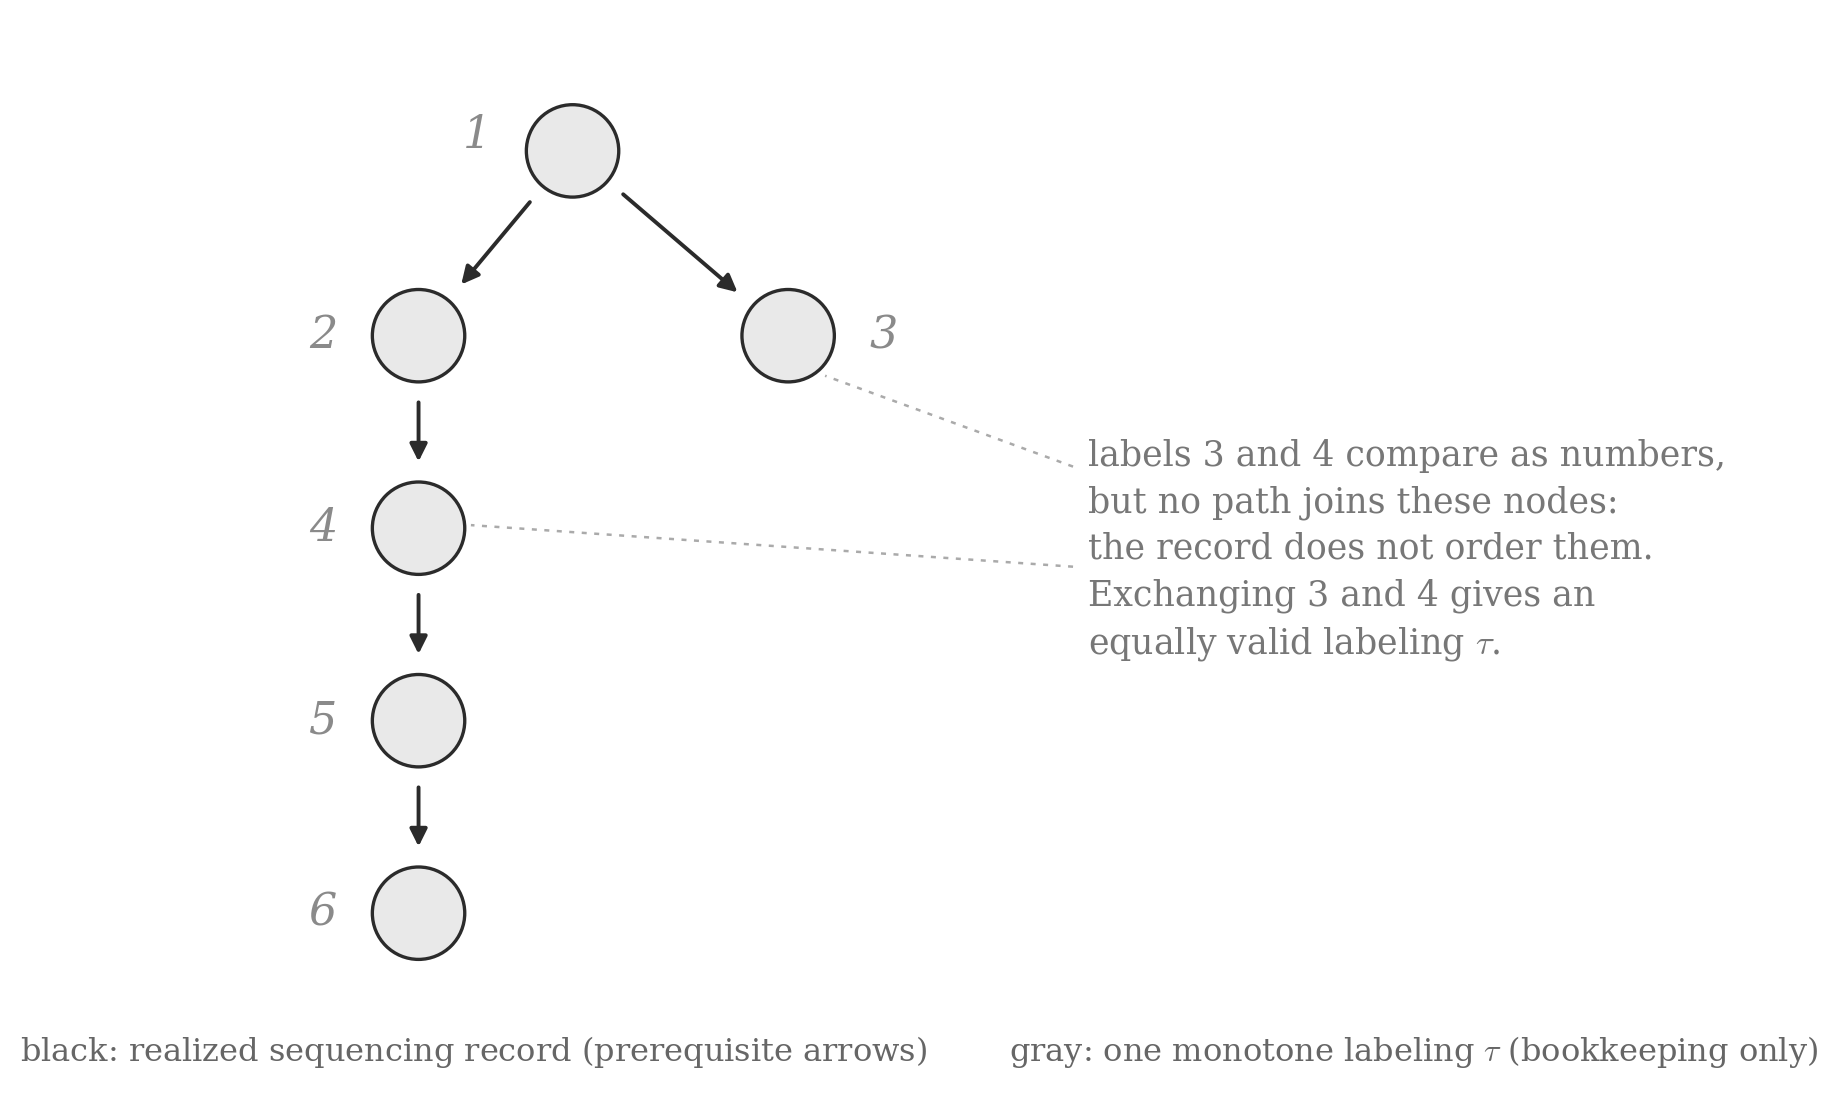
\includegraphics[width=0.85\linewidth]{fig_sequencing_partial_order.png}
\captionsetup{justification=raggedright,singlelinecheck=false}
\caption{\textbf{Sequencing vs.\ temporal reconstruction.} A realized
sequencing record under fixed \(E\), drawn as a strict partial order on
registered restrictions. Black arrows denote immediate prerequisite
relations for addressability restriction only, not temporal succession
or causal flow; comparability is reachability along arrows, and the
absence of a connecting path indicates structural incomparability. Gray
numerals give one possible monotone labeling \(\tau\) of the record,
bookkeeping only, with no metric, rate, or dynamical content. The pair
labeled 3 and 4 is comparable as labels yet incomparable in the record:
no path joins the two nodes, and exchanging their labels yields an
equally valid reconstruction. A temporal reconstruction is thus a
monotone completion of an intrinsically pairwise object: the record
determines a table of pairwise verdicts in which some cells are
genuinely empty, and a linear labeling fills every cell by convention,
compressing the branching, nonlinear path structure of admissibility
restriction into a single coordinate
(Fig.~\ref{fig:sequencing_matrix}).}
\label{fig:sequencing_partial_order}
\end{figure}

\begin{figure}[t]
\centering
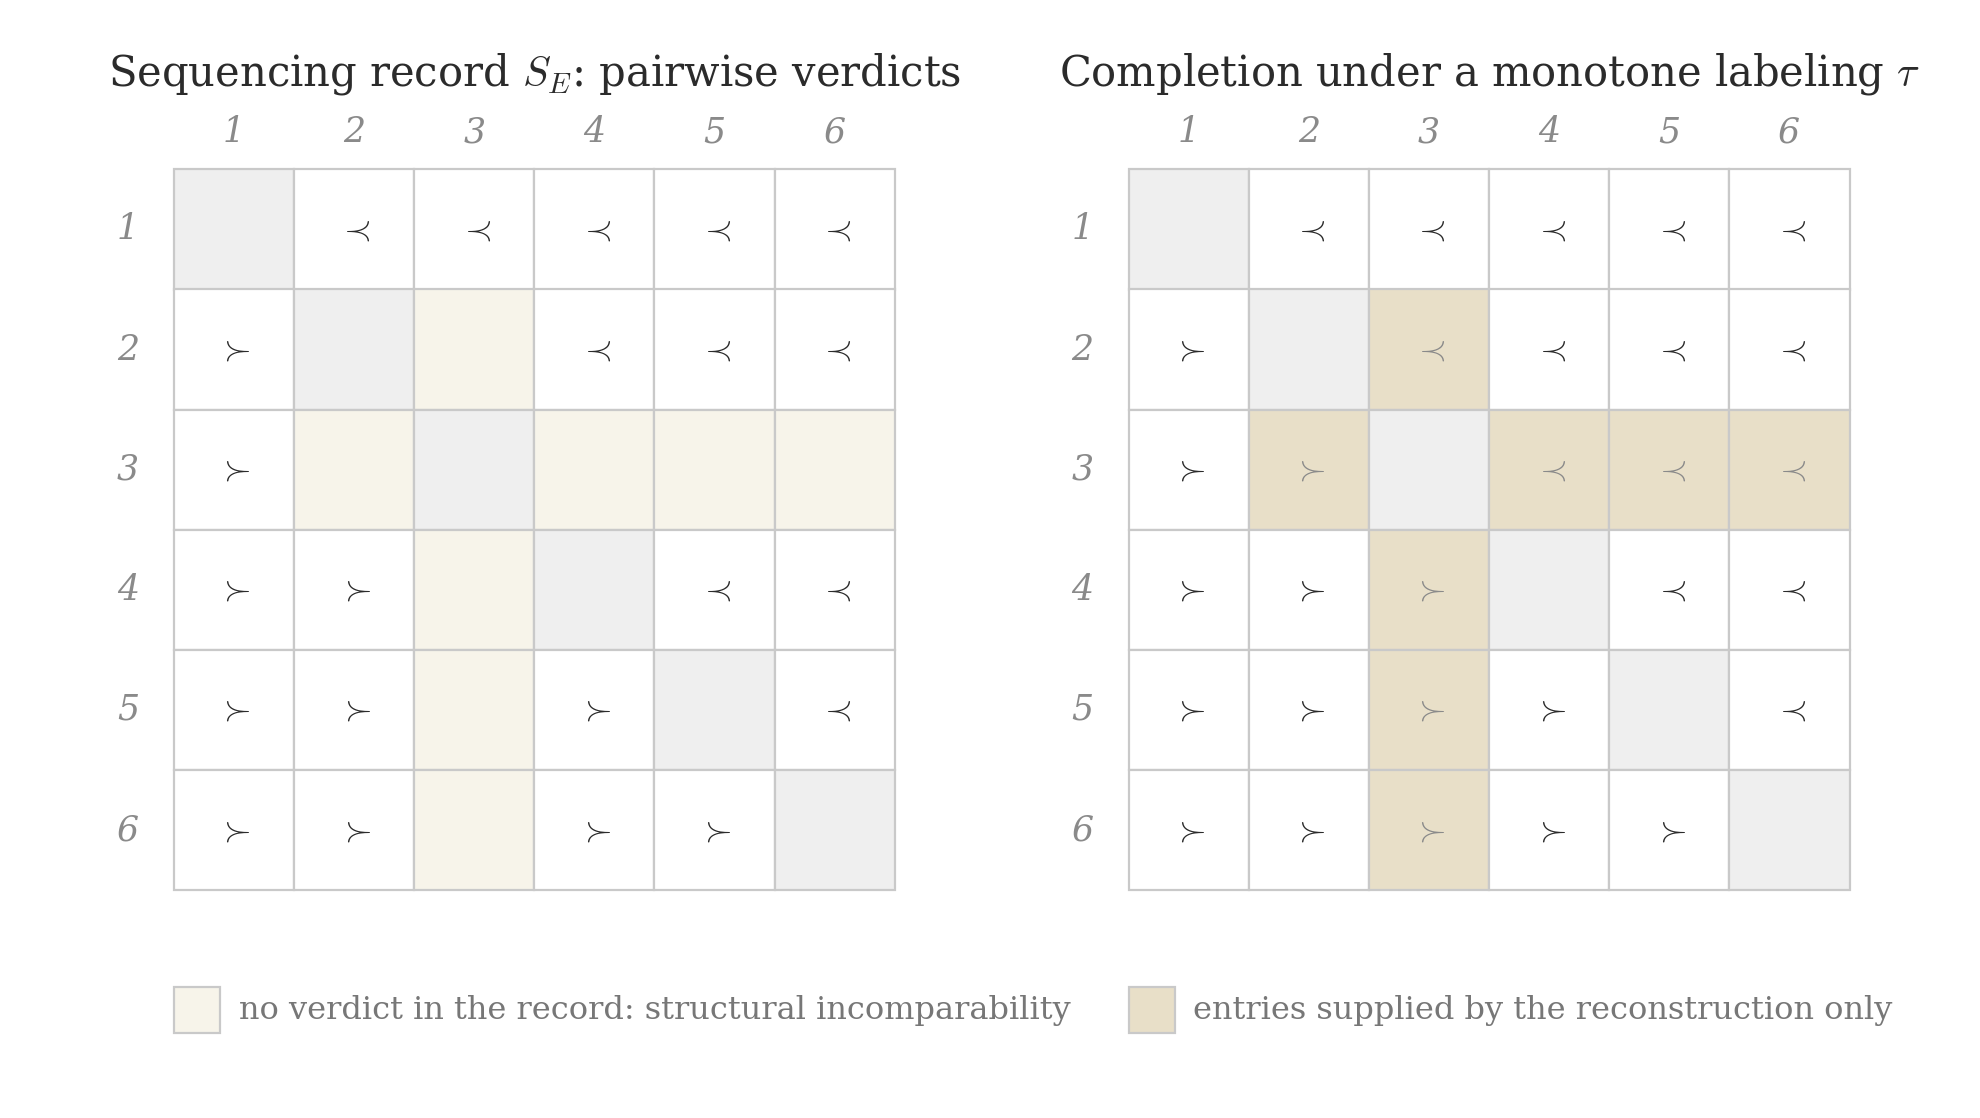
\includegraphics[width=0.95\linewidth]{fig_sequencing_matrix.png}
\captionsetup{justification=raggedright,singlelinecheck=false}
\caption{\textbf{The record as a pairwise table.} The sequencing record
of Fig.~\ref{fig:sequencing_partial_order} written as a comparison
matrix over its six registered restrictions. Entries \(\prec\) and
\(\succ\) are precedence verdicts licensed by reachability in the
record; shaded blank cells are pairs for which the record returns no
verdict. These cells are empty rather than unknown: incomparability is
structural content, not missing data. Right: the completion asserted by
any monotone labeling \(\tau\). A one-dimensional coordinate admits no
empty cells, so every unresolved pair acquires an entry by convention;
the tinted entries are supplied by the reconstruction and carry no
support in the record.}
\label{fig:sequencing_matrix}
\end{figure}

\begin{proposition}[Higher-order witnesses do not eliminate sequencing]
\label{prop:higher_order_witnesses}
Fix a classical context \(E\) and a realized sequencing record \(S_E\),
understood as a strict partial order on registered restrictions under
fixed \(E\). Let \(\mathcal K_E\) be any set and let
\[
W_E:S_E\to\mathcal K_E
\]
be a map defined only from the \(E\)-indexed admissibility,
compatibility, addressability, connectivity, neighbourhood, measure, and
sequencing structure already present under fixed \(E\). Then:
\begin{enumerate}[label=(\roman*)]
\item \(W_E\) may classify, compress, or faithfully represent elements
of \(S_E\);
\item if \(W_E\) is non-injective, sequencing distinctions within
the fibres of \(W_E\) are lost and not recoverable from the image
alone;
\item if \(W_E\) is injective, the image
\(W_E(S_E)\subseteq\mathcal K_E\) is in bijection with \(S_E\), but
does not itself carry the admissibility, compatibility, addressability,
connectivity, neighbourhood, measure, or continuation structure of the
framework unless those structures are explicitly transported or
reconstructed;
\item in no case does \(W_E\) rewrite, eliminate, or supersede \(S_E\)
under fixed \(E\).
\end{enumerate}
\end{proposition}

\begin{proof}
\(S_E\) is a realized acyclic ordering relation equipped with
context-indexed admissibility, compatibility, addressability, and any
declared structural data needed for the construction. The witness
\(W_E\) is defined on \(S_E\) and therefore depends on already-realized
structure.

\emph{Non-injective case.} If \(W_E\) is non-injective, there exist
distinct \(s_1,s_2\in S_E\) with
\[
W_E(s_1)=W_E(s_2).
\]
Any ordering, compatibility, addressability, connectivity, or
structural distinction between \(s_1\) and \(s_2\) is absent from the
image. Since \(S_E\) is not recoverable from \(W_E(S_E)\), the witness
compresses the sequencing record and cannot replace it.

\emph{Injective case.} If \(W_E\) is injective, \(W_E\) establishes a
set-theoretic bijection
\[
S_E\cong W_E(S_E).
\]
However, \(\mathcal K_E\) is an arbitrary codomain. A bijection of
underlying sets does not automatically transport the framework's
context-indexed structure. In particular, the objects
\[
\mathcal A(E),
\qquad
\mathrm{Compat}_E,
\qquad
\sim_E,
\qquad
\Gamma_E,
\qquad
\mathcal N_E,
\qquad
\mu_E,
\]
and the continuation relation are defined on \(\Phi\) or on admissible
domains within \(\Phi\), not on \(\mathcal K_E\) by default. If
\(\mathcal K_E\) is independently equipped with transported versions of
these structures, then \(W_E\) is a relabeling or representation of
\(S_E\), not a replacement for it.

Since realized ordering is not rewritten within a fixed-context
analysis, and since \(W_E\) is defined on that ordering, \(W_E\)
cannot modify its own input. Items (i)--(iv) follow.
\end{proof}

\begin{remark}[Temporal reconstruction as a witness]
\label{rem:temporal_reconstruction_witness}
The monotone labelings of
Fig.~\ref{fig:sequencing_partial_order} are witnesses in the sense of
Proposition~\ref{prop:higher_order_witnesses} with
\(\mathcal K_E=\mathbb N\). An injective such labeling realizes case
(iii) in a strong form: the codomain carries its own total order, under
which every pair of images is comparable, whereas comparability in
\(S_E\) may be strictly coarser. The surplus comparisons introduced by
the codomain are exactly the conventionally filled cells of
Fig.~\ref{fig:sequencing_matrix}; they are structure of \(\mathbb N\),
not structure of \(S_E\), and no choice of monotone labeling removes
them. Temporal reconstruction is therefore witness formation, and its
apparent total order is inherited from the codomain rather than
recorded in \(S_E\).
\end{remark}

\begin{remark}[Structural analogy with activity without leverage]
\label{rem:structural_analogy_witnesses}
The role of higher-order pattern witnesses is structurally analogous to
the activity-without-leverage results developed later in the framework.
In that setting, internal activity, such as variance, correlations, or
periodicity, does not by itself furnish a rectifiable monotone or
extractable work under fixed \(E\). Here, higher-order pattern structure
similarly does not furnish a replacement for the underlying sequencing
record.

In both cases, internal richness is classified but not converted into
external leverage, state-conditioned control, or new ordering relations.
SSAF enforces a general principle: structural richness under fixed \(E\)
does not imply operational reducibility, controllable transformation, or
rewriting of realized ordering.
\end{remark}

\subsubsection{Clock Reconstruction}
\label{subsubsec:clock_reconstruction}

SSAF takes realized ordering as primary. An operational time parameter
appears only after an observer correlates stable ordering markers within
a domain~\cite{Rovelli1991,PageWootters1983,GambiniPullin2007}.

Let \(\tau\) denote an abstract non-metric ordering label. Observers
construct an operational time variable
\begin{equation}
t = \mathcal{R}(\tau;\,E),
\label{eq:clock_reconstruction_map}
\end{equation}
where \(\mathcal{R}\) is a non-unique observer-defined reconstruction
map, defined only where suitable ordering markers remain addressable.
Outside such domains, \(t\) is undefined.

No global regularity of \(\mathcal{R}\) is assumed. Differences in
reconstructed time reflect reconstruction conventions and
domain-of-definition limits, not primitive temporal structure.

\paragraph{Articulation density.}

Let \(N(\tau)\) be the nondecreasing count of addressably recorded
ordering markers up to label \(\tau\). Where \(N\) admits an
absolutely-continuous representative, define
\[
\delta(\tau)
:=
\frac{dN}{d\tau}
\quad
\text{defined a.e.}
\]
Otherwise, use the finite-difference form
\[
\delta_{\Delta\tau}(\tau)
:=
\frac{N(\tau+\Delta\tau)-N(\tau)}{\Delta\tau}.
\]

Larger \(\delta\) corresponds to finer operational articulation of a
reconstruction record. Where \(\tau\) is not reconstructable,
\(\delta\) is undefined.

This diagnostic is distinct from the ordering-density diagnostic
\(\delta_E^{\mathrm{ord}}(W)\), which measures admissible-set
restriction over a finite sequencing window using \(\mu_E\). The present
quantity \(\delta(\tau)\) counts reconstruction markers; it does not
measure admissible-set contraction.

\begin{convention}[Clock reconstruction is post-ordering]
\label{conv:clock_reconstruction_postorder}
Any \(t=\mathcal{R}(\tau;E)\) is an observer-level reconstruction
defined only where ordering markers are addressable. It does not modify
admissibility, compatibility, connectivity, neighbourhood structure,
admissibility measure, restriction, or sequencing, and is not a licensed
input to NS1-consistent rate data or map-family
selection~\cite{BreuerPetruccione2002,Zurek2005}.
\end{convention}

\subsubsection{Amplification of Clock Drift}
\label{subsubsec:clock_drift_amplification}

Convention~\ref{conv:clock_reconstruction_postorder} fixes clock
reconstruction as post-ordering bookkeeping. The following identity shows
that such bookkeeping has nontrivial second-derivative consequences
indexed by \(E\) alone: clock drift couples into reconstructed second
derivatives through a factor \(\alpha(\tau)^{-3}\) that applies to any
sequencing-indexed descriptor. The cosmological instance is developed in
Toy~M (Appendix~\ref{appE:LCDM_dictionary}) and mapped in Appendix E.

\paragraph{Derivative structure.}

Let \(a(\tau)\) be any sequencing-indexed descriptor and suppose the
reconstructed clock satisfies
\[
\frac{dt}{d\tau}
=
\alpha(\tau),
\qquad
\alpha(\tau)>0.
\]
Let
\[
\alpha'(\tau)
:=
\frac{d\alpha}{d\tau}.
\]
Then
\[
\frac{da}{dt}
=
\frac{1}{\alpha(\tau)}
\frac{da}{d\tau},
\]
and
\begin{equation}
\frac{d^2 a}{dt^2}
=
\frac{1}{\alpha(\tau)^2}
\frac{d^2 a}{d\tau^2}
-
\frac{\alpha'(\tau)}{\alpha(\tau)^3}
\frac{da}{d\tau}.
\label{eq:clock_drift_second_derivative}
\end{equation}

\paragraph{Amplification mechanism.}

When the sequencing-indexed descriptor has vanishing second derivative,
\[
\frac{d^2 a}{d\tau^2}=0,
\]
the reconstructed second derivative reduces to
\begin{equation}
\frac{d^2 a}{dt^2}
=
-
\frac{\alpha'(\tau)}{\alpha(\tau)^3}
\frac{da}{d\tau}.
\label{eq:clock_drift_amplified_case}
\end{equation}

The factor \(\alpha(\tau)^{-3}\) governs how drift in \(\alpha\)
propagates into the reconstructed second derivative. In regimes where
\(\alpha(\tau)\) is small along the chain, corresponding to a slow
operational clock, \(\alpha(\tau)^{-3}\) is large and small drift in
\(\alpha\) reconstructs as pronounced second-derivative behavior in
\(t\). In fast-clock regimes, drift is attenuated. The amplification
regime is therefore the slow-clock regime.

\begin{proposition}[Drift Amplification]
\label{prop:drift_amplification}
Let \(\alpha'(\tau)<0\) and \(da/d\tau>0\) on an interval, with
\(\alpha(\tau)\) bounded away from zero. Then, along that interval and
under
\[
\frac{d^2 a}{d\tau^2}=0,
\]
one has
\begin{equation}
\frac{d^2 a}{dt^2}
=
-
\frac{\alpha'(\tau)}{\alpha(\tau)^3}
\frac{da}{d\tau}
>
0.
\end{equation}
The statement is symmetric under joint sign reversal of
\(\alpha'\) and \(da/d\tau\): apparent acceleration of a monotonic
baseline requires \(\alpha'\) and \(da/d\tau\) to have opposite signs.
\end{proposition}

\paragraph{NS1 compliance and scope.}

The amplification channel is available only where \(\alpha(\tau)\), or
equivalently \(\alpha(E_\tau)\) when a context-indexed reconstruction
chain is specified, depends solely on the declared classical-context
record. It may not depend on \(\rho\), outcomes, ensemble
decompositions, or state-derived diagnostics, and it may not be fitted
post hoc as a steering function.

Relaxing any of these conditions converts the reconstruction into a
state- or outcome-conditioned steering channel and removes the
construction from the admissible class. Proposition~\ref{prop:drift_amplification}
therefore identifies both the channel through which reconstruction-level
second-derivative effects enter and the discipline under which those
effects remain structurally attributable to context-indexed
reconstruction rather than to state content.

The cosmological reading of this mechanism appears in Toy~XIII
(Toy~\ref{toy:no_dark_energy}); the \(\Lambda\)CDM dictionary
mapping is in Appendix~\ref{appE:LCDM_dictionary}.

\subsection{Entanglement}
\label{subsec:entanglement}

\emph{Entanglement} denotes non-factorizable joint admissibility under
fixed \(E\) (Eq.~\eqref{eq:nonfactorizable_def_core}):
\(\mathcal{A}_{AB}(E)\) contains at least one jointly admissible
configuration not separable over admissible marginals.

Joint admissibility may be non-factorizable while local marginals
remain well-defined and no signalling is licensed under NS1
(Lemma~\ref{lem:correlation_without_influence})~\cite{Horodecki2009,
Watrous2018}.

\paragraph{Marginal incompatibility.}

There may exist admissible marginals
\[
\rho_A\in\mathcal{A}_A(E),
\qquad
\rho_B\in\mathcal{A}_B(E),
\]
such that no
\[
\rho_{AB}\in\mathcal{A}_{AB}(E)
\]
realizes them simultaneously.

This is a sufficient witness of joint-admissibility restriction beyond
independent marginal admissibility, but it is not asserted equivalent to
entanglement~\cite{Horodecki2009,Watrous2018}.

\paragraph{Envelope non-closure as exclusion witness.}

Joint assignment failures are witnessed by envelope non-closure: empty
intersection of joint envelope constraints excludes a proposed
assignment as a domain-of-definition failure under fixed \(E\), not as
an epistemic limitation or dynamical obstruction.

Correlation language is representational: it is a projection-level
description of joint admissibility constraints under fixed \(E\), with
updating remaining linear CPTP under NS1~\cite{Bell1964,Horodecki2009,
NielsenChuang2010,Watrous2018}.

\subsection{Non-Linkage of Spatial and Temporal Reconstruction}
\label{subsec:nonlinkage_space_time}

Temporal reconstruction parametrizes a realized sequencing record via
\[
t=\mathcal R(\tau;E).
\]
Spatial reconstruction compresses addressable structure from \(\Phi\)
under fixed \(E\). The framework introduces no primitive object that
jointly generates both.

Neither a canonical dependence
\[
t=t(x)
\]
nor
\[
x=x(t)
\]
is fixed. Any coupled \((t,x)\) description is an effective compression
chosen only after a domain and its \(E\)-indexed structure are fixed.
Claims about geometry may not be imported into claims about sequencing
absent an explicit reconstruction choice.

\begin{convention}[Clock reconstruction post-ordering]
\label{conv:clock_reconstruction_postorder_nonlinkage}
Operational time \(t\) is not a primitive parameter but a reconstruction
over a realized ordering label \(\tau\) under fixed classical context
\(E\). Formally,
\begin{equation}
t=\mathcal R(\tau;E),
\end{equation}
with
\begin{equation}
\frac{dt}{d\tau}
=
\alpha(E_\tau),
\qquad
\alpha(E_\tau)>0.
\end{equation}

Here \(\alpha(E_\tau)\) is a context-indexed clock factor depending only
on the classical context along the realized chain, in accordance with
NS1. No dependence on the quantum state \(\rho\), outcomes, ensemble
decompositions, or state-derived diagnostics is permitted.
\end{convention}

This convention is the non-linkage version of
Convention~\ref{conv:clock_reconstruction_postorder}: time coordinates
are reconstructed after ordering, not supplied as primitive structure.

\subsection{Structure}
\label{subsec:structure}

\begin{definition}[Structure]
\label{def:structure_SSAF}
\emph{Structure} denotes persistent relational organization in \(\Phi\)
that is well-posed under fixed \(E\) and its \(E\)-indexed
admissibility, compatibility, addressability, connectivity,
neighbourhood, and measure structure.
\end{definition}

Structure is boundary-defined: a relational pattern is licensed only on
domains where the required configurations and relations remain
well-defined under fixed \(E\). These boundaries are limits of
admissibility, compatibility, interface addressability, or declared
structural organization; they are not spatial surfaces.

\begin{definition}[Pattern-supported structure domain]
\label{def:pattern_supported_domain}
Fix \(E\), admissible set
\[
\mathcal{A}(E)\subseteq\Phi,
\]
and a relational predicate \(\mathsf{P}\) of arity \(m\geq 2\) licensed
only on a stated \(E\)-indexed joint envelope
\[
\mathcal{E}^{\mathsf P}_E\subseteq\Phi^m.
\]

A \emph{pattern-supported domain} is any maximal subset
\[
\mathcal{S}^{\mathsf P}_E(\rho)
\subseteq
\mathcal{A}(E)
\]
such that:
\begin{enumerate}[label=(\roman*), leftmargin=2.2em]
\item \(\rho\in\mathcal{S}^{\mathsf P}_E(\rho)\);
\item \(\mathsf P\) is licensed throughout: every \(m\)-tuple from
\[
\bigl(\mathcal{S}^{\mathsf P}_E(\rho)\bigr)^m
\]
lies in \(\mathcal{E}^{\mathsf P}_E\).
\end{enumerate}

When such a domain exists, \(\rho\) is \emph{structurally persistent for
\(\mathsf P\) under \(E\)}.
\end{definition}

A pattern-supported domain is not automatically a compatibility
envelope, connected component of \(\Gamma_E\), neighbourhood under
\(\mathcal N_E\), basin, or measured region under \(\mu_E\). Those
identifications require explicit model-specific assumptions.

\begin{definition}[Recursion]
\label{def:recursion_structural_closure}
Fix \(E\) and a family
\[
\{\sim^{(k)}_E\}_k
\]
of progressively coarser addressability relations. \emph{Recursion}
denotes closure of \(\mathsf P\) under this coarsening: for each \(k\),
the envelope \(\mathcal{E}^{\mathsf P}_E\) admits a well-defined induced
envelope on
\[
(\Phi/{\sim^{(k)}_E})^m,
\]
so \(\mathsf P\) remains licensed at the quotient level.

This is invariance of admissible relational structure under interface
restriction, not a dynamical rule~\cite{Watrous2018,NielsenChuang2010,
Petz1986,Wilde2017}.
\end{definition}

\subsection{Three Structural Results}
\label{sec:three_hard_results}

These results introduce no new primitives. They establish:
(i) bounded addressability entails non-identifiability under a fixed
interface; (ii) envelope non-closure renders a comparison undefined;
and (iii) non-factorizable joint admissibility permits correlation
without influence under NS1.

\paragraph{Interface closure condition (IC\(_E\)).}

Fix \(E\) and \(\mathcal{O}(E)\). Assume that for any admissible
in-domain CPTP map
\[
\mathcal{T}^E:\Phi\to\Phi
\]
and any
\[
M\in\mathcal{O}(E),
\]
the Heisenberg dual satisfies
\[
\mathcal{T}^{E*}(M)\in\mathcal{O}(E).
\]

This is a closure condition on the interface vocabulary, not a dynamical
assumption~\cite{NielsenChuang2010,Watrous2018}.

\section{Structural Primitives}
\label{sec:structural_primitives}

The framework supplements admissibility and compatibility with two
context-indexed structural primitives,
\[
\Gamma_E,
\qquad
\mu_E,
\]
together with a derived neighbourhood assignment \(\mathcal{N}_E\).

These objects describe global organization, structural weight and a
derived notion of local relatedness within the admissible domain.

They introduce no dynamics, no update rules, no admissibility-selection
rules, and no state-dependent evolution. All dependence remains indexed
only by the fixed classical context \(E\).

\subsection{Connectivity Structure}
\label{subsec:connectivity_structure}

The connectivity structure is the ordered pair
\[
\Gamma_E := (\mathcal{A}(E),\mathcal{R}_E),
\]
where
\[
\mathcal{R}_E
\subseteq
\mathcal{A}(E)\times\mathcal{A}(E)
\]
is a context-indexed connectivity relation. Symmetry of
\(\mathcal{R}_E\) is not assumed at the primitive level; the relation
may be directed, and the derived neighbourhood assignment of
Section~\ref{subsec:neighbourhood_structure} is accordingly stated as
an out-neighbourhood. Where a specific construction imposes symmetry,
that identification is model-level and is marked at the point of use.

The purpose of \(\Gamma_E\) is to record the global organization of
admissible structure under fixed context \(E\).

Connectivity is distinct from admissibility and compatibility:
\begin{itemize}
\item admissibility determines membership in \(\mathcal{A}(E)\);
\item compatibility determines pairwise coexistence;
\item connectivity records large-scale structural organization.
\end{itemize}

\paragraph{Compatibility coherence.}
Connectivity is constrained to respect compatibility. Two admissible
configurations may be connectivity-related only if they are pairwise
compatible:
\[
(\rho,\sigma)\in\mathcal{R}_E
\;\Longrightarrow\;
\mathrm{Compat}_E(\rho,\sigma)=1,
\]
equivalently
\(\mathcal{R}_E \subseteq
\{(\rho,\sigma)\in\mathcal{A}(E)\times\mathcal{A}(E):
\mathrm{Compat}_E(\rho,\sigma)=1\}\).
This fixes how the two relations interact at the framework level.
\(\mathrm{Compat}_E\) delimits which links are available at all, and
\(\Gamma_E\) selects, among compatible pairs, those that carry global
organization. The model-specific identification
\eqref{eq:zdephasing_connectivity}, in which every compatible pair is
connected, is the tight case of this inclusion. That the inclusion can
be strict, so that connectivity is genuinely coarser than compatibility
and neither primitive is derivable from the other, is witnessed via
charge sectors in Toy~\ref{toy:connectivity_strict_separation}.
Under the threshold-shadow grounding worked in
Toy~\ref{toy:threshold_shadow_grounding}, this inclusion is not an
independent assumption: when \(\mathrm{Compat}_E\) and
\(\mathcal R_E\) arise as superlevel sets of a single graded access
functional at thresholds \(\theta_c\le\theta_\gamma\), the
inclusion holds automatically
(Corollary~\ref{cor:toy_shadow_coherence}).

\subsection{Neighbourhood Structure (Derived)}
\label{subsec:neighbourhood_structure}

Local relatedness is not a separate primitive. The neighbourhood
assignment is derived from the connectivity structure \(\Gamma_E\) as
the out-neighbourhood in the connectivity relation:
\[
\mathcal{N}_E(\rho)
:=
\{\sigma\in\mathcal{A}(E):(\rho,\sigma)\in\mathcal{R}_E\}.
\]
\(\mathcal{N}_E(\rho)\subseteq\mathcal{A}(E)\) is therefore notation
for the configurations connectivity-related to \(\rho\), and carries no
information beyond \(\Gamma_E\).

No metric notion of distance is assumed.

\subsection{Admissibility Measure}
\label{subsec:admissibility_measure}

The admissibility measure is the map
\[
\mu_E :
\mathcal{P}(\mathcal{A}(E))
\rightarrow
[0,\infty].
\]

The measure \(\mu_E\) assigns structural weight to admissible regions.
At the primitive level it is a monotone set function and nothing more:
\[
U\subseteq V\subseteq\mathcal A(E)
\quad\Longrightarrow\quad
\mu_E(U)\leq \mu_E(V).
\]

Concentration, density, dispersion, relative size and occupancy are
derived comparisons built from \(\mu_E\), formed as ratios or
differences of admissible-set weights, and are not themselves
primitive. The ordering-density diagnostic
\(\delta^{E}_{\mathrm{ord}}\) is one such derived quantity.

The admissibility measure is distinct from probability measures used in
representational constructions, and it does not determine
admissibility, compatibility, update-family selection, resolution rates
or NS1-licensed dynamics. Its role is purely structural.

\begin{remark}[Terminology]
The word ``measure'' is used here in the loose sense of a monotone set
function. No $\sigma$-algebra is fixed, and $\sigma$-additivity,
finite additivity and normalization are deliberately not assumed at
the primitive level. Where a specific construction equips $\mu_E$ with
additivity or a distinguished domain, that structure is model-level
and is marked as such at the point of use, in accordance with the
derivation exception of
Section~\ref{sec:separation_discipline}.
\end{remark}

\subsection{Primitive Separation}
\label{subsec:primitive_separation}

The primitive structural objects have distinct responsibilities:

\begin{center}
\begin{tabular}{ll}
\hline
Object & Responsibility \\
\hline
\(\mathcal{A}(E)\) & Membership \\
\(\mathrm{Compat}_E\) & Pairwise coexistence \\
\(\Gamma_E\) & Connectivity structure \\
\(\mu_E\) & Structural weight (monotone set function) \\
\(\sim_E\) & Addressability \\
\hline
\end{tabular}
\end{center}

\(\mathcal{N}_E\) is derived from \(\Gamma_E\) and is omitted from the
table of primitives. No primitive should be interpreted as performing
the role of another unless an explicit derivation is provided.

\subsection{Separation Discipline}
\label{sec:separation_discipline}

Each object carries a single structural role, and role transfer between
objects is not permitted unless an explicit derivation is given. The
boundaries are stated once here. Throughout the rest of the paper a
reminder of any boundary below is a reference to this section rather
than a restatement.

\paragraph{Roles.}
\begin{enumerate}[label=(\roman*), leftmargin=2.4em]
\item \(\mathcal{A}(E)\) fixes membership and nothing else.
\item \(\mathrm{Compat}_E\) records pairwise coexistence only. It carries
no topology, geometry, neighbourhood, connectivity, measure, or
concentration.
\item \(\Gamma_E\) records global organization only. It carries no
metric, locality, embedding, sequencing, or dynamical content.
\item \(\mu_E\) records structural weight only, as a monotone set
function. Concentration, density, dispersion and relative size are
derived from it and are not separate objects.
\item \(\mathcal{O}(E)\) and \(\sim_E\) record operational
distinguishability only. Addressability is an interface fact, not an
ontological one, and \(\sim_E\) never refines or restricts
\(\mathcal{A}(E)\).
\item \(\mathcal{N}_E\) is derived from \(\Gamma_E\) and carries no
information beyond it.
\item \(\mathrm{Coh}_E\) is diagnostic only. It never enters
admissibility, compatibility, update-family selection, or NS1-licensed
dynamics.
\item Representational and bookkeeping objects, including the sequencing
label and the reconstruction maps, record or relabel structure and
never generate it.
\end{enumerate}

\paragraph{Global boundaries.}
For every object above the following hold unless an explicit
construction states otherwise:
\begin{enumerate}[label=(\alph*), leftmargin=2.4em]
\item no object implies a topology, a metric, a geometry, a locality
structure, or a spacetime embedding;
\item no object introduces dynamics, updating remains linear and CPTP
and no new microdynamics are added at any point;
\item no object depends on the quantum state \(\rho\), in accordance
with the dependency discipline of NS1.
\end{enumerate}

\paragraph{Derivation exception.}
A boundary may be crossed only by a construction that says so. Where a
particular instantiation identifies connectivity with compatibility, or
builds a neighbourhood from a relation, that identification is
model-specific and is marked as such at the point of use. Absent such a
mark, the roles above are disjoint.


\section{Structural Consequences of Fixed-Context Addressability}
\label{sec:structural_consequences_addressability}

\begin{theorem}[Addressability stable under admissible updating]
\label{thm:fixed_context_no_retro_addressability}
Fix \(E\) with interface \(\mathcal{O}(E)\) and assume
\emph{(IC\(_E\))}. For any admissible in-domain CPTP map
\(\mathcal{T}^E\),
\[
\rho \sim_E \sigma
\;\Longrightarrow\;
\mathcal{T}^E(\rho) \sim_E \mathcal{T}^E(\sigma).
\]
Under fixed \(E\), no admissible in-domain operation refines the
quotient
\[
\Phi/{\sim_E}.
\]
\end{theorem}

\begin{proof}
Let \(M\in\mathcal{O}(E)\). By Schrödinger-Heisenberg duality,
\[
\mathrm{Tr}\bigl(M\,\mathcal{T}^E(\rho)\bigr)
=
\mathrm{Tr}\bigl(\mathcal{T}^{E*}(M)\rho\bigr).
\]
By \((\mathrm{IC}_E)\),
\[
\mathcal{T}^{E*}(M)\in\mathcal{O}(E).
\]
Since \(\rho\sim_E\sigma\),
\[
\mathrm{Tr}\bigl(\mathcal{T}^{E*}(M)\rho\bigr)
=
\mathrm{Tr}\bigl(\mathcal{T}^{E*}(M)\sigma\bigr).
\]
Therefore
\[
\mathrm{Tr}\bigl(M\,\mathcal{T}^E(\rho)\bigr)
=
\mathrm{Tr}\bigl(M\,\mathcal{T}^E(\sigma)\bigr)
\]
for all \(M\in\mathcal{O}(E)\), hence
\[
\mathcal{T}^E(\rho)\sim_E\mathcal{T}^E(\sigma).
\]
\end{proof}

\begin{theorem}[No escape from interface traps under bounded admissibility]
\label{thm:toy_preview_no_escape}
If
\[
\mathcal{U}_E(o,a)=\varnothing
\]
for some realizable pair \((o,a)\), then no policy \(\pi\) can produce
a legal continuation from that pair under fixed interface and fixed
context \(E\), regardless of any bounded preview variable \(p\).
\end{theorem}

\begin{proof}
The condition
\[
\mathcal{U}_E(o,a)=\varnothing
\]
means there is no
\[
u\in\mathcal{U}
\]
such that
\[
F_E(\rho,a,u)\in\mathcal{A}(E)\cap\mathcal{E}_E(\rho)
\]
for all \(\rho\in o\).

A policy \(\pi\) has access only to interface-visible data \((o,a,p)\)
and must output some \(u\in\mathcal{U}\). Since no such legal \(u\)
exists,
\[
\pi(o,a,p)\notin\mathcal{U}_E(o,a)
\]
for any \(p\). Hence no policy yields a legal continuation from
\((o,a)\).
\end{proof}

\begin{remark}[Operational consequence: preview does not defeat domain-of-definition boundaries]
\label{rem:preview_no_escape}
The other structural theorems establish that admissibility boundaries
are domain-of-definition failures rather than dynamical prohibitions.
Theorem~\ref{thm:toy_preview_no_escape} makes this operational: even an
agent with advance knowledge of incoming constraints cannot construct a
legal continuation when the admissible update set is empty.

The obstruction is not informational, since the agent may know exactly
what is coming. The obstruction is structural: no element of the action
space satisfies fiberwise legality. A worked witness is provided in
Sec.~\ref{toy:preview_worked_witness}.
\end{remark}

\begin{theorem}[Envelope non-closure yields domain-of-definition failure]
\label{thm:envelope_nonclosure_domain_failure}
Fix \(E\) and a finite family
\[
\{\mathcal{E}^{(k)}_{AB}(E)\}_{k\in K}.
\]
If
\[
\mathcal{E}^{(K)}_{AB}(E)
:=
\bigcap_{k\in K}\mathcal{E}^{(k)}_{AB}(E)
=
\varnothing,
\]
then:

\begin{enumerate}[label=(\roman*), leftmargin=2.2em]
\item no jointly admissible witness exists satisfying all constraints;
\item any ordering, comparison, or diagnostic requiring such a witness
is \emph{undefined} within the \(E\)-indexed description.
\end{enumerate}
\end{theorem}

\begin{proof}
Item (i) is immediate from emptiness. For (ii), predicates defined only
on inputs with an admissible witness have no value when that domain is
empty. The corresponding claim is undefined, not merely
unknown~\cite{Isham1995,AbramskyBrandenburger2011}.
\end{proof}

\begin{theorem}[Operational consistency implies CPTP]
\label{thm:operational_consistency_implies_cptp}
Fix \(E\). Let
\[
\mathfrak{U}_E:
\mathcal{D}(\mathcal{H})
\to
\mathcal{D}(\mathcal{H})
\]
satisfy:

\begin{enumerate}[label=(\roman*), leftmargin=2.2em]
\item convex-linearity;
\item state validity:
\[
\mathfrak{U}_E(\rho)\succeq 0,
\qquad
\mathrm{Tr}(\mathfrak{U}_E(\rho))=1;
\]
\item ancilla consistency:
\[
\mathfrak{U}_E\otimes\mathrm{id}_{\mathcal K}
\]
maps joint states to joint states for every finite ancilla
\(\mathcal K\).
\end{enumerate}

Then \(\mathfrak{U}_E\) extends uniquely to a linear CPTP map admitting
a Kraus/Stinespring representation.
\end{theorem}

\begin{proof}
Convex-linearity gives affine-linearity on
\(\mathcal{D}(\mathcal{H})\), extending uniquely to a linear map on
trace-class operators. State validity gives positivity and trace
preservation. Ancilla consistency enforces complete positivity. The map
is therefore CPTP and admits Kraus/Stinespring
form~\cite{Choi1975,Stinespring1955,Watrous2018}.
\end{proof}

NS1 is enforced as a dependency discipline on families
\[
\{\mathfrak{U}_E\}.
\]
Parameterization is indexed only by \(E\), never by \(\rho\), outcomes,
ensemble decompositions, or state-derived diagnostics. Under this
discipline, CPTP updating is representation-consistent and introduces
no signalling channels~\cite{Gisin1989,Gisin1990,Polchinski1991}.

\section{Operator Algebra and Admissible Structure}
\label{sec:operator_algebra}

This section fixes admissible operator classes and the permitted
dependency structure of maps and generators under NS1. It introduces no
primitives beyond Core Definitions.

\subsection{Operator Domain and Configuration Space}
\label{subsec:operator_domain}

All operators act on \(\mathcal{H}\); configurations are density
operators
\[
\rho\in\mathcal{D}(\mathcal{H})=\Phi
\]
\cite{Kraus1983,NielsenChuang2010,Watrous2018,Wilde2017}.

SSAF introduces no classical phase space, canonical coordinates,
Hamiltonian flow, metric geometry, topology, connectivity relation,
neighbourhood assignment, or measure as background structure on bare
\(\Phi\).

Descriptors are context-indexed relations, predicates, structural
objects, or functionals on \(\Phi\) or on admissible domains
\(\mathcal A(E)\subseteq\Phi\), induced by stated operator choices,
interfaces, and structural assignments under fixed \(E\).

Geometric language is used only for representational bookkeeping unless
explicitly supplied by a model-specific construction
\cite{BengtssonZyczkowski2006}.

\subsection{Admissible Operator Classes}
\label{subsec:admissible_operator_classes}

SSAF uses the standard operator classes of quantum theory:
self-adjoint operators as observables, unitaries as closed-system
transformations, and CPTP maps as open-system updating
\cite{NielsenChuang2010,Watrous2018}. No additional operator families
are introduced as primitives.

Operator choices do not by themselves determine admissibility,
compatibility, connectivity, neighbourhood structure, admissibility
measure, sequencing, or resolution-rate data. Those objects remain
indexed by the fixed classical context \(E\).

\subsection{Resolution and CPTP Updating}
\label{subsec:resolution_cptp_updating}

\emph{Resolution} is an interface-level restriction of addressable
distinctions under fixed \(E\)
(Sec.~\ref{subsec:resolution_without_collapse}). When updating is
represented, it is represented by linear CPTP maps
\[
\rho\mapsto\mathcal{T}^E(\rho),
\]
expressible in Kraus form. Continuous-parameter semigroup updating under
fixed \(E\) is represented in GKSL/Lindblad form
\cite{Kraus1983,Lindblad1976,Gorini1976}.

\begin{proposition}[CPTP updating is outcome-neutral under fixed \(E\)]
\label{prop:cptp_outcome_neutral}
Admissible updating is represented by linear CPTP maps
\[
\mathcal{T}^E:\Phi\to\Phi
\]
with Kraus and, when applicable, GKSL/Lindblad forms as standard
representations. This layer introduces no state-indexed map-selection
rule, no outcome-indexed modification rule, and no state-dependent
retuning of \(\Gamma_E\), \(\mathcal N_E\), or \(\mu_E\) under fixed
\(E\).
\end{proposition}

\begin{proof}
Kraus and GKSL/Lindblad forms are standard representations of linear
CPTP maps and CPTP semigroups respectively. SSAF introduces no
additional rule conditioning map choice on \(\rho\), decompositions of
\(\rho\), outcome-indexed data, or state-derived diagnostics under fixed
\(E\). State-dependent retuning of the structural primitives is
excluded by
Corollary~\ref{cor:structural_primitives_cannot_be_state_retuned}.
\end{proof}

A concrete single-qubit GKSL family satisfying this discipline
(Corollary~\ref{cor:NS1_GKSL_admissible}) is constructed in
Toy~\ref{toy:single_qubit_NS1_safe_GKSL_semigroup},
witnessing that the NS1-compliant update class is nonempty.

\paragraph{Heisenberg dual.}

For any admissible CPTP map \(\mathcal{T}^E\), its adjoint
\[
\mathcal{T}^{E*}:\mathcal{B}(\mathcal{H})\to\mathcal{B}(\mathcal{H})
\]
satisfies
\[
\mathrm{Tr}\bigl(M\,\mathcal{T}^E(\rho)\bigr)
=
\mathrm{Tr}\bigl(\mathcal{T}^{E*}(M)\rho\bigr)
\]
for all
\[
\rho\in\Phi,
\qquad
M\in\mathcal{B}(\mathcal{H}).
\]
This is a representational rewrite and introduces no new primitives.

\subsection{Resolution without Collapse}
\label{subsec:resolution_without_collapse}

Resolution denotes a context-indexed restriction of addressable
distinctions within a realized ordering under fixed \(E\). It is an
interface-level access statement, not a dynamical postulate acting on
\(\Phi\).

Configurations excluded from addressability remain elements of \(\Phi\)
but are non-addressable relative to the realized ordering record and
interface under fixed \(E\).

\begin{proposition}[Resolution does not alter \(\Phi\)]
\label{prop:resolution_not_destruction}
Resolution restricts which distinctions are addressable within a
realized ordering but does not remove, alter, or reparameterize elements
of \(\Phi\). Excluded configurations remain elements of \(\Phi\) and
may be admissible, addressable, or structurally organized differently
under distinct contexts or realized orderings.
\end{proposition}

\begin{proof}
Resolution acts on addressability, record-level distinctions, or
\(\sim_E\)-classes within a stated interface. It does not act on
\(\rho\in\Phi\) as an element of the underlying configuration space. The
set \(\Phi\) is therefore unchanged.
\end{proof}

\subsection{NS1 as an Operator-Level Dependency Constraint}
\label{subsec:NS1_operator_constraint}

For each fixed \(E\), any admissible update family
\[
\{\mathcal{T}^E_\Delta\}_\Delta
\]
consists of linear CPTP maps on \(\Phi\). All map and generator
parameterization data depend only on \(E\) and are independent of
\(\rho\), any ensemble decomposition of \(\rho\), any outcome-indexed
interface data, and any state-derived diagnostic.

The same dependency discipline applies to the structural primitives
\[
\Gamma_E,
\qquad
\mathcal N_E,
\qquad
\mu_E.
\]
They may be used as context-indexed structural data, but they may not be
selected, retuned, or reweighted as functions of the input state,
outcomes, ensemble decompositions, or diagnostics.

This is not a modeling convention but a structural non-signalling
constraint: nontrivial state-conditioned generator selection under fixed
\(E\) produces ensemble-dependent updating that enables signalling by
remote preparation
(Theorem~\ref{thm:fixed_context_generator_selection}).

\begin{corollary}[GKSL admissibility under NS1]
\label{cor:NS1_GKSL_admissible}
When updating is represented by a CPTP semigroup with a GKSL/Lindblad
generator, NS1 requires the Hamiltonian term, Lindblad operators, and
all rate coefficients to depend only on \(E\):
\[
\lambda_\alpha=\lambda_\alpha(E),
\qquad
\frac{\delta\lambda_\alpha}{\delta\rho}=0
\]
\cite{Lindblad1976,Gorini1976,Watrous2018}. This is a direct
specialization of
Theorem~\ref{thm:fixed_context_generator_selection} to the GKSL case.
\end{corollary}

\subsection{Born Weights as Interface Measures}
\label{subsec:born_weights_interface}

Fix \(E\) and a POVM
\[
\{M_k(E)\}_k
\]
on \(\mathcal{H}\). For \(\rho\in\Phi\),
\[
p_k(E\mid\rho)
=
\mathrm{Tr}(M_k(E)\rho),
\qquad
\sum_k p_k=1.
\]

These weights are interface-level measures on the \(E\)-indexed
addressability classes induced by \(\mathcal{O}(E)\). They do not enter
NS1-licensed map or generator parameterization
\cite{Born1926,Gleason1957,Deutsch1999,NielsenChuang2010,Watrous2018}.

Born weights are distinct from the structural admissibility measure
\(\mu_E\). Born weights assign interface-statistical weights to
outcomes or addressability classes for a given configuration \(\rho\).
By contrast, \(\mu_E\) assigns structural weight to admissible regions
inside \(\mathcal A(E)\). Neither object may be used to select
state-conditioned update maps, generators, or resolution-rate data under
fixed \(E\).

This operator-algebra layer adds no measurement postulate and no
modification of standard operator-algebraic updating. Its role is
structural: fixing admissible operator classes and enforcing NS1 as a
restriction on admissible dependencies.

\clearpage

\section{Axioms of State Space Admissibility Framework}
\label{sec:axioms}

These axioms fix SSAF's architecture: a configuration-space ontology in
\(\Phi\), a context-indexed admissibility and compatibility layer, a
context-indexed structural layer, and an NS1 dependency discipline for
admissible updating. Standard quantum objects are used as
representational tools within these constraints~\cite{Watrous2018,NielsenChuang2010}.

\subsubsection*{Axiom 0: Emergent Sequencing
\;(\textit{Ontological, Structural})}
\label{ax:sequencing}

Time is non-primitive. Observable temporal structure is an
observer-level reconstruction of a non-retro-addressable sequencing
relation under fixed \(E\). Sequencing is an acyclic realized ordering
relation over admissible structure; any coordinate \(t\) is
post-ordering bookkeeping only~\cite{PageWootters1983,Rovelli1991,GambiniPullin2007}.

\subsubsection*{Axiom I: Unified Configuration Ontology
\;(\textit{Ontological})}
\label{ax:unified_config_ontology}

All physical systems are represented within a single configuration
space \(\Phi\), with
\[
\Phi=\mathcal{D}(\mathcal{H})
\]
and configurations represented as density operators
\[
\rho\in\mathcal{D}(\mathcal{H}).
\]
The term ``hyperfield'' is used only as prose for this
state-space-first ontology~\cite{Watrous2018}. No external arena,
background spacetime, metric geometry, classical phase space, or
dynamical flow is assumed as primitive.

\subsubsection*{Axiom II: Phase as a Structural Descriptor
\;(\textit{Ontological, Structural})}
\label{ax:phase_fundamental_descriptor}

Phase-relevant descriptors supply primary distinctions used for
compatibility assessment, interface statistics, and reconstruction under
fixed \(E\). ``Phase'' enters only through \(E\)-indexed admissibility,
compatibility, structural organization, declared interface statistics
\[
\mathrm{Tr}(M\rho),
\qquad
M\in\mathcal{O}(E),
\]
or an explicitly stated reconstruction dictionary.

No additional phase space, canonical coordinates, hidden phase
substance, or Hamiltonian flow is introduced as primitive. Spatial and
geometric descriptions, when used, are derived or reconstructed
descriptions of admissible structure in \(\Phi\), not background
assumptions.

\subsubsection*{Axiom III: Coherence Diagnostics
\;(\textit{Structural})}
\label{ax:coherence_diagnostics}

\(\mathrm{Coh}_E(\rho)\) is a diagnostic classifier of persistence of
phase-structured relations relative to a fixed context-indexed
reference. It does not parameterize admissibility, compatibility,
connectivity, neighbourhood structure, admissibility measure,
sequencing, or NS1-licensed update-family data
\cite{Baumgratz2014,Schlosshauer2007}.

\subsubsection*{Axiom IV: State-Space-First Geometry
\;(\textit{Geometric, Structural})}
\label{ax:state_space_first_geometry}

Geometric language is a representational descriptor over admissible
structure in \(\Phi\). It may encode relational distinguishability,
compatibility bookkeeping, connectivity organization, neighbourhood
relations, admissibility concentration, or persistence structure.

For pure configurations this may use projective Hilbert-space geometry;
for general configurations, density-operator state-space geometry
\cite{BengtssonZyczkowski2006,Watrous2018}. No metric, locality,
embedding, topology, manifold structure, or dynamical flow is assumed as
primitive on bare \(\Phi\).

\subsubsection*{Axiom V: Non-Linkage of Space and Time
\;(\textit{Ontological, Constraint})}
\label{ax:nonlinkage_space_time}

Space and time are independent reconstructions. Time parametrizes a
realized sequencing record; space compresses stable addressability,
compatibility, connectivity, or neighbourhood structure in \(\Phi\)
under fixed \(E\). SSAF specifies no canonical linkage between them.

Any coupled spatiotemporal description is an effective compression
chosen only after a domain and its \(E\)-indexed admissibility and
structural objects have been fixed.

\subsubsection*{Axiom VI: Linear CPTP Updating
\;(\textit{Dynamical})}
\label{ax:linear_cptp_updating}

Admissible updating is represented by linear CPTP maps acting on
\(\rho\), consistent with standard open-system quantum structure
\cite{Kraus1983,NielsenChuang2010,Watrous2018}. Continuous-parameter
semigroup representations may use GKSL generators
\cite{Lindblad1976,Gorini1976,BreuerPetruccione2002}. Any family
indexing carries no primitive temporal meaning.

This is not an independent posit.
Theorem~\ref{thm:operational_consistency_implies_cptp} derives linear
CPTP form from convex-linearity, state validity, and ancilla
consistency. It is stated as an axiom only because the updating
discipline it fixes is invoked throughout.

Linear CPTP updating does not select or retune \(\mathcal A(E)\),
\(\mathrm{Compat}_E\), \(\Gamma_E\), \(\mathcal N_E\), or \(\mu_E\) as
a function of \(\rho\), outcomes, ensemble decompositions, or
state-derived diagnostics. Such state-conditioned retuning is excluded
by NS1.

\subsubsection*{Axiom VII: Context-Indexed, State-Independent
Restriction (NS1) \;(\textit{Dynamical, Constraint})}
\label{ax:NS1}

All admissibility restriction, structural assignment, and CPTP
update-family parameterization are indexed only by fixed classical
context \(E\) and are strictly state-independent:
\[
\lambda_\alpha = F_\alpha(E),
\qquad
\frac{\delta\lambda_\alpha}{\delta\rho}=0.
\]

No admissible rate, generator, map-family parameter, connectivity
relation, neighbourhood assignment, admissibility measure, or
reconstruction rule may be selected or retuned as a function of
\(\rho\), ensemble decompositions, outcomes, or state-derived
diagnostics.

This avoids ensemble-dependent updating and preserves non-signalling
consistency~\cite{Gisin1989,Gisin1990,Polchinski1991}. This is likewise
not independent. Theorem~\ref{thm:fixed_context_generator_selection}
derives state-independent fixed-context rate data from affine updating
and non-signalling; it is stated as an axiom for the same architectural
reason.

\subsubsection*{Axiom VIII: Basin Organization as Representational
Compression \;(\textit{Structural, Geometric})}
\label{ax:basin_representational_compression}

Stable organization in \(\Phi\) may be represented by basin-like
structure within admissible domains. Basin language is a
representational compression of admissibility, compatibility,
connectivity, neighbourhood, measure, and persistence structure under
fixed \(E\).

Toroidal or topological basin descriptions may be used only when a
model-specific construction explicitly supplies the corresponding
structure. Basin language is not a primitive geometry, force law,
potential, or dynamical confinement mechanism~\cite{BengtssonZyczkowski2006}.

\subsubsection*{Axiom IX: Unified Stratification
\;(\textit{Structural, Constraint})}
\label{ax:unified_stratification}

All structural distinctions are expressed within a single stratification
of \(\Phi\) under context-indexed admissibility restriction,
compatibility, addressability, connectivity, neighbourhood structure,
admissibility measure, and diagnostic coherence classification.

No independent sector-specific hierarchies, scale-dependent ontologies,
or additional substrate layers are introduced as primitives.

\paragraph*{Axiom classification.}

These axioms fix primitives, permitted dependencies, and
representational organization. Any downstream addition requiring new
primitives or forbidden dependencies constitutes a theory change.

\medskip
\noindent\textbf{Domain boundaries.}

The following records classes of operations and extensions for which
SSAF supplies no definition. Linear CPTP representability and
state-independent parameterization under fixed \(E\) are standing
constraints; sequencing fixes within-ordering non-retro-addressability.
Proposals requiring additional primitives, state- or outcome-indexed
dependencies, or extra substrate ontology are out of
scope~\cite{Watrous2018,NielsenChuang2010,BreuerPetruccione2002}.

\subsection{Update-Family Parameterization Outside NS1/CPTP Scope}
\label{subsec:failure_forbidden_dependencies}

SSAF assigns no theory-internal meaning to update families,
admissibility predicates, structural primitives, reconstruction rules,
or map/generator parameters that depend on \(\rho\), ensemble
decompositions, state-derived diagnostics, or outcome-indexed
data~\cite{Gisin1989,Gisin1990,Polchinski1991,Watrous2018}.

State-conditioned generators, nonlinear update rules, outcome-weighted
parameterizations, state-retuned connectivity relations,
state-retuned neighbourhood assignments, and state-reweighted
admissibility measures are excluded.

Admissibility predicates indexed by future outcomes, global objectives,
or teleological criteria violate the context-indexed structure fixed by
NS1. Postselection and run filtering are record-level procedures
represented as re-indexing of \(E\); they do not alter the
NS1-consistent CPTP representational class~\cite{NielsenChuang2010,
Watrous2018}.

\subsection{Non-Retro-Addressability Boundary}
\label{subsec:failure_retro_addressability}

Within a realized ordering under fixed \(E\), no admissible in-domain
operation re-addresses distinctions excluded by that realized ordering
record. Once a distinction is excluded by sequencing under fixed \(E\),
it is not reintroduced by any admissible in-domain operation under that
same context.

\subsection{Substrate and Additional Ontology Beyond \(\Phi\)}
\label{subsec:failure_substrate_reintroduction}

SSAF introduces no hidden variables, preferred foliations, background
substrates, or auxiliary ontological layers beneath \(\Phi\) as
primitives~\cite{Bell1964}. SSAF does not assume a spacetime manifold,
metric field, foliation, causal graph, topology, connectivity relation,
neighbourhood assignment, or embedding geometry as primitive on bare
\(\Phi\).

Geometric language is a derived or declared representational compression
of admissibility, compatibility, addressability, connectivity,
neighbourhood, measure, and sequencing structure in \(\Phi\) under fixed
\(E\) only.

\subsection{Resource and Drive Principles}
\label{subsec:failure_resource_drive}

SSAF introduces no in-framework map converting ordering density,
articulation density, basin descriptors, connectivity descriptors,
neighbourhood assignments, measure assignments, or regime labels into an
extractable operational resource.

These are classification or diagnostic devices for context-indexed
admissibility and reconstruction under fixed \(E\), not resource
statements. SSAF does not postulate a variational or optimization
principle as a generator; diagnostics and toy metrics classify
configurations under specified constraints and are not dynamical
drivers~\cite{Goldstein2002,Jaynes1957}.

\section{Axiom Roles and Dependency Structure}
\label{sec:axiomatic_minimality}

The axioms fix admissibility, compatibility, sequencing, structural
organization, and the permitted dependency structure for
representational updating under linear CPTP form consistent with NS1.
Each axiom fixes a distinct scope or dependency boundary; changing an
axiom changes the admissible class of descriptions and constitutes a
theory modification.

\paragraph*{Citation policy and dependency record.}
The axioms are architecture-level commitments. Their content is
enforced structurally throughout the framework, by the definitions,
update discipline, and proofs that realize it, rather than invoked
pointwise at each use. This section is accordingly the canonical
dependency record. Table~\ref{tab:axiom_dependency} maps each axiom to
the formal results that enforce or derive its content and to the
Appendix~D unit tests that witness it in finite models; the same unit
tests are grouped thematically in Sec.~\ref{toy:summary}.

\begin{table}[t]
\centering
\footnotesize
\caption{Axiom dependency record. For each axiom: the formal results
that enforce or derive its content, and the finite unit-test
constructions that witness it. Axioms VI and VII are derived
(Sec.~\ref{subsec:axiom_independence}); their rows list the deriving
theorems.}
\label{tab:axiom_dependency}
\begin{tabular}{p{0.24\linewidth}p{0.40\linewidth}p{0.28\linewidth}}
\toprule
\textbf{Axiom} & \textbf{Enforced/derived by} & \textbf{Unit test(s)} \\
\midrule
\hyperref[ax:sequencing]{0: Emergent Sequencing} &
Thm.~\ref{thm:sequencing_strict_partial_order};
Thm.~\ref{thm:fixed_context_no_retro_addressability};
Props.~\ref{prop:causal_ordering_from_contraction},
\ref{prop:partial_causal_order} &
Toys~\ref{toy:nontotal_ordering},
\ref{toy:structural_nontotal_ordering},
\ref{toy:finite_dim_sequencing_no_retro} \\
\addlinespace
\hyperref[ax:unified_config_ontology]{I: Unified Configuration
Ontology} &
Prop.~\ref{prop:resolution_not_destruction} &
Toy~\ref{toy:compatibility_sleeves} \\
\addlinespace
\hyperref[ax:phase_fundamental_descriptor]{II: Phase as a Structural
Descriptor} &
Props.~\ref{prop:wf_density_equiv},
\ref{prop:phase_order_context_indexed},
\ref{prop:envelope_rep_equiv} &
Toy~\ref{toy:envelope_ordering} \\
\addlinespace
\hyperref[ax:coherence_diagnostics]{III: Coherence Diagnostics} &
Prop.~\ref{prop:admissibility_reproduces_dephasing};
Lems.~\ref{lem:coh_no_rate_role},
\ref{lem:coh_no_structural_retuning} &
Toy~\ref{toy:coherence_basin_depth_functional_contraction} \\
\addlinespace
\hyperref[ax:state_space_first_geometry]{IV: State-Space-First
Geometry} &
Props.~\ref{prop:connectivity_strict},
\ref{prop:addressability_strict} &
Toys~\ref{toy:connectivity_strict_separation},
\ref{toy:threshold_shadow_grounding} \\
\addlinespace
\hyperref[ax:nonlinkage_space_time]{V: Non-Linkage of Space and Time} &
Prop.~\ref{prop:drift_amplification} &
Toy~\ref{toy:no_dark_energy} \\
\addlinespace
\hyperref[ax:linear_cptp_updating]{VI: Linear CPTP Updating
(derived)} &
Thm.~\ref{thm:operational_consistency_implies_cptp};
Thm.~\ref{thm:fixed_context_affine_consistency};
Prop.~\ref{prop:cptp_outcome_neutral} &
Toy~\ref{toy:single_qubit_NS1_safe_GKSL_semigroup} \\
\addlinespace
\hyperref[ax:NS1]{VII: NS1 (derived)} &
Thm.~\ref{thm:fixed_context_generator_selection};
Cor.~\ref{cor:fixed_context_rate_independence};
Prop.~\ref{prop:no_steerable_marginals} &
Toys~\ref{toy:single_qubit_NS1_safe_GKSL_semigroup},
\ref{toy:unified_admissibility_erosion},
\ref{toy:correlation_without_influence} \\
\addlinespace
\hyperref[ax:basin_representational_compression]{VIII: Basin
Organization} &
Defs.~\ref{def:coherence_basin_struct},
\ref{def:coherence_margin_struct} &
Toys~\ref{subsec:spin_closure_discreteness},
\ref{toy:coherence_basin_depth_functional_contraction} \\
\addlinespace
\hyperref[ax:unified_stratification]{IX: Unified Stratification} &
Prop.~\ref{prop:addressability_strict};
Prop.~\ref{prop:no_rec_from_quotient} &
Toys~\ref{toy:structure_without_addressability},
\ref{toy:ignition_filamentary} \\
\bottomrule
\end{tabular}
\end{table}

\subsection{Independence and Dependency Status}
\label{subsec:axiom_independence}

For the structural axioms, namely Axiom~0 and Axioms I through V, VIII
and IX, independence holds in the countermodel sense: each may be
omitted or altered while the others are retained, yielding a description
that preserves standard channel representability but introduces
primitives, dependencies, or representational commitments absent from
SSAF.

Axioms VI and VII are of a different status. They are derived rather
than independent:
Theorem~\ref{thm:operational_consistency_implies_cptp} forces CPTP form
and Theorem~\ref{thm:fixed_context_generator_selection} forces the NS1
dependency discipline, from operational consistency and non-signalling
respectively.

They are listed as axioms because the discipline they fix is invoked
throughout the framework, not because they are logically independent of
it. The axiom set is therefore deliberately non-minimal: it states two
consequences explicitly for architectural visibility rather than leaving
them implicit.

\subsection{Role of Each Axiom}
\label{subsec:axiom_necessity}

\begin{itemize}[leftmargin=*]

\item Relaxing \textbf{Sequencing} admits retro-addressable, cyclic, or
rewritable ordering descriptions.

\item Relaxing \textbf{Unified Configuration Ontology} admits additional
substrates beneath \(\Phi\), or an external arena not represented within
the configuration-space ontology.

\item Relaxing \textbf{Phase as a Structural Descriptor} admits
primitive canonical coordinates, hidden phase substances, or Hamiltonian
flow beneath the admissibility and compatibility description.

\item Relaxing \textbf{Coherence Diagnostics} admits coherence as a
dynamical parameter feeding admissibility, compatibility, structural
assignment, or update-family data, in tension with NS1.

\item Relaxing \textbf{State-Space-First Geometry} admits a primitive
metric, locality, topology, manifold structure, connectivity relation,
neighbourhood assignment, or measure prior to admissibility in \(\Phi\).

\item Relaxing \textbf{Non-Linkage} admits a canonical primitive linkage
between spatial and temporal reconstructions.

\item Relaxing \textbf{Linear CPTP Updating} admits
non-completely-positive, nonlinear, or ensemble-dependent updates,
excluded by Theorem~\ref{thm:operational_consistency_implies_cptp}.

\item Relaxing \textbf{NS1} admits state- or outcome-indexed
update-family parameterizations, state-retuned structural primitives,
or state-dependent reconstruction rules.

\item Relaxing \textbf{Basin Organization} admits basin or toroidal
topology as primitive dynamics rather than representational compression
of admissible structure.

\item Relaxing \textbf{Unified Stratification} admits sector-specific
hierarchies, scale-dependent ontologies, or independent structural
layers outside the single \(\Phi\)-based framework.

\end{itemize}

\subsection{No Additional Axioms Required}
\label{subsec:no_additional_axioms}

No additional axioms are required for the core architecture. Proposed
additions are either redundant with existing structural roles or
downstream regime-limited modeling assumptions rather than core
commitments.

In particular, connectivity, neighbourhood structure, and admissibility
measure do not require new axioms beyond the structural primitive layer:
\[
\Gamma_E,
\qquad
\mathcal N_E,
\qquad
\mu_E.
\]
They are context-indexed structural objects, not dynamical laws or
additional ontology.

\paragraph*{Constraint C1 (No Theory-Internal Retuning).}
\label{par:constraint_c1}

SSAF introduces no theory-internal control variables or state-dependent
retuning maps that reweight admissibility, modify update-family
parameters, retune \(\Gamma_E\), reassign \(\mathcal N_E\), reweight
\(\mu_E\), or implement outcome targeting.

Laboratory controls are part of the fixed classical context \(E\).
Operational talk of ``tuning'' is shorthand for re-indexing the
description by a different specified context \(E\).

\section{Fixed-Context Linearity and Non-Retro-Addressability}
\label{sec:NS1_immediate_consequence}

Under fixed \(E\), admissible updating is represented by an
\(E\)-indexed family of linear CPTP maps. Within a realized ordering
record under the same fixed \(E\), distinctions non-addressable relative
to \(\mathcal{O}(E)\) remain non-addressable under any admissible
in-domain updating.

\begin{lemma}[Fixed-context CPTP updating preserves non-addressability]
\label{lem:NS1_CPTP_no_retro}
Fix \(E\) and \(\mathcal{O}(E)\) with induced \(\sim_E\)
(Eq.~\eqref{eq:addressability_relation}). Assume \emph{(IC\(_E\))}:
\[
M\in\mathcal{O}(E)
\quad\Longrightarrow\quad
\mathcal{T}^{E*}_\Delta(M)\in\mathcal{O}(E)
\]
for every admissible in-domain CPTP map \(\mathcal{T}^E_\Delta\).
Assume the label \(\Delta\) is not selected as a function of the input
state, ensemble decomposition, outcome-indexed data, or state-derived
diagnostic, in accordance with NS1. Then
\[
\rho\sim_E\sigma
\;\Longrightarrow\;
\mathcal{T}^E_\Delta(\rho)\sim_E\mathcal{T}^E_\Delta(\sigma).
\]
Admissible in-domain updating under fixed \(E\) does not refine
\[
\Phi/{\sim_E}.
\]
\end{lemma}

\begin{proof}
Let \(M\in\mathcal{O}(E)\). By Schrödinger-Heisenberg duality,
\[
\mathrm{Tr}\bigl(M\,\mathcal{T}^E_\Delta(\rho)\bigr)
=
\mathrm{Tr}\bigl(\mathcal{T}^{E*}_\Delta(M)\rho\bigr).
\]
By \((\mathrm{IC}_E)\),
\[
\mathcal{T}^{E*}_\Delta(M)\in\mathcal{O}(E).
\]
Since \(\rho\sim_E\sigma\),
\[
\mathrm{Tr}\bigl(\mathcal{T}^{E*}_\Delta(M)\rho\bigr)
=
\mathrm{Tr}\bigl(\mathcal{T}^{E*}_\Delta(M)\sigma\bigr).
\]
Hence
\[
\mathrm{Tr}\bigl(M\,\mathcal{T}^E_\Delta(\rho)\bigr)
=
\mathrm{Tr}\bigl(M\,\mathcal{T}^E_\Delta(\sigma)\bigr)
\]
for all \(M\in\mathcal{O}(E)\). Therefore
\[
\mathcal{T}^E_\Delta(\rho)
\sim_E
\mathcal{T}^E_\Delta(\sigma).
\]
NS1 excludes state- or outcome-conditioned map selection
\cite{Gisin1989,Gisin1990,Polchinski1991,Watrous2018,NielsenChuang2010}.
\end{proof}

\begin{figure}[t]
\centering
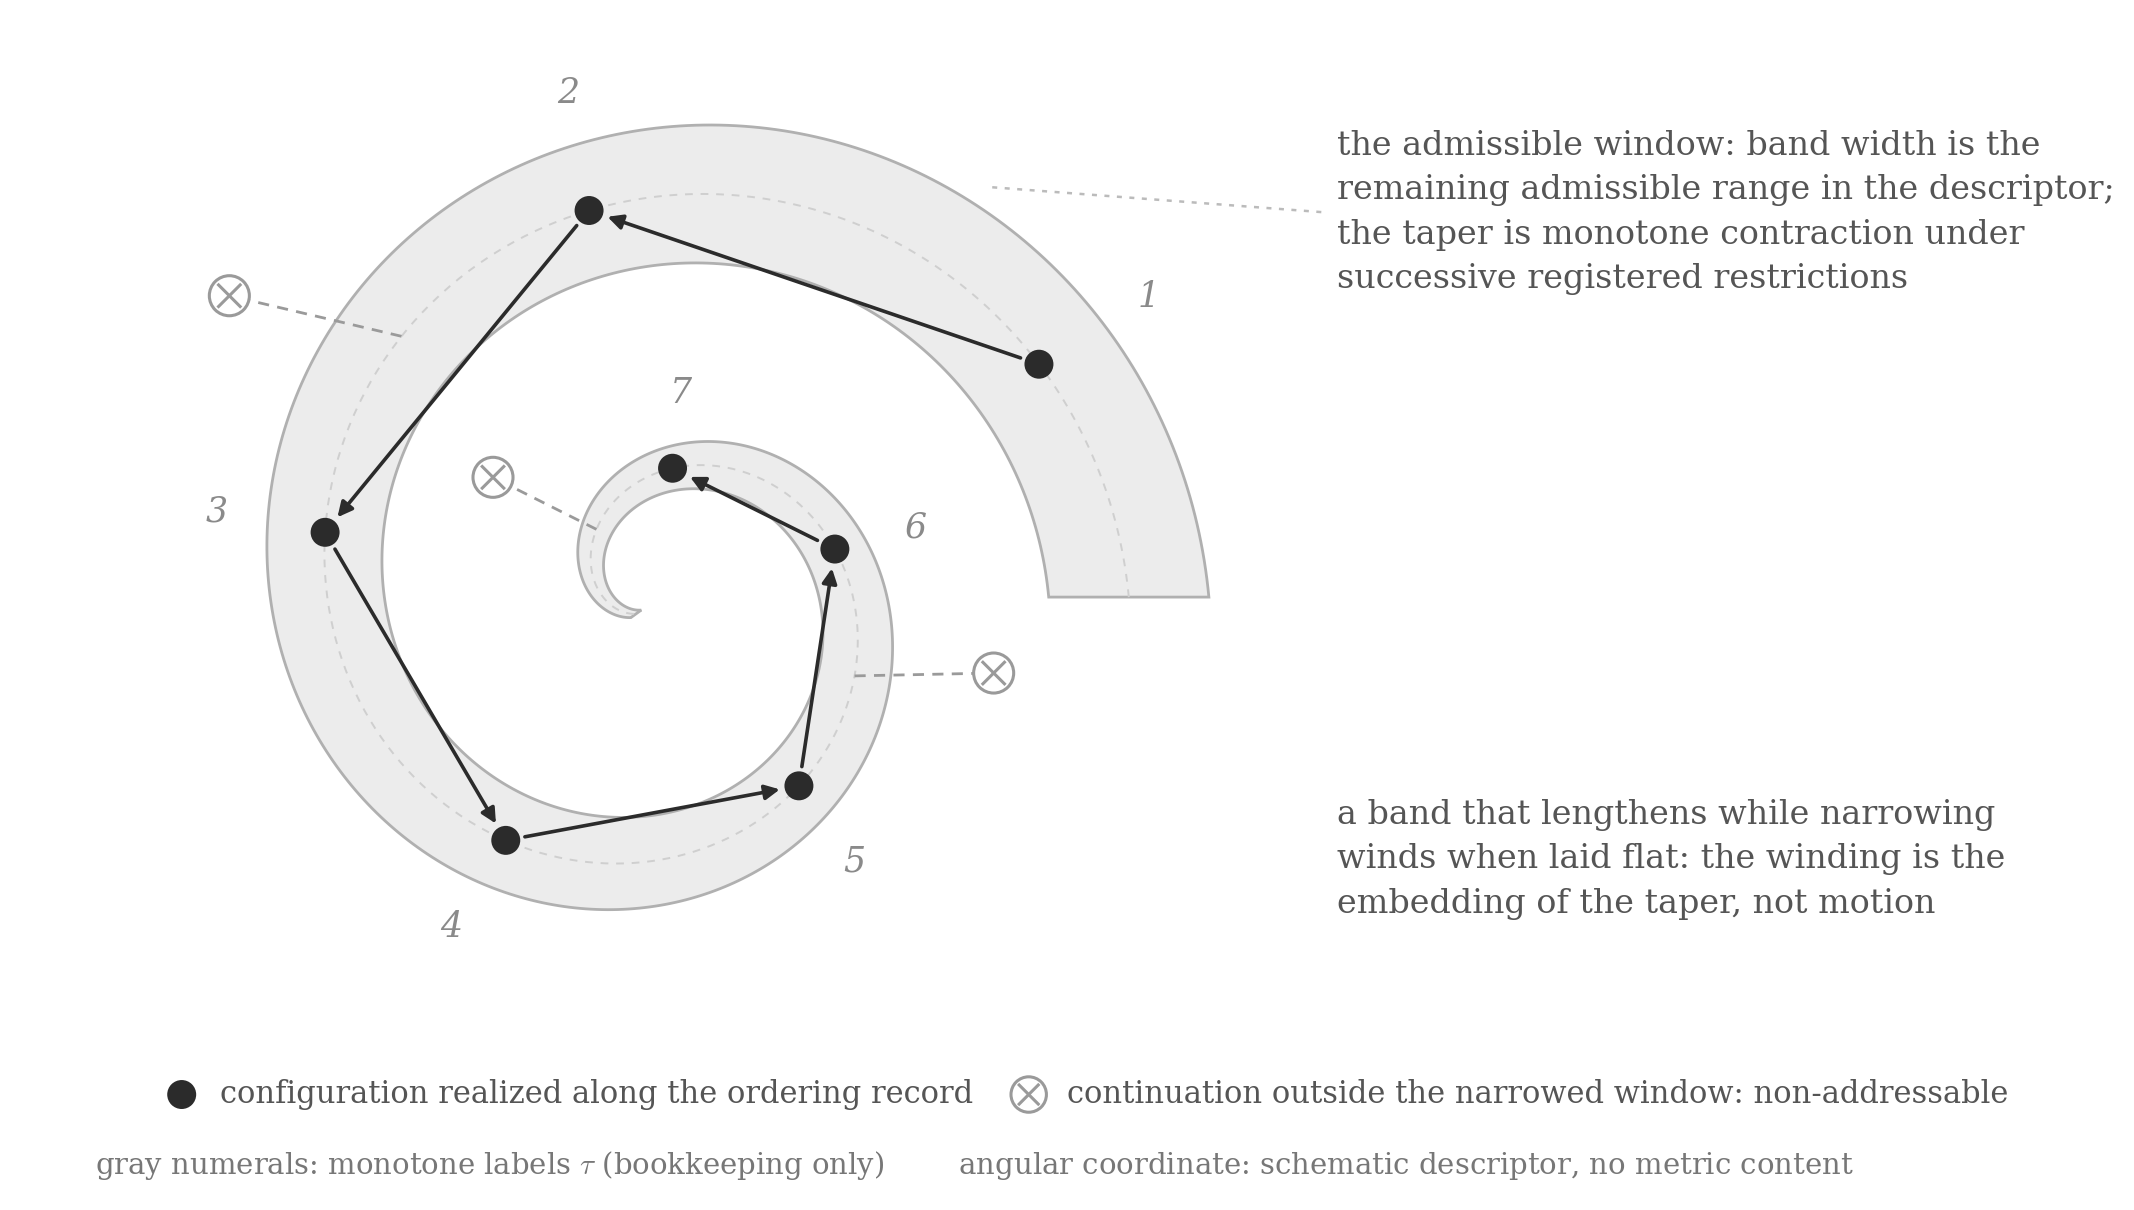
\includegraphics[width=0.75\linewidth]{admissible.png}
\captionsetup{justification=raggedright,singlelinecheck=false}
\caption{Sequencing as a tapering admissible band under fixed \(E\).
The angular coordinate is a schematic descriptor and carries no metric
content; band width is the remaining admissible window, and the taper
is monotone admissibility contraction under successive registered
restrictions. A band that lengthens while narrowing winds when laid
flat: the winding is the embedding of the taper, not motion. Black
arrows are realized ordering chains, prerequisite direction only; gray
numerals give a monotone labeling \(\tau\), bookkeeping only, as in
Fig.~\ref{fig:sequencing_partial_order}. Crossed stubs mark
continuations falling outside the narrowed window, non-addressable
relative to the realized record under the same \(E\). Dots encode
membership only and imply neither metric structure nor dynamics.}
\label{fig:admissibility_contraction_record}
\end{figure}

\subsection{Compatibility Envelopes and Closure}
\label{subsec:compatibility_envelopes}

\subsubsection{Compatibility predicate}
\label{subsubsec:compatibility_predicate}

Fix \(E\) and
\[
\mathcal{A}(E)\subseteq\Phi.
\]
Compatibility is represented by the pairwise predicate
\begin{equation}
\begin{aligned}
\mathrm{Compat}_E&:
\mathcal{A}(E)\times\mathcal{A}(E)
\to
\{0,1\},
\\
\mathrm{Compat}_E(\rho,\sigma)&=1
\;\Longleftrightarrow\;
\rho\text{ and }\sigma\text{ are pairwise compatible under }E.
\end{aligned}
\label{eq:compatibility_predicate}
\end{equation}

This is a pairwise coexistence predicate. It is not, by itself, a
connectivity relation, neighbourhood assignment, measure, topology, or
joint-consistency condition beyond the declared pair.

\subsubsection{Envelope representations}
\label{subsubsec:envelope_representation}

\paragraph{(i) Pair-envelope.}

The compatible pair set is
\begin{equation}
\mathcal{E}^{\mathrm{pair}}_E
:=
\{
(\rho,\sigma)\in
\mathcal{A}(E)\times\mathcal{A}(E):
\mathrm{Compat}_E(\rho,\sigma)=1
\}.
\label{eq:pair_envelope}
\end{equation}

This object records pairwise compatibility only. It does not determine
\(\Gamma_E\), \(\mathcal N_E\), or \(\mu_E\) unless a model-specific
construction explicitly identifies those structures.

\paragraph{(ii) Phase-offset envelope (model-dependent).}

When a model supplies a relational phase-offset map
\begin{equation}
\Delta\varphi_E:
\mathcal{A}(E)\times\mathcal{A}(E)
\to
S^1,
\label{eq:phase_offset_map_general}
\end{equation}
compatibility may be represented by a subset
\[
\mathcal{E}^{(\varphi)}_E\subseteq S^1
\]
such that
\begin{equation}
\mathrm{Compat}_E(\rho,\sigma)=1
\;\Longleftrightarrow\;
\Delta\varphi_E(\rho,\sigma)
\in
\mathcal{E}^{(\varphi)}_E.
\label{eq:phase_envelope_membership_general}
\end{equation}

The primitive content remains \(\mathrm{Compat}_E\). The phase-offset
form is a representational compression used only when
\(\Delta\varphi_E\) is explicitly supplied. It introduces no independent
phase space, Hamiltonian flow, topology, or dynamics.
Toy~\ref{toy:envelope_ordering} works a four-configuration
instance of this acceptance-window mechanism on \(S^1\).

\begin{proposition}[Equivalence of envelope representations]
\label{prop:envelope_rep_equiv}
Under the conditions of Eqs.~\eqref{eq:pair_envelope}
and~\eqref{eq:phase_envelope_membership_general}, for all
\[
\rho,\sigma\in\mathcal{A}(E),
\]
one has
\[
(\rho,\sigma)\in\mathcal{E}^{\mathrm{pair}}_E
\;\Longleftrightarrow\;
\Delta\varphi_E(\rho,\sigma)\in\mathcal{E}^{(\varphi)}_E.
\]
\end{proposition}

\begin{proof}
The claim follows directly by chaining the biconditionals in
Eqs.~\eqref{eq:pair_envelope}
and~\eqref{eq:phase_envelope_membership_general}.
\end{proof}

\subsubsection{Envelope closure and non-closure}
\label{subsubsec:envelope_nonclosure_structural}

Fix a representation space \(\Omega_E\) and a finite family
\[
\{\mathcal{E}^{(k)}_E\}_{k\in K},
\qquad
\mathcal{E}^{(k)}_E\subseteq\Omega_E.
\]
Define
\begin{equation}
\mathcal{E}^{(K)}_E
:=
\bigcap_{k\in K}
\mathcal{E}^{(k)}_E.
\label{eq:envelope_intersection}
\end{equation}

The family \emph{closes under \(E\)} if
\[
\mathcal{E}^{(K)}_E\neq\varnothing.
\]
Any element
\[
\omega\in\mathcal{E}^{(K)}_E
\]
is a \emph{closure witness}.

The family \emph{fails to close} if
\[
\mathcal{E}^{(K)}_E=\varnothing.
\]
In that case no witness satisfies all constraints simultaneously. This
is a structural domain-of-definition failure, not an epistemic
limitation, dynamical obstruction, or ontological boundary.

Envelope closure is a compatibility or constraint-satisfaction fact
under fixed \(E\), stated prior to any realized ordering record.
Within-ordering consequences for addressability are handled separately
with the ordering machinery
(Sec.~\ref{sec:structural_ordering_resolution}).

For a finite set
\[
\{\rho_i\}_{i\in V}
\]
with edge set
\[
\mathsf{E}\subseteq V\times V,
\]
a closure witness in pair/graph form is an assignment satisfying
\[
\mathrm{Compat}_E(\rho_i,\rho_j)=1
\]
for all
\[
(i,j)\in\mathsf{E}.
\]
This rendering does not assert that pairwise constraints exhaust joint
consistency unless a model supplies that reduction
\cite{Dechter2003}.

\subsection{Phase Compatibility Classes}
\label{subsec:phase_harmonics_ordering_struct}

``Harmonics'' in SSAF denotes phase-compatibility class structure under
fixed \(E\): (i) \emph{signature classes} defined by unary
constraint-membership profiles on \(\mathcal{A}(E)\), and (ii)
\emph{compatibility classes} defined as maximal pairwise compatible
sectors under \(\mathrm{Compat}_E\).

No spectral, Fourier, eigenmode, frequency, or dynamical meaning is
implied. ``Harmonics'' refers to hierarchical repetition of
compatibility patterns across descriptive resolution, not oscillatory
dynamics or frequency spectra.

The constructions below are classification structures. They do not
define \(\Gamma_E\), \(\mathcal N_E\), \(\mu_E\), sequencing, topology,
or dynamics unless a model-specific construction explicitly identifies
those objects.

\paragraph{Unary constraint vocabulary.}

Fix \(E\) and a finite family
\[
\{U^{(k)}_E\}_{k\in K}
\]
with
\[
U^{(k)}_E\subseteq\mathcal{A}(E)\subseteq\Phi.
\]
Each \(U^{(k)}_E\) is used only for membership tests; no updating rule,
dynamics, connectivity relation, neighbourhood assignment, or measure is
introduced.

\paragraph{Constraint-membership profile.}

Define
\begin{equation}
\mathbf{s}_E :
\mathcal{A}(E)
\to
\{0,1\}^K,
\qquad
\mathbf{s}_E(\rho)_k
:=
\mathbf{1}\{\rho\in U^{(k)}_E\}.
\label{eq:constraint_profile_map_struct}
\end{equation}

\paragraph{Signature classes.}

Define
\[
\rho\equiv_E\sigma
\quad\Longleftrightarrow\quad
\mathbf{s}_E(\rho)=\mathbf{s}_E(\sigma).
\]
A \emph{signature class}
\[
\mathcal{S}_i(E)\subseteq\mathcal{A}(E)
\]
is an equivalence class under \(\equiv_E\).

The vector \(\mathbf{s}_E(\rho)\) is the \emph{constraint signature} of
\(\rho\): a constraint-satisfaction profile, not a phase estimator,
dynamical label, or update parameter.

\begin{lemma}[Signature classes form a partition]
\label{lem:signature_partition}
\(\equiv_E\) is an equivalence relation on \(\mathcal{A}(E)\); the
family \(\{\mathcal{S}_i(E)\}\) partitions \(\mathcal{A}(E)\).
\end{lemma}

\begin{proof}
Reflexivity, symmetry, and transitivity follow from equality of profile
vectors.
\end{proof}

\paragraph{Constraint-inclusion order.}

For
\[
\mathbf{s},\mathbf{s}'\in\{0,1\}^K,
\]
define
\[
\mathbf{s}\preceq\mathbf{s}'
\quad\Longleftrightarrow\quad
\mathbf{s}_k\leq\mathbf{s}'_k
\quad
\text{for all }k\in K.
\]

This compares constraint-satisfaction strength only and introduces no
sequencing, dynamics, metric, or temporal order.

\begin{lemma}[Signature poset]
\label{lem:signature_poset}
\(\preceq\) is a partial order on \(\{0,1\}^K\).
\end{lemma}

\begin{proof}
Reflexivity, antisymmetry, and transitivity hold coordinatewise.
\end{proof}

\paragraph{Induced order on signature classes.}

For signature classes \(\mathcal{S}\) and \(\mathcal{S}'\), define
\[
\mathcal{S}\preceq\mathcal{S}'
\]
if
\[
\mathbf{s}_E(\rho)\preceq\mathbf{s}_E(\sigma)
\]
for any
\[
\rho\in\mathcal{S},
\qquad
\sigma\in\mathcal{S}'.
\]

\begin{lemma}[Well-defined class order]
\label{lem:class_order_welldefined}
The induced \(\preceq\) on signature classes is well-defined and
inherits the partial-order structure from \(\{0,1\}^K\).
\end{lemma}

\begin{proof}
All elements of a class share the same profile by definition of
\(\equiv_E\), so the comparison is representative-independent.
\end{proof}

\paragraph{Compatibility classes.}

Fix \(E\) and \(\mathcal{A}(E)\), and suppose a symmetric
compatibility relation is available for the construction. A
\emph{compatibility class} is a maximal subset
\[
\mathcal{K}\subseteq\mathcal{A}(E)
\]
such that
\[
\mathrm{Compat}_E(\rho,\sigma)=1
\]
for all distinct
\[
\rho,\sigma\in\mathcal{K}.
\]

Equivalently, when \(\mathrm{Compat}_E\) is symmetric, compatibility
classes are maximal cliques of the graph on \(\mathcal{A}(E)\) with
edges where \(\mathrm{Compat}_E=1\).

No partition, uniqueness, connected-component structure,
neighbourhood structure, measure, topology, or sequencing relation is
implied.

\paragraph{Constraint-refined domain (optional).}

Define the optional constraint-refined admissible domain
\[
\mathcal{A}_K(E)
:=
\mathcal{A}(E)
\cap
\bigcap_{k\in K}U^{(k)}_E.
\]

Compatibility classes may then be defined as maximal pairwise
compatible subsets of \(\mathcal{A}_K(E)\).

If \(\mathrm{Compat}_E\) is not symmetric, class formation may use the
symmetric part of the predicate, so that \(\rho\) and \(\sigma\) count
as compatible for class construction only when
\[
\mathrm{Compat}_E(\rho,\sigma)
=
\mathrm{Compat}_E(\sigma,\rho)
=
1.
\]

This symmetrization is local to class formation and does not alter
\(\mathrm{Compat}_E\) elsewhere. Class membership is representational
only. A finite instance exercising this classification vocabulary,
with explicit signature classes and their induced order, is worked in
Toy~\ref{toy:harmonics_instance}.

\subsection{Permissible Structures as Constraint Closure}
\label{subsec:permissible_structure_struct}

Within fixed \(E\), a pattern is a \emph{permissible structure} when its
defining \(E\)-indexed constraints admit at least one licensed witness,
i.e.\ when the stated constraint family closes
(Sec.~\ref{subsubsec:envelope_nonclosure_structural}).

Compatibility closure is one important case of permissible structure,
but it is not the only one. The construction below is typed so that
compatibility constraints, joint-admissibility constraints, interface
constraints, and other explicitly declared \(E\)-indexed constraint
families can be treated without confusing their roles.

\subsubsection{Typing discipline}
\label{subsubsec:permissible_structure_typing}

Fix \(E\). Let \(\mathsf{W}_E\) denote the witness space and
\(\mathsf{X}_E\) the target configuration space:
\[
\mathsf{W}_E
\in
\{
\mathcal{A}(E),\;
\mathcal{A}(E)\times\mathcal{A}(E),\;
\Phi_A\times\Phi_B,\;
\Phi_{AB},\;
\ldots
\},
\]
and
\[
\mathsf{X}_E
\in
\{
\Phi,\;
\Phi_A,\;
\Phi_B,\;
\Phi_{AB},\;
\ldots
\}.
\]

Let
\[
\mathcal{A}^{\mathrm{tgt}}(E)
\subseteq
\mathsf{X}_E
\]
be the admissible target set.

A constraint family is represented as subsets
\[
\{\mathcal{E}^{(k)}_E\}_{k\in K},
\qquad
\mathcal{E}^{(k)}_E\subseteq\mathsf{W}_E,
\]
with intersection envelope
\begin{equation}
\mathcal{E}^{(K)}_E
:=
\bigcap_{k\in K}
\mathcal{E}^{(k)}_E
\subseteq
\mathsf{W}_E.
\label{eq:permissible_structure_intersection_envelope}
\end{equation}

When
\[
\mathsf{W}_E\neq\mathsf{X}_E,
\]
configuration-level satisfaction requires an explicit witnessing
convention via a projection or interpretation map
\[
\pi_E:\mathsf{W}_E\to\mathsf{X}_E.
\]

Then
\begin{equation}
x\models_E k
\;\Longleftrightarrow\;
\exists\,w\in\mathcal{E}^{(k)}_E
\quad
\text{with}
\quad
\pi_E(w)=x.
\label{eq:permissible_structure_witnessing_convention}
\end{equation}

For example, in a pair-witness representation one may use
\[
\pi_E(\rho,\sigma)=\rho,
\]
while in a joint-state representation one may use
\[
\pi_E(\rho_{AB})=\rho_{AB}.
\]

The map \(\pi_E\) is bookkeeping only. It is not a dynamical map, update
rule, measurement map, connectivity relation, neighbourhood assignment,
or admissibility measure.

\subsubsection{Definition: permissible structure}
\label{subsubsec:permissible_structure_def_struct}

Fix \(E\), \(\mathsf{W}_E\), \(\mathsf{X}_E\),
\(\mathcal{A}^{\mathrm{tgt}}(E)\), and a finite constraint family
\[
\{\mathcal{E}^{(k)}_E\}_{k\in K}.
\]

The associated \emph{permissible structure under \(E\)} is
\begin{equation}
\mathcal{S}^{(K)}_E
:=
\pi_E\bigl(\mathcal{E}^{(K)}_E\bigr)
\cap
\mathcal{A}^{\mathrm{tgt}}(E)
\subseteq
\mathcal{A}^{\mathrm{tgt}}(E).
\label{eq:permissible_structure_set_def}
\end{equation}

The pattern is \emph{permissible} if the constraint family closes:
\begin{equation}
\mathcal{E}^{(K)}_E
\neq
\varnothing.
\label{eq:permissible_structure_closure}
\end{equation}

When the closure condition holds and \(\pi_E\) is defined on
\(\mathcal{E}^{(K)}_E\), the projected permissible structure
\(\mathcal{S}^{(K)}_E\) is defined. If the projected set is empty after
intersection with \(\mathcal{A}^{\mathrm{tgt}}(E)\), then the witness
constraints close in \(\mathsf{W}_E\) but do not license a target-level
structure in \(\mathsf{X}_E\).

The boundary is a domain-of-definition boundary, not a spatial surface.

When constraints are represented by \(\mathrm{Compat}_E\), and when a
model licenses reduction of joint feasibility to pairwise tests,
permissible structure may be rendered as a compatibility-closed sector
in the pair-envelope graph
(Eq.~\ref{eq:pair_envelope}).

This rendering does not assert
\[
\text{pairwise closure}
\Longrightarrow
\text{joint closure}
\]
unless the model supplies that equivalence~\cite{Dechter2003,Diestel2017}.

A permissible structure is not automatically a connected component of
\(\Gamma_E\), a neighbourhood under \(\mathcal N_E\), a basin, a
topological region, or a measured region under \(\mu_E\). Those
identifications require explicit model-specific assumptions.

\subsubsection{Constraint geometry}
\label{subsubsec:constraint_geometry_compat_struct}

Admissibility and compatibility constraints delimit relational
organization under fixed \(E\) by excluding assignments for which the
required constraint family fails to close, witnessed by envelope
non-closure
(Sec.~\ref{subsubsec:envelope_nonclosure_structural}).

In reconstructions this may appear anisotropic, geometric, or
topologically constrained. The structural content is only the closure
criterion
\[
\mathcal{E}^{(K)}_E\neq\varnothing
\]
together with the induced domain-of-definition boundary.

Any geometric, topological, connectivity, neighbourhood, or
measure-theoretic interpretation must be supplied by the model and is
not implied by constraint closure alone.

\subsection{Phase Locking, Drift, and Closure Language}
\label{subsec:phase_locking_drift_struct}

``Locking'' and ``drift'' are representational shorthand for closure or
failure of closure of a stated \(E\)-indexed constraint vocabulary. No
dynamical mechanism, force law, relaxation process, or phase-flow
mechanism is implied.

Fix \(E\), a finite constraint vocabulary \(K\), and a witness space
\(\Omega_E\) with
\[
\mathcal{E}^{(k)}_E\subseteq\Omega_E
\]
for each \(k\in K\). Define
\begin{equation}
\mathcal{E}^{(K)}_E
:=
\bigcap_{k\in K}
\mathcal{E}^{(k)}_E
\subseteq
\Omega_E.
\label{eq:locking_intersection_envelope}
\end{equation}

The vocabulary is \emph{locked} if
\begin{equation}
\mathcal{E}^{(K)}_E
\neq
\varnothing,
\label{eq:locking_closure_nonempty}
\end{equation}
and \emph{drifts} if
\begin{equation}
\mathcal{E}^{(K)}_E
=
\varnothing.
\label{eq:drift_nonclosure_empty}
\end{equation}

Thus locking means that at least one witness satisfies all stated
constraints simultaneously. Drift means that no such witness exists
within the declared \(E\)-indexed domain.

Drift is a domain-of-definition failure, not an epistemic limitation,
dynamical instability, or ontological removal from \(\Phi\).

When the envelope representation is not unary, configuration-level
statements require an explicit projection or interpretation map
\[
\pi_E:\Omega_E\to\mathsf{X}_E.
\]
Then
\begin{equation}
x\models_E k
\;\Longleftrightarrow\;
\exists\,w\in\mathcal{E}^{(k)}_E
\quad
\text{with}
\quad
\pi_E(w)=x.
\label{eq:witness_projection_general_to_target}
\end{equation}

The projection \(\pi_E\) is bookkeeping only. It is not a dynamical map,
update rule, measurement operation, connectivity relation, neighbourhood
assignment, or admissibility measure.

Locking and drift language does not define \(\Gamma_E\),
\(\mathcal N_E\), or \(\mu_E\). Those structures may be used to analyze
the organization of a locked or drifting constraint family only when a
model-specific construction explicitly supplies that connection.

\subsubsection{Non-permissible configurations}
\label{subsubsec:nonpermissible_configurations_phase_struct}

Patterns whose constraint vocabulary fails to close under fixed \(E\)
are not permissible structures within that \(E\)-indexed domain
(Sec.~\ref{subsubsec:permissible_structure_def_struct}).

They may appear in coarse reconstructions after quotienting by
\(\sim_E\), but they fail licensing as a matter of constraint
non-closure, not because any element is removed from \(\Phi\).

A non-permissible pattern is therefore not forbidden, destroyed, or
dynamically blocked. It is simply outside the domain on which the
declared constraint vocabulary supports a well-defined permissible
structure under fixed \(E\).

\subsection{Phase Locality}
\label{subsec:phase_locality_struct}

Locality is a context-indexed notion internal to admissible structure,
not separation in a background spatial manifold.

Fix \(E\) and suppose a model supplies a phase-sensitive separation
function
\[
d_\Phi:\Phi\times\Phi\to\mathbb R_{\geq 0},
\]
such as the Bures metric on density operators or the Fubini--Study
metric on pure-state charts~\cite{BengtssonZyczkowski2006,
NielsenChuang2010,Watrous2018}.

Define a context-locality scale
\[
d_{\mathrm{loc}}(E)\geq 0
\]
and the corresponding phase-local ball
\begin{equation}
\mathcal B_E^{\mathrm{loc}}(\rho)
:=
\{
\sigma\in\mathcal A(E):
d_\Phi(\rho,\sigma)\leq d_{\mathrm{loc}}(E)
\}.
\label{eq:phase_local_ball_struct}
\end{equation}

The scale \(d_{\mathrm{loc}}(E)\) is indexed only by \(E\). It may not
depend on \(\rho\), outcomes, ensemble decompositions, or any
state-derived diagnostic, in accordance with NS1.

The object \(\mathcal B_E^{\mathrm{loc}}(\rho)\) is a
model-specific locality witness. It is not the derived neighbourhood
\(\mathcal N_E(\rho)\) unless a model explicitly identifies
\[
\mathcal N_E(\rho)
=
\mathcal B_E^{\mathrm{loc}}(\rho).
\]

A cross-configuration comparison is well-posed only when the relevant
witness or envelope constraints admit closure after restriction to the
declared locality witness. Otherwise the comparison is undefined
(Sec.~\ref{subsubsec:envelope_nonclosure_structural}).

No background spatial locality, metric geometry, topology, or dynamical
propagation is implied.

\subsection{Non-Uniqueness and Admissibility Width}
\label{subsec:admissibility_width_struct}

\begin{definition}[Admissibility width]
\label{def:admissibility_width}
Fix \(E\). The admissible description has \emph{nontrivial
admissibility width} if
\begin{equation}
\exists\,\rho,\sigma\in\mathcal A(E)
\quad\text{with}\quad
\rho\neq\sigma.
\label{eq:admissibility_width_nontrivial}
\end{equation}
\end{definition}

Admissibility width introduces no probability measure, sampling rule,
aggregation principle, connectivity relation, neighbourhood assignment,
or admissibility measure~\cite{NielsenChuang2010,Watrous2018}.

It is independent of closure: a permissible structure may have internal
width, meaning multiple distinct witnesses may remain consistent with
fixed \(E\).

In basin-style descriptions, two structural failure modes arise:

\begin{enumerate}[label=(\roman*), leftmargin=2.2em]

\item \emph{Underconstrained structure:} the constraints are too weak to
delimit a boundary-defined unit.

\item \emph{Inconsistent structure:} no simultaneous witness exists
under fixed \(E\), corresponding to envelope non-closure.

\end{enumerate}

A basin description is well-posed only when the defining constraint
family admits closure under \(E\)
(Sec.~\ref{subsec:permissible_structure_struct}).

A basin is not automatically a connected component of \(\Gamma_E\), a
neighbourhood under \(\mathcal N_E\), a topological region, or a
measured region under \(\mu_E\). Those identifications require explicit
model-specific assumptions.

\subsection{Projection Effects and Apparent Geometry}
\label{subsec:projection_effects_geometry_struct}

Within envelope-closed domains under fixed \(E\), compatibility-closed
or constraint-closed structure may admit effective representations
resembling rings, spirals, shells, networks, or other geometric forms.

In SSAF these are projection effects: embeddings, cross-sections, or
visual compressions of admissible structure in \(\Phi\).

Any observed regularity is representational, choice-dependent, and
context-dependent~\cite{BengtssonZyczkowski2006,Paris2009,Watrous2018}.

Projection geometry does not by itself define \(\Gamma_E\),
\(\mathcal N_E\), \(\mu_E\), topology, metric structure, sequencing, or
dynamics. Those structures must be declared explicitly when used.

\subsection{Low-Constraint Regimes and Effective Flat Geometry}
\label{subsec:low_constraint_flat_geometry_struct}

Low-constraint regimes correspond to contexts \(E\) in which the
induced admissibility and structural organization is weakly articulated,
and closure-supported landmarks are sparse or absent. When such
landmarks are absent, reconstruction-level diagnostics admit no robust
curvature, anisotropy, localization, connectivity, or concentration
descriptors.

``Flat'' geometry denotes absence of closure-supported structure for the
chosen reconstruction under fixed \(E\), not ontological emptiness of
\(\Phi\), and not absence of admissible configurations
\cite{Peebles2001,BondKofmanPogosyan1996,Sheth2004,vanDeWeygaert2011}.

\subsection{Limits of Geometric Reconstruction}
\label{subsec:limits_reconstruction_struct}

Geometric descriptions are emergent mappings of admissible structure,
not structural primitives. Distinct admissibility or structural regimes
may project to geometrically indistinguishable descriptions under all
accessible \(\mathcal{O}(E)\), while similar constraints may admit
divergent geometric renderings depending on coarse-graining, feature
selection, connectivity choices, neighbourhood assignments, or measure
choices.

SSAF does not assert recoverability between admissibility structure and
any geometric representation~\cite{Wald1984,ButterfieldIsham2001}.

\subsection{Closing Link}
\label{subsec:closing_link_phase_ordering_struct}

Structure arises when a phase-relational pattern forms a
constraint-closed unit under fixed \(E\)
(Sec.~\ref{subsec:permissible_structure_struct}). Compatibility closure
is one important case, but other \(E\)-indexed constraint families may
also support permissible structure.

Patterns that fail closure remain elements of \(\Phi\), when their
configurations are elements of \(\Phi\), but they do not define
boundary-robust units of description within that fixed context.

Consequences for environment-driven restriction, non-addressability, and
irreversible sequencing are treated in
Sec.~\ref{sec:structural_ordering_resolution}.

\section{Structural Consequences of Ordering-Based Resolution}
\label{sec:structural_ordering_resolution}

Under fixed \(E\), resolution is restriction of which distinctions
remain addressable within a realized ordering. No configuration is
created, destroyed, or retroactively modified. When updating is
represented, it uses linear CPTP maps consistent with
NS1~\cite{Kraus1983,NielsenChuang2010,Watrous2018}.

Joint-admissibility structure, compatibility structure, connectivity
structure, neighbourhood structure, and admissibility measure are fixed
upstream in Core Definitions and Structural Primitives. Nothing here
alters those objects.

\subsection{Basin Vocabulary}
\label{subsec:ordering_resolution_scope}

Basin language denotes admissibility and structural organization in
\(\Phi\) under fixed \(E\), used only as representational compression
with no dynamical content.

Basin vocabulary here is restricted to unary constraint vocabularies
\[
\{\mathcal{E}^{(k)}_E\subseteq\mathcal{A}(E)\}_{k\in K}
\]
together with the derived neighbourhood structure. Pair and joint
envelopes are handled upstream
(Sec.~\ref{subsec:permissible_structure_struct}).

\begin{definition}[Coherence basin]
\label{def:coherence_basin_struct}
Fix \(E\), a unary constraint vocabulary
\[
\{\mathcal{E}^{(k)}_E\}_{k\in K},
\]
and the connectivity structure \(\Gamma_E\), which fixes the derived
neighbourhood assignment
\[
\mathcal N_E(\rho)=\{\sigma\in\mathcal A(E):(\rho,\sigma)\in\mathcal R_E\}.
\]

A \emph{coherence basin} is any nonempty subset
\[
\mathcal{B}\subseteq\mathcal{A}(E)
\]
such that for every
\[
\rho\in\mathcal{B},
\]
one has
\begin{equation}
\bigcap_{k\in K}
\bigl(
\mathcal{E}^{(k)}_E
\cap
\mathcal{N}_E(\rho)
\bigr)
\neq
\varnothing.
\label{eq:basin_local_closure}
\end{equation}

This is a local closure condition inside the derived neighbourhood
structure. It introduces no flow, update rule, force law, potential, or
basin dynamics.
\end{definition}

A coherence basin is not automatically a topological basin, metric
ball, attractor basin, connected component of \(\Gamma_E\), or measured
region under \(\mu_E\). Those identifications require explicit
model-specific assumptions. A scalar depth functional realizing
monotone basin descent under admissible updating is constructed in
Toy~\ref{toy:coherence_basin_depth_functional_contraction}.

\begin{definition}[Coherence margin]
\label{def:coherence_margin_struct}
The \emph{coherence margin} of \(\mathcal{B}\) is the set of
\[
\rho\in\mathcal{A}(E)
\]
for which local closure
\eqref{eq:basin_local_closure} holds for some interface scales but fails
for others at fixed \(E\).

Closure sensitivity here is a reconstruction or structural-assignment
sensitivity, not a dynamical instability.
\end{definition}

\begin{definition}[Microbasin]
\label{def:microbasin_struct}
A \emph{microbasin} is a basin-like set \(\mathcal{B}\) for which local
closure holds only in a regime that fails under modest coarsening of the
interface or tightening of the constraint vocabulary.

This is a threshold classification, not a dynamical claim.
\end{definition}

\subsection{Resolution as Restriction of Addressability}
\label{subsec:resolution_as_restriction}

A restriction step is \emph{registered} within a realized ordering
under fixed \(E\) when a protocol-defined descriptor exists whose
\(\sim_E\)-equivalence class remains stable under repeated admissible
use of the same interface within \(E\)
(cf.~Theorem~\ref{thm:fixed_context_no_retro_addressability}).

\begin{proposition}[Registered restriction yields terminal non-addressability]
\label{prop:registered_implies_terminal_nonaddr}
Fix \(E\) with \((\mathrm{IC}_E)\). If a restriction is registered as a
stable \(\sim_E\)-class record within a realized ordering, then any
distinction excluded by that restriction is non-addressable within the
same ordering: no admissible in-domain operation under fixed \(E\)
restores, queries, or conditions on the excluded distinction.
\end{proposition}

\begin{proof}
By \((\mathrm{IC}_E)\) and
Theorem~\ref{thm:fixed_context_no_retro_addressability}, every
admissible in-domain CPTP update preserves \(\sim_E\). Restoring an
excluded distinction would require refining
\[
\Phi/{\sim_E},
\]
which no admissible in-domain operation under fixed \(E\) licenses.
\end{proof}

\subsubsection{Sequencing as acyclic restriction}
\label{subsec:sequencing_as_restriction}

\begin{theorem}[Sequencing induces a strict partial order]
\label{thm:sequencing_strict_partial_order}
Fix \(E\). For registered restriction steps \(r\) within a realized
ordering, let \(\mathsf{Addr}_E(r)\) denote the set of addressable
distinctions after step \(r\). Define
\[
r_1\prec_E r_2
\;\Longleftrightarrow\;
\mathsf{Addr}_E(r_2)
\subsetneq
\mathsf{Addr}_E(r_1).
\]
Then \(\prec_E\) is a strict partial order admitting no cycles.
\end{theorem}

\begin{proof}
Irreflexivity holds because no set is a strict subset of itself.
Transitivity holds because strict set inclusion is transitive. A cycle
would imply a strict inclusion chain from a set into itself, which is
impossible.
\end{proof}

\subsubsection{Envelope non-closure as terminality}
\label{subsec:envelope_nonclosure_terminality}

\begin{proposition}[Envelope non-closure yields terminal non-addressability]
\label{prop:nonclosure_implies_terminal_nonaddr}
Fix \(E\) and a finite family
\[
\{\mathcal{E}^{(k)}_E\}_{k\in K},
\qquad
\mathcal{E}^{(k)}_E\subseteq\Omega_E.
\]
If
\[
\mathcal{E}^{(K)}_E
:=
\bigcap_{k\in K}
\mathcal{E}^{(k)}_E
=
\varnothing,
\]
then:
\begin{enumerate}[label=(\roman*), leftmargin=2.2em]
\item no closure witness exists under fixed \(E\);
\item any claim requiring such a witness is \emph{undefined} in the
fixed-\(E\) description and cannot be registered as an addressable
distinction in any realized ordering under \(E\).
\end{enumerate}
\end{proposition}

\begin{proof}
Item (i) is immediate from emptiness. For (ii), the witness-existence
precondition fails under fixed \(E\), so the claim is undefined. Since
registered addressability applies only to licensed distinctions, the
non-closing comparison cannot be registered under any realized ordering
at fixed \(E\).
\end{proof}

\subsection{Restriction Nesting and Persistence Classes}
\label{subsec:restriction_nesting_persistence_struct}

Fix \(E\). Context-indexed restriction is represented by a nested family
\[
\widetilde{\mathcal{A}}_0(E)
\supseteq
\widetilde{\mathcal{A}}_1(E)
\supseteq
\widetilde{\mathcal{A}}_2(E)
\supseteq
\cdots,
\qquad
\widetilde{\mathcal{A}}_0(E):=\mathcal{A}(E).
\]

\begin{definition}[Persistence class]
\label{def:persistence_class_struct}
Fix \(E\), the nesting above, and a regime index set
\[
\mathsf{R}\subseteq\mathbb{N}.
\]
A \emph{persistence class} is a nonempty subset
\[
\mathcal{P}\subseteq\mathcal{A}(E)
\]
satisfying:
\begin{enumerate}[label=(\roman*), leftmargin=2.2em]

\item \textbf{Closure:}
\(\mathcal{P}\) is constraint-closed under \(E\)
(Sec.~\ref{subsubsec:permissible_structure_def_struct}).

\item \textbf{Regime persistence:}
there exists
\[
N\in\mathbb{N}\cup\{+\infty\}
\]
with
\[
\mathsf{R}=\{0,\ldots,N\}
\]
and
\[
\mathcal{P}\cap\widetilde{\mathcal{A}}_n(E)\neq\varnothing
\]
for all \(n\in\mathsf{R}\).

\item \textbf{Signature stability:}
the defining envelope constraints of \(\mathcal{P}\) continue to admit
closure witnesses on \(\mathsf{R}\).

\end{enumerate}
\end{definition}

Define the addressable first-exclusion index
\[
\widetilde{k}_{\mathrm{ex}}(\rho)
:=
\inf
\{
n\geq 0:
\rho\notin\widetilde{\mathcal{A}}_n(E)
\},
\]
with
\[
\widetilde{k}_{\mathrm{ex}}(\rho)=+\infty
\]
if \(\rho\) persists throughout.

\begin{proposition}[Persistence implies late exclusion]
\label{prop:persistence_implies_late_exclusion}
Let \(\mathcal{P}\) be a persistence class over
\[
\mathsf{R}=\{0,\ldots,N\}.
\]
Then there exists
\[
\rho\in\mathcal{P}
\]
with
\[
\rho\in\widetilde{\mathcal{A}}_n(E)
\]
for all \(n\in\mathsf{R}\), so
\[
\widetilde{k}_{\mathrm{ex}}(\rho)>N.
\]
\end{proposition}

\begin{proof}
By regime persistence, choose
\[
\rho\in
\mathcal{P}\cap\widetilde{\mathcal{A}}_N(E).
\]
Since the nesting is decreasing,
\[
\widetilde{\mathcal{A}}_N(E)
\subseteq
\widetilde{\mathcal{A}}_n(E)
\]
for all \(n\leq N\). Therefore
\[
\rho\in\widetilde{\mathcal{A}}_n(E)
\]
for all \(n\in\mathsf{R}\).
\end{proof}

\subsection{Axiom Unit Test: Ordering Density from Admissible-Set Restriction}
\label{subsec:ordering_density_unit_test}

\paragraph{What this unit test shows.}

This unit test introduces an ordering-density diagnostic derived from
successive restrictions of admissible sets under fixed context \(E\).
The diagnostic measures how much admissible structure is excluded from
the continuing admissible domain across a declared sequencing window.
Configurations persisting across the whole window are characterized by
Proposition~\ref{prop:persistence_implies_late_exclusion}.

It is not a primitive, not a time density, not a dynamical rate, not a
measure of physical duration, and not a modification of CPTP updating.

\paragraph{Setup.}

Fix a classical context \(E\). Let
\[
\mathcal A(E)
=
\mathcal A_0(E)
\supseteq
\mathcal A_1(E)
\supseteq
\cdots
\supseteq
\mathcal A_n(E)
\]
be a finite admissible-set restriction chain associated with a realized
sequencing record.

Each inclusion represents loss of addressability or restriction of the
in-domain claim set under the same fixed context. No element of \(\Phi\)
is destroyed or removed from the ambient configuration space.

Assume the admissibility measure \(\mu_E\) is defined on the relevant
subsets and is monotone:
\[
U\subseteq V\subseteq \mathcal A(E)
\quad\Longrightarrow\quad
\mu_E(U)\leq \mu_E(V).
\]

\paragraph{Resolved admissibility over a step.}

For each step \(i\to i+1\), define the resolved admissibility content
\[
\Delta_E^{\mathrm{ord}}(i)
:=
\mu_E\!\left(\mathcal A_i(E)\right)
-
\mu_E\!\left(\mathcal A_{i+1}(E)\right).
\]

By monotonicity,
\[
\Delta_E^{\mathrm{ord}}(i)\geq 0.
\]

\paragraph{Ordering density over a finite window.}

For a finite sequencing window
\[
W=[i,j],
\qquad
0\leq i<j\leq n,
\]
define the ordering-density diagnostic
\begin{equation}
\delta_E^{\mathrm{ord}}(W)
:=
\frac{
\mu_E\!\left(\mathcal A_i(E)\right)
-
\mu_E\!\left(\mathcal A_j(E)\right)
}{
j-i
}.
\label{eq:ordering_density_window}
\end{equation}

Equivalently,
\[
\delta_E^{\mathrm{ord}}(W)
=
\frac{1}{j-i}
\sum_{\ell=i}^{j-1}
\Delta_E^{\mathrm{ord}}(\ell).
\]

Thus \(\delta_E^{\mathrm{ord}}(W)\) is the average admissible-set
restriction per sequencing step across the chosen window.

\paragraph{Normalized ordering density.}

When
\[
\mu_E(\mathcal A_i(E))>0,
\]
define the normalized diagnostic
\begin{equation}
\widehat{\delta}_E^{\mathrm{ord}}(W)
:=
\frac{
\mu_E\!\left(\mathcal A_i(E)\right)
-
\mu_E\!\left(\mathcal A_j(E)\right)
}{
\mu_E\!\left(\mathcal A_i(E)\right)
}.
\label{eq:ordering_density_normalized}
\end{equation}

This gives the fraction of initially admissible structure excluded from
the continuing admissible domain over the window. By monotonicity,
\[
0
\leq
\widehat{\delta}_E^{\mathrm{ord}}(W)
\leq
1.
\]

\paragraph{Unit-test consequences.}

The diagnostic has three immediate consequences.

First, if no admissible-set restriction occurs over the window, then
\[
\mathcal A_i(E)=\mathcal A_j(E)
\quad\Longrightarrow\quad
\delta_E^{\mathrm{ord}}(W)=0.
\]

Second, if the admissible domain strictly contracts over the window and
\[
\mu_E\!\left(\mathcal A_i(E)\right)
>
\mu_E\!\left(\mathcal A_j(E)\right),
\]
then
\[
\delta_E^{\mathrm{ord}}(W)>0.
\]

Third, if a proposed sequencing record requires
\[
\mu_E\!\left(\mathcal A_{i+1}(E)\right)
>
\mu_E\!\left(\mathcal A_i(E)\right)
\]
under fixed \(E\), then the record is not an admissible restriction
chain. It represents context re-indexing, reconstruction change, or
external enlargement of the admissible domain, not fixed-context
sequencing.

\paragraph{NS1 hygiene.}

The quantities
\[
\Delta_E^{\mathrm{ord}}(i),
\qquad
\delta_E^{\mathrm{ord}}(W),
\qquad
\widehat{\delta}_E^{\mathrm{ord}}(W)
\]
are diagnostics only. They do not determine update maps, select
generators, alter admissibility, retune \(\Gamma_E\), reassign
\(\mathcal N_E\), reweight \(\mu_E\), or set resolution rates.

All dependence is through the fixed context \(E\), the declared
admissible-set chain, and the structural measure \(\mu_E\). No
state-conditioned retuning or outcome-conditioned modification is
introduced.

\paragraph{Summary.}

Ordering density is not a primitive of SSAF. It is a derived diagnostic
measuring admissible-set restriction across a chosen sequencing window.
Its role is to quantify how much addressable admissible structure is
excluded from the continuing fixed-context ordering record, while
preserving NS1 and linear CPTP updating.

\section{Core Dynamics}
\label{sec:core_dynamics}

Updating is representational: admissible reduced descriptions are
represented by linear CPTP maps on
\[
\Phi=\mathcal{D}(\mathcal{H}).
\]
Sequencing is structural: it records the within-ordering restriction of
what remains addressable under fixed \(E\). Any observer-level clock is
a reconstruction applied to an already-realized sequencing record and
does not enter admissibility, compatibility, structural assignment,
restriction, or updating.

The structural objects
\[
\Gamma_E,
\qquad
\mathcal N_E,
\qquad
\mu_E
\]
remain fixed context-indexed data throughout any fixed-\(E\) dynamical
representation. They are not retuned by the state, outcomes, ensemble
decompositions, or diagnostic functionals.

\subsection{Lindblad Representations Under NS1}
\label{subsec:cd_lindblad_ns1}

When an effective CPTP semigroup family
\[
\{\mathcal{T}^E_s\}_{s\geq 0}
\]
is adopted, the GKSL generator provides a standard
parameterization~\cite{Lindblad1976,Gorini1976,BreuerPetruccione2002,
RivasHuelgaPlenio2014,Watrous2018}:
\begin{equation}
\frac{d\rho}{ds}
=
-i[H,\rho]
+
\sum_\alpha
\lambda_\alpha
\Bigl(
L_\alpha\rho L_\alpha^\dagger
-
\tfrac{1}{2}
\{L_\alpha^\dagger L_\alpha,\rho\}
\Bigr),
\label{eq:cd_gksl_master}
\end{equation}
where \(s\) is a representation parameter with no primitive temporal
meaning,
\[
H=H(E),
\qquad
L_\alpha=L_\alpha(E),
\qquad
\lambda_\alpha=\lambda_\alpha(E)\geq 0.
\]

NS1 restricts all parameter dependence to fixed \(E\):
\begin{equation}
\lambda_\alpha=\lambda_\alpha(E),
\qquad
\frac{\delta\lambda_\alpha}{\delta\rho}=0,
\label{eq:cd_NS1_formal}
\end{equation}
excluding state-conditioned parameterizations and preserving
ensemble-independence~\cite{Gisin1989,Gisin1990,Polchinski1991,
Watrous2018}.

No GKSL parameter, reconstruction label, or effective rate may be
selected by \(\rho\), by an ensemble decomposition of \(\rho\), by an
outcome, or by a diagnostic such as \(\mathrm{Coh}_E(\rho)\). Likewise,
the structural primitives \(\Gamma_E\), \(\mathcal N_E\), and \(\mu_E\)
may not be selected, reassigned, or reweighted by such data.

\subsection{Sequencing and Emergent Time}
\label{subsec:cd_sequencing_emergent_time}

Sequencing is the acyclic restriction record of what remains addressable
under fixed \(E\)
(Sec.~\ref{sec:structural_ordering_resolution}). It may be represented
by a nested family
\[
\widetilde{\mathcal{A}}_0(E)
\supseteq
\widetilde{\mathcal{A}}_1(E)
\supseteq
\widetilde{\mathcal{A}}_2(E)
\supseteq
\cdots,
\qquad
\widetilde{\mathcal{A}}_0(E):=\mathcal A(E).
\]

The index \(k\in\mathbb N\) is a record index with no metric content. It
does not parameterize update-family selection and does not function as a
primitive time parameter.

For a configuration \(\rho\), define its first-exclusion index by
\begin{equation}
\kappa_E^{\mathrm{ex}}(\rho)
:=
\inf
\{
k\geq 0:
\rho\notin\widetilde{\mathcal A}_k(E)
\},
\label{eq:cd_first_exclusion_index}
\end{equation}
with
\[
\kappa_E^{\mathrm{ex}}(\rho)=+\infty
\]
if \(\rho\) remains in every member of the nested family.

Equivalently, \(\kappa_E^{\mathrm{ex}}(\rho)\) records the first
restriction stage at which \(\rho\) is no longer in the continuing
admissible domain. It is a bookkeeping diagnostic only; it does not
cause exclusion.

When a realized restriction record is written as a relation between
registered stages, write
\[
r_i\prec_E r_j
\]
to mean that \(r_j\) is a later registered restriction than \(r_i\) in
the same acyclic ordering record. This relation is defined on registered
restriction stages, not directly on arbitrary configurations in
\(\Phi\).

Let \(\tau\) denote any abstract relabeling of the same record. No
metric or temporal meaning is assumed.

\subsection{Clock Reconstruction: Domain-of-Definition Limits}
\label{subsec:cd_clock_domain_limits}

An operational clock parameter is a reconstruction convention
\begin{equation}
t=\mathcal{R}(\tau;\,E),
\label{eq:cd_clock_reconstruction_map}
\end{equation}
interface-relative and not entering admissibility, compatibility,
structural assignment, restriction, or CPTP updating
\cite{PageWootters1983,Rovelli1991,GambiniPullin2007}. Where the
interface yields no variance-bearing addressable markers, no nontrivial
clock reconstruction is licensed; \(t\) is undefined in that regime.

\paragraph{Linear clock representation of admissibility contraction.}

When a sequencing record admits an order-preserving clock
reconstruction,
\begin{equation}
\mathcal{R}_E:
(\mathcal{I},\preceq_E)
\to
(\mathbb{R}_{\geq 0},\leq),
\qquad
t=\mathcal{R}_E(\tau),
\label{eq:linear_clock_reconstruction_order_preserving}
\end{equation}
a fixed-context admissibility contraction may be represented by a
nested family
\[
\{\mathcal{A}_t(E)\}_{t\geq 0}
\]
satisfying
\begin{equation}
t_1\leq t_2
\quad\Longrightarrow\quad
\mathcal{A}_{t_1}(E)
\supseteq
\mathcal{A}_{t_2}(E).
\label{eq:linear_clock_nested_admissibility}
\end{equation}

The structural content is the nesting relation itself. The coordinate
\(t\) is not primitive and does not generate admissibility dynamics; it
is a reconstructed operational parameter assigned to an already-realized
sequencing record.

The clock-indexed notation \(\mathcal A_t(E)\) is representational. It
does not introduce a new family of primitive admissible domains
independent of the fixed context \(E\).

\subsection{Context Re-indexing and Decoherence}
\label{subsec:cd_context_reindex_factorization}

Changes of effective description are represented as context re-indexing
\[
E\mapsto E'
\]
under preserved linear CPTP updating and NS1. No admissible operation
retunes admissibility, compatibility, connectivity, neighbourhood
structure, admissibility measure, or update-family data as a function of
\(\rho\).

Decoherence corresponds to adopting a context and interface under which
joint admissibility is effectively described by reduced or factorized
structure. Schematically, one may represent this as a change from a
joint admissible sector
\[
\mathcal{A}_{AB}(E)\subseteq\Phi_{AB}
\]
to context-indexed marginal admissible descriptions
\[
\mathcal{A}_A(E'),
\qquad
\mathcal{A}_B(E').
\]

When a model licenses a product representation, this may be written as
\begin{equation}
\mathcal{A}_{AB}(E)
\;\leadsto\;
\mathcal{A}_A(E')\times\mathcal{A}_B(E').
\label{eq:cd_decoh_factorization_map}
\end{equation}

The symbol \(\leadsto\) denotes re-description under context
re-indexing, not a dynamical map between admissible sets.

Updating remains linear CPTP under NS1; the change is attributed to the
context and interface specification, not to any state-dependent
restriction rule~\cite{Zurek2003,Schlosshauer2007,BreuerPetruccione2002,
Watrous2018}.

\subsection{Worked Example: Decoherence as Context-Indexed Admissibility Contraction}
\label{sec:decoherence-admissibility-contraction}

SSAF provides a constraint-and-semantics layer over standard linear
quantum mechanics. Any such claim must demonstrate that the framework
does not accidentally exclude known physics. A constraint language that
cannot accommodate textbook results is not a useful extension of
quantum theory; it is an error.

For compatibility with standard open-system notation, the following
example adopts the conventional representation parameter \(t\). Within
SSAF, \(t\) is interpreted only as a reconstructed operational index
associated with an already-realized sequencing record. It does not enter
admissibility, compatibility, structural primitives, restriction, or
updating as a primitive parameter.

This worked example takes the simplest nontrivial case, single-qubit
pure dephasing, and verifies three properties simultaneously.

First, the standard CPTP dynamics are preserved without modification.
Second, a reconstructed admissibility envelope can be represented as
contracting in correspondence with the physical coherence decay. Third,
NS1 is satisfied because the dephasing rate depends only on the
classical context and not on the quantum state being resolved
(Sec.~\ref{subsec:NS1_commitment}).

The example is deliberately minimal. It introduces no new predictions
and no additional machinery beyond what the framework already provides.
Its purpose is to establish that SSAF's constraint language is tight
enough to be meaningful while remaining compatible with textbook
open-systems physics~\cite{BreuerPetruccione2002,Schlosshauer2007}.

A second result then shows that admissibility contraction induces a
strict acyclic ordering relation under fixed context: the sequencing
relation \(\prec_E\)
(Sec.~\ref{subsec:sequencing_and_time_reconstruction}) is realized
concretely by the monotone nesting of admissible sets, and acyclicity
follows from strict set inclusion, extending the general result of
Theorem~\ref{thm:sequencing_strict_partial_order}. A third result shows
that when the classical context varies, the total order generalizes
naturally to a strict partial order with incomparable branches.

\subsubsection{Setup}

The physical system is the same spin-\(\tfrac{1}{2}\) qubit under
\(z\)-dephasing developed in Sec.~\ref{sec:zdephasing}. Let the state be
\begin{equation}
\rho =
\begin{pmatrix}
p & c \\
c^* & 1-p
\end{pmatrix},
\qquad
p\in[0,1],
\qquad
|c|^2\leq p(1-p).
\label{eq:wk_qubit_density_form}
\end{equation}

The off-diagonal entry \(c\) represents coherence in the chosen pointer
basis. In the standard pure-dephasing model, coherence decays
exponentially under a CPTP semigroup~\cite{Lindblad1976,Gorini1976}.
Using the conventional reconstructed representation parameter \(t\), a
convenient Lindblad generator is
\begin{equation}
\frac{d\rho}{dt}
=
\gamma(E)
\left(
\sigma_z\rho\sigma_z-\rho
\right),
\qquad
\gamma(E)\geq 0,
\label{eq:wk_pure_dephasing_generator}
\end{equation}
where \(\gamma(E)\) is determined only by the classical context \(E\)
(Sec.~\ref{subsec:cd_lindblad_ns1}).

The diagonal entries are fixed, while the off-diagonal entry satisfies
\begin{equation}
\frac{dc}{dt}
=
-2\gamma(E)c,
\label{eq:wk_coherence_decay_ode}
\end{equation}
hence
\begin{equation}
c(t)
=
c(0)e^{-2\gamma(E)t}.
\label{eq:wk_coherence_exponential_decay}
\end{equation}

In SSAF, the same standard process may be tracked as a reconstructed
nesting of admissible coherence envelopes under the fixed classical
context \(E\)
(Sec.~\ref{subsec:admissibility_commitment}). Define the
\(t\)-indexed representational admissible sets
\begin{equation}
\mathcal A_t(E)
:=
\left\{
\rho\in D(\mathbb C^2)
\;\middle|\;
\rho=
\begin{pmatrix}
p & c\\
c^* & 1-p
\end{pmatrix},
\quad
p\in[0,1],
\quad
|c|\leq\varepsilon_t(E)
\right\},
\label{eq:wk_time_indexed_admissible_set}
\end{equation}
with
\begin{equation}
\varepsilon_t(E)
=
\varepsilon_0(E)e^{-2\gamma(E)t}.
\label{eq:wk_admissibility_envelope_contraction}
\end{equation}

Here \(\mathcal A_t(E)\) is not a new primitive admissible domain
independent of \(E\). It is a reconstructed nested family used to
represent the restriction record associated with the fixed-context
dephasing description. The primitive admissible domain remains
\(\mathcal A(E)\); the family \(\{\mathcal A_t(E)\}_{t\geq0}\) is a
bookkeeping representation of its realized restriction structure.

A physically concrete context may include temperature, coupling
strength, and environmental noise spectrum:
\begin{equation}
E
=
(T,\lambda,S(\omega),\ldots).
\label{eq:wk_environment_context_components}
\end{equation}

Accordingly, one may write schematically
\begin{equation}
\gamma(E)
=
f\!\left(T,\lambda,S(\omega),\ldots\right),
\label{eq:wk_gamma_context_function}
\end{equation}
where \(f\) is supplied by the relevant open-system
model~\cite{BreuerPetruccione2002}. SSAF does not replace that model;
it constrains how the rate may depend on the context.

All dependence is through \(E\). The parameters
\[
\gamma(E),
\qquad
\varepsilon_0(E),
\qquad
\varepsilon_t(E)
\]
are not selected as functions of \(\rho\), outcomes, ensemble
decompositions, or state-derived diagnostics. Likewise, this example
does not retune \(\Gamma_E\), \(\mathcal N_E\), or \(\mu_E\) as a
function of the state. Any structural choices used to describe the
nested admissible family are fixed by the declared context and
reconstruction protocol.

\subsubsection{Compatibility with standard dephasing}

\begin{proposition}[Admissibility envelope tracks pure dephasing]
\label{prop:admissibility_reproduces_dephasing}
Let \(\gamma(E)\geq 0\) be a dephasing rate determined by the classical
context \(E\), and let
\[
\{\mathcal A_t(E)\}_{t\geq 0}
\]
be the reconstructed family of admissible sets defined by
Eqs.~\eqref{eq:wk_time_indexed_admissible_set}--\eqref{eq:wk_admissibility_envelope_contraction},
where \(t\) is the reconstructed representation parameter used in the
standard open-system description. Then:
\begin{enumerate}[label=(\roman*), leftmargin=2.2em]
\item The admissibility boundary contracts with the same exponential
factor as the physical coherence:
\begin{equation}
|c(t)|\leq \varepsilon_t(E),
\qquad
c(t)=c(0)e^{-2\gamma(E)t}.
\label{eq:wk_decoherence_as_admissibility_contraction}
\end{equation}

\item The generating dynamics are CPTP throughout.

\item NS1 is satisfied:
\begin{equation}
\gamma=\gamma(E),
\qquad
\gamma\neq\gamma(\rho),
\qquad
\gamma\neq\gamma(c),
\qquad
\gamma\neq\gamma(\mathrm{outcome}).
\label{eq:wk_ns1_decoherence_condition}
\end{equation}
\end{enumerate}
\end{proposition}

\begin{proof}
Statement (i) follows by construction. The boundary
\(\varepsilon_t(E)\) was defined to decay at rate \(2\gamma(E)\), and
the physical coherence satisfies the same ODE
(Eq.~\ref{eq:wk_coherence_decay_ode}). Therefore any state that begins
inside \(\mathcal A_0(E)\) remains inside \(\mathcal A_t(E)\) for all
represented values \(t\geq 0\).

Statement (ii) holds because the generator in
Eq.~\eqref{eq:wk_pure_dephasing_generator} is a standard Lindblad form
with non-negative rate~\cite{Lindblad1976,Gorini1976}. No modification
to the dynamics has been introduced.

Statement (iii) holds because \(\gamma(E)\) appears in the generator
only as a function of the classical context \(E\). It does not depend on
\(\rho\), on the off-diagonal element \(c\), on any measurement outcome,
or on any state-derived diagnostic, consistent with the NS1 dependency
discipline
(Sec.~\ref{subsec:NS1_commitment}, Eq.~\ref{eq:cd_NS1_formal}).

The coherence functional \(\Coh_E(\rho)\)
(Sec.~\ref{subsec:coherence_functional}) describes the location of a
state inside the admissible envelope but does not determine the envelope
itself:
\begin{equation}
\Coh_E(\rho)
\;\text{describes coherence within}\;
\mathcal A_t(E),
\qquad
\Coh_E(\rho)
\;\text{does not set}\;
\gamma(E).
\label{eq:wk_coherence_descriptive_not_dynamical}
\end{equation}

Likewise, the structural primitives \(\Gamma_E\), \(\mathcal N_E\), and
\(\mu_E\), if invoked in this example, are fixed by \(E\) and are not
retuned as functions of \(\rho\), outcomes, ensemble decompositions, or
coherence diagnostics.
\end{proof}

\begin{proposition}[Ordering from admissibility contraction]
\label{prop:causal_ordering_from_contraction}
Fix a classical context \(E\) with \(\gamma(E)>0\), and let
\[
\{\mathcal A_t(E)\}_{t\geq 0}
\]
be the contracting family of
Proposition~\ref{prop:admissibility_reproduces_dephasing}, with
\[
\varepsilon_t(E)=\varepsilon_0(E)e^{-2\gamma(E)t}
\]
and
\[
\mathcal A_t(E)
:=
\{\rho\in\Phi: |c(\rho)|\leq\varepsilon_t(E)\}.
\]
Then:
\begin{enumerate}[label=(\roman*), leftmargin=2.2em]
\item The family is strictly nested: for represented values \(s<t\),
\[
\mathcal A_t(E)\subsetneq\mathcal A_s(E).
\]

\item The sequencing relation defined by
\[
s\prec_E t
\quad\Longleftrightarrow\quad
\mathcal A_t(E)\subsetneq\mathcal A_s(E)
\]
is a total order, or chain, on
\[
\{\mathcal A_t(E):t\geq 0\}.
\]

\item \(\prec_E\) is acyclic and cannot be reversed by any admissible
in-domain operation under fixed \(E\).
\end{enumerate}
\end{proposition}

\begin{proof}
For (i), \(\gamma(E)>0\) makes
\[
t\mapsto\varepsilon_t(E)
\]
strictly decreasing. Thus \(s<t\) gives
\[
\varepsilon_t(E)<\varepsilon_s(E).
\]
Since each \(\mathcal A_t(E)\) is the sublevel set
\[
\{\rho:|c(\rho)|\leq\varepsilon_t(E)\},
\]
strict inequality of radii yields
\[
\mathcal A_t(E)\subsetneq\mathcal A_s(E).
\]

For (ii), the radii are totally ordered by the real order and
\(t\mapsto\mathcal A_t(E)\) reverses that order under inclusion, so any
two members are comparable. With (i), this makes \(\prec_E\) a strict
total order.

For (iii), acyclicity is the chain case of
Theorem~\ref{thm:sequencing_strict_partial_order}. Reversal would require
an admissible fixed-\(E\) operation to re-address distinctions already
excluded by the realized restriction record. This is disallowed by
Lemma~\ref{lem:NS1_CPTP_no_retro}.
\end{proof}

The physical content of
Proposition~\ref{prop:causal_ordering_from_contraction} is that once
coherent distinctions are lost under a fixed environment, no admissible
process that preserves that fixed context re-addresses them. The
admissibility contraction induces an operationally acyclic ordering
relation: later represented admissible domains are strictly contained in
earlier ones, and the ordering cannot be reversed under fixed \(E\).

This is not an imposed primitive temporal direction. It is a structural
consequence of monotone admissibility restriction under fixed context,
together with CPTP updating and the non-retro-addressability result. The
result is consistent with the general acyclicity of \(\prec_E\)
established in Theorem~\ref{thm:sequencing_strict_partial_order} and
provides a concrete physical instantiation of that abstract result.

\subsubsection{Branching ordering domains under context variation}
\label{sec:branching-causal-order}

The ordering derived in
Proposition~\ref{prop:causal_ordering_from_contraction} is a total
order because the context is fixed. The environment \(E\) does not
change during the represented process, so the pointer basis is stable
and the admissible envelope contracts along a single declared
constraint.

Physical decoherence, however, may involve different effective
environmental descriptions~\cite{BreuerPetruccione2002,Schlosshauer2007}.
This subsubsection shows that when different contexts are considered,
the single-chain ordering generalizes to a family of ordering domains.
Each fixed context carries its own chain; cross-context comparisons are
undefined unless an explicit bridge context or comparison structure is
provided.

This extends the domain-based ordering framework of
Sec.~\ref{subsubsec:domains_ordering_regimes}: cross-context admissible
sets occupy distinct ordering domains with no automatic licensed
comparison between them.

\paragraph{Setup: two competing pointer bases.}

Let the system again be a single qubit, but suppose the environment may
be represented by one of two classical contexts \(E_1\) and \(E_2\),
each selecting a different pointer basis. Let \(E_1\) select the
\(\sigma_z\) eigenbasis and \(E_2\) select the \(\sigma_x\) eigenbasis.
The corresponding Lindblad generators are
\begin{equation}
\mathcal L_{E_1}(\rho)
=
\gamma_1(\sigma_z\rho\sigma_z-\rho),
\qquad
\mathcal L_{E_2}(\rho)
=
\gamma_2(\sigma_x\rho\sigma_x-\rho),
\label{eq:wk_two_context_generators}
\end{equation}
with
\[
\gamma_1,\gamma_2>0
\]
\cite{Lindblad1976,Gorini1976}.

Under \(E_1\), coherence in the \(\sigma_z\) pointer basis is
suppressed while the \(\sigma_z\)-basis populations are preserved.
Equivalently, quantities represented as off-diagonal in a different
basis may behave differently because they correspond to different
components of the same density operator. Under \(E_2\), the analogous
statements hold with the \(\sigma_x\) pointer basis.

Define the corresponding admissible-set chains using the reconstructed
representation parameter \(t\). Under \(E_1\), the admissible set tracks
contraction of the coherence envelope in the \(\sigma_z\) basis:
\begin{equation}
\mathcal A_t(E_1)
:=
\left\{
\rho\in D(\mathbb C^2)
\;\middle|\;
|c_z(\rho)|
\leq
\varepsilon_0(E_1)e^{-2\gamma_1 t}
\right\},
\label{eq:wk_admissible_set_E1}
\end{equation}
where \(c_z(\rho)\) denotes the off-diagonal element in the
\(\sigma_z\) eigenbasis.

Under \(E_2\), the admissible set tracks contraction in the
\(\sigma_x\) basis:
\begin{equation}
\mathcal A_t(E_2)
:=
\left\{
\rho\in D(\mathbb C^2)
\;\middle|\;
|c_x(\rho)|
\leq
\varepsilon_0(E_2)e^{-2\gamma_2 t}
\right\},
\label{eq:wk_admissible_set_E2}
\end{equation}
where \(c_x(\rho)\) denotes the off-diagonal element in the
\(\sigma_x\) eigenbasis.

\paragraph{Incomparability across context-indexed chains.}

Within each fixed context, the family
\[
\{\mathcal A_t(E_i)\}_{t\geq 0}
\]
forms a totally ordered chain as before. Across distinct contexts,
however, no ordering comparison is licensed by SSAF unless an explicit
change-of-context or bridge-comparison structure is supplied.

Even if the two families are viewed inside the common ambient
configuration space \(D(\mathbb C^2)\), they are generically not nested
by inclusion. For the same represented value \(t>0\), \(\mathcal A_t(E_1)\)
constrains \(z\)-basis coherence while \(\mathcal A_t(E_2)\) constrains
\(x\)-basis coherence. These are different constraints, and neither is
generically a refinement of the other.

For example, choose \(\rho_1=|0\rangle\langle 0|\). Then
\[
|c_z(\rho_1)|=0,
\qquad
|c_x(\rho_1)|=\frac{1}{2}.
\]
For represented values \(t\) such that
\[
\varepsilon_0(E_2)e^{-2\gamma_2 t}<\frac{1}{2},
\]
one has
\[
\rho_1\in\mathcal A_t(E_1),
\qquad
\rho_1\notin\mathcal A_t(E_2).
\]

Symmetrically, choose \(\rho_2=|+\rangle\langle +|\), where
\[
|+\rangle
=
\frac{|0\rangle+|1\rangle}{\sqrt 2}.
\]
Then
\[
|c_x(\rho_2)|=0,
\qquad
|c_z(\rho_2)|=\frac{1}{2}.
\]
For represented values \(t\) such that
\[
\varepsilon_0(E_1)e^{-2\gamma_1 t}<\frac{1}{2},
\]
one has
\[
\rho_2\in\mathcal A_t(E_2),
\qquad
\rho_2\notin\mathcal A_t(E_1).
\]

Thus, for sufficiently contracted envelopes,
\begin{equation}
\mathcal A_t(E_1)\not\subseteq\mathcal A_t(E_2),
\qquad
\mathcal A_t(E_2)\not\subseteq\mathcal A_t(E_1).
\label{eq:wk_incomparability}
\end{equation}

\begin{proposition}[Partial ordering under context variation]
\label{prop:partial_causal_order}
Let \(E_1\) and \(E_2\) be distinct classical contexts selecting
non-parallel pointer bases, with \(\gamma_1,\gamma_2>0\). Then:
\begin{enumerate}[label=(\roman*), leftmargin=2.2em]
\item Within each context, the sequencing relation \(\prec_{E_i}\) is a
total order, as established in
Proposition~\ref{prop:causal_ordering_from_contraction}.

\item Across contexts, there is no automatic SSAF-licensed comparison
between \(\mathcal A_t(E_1)\) and \(\mathcal A_t(E_2)\). Such a
comparison requires an explicit bridge context or comparison structure.

\item If the two context-indexed chains are embedded into a common
ambient comparison space and ordered only by strict set inclusion where
that inclusion holds, the resulting relation is a strict partial order:
acyclic, transitive, and generally not total.
\end{enumerate}
\end{proposition}

\begin{proof}
Statement (i) is Proposition~\ref{prop:causal_ordering_from_contraction}.

Statement (ii) follows from context-indexing. The objects
\(\mathcal A_t(E_1)\) and \(\mathcal A_t(E_2)\) belong to different
indexed descriptions. SSAF supplies no default rule identifying their
ordering domains.

For (iii), strict set inclusion is acyclic and transitive on any common
ambient comparison space. It is generally not total because the explicit
witness states \(\rho_1\) and \(\rho_2\) above show that, for
sufficiently contracted envelopes, neither inclusion relation holds.
Thus the relation is a strict partial order rather than a total order.
\end{proof}

The physical content is that ordering in SSAF is not restricted to a
single chain. When the classical context is fixed, decoherence produces
a linear chain of sequenced admissible domains. When distinct contexts
are considered, the framework yields a family of ordering domains. These
domains are not automatically comparable; comparability requires a
shared ordering domain, bridge context, or explicit cross-context
comparison structure.

This is consistent with the general framework for cross-domain ordering:
where the required compatibility, interface, or constraint structure is
not jointly supplied, no ordering comparison is licensed
(Sec.~\ref{subsec:core_compatibility_envelope_machinery}), and the
correct status of the cross-context comparison is \emph{undefined}
(Proposition~\ref{prop:nonclosure_implies_terminal_nonaddr}).

This is a structural feature of the framework rather than an exotic edge
case. Any physical situation involving competing decoherence channels or
different pointer bases selected by different environmental couplings may
produce a branching ordering-domain structure. The total order of
Proposition~\ref{prop:causal_ordering_from_contraction} is the special
case where the context is fixed.

Taken together,
Propositions~\ref{prop:admissibility_reproduces_dephasing},
\ref{prop:causal_ordering_from_contraction}, and
\ref{prop:partial_causal_order} establish that a single worked example,
pure dephasing of a single qubit, demonstrates SSAF's compatibility with
standard physics~\cite{Lindblad1976,Gorini1976,BreuerPetruccione2002},
its satisfaction of NS1~\cite{Gisin1989,Gisin1990}, its ability to
represent ordering through monotone loss of addressable distinctions,
and the appearance of branching ordering-domain structure under context
variation.

\paragraph{Scope boundary and open question.}

Whether the admissibility contraction structure and the sequencing
relation \(\prec_E\) are preserved under post-quantum recovery maps, that
is, whether any theory from which standard quantum mechanics emerges via
a decoherence-like mechanism necessarily inherits or is compatible with
context-indexed admissibility constraints satisfying NS1, remains an
open question beyond the scope of the present work.

\subsection{Representational Sensitivities and Diagnostics}
\label{subsec:cd_repr_and_diagnostics}

Any ``nonlinearity'' in this section is representational: nonlinear
dependence of reconstructed summaries on chosen parameterizations. It
is not a nonlinear evolution law for \(\rho\), and it does not license
state-dependent map selection~\cite{Watrous2018,NielsenChuang2010}.

The coherence functional \(\mathrm{Coh}_E\) is a diagnostic classifier
only. It may stratify configurations relative to fixed \(E\), but it
does not enter CPTP map parameters, generator coefficients,
update-family parameterization data, admissibility rules,
compatibility predicates, connectivity structure, neighbourhood
assignment, admissibility measure, or sequencing
data~\cite{Baumgratz2014,Schlosshauer2007,Gisin1990,
Polchinski1991,Watrous2018}.

\subsection{Spin Dynamics and Oscillatory Axes}
\label{subsec:cd_spin_dynamics_axes}

Spin phenomena are treated here only as diagnostic structure associated
with stable phase-organization under fixed \(E\). The relevant
diagnostics may include: (i) persistent circulation-like witness values,
(ii) contextual axis proxies from anisotropies in admissible or
reconstructed structure, and (iii) wobble/precession-like effects
represented as context re-indexing.

This subsection does not derive \(SU(2)\) representation theory,
spin-statistics, half-integer spectra, or microscopic spin dynamics. It
introduces no primitives beyond the context-indexed admissibility,
compatibility, structural, and update machinery already fixed.

\begin{definition}[Spin class]
\label{def:cd_spin_class}
Fix \(E\), an admissible updating family
\[
\{\mathcal{T}^E_\Delta\}_\Delta,
\]
and a basin sector
\[
\mathrm{Bas}(E)\subseteq\mathcal{A}(E)
\]
on which a stable compatibility or circulation signature is well-posed
under \(E\).

Choose a diagnostic circulation witness
\[
W_E:\mathrm{Bas}(E)\to\mathcal W,
\]
for example a holonomy- or geometric-phase witness on a chart of
\(\Phi\)~\cite{Simon1983,Berry1984,AharonovAnandan1987,Nakahara2003}.

Define
\[
\rho\sim^{\mathrm{spin}}_E\sigma
\quad\Longleftrightarrow\quad
W_E(\rho)=W_E(\sigma).
\]

A \emph{spin class} is an equivalence class of
\(\sim^{\mathrm{spin}}_E\) whose witness value is well-defined under the
fixed-\(E\) admissibility and compatibility structure.
\end{definition}

The witness \(W_E\) is diagnostic only. It does not determine
\(\mathcal A(E)\), \(\mathrm{Compat}_E\), \(\Gamma_E\),
\(\mathcal N_E\), \(\mu_E\), update-family selection, rate data, or
sequencing.

\begin{lemma}[Spin-class invariance under witness-preserving updating]
\label{lem:spin_class_invariance_NS1}
Fix \(E\), \(\mathrm{Bas}(E)\), and \(W_E\) as in
Def.~\ref{def:cd_spin_class}. Let
\[
\{\mathcal{T}^E_\Delta\}_\Delta
\]
be NS1-admissible, meaning linear CPTP and indexed only by \(E\).

Suppose in addition that the update family preserves the diagnostic
witness on \(\mathrm{Bas}(E)\):
\begin{equation}
W_E(\rho)=W_E(\sigma)
\quad\Longrightarrow\quad
W_E\!\left(\mathcal{T}^E_\Delta(\rho)\right)
=
W_E\!\left(\mathcal{T}^E_\Delta(\sigma)\right),
\label{eq:spin_witness_preservation_condition}
\end{equation}
whenever
\[
\mathcal{T}^E_\Delta(\rho),
\mathcal{T}^E_\Delta(\sigma)
\in
\mathrm{Bas}(E).
\]

Then, if
\[
\rho\sim^{\mathrm{spin}}_E\sigma
\]
and both updated states remain in \(\mathrm{Bas}(E)\), one has
\begin{equation}
\mathcal{T}^E_\Delta(\rho)
\sim^{\mathrm{spin}}_E
\mathcal{T}^E_\Delta(\sigma).
\end{equation}
\end{lemma}

\begin{proof}
By definition,
\[
\rho\sim^{\mathrm{spin}}_E\sigma
\]
implies
\[
W_E(\rho)=W_E(\sigma).
\]
The witness-preservation condition
Eq.~\eqref{eq:spin_witness_preservation_condition} then gives
\[
W_E\!\left(\mathcal{T}^E_\Delta(\rho)\right)
=
W_E\!\left(\mathcal{T}^E_\Delta(\sigma)\right),
\]
provided both updated states remain in \(\mathrm{Bas}(E)\). By
Def.~\ref{def:cd_spin_class}, this is exactly
\[
\mathcal{T}^E_\Delta(\rho)
\sim^{\mathrm{spin}}_E
\mathcal{T}^E_\Delta(\sigma).
\]
\end{proof}

\begin{lemma}[Discrete labeling from closure constraints]
\label{lem:spin_discreteness_from_closure}
Fix \(E\), \(\mathrm{Bas}(E)\), and a stipulated loop family
\[
\mathcal L_E(\mathrm{Bas})
\]
of admissible loop representatives in \(\mathrm{Bas}(E)\), equipped
where needed with concatenation and inversion. Let \([\cdot]\) identify
admissible loop-class representatives under fixed \(E\).

Suppose
\[
W_E:\mathcal L_E(\mathrm{Bas})\to\mathcal W
\]
satisfies:
\begin{enumerate}[label=(\roman*), leftmargin=2.2em]

\item \textbf{Representative independence:}
\[
[\gamma]=[\gamma']
\quad\Longrightarrow\quad
W_E(\gamma)=W_E(\gamma'),
\]
so \(W_E\) descends to
\[
\widetilde W_E:
\mathcal L_E(\mathrm{Bas})/[\cdot]
\to
\mathcal W.
\]

\item \textbf{Closure consistency:}
\(\widetilde W_E\) is consistent with concatenation and inversion on
loop classes.

\end{enumerate}

Then, if the induced quotient-and-witness structure has discrete range,
the resulting spin-like labels are reconstruction-level consequences of
these well-posedness requirements, not dynamical predictions of core
SSAF.
\end{lemma}

\begin{proof}
By (i), \(W_E\) factors through the quotient to give
\(\widetilde W_E\). By (ii), \(\widetilde W_E\) is
composition-consistent on loop classes.

Any discreteness of the induced labeling arises from the stipulated loop
family \(\mathcal L_E(\mathrm{Bas})\), the equivalence relation
\([\cdot]\), and the witness codomain/range structure of
\(\mathcal W\). No dynamical law, rate, force, torque, or quantization
mechanism is invoked.

The witness \(W_E\) is diagnostic and does not parameterize update
families. Under NS1, all updating is indexed only by \(E\).
\end{proof}

\paragraph{Structural consequences.}

\begin{enumerate}[label=(\roman*), leftmargin=2.2em]

\item \textbf{Axis proxies are context-indexed.}
Any preferred axis is a reconstruction proxy from anisotropies in the
declared admissible or basin representation under \(E\), not a
background inertial frame, primitive axis variable, torque law, or
spacetime rotation law.

\item \textbf{Wobble and precession are re-indexing effects.}
Apparent precession is represented as context re-indexing or interface
change only. No torque law, state-conditioned feedback, or internal
axis dynamics is introduced. Under NS1, any drift is indexed by context
and reconstruction protocol, not by the state.

\item \textbf{Discreteness is a witness well-posedness constraint.}
Discrete spin-like labels are attributed to representative independence,
closure, and the induced quotient/witness range on loop
classes~\cite{Simon1983,Berry1984,WilczekZee1984,Nakahara2003}, not to
basin depth and not to a core-theory quantization mechanism.

\item \textbf{No state-conditioned steering under NS1.}
All admissible updating remains linear CPTP indexed only by \(E\).
Neither \(W_E\), \(\mathcal L_E(\mathrm{Bas})\), \(\Gamma_E\),
\(\mathcal N_E\), nor \(\mu_E\) may be selected, retuned, or reweighted
as a function of \(\rho\), outcomes, ensemble decompositions, or
state-derived diagnostics.

\end{enumerate}

When \(W_E\) is a holonomy- or Berry-phase-type witness,
closure/single-valuedness requires loop representatives to yield
well-defined witness values on the admissible domain under fixed
\(E\)~\cite{Simon1983,Berry1984,AharonovAnandan1987,Nakahara2003}.

In open-system representations, mixed-state geometric-phase
constructions may be used as witnesses provided they are treated
diagnostically and remain compatible with the fixed-\(E\)
domain of definition~\cite{Sjoqvist2000,Tong2004}.

\paragraph{Scope boundary and open problem.}

The construction establishes that spin-like discrete labels are
\emph{consistent} with SSAF's admissibility structure: they may arise as
well-posedness constraints on circulation witnesses under fixed \(E\),
be preserved under NS1-admissible updating when the chosen update family
is witness-preserving
(Lemma~\ref{lem:spin_class_invariance_NS1}), and be attributed to
closure requirements on admissible loop classes
(Lemma~\ref{lem:spin_discreteness_from_closure}).

What the framework does \emph{not} establish is a derivation of the
value set
\[
\left\{0,\tfrac{1}{2},1,\tfrac{3}{2},\ldots\right\}
\]
or the \(SU(2)\) composition law from SSAF primitives alone.

Recovering \(SU(2)\) would require:
\begin{enumerate}[label=(\roman*), leftmargin=2.2em]
\item identifying a canonical loop family
\(\mathcal L_E(\mathrm{Bas})\) in \(\mathcal{D}(\mathcal H)\) whose
admissible equivalence classes carry \(SU(2)\) structure under
composition;
\item showing that half-integer constraints follow from
non-contractibility or related closure properties of loop classes under
fixed-\(E\) admissibility, rather than from an external quantization
postulate.
\end{enumerate}

This is an open problem. Until resolved, spin should be read as a
structural analogue within SSAF rather than a derived result. A
toy-level realization of a non-contractible admissible loop class of
the kind item (ii) concerns is exhibited in
Sec.~\ref{toy:spin_proxy:noncontractible}
(Fig.~\ref{fig:spin_axis_proxy_noncontractible});
Remark~\ref{rem:spin_two_valuedness} there relates that structure to
the standard two-valuedness of spin.

\section{The NS1 Rate-Independence Test: Experimental Protocol}
\label{subsec:resolution_scaling_hypothesis}

\paragraph{Status.}

This section states SSAF's primary empirically falsifiable
prediction. Unlike the exploratory hypotheses of
Appendix~\ref{appF:exploratory_hypotheses}, the claim here is
operational: under independently certified fixed classical context
\(E\), fitted reduced-dynamics rate data may not depend on the prepared
quantum state.

The prediction is not that every effective model used in the laboratory
will be state-independent. It is that any irreducible
state-dependence of rate data under confirmed fixed \(E\) is outside
SSAF's admissible class.

\paragraph{The prediction.}

Consider a controlled protocol in which:

\begin{enumerate}[label=(\roman*), leftmargin=2.2em]
\item the classical context \(E\) is held fixed: apparatus parameters,
environmental coupling geometry, temperature, field strengths, pulse
calibration, boundary conditions, and readout interface are
operationally identical across runs within independently characterized
tolerances;
\item the quantum state \(\rho\) is varied across preparations without
altering the independently monitored context descriptors;
\item the environmental context is monitored by a witness channel
disjoint from the rates being fitted.
\end{enumerate}

SSAF predicts that measured reduced-dynamics rate parameters
\(\lambda_\alpha\) are functions only of the fixed context:
\begin{equation}
\lambda_\alpha=\Lambda_\alpha(E),
\qquad
\frac{\delta\lambda_\alpha}{\delta\rho}=0.
\label{eq:resolution_scaling}
\end{equation}

Thus, under witness-confirmed fixed \(E\), fitted rates must be
statistically indistinguishable across state preparations. Any
reproducible residual dependence of \(\lambda_\alpha\) on \(\rho\), its
ensemble decomposition, \(\Coh_E(\rho)\), or outcome-indexed data,
after independently excluding context drift, falsifies SSAF.
Figure~\ref{fig:ns1_protocol_schematic} summarizes the protocol and
the two outcome patterns.

\begin{figure}[t]
\centering
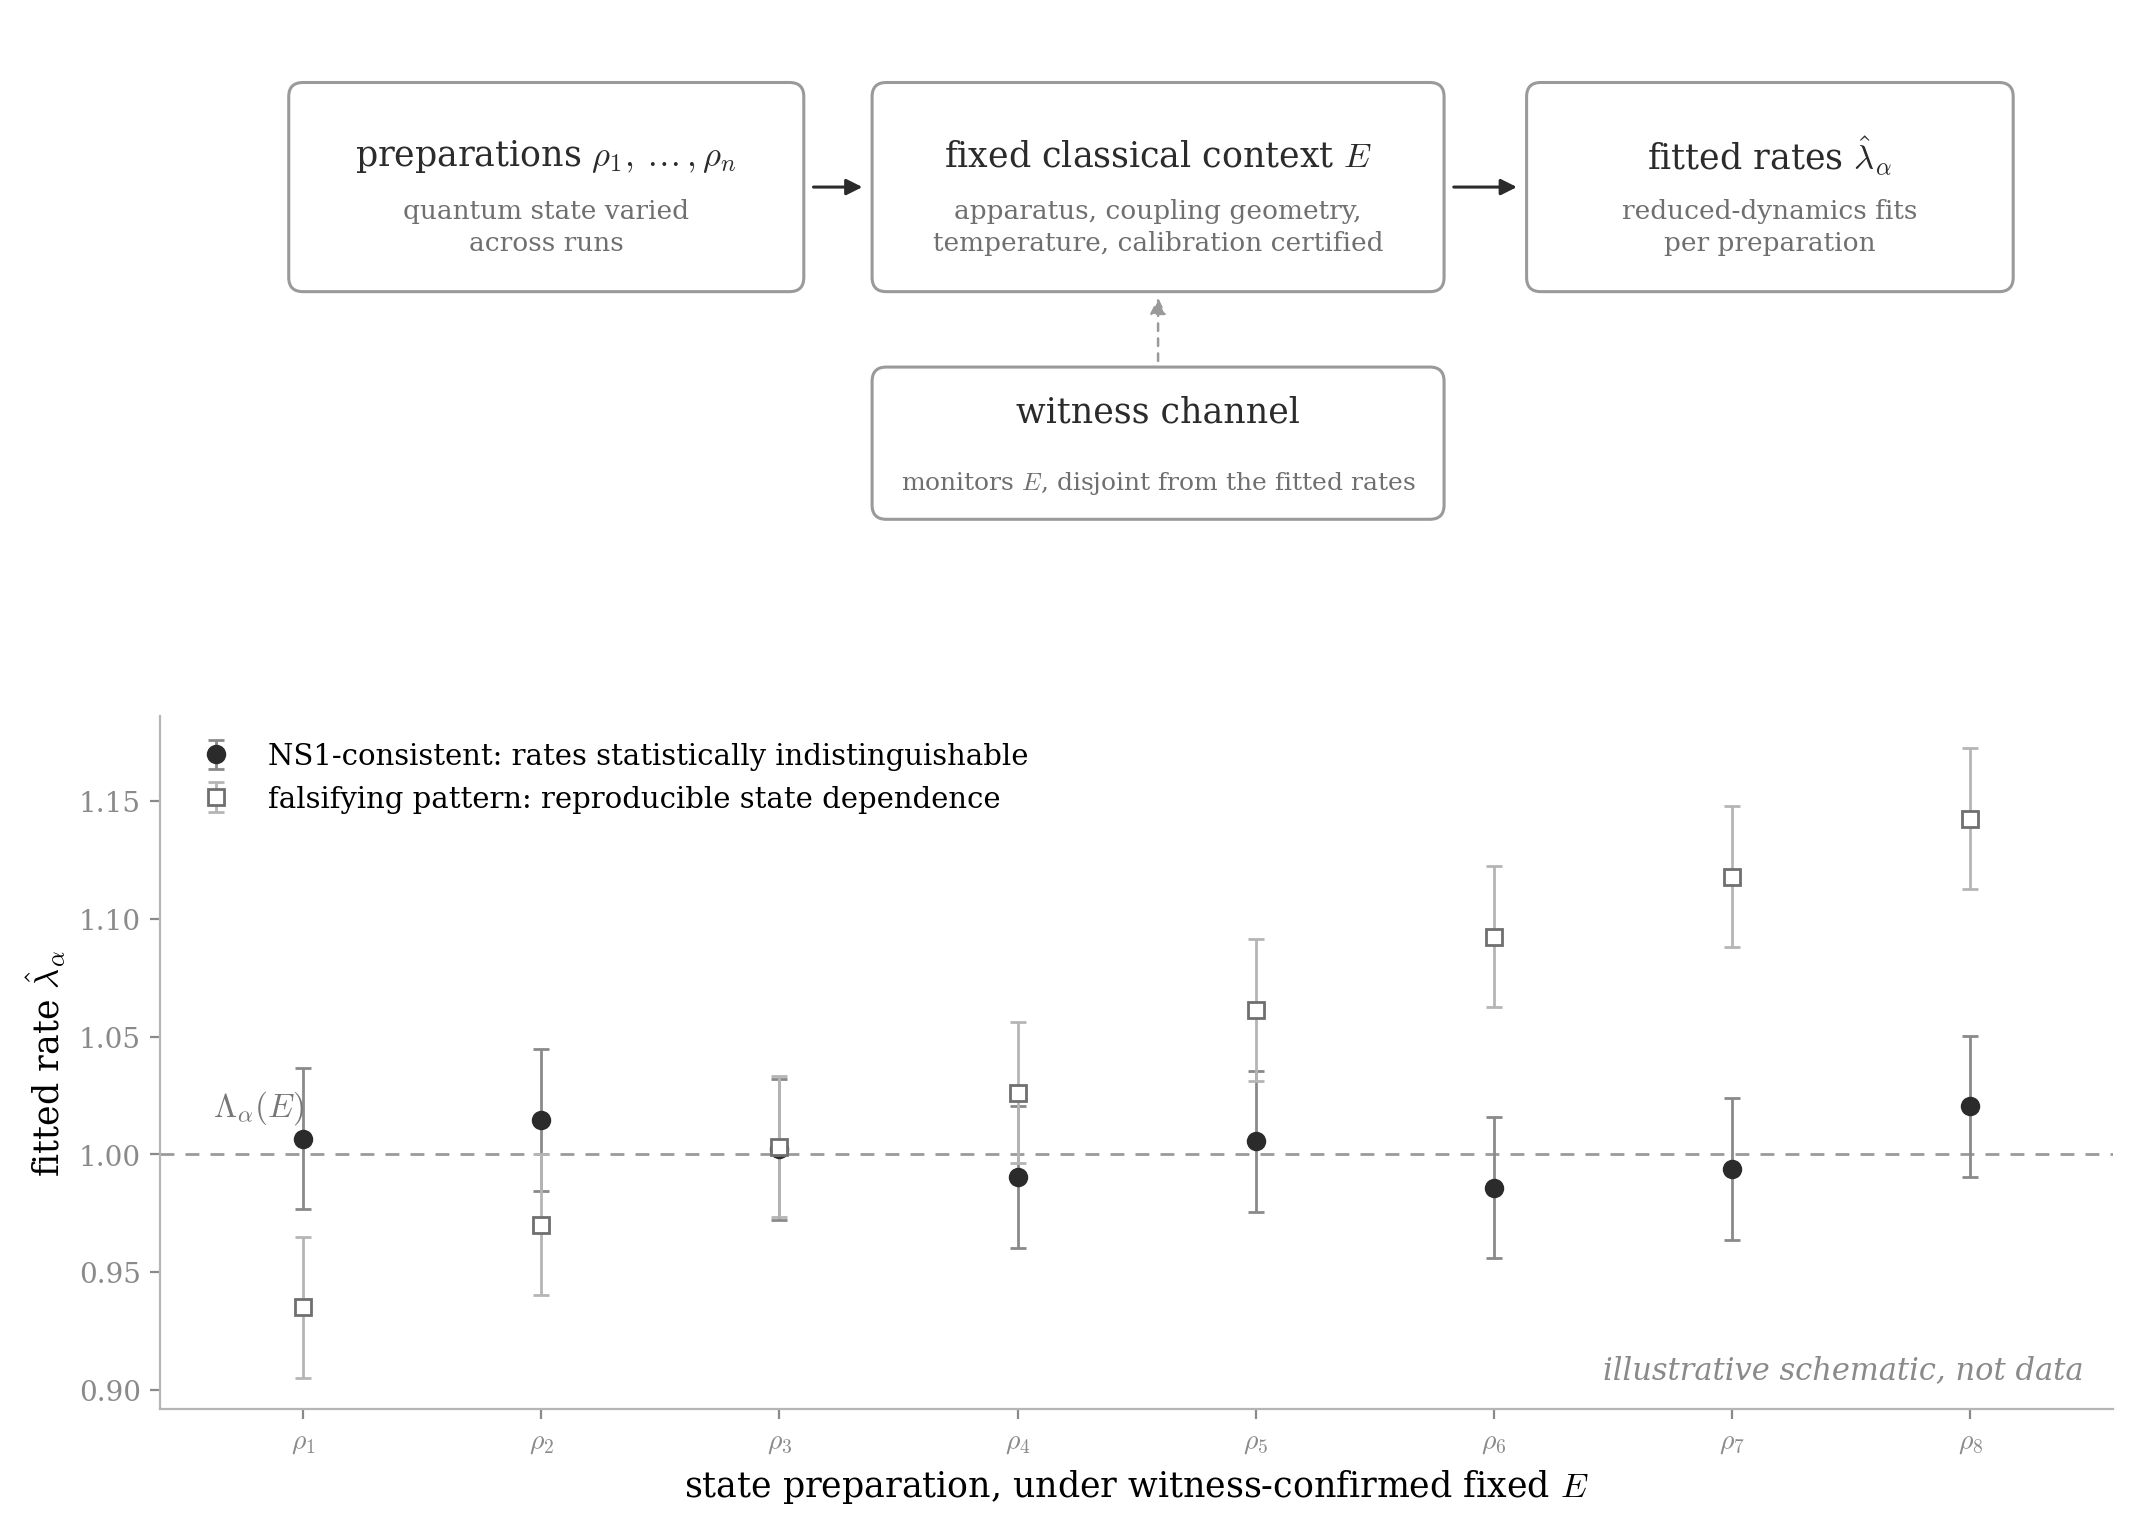
\includegraphics[width=0.95\linewidth]{fig_ns1_protocol_schematic.png}
\captionsetup{justification=raggedright,singlelinecheck=false}
\caption{\textbf{The NS1 rate-independence test.} Top: protocol flow.
State preparations are varied while the classical context \(E\) is
held fixed within independently certified tolerances and monitored by a
witness channel disjoint from the fitted rates; reduced-dynamics rate
parameters \(\hat\lambda_\alpha\) are fitted per preparation.
Bottom: the two outcome patterns of
Eq.~\eqref{eq:resolution_scaling}. Filled points: the NS1-consistent
outcome, fitted rates statistically indistinguishable across
preparations about the context-fixed value \(\Lambda_\alpha(E)\).
Open points: a falsifying pattern, reproducible state dependence of the
fitted rates under witness-confirmed fixed \(E\). The lower panel is
an illustrative schematic of the discrimination logic; no data are
represented.}
\label{fig:ns1_protocol_schematic}
\end{figure}

\paragraph{Why this prediction is nontrivial.}

A natural objection is that ordinary Lindblad generators are already
state-independent. In a fixed Markovian model,
\[
\mathcal L(\rho)
=
-i[H,\rho]
+
\sum_k \gamma_k
\left(
L_k\rho L_k^\dagger
-\frac12\{L_k^\dagger L_k,\rho\}
\right),
\]
the operators \(L_k\) and rates \(\gamma_k\) are model parameters, not
functions of \(\rho\).

The distinction is architectural. Standard open-system theory permits
many effective descriptions, including phenomenological fits,
preparation-dependent process reconstructions, memory-kernel models,
or descriptions affected by initial system--environment correlations.
Such descriptions may display preparation dependence without implying
superluminal signalling. SSAF imposes a stronger rule: within one
fixed context \(E\), no admissible map family, generator family, or
rate parameter may be selected as a function of the prepared state or
its outcomes.

The test is therefore not whether one can write a state-independent
Lindblad model. One can. The test is whether fixed-\(E\) data require
irreducible state-indexed generator selection to predict the observed
rates.

\paragraph{Operational criterion for fixed \(E\).}

The prediction requires that \(E\) be held operationally fixed across
preparations. \(E\)-stability is accepted only when the following are
satisfied simultaneously:

\begin{enumerate}[label=(\roman*), leftmargin=2.2em]
\item apparatus parameters, field strengths, coupling geometry,
temperature, pulse shapes, boundary conditions, and timing controls
remain within independently characterized drift tolerances;
\item the readout observable \(\mathcal O(E)\) is unchanged;
\item the environmental coupling profile is monitored by an
independent witness channel, such as a calibration qubit, interleaved
reference measurement, or auxiliary diagnostic whose observables are
not the fitted \(\lambda_\alpha\);
\item the criterion for declaring \(E\)-stability is fixed before the
rate fit is performed.
\end{enumerate}

A preparation that changes the preparation apparatus, environmental
state, coupling correlations, or readout interface constitutes a change
from \(E\) to \(E'\). The NS1 test applies only to runs retained by the
pre-declared independent witness criterion.

\paragraph{Initial correlations and context boundaries.}

Initial system--environment correlations can make reduced dynamics
preparation-dependent, and effective master-equation descriptions may
then display time-dependent or negative rates. SSAF treats the
preparation protocol, environmental state, coupling geometry, and
initial correlation structure as part of \(E\). If varying the
preparation changes those correlations, then the experiment has changed
context:
\[
E\longmapsto E'.
\]

Such cross-context variation is permitted. NS1 constrains only
within-context dependence:
\[
\lambda_\alpha(E,\rho)
\quad\text{is forbidden under fixed }E,
\]
while
\[
\lambda_\alpha(E)\neq\lambda_\alpha(E')
\]
is allowed.

\paragraph{Falsifiability and the context boundary.}

Folding correlation structure into \(E\) creates an obvious danger:
one might try to protect the theory by declaring every inconvenient
rate variation to be a hidden context shift. That move is not allowed.

The fixed-\(E\) judgment must be made by the independent witness
channel before inspecting the state-dependence of the fitted rates.
If a run is classified as \(E'\) only because the fitted rates changed,
the test is circular and has no empirical content.

The falsification condition is therefore:

\begin{quote}
If the independent witness channel certifies fixed \(E\), and the rate
fit still shows reproducible preparation-dependent rate variation, SSAF
is falsified.
\end{quote}

This does not give unconditional falsifiability under arbitrarily poor
context control. The test is only as strong as the independence and
sensitivity of the \(E\)-witness. A witness blind to the relevant
degree of freedom can misclassify a context shift as fixed-\(E\)
state-dependence. SSAF therefore makes a bounded falsifiable claim:
the framework is testable to the degree that \(E\) can be pinned down
by observables disjoint from the rates under test.

\paragraph{The measured quantity.}

The measured quantities are reduced-dynamics rate parameters, such as
decoherence or relaxation coefficients in a fitted generator model.
Experimentally, one prepares a family of states
\[
\{\rho_i\}
\]
spanning different purity, phase, population, and off-diagonal
structure; evolves each under the same independently certified context;
and fits time-resolved population or coherence signals to extract
\[
\lambda_\alpha^{(i)}.
\]

NS1 predicts
\[
\lambda_\alpha^{(i)}
=
\Lambda_\alpha(E)
\]
within statistical uncertainty for all \(i\). A statistically
significant regression of \(\lambda_\alpha^{(i)}\) against
\(\rho_i\), \(\Coh_E(\rho_i)\), phase angle, purity, or any
state-derived diagnostic, under witness-confirmed fixed \(E\), is a
falsification.

\paragraph{Operational divergence regime: fixed-context state variation.}

A concrete distinction between SSAF and unrestricted phenomenological
generator fitting appears when the context is independently verified
fixed while the prepared state is systematically varied.

Consider qubit preparations
\begin{equation}
\rho_0(\theta)
=
\begin{pmatrix}
p & r e^{i\theta}\\
r e^{-i\theta} & 1-p
\end{pmatrix},
\qquad
0\leq r\leq\sqrt{p(1-p)},
\label{eq:ns1_qubit_family}
\end{equation}
prepared under a monitored context
\[
E=(T,\lambda,S(\omega),\ldots).
\]

Under SSAF, the admissible dephasing rate is fixed by the context:
\begin{equation}
\gamma_\theta=\gamma(E),
\qquad
\frac{\partial\gamma}{\partial\theta}
=
\frac{\partial\gamma}{\partial p}
=
\frac{\partial\gamma}{\partial r}
=
0.
\label{eq:ns1_state_independent_rates}
\end{equation}

The off-diagonal amplitude satisfies
\begin{equation}
|c_\theta(t)|
=
|c_\theta(0)|e^{-2\gamma(E)t},
\label{eq:ns1_fixed_context_decay}
\end{equation}
with a single fixed-\(E\) CPTP family accounting for the entire
preparation ensemble.

By contrast, an unrestricted phenomenological fit may introduce
\begin{equation}
\gamma=\gamma(E,\rho_0),
\label{eq:state_conditioned_generator_selection}
\end{equation}
allowing different fitted rates for different preparations under the
same nominal environment. SSAF excludes this as a fixed-context
admissible operation.

The operational distinction is not whether each individual trajectory
can be fitted by a CPTP map in isolation. It is whether one affine
fixed-\(E\) update family accounts for the whole convex preparation
domain without preparation-indexed generator selection.

\paragraph{Adaptive tuning test.}

A result consistent with NS1, namely indistinguishable fitted rates
across preparations under confirmed fixed \(E\), does not establish
SSAF over all alternatives. Standard fixed-generator open-system
quantum mechanics gives the same result.

The discriminating test is adaptive generator selection. Run the same
protocol in two analysis modes:

\begin{enumerate}[label=(\roman*), leftmargin=2.2em]
\item a fixed-generator model, where one \(E\)-indexed generator is
used across the whole preparation ensemble;
\item a preparation-indexed model, where the generator may vary as a
function of \(\rho_i\) or observed statistics.
\end{enumerate}

If the preparation-indexed model gives a reproducible,
cross-validated improvement in rate prediction over the fixed-generator
baseline, and if the independent witness certifies fixed \(E\), then
NS1 is violated and SSAF is falsified.

A mere in-sample improvement is not sufficient, because it may reflect
overfitting. The improvement must survive pre-registered validation,
model-complexity penalties, and independent \(E\)-stability checks.

If no such improvement is found, the result supports NS1 only in the
limited sense that it constrains fixed-context state-conditioned
generator selection in the tested regime.

\paragraph{Discriminating regime.}

In a clean Markovian regime where the generator is already well
characterized, NS1 coincides with standard open-system expectations:
rates are state-independent by construction.

The prediction becomes most discriminating in boundary regimes where
experimenters observe apparent preparation-dependent effective decay
and must decide whether it reflects:

\begin{enumerate}[label=(\roman*), leftmargin=2.2em]
\item uncontrolled drift in \(E\), such as apparatus instability, SPAM
errors, environmental fluctuation, or calibration drift;
\item initial system--environment correlations that constitute a
change of context \(E\to E'\);
\item genuine state-dependent rate structure under confirmed fixed
\(E\).
\end{enumerate}

SSAF forbids option (iii). Once (i) and (ii) have been independently
controlled for, reproducible preparation-dependent rate variation under
fixed \(E\) falsifies the framework.

\begin{theorem}[Fixed-context affine consistency]
\label{thm:fixed_context_affine_consistency}
Let \(\mathcal D\subseteq\mathcal D(\mathcal H)\) be a convex
preparation domain under fixed context \(E\). Suppose a reduced
evolution rule is represented by
\[
F_E(\rho):=\Lambda_\rho^E(\rho),
\]
where each \(\Lambda_\rho^E\) is CPTP, but the selected map may depend
on \(\rho\).

If \(F_E\) is to represent a single fixed-context admissible evolution
law on \(\mathcal D\), then \(F_E\) must be affine:
\begin{equation}
F_E(p\rho_1+(1-p)\rho_2)
=
pF_E(\rho_1)+(1-p)F_E(\rho_2)
\label{eq:fixed_context_affine_requirement}
\end{equation}
for all \(\rho_1,\rho_2\in\mathcal D\) and \(p\in[0,1]\).

A preparation-indexed family
\[
\rho\mapsto\Lambda_\rho^E
\]
is therefore admissible under fixed \(E\) only if its induced map
\(F_E\) is the restriction of a single affine CPTP map on the convex
domain. Generic nonconstant preparation-indexed generator selection
violates this condition.
\end{theorem}

\begin{proof}
A fixed-context reduced evolution law must respect convex mixtures of
preparations. Preparing
\[
p\rho_1+(1-p)\rho_2
\]
as a classical mixture of procedures preparing \(\rho_1\) and
\(\rho_2\) cannot yield different reduced dynamics from preparing the
same density operator directly, unless the evolution depends on the
ensemble decomposition. Such dependence would make the map
decomposition-dependent and therefore not a well-defined affine
evolution on density operators.

Thus any fixed-context admissible evolution must satisfy
Eq.~\eqref{eq:fixed_context_affine_requirement}. A preparation-indexed
selection rule may accidentally satisfy this equality on a finite test
set, but unless the induced rule \(F_E\) extends to one affine CPTP map
on the convex domain, it cannot represent a single fixed-\(E\)
admissible law.

Generic nonconstant preparation-indexed generator selection fails this
affine condition because the map applied to a convex mixture is not the
convex mixture of the maps applied to its components.
\end{proof}

\paragraph{Experimental domains.}

Natural platforms include superconducting qubit arrays, trapped-ion
systems, and other controllable open quantum systems where classical
environmental parameters can be independently characterized while
state preparation is varied across a wide range of purity, phase, and
coherence values.

\paragraph{Failure modes.}

SSAF is structurally falsified if any of the following is required under
witness-confirmed fixed \(E\):

\begin{enumerate}[label=(\roman*), leftmargin=2.2em]
\item reduced-dynamics rates depend irreducibly on \(\rho\), its
ensemble decomposition, or state-derived diagnostics;
\item outcome-conditioned admissibility modification is required;
\item reproducing observed statistics demands nonlinear updates,
signalling, or non-CPTP reduced dynamics;
\item no single affine fixed-\(E\) CPTP family can account for the
convex preparation domain.
\end{enumerate}

\paragraph{Operational corollary: the context integrity sentinel.}

NS1 admits a direct engineering inversion. The rate-independence test
of this section holds \(E\) fixed and asks whether fitted rates move;
a sentinel trusts the fitted rates and asks whether \(E\) moved. Let a
probe system with any convenient preparation \(\rho_{\mathrm{probe}}\)
evolve under the certified context, let \(\hat\lambda_\alpha\) denote
continuously refitted reduced-dynamics rate parameters, and let
\(\Lambda_\alpha(E)\) be the certified baseline. Define the drift
statistic
\begin{equation}
\Delta_\alpha
:=
\hat\lambda_\alpha-\Lambda_\alpha(E).
\label{eq:sentinel_drift_statistic}
\end{equation}
Under Eq.~\eqref{eq:resolution_scaling}, \(\Delta_\alpha\) is
insensitive to the probe preparation, so any statistically significant
\(\Delta_\alpha\), at the power set by the fit variance, certifies
that the operational context has left its declared tolerance class,
\(E\to E'\), with no admissible attribution to the probe state. The
probe may therefore be the cheapest available preparation, and distinct
rate parameters \(\lambda_\alpha\) act as independent coordinates of
the context: a bank of continuously fitted rates is a partial
tomography of \(E\) rather than of any state. The sentinel is the
witness channel of the protocol above, placed in continuous engineering
use.

\paragraph{Scope of the corollary.}

The guarantee of attribution, that rate drift certifies context drift
rather than state dependence, is exactly the content of NS1 and holds
only within SSAF's admissible class. In any framework permitting
state-conditioned generator selection, a sentinel remains a useful
heuristic, but its alarms admit a second explanation; the guarantee is
what SSAF adds. Detection is limited by the certified baseline, the fit
variance, and the declared tolerance window, and the sentinel reports
that \(E\) changed, not which descriptor of \(E\) changed, unless
multiple rate coordinates are monitored and separately calibrated. No
new primitives, dynamics, or control channels are introduced: the
sentinel is a reading of Eq.~\eqref{eq:resolution_scaling}, not an
extension of it.


\section{Substrate, Scope, and Open Questions}
\label{sec:substrate_scope_open}

The framework as developed here is internally consistent and explicit
about what it derives. It is equally important to be explicit about what
it adopts and what it leaves open. The following statements bound the
claims of this paper and are not weaknesses to be read past; they are
the honest perimeter of the construction.

\paragraph{The adopted substrate.}

SSAF is constructed on the configuration space
\[
\Phi := \mathcal{D}(\mathcal{H}),
\]
the density operators on a Hilbert space, with the trace pairing
\[
\mathrm{Tr}(M\rho)
\]
serving as the interface expression through which addressable
distinctions are read
(Eq.~\ref{eq:addressability_relation}).

The Hilbert-space and operator geometry of \(\mathcal H\) is therefore
\emph{adopted} structure, not structure the framework generates.
Several features that might otherwise look like consequences of the
axioms enter with this substrate: the Born-weight assignment
(Appendix~A), the composite domain
\[
\mathcal{H}_A\otimes\mathcal{H}_B
\]
used in bipartite bookkeeping
(Eq.~\ref{eq:joint_envelope_def_core}), and any bound on jointly
admissible correlations inherited from standard quantum structure.

What SSAF contributes is the organization and dependency discipline
imposed \emph{on} this substrate: context-indexed admissibility,
compatibility, addressability, structural organization, sequencing, and
the NS1 constraint on what may depend on the state. It does not derive
the Hilbert-space substrate itself.

Deriving the Hilbert-space substrate from operational primitives that do
not already presuppose it is a separate reconstruction program
\cite{Hardy2001,Chiribella2010,MasanesMuller2011}, and is explicitly
\emph{not} attempted here.

\paragraph{Declared structural predicates and primitives.}

There is a structural asymmetry among the core objects. The
addressability relation \(\sim_E\) is \emph{constructed}: it is defined
through the trace pairing as equality of \(\mathrm{Tr}(M\rho)\) across
the interface \(\mathcal O(E)\)
(Eq.~\ref{eq:addressability_relation}).

By contrast, the compatibility predicate \(\Compat_E\), connectivity
structure \(\Gamma_E\), neighbourhood assignment \(\mathcal N_E\), and
admissibility measure \(\mu_E\) are \emph{declared} context-indexed
structural objects. They are constrained by the framework, separated by
role, and protected by NS1 from state-dependent retuning, but they are
not derived here from deeper operational primitives.

This is intentional. \(\Compat_E\) is not asked to secretly define
connectivity, neighbourhoods, topology, measure, or geometry; those
roles have been separated into \(\Gamma_E\), \(\mathcal N_E\), and
\(\mu_E\). The cost of that separation is that the structural layer is
explicitly specified rather than derived.

A future refinement may ground some or all of these objects in a more
basic overlap, distinguishability, or operational-access relation under
\(E\). For example, \(\Compat_E\) may be recoverable as the threshold
shadow of a graded compatibility or overlap functional, with
\(\Gamma_E\), \(\mathcal N_E\), and \(\mu_E\) recoverable from the same
graded structure. This paper does not establish such a derivation in
general. A finite-dimensional instance, recovering the declared
compatibility and connectivity of the charge-sector model as threshold
shadows of a single access functional, is worked in
Toy~\ref{toy:threshold_shadow_grounding}; the general question is
recorded with the open problems below.

\paragraph{Open questions.}

The following are not derivable from the SSAF primitives as they stand,
and the paper does not claim them.

\begin{enumerate}[label=(\roman*), leftmargin=2.2em]

\item \emph{Composition.}
The bipartite domain is taken as
\[
\mathcal{H}_A\otimes\mathcal{H}_B.
\]
Why composite description takes the tensor-product form, rather than
this being assumed, is not addressed.

\item \emph{The Born pairing.}
The weight assignment
\[
\mathrm{Tr}(M\rho)
\]
is adopted. Appendix~A shows it is the unique assignment consistent
with linearity in \(\rho\), convexity, and interface-only dependence,
but linearity in \(\rho\) is itself inherited from the substrate rather
than generated by SSAF.

\item \emph{The correlation bound.}
NS1 and admissibility together do not pin the set of jointly admissible
correlations to the quantum set. Structures satisfying no-signalling can
exceed the quantum, or Tsirelson, bound, so the bound requires geometric
content beyond dependency discipline alone. In the present framework,
that content enters through the adopted Hilbert-space/operator
substrate. See also the open problem in
Sec.~\ref{subsec:hyp_recursive_stratification}.

\item \emph{A state-independent context.}
The dependency discipline is meaningful only if the context \(E\) is
fixed independently of the configurations it governs. As specified here,
\(E\) indexes admissibility, compatibility, structural objects, and
updating data, but it is described by that role rather than constructed
from a prior physical background. A constructive, state-independent
specification of \(E\) would secure NS1 at its root; supplying one is
open.

\item \emph{Grounding the structural layer.}
The objects
\[
\Compat_E,
\qquad
\Gamma_E,
\qquad
\mathcal N_E,
\qquad
\mu_E
\]
are declared context-indexed structures. The paper separates their
roles and constrains their allowed dependencies, but does not derive
them from a single underlying principle. This question is now partially
resolved: Toy~\ref{toy:threshold_shadow_grounding} recovers
\(\Compat_E\) and \(\Gamma_E\), in the charge-sector
instantiation, as threshold shadows of a graded functional built from
\(E\)-accessible operations, with \(\mathcal N_E\) admitting a
natural candidate from the same object. The recovery of \(\mu_E\),
the uniqueness of the grounding, and the general case remain open;
absent a deeper operational reconstruction, such a grounding
would itself still depend on the adopted Hilbert-space/operator
substrate. Whether these objects can instead be grounded in primitives
strictly weaker than inner-product geometry is the point at which a
genuinely sub-substrate version of SSAF would have to begin.

\item \emph{Canonical spin structure.}
The spin proxy constructions show consistency of circulation-like
witnesses, closure constraints, and discrete labels with SSAF. They do
not derive \(SU(2)\), half-integer spectra, or spin-statistics from
SSAF primitives alone. Recovering those structures remains an open
problem.

\end{enumerate}

None of these is claimed as solved. They are recorded here because a
framework is more trustworthy for marking its own floor than for
concealing it.

\clearpage

\section{Appendix}
\label{sec:appendix}

\subsection{Long-Term Evolution of Extreme Coherence Basins}
\label{subsec:basin_evolution}

Over sufficiently extended realized orderings, gradual changes in
classical context \(E\) may alter the depth, margin extent, and
stability of extreme coherence basins. Such changes are represented as
boundary reconfiguration of admissibility, compatibility, connectivity,
neighbourhood, or measure structure under context re-indexing, not as
interior dynamics or state-dependent rate processes.

Slow admissibility re-expansion may permit basin shallowing without
singular behavior; observable consequences would manifest as changes in
boundary-localized ordering signatures. Whether extreme coherence
basins asymptotically approach null-admissibility limits, persist
indefinitely, or dissolve through cumulative boundary effects remains an
open structural question.

No mechanism, rate law, or timescale is asserted
\cite{Lindblad1976,Gorini1976,BreuerPetruccione2002,Watrous2018}.

\section*{Acknowledgments}

Mathematical formalization, including the drafting of definitions,
propositions, and proofs from the author's conceptual specifications
through iterative dialogue, together with manuscript structural
auditing, dependency analysis, LaTeX engineering, and the
implementation of the executable verification suite, was carried out
with substantial assistance from Anthropic's Claude. Some figures were
drafted with additional AI tools. The framework, its concepts and
axioms, the direction of all formal development, all physical claims,
and final responsibility for the content are the author's.

\section*{Code Availability}

The finite constructions of Appendix~D are accompanied by an
executable verification suite in which each covered toy's pass
conditions are encoded as machine-checked assertions; the suite runs
end to end and fails loudly on any violated claim. The suite verifies
the finite constructions' stated pass conditions; it does not
substitute for, and should not be read as machine verification of, the
proofs of the general results. The code is openly
available and permanently archived at
\url{https://doi.org/10.5281/zenodo.20634526}.

\section{Appendix A: Ordering Parameters and Diagnostic Machinery}
\label{app:diagnostic_machinery}

\subsection{Born Weights and Interface Statistics}
\label{appA:admissibility_born}

In SSAF, the wavefunction or density-operator description encodes a
configuration
\[
\rho\in\Phi
\]
under fixed \(E\), together with an interface determining which
distinctions are addressable. Resolution is restriction of
addressability within a realized ordering under fixed \(E\). When
reduced updating is represented, it uses linear CPTP maps indexed only
by \(E\), in accordance with NS1
\cite{Kraus1983,Lindblad1976,Gorini1976,Watrous2018,Gisin1989,
Gisin1990,Polchinski1991}.

For a fixed interface
\[
\mathcal O(E)
\]
and a POVM
\[
\{M_k(E)\}_k\subseteq\mathcal O(E),
\]
Born weights are given by
\[
p_k(E\mid\rho)
=
\mathrm{Tr}(M_k(E)\rho).
\]

These are interface-statistical weights associated with addressable
outcomes or records. They are not the structural admissibility measure
\[
\mu_E.
\]
The structural measure \(\mu_E\) assigns weight to admissible regions
inside \(\mathcal A(E)\); Born weights assign interface probabilities
for a given configuration and measurement vocabulary.

SSAF does not introduce a probabilistic selection rule, sampling
postulate, or dynamics-derived frequency theorem beyond standard
quantum theory. Decoherence analyses connect record stability and
interference suppression to \(|\psi|^2\)-consistent statistics in
ordinary laboratory environments
\cite{Zurek2003,Zurek2005,Schlosshauer2007,Joos2003}.

SSAF reads this as an empirically stable regularity of typical context
and interface choices, not as a new derivation of the Born rule. The
framework supplies a structural interpretation of why Born-consistent
statistics remain robust under common resolution regimes while keeping
the dependency discipline explicit.

Neither Born weights nor \(\mu_E\) may be used to select update maps,
generators, resolution rates, admissibility predicates, compatibility
relations, connectivity structures, neighbourhood assignments, or
sequencing rules as a function of \(\rho\), outcomes, ensemble
decompositions, or state-derived diagnostics.

\subsection{Born Weights as Interface Measures on Resolution Classes}
\label{subsec:born_rule_SSAF}

Born weights are representational interface measures on
\(E\)-specified resolution classes for a configuration \(\rho\). They
do not tune, bias, steer, or select outcomes. They also do not
parameterize admissible update families, generators, resolution rates,
admissibility predicates, compatibility predicates, connectivity
relations, neighbourhood assignments, admissibility measures, or
sequencing rules.

NS1 constrains update-family parameters to be indexed only by fixed
classical context \(E\), forbidding state- or outcome-conditioned
parameterization.

Fix \(E\) with outcome vocabulary
\[
\{\mathcal{R}_k(E)\}_k,
\]
a partition of the event space under \(E\). Introduce a positive
normalized representational measure
\[
\mu_{E,\rho}
\]
on the \(\sigma\)-algebra generated by these resolution classes, and
define
\begin{equation}
p_k
:=
\mu_{E,\rho}\bigl(\mathcal{R}_k(E)\bigr),
\qquad
p_k\geq 0,
\qquad
\sum_k p_k=1.
\label{eq:born_weight_measure_def}
\end{equation}

The measure \(\mu_{E,\rho}\) is representational: it assigns weights to
\(E\)-specified outcome or resolution classes for the given
configuration \(\rho\). It is not the structural admissibility measure
\(\mu_E\). The structural measure \(\mu_E\) assigns weight to admissible
regions inside \(\mathcal A(E)\); \(\mu_{E,\rho}\) assigns
interface-statistical weights to outcome classes for a fixed
configuration and interface.

\(\mu_{E,\rho}\) is not a rate law, dynamical mechanism, hidden
selection rule, sampling postulate, or CPTP update-family parameter.

In standard quantum mechanics, for a projective measurement,
\begin{equation}
p_k
=
\mathrm{Tr}\bigl(\rho\,\Pi_k(E)\bigr),
\label{eq:born_projective}
\end{equation}
or, more generally, for a POVM,
\begin{equation}
p_k
=
\mathrm{Tr}\bigl(\rho\,E_k(E)\bigr)
\label{eq:born_povm}
\end{equation}
\cite{Born1926,NielsenChuang2010,Watrous2018}.

Taking
\[
\mu_{E,\rho}\bigl(\mathcal{R}_k(E)\bigr)
:=
\mathrm{Tr}\bigl(\rho\,E_k(E)\bigr)
\]
recovers the usual POVM-induced probability measure in event-set form.

SSAF adopts the POVM-induced measure as the representational weight
assignment on \(E\)-specified resolution classes. This adoption is
justified by uniqueness: given linearity of expectations in \(\rho\),
convexity of \(\mathcal{D}(\mathcal{H})\), positivity, normalization,
and the requirement that weights are determined solely by
\(\mathcal{O}(E)\) and \(\rho\) without additional hidden structure, the
POVM-induced measure is the unique assignment satisfying these
constraints~\cite{Gleason1957,BuschLahtiMittelstaedt2003}.

Resolution behavior, rates, thresholds, channel strengths, and
generator coefficients remain governed exclusively by fixed \(E\). They
cannot depend on \(\rho\), anticipated outcomes, ensemble
decompositions, or state-derived diagnostics, in accordance with NS1 and
linear CPTP representability~\cite{Lindblad1976,Gorini1976,Gisin1989,
Gisin1990,Polchinski1991}.

\paragraph{Separation from admissibility measure.}

The notation distinguishes two different measures:
\[
\mu_E
\qquad
\text{and}
\qquad
\mu_{E,\rho}.
\]

The structural admissibility measure
\[
\mu_E:
\mathcal P(\mathcal A(E))
\to
[0,\infty]
\]
weights admissible regions and is context-indexed only.

The Born/interface measure
\[
\mu_{E,\rho}
\]
weights outcome or resolution classes for a specified configuration
\(\rho\) and interface.

Neither measure may select update maps, generators, resolution rates,
admissibility predicates, compatibility predicates, connectivity
relations, neighbourhood assignments, or sequencing rules as a function
of outcomes, ensemble decompositions, or state-derived diagnostics.

\paragraph{Theory-change triggers.}

The framework requires revision if any of the following are established:

\begin{enumerate}[label=(\roman*), leftmargin=2.2em]

\item state-dependent update-family parameterization,
\[
\lambda_\alpha=\lambda_\alpha(E,\rho);
\]

\item experimentally accessible retro-addressability within a fixed
realized ordering under fixed \(E\);

\item controllable signalling via outcome-conditioned map selection or
state-conditioned retuning;

\item state-conditioned retuning of \(\Gamma_E\), reassignment of
\(\mathcal N_E\), or reweighting of \(\mu_E\) under fixed \(E\);

\item necessity of non-CPTP reduced dynamics to preserve positivity or
normalization.

\end{enumerate}

Born weights quantify \(E\)-specified resolution-class weights for
\(\rho\). They do not supply outcome control, do not modify admissible
updating, and do not alter NS1 parameter dependence.

\subsection{Morphological Records as Diagnostics}
\label{appA:morphological_records_diagnostics}

Observable structure in matter is treated as a diagnostic record of
realized ordering under admissibility restriction, not as evidence of
new fundamental dynamics.

Under sustained coupling, environment-driven restriction may suppress
phase-incompatible continuations while allowing persistence of
admissible ordering patterns. The resulting morphology is a coarse
diagnostic of which ordering descriptions remained stable under the
declared context \(E\), without implying steerability, agency, hidden
optimization, or a new generator.

Records constrain the space of admissible reconstructions; they do not
determine a unique mechanism. Persistent patterns across ordinary
physics encode long-wavelength, integrated ordering structure rather
than pointwise transport histories~\cite{Bagnold1941,Hooke2005,
BinneyTremaine2008,LinShu1964}.

Morphological records do not determine admissibility, compatibility,
connectivity, neighbourhood structure, admissibility measure, update
maps, generator parameters, or resolution rates. They may motivate a
model-specific reconstruction, but they do not retune the fixed
\(E\)-indexed structural layer.

\subsection{Pinching-Based Coherence Witness and Covariant Monotonicity}
\label{app:pinching_coherence_witness}

Let the fixed context \(E\) determine a reference block structure
\[
\{\Pi_m(E)\}_m
\]
with
\[
\Pi_m(E)\Pi_n(E)=\delta_{mn}\Pi_m(E),
\qquad
\sum_m\Pi_m(E)=I.
\]

Define the pinching channel
\begin{equation}
\Delta_E(\rho)
:=
\sum_m
\Pi_m(E)\rho\Pi_m(E),
\label{eq:app_pinching_channel}
\end{equation}
which is CPTP and depends only on
\(E\)~\cite{Kraus1983,Watrous2018}.

Define the diagnostic
\begin{equation}
V_E(\rho)
:=
D\!\bigl(\rho\,\|\,\Delta_E(\rho)\bigr)
=
\mathrm{Tr}\bigl[
\rho(\log\rho-\log\Delta_E(\rho))
\bigr]
\geq 0.
\label{eq:app_V_relative_entropy_record}
\end{equation}

The quantity \(V_E(\rho)\) vanishes iff \(\rho\) is block-diagonal in
the \(E\)-reference structure. It is a coherence witness relative to
the declared context, not a primitive, not a resource postulate, and not
a dynamical driver~\cite{Baumgratz2014,ChitambarGour2019}.

In particular, \(V_E\) does not determine admissibility,
compatibility, connectivity, neighbourhood structure, admissibility
measure, sequencing, update-family selection, generator coefficients,
or resolution rates.

If the adopted \(E\)-indexed update family satisfies
\(\Delta_E\)-covariance,
\begin{equation}
\Delta_E\circ\mathcal{T}^E_\Delta
=
\mathcal{T}^E_\Delta\circ\Delta_E,
\label{eq:app_dephasing_covariance}
\end{equation}
then \(V_E\) is non-increasing:
\begin{equation}
V_E\bigl(\mathcal{T}^E_\Delta(\rho)\bigr)
\leq
V_E(\rho)
\qquad
\forall\,\Delta\geq 0.
\label{eq:app_V_contractivity}
\end{equation}

\begin{proof}
By data processing of quantum relative entropy under CPTP
maps~\cite{Petz1986,Wilde2017,NielsenChuang2010},
\begin{equation}
D\!\bigl(
\mathcal{T}^E_\Delta(\rho)
\,\|\,
\mathcal{T}^E_\Delta(\Delta_E(\rho))
\bigr)
\leq
D\!\bigl(
\rho
\,\|\,
\Delta_E(\rho)
\bigr).
\label{eq:app_DPI_step}
\end{equation}

By \(\Delta_E\)-covariance,
\[
\mathcal{T}^E_\Delta(\Delta_E(\rho))
=
\Delta_E(\mathcal{T}^E_\Delta(\rho)).
\]
Therefore the left-hand side of
Eq.~\eqref{eq:app_DPI_step} is
\[
V_E\bigl(\mathcal{T}^E_\Delta(\rho)\bigr),
\]
and the desired inequality follows.
\end{proof}

\begin{remark}[Diagnostic status]
The monotonicity in Eq.~\eqref{eq:app_V_contractivity} is conditional
on the chosen update family being \(\Delta_E\)-covariant. It is not a
general law of SSAF and does not define admissible updating. The result
shows that, under a standard covariance condition, a context-indexed
coherence witness behaves monotonically under the represented update.
It remains diagnostic and cannot be used as a state-dependent steering
or retuning parameter under NS1.
\end{remark}

\subsection{A Monotone Ordering Parameter for Admissibility Reduction}
\label{app:ordering_parameter}

This subsection constructs an illustrative monotone scalar bookkeeping
label for realized admissible ordering chains under fixed \(E\). It
does not define time, generate ordering, modify admissibility, or alter
the axioms~\cite{Watrous2018,Wilde2017,NielsenChuang2010}.

Fix \(E\) with pointer decomposition
\[
\{\Pi_i(E)\}_i
\]
and pinching map
\[
\Delta_E(\rho)
=
\sum_i \Pi_i(E)\rho\Pi_i(E).
\]

Define the coherence diagnostic
\begin{equation}
\mathrm{Coh}_E(\rho)
:=
S(\Delta_E(\rho))-S(\rho),
\label{eq:relative_entropy_coherence_pointer}
\end{equation}
where \(S(\cdot)\) is von Neumann entropy.

This quantity is diagnostic only. It does not parameterize ordering,
admissibility, compatibility, connectivity, neighbourhood structure,
admissibility measure, update-family selection, generators, or
resolution rates~\cite{Baumgratz2014,ChitambarGour2019}.

Restrict to chains
\[
\rho_0\prec_E\rho_1\prec_E\rho_2\prec_E\cdots
\]
along which
\[
\mathrm{Coh}_E(\rho_{k+1})
\leq
\mathrm{Coh}_E(\rho_k).
\]

A sufficient condition for such monotonicity is
\(\Delta_E\)-covariance of the adopted fixed-\(E\) maps, as in
Sec.~\ref{app:pinching_coherence_witness}
\cite{Petz1986,Baumgratz2014,ChitambarGour2019,Wilde2017}.

Define the cumulative ordering-depth diagnostic
\begin{equation}
\Theta(\rho_n)
:=
\sum_{k=0}^{n-1}
\bigl(
\mathrm{Coh}_E(\rho_k)
-
\mathrm{Coh}_E(\rho_{k+1})
\bigr).
\label{eq:theta_def}
\end{equation}

Under monotonicity, each summand is nonnegative. The sum telescopes:
\begin{equation}
\Theta(\rho_n)
=
\mathrm{Coh}_E(\rho_0)
-
\mathrm{Coh}_E(\rho_n)
\geq 0.
\label{eq:theta_telescope}
\end{equation}

Thus \(\Theta\) is a chain-relative bookkeeping label. It is not an
ordering-independent state function, not a resource, and not a
generator of sequencing.

In deep coherence-basin descriptions, \(\Theta\) may increase slowly as
\(\mathrm{Coh}_E(\rho_n)\) approaches its attainable floor under fixed
\(E\). This is not a claim about halted ordering or frozen dynamics. It
only records how an \(E\)-defined diagnostic varies along an admissible
chain.

When mapped to observer-level reconstructions, such saturation may
correspond to a domain-of-definition failure for nontrivial clock
reconstruction: if the interface yields no variance-bearing markers, no
nontrivial
\[
t=\mathcal R(\tau;E)
\]
is licensed
(Sec.~\ref{subsec:cd_clock_domain_limits}).

\subsection{Optional Basin-Depth and Gradient Diagnostics}
\label{app:basin_depth_gradients}

When restricting to pure configurations, the Fubini--Study gradient
\[
\nabla_{\mathrm{FS}}\mathrm{Coh}_E
\]
when differentiable, is a diagnostic sensitivity descriptor in the
chosen chart. It is not a dynamical vector field, force law, flow, or
gradient-descent rule~\cite{BengtssonZyczkowski2006,Nakahara2003}.

Fix a declared basin sector
\[
\mathcal B\subseteq\mathcal A(E),
\]
a core subset
\[
\mathcal B_{\mathrm{core}}\subseteq\mathcal B,
\]
and a boundary neighbourhood
\[
\partial_E\mathcal B\subseteq\mathcal B.
\]

The objects \(\mathcal B\), \(\mathcal B_{\mathrm{core}}\), and
\(\partial_E\mathcal B\) are representational and must be stated
explicitly. In particular, \(\partial_E\mathcal B\) is not assumed to be
a topological boundary, metric boundary, connected-component boundary,
or \(\mathcal N_E\)-boundary unless a model-specific construction
declares it.

A basin-depth proxy is
\begin{equation}
\Delta_{\mathcal B}\mathrm{Coh}_E
:=
\Bigl[
\inf_{\rho\in\mathcal B_{\mathrm{core}}}
\mathrm{Coh}_E(\rho)
-
\sup_{\rho\in\partial_E\mathcal B}
\mathrm{Coh}_E(\rho)
\Bigr]_+.
\label{eq:app_basin_depth}
\end{equation}

This is a chart- and boundary-convention-dependent contrast statistic.
It introduces no update rule, no basin dynamics, no force law, no
optimization principle, and no state-conditioned retuning.

The sign convention in Eq.~\eqref{eq:app_basin_depth} should be read as
part of the chosen diagnostic convention. If a model treats larger
\(\mathrm{Coh}_E\) as deeper rather than shallower, the corresponding
contrast may be reversed. No physical claim depends on this convention
unless a model explicitly assigns an interpretation to the sign.

Neither
\[
\Theta,
\qquad
\nabla_{\mathrm{FS}}\mathrm{Coh}_E,
\qquad
\Delta_{\mathcal B}\mathrm{Coh}_E
\]
may be used to select update maps, generators, resolution rates,
admissibility predicates, compatibility predicates, connectivity
relations, neighbourhood assignments, admissibility measures, or
sequencing rules as a function of \(\rho\), outcomes, ensemble
decompositions, or state-derived diagnostics.

\subsection{Coherence Measures}
\label{app:coherence_measures}

The coherence functional
\[
\mathrm{Coh}_E:\Phi\to\mathbb{R}_{\geq 0}
\]
is a diagnostic assigning a scalar indicator of off-diagonal structure
relative to an \(E\)-specified reference decomposition. It is
descriptive only. It does not act as an operator, enter admissibility
criteria, define compatibility, determine connectivity, assign
neighbourhoods, reweight admissible regions, or parameterize update
families~\cite{Baumgratz2014,ChitambarGour2019}.

Fix pointer projectors
\[
\{\Pi_i(E)\}_i
\]
with
\[
\Pi_i(E)\Pi_j(E)=\delta_{ij}\Pi_i(E),
\qquad
\sum_i\Pi_i(E)=I,
\]
and pinching map
\[
\Delta_E(\rho)
:=
\sum_i\Pi_i(E)\rho\Pi_i(E).
\]

A coherence diagnostic may be required to satisfy:

\begin{enumerate}[label=(C\arabic*), leftmargin=2.5em]

\item \textbf{Faithfulness:}
\[
\mathrm{Coh}_E(\rho)=0
\quad\Longleftrightarrow\quad
\Delta_E(\rho)=\rho.
\]

\item \textbf{Nonnegativity:}
\[
\mathrm{Coh}_E(\rho)\geq 0
\]
for all \(\rho\in\Phi\).

\item \textbf{Convexity:}
\[
\mathrm{Coh}_E\!\left(\sum_j p_j\rho_j\right)
\leq
\sum_j p_j\mathrm{Coh}_E(\rho_j).
\]

\item \textbf{Monotonicity on a declared class:}
for \(\Delta_E\)-covariant maps \(\mathcal{T}^E\) satisfying
\[
\Delta_E\circ\mathcal{T}^E
=
\mathcal{T}^E\circ\Delta_E,
\]
one has
\begin{equation}
\mathrm{Coh}_E(\mathcal{T}^E(\rho))
\leq
\mathrm{Coh}_E(\rho).
\label{eq:coh_monotone_class}
\end{equation}

\end{enumerate}

A standard choice satisfying these requirements is the relative-entropy
coherence
\begin{equation}
\mathrm{Coh}_{E,\mathrm{rel}}(\rho)
:=
S(\Delta_E(\rho))-S(\rho)
=
D\!\left(\rho\,\|\,\Delta_E(\rho)\right)
\geq 0,
\label{eq:relative_entropy_coherence}
\end{equation}
with monotonicity following from data processing plus
\(\Delta_E\)-covariance~\cite{Petz1986,Baumgratz2014,ChitambarGour2019,Wilde2017}.

The functional \(\mathrm{Coh}_E\) never appears in admissibility
criteria, compatibility predicates, connectivity relations,
neighbourhood assignments, admissibility measures, resolution
operators, generator coefficients, update-family parameterization, or
sequencing rules~\cite{Gisin1989,Gisin1990,Polchinski1991,Watrous2018}.

\subsection{Bounds and Inequalities}
\label{subsec:coherence_bounds}

For finite dimension
\[
d=\dim\mathcal{H}<\infty,
\]
the relative-entropy coherence satisfies
\begin{equation}
0
\leq
\mathrm{Coh}_{E,\mathrm{rel}}(\rho)
\leq
\log d,
\label{eq:coh_rel_bounds}
\end{equation}
with the upper bound attained by maximally coherent pure states relative
to the declared \(E\)-reference structure~\cite{Baumgratz2014,ChitambarGour2019}.

For \(\Delta_E\)-covariant \(\mathcal{T}^E\),
\begin{equation}
\mathrm{Coh}_{E,\mathrm{rel}}(\mathcal{T}^E(\rho))
\leq
\mathrm{Coh}_{E,\mathrm{rel}}(\rho).
\label{eq:coh_rel_monotone}
\end{equation}

For bipartite \(AB\) with local dephasings
\[
\Delta_{E,A}\otimes\Delta_{E,B},
\]
the relative-entropy coherence is additive on product states:
\begin{equation}
\mathrm{Coh}_{E,\mathrm{rel}}(\rho_A\otimes\rho_B)
=
\mathrm{Coh}_{E,\mathrm{rel}}(\rho_A)
+
\mathrm{Coh}_{E,\mathrm{rel}}(\rho_B).
\label{eq:coh_rel_additive_products}
\end{equation}

For correlated \(\rho_{AB}\), one has the diagnostic bound
\begin{equation}
\mathrm{Coh}_{E,\mathrm{rel}}(\rho_{AB})
\leq
\mathrm{Coh}_{E,\mathrm{rel}}(\rho_A)
+
\mathrm{Coh}_{E,\mathrm{rel}}(\rho_B)
+
I(A{:}B)_\rho,
\label{eq:coh_rel_correlation_bound}
\end{equation}
where
\[
I(A{:}B)_\rho
=
S(\rho_A)+S(\rho_B)-S(\rho_{AB})
\]
is the quantum mutual information~\cite{NielsenChuang2010,ChitambarGour2019}.

All bounds in this subsection are diagnostic only. They do not modify
admissibility, compatibility, connectivity, neighbourhood structure,
admissibility measure, sequencing, or map/generator parameters. All
admissible parameter dependence remains indexed only by fixed \(E\).

\subsection{Illustrative Examples}
\label{appA:illustrative_examples}

\paragraph{Incoherent state.}

If
\[
\Delta_E(\rho)=\rho,
\]
then
\[
\mathrm{Coh}_E(\rho)=0.
\]

\paragraph{Single-qubit coherent pure state.}

Let
\[
|\psi\rangle
=
\alpha|0\rangle+\beta|1\rangle,
\qquad
|\alpha|^2+|\beta|^2=1.
\]
For
\[
\rho=|\psi\rangle\langle\psi|,
\]
one has
\[
S(\rho)=0
\]
and
\[
\Delta_E(\rho)
=
\mathrm{diag}(|\alpha|^2,|\beta|^2).
\]
Thus
\[
\mathrm{Coh}_{E,\mathrm{rel}}(\rho)
=
H(|\alpha|^2,|\beta|^2),
\]
which is positive unless
\[
|\alpha|=0
\quad\text{or}\quad
|\beta|=0.
\]

\subsection{Illustrative Entanglement Diagnostics}
\label{appA:entanglement_diagnostics}

A separable state has the form
\[
\rho_{AB}
=
\sum_i p_i\,
\rho_A^{(i)}\otimes\rho_B^{(i)}.
\]
Such states belong to the separable hull
\[
\mathrm{Sep}_E(A{:}B)
\]
when the component marginals are admissible under the declared
context-indexed marginal domains.

A non-separable
\[
\rho_{AB}\notin\mathrm{Sep}_E(A{:}B)
\]
is a witness of non-factorizable joint admissibility when
\[
\rho_{AB}\in\mathcal A_{AB}(E).
\]

This is a structural constraint on the joint admissible sector, not a
signalling channel and not an update rule. Entanglement diagnostics do
not modify admissibility, affect rates, retune structural primitives, or
extend addressability beyond what is licensed by the fixed-\(E\)
interface, envelope constraints, and realized ordering.

\section{Appendix B: Dictionary-Level Mappings}
\label{appB:dictionary_mappings}

This appendix is a translation layer providing dictionary-level mappings
from spacetime-first, thermodynamic, and condensed-matter language into
SSAF primitives:
\[
\Phi=\mathcal D(\mathcal H),
\qquad
\mathcal A(E),
\qquad
\mathrm{Compat}_E,
\qquad
\sim_E,
\qquad
\Gamma_E,
\qquad
\mathcal N_E,
\qquad
\mu_E.
\]

No new primitives, dynamics, or predictions are introduced. Each mapping
is admissible only if it can be stated as a change of description
applied to fixed admissibility, compatibility, addressability, and
declared structural organization under fixed \(E\). All update-family
parameterization remains indexed only by \(E\), in accordance with NS1.

\subsection{Structural Primitives: Admissibility, Addressability, and Organization}
\label{appB:admissibility_addressability_primitive}

Apparent structure in spacetime descriptions maps to three SSAF layers:

\begin{enumerate}[label=(\roman*), leftmargin=2.2em]

\item \emph{Admissibility:}
which configurations are admitted under \(E\), expressed by
\[
\mathcal A(E)\subseteq\Phi.
\]

\item \emph{Addressability:}
which distinctions among admissible configurations are resolvable under
\[
\mathcal O(E),
\]
expressed through \(\sim_E\).

\item \emph{Structural organization:}
how admissible configurations are organized, related, and weighted under
fixed \(E\), expressed through
\[
\Gamma_E,
\qquad
\mathcal N_E,
\qquad
\mu_E.
\]

\end{enumerate}

Any phrase such as ``persists,'' ``emerges,'' or ``is selected'' is
shorthand for a constraint-closure statement under fixed \(E\), together
with an addressability statement about which distinctions survive under
the interface. Where needed, the structural layer may further specify
connectivity, neighbourhood structure, or admissibility measure.

Multiple admissible continuation classes may be depicted as a
``branching'' diagram for intuition. Termination corresponds to
constraint non-closure, and pruning corresponds to loss of
addressability. Any such depiction must be convertible back into an
\(E\)-indexed claim about
\[
\mathcal A(E),
\qquad
\sim_E,
\qquad
\mathrm{Compat}_E,
\qquad
\Gamma_E,
\qquad
\mathcal N_E,
\qquad
\mu_E,
\]
or into an explicitly declared subset of those structures.

\subsection{Reconstruction Dictionary: \(\Phi\)-Space to Spacetime}
\label{appB:reconstruction_dictionary}

Fix \(E\) and an observational interface \(\mathcal O(E)\). A
reconstruction
\begin{equation}
\mathcal M_E:
\mathcal A(E)/{\sim_E}
\longrightarrow
\mathsf{Desc}_{\mathrm{st}}(E)
\label{eq:phi_to_spacetime_map}
\end{equation}
compresses admissible and addressable structure into effective
spacetime descriptors.

Reconstructed spatial distance summarizes phase-local accessibility or
derived neighbourhood relations under the interface. Reconstructed
clock time summarizes correlation-based assignment of an operational
parameter to an already-realized acyclic sequencing relation
\cite{PageWootters1983,Rovelli1991}. Reconstructed curvature or
geometry summarizes constraint nesting, connectivity organization,
neighbourhood variation, admissibility concentration, and
domain-dependent variation in sequencing granularity.

This mapping does not posit a hidden spacetime substrate and does not
derive, replace, or modify general relativity~\cite{Einstein1915,Wald1984}.
It is a dictionary for translating effective spacetime descriptions into
SSAF-compatible structural language.

Apparent paradoxes in descriptions of the wavefunction are often
category errors: treating a configuration-space object as a material field, a
spacetime-local substance, or a subjective probability report. In SSAF,
nonlocal correlations, interference, and entanglement are represented as
features of shared admissible and joint-admissible structure, not as
superluminal influence.

\subsection{Program Alignment: Decoherence and Envariance}
\label{appB:zurek}

SSAF is structurally aligned with the decoherence program
\cite{Zurek2003}. Decoherence explains interference suppression through
system-environment entanglement, yielding dynamically stable pointer
descriptions~\cite{Zurek2003,Schlosshauer2007}.

Within SSAF, this is mapped to context-indexed restriction of
addressability and admissible structure. Coherence-basin language may
be used for sectors in \(\Phi\) whose declared constraint and
neighbourhood structure remains well-posed under fixed \(E\), but basin
language remains representational unless a model explicitly supplies
topology, metric structure, or basin dynamics.

Zurek's envariance constrains Born weights via symmetry under
environment-assisted transformations without subjective probability or
state-dependent reduction~\cite{Zurek2005,Zurek2009}. SSAF is
compatible with these constraints and adds no alternative statistical
postulate.

The departure from standard decoherence lies not in statistical
structure but in the semantic treatment of outcome persistence:
decoherence and envariance constrain robustness and weights, while SSAF
tracks irreversible restriction of addressability within a realized
ordering. Admissible updating remains linear CPTP throughout.

\subsection{Dictionary Entries}
\label{appB:dictionary_entries}

\subsubsection{Entropy}
\label{appB:entropy_mapping}

``Entropy'' maps to an interface-dependent diagnostic of accessible
distinctions under fixed \(E\). Informally, it tracks how many
configurations or records remain distinguishable and
sequencing-addressable within
\[
\mathcal A(E)/{\sim_E}.
\]

Entropy increase maps to expansion of accessible volume under
coarse-graining, loss of fine addressability, or irreversible coupling
\cite{Prigogine1977,Carroll2010}. Von Neumann entropy is an interface
diagnostic for accessibility and uncertainty in the represented quantum
description; it is not a dynamical driver~\cite{vonNeumann1955,NielsenChuang2010}.

Entropy should not be identified with the structural admissibility
measure \(\mu_E\) unless a model-specific construction explicitly
defines such an identification. Likewise, entropy is distinct from Born
weights \(\mu_{E,\rho}\), which assign interface-statistical weights to
outcome classes for a given configuration.

Apparent information loss maps to non-addressability: fine distinctions
remain in \(\Phi\) while becoming inaccessible under \(\mathcal O(E)\),
in line with decoherence's separation of global unitary description
from effective classical records~\cite{Zurek2003,Zurek2005}.

\subsubsection{Thrustless Motion}
\label{appB:thrustless_motion_mapping}

Reports of ``thrustless'' or ``inertia-defying'' motion map to cases
where a classical kinematic narrative is applied outside its licensed
reconstruction domain. The dictionary entry prevents category errors
while remaining compatible with linear CPTP updating and
decoherence-based record stability~\cite{Lindblad1976,Gorini1976,Zurek2003}.

No reactionless-drive mechanism, momentum-violation claim, force law, or
state-conditioned admissibility retuning is introduced. Such reports, if
modeled at all, require an explicit reconstruction map from admissible
and addressable structure into an effective spacetime description.

\subsubsection{Topological/Anyonic Transport}
\label{appB:map_topological_anyon_transport}

Fix \(E\) with admissible region
\[
\mathcal A(E)\subseteq\Phi
\]
and a compatibility-supported sector
\[
\mathcal K\subseteq\mathcal A(E).
\]

An ``anyonic'' transport channel is classified, at dictionary level, as
an envelope-level restriction within \(\mathcal K\) limiting
addressability to configurations supporting model-declared
non-contractible circulation witnesses.

This entry is representational. It does not assert that
\(\mathcal K\) is automatically a connected component of \(\Gamma_E\),
a neighbourhood under \(\mathcal N_E\), a topological region, or a
measured region under \(\mu_E\). Any such identification requires a
model-specific construction.

Magnetic order and superconducting transport correspond to distinct
phase roles within a declared compatibility-supported sector:
envelope-local sectorization rather than competing primitive order
parameters. Effective two-dimensionality is a structural constraint on
envelope stability. Nontrivial phase winding is sustained when
admissible envelopes admit declared non-contractible circulation
witnesses not erased by further admissibility restriction.

No retro-admissibility, outcome steering, state-dependent resolution
rates, non-CPTP updating, or primitive topology is introduced.

\subsubsection{Momentum Duality (Abraham--Minkowski)}
\label{appB:momentum_duality_mapping}

``Momentum'' in field-matter contexts maps to effective
ordering-transport bookkeeping whose numerical form depends on the
partition convention across coherence supports.

The Abraham form emphasizes ordering transport distributed across field
modes; the Minkowski form emphasizes transport bound to
medium-supported organization. The invariant content is total
accounting relative to a specified context and explicit partition
convention~\cite{Abraham1909,Minkowski1908,Barnett2010}.

No new momentum law is introduced. The dictionary mapping does not alter
admissibility, compatibility, connectivity, neighbourhood structure,
admissibility measure, update-family selection, or NS1 dependency
discipline.

\subsection{Thermodynamic Correspondences}
\label{appB:thermodynamic_correspondences}

Thermodynamic quantities in this appendix are dictionary-level
reconstructions. They summarize accessible structure under a specified
context and operational partition. They are not SSAF primitives and do
not modify admissibility, compatibility, addressability, connectivity,
neighbourhood structure, admissibility measure, sequencing, CPTP
updating, or NS1.

Let \(S\) denote an effective entropy functional summarizing accessible
admissible configuration volume under fixed context. This \(S\) is an
interface-level thermodynamic reconstruction. It should not be
identified with the structural admissibility measure \(\mu_E\) unless a
model-specific construction explicitly supplies that identification.

Fix auxiliary descriptors
\[
(\eta,\kappa)
\]
and an energetic constraint coordinate
\[
\mathcal{E}_{\mathrm{th}}.
\]
The temperature correspondence is
\begin{equation}
\frac{1}{T}
\equiv
\alpha
\left(
\frac{\partial S}{\partial \mathcal{E}_{\mathrm{th}}}
\right)_{\eta,\kappa},
\label{eq:temperature_correspondence}
\end{equation}
where \(\alpha\) is a units-setting constant~\cite{Callen1985,Reif1965}.

Higher effective temperature corresponds, in this dictionary, to smaller
reconstructed inverse-temperature slope; lower effective temperature
corresponds to larger slope or stiff accessibility response, depending
on the chosen thermodynamic convention. The invariant content is the
gradient relation itself, not a new SSAF dynamical law.

Equilibration corresponds to absence of a net accessibility gradient
between interacting reconstructed domains.

\paragraph{Four thermodynamic laws.}

\begin{itemize}[leftmargin=*]

\item \textbf{Zeroth law: equilibrium.}
Equilibrium corresponds to equality of reconstructed inverse
temperature:
\[
\left(
\frac{\partial S}{\partial \mathcal{E}_{\mathrm{th}}}
\right)^{(A)}_{\eta,\kappa}
=
\left(
\frac{\partial S}{\partial \mathcal{E}_{\mathrm{th}}}
\right)^{(B)}_{\eta,\kappa}.
\]

\item \textbf{First law: energetic bookkeeping.}
Work corresponds to externally specified changes in constraint
descriptors. Heat corresponds to accessibility changes under fixed
external controls. This is bookkeeping over a declared operational
partition, not a new conservation postulate inside SSAF.

\item \textbf{Second law: irreversibility.}
The reconstructed thermodynamic statement
\[
\Delta S_{\mathrm{total}}\geq 0
\]
maps to environment-driven loss of fine addressability and the formation
of record-stable descriptions under irreversible coupling, compatible
with decoherence-based accounts~\cite{Zurek2003,BreuerPetruccione2002};
within the framework, the failure of admissible linear recovery is
Proposition~\ref{prop:no_cptp_recovery}.
It does not assert destruction of configurations in \(\Phi\).

\item \textbf{Third law: vanishing accessibility response.}
In the low-temperature limit, accessible reconstructed variation becomes
stiff: the effective entropy change available under further energetic
constraint variation approaches a limiting behavior fixed by the chosen
thermodynamic model~\cite{Callen1985}. In conventional thermodynamic
language this is expressed by the approach to a limiting entropy and
vanishing accessibility to additional states as \(T\to 0\).

\end{itemize}

These correspondences introduce no new dynamics and preserve CPTP
updating and NS1 throughout.

\subsubsection{Non-Equilibrium Bookkeeping}
\label{app:neq_first_law_bookkeeping}

Let \(\Omega\) be a modeled region with reconstruction-indexed context
\[
E_\tau.
\]
The operational bookkeeping identity is
\begin{equation}
\frac{d}{d\tau}
U_\Omega(E_\tau)
=
\dot{Q}_\Omega(E_\tau)
-
\dot{W}_\Omega(E_\tau)
+
\dot{\mathcal{F}}_\Omega(E_\tau),
\label{eq:neq_first_law_flux_term}
\end{equation}
where \(\dot{\mathcal{F}}_\Omega\) summarizes non-equilibrium transport
and storage contributions, such as advective flux, boundary injection,
or gradient storage, that must be made explicit when \(E_\tau\) encodes
sustained structure or exchange.

This is an accounting identity, not a new conservation law, dynamical
equation, generator, or update rule. The channels
\[
\dot{Q}_\Omega,
\qquad
\dot{W}_\Omega,
\qquad
\dot{\mathcal{F}}_\Omega
\]
are context-indexed descriptors determined by \(E_\tau\) and the stated
operational partition. They are not outcome-conditioned controls and
may not be selected as functions of \(\rho\), outcomes, ensemble
decompositions, or state-derived diagnostics.

The non-equilibrium bookkeeping layer does not retune
\[
\Gamma_E,
\qquad
\mathcal N_E,
\qquad
\mu_E,
\]
and does not alter NS1-consistent CPTP updating.

\subsection{Extreme-Regime Vocabulary}
\label{appB:extreme_regime_vocabulary}

\subsubsection{Extreme Ordering and Addressability}
\label{appB:extreme_ordering_accessibility}

In extreme regimes, admissibility restriction may be severe while the
operational interface remains coarse. Many admissible configurations may
be observationally indistinguishable under fixed \(E\): a realized
sequencing record can remain structurally well-defined while
cross-addressability collapses into large equivalence classes under
\(\sim_E\).

This is \emph{non-cross-addressability}: admissible structure may remain
defined while many internal distinctions are no longer jointly
addressable through the interface.

When a clock reconstruction
\[
t=\mathcal R(\tau;E)
\]
is introduced, extreme regimes are those in which addressable
restriction markers become sparse or unavailable in the reconstructed
parameterization. Where reconstruction markers are not available,
\(t\) is undefined and the articulation density
\[
\delta(\tau):=\frac{dN}{d\tau}
\]
is undefined, not small.

As an illustrative mapping, an extreme coherence basin may be regarded
as an effective interface across which internal distinctions are not
cross-addressable under \(\mathcal O(E)\), even when a stable external
signature remains addressable. This introduces no mechanism, no
interior reconstruction claim, and no additional dynamics.

\subsubsection{Coherence-Freeze}
\label{appB:coherence_freeze}

In sufficiently deep coherence basins, addressable sequencing markers
may become increasingly sparse under fixed \(E\). Under a spacetime-based
reconstruction, this may be described as asymptotic ``freezing'' of
effective progression, without requiring cessation of admissible CPTP
updating.

The SSAF claim is strictly structural: addressability can collapse while
admissibility remains consistent, acyclic, and NS1-compatible.
``Freezing'' refers to failure of time-extended kinematic narration
under extreme non-cross-addressability, not to dynamical arrest.

\subsubsection{Information Persistence vs.\ Accessibility}
\label{appB:info_persistence}

Configurations excluded from further addressable refinement remain
elements of \(\Phi\) even when no additional cross-addressable refinement
is available under \(\mathcal O(E)\). This is the
admissibility/addressability distinction, not a hidden-variable claim.

SSAF does not assert that \(\sim_E\)-equivalence classes can be inverted
to recover an interior state, nor does it introduce dual boundary
encodings.

``Information persistence'' is shorthand for \(\Phi\)-level
configuration existence. Any quantitative information statistic is an
interface-level diagnostic computed from \(\mathcal O(E)\) and does not
parameterize admissibility, compatibility, connectivity, neighbourhood
structure, admissibility measure, sequencing, or NS1-licensed update
data.

\subsubsection{Kinematic Limits}
\label{appB:kinematic_limits}

Classical narratives of infall, deformation, or transport are licensed
only when the reconstruction protocol yields a stable mapping from
ordering relations to a time-parameterized description.

In extreme regimes, non-cross-addressability renders such narratives
ill-defined even though admissible CPTP updating remains well-posed.
Stable external signatures may still register at boundary-level
addressability under \(\mathcal O(E)\); this is not a claim about
interior processes.

All ``suppression'' language denotes a domain-of-definition limit:
\[
t=\mathcal R(\tau;E)
\]
is undefined when ordering markers are not addressable, and articulation
density is likewise undefined.

\subsubsection{Boundary-Dominated Admissibility Filtering}
\label{appB:boundary_dominated_filtering}

Deformation-based metaphors, such as ``spaghettification,'' are optional
interpretive vocabulary. The structural content is that under
sufficiently restrictive admissibility, compatibility or constraint
relations may be resolved predominantly at the boundary of a declared
admissible domain without licensing time-extended deformation narratives
for internal configurations.

No deformation mechanism, stress law, internal evolution, metric
singularity, or alteration of known physics is introduced.

A boundary in this vocabulary is a domain-of-definition boundary for a
declared reconstruction. It is not automatically a topological boundary,
metric surface, connected-component boundary of \(\Gamma_E\), boundary
of \(\mathcal N_E\), or measured boundary under \(\mu_E\), unless a
model-specific construction explicitly supplies that interpretation.

\subsubsection{Null-Addressability Basins}
\label{appB:null_addressability}

A \emph{null-addressability basin} is a limiting description in which
\(\sim_E\)-equivalence classes become so large that no internal
distinctions remain addressable by \(\mathcal O(E)\), and no sequencing
markers support time-extended narration.

This is not a dynamical singularity and does not signal CPTP failure.
Hierarchical descriptive layers may remain structurally defined in
\(\Phi\) while excluded from addressability.

In such limits, well-posed content is restricted to explicitly declared
fixed-\(E\) structure, including:

\begin{enumerate}[label=(\roman*), leftmargin=2.2em]

\item membership in
\[
\mathcal A(E);
\]

\item compatibility or envelope predicates on the admissible domain;

\item interface-level equivalence classes
\[
\Phi/{\sim_E};
\]

\item declared connectivity, neighbourhood, or measure structure,
\[
\Gamma_E,
\qquad
\mathcal N_E,
\qquad
\mu_E,
\]
where those objects remain meaningful under the limiting description.

\end{enumerate}

Claims requiring inversion of \(\sim_E\), interior reconstruction, or
time-extended kinematic narration are undefined.

\subsubsection{Null-Core, Boundary-Regenerative Structures}
\label{appB:null_core_boundary_regenerative}

When interior non-cross-addressability is extreme while boundary-level
addressability remains nontrivial, one may classify the regime as
\emph{null-core, boundary-regenerative}.

``Null-core'' is an observer-side fact: under fixed \(E\), interior
distinctions are not cross-addressable and do not support kinematic
narration.

Boundary-localized admissibility reconfiguration may make additional
boundary-level distinctions addressable under \(\mathcal O(E)\) for
limited reconstructed intervals. Under fixed \(E\), this is a
boundary-level reconstruction effect. If the admissible domain itself is
enlarged or the interface changes, the description is instead a
context re-indexing
\[
E\mapsto E'.
\]

This is not leakage, traversal, or information flow across an ontic
barrier.

Any use of ``flux'' denotes a coarse-grained accounting label for
change in boundary-level addressable summaries under a reconstruction
parameterization. It is not conserved current flow from an interior, not
transport across an ontic boundary, and not an additional dynamical
channel beyond linear CPTP updating.

Terms such as ``effective radiation,'' if used, are coarse-graining
labels for cumulative boundary-level addressability change admitting a
thermal-like summary. They do not derive Hawking or Unruh effects and
introduce no new channels~\cite{Hawking1975,Unruh1976}.

\subsubsection{No Bulk-Boundary Duality or Holographic Claims}
\label{appB:scope_holography_limit}

Nothing in the foregoing mappings asserts bulk-boundary duality,
holographic encoding, or interior reconstructability from boundary data.
SSAF introduces no encoding map, reconstruction prescription, or
information-recovery mechanism.

Boundary-localized diagnostics arise from admissibility, addressability,
and declared structural organization under environment-driven
restriction, not from a dual boundary theory~\cite{Susskind1995,
Maldacena1998}.

Appendix~B provides controlled vocabulary for extreme-regime
descriptions: deep basins as regimes of severe admissibility restriction
and non-cross-addressability under \(\mathcal O(E)\), possibly admitting
stable boundary diagnostics while rendering interior kinematic narration
ill-posed. These mappings do not modify the core framework.

\section{Appendix C: Thought Experiments}
\label{app:thought_experiments}

This appendix introduces no new postulates, operators, structural
primitives, or dynamical commitments. Each thought experiment is
non-operational and functions only as an interpretive stress test of
admissibility, envelope closure, addressability, and non-retroactive
sequencing under NS1.

\subsection{Thought Experiment: Ancestor-Elimination Without Retrocausation}
\label{appC:toy_ancestor_elimination}

This thought experiment checks whether SSAF generates logical paradoxes
from hypothetical ancestor-elimination narratives, such as the
``grandfather paradox'' family~\cite{Lewis1976}. It introduces no
admissible intervention protocol, no new dynamics, and no empirical
claim.

Its only purpose is to check consistency of admissibility, sequencing,
and addressability under a fixed context \(E\).

\subsubsection{Setup}

We work at the level of configuration space
\[
\Phi=\mathcal D(\mathcal H).
\]

Membership in \(\Phi\) does not imply realization, admissibility,
addressability, compatibility, connectivity, or operational
connectability. The ambient configuration space contains many abstract
configurations that are not jointly addressable within any given
realized description.

Let
\[
\mathcal E_\star\subseteq\mathcal A(E)
\]
denote the realized admissible envelope corresponding to the observer's
description under fixed \(E\). Sequencing is realized within
\(\mathcal E_\star\), with environment-driven admissibility restriction,
interface-limited addressability, and NS1-compatible updating.

The declared structural layer
\[
\Gamma_E,
\qquad
\mathcal N_E,
\qquad
\mu_E
\]
may describe organization, neighbourhoods, or admissible-region weight
inside the fixed-\(E\) domain, but none of these objects licenses
cross-envelope intervention or state-dependent retuning.

Assume there exists some configuration
\[
\rho_{\mathrm{alt}}\in\Phi
\]
whose internal relational pattern would be read in an external narrative
as ``ancestor elimination occurs.'' No assumption is made that
\(\rho_{\mathrm{alt}}\) is admissible under \(E\), addressable through
\(\mathcal O(E)\), compatible with \(\mathcal E_\star\), or connectable
from within the realized envelope.

\subsubsection{Question}

Does the abstract existence of \(\rho_{\mathrm{alt}}\) entail that an
identity instantiated within \(\mathcal E_\star\) can:

\begin{enumerate}[label=(\roman*), leftmargin=2.2em]
\item access \(\rho_{\mathrm{alt}}\);
\item reconfigure into \(\rho_{\mathrm{alt}}\);
\item induce a contradiction within the realized ordering of
\(\mathcal E_\star\)?
\end{enumerate}

\subsubsection{Structural Resolution}

The answer is negative in all three cases.

The reason is structural. SSAF introduces no admissible cross-envelope
operation. Under fixed \(E\), representational updating may be written
as a linear CPTP map on \(\Phi\), but any protocol-level claim is
defined only on its licensed domain. For the realized description here,
that domain is \(\mathcal E_\star\).

Thus an admissible in-domain update has the form
\begin{equation}
\mathcal T^E_\Delta:
\mathcal E_\star
\to
\mathcal E_\star,
\label{eq:ancestor_in_domain_update}
\end{equation}
or, more precisely, a CPTP map whose operationally licensed use is
restricted to the realized envelope.

No admissible rule is introduced whose domain or codomain spans
distinct incompatible envelopes. No rule licenses ``jumping'' from
\(\mathcal E_\star\) to \(\rho_{\mathrm{alt}}\).

Therefore \(\rho_{\mathrm{alt}}\) may exist abstractly in \(\Phi\) while
remaining non-admissible, non-addressable, or non-connectable from
within \(\mathcal E_\star\). The attempted intervention is not
``forbidden by a dynamical law.'' It is \emph{undefined} as an
admissible operation inside the fixed-\(E\) description.

This differs from closed timelike curve constructions, which add
cross-history or self-consistency constraints by design~\cite{Novikov1989,Deutsch1991}.

\subsubsection{Absence of Paradox}

No retrocausation occurs because no realized ordering inside
\(\mathcal E_\star\) is modified. No resequencing occurs because the
realized sequencing record remains fixed under \(E\). No contradiction
is generated because \(\rho_{\mathrm{alt}}\) is not an operand of the
admissible update, addressability, or sequencing rules defined on
\(\mathcal E_\star\).

Any paradox arises only if one assumes that abstract existence in
\(\Phi\) implies operational accessibility. SSAF does not license that
inference.

\subsubsection{Relation to Superposition: Interpretive Only}

As an interpretive analogy, the relevant distinction mirrors a familiar
pattern in quantum mechanics: multiple formal descriptions may be
written, while operational addressability and realized records remain
restricted by the interface and admissibility conditions actually in
force~\cite{Schrodinger1935}.

No additional mechanism is introduced here. The analogy does not imply
many-world branching, retrocausation, hidden variables, or physical
travel between configurations.

\paragraph{Constraint: no retro-addressability across envelopes.}

Configurations outside the realized envelope of a fixed-\(E\)
description are not operands of any admissible updating, sequencing, or
intervention within that description. Retrocausation, resequencing, and
cross-envelope addressability are structurally undefined in SSAF.

\subsection{Thought Experiment: Sequencing Through Compatibility Thresholds}
\label{appC:thought_sailor_sequencing}

This thought experiment gives an intuitive illustration of sequencing,
admissibility, compatibility, addressability, and environment-driven
restriction in SSAF. It is a conceptual aid only: it introduces no new
ontology, dynamics, operator, primitive, or physical mechanism.

\paragraph{Scope: metaphor only.}

The sailor, boat, sea, wind, and storms are allegorical devices. They
do not correspond to agents, forces, trajectories, control variables,
spacetime motion, or hidden steering.

They serve only to visualize:

\begin{enumerate}[label=(\roman*), leftmargin=2.2em]
\item compatibility or constraint restriction;
\item loss of addressability;
\item context re-indexing;
\item non-retroactive sequencing under NS1.
\end{enumerate}

Any use of ``moment,'' ``earlier,'' ``later,'' ``past,'' or ``future''
refers only to ordering-depth and observer-level clock reconstruction
conventions, not to a primitive time coordinate.

\subsubsection{Setup}

Consider an idealized sailor on a boat in which nothing is steered:
there is no choice, no targeting, no feedback, and no control. The
scene represents a coarse reconstruction of admissible structure in
\(\Phi\), not a literal trajectory through space.

Many configurations compatible with that coarse picture may exist as
elements of
\[
\Phi=\mathcal D(\mathcal H).
\]
The thought experiment concerns only which configurations remain
admissible, compatible, and addressable within a realized ordering
description.

The structural primitives invoked here are those already defined, and
none is retuned as a function of the state, outcomes, ensemble
decompositions, or diagnostic quantities
(Axiom~\hyperref[ax:NS1]{VII}).

\subsubsection{Compatibility Thresholds}

A \emph{compatibility threshold} is a boundary in the declared
constraint structure where certain continuations cease to be licensed
within the relevant admissible description.

Under fixed \(E\), such a threshold is represented as restriction within
the already declared admissibility and compatibility structure. If the
classical background itself changes, for example through altered
couplings, boundary conditions, apparatus settings, or noise structure,
then the correct representation is context re-indexing:
\[
E\mapsto E'.
\]

No transition is initiated by an agent. No outcome is targeted. No
state-conditioned rule is introduced.

Configurations that fail the relevant compatibility or closure
conditions do not disappear and are not retro-modified. They remain
elements of \(\Phi\), but they may become non-addressable relative to
the realized ordering and stated interface. Sequencing proceeds as
progressive restriction of what remains addressable within the realized
description, not as navigation, steering, or outcome targeting.

\subsubsection{Sequencing}

The within-description narrative corresponds to a single realized
ordering chain sustained under admissibility and addressability
restriction. The ordering is acyclic: distinctions excluded by a
registered restriction do not re-enter the same realized ordering under
the same fixed context
(Proposition~\ref{prop:registered_implies_terminal_nonaddr}).

In an observer-level reconstruction, this may be encoded as temporal
succession. At the level of \(\Phi\), no global time coordinate is
introduced. Time is a post-ordering encoding of sequencing under
constraint, not a primitive.

If the context changes from \(E\) to \(E'\), the resulting description
belongs to a re-indexed ordering domain. It is not a retroactive rewrite
of the original fixed-\(E\) ordering record.

\subsubsection{Phase Descriptors and Apparent Randomness: Interpretive Only}

In coarse descriptions, outcome-like variation can be represented as
sensitivity to fine compatibility or constraint structure in \(\Phi\)
relative to admissibility boundaries under a declared context.

Small, untracked differences in phase descriptors, initial
configuration, interface resolution, or coupling geometry may change
which continuations remain licensed across a threshold. This can yield
different realized ordering records without introducing choice,
state-dependent control, nonlinear updating, or outcome-conditioned
map selection.

This paragraph is interpretive. It introduces no stochastic selection
rule and no new SSAF dynamical claim.

\subsubsection{Absence of Paradox}

Configurations corresponding to ``storms that might have occurred'' or
``routes that might have been taken'' may remain elements of \(\Phi\),
but they are not automatically compatible, addressable, or jointly
licensed with the realized ordering under \(\mathcal O(E)\).

Abstract existence does not imply operational accessibility.

No paradox arises because nothing leaves the realized envelope and
nothing retro-modifies the realized ordering. There is no rerouting,
retrocausation, or cross-envelope travel. There is only
domain-local persistence under admissibility and addressability
restriction.

\subsubsection{Interpretive Conclusion}

This construction illustrates how the abundance of configurations in
\(\Phi\) is compatible with exclusive realized sequencing under a
declared context: many descriptions can be written, while realized
experience corresponds to an ordering record whose addressability may
narrow under NS1-safe restriction.

Apparent temporal flow is an observer-level projection of this ordering,
not a primitive. The sailor metaphor is useful only so long as it stays
in its lane: it visualizes restriction and addressability loss, not
motion, choice, control, or dynamics.

\subsection{Thought Experiment: A Sequencing Gate Without Shared
Destinations}
\label{appC:thought_experiment_sequencing_gate}

\paragraph{Scope (non-empirical).}
This thought experiment is a structural stress test. It does not assert
that any ``gate'' can be engineered, nor does it introduce any new
mechanism, postulate, or axiom. It asks only: \emph{if} a description
treats an apparatus as inducing an entry-envelope restriction for
realized sequencing under a fixed classical context, what does SSAF
require about addressability, shared access, and non-retroactive
sequencing?

\paragraph{Setup.}
Fix a classical context $E$ and admissible set
$\mathcal{A}(E) \subset \Phi$. In this thought experiment, an
apparatus $G$ is represented as restricting admissible participation
in a realized ordering to some entry envelope
$\mathcal{E}(E) \subseteq \mathcal{A}(E)$.

We assume only: (i) sequencing is non-retroactive within a realized
ordering; (ii) all restriction and updating depends only on the
classical context, never on the quantum state (NS1); (iii)
addressability is defined within a realized ordering via the fixed
interface $\mathcal{O}(E)$; and (iv) existence in $\Phi$ does not
imply operational accessibility from within a realized ordering.

\paragraph{Two entries (two contexts).}
A first group $\mathcal{G}_1$ enters under context $E_1$, yielding
entry envelope $\mathcal{E}(E_1)$ and realized sequencing chain
$\Sigma_1$. A second group $\mathcal{G}_2$ enters under a distinct
context $E_2 \neq E_1$ (a distinct activation, timing, or boundary
condition folded into $E$), yielding chain $\Sigma_2$.

The intuitive but structurally illicit expectation is that if $G$ is
``the same gate'' and entry conditions are ``similar enough,'' then
$\mathcal{G}_2$ should join the chain already realized by
$\mathcal{G}_1$.

\begin{lemma}[Overlap of entry envelopes does not imply shared ordering
access]
\label{lem:gate_overlap_no_shared_access}
Fix contexts $E_1$ and $E_2$. Even if the entry envelopes overlap,
\[
\mathcal{E}(E_1) \cap \mathcal{E}(E_2) \neq \varnothing,
\]
this does not license a statement that a later entry under $E_2$ can
join the realized ordering $\Sigma_1$ or gain addressability to
$\Sigma_1$-internal distinctions.
\end{lemma}

\begin{proof}
Overlap is a statement about structural membership in $\Phi$: there
exist configurations admissible as elements under both envelope
descriptions. However, the content of $\Sigma_1$ is a realized
ordering record whose addressability is defined relative to
$\mathcal{O}(E_1)$ \emph{within that ordering}. Joining $\Sigma_1$
from a later entry would require reopening addressable distinctions
already fixed by the realized restriction record of $\Sigma_1$,
violating non-retroactive sequencing
(Lemma~\ref{lem:gate_overlap_no_shared_access}). Alternatively, it would require
an outcome- or history-conditioned selection rule targeting a
previously realized chain, which is excluded by NS1. Structural
overlap of envelopes does not imply shared ordering access.
\qedhere
\end{proof}

\paragraph{Consequences.}
A distinct entry instance can at most:
\begin{enumerate}[label=(\roman*), leftmargin=2.2em]
\item \emph{Realize a distinct ordering.} $\mathcal{G}_2$ realizes
$\Sigma_2$, which may be structurally similar to $\Sigma_1$ but is
not addressably identical to it.
\item \emph{Null-entry under mismatch.} If $\mathcal{E}(E_2)$ admits
no admissible continuation under the prevailing description, no
realized sequencing chain is admitted. This is a domain-of-definition
failure, not a dynamical breakdown.
\end{enumerate}

\paragraph{``Same destination'' as a category error.}
In SSAF, ``destination'' language is a reconstruction-level
projection. An apparatus description can at most constrain which
ordering relations may be realized under a stated context via an entry
envelope. It cannot target a previously realized chain without
introducing forbidden outcome-conditioned steering or retroactive
selection of addressable configurations.

\paragraph{Interpretive Conclusion.}
The gate scenario isolates a central SSAF distinction: admissible
configuration structure may be plentiful in $\Phi$ while
addressability remains exclusive to a realized ordering record.
Repeatable structure does not entail repeatable access.

\paragraph{Bridge.}
We now turn to toy surrogates that illustrate these constraints at the
level of bookkeeping only.

\section{Appendix D: Axiom Unit Tests and Structural Clarifiers}
\label{toy:models}

This appendix collects small toy constructions used as axiom unit tests
and structural clarifiers for SSAF. An \emph{axiom unit test} is a
minimal concrete construction that checks whether a stated structural
property holds in a specific bookkeeping setting, analogous to a unit
test in software that checks one function at a time.

The toys here check that admissibility, sequencing, structural
organization, and addressability behave as claimed under fixed
classical context \(E\); that no forbidden state- or outcome-indexed
dependencies sneak in; and that domain-of-definition failures, such as
envelope non-closure rendering cross-configuration claims undefined,
arise exactly when the framework says they should.

No toy is offered as an empirical signature or prediction. Each
functions solely as a consistency witness for the semantics of the main
text. All constructions remain consistent with linear CPTP updating,
used representationally, and NS1, which requires state-independent
parameterization fixed only by \(E\)~\cite{Watrous2018,Wilde2017,
NielsenChuang2010}.

\subsection{Axiom Unit Test: Basin-Supported Circulation as a Spin Proxy}
\label{subsec:spin_closure_discreteness}

\subsubsection{What This Section Does and Does Not Claim}
\label{subsubsec:spin_quantization_admissibility}

The goal of this unit test is to show that spin-like discrete labels
can appear \emph{consistently} within SSAF without deriving them from
new dynamics. Specifically, if an effective reconstruction uses
discrete ``spin-like'' labels, their discreteness is licensed as a
closure and single-valuedness condition on a circulation witness used
for bookkeeping.

This discreteness is not a consequence of basin depth alone and is not
introduced as a new dynamical postulate.

\paragraph{What this section does not do.}

This section does not derive \(\mathrm{SU}(2)\), half-integer spin,
spin-statistics, or any microscopic generator. Those remain open
problems identified in the main text.

The purpose here is narrower: to show that discrete labels of the kind
spin requires are structurally admissible within the framework, arising
from well-posedness conditions on circulation witnesses supported by
declared admissible loop classes.

\paragraph{Closure admissibility: where discrete labels come from.}

Let
\[
\mathcal M_E
\subseteq
B_E
\subseteq
\mathcal A(E)
\]
be a circulation-supporting sector of an admissible basin, and let
\[
\gamma
\in
\mathcal L_E(\mathcal M_E)
\]
be an admissible closed loop representative supported within that
sector.

Here \(\mathcal L_E(\mathcal M_E)\) denotes a declared loop family for
this toy model. It is not the connectivity primitive \(\Gamma_E\),
although a model may relate the two by an explicit construction.

A circulation description is licensed only on a domain where a
phase-valued diagnostic witness is well-defined on the loop class in
question. Concretely, assume there exists a map
\[
u:\gamma\to U(1),
\qquad
u(s)=e^{i\theta(s)},
\]
defined and single-valued along a closed loop \(\gamma\), with
\(s\in[0,1]\) and \(\gamma(0)=\gamma(1)\).

A chosen lift \(\theta\) need only be locally defined and may depend on
the chosen chart or branch. After one full traversal of \(\gamma\), it
satisfies
\[
\theta(1)-\theta(0)
=
2\pi\,m(\gamma)
\]
for some integer \(m(\gamma)\). The corresponding closure index is
\begin{equation}
m(\gamma)
:=
\frac{1}{2\pi}
\oint_\gamma d\theta
=
\frac{1}{2\pi i}
\oint_\gamma u^{-1}\,du.
\label{eq:winding_integer}
\end{equation}

Therefore
\[
m(\gamma)\in\mathbb Z.
\]

The integer-valuedness is a representation-level closure fact. It
follows from single-valuedness of \(u\) on the closed loop and does not
introduce an update rule, admissible tuning map, state-conditioned
parameter, or outcome-conditioned modification.

Loop classes for which no well-defined phase witness \(u\) exists are
not licensed for persistent circulation bookkeeping under fixed context
\(E\).

This mirrors standard geometric-phase logic, where holonomy and
single-valuedness impose representational constraints on admissible
descriptions~\cite{Simon1983,Berry1984,Nakahara2003,Frankel2012}.

\paragraph{NS1 discipline.}

The witness \(u\) and the derived index \(m(\gamma)\) are diagnostic
only. They may classify a basin-supported circulation sector, but they
are not permitted to parameterize any admissible update family
\[
\{\mathcal T^E_\Delta\}_\Delta
\]
or select maps based on state-dependent witness values.

They also do not retune
\[
\Gamma_E,
\qquad
\mathcal N_E,
\qquad
\mu_E.
\]

All CPTP-family parameterization remains indexed only by fixed context
\(E\).

\paragraph{Summary.}

Within this unit test, ``spin'' is represented as a
sequencing-stable circulation proxy supported by admissible loop
classes inside
\[
\mathcal M_E
\subseteq
B_E
\subseteq
\mathcal A(E).
\]

Discrete labels in reconstruction are attributed to closure
admissibility on licensed loop classes, such as integer winding or
holonomy classes, consistent with NS1 and linear CPTP updating. Basin
depth alone does not enforce discreteness, and no microscopic spin
structure is implied.

\subsection{Toy Model: Basin Circulation and a Spin Proxy}
\label{toy:spin_proxy}

\noindent\emph{Axiom target:} Axiom~VIII (Basin Organization).

\paragraph{What this toy model shows.}

This toy model demonstrates how a basin-restricted admissible sector can
support sequencing-stable circulation using only context-indexed,
state-independent descriptors consistent with NS1. The construction is
purely representational: it introduces no new microdynamics, no
outcome-targeting mechanism, no state-conditioned update rule, and no
modification of CPTP evolution.

There is a tempting but incorrect way to think about spin in a
configuration-space framework: either as literal rotation in an ambient
space or as a primitive internal label that must simply be postulated.
This toy explores a third possibility. A \emph{spin proxy} is
represented as the coexistence of local closure and persistent
circulation within a circulation-supporting sector
\[
\mathcal M_E
\subseteq
B_E
\subseteq
\mathcal A(E),
\]
where \(B_E\) is a context-indexed admissible basin and
\(\mathcal M_E\) is a circulation-supporting region of that basin.

The structural ingredients of the toy are:

\begin{enumerate}[label=(\alph*), leftmargin=2.2em]

\item admissible membership through \(\mathcal A(E)\);

\item basin support within \(B_E\), understood as a declared
domain-of-definition structure rather than dynamical confinement;

\item optional connectivity structure through \(\Gamma_E\), only if a
model explicitly relates \(\Gamma_E\) to the basin organization;

\item declared circulation-supporting loop classes within
\(\mathcal M_E\), written as \(\mathcal L_E(\mathcal M_E)\);

\item state-independent surrogate descriptors indexed only by the
classical context \(E\).

\end{enumerate}

The central claim is modest. The framework does not attempt to derive
physical spin. Rather, it shows that local closure and persistent
circulation can coexist within a single admissible structure and that
this coexistence provides a mathematically consistent proxy for
spin-like organization.

\paragraph{Two things this toy must never do.}

\begin{enumerate}[label=(\roman*), leftmargin=2.2em]

\item \emph{Treat chart variables as physical dynamics.}

Any chart variable, such as \(\mathbf{x}(\tau)\), and any surrogate
equation, such as
\[
\dot{\mathbf{x}}
=
-k\mathbf{x}
+
\boldsymbol{\Omega}\times\mathbf{x},
\]
is an analyst-chosen witness used only to display the coexistence of
local contraction-like representation and circulation.

Such surrogates are not equations of motion, force laws, torque laws,
microscopic spin models, dynamical generators, or basin dynamics. Their
purpose is strictly representational.

\item \emph{Allow state-conditioned retuning.}

No surrogate parameter
\[
k,
\qquad
\boldsymbol{\Omega},
\qquad
\{\omega_m\},
\qquad
\{J_m\},
\]
nor any diagnostic, reconstruction protocol, averaging window, or
bookkeeping convention may depend on \(\rho\), measurement outcomes,
ensemble decompositions, or state-derived statistics.

Any dependence on the surrogate parameter \(\tau\) is permitted only as
exogenous classical-context drift, represented by re-indexing through
\(E\). Such drift is not a steering channel, completion mechanism,
feedback process, or admissible operation within the framework.

The same restriction applies to the structural primitives:
\[
\Gamma_E,
\qquad
\mathcal N_E,
\qquad
\mu_E
\]
may not be selected, reassigned, or reweighted as functions of the state
or outcome data.

\end{enumerate}

\subsubsection{Non-Contractible Circulation Sector}
\label{toy:spin_proxy:noncontractible}

\paragraph{Spin as a basin-supported circulation mode.}

Spin in SSAF is not represented as an intrinsic quantum label or a
primitive dynamical quantity. Instead, it is represented as a
sequencing-stable circulation proxy supported within a circulation
sector of an admissible basin.

The central structural requirement is persistence. A spin proxy must be
supported by circulation structure that cannot be removed while
remaining within the same admissible sector. The framework therefore
represents spin-like organization through basin-supported circulation
together with declared nontrivial loop structure.

\paragraph{Admissible basin.}

For this toy model, let
\[
B_E
\subseteq
\mathcal A(E)
\]
denote a context-indexed admissible basin under fixed classical context
\(E\).

The basin is assumed to be closed under admissible continuation:
admissible continuations beginning in \(B_E\) remain within \(B_E\).
This is a structural closure statement only. No force law, potential,
attractor dynamics, or confinement mechanism is asserted.

The basin may inherit a restricted connectivity structure
\[
\Gamma_E|_{B_E}
=
\bigl(
B_E,
\mathcal R_E|_{B_E}
\bigr),
\]
where
\[
\mathcal R_E|_{B_E}
=
\mathcal R_E
\cap
(B_E\times B_E).
\]

This restricted connectivity records organization inside \(B_E\). It
does not by itself supply topology, metric distance, continuous
deformation, or loop homotopy.

\paragraph{Circulation-supporting sector.}

Assume that there exists a circulation-supporting sector
\[
\mathcal M_E
\subseteq
B_E.
\]

For this toy model, suppose a declared loop family
\[
\mathcal L_E(\mathcal M_E)
\]
is supplied on \(\mathcal M_E\). The loop family may be derived from
\(\Gamma_E|_{\mathcal M_E}\) only if a model-specific construction
explicitly provides the additional structure required to define loops
and loop equivalence.

Whenever continuous deformation, non-contractibility, or loop-class
language is used, this toy assumes a declared topology or
loop-equivalence structure compatible with the admissible sector
\(\mathcal M_E\). The precise mathematical realization is
model-dependent.

For definiteness, one concrete realization is declared here. The
spin-axis proxy is undirected: axis directions are identified
antipodally,
\[
\hat{\mathbf a}\sim-\hat{\mathbf a}.
\]
Under this identification the representation space of the proxy is the
real projective plane \(\mathbb{RP}^2\), whose fundamental group is
\(\mathbb Z/2\). A path joining an axis to its antipode closes into a
loop whose class is nontrivial, and the double traversal of that loop
is contractible. The declared loop-equivalence structure on
\(\mathcal M_E\) is taken to be compatible with this identification.
The two-element loop structure recovers, at the level of declared
structure only, the familiar two-valuedness associated with
spin-\(\tfrac{1}{2}\) organization. This identification is a modeling
declaration about which distinctions the sector counts; it is not a
claim about physical space.

\begin{remark}[Relation to the standard two-valuedness of spin]
\label{rem:spin_two_valuedness}
The declared structure above matters because it is the same
group-theoretic signature that underlies spin-\(\tfrac{1}{2}\) in
standard quantum mechanics. There, the configuration space of physical
rotations \(SO(3)\) is topologically the real projective space
\(\mathbb{RP}^3\), whose fundamental group is \(\mathbb Z/2\): a
\(2\pi\) rotation traces a non-contractible loop, while its double
traversal, a \(4\pi\) rotation, is contractible. Quantum states
transform under the simply connected double cover \(SU(2)\), which
distinguishes the two loop classes, so a spin-\(\tfrac{1}{2}\) state
acquires a sign under a \(2\pi\) rotation and returns to itself only
after \(4\pi\). This two-valuedness is not an interpretive gloss; it
is experimentally established in neutron
interferometry~\cite{Rauch1975,Werner1975}. The representation space
of the axis proxy, \(\mathbb{RP}^2\), is a different space from
\(\mathbb{RP}^3\), but it carries the same fundamental group, and the
loop of Fig.~\ref{fig:spin_axis_proxy_noncontractible}, panel (b),
realizes the same two-element loop structure at the level of declared
admissible organization. The open problem stated in
Sec.~\ref{subsec:cd_spin_dynamics_axes} is precisely whether this
structural coincidence can be promoted to a derivation: whether
half-integer constraints can be obtained from non-contractibility of
admissible loop classes rather than postulated. No such derivation is
claimed here; the toy supplies a concrete instance of the loop
structure that the open problem concerns.
\end{remark}

The key structural condition is the existence of loop classes that
cannot be removed while remaining within \(\mathcal M_E\). Equivalently,
there exists at least one admissible loop
\[
\gamma
\in
\mathcal L_E(\mathcal M_E)
\]
whose loop class is nontrivial within the circulation-supporting sector.

For purposes of this toy model, the requirement is simply that certain
admissible circulation classes remain non-removable under the declared
loop-equivalence structure restricted to \(\mathcal M_E\).

\paragraph{Structural interpretation.}

This is a statement about organization within admissible structure. It
is not a statement about the topology of physical space, spacetime, or
any ambient manifold.

The relevant structure lives entirely within the admissible basin,
together with whatever connectivity, neighbourhood, or loop-equivalence
structure the toy explicitly declares.

\begin{figure}[t]
\centering
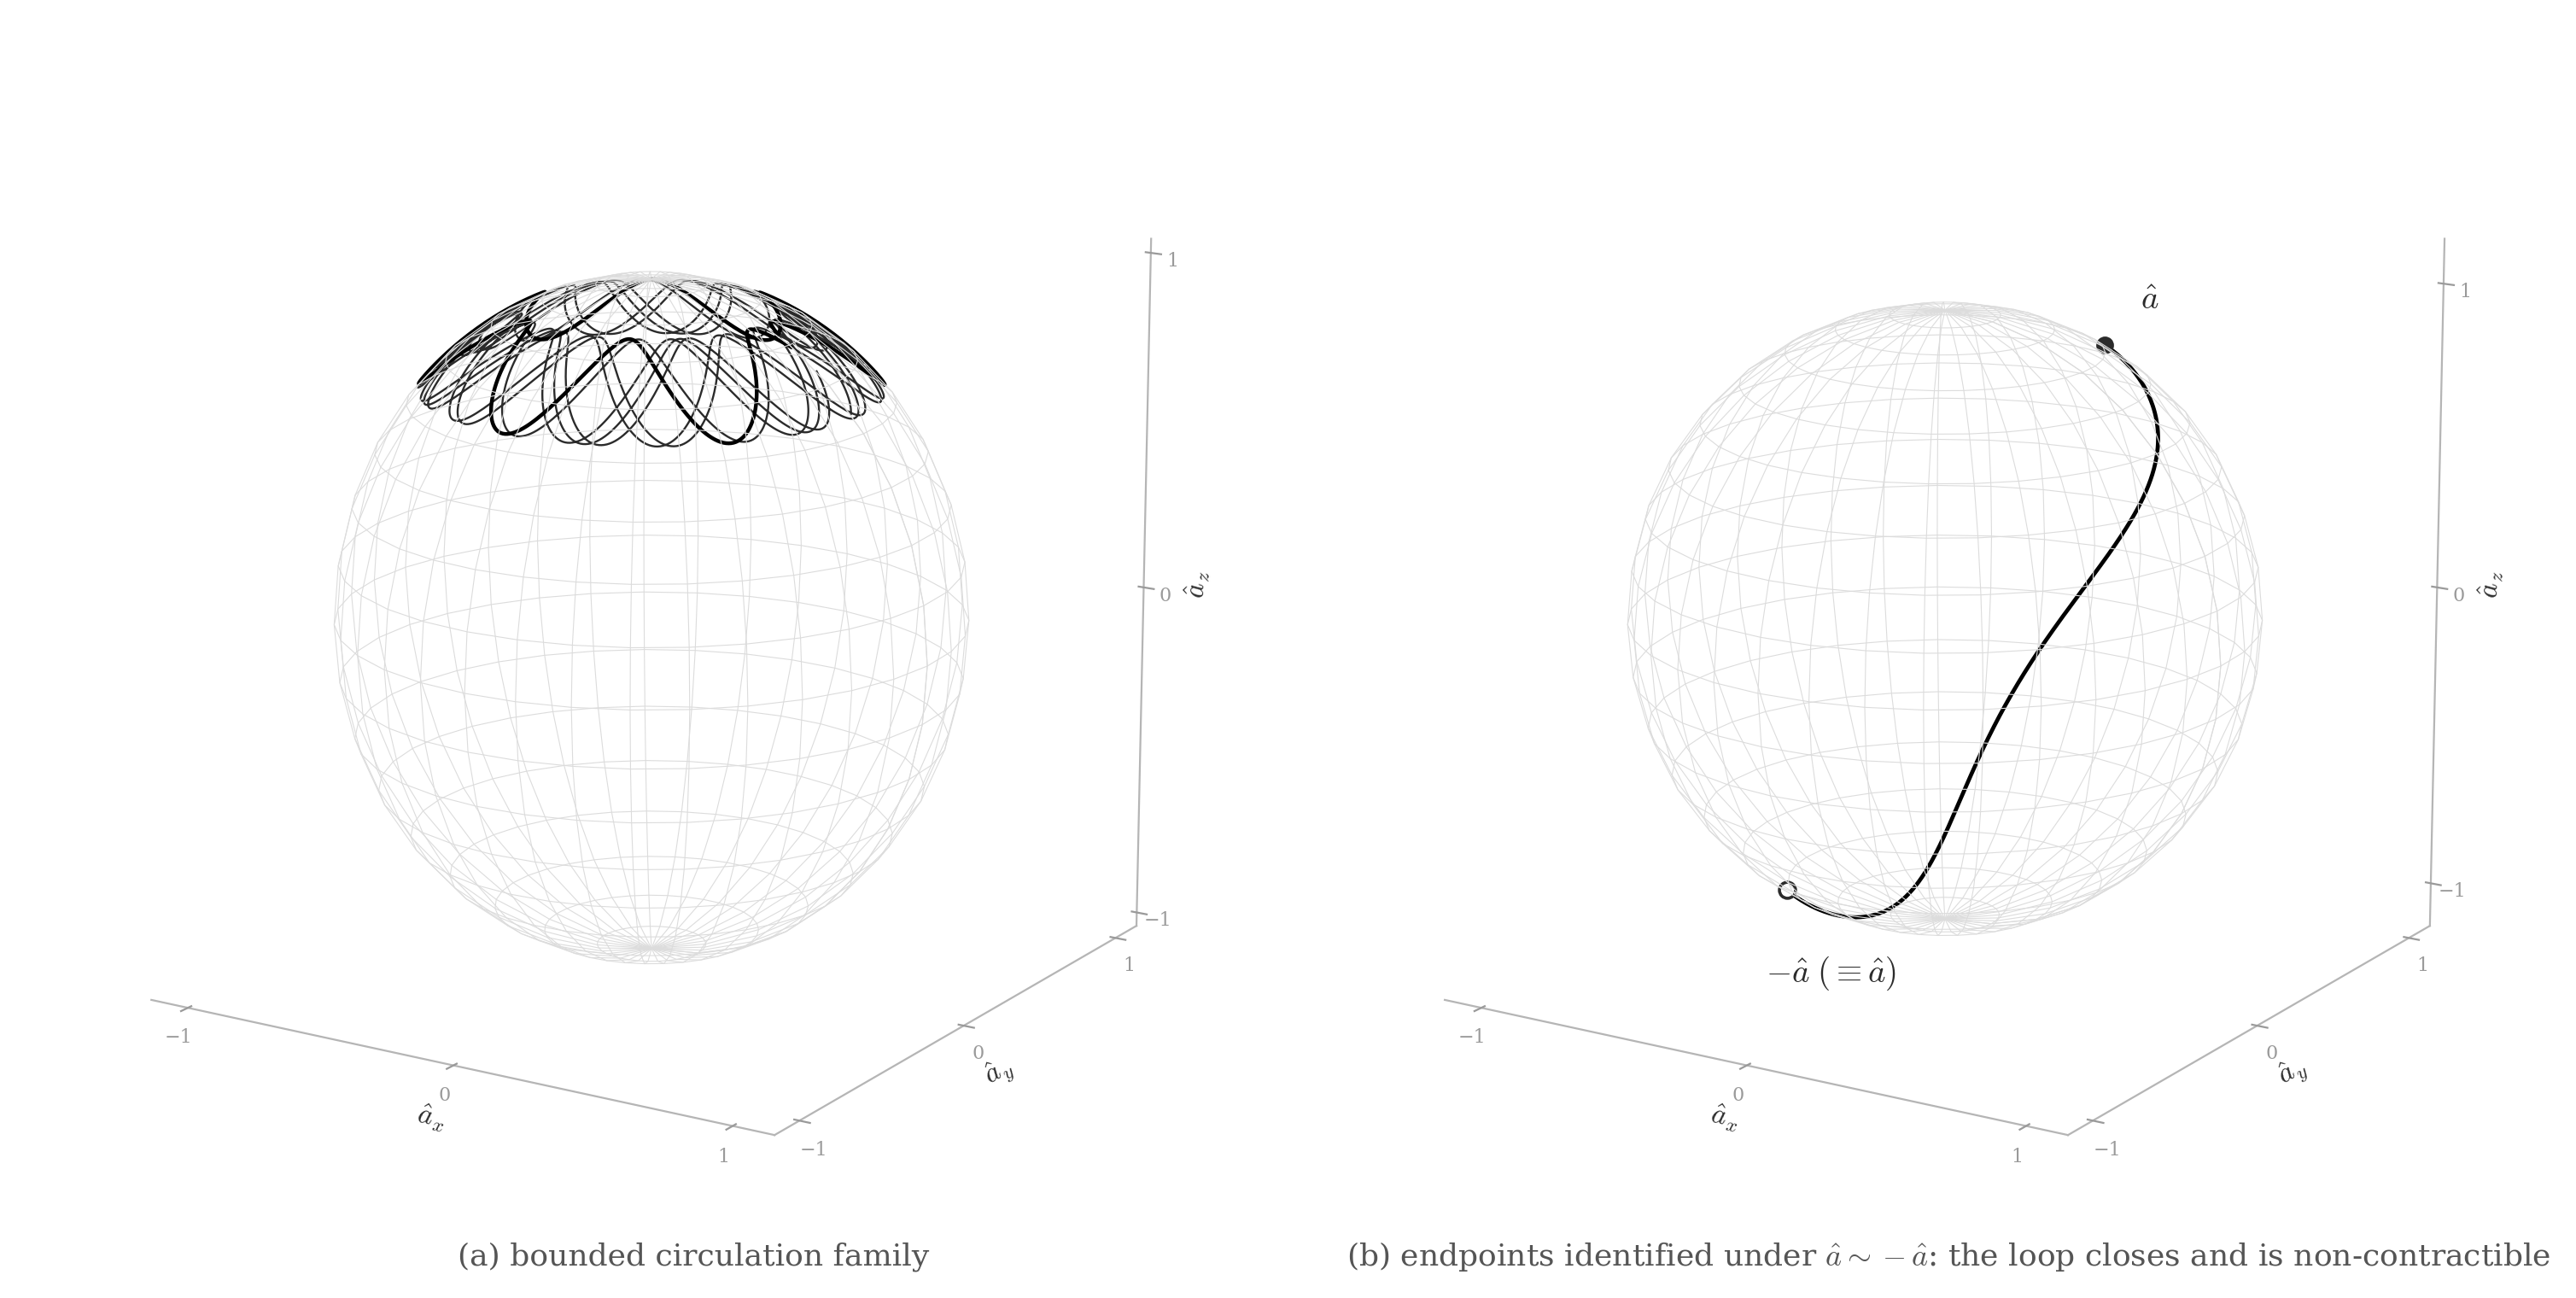
\includegraphics[width=0.72\linewidth]{fig_spin_axis_proxy_noncontractible.png}
\captionsetup{justification=raggedright,singlelinecheck=false}
\caption{\textbf{Non-contractible circulation sector (spin-axis proxy).}
The unit spin-axis proxy
\[
\hat{\mathbf a}(\tau)
=
\frac{
\mathbf x(\tau)\times\dot{\mathbf x}(\tau)
}{
\|\mathbf x(\tau)\times\dot{\mathbf x}(\tau)\|
}
\]
traces a bounded family of closed loops in the chosen reconstruction;
panel (a), with one representative loop drawn heavier. The circulation
is represented inside a circulation-supporting sector
\(\mathcal M_E\subseteq B_E\). Panel (b): under the declared
antipodal identification \(\hat{\mathbf a}\sim-\hat{\mathbf a}\)
the representation space is the real projective plane, and a path
joining an axis to its antipode closes into a loop whose class is
genuinely nontrivial; its double traversal is contractible, the
\(\mathbb Z/2\) loop structure of \(\mathbb{RP}^2\). The sphere
drawn is a representation surface only, and without the identification
it is simply connected: nontriviality lives in the identified space and
in the declared loop-equivalence structure on \(\mathcal M_E\), not
in the sphere. Nontrivial loop classes provide a structural witness of
sequencing-stable circulation within admissible structure rather than
literal rotation in physical space.}
\label{fig:spin_axis_proxy_noncontractible}
\end{figure}

\paragraph{Why non-contractibility matters.}

If every admissible loop class in \(\mathcal M_E\) can be removed under
the declared loop-equivalence structure, then any candidate spin proxy
can be erased without leaving the circulation-supporting sector. In
that case, persistence fails by structure.

Outside a circulation-supporting sector, a spin proxy is not merely
unstable; it is undefined as a structural witness.

The existence of non-removable circulation classes is therefore what
licenses a persistent spin-like description within the toy model.

\paragraph{Bridge to the explicit surrogate.}

The loop-class condition above is a structural statement involving
\(B_E\), \(\mathcal M_E\), and the declared loop family
\(\mathcal L_E(\mathcal M_E)\). It may use \(\Gamma_E\) only when a
model explicitly derives the loop family from the connectivity
structure.

The chart-level surrogates introduced in the following subsection do
not generate this structure. Instead, they provide analyst-chosen
witnesses of local contraction-like representation and circulation under
state-independent parameters.

The nontrivial loop organization is carried by the declared admissible
sector and its loop-equivalence structure. The surrogate flow merely
provides a convenient representation of that organization.

\paragraph{What this does not claim.}

This toy model does not claim that spin is literal rotation of a
point-like body, nor that angular momentum must be defined relative to
an external spacetime frame.

It does not introduce a primitive torque law, microscopic spin
mechanism, state-conditioned update process, primitive topology, or
basin dynamics.

Any effective interaction between a spin proxy and an external field is
interpreted as context re-indexing or as a model-specific reshaping of
admissible structure. It is not a state-conditioned steering law.

Geometric-phase and orientation-based models provide useful
interpretive parallels~\cite{BarutZanghi1984,Hestenes1990,Berry1984},
but none are adopted as axioms or microscopic commitments.

\subsubsection{Toy Basin Flow: Confinement and Circulation}
\label{toy:spin_proxy:basin_flow}

\paragraph{What this surrogate is.}

This surrogate is an analyst-chosen chart-level witness for the
coexistence of contraction-like confinement and circulation within a
circulation-supporting sector
\[
\mathcal M_E
\subseteq
B_E
\subseteq
\mathcal A(E).
\]

It does not generate basin structure, connectivity structure, topology,
neighbourhood structure, measure structure, or loop classes. Those
objects are specified independently through the structural layer of the
framework.

The surrogate exists solely to provide an explicit representation of
local contraction together with persistent circulation.

The parameter \(\tau\) is an ordering or reconstruction label rather
than physical time. All surrogate parameters are indexed only by the
fixed classical context \(E\), in accordance with NS1. Any
\(\tau\)-dependence is permitted only as exogenous classical-context
drift, represented by re-indexing through \(E\).

\paragraph{The surrogate equation.}

Fix an analyst-chosen coordinate
\[
\mathbf{x}(\tau)\in\mathbb R^d,
\]
where
\[
d=d(E),
\qquad
\tau\in\mathbb R_{\geq 0},
\qquad
\dot{\mathbf{x}}
:=
\frac{d\mathbf{x}}{d\tau}.
\]

Let
\[
M=M(E)\in\mathbb N.
\]
Define
\begin{equation}
\dot{\mathbf{x}}
=
-k(E)\mathbf{x}
+
\sum_{m=1}^{M}
\omega_m(E)J_m(E)\mathbf{x},
\qquad
k(E)>0,
\qquad
J_m(E)^\top=-J_m(E).
\label{eq:toy_basin_flow_multifactor}
\end{equation}

The parameter \(k(E)\) acts as a contraction-strength proxy. The skew
operators \(J_m(E)\) represent circulation geometry within the chosen
chart. The coefficients \(\omega_m(E)\) weight the relative contribution
of the circulation components.

The two terms play distinct representational roles:
\begin{itemize}
\item \(-k(E)\mathbf{x}\) produces uniform radial contraction;
\item \(\sum_m\omega_m(E)J_m(E)\mathbf{x}\) produces circulation.
\end{itemize}

Together they provide a chart-level witness of contraction together
with circulation. They do not define a physical force law, torque law,
basin dynamics, or microscopic spin model.

\paragraph{Confinement: Lyapunov witness.}

Define
\[
V(\mathbf{x})
=
\frac12
\|\mathbf{x}\|^2.
\]

Since each \(J_m(E)\) is skew-symmetric,
\[
\mathbf{x}^\top J_m(E)\mathbf{x}
=
0
\]
for all \(\mathbf{x}\). Therefore
\begin{align}
\dot V
&=
\mathbf{x}^\top\dot{\mathbf{x}}
\nonumber\\
&=
\mathbf{x}^\top
\Bigl(
-k(E)\mathbf{x}
+
\sum_m
\omega_m(E)J_m(E)\mathbf{x}
\Bigr)
\nonumber\\
&=
-k(E)\|\mathbf{x}\|^2
=
-2k(E)V.
\label{eq:toy_basin_lyapunov}
\end{align}

Hence
\begin{equation}
\|\mathbf{x}(\tau)\|
=
\|\mathbf{x}(0)\|
e^{-k(E)\tau}.
\label{eq:toy_basin_norm_decay}
\end{equation}

The surrogate therefore exhibits strict radial contraction together
with circulation.

\paragraph{Important limitation.}

The surrogate flow does not generate, define, or preserve the
non-contractible loop classes introduced in
Sec.~\ref{toy:spin_proxy:noncontractible}.

Those structural features belong to the circulation-supporting sector
\(\mathcal M_E\), together with its declared loop-equivalence structure.
They are not produced by Eq.~\eqref{eq:toy_basin_flow_multifactor}.

The surrogate merely provides a convenient chart-level witness of
contraction plus circulation.

\begin{figure}[t]
\centering
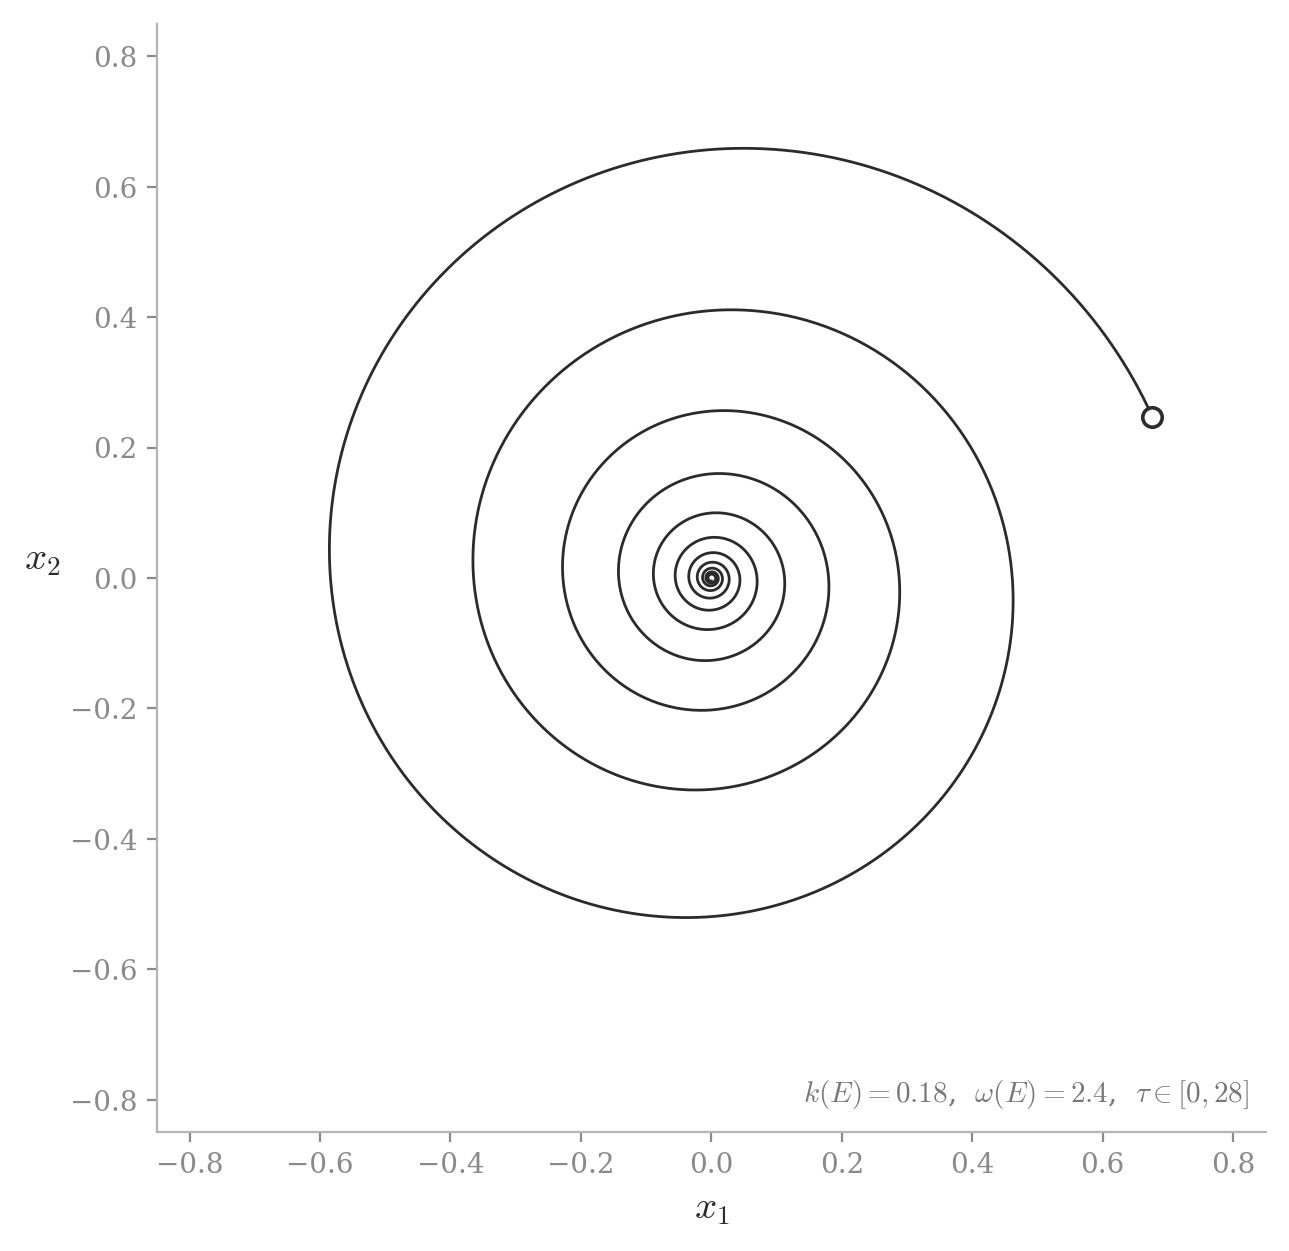
\includegraphics[width=0.62\linewidth]{fig_toy_basin_flow_spiral.png}
\captionsetup{justification=raggedright,singlelinecheck=false}
\caption{\textbf{Toy basin flow surrogate: contraction with circulation.}
The curve is a solution of Eq.~\eqref{eq:toy_basin_flow_multifactor}
in an analyst-chosen two-dimensional chart plane, with the parameters
stated in the panel; the open marker is the initial condition. The
surrogate trajectory exhibits strict radial contraction together with
persistent circulation. The inward spiral reflects the spectrum of the
surrogate generator and serves only as a chart-level witness.
Non-contractible loop classes are supplied by the declared
circulation-supporting sector and are not generated by the surrogate
flow.}
\label{fig:toy_basin_flow_spiral}
\end{figure}

\paragraph{Multi-factor circulation.}

Define
\[
S(E)
:=
\sum_{m=1}^{M}
\omega_m(E)J_m(E).
\]

Since each \(J_m(E)\) is skew-symmetric,
\[
S(E)^\top=-S(E).
\]

For \(k(E)=0\), the operator \(S(E)\) generates norm-preserving
rotations on its invariant subspaces. For \(k(E)>0\), circulation
persists while the radius contracts.

This is the minimal chart-level witness of contraction together with
circulation.

\paragraph{Stability and spectrum.}

Equation~\eqref{eq:toy_basin_flow_multifactor} has the form
\[
\dot{\mathbf{x}}
=
A(E)\mathbf{x},
\qquad
A(E)
=
-k(E)I
+
S(E).
\]

Because
\[
\frac{A(E)+A(E)^\top}{2}
=
-k(E)I,
\]
the symmetric part of \(A(E)\) is strictly negative definite.

Moreover, since \(S(E)\) is real skew-symmetric, its eigenvalues are
purely imaginary, possibly including zero. Therefore every eigenvalue
\(\lambda\) of
\[
A(E)=-k(E)I+S(E)
\]
satisfies
\[
\Re(\lambda)=-k(E)<0.
\]

The imaginary spectrum of \(S(E)\) determines the circulation rates.
Stability is therefore global and exponential~\cite{Khalil2002}.

\paragraph{Closed-form solution.}

Since \(-k(E)I\) commutes with \(S(E)\),
\[
\mathbf{x}(\tau)
=
e^{(-k(E)I+S(E))\tau}
\mathbf{x}(0)
=
e^{-k(E)\tau}
e^{S(E)\tau}
\mathbf{x}(0).
\]

The solution is a composition of uniform contraction and rigid
multi-factor rotation.

\paragraph{3D specialization.}

For \(d=3\), every skew-symmetric operator \(S(E)\) can be written
uniquely as
\[
S(E)
=
[\boldsymbol{\Omega}(E)\times]
\]
for some
\[
\boldsymbol{\Omega}(E)\in\mathbb R^3.
\]

The surrogate then becomes
\begin{equation}
\dot{\mathbf{x}}
=
-k(E)\mathbf{x}
+
\boldsymbol{\Omega}(E)\times\mathbf{x}.
\label{eq:toy_basin_flow}
\end{equation}

\paragraph{NS1 compatibility.}

All parameters
\[
k(E),
\qquad
\{\omega_m(E)\},
\qquad
\{J_m(E)\},
\qquad
\boldsymbol{\Omega}(E)
\]
are fixed context descriptors indexed only by \(E\).

No state-conditioned retuning, outcome-dependent update, or
state-dependent generator selection is introduced. The surrogate also
does not retune
\[
\Gamma_E,
\qquad
\mathcal N_E,
\qquad
\mu_E.
\]

The construction remains a chart-level witness and not a dynamical
model.

\subsubsection{Axis Witnesses, Inclination Invariants, and Reconstruction Re-Indexing}
\label{toy:spin_proxy:axis_precession}

\paragraph{Why axis witnesses are needed.}

The surrogate flow of
Sec.~\ref{toy:spin_proxy:basin_flow}
provides a chart-level witness of contraction together with circulation.
It does not, by itself, define a primitive spin axis or physical
orientation.

In spin-like descriptions, orientation matters. This section introduces
reconstruction-level witnesses that summarize the orientation of
circulation within the surrogate representation.

Under fixed context \(E\), the generator-defined circulation direction
is fixed. Apparent axis drift or ``precession'' arises only through
context re-indexing or reconstruction-frame change, not through any
within-model dynamical process.

All objects introduced here are diagnostic only. Nothing in this
section constitutes a torque law, microscopic spin mechanism, spacetime
rotation claim, admissible update rule, or state-conditioned steering
mechanism.

\paragraph{Trajectory-defined circulation witness.}

For the 3D surrogate
\eqref{eq:toy_basin_flow},
define the trajectory-defined circulation witness
\begin{equation}
\mathbf a(\tau)
:=
\mathbf x(\tau)
\times
\dot{\mathbf x}(\tau),
\label{eq:toy_axis_proxy}
\end{equation}
wherever
\[
\mathbf x(\tau)\neq \mathbf 0.
\]

If
\[
\boldsymbol{\Omega}(E)=\mathbf 0,
\]
then
\[
\dot{\mathbf x}
=
-k(E)\mathbf x,
\]
and therefore
\[
\mathbf a(\tau)\equiv \mathbf 0.
\]
In that case no circulation witness is licensed within the surrogate
chart.

Substituting
\[
\dot{\mathbf x}
=
-k(E)\mathbf x
+
\boldsymbol{\Omega}(E)\times\mathbf x
\]
gives
\begin{equation}
\mathbf a(\tau)
=
\mathbf x(\tau)
\times
\bigl(
\boldsymbol{\Omega}(E)
\times
\mathbf x(\tau)
\bigr),
\label{eq:toy_axis_proxy_triple}
\end{equation}
because the contraction contribution satisfies
\[
\mathbf x(\tau)\times[-k(E)\mathbf x(\tau)]
=
\mathbf 0.
\]

The resulting object provides an oriented trajectory-level witness of
circulation structure without introducing torques, forces, microscopic
generators, or physical rotation of a body.

The witness \(\mathbf a(\tau)\) should not be confused with a primitive
axis. It depends on the chosen chart trajectory \(\mathbf x(\tau)\).
The fixed context \(E\) fixes the generator direction
\(\boldsymbol{\Omega}(E)\), not necessarily the instantaneous direction
of every trajectory-defined witness.

\begin{figure}[t]
\centering
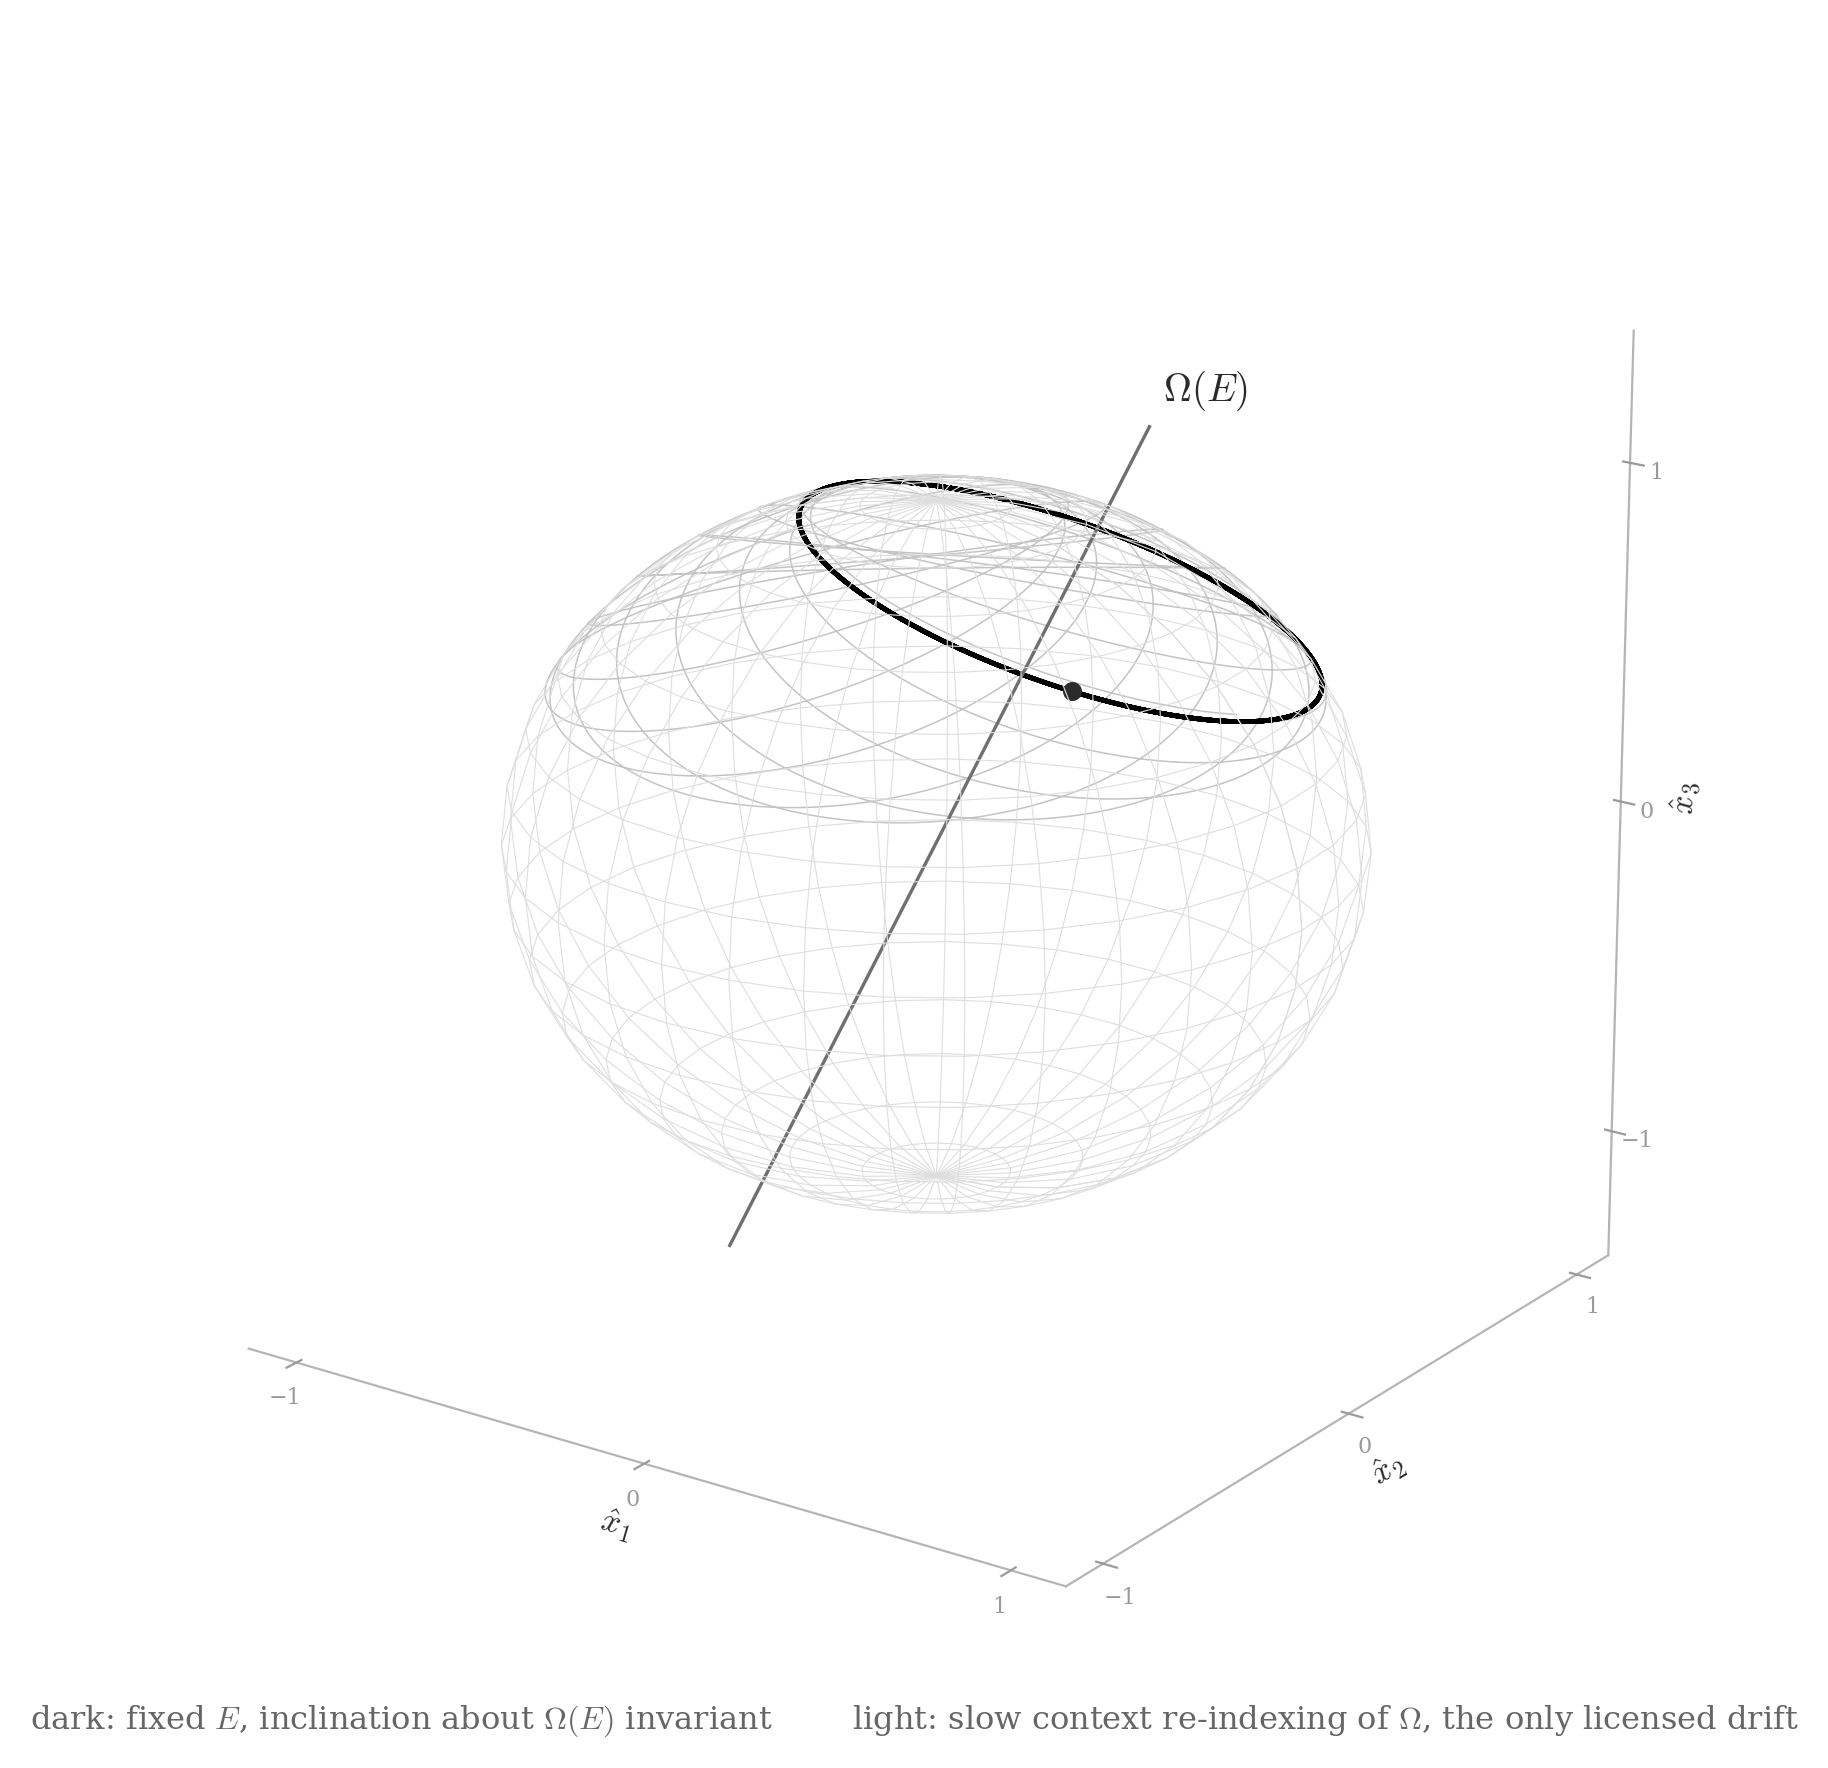
\includegraphics[width=0.66\linewidth]{fig_spin_proxy_trajectory_fixed_radius_sphere.png}
\captionsetup{justification=raggedright,singlelinecheck=false}
\caption{\textbf{Trajectory witness for circulation orientation.}
A reconstruction-level witness derived from the surrogate trajectory
projected onto a fixed-radius sphere. The circulation witness
\[
\mathbf a(\tau)=\mathbf x(\tau)\times\dot{\mathbf x}(\tau)
\]
summarizes trajectory-level orientation within the chart representation.
Under fixed context \(E\), the generator-defined circulation direction
\(\boldsymbol{\Omega}(E)\) is fixed, and the inclination angle between
\(\mathbf x(\tau)\) and \(\boldsymbol{\Omega}(E)\) remains invariant:
the dark curve, a numerically integrated solution of
Eq.~\eqref{eq:toy_basin_flow} projected to unit radius, traces a circle
of constant inclination about the drawn axis. Apparent drift of the
generator-defined axis arises only through context re-indexing or
reconstruction-frame change; the light band shows the same witness under
slow re-indexing of \(\boldsymbol{\Omega}\).}
\label{fig:spin_proxy_trajectory_fixed_radius}
\end{figure}

\paragraph{Generator-defined orientation witness.}

For the 3D surrogate,
\[
S(E)
=
[\boldsymbol{\Omega}(E)\times].
\]

Whenever
\[
\boldsymbol{\Omega}(E)\neq\mathbf 0,
\]
define
\begin{equation}
\widehat{\mathbf a}_{\Omega}(E)
:=
\frac{\boldsymbol{\Omega}(E)}
{\|\boldsymbol{\Omega}(E)\|}
\in
\mathbb S^2.
\label{eq:toy_axis_unit_proxy}
\end{equation}

This object is not a primitive axis variable and does not enter any
admissible update rule. It is a reconstruction witness summarizing the
orientation of the circulation geometry represented by the surrogate.

The trajectory-defined witness may vanish for special trajectories, for
example when
\[
\mathbf x(\tau)\parallel\boldsymbol{\Omega}(E),
\]
whereas the generator-defined witness remains well-defined whenever
\(\boldsymbol{\Omega}(E)\neq\mathbf 0\).

\paragraph{Axis identity and inclination invariant.}

Using the vector triple-product identity,
\begin{equation}
\mathbf a(\tau)
=
\|\mathbf x(\tau)\|^2
\boldsymbol{\Omega}(E)
-
\bigl(
\boldsymbol{\Omega}(E)\cdot
\mathbf x(\tau)
\bigr)
\mathbf x(\tau).
\label{eq:toy_axis_proxy_identity}
\end{equation}

For \(\mathbf x(\tau)\neq\mathbf 0\) and
\(\boldsymbol{\Omega}(E)\neq\mathbf 0\),
\[
\mathbf a(\tau)=\mathbf 0
\]
if and only if
\[
\mathbf x(\tau)\parallel\boldsymbol{\Omega}(E).
\]

For generic initial conditions,
\[
\|\mathbf a(\tau)\|
=
\|\boldsymbol{\Omega}(E)\|\,
\|\mathbf x(\tau)\|^2
\sin\theta,
\]
where
\[
\theta
:=
\angle
\bigl(
\mathbf x(\tau),
\boldsymbol{\Omega}(E)
\bigr).
\]

Under fixed context \(E\), both \(k(E)\) and
\(\boldsymbol{\Omega}(E)\) are constant. Since
\[
\frac{d}{d\tau}
\bigl(
\boldsymbol{\Omega}(E)\cdot\mathbf x
\bigr)
=
-k(E)
\bigl(
\boldsymbol{\Omega}(E)\cdot\mathbf x
\bigr),
\]
and
\[
\frac{d}{d\tau}
\|\mathbf x\|
=
-k(E)\|\mathbf x\|,
\]
the ratio
\[
\frac{
\boldsymbol{\Omega}(E)\cdot\mathbf x
}{
\|\mathbf x\|
}
\]
is constant.

Hence the inclination angle \(\theta\) between
\(\mathbf x(\tau)\) and \(\boldsymbol{\Omega}(E)\) is invariant.

Within the surrogate representation, the generator-defined circulation
direction does not precess under fixed context. The
trajectory-defined witness \(\mathbf a(\tau)\), however, remains a
chart-dependent trajectory witness and should not be confused with a
primitive axis.

Since
\[
\|\mathbf x(\tau)\|
=
\|\mathbf x(0)\|
e^{-k(E)\tau},
\]
it follows that
\begin{equation}
\|\mathbf a(\tau)\|
\propto
e^{-2k(E)\tau}.
\label{eq:toy_axis_mag_decay}
\end{equation}

This decay reflects chart-level contraction and not a torque effect.

\paragraph{Context re-indexing and apparent precession.}

Introduce a family of contexts
\[
\{E_\lambda\}_{\lambda\in\Lambda}
\]
with
\[
\boldsymbol{\Omega}_\lambda
:=
\boldsymbol{\Omega}(E_\lambda).
\]

Given an externally specified bookkeeping protocol
\[
\lambda=\lambda(\tau),
\]
define
\[
\boldsymbol{\Omega}(\tau)
:=
\boldsymbol{\Omega}
\bigl(
E_{\lambda(\tau)}
\bigr).
\]

No physical ordering mechanism is asserted by this notation.

Whenever
\[
\boldsymbol{\Omega}(\tau)\neq\mathbf 0,
\]
define
\begin{equation}
\widehat{\mathbf a}_{\Omega}(\tau)
:=
\frac{
\boldsymbol{\Omega}(\tau)
}{
\|\boldsymbol{\Omega}(\tau)\|
}.
\label{eq:toy_axis_proxy_drift}
\end{equation}

Any variation of
\[
\widehat{\mathbf a}_{\Omega}(\tau)
\]
is, by construction, a consequence of context re-indexing.

Within SSAF this is the intended interpretation of apparent
``precession'': a reconstruction effect arising from changes in context
indexing, rather than a dynamical rotation law.

\paragraph{Co-rotating representations.}

Let
\[
R(\tau)\in SO(3)
\]
be an analyst-chosen reconstruction frame and define
\[
\mathbf y(\tau)
:=
R(\tau)^\top
\mathbf x(\tau).
\]

Let
\(\boldsymbol{\omega}_R(\tau)\) denote the angular velocity associated
with the chosen representation, expressed in the reconstructed frame.
Define it by
\[
R(\tau)^\top\dot R(\tau)
=
[\boldsymbol{\omega}_R(\tau)\times],
\]
equivalently,
\[
\dot R(\tau)
=
R(\tau)[\boldsymbol{\omega}_R(\tau)\times].
\]

Then
\begin{align}
\dot{\mathbf y}
&=
R^\top\dot{\mathbf x}
-
R^\top\dot R\,\mathbf y
\nonumber\\
&=
-k(E)\mathbf y
+
\bigl(
\boldsymbol{\Omega}_R(\tau)
-
\boldsymbol{\omega}_R(\tau)
\bigr)
\times
\mathbf y,
\label{eq:toy_compensated_frame}
\end{align}
where
\[
\boldsymbol{\Omega}_R(\tau)
=
R(\tau)^\top
\boldsymbol{\Omega}(\tau).
\]

Choosing
\[
\boldsymbol{\omega}_R(\tau)
=
\boldsymbol{\Omega}_R(\tau)
\]
eliminates the circulation term and yields
\[
\dot{\mathbf y}
=
-k(E)\mathbf y.
\]

This demonstrates that the observed circulation depends on the chosen
reconstruction chart.

The co-rotating representation is therefore a bookkeeping choice and
not an admissible operation, physical mechanism, or dynamical process.

Its purpose is to emphasize that circulation orientation is represented
through reconstruction witnesses rather than through a fundamental axis
variable.

\subsubsection{Axis-Variance Diagnostics}
\label{toy:spin_proxy:variance_diag}

\paragraph{Purpose.}

The preceding sections established that under fixed context \(E\), the
generator-defined circulation direction is fixed, and that apparent
``precession'' is represented only through context re-indexing or
reconstruction-frame change.

This section introduces quantitative diagnostics for characterizing the
stability of circulation-orientation witnesses under such re-indexing.

The diagnostics are bookkeeping tools for reconstruction analysis. They
are not stochastic dynamics, measurement back-action, torque laws,
admissible operations, update mechanisms, or state-conditioned feedback
rules.

All averaging and variance calculations are performed over
analyst-chosen reconstruction windows.

\paragraph{Orientation witness.}

For the 3D surrogate~\eqref{eq:toy_basin_flow}, whenever
\[
\boldsymbol{\Omega}(\tau)\neq\mathbf 0,
\]
define
\begin{equation}
\widehat{\mathbf a}(\tau)
:=
\frac{
\boldsymbol{\Omega}(\tau)
}{
\|\boldsymbol{\Omega}(\tau)\|
}.
\label{eq:toy_axis_unit}
\end{equation}

Under fixed context \(E\), the orientation witness is constant:
\[
\widehat{\mathbf a}(\tau)
=
\widehat{\mathbf a}_{\Omega}(E).
\]

Any variation is permitted only through exogenous classical-context
drift or reconstruction re-indexing.

\paragraph{Angular deviation from a reference witness.}

Fix a reference orientation witness
\[
\widehat{\mathbf a}_{\mathrm{ref}},
\]
for example
\[
\widehat{\mathbf a}(\tau_0)
\]
at a chosen reconstruction point.

Define
\begin{equation}
\theta(\tau)
:=
\arccos
\!\Bigl(
\min
\bigl\{
1,
\max
\bigl\{
-1,
\widehat{\mathbf a}(\tau)
\cdot
\widehat{\mathbf a}_{\mathrm{ref}}
\bigr\}
\bigr\}
\Bigr).
\label{eq:toy_axis_angle}
\end{equation}

The clipping inside the arccosine is a numerical convention ensuring
that roundoff error does not push the inner product outside
\([-1,1]\). This quantity measures orientation drift relative to the
chosen reference witness.

\paragraph{Windowed variance: wobble index.}

For a reconstruction window
\[
W=[\tau_0,\tau_1],
\qquad
|W|=\tau_1-\tau_0>0,
\]
define
\[
\bar{\theta}_W
=
\frac{1}{|W|}
\int_{\tau_0}^{\tau_1}
\theta(\tau)\,d\tau,
\]
and
\begin{equation}
\mathrm{Var}_W(\theta)
=
\frac{1}{|W|}
\int_{\tau_0}^{\tau_1}
\bigl(
\theta(\tau)
-
\bar{\theta}_W
\bigr)^2
d\tau.
\label{eq:toy_theta_variance}
\end{equation}

This diagnostic quantifies orientation drift produced by context
re-indexing. Values near zero indicate reconstruction stability. Larger
values indicate stronger context-dependent variation.

\paragraph{Vector concentration diagnostic.}

Define the window-averaged orientation witness
\begin{equation}
\bar{\mathbf a}_W
=
\frac{1}{|W|}
\int_{\tau_0}^{\tau_1}
\widehat{\mathbf a}(\tau)\,d\tau.
\label{eq:toy_axis_mean}
\end{equation}

The corresponding concentration diagnostic is
\begin{equation}
\mathcal V_W
:=
1
-
\|
\bar{\mathbf a}_W
\|.
\label{eq:toy_axis_vector_variance}
\end{equation}

Since \(\widehat{\mathbf a}(\tau)\) is unit-length wherever it is
defined, the triangle inequality gives
\[
0
\leq
\mathcal V_W
\leq
1.
\]

The value \(\mathcal V_W=0\) occurs for a perfectly stable orientation
witness over the window. Larger values indicate greater dispersion of
orientation witnesses over the chosen reconstruction window.

\paragraph{Relation to admissibility concentration.}

The quantity \(\mathcal V_W\) is a reconstruction-level concentration
diagnostic and should not be confused with the admissibility measure
\(\mu_E\).

The admissibility measure \(\mu_E\) characterizes structural weight or
concentration of admissible regions within \(\mathcal A(E)\). The
present diagnostic characterizes concentration of orientation witnesses
within an analyst-chosen reconstruction window.

The two notions are conceptually distinct, although future
model-specific constructions may relate them.

\paragraph{Optional trajectory witness.}

If a trajectory-defined circulation witness is desired, define
\begin{equation}
\mathbf c(\tau)
:=
\mathbf x(\tau)
\times
\dot{\mathbf x}(\tau),
\qquad
d=3.
\label{eq:toy_circ_witness}
\end{equation}

Under fixed \(\boldsymbol{\Omega}\) and the invariant-subspace
condition
\[
\mathbf x(\tau_0)\cdot\boldsymbol{\Omega}=0,
\]
which is preserved under the surrogate flow, one obtains
\begin{equation}
\mathbf c(\tau)
=
\|\mathbf x(\tau)\|^2
\boldsymbol{\Omega}.
\label{eq:toy_circ_witness_parallel}
\end{equation}

Hence \(\mathbf c(\tau)\) remains parallel to the generator-defined
orientation witness and decays as
\[
e^{-2k\tau}.
\]

\paragraph{Separating orientation drift from contraction.}

For the ideal fixed-context surrogate,
\[
\|\mathbf c(\tau)\|
\propto
e^{-2k\tau}.
\]

If exogenous context drift permits
\[
k=k(\tau),
\]
and if \(\|\mathbf c(\tau)\|>0\) on the window, define the unregularized
log-magnitude residual
\begin{equation}
r_0(\tau)
:=
\frac{d}{d\tau}
\log
\|\mathbf c(\tau)\|
+
2k(\tau).
\label{eq:toy_axis_mag_residual_unregularized}
\end{equation}

For the ideal surrogate with
\[
\frac{d}{d\tau}\log\|\mathbf c(\tau)\|
=
-2k(\tau),
\]
one has
\[
r_0(\tau)\equiv 0.
\]

For numerical use near zeros of \(\mathbf c\), one may instead use the
regularized diagnostic
\begin{equation}
r_{\varepsilon}(\tau)
:=
\frac{d}{d\tau}
\log
\bigl(
\|\mathbf c(\tau)\|
+
\varepsilon_{\mathrm{mag}}
\bigr)
+
2k(\tau),
\qquad
\varepsilon_{\mathrm{mag}}>0.
\label{eq:toy_axis_mag_residual}
\end{equation}

The regularized residual need not vanish exactly, because the
regularizer changes the logarithmic derivative. It is a numerical
stability device, not a new structural object.

Deviation of \(r_0\) from zero, or persistent deviation of
\(r_{\varepsilon}\) beyond regularization effects, indicates context
variation beyond simple contraction-rate change. This remains a
diagnostic quantity and not a mechanism.

\paragraph{NS1 hygiene.}

All reconstruction windows, reference choices, and context-drift
families
\[
k(\tau),
\qquad
\boldsymbol{\Omega}(\tau)
\]
are specified externally through the classical context or reconstruction
protocol.

No diagnostic is permitted to retune parameters as a function of
\(\rho\), outcomes, ensemble decompositions, or state-derived
statistics. The diagnostics also do not retune
\[
\Gamma_E,
\qquad
\mathcal N_E,
\qquad
\mu_E.
\]

\paragraph{Summary.}

Apparent wobble and precession are represented solely through
context-dependent variation of the orientation witness
\(\widehat{\mathbf a}(\tau)\), or through reconstruction-frame change.

The variance diagnostics above quantify reconstruction stability while
remaining fully consistent with NS1. No torque law, microscopic
mechanism, state-conditioned feedback process, or admissible update
operation is introduced.

\subsection{Toy Model: Non-Total Structural Ordering Without Dynamics}
\label{toy:nontotal_ordering}

\noindent\emph{Axiom target:} Axiom~0 (Emergent Sequencing).

\paragraph{Axiom unit test: pass condition.}

Fix a classical context \(E\). The framework must admit a well-defined
notion of structural ordering that is \emph{not} total and is
\emph{not} reducible to dynamics, rates, transport, temporal succession,
or a privileged global chain.

Ordering assertions must be licensed solely by declared admissibility
and prerequisite constraints under fixed \(E\). Where no such constraint
is licensed, ordering claims are \emph{undefined}, not merely unknown.

Any attempt to restore total order by introducing state-conditioned
rules, outcome-based repair, hidden sequencing, or a privileged
scheduler violates SSAF guardrails.

\paragraph{Scope.}

This toy introduces no evolution law, generator, time parameter, rate,
selection rule, transport mechanism, or update map. The only
mathematical content is a declared prerequisite relation on a finite set
of addressability classes under fixed context \(E\).

\paragraph{What \(\prec_E\) is not.}

Do not read \(\prec_E\) as temporal succession, causation, transport,
physical evolution, or a process from one class to another. No
within-toy mechanism chooses between incomparable branches. No
state-conditioned retuning, retro-addressability, or
outcome-conditioned completion is introduced.

\subsubsection{Setup}
\label{toy:nontotal_ordering:setup}

\paragraph{Addressability classes.}

Fix \(E\) and an observational equivalence relation \(\sim_E\) on
\(\Phi\). Let
\[
Q_E := \Phi/{\sim_E}
\]
denote the set of \(E\)-indexed addressability classes.

\paragraph{Admissibility predicate on classes.}

A class \(K\in Q_E\) is \emph{admissible under \(E\)} iff it has at
least one admissible representative:
\begin{equation}
\mathrm{Adm}_E(K)
\;:\Longleftrightarrow\;
K\cap\mathcal A(E)\neq\varnothing.
\label{eq:toy_class_admissible}
\end{equation}

This is a domain-of-definition predicate under fixed \(E\), not a
dynamical condition.

\paragraph{Prerequisite constraints.}

A prerequisite constraint is a declared structural licensing statement
of the form
\[
K\triangleleft_E L,
\]
read as:
\begin{quote}
\emph{Any description that licenses \(L\) as admissible is structurally
committed to licensing \(K\) as an admissibility prerequisite.}
\end{quote}

The symbol \(\triangleleft_E\) is not material implication between
truth-values. It records a declared prerequisite constraint in the toy
language.

\subsubsection{Prerequisite Relation}
\label{toy:nontotal_ordering:relation}

\paragraph{Definition.}

Given a declared set of prerequisite constraints
\[
\mathcal P_E\subseteq Q_E\times Q_E,
\]
define \(\preceq_E\) to be the reflexive-transitive closure of
\(\mathcal P_E\). Define the strict prerequisite relation by
\begin{equation}
K\prec_E L
\;:\Longleftrightarrow\;
K\preceq_E L
\quad\text{and}\quad
K\neq L.
\label{eq:toy_prereq_relation}
\end{equation}

Thus \(K\prec_E L\) means that \(K\) is entailed as a structural
prerequisite for \(L\) by the declared prerequisite constraints and
transitivity. It is not a transition rule.

\paragraph{What \(K\prec_E L\) means in plain English.}

Under fixed \(E\), the statement \(K\prec_E L\) means:
\begin{quote}
\emph{Within this description, licensing \(L\) requires already
licensing \(K\) as a prerequisite class.}
\end{quote}

No notion of ``earlier/later,'' ``cause/effect,'' or ``process from
\(K\) to \(L\)'' is licensed. The relation is purely about which
class-admissibility claims are structurally prerequisite to others under
the same fixed context.

\paragraph{Formal properties.}

If the declared prerequisite constraints are acyclic, then
\(\prec_E\) is:

\begin{itemize}
\item \emph{Irreflexive:} \(K\not\prec_E K\).
\item \emph{Transitive:} if \(K\prec_E L\) and \(L\prec_E M\), then
\(K\prec_E M\).
\item \emph{Not total in general:} there need not exist a prerequisite
constraint comparing all distinct pairs.
\end{itemize}

The non-strict relation \(\preceq_E\) is the corresponding preorder;
when antisymmetry holds, it is a partial order.

\subsubsection{Toy Instance}
\label{toy:nontotal_ordering:instance}

\paragraph{Chosen classes.}

Select five distinct classes in \(Q_E\):
\[
X := \{A,B,C,D,F\}\subset Q_E.
\]
We use \(F\) instead of \(E\) to avoid collision with the context
symbol.

Assume these classes are admissible for the purposes of the toy:
\[
\mathrm{Adm}_E(A),\quad
\mathrm{Adm}_E(B),\quad
\mathrm{Adm}_E(C),\quad
\mathrm{Adm}_E(D),\quad
\mathrm{Adm}_E(F).
\]
Their admissibility alone does not create ordering relations.

\paragraph{Primitive prerequisite constraints.}

Declare only the following prerequisite constraints:
\begin{equation}
A\triangleleft_E C,
\qquad
B\triangleleft_E C,
\qquad
C\triangleleft_E D,
\qquad
B\triangleleft_E F.
\label{eq:toy_prereq_base}
\end{equation}

No other prerequisite constraints are assumed.

\paragraph{Derived consequences: transitivity only.}

From Eq.~\eqref{eq:toy_prereq_base} and transitivity:
\[
A\prec_E D,
\qquad
B\prec_E D.
\]

These are derived, not additional primitives. No further structure is
introduced.

\paragraph{Incomparability is structural.}

Several pairs are intentionally incomparable:
\[
A\ \text{vs.}\ B,
\qquad
A\ \text{vs.}\ F,
\qquad
D\ \text{vs.}\ F.
\]

These are not ``unknown orderings'' waiting to be resolved. The toy
supplies no licensed prerequisite constraint relating them, so claims
such as
\[
A\prec_E B,
\qquad
B\prec_E A,
\qquad
A\prec_E F,
\qquad
F\prec_E A
\]
are \emph{undefined} within the toy.

This is the central point: in SSAF, absence of a licensing constraint
does not mean ``we do not know yet.'' It means the claim has no defined
truth value in that description.

\subsubsection{No Privileged Chain and No Completion Mechanism}
\label{toy:nontotal_ordering:no_chain}

\paragraph{No privileged total ordering.}

This partial order supports multiple maximal chains, for example
\[
A\to C\to D,
\qquad
B\to C\to D,
\qquad
B\to F,
\]
without licensing any rule that selects among them.

Imposing a single global chain would require additional structure: a
scheduler, priority rule, clock, hidden ordering variable, or
outcome-conditioned completion rule. All such additions are outside
this toy's scope and outside SSAF's admissible operations under fixed
\(E\).

\begin{lemma}[No internal completion under fixed \(E\)]
\label{lem:toy_no_completion}
Within this toy, if neither \(K\prec_E L\) nor \(L\prec_E K\) is
entailed by the stipulated prerequisite constraints
Eq.~\eqref{eq:toy_prereq_base} together with transitivity, then the
ordering claim between \(K\) and \(L\) is undefined. Any attempt to
assign an order to such an incomparable pair introduces extra structure
not present in the toy.
\end{lemma}

\begin{proof}
The only licensed ordering facts are those entailed by the stipulated
constraints Eq.~\eqref{eq:toy_prereq_base} together with transitivity.
This generates a closed finite set of prerequisite facts.

If neither \(K\prec_E L\) nor \(L\prec_E K\) belongs to this generated
set, the toy provides no predicate value for that pair. The ordering
claim is therefore undefined in the toy language. There is no missing
information to be filled in; there is only structural absence of a
licensing constraint.

Any rule that assigns an order to an incomparable pair constitutes
additional structure beyond the stipulated constraints. If the rule is
a fixed tie-breaker, it is a completion mechanism, namely a hidden
scheduler or priority rule, not present in the toy's stated scope. If
the rule depends on \(\rho\), outcomes, ensemble decompositions, or
state-derived diagnostics, it is state-conditioned and violates NS1
discipline.

In either case, the repair comes from outside the fixed-\(E\)
description. Therefore undefined comparability cannot be repaired
internally.
\end{proof}

\subsubsection{Relation to SSAF Guardrails}
\label{toy:nontotal_ordering:guardrails}

\paragraph{What this unit test checks.}

This toy checks that SSAF supports non-total ordering as a structural
relation:

\begin{itemize}
\item ordering is not assumed total and is not identified with time;
\item admissibility alone does not create prerequisite ordering;
\item incomparability is treated as \emph{undefined}, not unresolved;
\item no state- or outcome-conditioned repair is introduced;
\item no transport, progression, or temporal narrative is smuggled in.
\end{itemize}

\paragraph{Summary.}

Meaningful ordering can be non-total and purely prerequisite-based.
Where \(\prec_E\) is not licensed, ordering claims are
\emph{undefined}, not merely unknown. Enforcing a single global chain
would require introducing forbidden additional structure.

The toy passes the unit test: non-total structural ordering is stable
and internally consistent under fixed \(E\).

\paragraph{Stability under coarse-graining.}

This toy works at the level of configurations, and that leaves one
natural objection open. A critic may grant configuration-level
incomparability while holding that configurations are over-fine: the
operationally meaningful objects are addressability classes, and on
passing to that quotient the ordering might complete, exposing the
incomparability above as an artifact of excessive resolution. The next
toy (Toy~\ref{toy:admissibility_entailment}) addresses this objection
directly. It runs the same discipline at the quotient level and shows
that no entailment relation among addressability classes completes the
order either
(Lemma~\ref{lem:toy_no_completion_entailment}). The two toys establish
a single claim at two levels of description: incomparability is stable
under coarse-graining.

\subsection{Toy Model: Admissibility Entailment Without Dynamics}
\label{toy:admissibility_entailment}

\noindent\emph{Axiom target:} Axiom~0 (Emergent Sequencing), at the quotient level.

\paragraph{Axiom unit test: pass condition.}

Fix a classical context \(E\). The framework must admit non-total
admissibility entailment among addressability classes without
introducing dynamics, rates, transport, temporal ordering, or any
internal completion mechanism.

Where entailment is not licensed by declared admissibility constraints
under fixed \(E\), comparability claims are \emph{undefined}. Any
attempt to repair undefinedness by state-conditioned rules,
outcome-based selection, hidden sequencing, or an internal completion
mechanism violates SSAF guardrails.

\paragraph{Relation to the previous toy.}

The preceding toy
(Sec.~\ref{toy:nontotal_ordering}) showed that structural ordering can
be non-total and undefined rather than merely unknown. This toy defends
that result at the level a critic would retreat to: it works with
addressability classes rather than configurations, asking which
class-admissibility claims are structurally committed to which other
claims under fixed \(E\), and shows that passing to the quotient does
not complete the order.

The result is therefore not merely the same point restated: it is the
configuration-level claim made stable under coarse-graining.
Non-totality persists, and undefined comparability cannot be internally
repaired at either level of description. The entailment
framing connects more directly to the spin proxy discussion, where the
question of which circulation modes are jointly licensed under fixed
\(E\) is central.

\paragraph{What this toy is not about.}

This toy does not describe ordering, evolution, branching in time,
rotation, torque, or transport. It describes domain-of-definition
constraints on which addressability classes can be simultaneously
licensed under a fixed descriptive context.

What appears as ``branching'' is non-total entailment. What appears as
``rotation'' or ``torque'' would be an illicit completion rule unless
explicitly introduced as exogenous context drift or external structure.

\subsubsection{Setup}
\label{toy:admissibility_entailment:setup}

\paragraph{Addressability classes.}

Fix an observational equivalence relation \(\sim_E\) on \(\Phi\), and
define
\[
Q_E:=\Phi/{\sim_E}
\]
as the set of \(E\)-indexed addressability classes.

\paragraph{Admissibility predicate.}

A class \(K\in Q_E\) is admissible under \(E\) iff it has at least one
admissible representative:
\begin{equation}
\mathrm{Adm}_E(K)
\;:\Longleftrightarrow\;
K\cap\mathcal A(E)\neq\varnothing.
\label{eq:toy_entailment_class_admissible}
\end{equation}

This is a domain-of-definition predicate only. It carries no temporal,
causal, dynamical, or ordering meaning.

\paragraph{Entailment constraints.}

An admissibility-entailment constraint is a declared structural
licensing statement of the form
\[
K\Rightarrow_E L,
\]
read as:
\begin{quote}
\emph{Licensing \(K\) as admissible under fixed \(E\) structurally
requires licensing \(L\) as admissible under the same fixed context.}
\end{quote}

The symbol \(\Rightarrow_E\) is not material implication between
truth-values. It records a declared entailment relation in the toy
language.

\subsubsection{Admissibility Entailment Relation}
\label{toy:admissibility_entailment:relation}

\paragraph{Definition.}

Given a declared set of admissibility-entailment constraints
\[
\mathcal Q_E\subseteq Q_E\times Q_E,
\]
define \(\Rightarrow_E\) to be the reflexive-transitive closure of
\(\mathcal Q_E\).

Thus
\[
K\Rightarrow_E L
\]
means that the admissibility of \(K\) structurally entails the
admissibility of \(L\) by the declared entailment constraints and
transitivity.

It is not a transition rule, time order, causal arrow, or dynamical
process.

\paragraph{What \(K\Rightarrow_E L\) means in plain English.}

Under fixed \(E\), the statement \(K\Rightarrow_E L\) means:
\begin{quote}
\emph{Within this description, any admissibility claim for \(K\)
requires the admissibility claim for \(L\).}
\end{quote}

No process takes \(L\) to \(K\), no transition is asserted, and no
choice is made. The relation states only which admissibility claims must
hold together under the declared fixed-\(E\) constraints.

\paragraph{Formal properties.}

If the declared entailment constraints are acyclic after quotienting
equivalent mutual entailments, then \(\Rightarrow_E\) is a preorder:
\begin{itemize}
\item \emph{Reflexive:} \(K\Rightarrow_E K\).
\item \emph{Transitive:} if \(K\Rightarrow_E L\) and
\(L\Rightarrow_E M\), then \(K\Rightarrow_E M\).
\item \emph{Not total in general:} there need not exist an entailment
constraint comparing all distinct pairs.
\end{itemize}

If antisymmetry is imposed on equivalence classes of mutual entailment,
the resulting relation is a partial order.

Non-comparability is structural undefinedness, not epistemic ignorance.

\subsubsection{Toy Instance}
\label{toy:admissibility_entailment:instance}

\paragraph{Chosen classes.}

Select five distinct classes
\[
X:=\{A,B,C,D,F\}\subset Q_E.
\]
Assume these classes are admissible for the purposes of the toy:
\[
\mathrm{Adm}_E(A),
\qquad
\mathrm{Adm}_E(B),
\qquad
\mathrm{Adm}_E(C),
\qquad
\mathrm{Adm}_E(D),
\qquad
\mathrm{Adm}_E(F).
\]
Their admissibility alone does not create entailment relations.

\paragraph{Primitive entailment constraints.}

Declare only:
\begin{equation}
C\Rightarrow_E A,
\qquad
C\Rightarrow_E B,
\qquad
D\Rightarrow_E C,
\qquad
F\Rightarrow_E B.
\label{eq:toy_entailment_base}
\end{equation}

No other entailment relations are licensed.

\paragraph{Derived entailments.}

From Eq.~\eqref{eq:toy_entailment_base} and transitivity:
\[
D\Rightarrow_E A,
\qquad
D\Rightarrow_E B.
\]
These are derived consequences, not additional primitive constraints.

\paragraph{Structural undefinedness.}

Pairs such as
\[
A\ \text{vs.}\ B,
\qquad
A\ \text{vs.}\ F,
\qquad
D\ \text{vs.}\ F
\]
admit no entailment in either direction under
Eq.~\eqref{eq:toy_entailment_base}.

These are not ``unknown'' relations. The toy supplies no licensing
constraint connecting them, so any comparison claim between such pairs
is \emph{undefined} within the toy language. Any attempt to rank,
compare, or complete them would add extra structure not present in the
fixed-\(E\) description.

\begin{lemma}[No internal entailment completion under fixed \(E\)]
\label{lem:toy_no_completion_entailment}
If neither \(K\Rightarrow_E L\) nor \(L\Rightarrow_E K\) is licensed by
the primitive entailments Eq.~\eqref{eq:toy_entailment_base} together
with transitivity, then comparability between \(K\) and \(L\) is
undefined. Any rule assigning an entailment direction to such an
undefined pair constitutes added structure.
\end{lemma}

\begin{proof}
The toy licenses only entailments derivable from
Eq.~\eqref{eq:toy_entailment_base} by reflexivity and transitivity.
This generates a closed finite set of facts.

If neither direction is derivable, the toy provides no entailment value
for that pair. The comparability claim is therefore undefined, not
missing; it is structurally absent.

Any additional rule that selects a direction introduces structure not
present in the toy. If the rule depends on \(\rho\), outcomes, ensemble
decompositions, or state-derived diagnostics, it is state-conditioned
and violates NS1. If the rule is a fixed tie-breaker, it is an external
scheduler or completion mechanism outside the toy's stated scope.

In either case, the repair comes from outside the fixed-\(E\)
description. No internal completion is licensed.
\end{proof}

\paragraph{Why ``torque'' language is a completion rule in disguise.}

In discussions of spin and circulation, it can be tempting to say that
an internal ``torque'' causes reorientation, precession, or branch
selection. Within SSAF, this is an illicit completion rule whenever it
assigns a direction to an undefined comparison using a within-model
mechanism not licensed by the fixed-\(E\) constraints.

Torque-like vocabulary may appear only as:
\begin{enumerate}[label=(\roman*), leftmargin=2.2em]
\item exogenous re-indexing of context,
\[
E\mapsto E(\tau);
\]
\item a reconstruction-frame choice;
\item explicitly added external structure.
\end{enumerate}

It is not a primitive internal mechanism at fixed \(E\).

\subsubsection{Unit-Test Takeaway}
\label{toy:admissibility_entailment:summary}

\paragraph{Summary.}

This toy demonstrates that what is often misread as ordering,
branching, rotation, or torque can arise purely as non-total
admissibility entailment under fixed context. Non-totality is
structural. Undefinedness is real.

Any internal ``torque'' or completion mechanism is an illegal repair
unless explicitly reframed as context drift, reconstruction-frame
choice, or external structure.

\subsection{Toy Model: Branching Prerequisite Structure Without Dynamics}
\label{toy:structural_nontotal_ordering}

\noindent\emph{Axiom target:} Axiom~0 (Emergent Sequencing), branching prerequisite structure.

\paragraph{Axiom unit test: pass condition.}

Under fixed classical context \(E\), a non-total branching prerequisite
structure must be representable purely via declared context-indexed
admissibility dependencies, without introducing dynamics, temporal
progression, causal influence, rates, probabilities, or
outcome-conditioned updating.

Where no prerequisite relation is licensed, ordering claims are
\emph{undefined} rather than repaired by any state- or
outcome-dependent rule. No retro-admissibility map is permitted.

\paragraph{How this toy differs from the previous two.}

The preceding ordering toys
(Secs.~\ref{toy:nontotal_ordering} and
\ref{toy:admissibility_entailment}) demonstrated non-total ordering and
non-total entailment on finite classes. This toy takes a more concrete
structural question: can admissibility constraints alone support a
\emph{branching} dependency, where two intermediate classes are each
required by a downstream class but are incomparable with each other?

The answer is yes. The branch is a structural fact about licensed
co-addressability under fixed \(E\), not a process that requires a
selection rule to resolve it.

\paragraph{What to avoid.}

This toy becomes misleading if one:

\begin{enumerate}[label=(\roman*), leftmargin=2.2em]

\item reads \(K_i\prec_E K_j\) as time evolution, transition, or causal
influence;

\item injects a hidden selection rule, such as rates, probabilities, or
outcome mechanisms, to ``resolve'' the branch;

\item assumes a within-ordering repair map that restores \(K_4\) after
loss of a prerequisite, i.e.\ retro-admissibility;

\item allows \(\prec_E\) to depend on \(\rho\), state diagnostics,
ensemble decompositions, or outcomes rather than on fixed \(E\);

\item treats the finite class diagram as a replacement for
envelope-closure, interface, compatibility, connectivity,
neighbourhood, or measure machinery. It is a skeleton only.

\end{enumerate}

\paragraph{Setup.}

Fix a classical context \(E\) and an observational equivalence relation
\[
\sim_E.
\]
Let
\[
Q_E:=\Phi/{\sim_E}
\]
denote the set of \(E\)-indexed addressability classes.

Choose four classes
\[
\{K_1,K_2,K_3,K_4\}\subset Q_E.
\]

A class \(K\in Q_E\) is \emph{admissible under \(E\)} iff it has at
least one admissible representative:
\[
K\cap\mathcal A(E)\neq\varnothing.
\]

This admissibility predicate supplies domain membership only. It does
not itself create prerequisite order.

\paragraph{Declared prerequisite constraints.}

Declare the following prerequisite constraints:

\begin{itemize}

\item \(K_2\) is licensed only if \(K_1\) remains licensed.

\item \(K_3\) is licensed only if \(K_1\) remains licensed.

\item \(K_4\) is licensed only if both \(K_2\) and \(K_3\) remain
licensed.

\end{itemize}

These are prerequisites, not causal influences. They constrain
co-addressability under fixed \(E\), but define no process.

The third constraint is the branching condition:
\[
K_4
\quad
\text{requires both}
\quad
K_2
\quad
\text{and}
\quad
K_3.
\]
Neither branch alone is sufficient.

\paragraph{Prerequisite relation.}

Let
\[
\mathcal P_E\subseteq Q_E\times Q_E
\]
be the declared prerequisite relation, with
\[
(K_i,K_j)\in\mathcal P_E
\]
read as:
\[
K_i\triangleleft_E K_j,
\]
meaning that \(K_i\) is a prerequisite for licensing \(K_j\).

Define \(\preceq_E\) as the reflexive-transitive closure of
\(\mathcal P_E\), and define the strict relation by
\begin{equation}
K_i\prec_E K_j
\;:\Longleftrightarrow\;
K_i\preceq_E K_j
\quad\text{and}\quad
K_i\neq K_j.
\label{eq:toy_branching_prereq_relation}
\end{equation}

Thus \(K_i\prec_E K_j\) means that \(K_i\) is entailed as a structural
prerequisite for \(K_j\) by the declared prerequisite constraints and
transitivity.

It is not a transition rule, time order, causal process, or dynamical
arrow.

\paragraph{Licensed prerequisite facts.}

Under fixed \(E\), stipulate:
\begin{equation}
K_1\triangleleft_E K_2,
\qquad
K_1\triangleleft_E K_3,
\qquad
K_2\triangleleft_E K_4,
\qquad
K_3\triangleleft_E K_4.
\label{eq:toy_branching_prereq_base}
\end{equation}

By transitivity, the following are derived:
\[
K_1\prec_E K_4.
\]

No relation between \(K_2\) and \(K_3\) is stipulated or derived.
Therefore neither
\[
K_2\prec_E K_3
\]
nor
\[
K_3\prec_E K_2
\]
is licensed in this toy.

The classes \(K_2\) and \(K_3\) are structurally incomparable: there is
no ordering claim between them that is defined within this description.

\paragraph{Two prerequisite supports, no preferred branch.}

The finite diagram contains two prerequisite supports feeding into
\(K_4\):
\[
K_1\to K_2\to K_4,
\qquad
K_1\to K_3\to K_4.
\]

These should not be read as two temporal routes, paths of motion, or
alternative histories. They are dependency supports inside a declared
prerequisite structure.

The toy provides no rule that selects between these supports, assigns a
rate, or imposes a clock. Any such selection would be additional
structure outside the toy's scope and outside what is licensed by
fixed-\(E\) admissibility constraints.

\paragraph{Structural exclusion.}

By prerequisite constraint alone, \(K_4\) is licensed only if both of
its intermediate prerequisites are licensed within the same fixed
context \(E\). If either \(K_2\) or \(K_3\) is not licensed under \(E\),
then \(K_4\) is not licensed under the same \(E\).

The toy introduces no within-model mechanism that restores \(K_4\) while
keeping the prerequisite structure unchanged. There is no completion
rule, hidden scheduler, state-conditioned repair, or
outcome-conditioned repair.

This is the branching analogue of the undefinedness point made in the
previous two toys: the inadmissibility of \(K_4\) when a prerequisite
fails is not a dynamical event. It is a structural consequence of the
fixed-\(E\) constraint structure.

\paragraph{Relation to SSAF guardrails.}

This toy isolates the minimal skeleton behind branching dependency,
hierarchical fragility, and domain dependence while remaining compatible
with linear CPTP updating and NS1.

Any apparent ``nonlinearity'' lives in the declared context-indexed
admissibility and prerequisite structure, not in state-dependent
dynamics or outcome-conditioned updating.

The toy does not retune
\[
\Gamma_E,
\qquad
\mathcal N_E,
\qquad
\mu_E,
\]
and does not use these structural primitives as hidden routing or
completion mechanisms.

\paragraph{Summary.}

A fixed admissibility structure can induce a branching, non-total
prerequisite relation purely by dependency constraints. The classes
\(K_2\) and \(K_3\) are simultaneously downstream of \(K_1\) yet
incomparable with each other, while \(K_4\) is jointly downstream of
both.

The branch is structural: a fact about co-addressability under \(E\),
not a dynamical process. No time parameter, transition, causal
influence, or selection rule is required to explain why \(K_4\) is
excluded when a prerequisite class is not licensed.

The branch simply is; it does not need to be resolved.

\subsection{Toy Model: Finite-Dimensional Sequencing Without Retro-Admissibility}
\label{toy:finite_dim_sequencing_no_retro}

\noindent\emph{Axiom target:} Axioms~0 and VII (Emergent Sequencing; NS1).

\paragraph{Axiom unit test: pass condition.}

Under fixed classical context \(E\), sequencing must be representable as
restriction of addressability without introducing dynamics, rates,
transport, temporal progression, or outcome targeting.

In particular, if an interface map is non-injective, then no
within-ordering operation may restore excluded distinctions while
preserving the same \(E\). Any attempt to implement such
``retro-admissibility'' by state-conditioned recovery,
outcome-conditioned recovery, or hidden map selection violates NS1.

\paragraph{Conceptual motivation.}

Sequencing in SSAF is not a dynamics statement. This toy isolates a
single structural point: once an interface/context restricts
addressability, retro-admissibility would require an inverse map on the
relevant domain. Such an inverse generally does not exist and cannot be
introduced without adding structure outside the fixed-\(E\) description.

The arrow cannot be unshot, not because of an extra prohibition, but
because the inverse operation is structurally unavailable.

\paragraph{Scope.}

This is finite-dimensional bookkeeping only. No physical realism,
engineering implementability, or mechanism is asserted.

\paragraph{Configuration space and admissibility.}

Let \(\mathcal H\) be \(N\)-dimensional with
\[
\Phi:=\mathcal D(\mathcal H).
\]
Fix a classical context \(E\). Admissibility is a context-indexed sector
\[
\mathcal A(E)\subseteq\Phi.
\]

Configurations in
\[
\Phi\setminus\mathcal A(E)
\]
remain elements of \(\Phi\), but lie outside the in-domain claim set
relative to \(E\).

\paragraph{What to avoid.}

This toy becomes misleading if one reads restrictions or indices as
time evolution, decay, collapse, or physical erasure. It also becomes
invalid if any restriction, map parameter, Kraus-family choice,
recovery rule, structural primitive, or diagnostic is allowed to depend
on \(\rho\), outcomes, ensemble decompositions, or state-derived
statistics.

\paragraph{Representational updating.}

Updating under fixed \(E\), when represented, is represented by linear
CPTP maps whose parameters depend only on \(E\), in accordance with
NS1. No outcome-conditioned operator selection and no state-dependent
parameter changes are introduced~\cite{Kraus1983,NielsenChuang2010,
Watrous2018,Wilde2017}.

The toy does not retune
\[
\Gamma_E,
\qquad
\mathcal N_E,
\qquad
\mu_E,
\]
and does not use these structural primitives as hidden recovery
mechanisms.

\subsubsection{Sequencing as Restriction of Addressability}
\label{toy:finite_dim:sequencing_restriction}

\paragraph{Resolution as restriction.}

A ``resolution'' is represented only as restriction of the continuing
addressable domain:
\[
\mathcal A(E)
\longrightarrow
\mathcal A'(E)\subseteq\mathcal A(E),
\]
encoding that under \(E\), only \(\mathcal A'(E)\) remains addressable
in the realized description.

This is a domain-of-definition statement, not a physical deletion of
configurations from \(\Phi\).

\paragraph{Sequencing: non-retro-addressability.}

Once the restriction is in force, configurations in
\[
\mathcal A(E)\setminus\mathcal A'(E)
\]
are non-addressable within that realized interface. The toy introduces
no within-ordering operation that restores them while keeping the same
interface and context.

\paragraph{Alternative ordering sequences.}

Let
\[
\widetilde{\mathcal A}'(E)\subseteq\mathcal A(E)
\]
be a second restriction, possibly disjoint from \(\mathcal A'(E)\).
The existence of \(\widetilde{\mathcal A}'(E)\) as a subset of \(\Phi\)
does not imply a within-ordering map
\[
\mathcal A'(E)\to\widetilde{\mathcal A}'(E).
\]

Realizing \(\widetilde{\mathcal A}'(E)\) constitutes a distinct
ordering sequence or a distinct context/reconstruction, not a
modification or reversal of an existing one.

\subsubsection{Non-Addressability as Non-Invertibility}
\label{toy:finite_dim:noninvertibility_obstruction}

\paragraph{Interface form.}

Fix \(E\) and represent the realized interface by a CPTP map
\[
\mathsf I_E:\Phi\to\Phi,
\]
with the addressable sector represented as
\[
\mathcal A_{\mathrm{addr}}(E):=\mathrm{Im}(\mathsf I_E).
\]

The symbol \(\mathsf I_E\) is an interface map for this toy. It is not
the connectivity primitive \(\Gamma_E\).

A retro-admissibility operation would require a left inverse on the
intended domain:
\[
\exists\,\mathsf J_E\ \text{CPTP such that}\quad
\mathsf J_E\circ\mathsf I_E=\mathrm{id}
\quad
\text{on the intended domain}.
\]

The map \(\mathsf J_E\) is a candidate CPTP left inverse for this toy.
It is not the connectivity primitive \(\mathcal R_E\).

In general this is impossible because coarse interfaces are
non-injective.

\begin{proposition}[No linear recovery for dephasing on the full state space]
\label{prop:no_cptp_recovery}
Let \(\Delta\) be the dephasing map in a fixed pointer decomposition.
Then there is no linear map \(\mathcal R\), hence no CPTP map, such that
\[
\mathcal R\circ\Delta=\mathrm{id}
\]
on all of \(\Phi\).
\end{proposition}

\begin{proof}
The dephasing map \(\Delta\) is not injective. Distinct states with
different off-diagonal entries can share the same diagonal part, so
there exist \(\rho\neq\sigma\) with
\[
\Delta(\rho)=\Delta(\sigma).
\]

If
\[
\mathcal R\circ\Delta=\mathrm{id}
\]
held on all of \(\Phi\), then
\[
\rho
=
\mathcal R(\Delta(\rho))
=
\mathcal R(\Delta(\sigma))
=
\sigma,
\]
a contradiction.
\end{proof}

\paragraph{What this means in plain English.}

Dephasing removes off-diagonal distinctions from the reduced/interface
description. Once those distinctions are absent from the interface
image, they are not recoverable by a fixed map acting only on that
image.

The proposition says there is no map, CPTP or otherwise, that can undo
dephasing on the full state space. This is why sequencing in this toy
is irreversible: not because a new dynamical law forbids reversal, but
because the interface is non-injective.

\subsubsection{Static Diagnostic Matrices}
\label{toy:two_qubit_static_examples}

\paragraph{Why these examples appear here.}

The non-invertibility argument above is about dephasing removing
off-diagonal distinctions from the interface description. The following
examples make this concrete by showing, on specific states, how much
off-diagonal structure exists before dephasing.

They illustrate directly what makes an interface non-injective: states
may differ in off-diagonal content while sharing the same diagonal after
dephasing. These examples show only that.

\paragraph{Scope.}

All examples are static evaluations on fixed density operators in the
computational decomposition
\[
\{|00\rangle, |01\rangle, |10\rangle, |11\rangle\}.
\]
They introduce no dynamics, resolution events, sequencing steps, or
updating.

\paragraph{Diagnostic.}

We use the relative entropy of coherence
\[
C_{\mathrm{rel}}(\rho)
:=
S(\rho_{\mathrm{diag}})-S(\rho)
\]
as a basis-dependent diagnostic of off-diagonal structure
\cite{Baumgratz2014,ChitambarGour2019}. In SSAF notation, this may be
viewed as one concrete choice of \(\mathrm{Coh}_E\) for the declared
computational reference context. It remains diagnostic only.

\paragraph{Example 1: Maximally mixed state.}

Let
\[
\rho_{\mathrm{mix}}=\frac{\mathbb I_4}{4}.
\]
Then
\[
C_{\mathrm{rel}}(\rho_{\mathrm{mix}})=0.
\]
There is no off-diagonal structure in the computational basis.

\paragraph{Example 2: Classically correlated diagonal state.}

Let
\[
\rho_{\mathrm{cc}}
=
\frac12
\left(
|00\rangle\langle 00|
+
|11\rangle\langle 11|
\right).
\]
Then
\[
C_{\mathrm{rel}}(\rho_{\mathrm{cc}})=0.
\]
The state is classically correlated but incoherent in this basis.

\paragraph{Example 3: Bell state.}

Let
\[
|\Phi^+\rangle
=
\frac{|00\rangle+|11\rangle}{\sqrt 2},
\qquad
\rho_\Phi
=
|\Phi^+\rangle\langle\Phi^+|.
\]
Then
\[
C_{\mathrm{rel}}(\rho_\Phi)=\log 2.
\]
The state has off-diagonal coherence in a two-dimensional subspace and
is entangled.

\paragraph{Example 4: Werner family.}

Let
\[
\rho_W(p)
=
p\,\rho_\Phi
+
(1-p)\frac{\mathbb I_4}{4},
\qquad
0\leq p\leq 1.
\]
Then
\[
0\leq C_{\mathrm{rel}}(\rho_W(p))\leq \log 2.
\]
The family interpolates between the incoherent maximally mixed state and
the Bell state. The label \(p\) indexes a family; it is not temporal.

\paragraph{Example 5: Product coherent state.}

Let
\[
|+\rangle
=
\frac{|0\rangle+|1\rangle}{\sqrt 2},
\qquad
\rho_{++}
=
|+\rangle\langle +|
\otimes
|+\rangle\langle +|.
\]
Then
\[
C_{\mathrm{rel}}(\rho_{++})=\log 4.
\]
The state is coherent and separable. This example shows that coherence
and entanglement are distinct diagnostics.

\subsection{Toy Model: NS1-Safe GKSL Channel Family}
\label{toy:single_qubit_NS1_safe_GKSL_semigroup}

\noindent\emph{Axiom target:} Axioms~VI and VII (Linear CPTP Updating; NS1).

\paragraph{Axiom unit test: pass condition.}

Under fixed classical context \(E\), the framework must allow a fully
standard state-independent, NS1-safe CPTP construction in which
iteration along a bookkeeping chain yields, for suitable dissipative
generator choices, monotone restriction of distinguishability without
state-conditioned parameter dependence, outcome-conditioned operator
selection, or retro-admissibility recovery.

Any apparent irreversibility must arise from standard CPTP
contractivity, loss of distinguishability under the fixed-\(E\) channel
family, and the absence of a CPTP recovery map. No new dynamics are
introduced.

\paragraph{Conceptual motivation.}

The irreversibility relevant to SSAF sequencing is not a new physical
law. It is an operator-theoretic fact about admissible reduced
descriptions. A completely standard, state-independent GKSL generator
can produce a channel family under which distinguishability between
states decreases along a bookkeeping chain.

The key point is not that every finite-time GKSL channel is
non-injective. In finite dimension, a finite-time semigroup map
\[
e^{\Delta\mathcal L_E}
\]
is a matrix exponential and is therefore invertible as a linear map.
However, for dissipative channels, the inverse is generally not CPTP and
therefore is not an admissible physical recovery operation. In projected
or asymptotic limits, such as complete dephasing, genuine
non-injectivity may also appear.

Thus the SSAF-relevant obstruction is CPTP recoverability, not merely
linear invertibility.

\paragraph{Scope.}

This is a reconstruction witness only. No spacetime ontology,
mechanism claim, outcome selection, state-dependent rates, or new
operator family is introduced. The structural point is that NS1-safe,
context-only CPTP updating can induce irreversible restriction along a
bookkeeping chain.

\paragraph{Setup.}

Let
\[
\mathcal H=\mathbb C^2,
\qquad
\Phi=\mathcal D(\mathcal H).
\]
Fix a classical context \(E\) specifying
\[
H(E),
\qquad
\{L_k(E)\}_k,
\qquad
\{\gamma_k(E)\}_k,
\]
with
\[
\gamma_k(E)\geq 0.
\]
All of these depend only on \(E\) and never on \(\rho\), outcomes,
ensemble decompositions, or state-derived diagnostics.

\paragraph{GKSL generator and induced CPTP family.}

Define the GKSL generator~\cite{Lindblad1976,Gorini1976}
\begin{equation}
\mathcal L_E(\rho)
:=
-i[H(E),\rho]
+
\sum_k
\gamma_k(E)
\Bigl(
L_k(E)\rho L_k(E)^\dagger
-
\tfrac{1}{2}
\{L_k(E)^\dagger L_k(E),\rho\}
\Bigr),
\label{eq:gksl_generator_NS1_safe}
\end{equation}
and the associated CPTP semigroup
\begin{equation}
\mathcal T^E_{\Delta}
:=
e^{\Delta\mathcal L_E},
\qquad
\Delta\geq 0.
\label{eq:cptp_semigroup_NS1_safe}
\end{equation}

For each fixed \(E\) and \(\Delta\geq 0\),
\(\mathcal T^E_{\Delta}\) is linear and CPTP
\cite{Watrous2018,NielsenChuang2010}. The parameter \(\Delta\) is a
bookkeeping label for the represented semigroup member, not a primitive
time variable.

\paragraph{Bookkeeping chain.}

Choose any nonnegative label sequence
\[
\{\Delta_n\}_{n\geq 1}
\]
and define
\begin{equation}
\rho_{n+1}
:=
\mathcal T^E_{\Delta_{n+1}}(\rho_n),
\qquad
n=0,1,2,\ldots,
\label{eq:sequencing_chain_NS1_safe}
\end{equation}
with
\[
\rho_0\in\Phi
\]
arbitrary. The index \(n\) is a bookkeeping label only.

No state-conditioned rule selects \(\Delta_n\), \(H(E)\),
\(L_k(E)\), or \(\gamma_k(E)\). The toy also does not retune
\[
\Gamma_E,
\qquad
\mathcal N_E,
\qquad
\mu_E.
\]

\paragraph{Irreversible restriction from CPTP contractivity.}

For trace distance
\[
D(\rho,\sigma)
:=
\tfrac{1}{2}\|\rho-\sigma\|_1,
\]
CPTP maps are contractive:
\begin{equation}
D\!\bigl(
\mathcal T^E_\Delta(\rho),
\mathcal T^E_\Delta(\sigma)
\bigr)
\leq
D(\rho,\sigma),
\qquad
\forall\,\rho,\sigma\in\Phi,\ \Delta\geq 0.
\label{eq:trace_contractivity_NS1_safe}
\end{equation}

For dissipative choices of
\[
\{L_k(E),\gamma_k(E)\},
\]
the inequality is strict for some state pairs and some
\(\Delta>0\). When this happens, no CPTP recovery map can restore all
state distinguishability on the affected domain.

\begin{lemma}[Strict contraction blocks CPTP recovery]
\label{lem:strict_contraction_no_cptp_recovery}
Let \(\mathcal T:\Phi\to\Phi\) be CPTP. Suppose there exist
\(\rho,\sigma\in\Phi\) such that
\[
D(\mathcal T(\rho),\mathcal T(\sigma))
<
D(\rho,\sigma).
\]
Then there is no CPTP map \(\mathcal R\) satisfying
\[
\mathcal R\circ\mathcal T=\mathrm{id}
\]
on a domain containing both \(\rho\) and \(\sigma\).
\end{lemma}

\begin{proof}
Assume for contradiction that such a CPTP map \(\mathcal R\) exists.
Then
\[
\rho
=
\mathcal R(\mathcal T(\rho)),
\qquad
\sigma
=
\mathcal R(\mathcal T(\sigma)).
\]
By CPTP contractivity of trace distance,
\[
D(\rho,\sigma)
=
D\!\bigl(
\mathcal R(\mathcal T(\rho)),
\mathcal R(\mathcal T(\sigma))
\bigr)
\leq
D\!\bigl(
\mathcal T(\rho),
\mathcal T(\sigma)
\bigr).
\]
This contradicts the assumed strict contraction. Therefore no such
CPTP recovery exists.
\end{proof}

\begin{lemma}[Non-injectivity blocks any linear recovery]
\label{lem:noninjective_no_recovery}
Let \(\mathcal N:\Phi\to\Phi\) be a map that is not injective on some
domain \(\mathcal S\subseteq\Phi\). That is, suppose there exist
\[
\rho\neq\sigma\in\mathcal S
\]
with
\[
\mathcal N(\rho)=\mathcal N(\sigma).
\]
Then there is no linear map \(\mathcal R\), hence no CPTP map, such
that
\[
(\mathcal R\circ\mathcal N)(\rho)=\rho
\]
for all \(\rho\in\mathcal S\).
\end{lemma}

\begin{proof}
Assume for contradiction that a linear map \(\mathcal R\) satisfies
\[
\mathcal R\circ\mathcal N=\mathrm{id}
\]
on \(\mathcal S\). Choose
\[
\rho\neq\sigma\in\mathcal S
\]
with
\[
\mathcal N(\rho)=\mathcal N(\sigma).
\]
Then
\[
\rho
=
(\mathcal R\circ\mathcal N)(\rho)
=
\mathcal R(\mathcal N(\rho))
=
\mathcal R(\mathcal N(\sigma))
=
(\mathcal R\circ\mathcal N)(\sigma)
=
\sigma,
\]
a contradiction.
\end{proof}

\paragraph{Interpretation.}

Finite-time dissipative GKSL channels may remain linearly invertible,
but the inverse is generally not CPTP. Therefore the inverse is not an
admissible reduced physical update under fixed \(E\).

When the represented interface is genuinely non-injective, as in an
ideal complete-dephasing projection or an asymptotic coarse-graining
limit, even linear recovery fails on the full domain.

In both cases, retro-admissibility is not missing because the model
forgot a mechanism. It is unavailable because recovery would require a
map outside the admissible fixed-\(E\) CPTP class, or an inverse that
does not exist on the interface image.

\paragraph{NS1 hygiene.}

All objects in this toy are fixed by the classical context \(E\):
\[
H(E),
\qquad
L_k(E),
\qquad
\gamma_k(E),
\qquad
\mathcal T^E_\Delta.
\]
No map, generator, rate, recovery rule, or diagnostic is selected as a
function of \(\rho\), outcomes, ensemble decompositions, or
state-derived quantities.

The apparent irreversibility is therefore NS1-safe: it follows from
ordinary CPTP contractivity and recoverability constraints, not from
state-conditioned dynamics or outcome-targeted repair.

\paragraph{Concrete instantiation: pure dephasing.}

Take
\[
H(E)=0,
\qquad
L(E)=\sigma_z,
\qquad
\gamma(E)=\gamma>0.
\]
Then
\[
\mathcal L_E(\rho)
=
\gamma(\sigma_z\rho\sigma_z-\rho).
\]

In the \(\sigma_z\) basis, with
\[
\rho
=
\begin{pmatrix}
a & c\\
\bar c & 1-a
\end{pmatrix},
\]
the induced channel is
\begin{equation}
\mathcal T^E_{\Delta}(\rho)
=
\begin{pmatrix}
a & e^{-2\gamma\Delta}c\\
e^{-2\gamma\Delta}\bar c & 1-a
\end{pmatrix}.
\label{eq:dephasing_action_NS1_safe}
\end{equation}

Along the bookkeeping chain
Eq.~\eqref{eq:sequencing_chain_NS1_safe},
\begin{equation}
|c_n|
=
\exp\!\Bigl(
-2\gamma\sum_{j=1}^n\Delta_j
\Bigr)
|c_0|.
\label{eq:monotone_decay_NS1_safe}
\end{equation}

Thus the off-diagonal entry contracts monotonically toward zero whenever
the accumulated label
\[
\sum_{j=1}^n\Delta_j
\]
increases.

For every finite accumulated label, the map remains linearly invertible
on the operator space, but its inverse amplifies coherence and is not
CPTP in general. In the asymptotic limit
\[
\sum_{j=1}^n\Delta_j\to\infty,
\]
the channel approaches the complete dephasing projection
\[
\Delta_z(\rho)
=
\begin{pmatrix}
a & 0\\
0 & 1-a
\end{pmatrix},
\]
which is genuinely non-injective.

\paragraph{What this means in plain English.}

The diagonal entries \(a\) and \(1-a\), which encode the
\(\sigma_z\)-basis population data, are untouched by the dephasing
channel. The off-diagonal entry \(c\), which encodes interference
between the two basis states in this representation, is contracted.

At finite represented label, the off-diagonal distinction is not
literally erased; it is suppressed. The inverse needed to restore it is
not an admissible CPTP recovery in general. In the ideal complete
dephasing limit, distinct initial states with the same diagonal but
different \(c\) are mapped to the same diagonal state and become
indistinguishable at the interface. Lemma~\ref{lem:noninjective_no_recovery}
then applies: no linear recovery map can undo that projection on the
full state space.

The relevant SSAF point is therefore not that finite dephasing destroys
information in \(\Phi\). It is that the represented interface loses
access to distinctions, and recovering them would require either a
non-CPTP inverse, a finer interface, or a different context.

\paragraph{Structural takeaway.}

With NS1 enforced, generator data are fixed by \(E\) only. The apparent
irreversibility is an operator-theoretic consequence of ordinary linear
CPTP updating: contractivity suppresses distinguishability under
iteration, and exact non-injectivity appears in projected or asymptotic
interface limits.

No state-conditioned tuning, outcome-conditioned recovery, or
retro-admissibility channel is introduced.

\subsection{Toy Model: Two-Qubit Joint Admissibility With Non-Separable Members}
\label{toy:two_qubit_joint_admissibility_without_factorization}

\noindent\emph{Axiom target:} joint admissibility structure (Sec.~\ref{subsec:core_joint_admissibility}).

\paragraph{Axiom unit test: pass condition.}

Under fixed classical context \(E\), the framework must allow joint
admissibility
\[
\mathcal A_{AB}(E)\subset\Phi_{AB}
\]
that is not determined by marginal admissibility alone.

In particular, it must be consistent for \(\mathcal A_{AB}(E)\) to
contain a non-separable \(\rho_{AB}\) even when its marginals lie in the
induced marginal admissible sets
\[
\mathcal A_A(E),
\qquad
\mathcal A_B(E),
\]
without introducing influence, signalling, outcome selection,
state-dependent dynamics, or retro-admissibility.

\paragraph{Scope.}

This toy isolates one structural point: under fixed \(E\), the
admissible joint sector for a bipartite description can contain
configurations whose structure is not reducible to admissibility of the
parts.

The only content is a set-structure claim about
\[
\mathcal A_{AB}(E)\subset\Phi_{AB}.
\]
No dynamics, influence, signalling, collapse mechanism, or hidden
coordination rule is introduced.

\paragraph{Setup.}

Let
\[
\mathcal H_A=\mathcal H_B=\mathbb C^2
\]
and define
\[
\Phi_{AB}
:=
\mathcal D(\mathcal H_A\otimes\mathcal H_B),
\qquad
\Phi_A
:=
\mathcal D(\mathcal H_A),
\qquad
\Phi_B
:=
\mathcal D(\mathcal H_B).
\]

Fix a classical context \(E\). Let
\[
\mathcal A_{AB}(E)\subset\Phi_{AB}
\]
denote the jointly admissible set under \(E\). Define the induced
marginal admissible sets as partial-trace images:
\begin{equation}
\mathcal A_A(E)
:=
\{\mathrm{Tr}_B(\rho_{AB}):\rho_{AB}\in\mathcal A_{AB}(E)\},
\qquad
\mathcal A_B(E)
:=
\{\mathrm{Tr}_A(\rho_{AB}):\rho_{AB}\in\mathcal A_{AB}(E)\}.
\label{eq:two_qubit_induced_marginal_admissibility}
\end{equation}

\paragraph{Product, separable, and non-separable states.}

A configuration
\[
\rho_{AB}\in\Phi_{AB}
\]
is a \emph{product state} if
\[
\rho_{AB}=\rho_A\otimes\rho_B.
\]

It is \emph{separable} if it is a convex mixture of product states:
\[
\rho_{AB}
=
\sum_i p_i\,\rho_A^{(i)}\otimes\rho_B^{(i)}.
\]
Non-separable states are entangled~\cite{Horodecki2009,Watrous2018}.

\subsubsection{Construction: An Admissible Non-Separable Joint Configuration}
\label{toy:two_qubit_admissible_nonseparable_construction}

\paragraph{Jointly admissible target.}

Let
\[
|\Phi^+\rangle
:=
\frac{|00\rangle+|11\rangle}{\sqrt 2},
\qquad
\rho_{\Phi^+}
:=
|\Phi^+\rangle\langle\Phi^+|.
\]

Assume the context \(E\) is such that
\begin{equation}
\rho_{\Phi^+}\in\mathcal A_{AB}(E).
\label{eq:two_qubit_phi_plus_admissible}
\end{equation}

This is the minimal existential assumption: under fixed \(E\), at least
one entangled joint configuration is admissible.

\paragraph{Marginals.}

The reduced states are maximally mixed:
\[
\rho_A
=
\mathrm{Tr}_B(\rho_{\Phi^+})
=
\frac{I}{2},
\qquad
\rho_B
=
\mathrm{Tr}_A(\rho_{\Phi^+})
=
\frac{I}{2}.
\]

Therefore
\[
\rho_A\in\mathcal A_A(E),
\qquad
\rho_B\in\mathcal A_B(E)
\]
by the definition of the induced marginal admissible sets.

The local descriptions alone do not determine the joint configuration.
This is the key observation: either subsystem by itself carries the
same marginal state for many inequivalent joint states.

\paragraph{Non-separability.}

The state \(\rho_{\Phi^+}\) is pure. A pure bipartite state is
separable if and only if its vector is a product vector. But
\[
|\Phi^+\rangle
=
\frac{|00\rangle+|11\rangle}{\sqrt2}
\]
has Schmidt rank \(2\), not Schmidt rank \(1\). Therefore
\(\rho_{\Phi^+}\) is non-separable, i.e.\ entangled
\cite{Horodecki2009,Watrous2018}.

Equivalently, its marginals are mixed while the joint state is pure,
which cannot occur for a pure product state.

In SSAF terms, \(E\) specifies a jointly admissible sector containing a
non-separable configuration. This is not a claim about influence or
signalling. It is a set-membership fact about \(\mathcal A_{AB}(E)\).

\paragraph{Marginals do not determine joint admissibility.}

Define the maximally mixed joint state
\[
\sigma_{AB}
:=
\frac{I_4}{4}.
\]
Then \(\sigma_{AB}\) has the same marginals as \(\rho_{\Phi^+}\):
\[
\mathrm{Tr}_B(\sigma_{AB})=\frac{I}{2}=\rho_A,
\qquad
\mathrm{Tr}_A(\sigma_{AB})=\frac{I}{2}=\rho_B.
\]

Yet \(\sigma_{AB}\) and \(\rho_{\Phi^+}\) are different joint
configurations: one is maximally mixed and separable, the other is pure
and entangled.

Since \(\mathcal A_{AB}(E)\) is a joint-level constraint set, it is
consistent for fixed \(E\) to satisfy
Eq.~\eqref{eq:two_qubit_phi_plus_admissible} while excluding
\[
\sigma_{AB}\notin\mathcal A_{AB}(E).
\]

Therefore, even when marginal admissibility holds, joint admissibility
is not reconstructible from the marginals alone.

\begin{figure}[t]
\centering
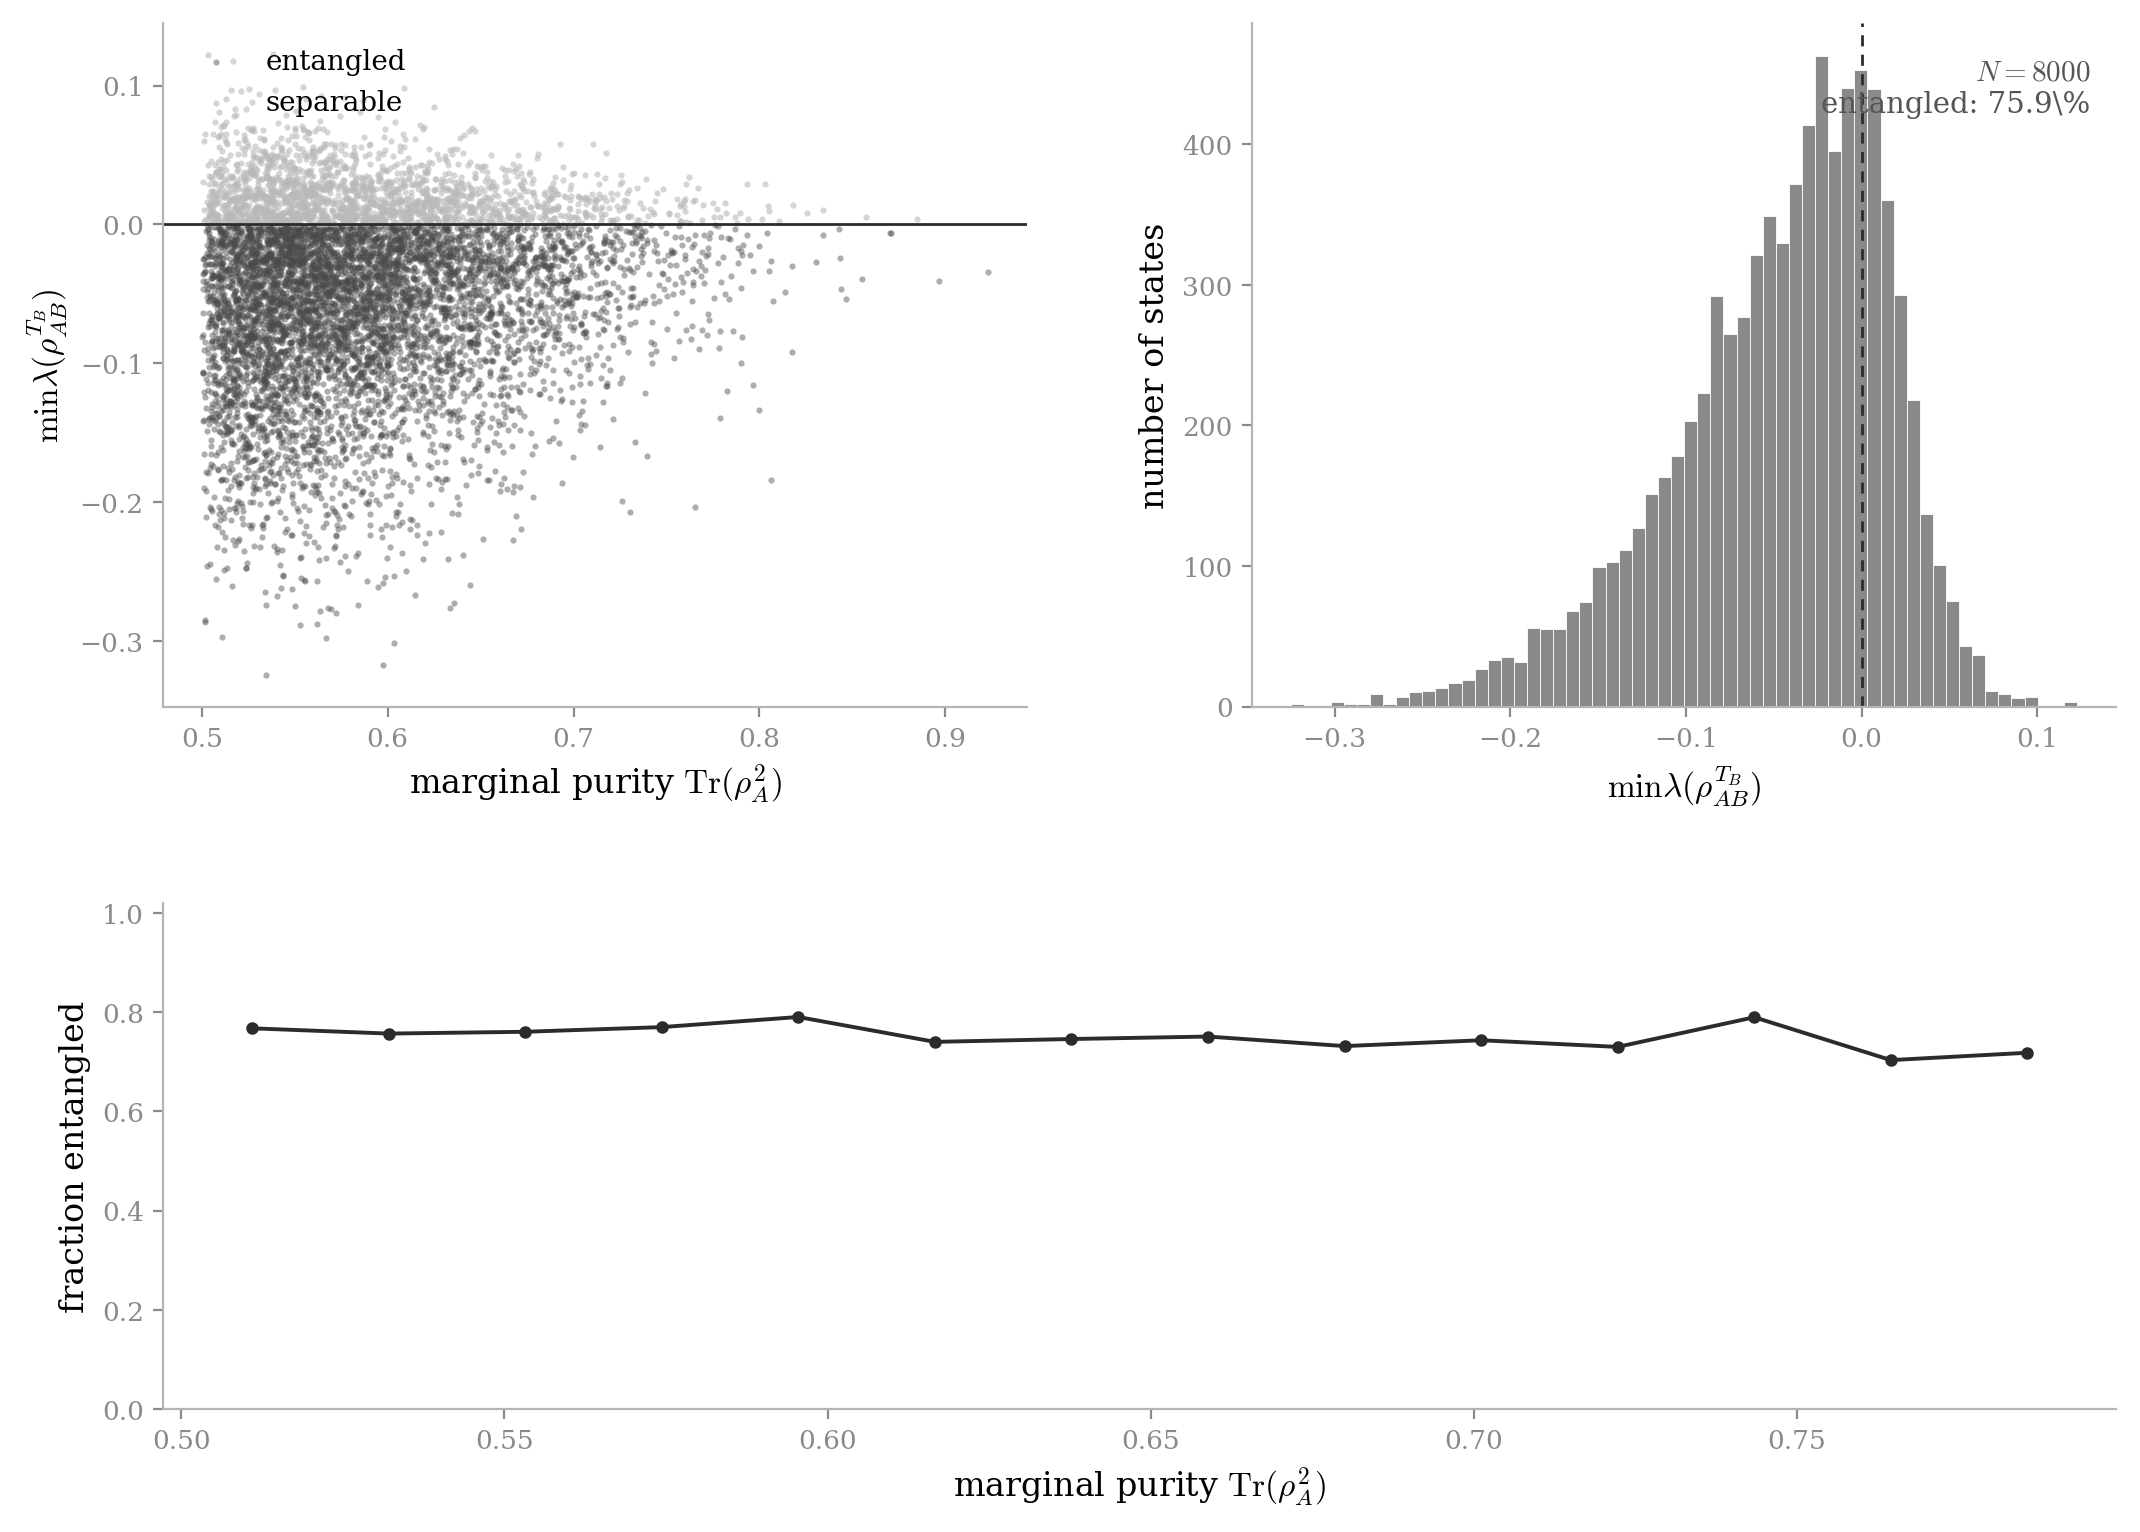
\includegraphics[width=0.95\linewidth]
{fig_toy_twoqubit_ppt_simulation_panel.png}
\captionsetup{justification=raggedright,singlelinecheck=false}
\caption{\textbf{Simulation witness for the two-qubit joint
admissibility toy.} Left: PPT witness value
\[
\min\lambda(\rho_{AB}^{T_B})
\]
versus marginal purity
\[
\mathrm{Tr}(\rho_A^2).
\]
Values below zero indicate entanglement, which is exact as a criterion
in \(2\times2\) systems. Entangled and separable points can coexist at
the same marginal purity, confirming that marginal purity does not
determine joint structure. Right: histogram of PPT witness values over
the Monte Carlo sample. Bottom: binned fraction of entangled states as a
function of marginal purity, showing no marginal-purity threshold that
recovers separability.}
\label{fig:toy_twoqubit_ppt_simulation_panel}
\end{figure}

\subsubsection{SSAF Structural Reading}
\label{toy:two_qubit_SSAF_structural_reading}

\paragraph{Structural reading.}

The toy states only that \(E\) can specify a jointly admissible sector
\[
\mathcal A_{AB}(E)
\]
containing non-separable configurations. In SSAF terms,
``entanglement'' labels non-factorizable joint admissibility under
fixed \(E\). No claim is made that one subsystem influences the other.
Correlations are constraints inherent to the jointly admissible sector.

\paragraph{The key implication that does not hold.}

Even when the marginal descriptions are admissible,
\[
\text{``admissible marginal descriptions''}
\;\not\Rightarrow\;
\text{``separable joint description.''}
\]

Nor does marginal admissibility determine joint admissibility. The
explanatory burden is placed on the structure of
\[
\mathcal A_{AB}(E)
\]
and its joint constraints, not on a dynamical signal mechanism.

\paragraph{Summary.}

A Bell state is non-separable while both marginals are maximally mixed.
In SSAF language this is the structural content: non-separable joint
admissibility under fixed \(E\). The correlations are read as
constraints inherent to the jointly admissible sector, not as
influences, not as signals, and not as evidence of any mechanism beyond
the joint constraint structure.

\subsubsection{General Form: Entanglement as Non-Separable Joint Admissibility}
\label{toy:entanglement_nonfactorizable}

\paragraph{General pass condition.}

The Bell-state construction above demonstrates the pass condition in a
concrete instance. Its general form names the set of all joint
configurations whose marginals are admissible,
\begin{equation}
\mathcal J(E)
:=
\bigl\{
\omega_{AB}\in\Phi_{AB}:
\mathrm{Tr}_B(\omega_{AB})\in\mathcal A_A(E),\;
\mathrm{Tr}_A(\omega_{AB})\in\mathcal A_B(E)
\bigr\},
\label{eq:toy_ent_JE}
\end{equation}
and requires that it be consistent for
\begin{equation}
\mathcal A_{AB}(E)\subsetneq\mathcal J(E),
\label{eq:toy_ent_strict_inclusion}
\end{equation}
with \(\mathcal A_{AB}(E)\) containing non-separable configurations
even when the corresponding marginals lie in
\[
\mathcal A_A(E),
\qquad
\mathcal A_B(E).
\]
That strict inclusion is what ``joint admissibility is not
reconstructible from marginals alone'' means formally.

The excluded interpretations established for the construction above
continue to apply. One exclusion is worth stating separately:
entanglement never enlarges access. It is a structural property of
joint admissibility, invariant under reconstruction relabeling
(Proposition~\ref{prop:nonfact_reconstruction_invariant}), and grants
no addressability outside the realized admissible domain.

\paragraph{Setup.}

Fix a factorization
\[
\mathcal H=\mathcal H_A\otimes\mathcal H_B
\]
and define
\[
\Phi_{AB}
:=
\mathcal D(\mathcal H_A\otimes\mathcal H_B),
\qquad
\Phi_A
:=
\mathcal D(\mathcal H_A),
\qquad
\Phi_B
:=
\mathcal D(\mathcal H_B).
\]

Fix classical context \(E\). The joint admissible set is
\begin{equation}
\mathcal A_{AB}(E)\subseteq\Phi_{AB},
\label{eq:toy_ent_joint_set}
\end{equation}
with induced marginal admissible sets
\begin{equation}
\mathcal A_A(E)
:=
\{
\mathrm{Tr}_B(\rho_{AB}):
\rho_{AB}\in\mathcal A_{AB}(E)
\},
\qquad
\mathcal A_B(E)
:=
\{
\mathrm{Tr}_A(\rho_{AB}):
\rho_{AB}\in\mathcal A_{AB}(E)
\}.
\label{eq:toy_ent_marginals}
\end{equation}

A joint configuration is \emph{separable} if it is a convex mixture of
product states; otherwise it is non-separable, or entangled
\cite{Horodecki2009,Watrous2018}.

\paragraph{Structural reading.}

Entanglement in this toy is the existence of a jointly admissible
configuration that is non-separable:
\[
\exists\,\rho_{AB}\in\mathcal A_{AB}(E)
\quad
\text{such that}
\quad
\rho_{AB}
\text{ is non-separable.}
\]

This is a statement about which joint configurations are admitted under
fixed \(E\), not about how outcomes occur or how states evolve.

\begin{lemma}[Marginals do not determine the joint state]
\label{lem:toy_ent_marginals_nondet}
There exist distinct
\[
\rho_{AB}\neq\sigma_{AB}\in\Phi_{AB}
\]
such that
\begin{equation}
\mathrm{Tr}_A(\rho_{AB})
=
\mathrm{Tr}_A(\sigma_{AB}),
\qquad
\mathrm{Tr}_B(\rho_{AB})
=
\mathrm{Tr}_B(\sigma_{AB}).
\label{eq:toy_ent_equal_marginals}
\end{equation}

Consequently, marginal data alone do not determine the joint
configuration.
\end{lemma}

\begin{proof}
Take
\[
\mathcal H_A\cong\mathcal H_B\cong\mathbb C^2.
\]
Let
\[
|\Phi^+\rangle
:=
\frac{|00\rangle+|11\rangle}{\sqrt2}
\]
and define
\[
\rho_{AB}
:=
|\Phi^+\rangle\langle\Phi^+|,
\qquad
\sigma_{AB}
:=
\frac14 I_{AB}.
\]

Then
\[
\rho_{AB}\neq\sigma_{AB},
\]
since one is pure and entangled while the other is maximally mixed and
separable. Yet
\[
\mathrm{Tr}_B(\rho_{AB})
=
\frac12 I_A
=
\mathrm{Tr}_B(\sigma_{AB}),
\qquad
\mathrm{Tr}_A(\rho_{AB})
=
\frac12 I_B
=
\mathrm{Tr}_A(\sigma_{AB}).
\]

Therefore the same pair of marginal states is compatible with distinct
joint configurations. Marginal data alone do not determine the joint
state.
\end{proof}

\begin{figure}[t]
\centering
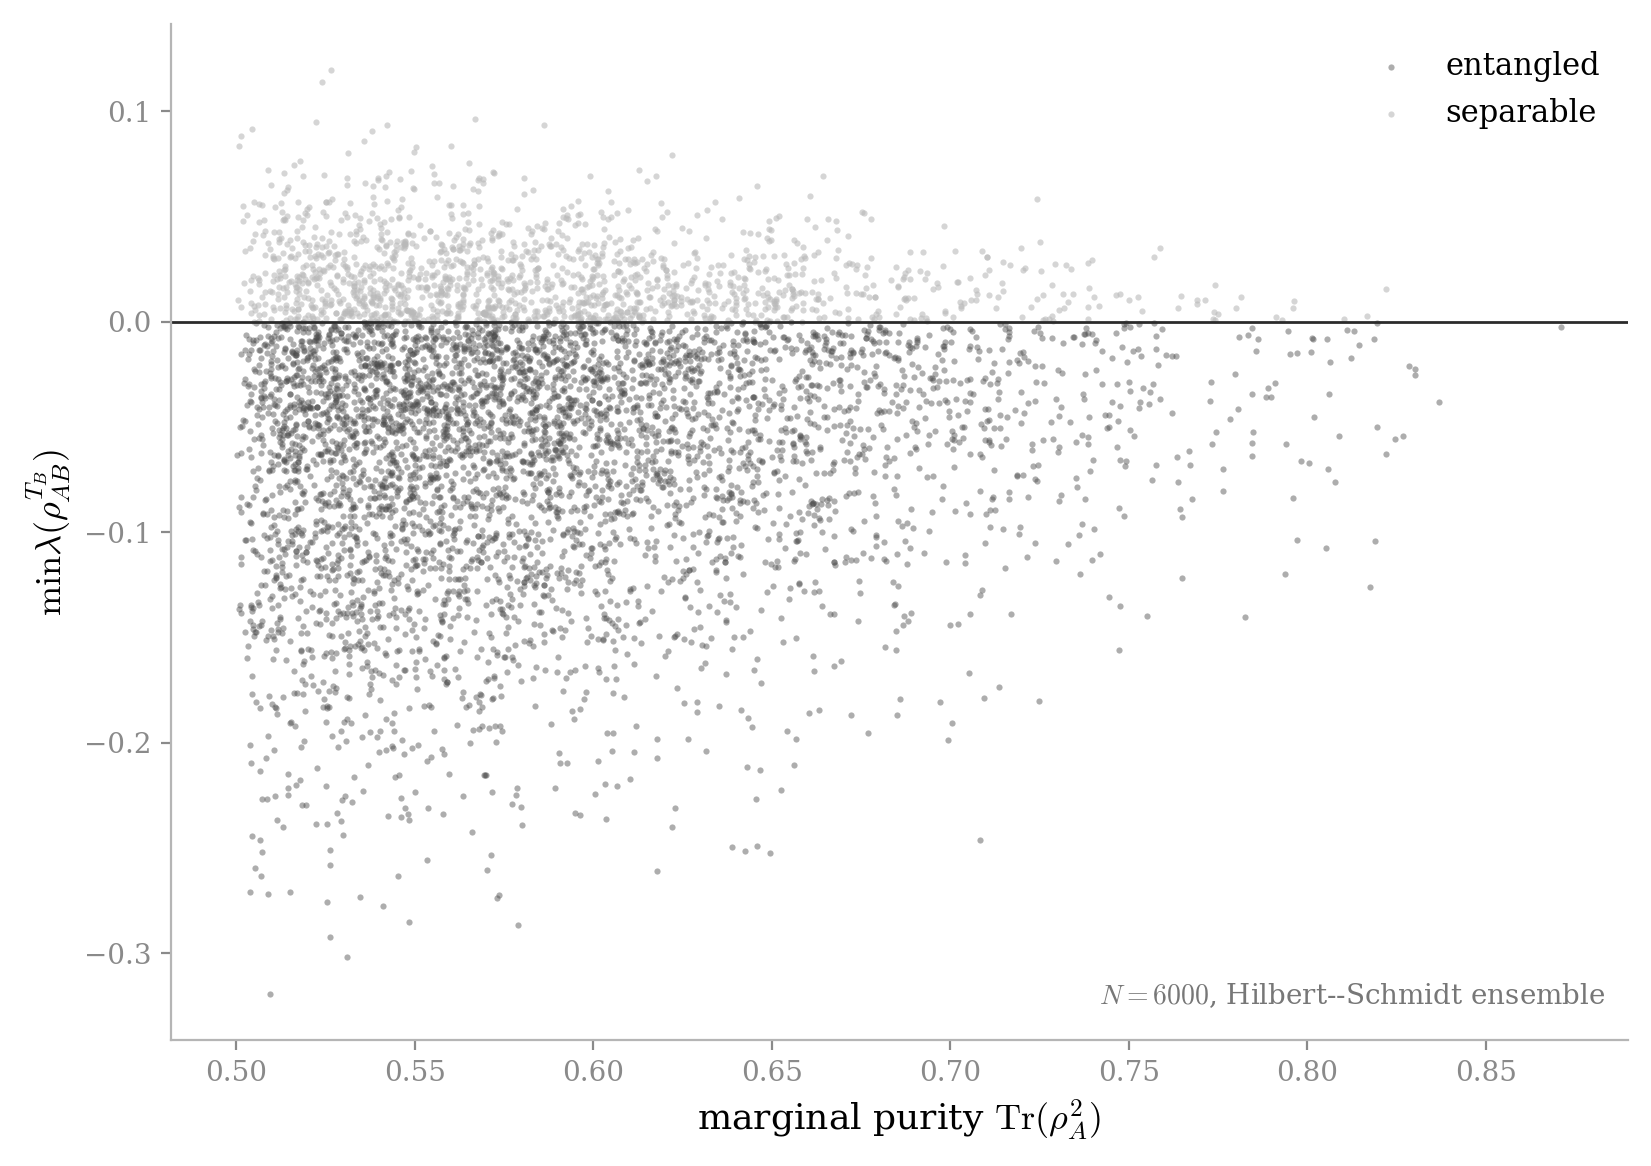
\includegraphics[width=0.82\linewidth]
{fig_toy_entanglement_ppt_vs_marginal_purity.png}
\captionsetup{justification=raggedright,singlelinecheck=false}
\caption{\textbf{Monte Carlo witness for the entanglement toy.}
Two-qubit joint configurations plotted by marginal purity
\[
\mathrm{Tr}(\rho_A^2)
\]
versus minimum eigenvalue of the partial transpose
\[
\min\lambda(\rho_{AB}^{T_B}).
\]
Values below zero certify entanglement; the PPT criterion is necessary
and sufficient in \(2\times2\). Entangled and separable states can
coexist at the same marginal purity, confirming that marginal purity
does not determine joint structure.}
\label{fig:toy_entanglement_ppt_vs_marginal_purity}
\end{figure}

\begin{corollary}[Joint admissibility can be strictly stronger than marginal admissibility]
\label{cor:toy_ent_strict}
It is consistent for
\[
\mathcal A_{AB}(E)\subsetneq\mathcal J(E).
\]
That is, even if a joint configuration \(\omega_{AB}\) has marginals in
\[
\mathcal A_A(E)
\qquad
\text{and}
\qquad
\mathcal A_B(E),
\]
it need not be jointly admissible.
\end{corollary}

\begin{proof}
Let
\[
\rho_{AB}
=
|\Phi^+\rangle\langle\Phi^+|
\]
and
\[
\sigma_{AB}
=
\frac14 I_{AB}
\]
as in Lemma~\ref{lem:toy_ent_marginals_nondet}. Define a toy joint
admissible sector
\[
\mathcal A_{AB}(E)
:=
\{\rho_{AB}\}.
\]

Then the induced marginal admissible sets are
\[
\mathcal A_A(E)=\left\{\frac12 I_A\right\},
\qquad
\mathcal A_B(E)=\left\{\frac12 I_B\right\}.
\]

By definition,
\[
\sigma_{AB}\in\mathcal J(E),
\]
because its marginals lie in the induced marginal admissible sets.
However,
\[
\sigma_{AB}\notin\mathcal A_{AB}(E).
\]

Therefore
\[
\mathcal A_{AB}(E)\subsetneq\mathcal J(E).
\]
This proves consistency of strict inclusion.
\end{proof}

\paragraph{Compatibility with NS1 and CPTP updating.}

All admissible updating maps remain linear CPTP with parameters
depending only on \(E\). Non-separability of an admissible joint state
is an operator property of an element of
\[
\mathcal A_{AB}(E).
\]

It introduces no state-dependent parameters, outcome selection,
nonlinear evolution, signalling mechanism, or retro-admissibility.

The toy also does not retune
\[
\Gamma_E,
\qquad
\mathcal N_E,
\qquad
\mu_E.
\]

\paragraph{Relation to other toys.}

This toy operates entirely within a fixed joint admissible sector. It
does not alter envelope structure, does not enable cross-envelope
addressability, and does not introduce sequencing.

Envelope non-closure and sequencing toys concern admissible domains,
map domains, and addressability restriction. This toy concerns the
internal structure of the jointly admissible set.

\subsection{Toy Model: Coherence Basin via a Scalar Depth Functional}
\label{toy:coherence_basin_depth_functional_contraction}

\noindent\emph{Axiom target:} Axioms~III and VIII (Coherence Diagnostics; Basin Organization).

\paragraph{Axiom unit test: pass condition.}

The framework must admit a basin-style template in
\[
\Phi=\mathcal D(\mathcal H)
\]
defined purely by:

\begin{enumerate}[label=(\roman*), leftmargin=2.2em]
\item a scalar distance-to-core diagnostic for a context-indexed core
set; and
\item NS1-safe updating, i.e.\ linear CPTP maps whose parameters depend
only on \(E\).
\end{enumerate}

The template must show monotone approach toward the declared core under
iteration without requiring spacetime ontology, force laws, curvature
claims, outcome targeting, state-conditioned retuning, or additional
dynamics.

Any irreversibility must arise from ordinary CPTP contractivity and
failure of CPTP recoverability, with exact non-invertibility appearing
only in projected, coarse-grained, or asymptotic limits.

\paragraph{What this toy shows.}

The ``coherence basin'' language used throughout SSAF admits a concrete
structural template. A scalar diagnostic measuring distance to a
distinguished core set, combined with an NS1-safe CPTP channel family,
can produce monotone approach toward the core along a bookkeeping chain.

The irreversibility is not a new physical law. It is the standard
operator-theoretic fact that CPTP maps contract distinguishability and
that the inverse of a dissipative channel, when it exists as a linear
map, is generally not CPTP.

The gravity correspondence, basin descent as the structural analogue of
descent along a scalar potential, is mathematical and representational,
not ontological.

\paragraph{Setup.}

Fix a classical context \(E\) determining:

\begin{itemize}

\item a distinguished \emph{core set}
\[
\mathcal M(E)\subseteq\Phi,
\]
the basin floor; and

\item an admissible updating family
\[
\{\Lambda_{E,\Delta}\}_{\Delta\geq 0}
\]
of linear CPTP maps whose parameters depend only on \(E\), in
accordance with NS1.

\end{itemize}

No object in this toy is selected as a function of \(\rho\), outcomes,
ensemble decompositions, or state-derived diagnostics. The toy also
does not retune
\[
\Gamma_E,
\qquad
\mathcal N_E,
\qquad
\mu_E.
\]

\subsubsection{Distance-to-Core Functional}
\label{toy:basin_depth_functional}

\paragraph{Definition.}

Fix a CPTP-contractive distinguishability metric \(d(\cdot,\cdot)\) on
states, for example trace distance
\[
d(\rho,\sigma)
:=
\frac12\|\rho-\sigma\|_1.
\]

Define the scalar distance-to-core functional
\begin{equation}
D_E(\rho)
:=
\inf_{\sigma\in\mathcal M(E)}
d(\rho,\sigma).
\label{eq:basin_depth_def}
\end{equation}

Small \(D_E(\rho)\) means the configuration is close to the declared
core. Large \(D_E(\rho)\) means it lies farther from the core in the
chosen diagnostic geometry.

The term ``basin depth'' is therefore conventional: in this toy,
monotone basin descent corresponds to non-increase of
\(D_E\), i.e.\ decreasing distance to the core.

\paragraph{Core-set invariance.}

Assume the core set is invariant under admissible updating:
\begin{equation}
\Lambda_{E,\Delta}(\mathcal M(E))
\subseteq
\mathcal M(E)
\qquad
\text{for all }\Delta\geq 0.
\label{eq:core_invariance}
\end{equation}

This expresses that \(\mathcal M(E)\) is a stable sector under the
declared \(E\)-indexed admissible maps. It is a structural assumption
about the toy, not a force law, attractor dynamics, or physical
potential.

\begin{lemma}[Distance-to-core is non-increasing under invariant-core CPTP maps]
\label{lem:depth_nonexpansion}
Let \(d\) be CPTP-contractive and define \(D_E\) by
Eq.~\eqref{eq:basin_depth_def}. If Eq.~\eqref{eq:core_invariance}
holds, then for all \(\rho\in\Phi\) and all \(\Delta\geq 0\),
\begin{equation}
D_E\!\bigl(\Lambda_{E,\Delta}(\rho)\bigr)
\leq
D_E(\rho).
\label{eq:basin_nonexpansion}
\end{equation}
\end{lemma}

\begin{proof}
For any
\[
\sigma\in\mathcal M(E),
\]
CPTP contractivity gives
\[
d\bigl(
\Lambda_{E,\Delta}(\rho),
\Lambda_{E,\Delta}(\sigma)
\bigr)
\leq
d(\rho,\sigma).
\]

By core-set invariance,
\[
\Lambda_{E,\Delta}(\sigma)\in\mathcal M(E).
\]
Therefore
\[
D_E(\Lambda_{E,\Delta}(\rho))
=
\inf_{\tau\in\mathcal M(E)}
d(\Lambda_{E,\Delta}(\rho),\tau)
\leq
d\bigl(
\Lambda_{E,\Delta}(\rho),
\Lambda_{E,\Delta}(\sigma)
\bigr)
\leq
d(\rho,\sigma).
\]

Taking the infimum over
\[
\sigma\in\mathcal M(E)
\]
yields the claim.
\end{proof}

\subsubsection{Monotone Descent and Strict Contraction}
\label{toy:basin_monotone_descent}

\paragraph{Monotone basin descent.}

Lemma~\ref{lem:depth_nonexpansion} implies that admissible updating
under fixed \(E\) never increases the distance-to-core diagnostic:
\[
D_E(\Lambda_{E,\Delta}(\rho))
\leq
D_E(\rho).
\]

This defines a basin-style restriction ordering along a bookkeeping
index, without introducing a dynamical law, force, potential, or
fundamental clock.

\paragraph{Optional strict contraction.}

On declared subsets of \(\Phi\), for example after excluding fixed-point
sectors, one may have
\begin{equation}
D_E\!\bigl(\Lambda_{E,\Delta}(\rho)\bigr)
\leq
\lambda(E,\Delta)\,D_E(\rho)
\qquad
\text{for all }\rho\in\mathcal S(E)\subseteq\Phi,
\label{eq:basin_strict_contraction}
\end{equation}
with
\[
\lambda(E,\Delta)\in[0,1).
\]

This is an additional toy assumption, not a consequence of CPTP
contractivity alone. When it holds, the basin exhibits exponential
convergence toward the core on \(\mathcal S(E)\).

\paragraph{Sequencing chain.}

Choose nonnegative labels
\[
\{\Delta_n\}_{n\geq 1}
\]
and define
\[
\rho_{n+1}
:=
\Lambda_{E,\Delta_{n+1}}(\rho_n).
\]

By iterating Eq.~\eqref{eq:basin_nonexpansion},
\[
D_E(\rho_{n+1})
\leq
D_E(\rho_n).
\]

If Eq.~\eqref{eq:basin_strict_contraction} holds uniformly on
\(\mathcal S(E)\), then
\begin{equation}
D_E(\rho_n)
\leq
\Bigl(
\prod_{j=1}^n
\lambda(E,\Delta_j)
\Bigr)
D_E(\rho_0),
\qquad
\rho_0\in\mathcal S(E).
\label{eq:basin_iterated_descent}
\end{equation}

All map parameters and contraction factors depend only on \(E\) and
externally specified labels \(\Delta_j\). No state-conditioned
selection is introduced.

\subsubsection{Concrete Instantiation: Amplitude Damping}
\label{toy:basin_concrete_instantiation}

\paragraph{Single-qubit example.}

Let
\[
\mathcal H=\mathbb C^2
\]
and choose the core
\[
\mathcal M(E)
=
\{|0\rangle\langle0|\}.
\]

Let \(\Lambda_{E,\eta}\) be the standard amplitude-damping channel with
\[
\eta=\eta(E)\in[0,1]
\]
fixed by \(E\):
\[
\Lambda_{E,\eta}(\rho)
=
K_0\rho K_0^\dagger
+
K_1\rho K_1^\dagger,
\]
where
\[
K_0
=
\begin{pmatrix}
1 & 0\\
0 & \sqrt{1-\eta}
\end{pmatrix},
\qquad
K_1
=
\begin{pmatrix}
0 & \sqrt{\eta}\\
0 & 0
\end{pmatrix}.
\]

With trace distance and core \(|0\rangle\langle0|\),
\begin{equation}
D_E(\rho)
=
\frac12
\bigl\|
\rho-|0\rangle\langle0|
\bigr\|_1.
\label{eq:basin_depth_trace_qubit}
\end{equation}

Writing
\[
\rho
=
\begin{pmatrix}
\rho_{00} & \rho_{01}\\
\rho_{10} & \rho_{11}
\end{pmatrix},
\]
a direct calculation gives
\begin{equation}
D_E(\rho)
=
\sqrt{\rho_{11}^2+|\rho_{01}|^2},
\qquad
D_E(\Lambda_{E,\eta}(\rho))
=
\sqrt{
(1-\eta)^2\rho_{11}^2
+
(1-\eta)|\rho_{01}|^2
}.
\label{eq:basin_depth_qubit_closed_form}
\end{equation}

Hence
\begin{equation}
D_E(\Lambda_{E,\eta}(\rho))
\leq
\sqrt{1-\eta}\;D_E(\rho).
\label{eq:basin_strict_contraction_qubit}
\end{equation}

For
\[
0<\eta\leq 1,
\]
the contraction factor
\[
\lambda(E)=\sqrt{1-\eta(E)}
\]
lies in \([0,1)\). For \(\eta=0\), the channel is the identity and
\(D_E\) is unchanged.

\paragraph{What this means.}

The amplitude-damping channel drives every qubit state toward
\[
|0\rangle\langle0|
\]
under repeated application when \(0<\eta(E)\leq 1\). It contracts both
the excited-state population \(\rho_{11}\) and the off-diagonal
coherence \(\rho_{01}\).

The bound Eq.~\eqref{eq:basin_strict_contraction_qubit} gives uniform
exponential contraction in the number of steps whenever
\[
0<\eta(E)\leq 1.
\]

For \(0<\eta<1\), the channel is generally linearly invertible on the
operator space, but its inverse is not CPTP and therefore is not an
admissible recovery operation. For \(\eta=1\), the channel is genuinely
non-injective and maps all input states to the core state.

Thus this is a concrete CPTP realization of basin-style descent with no
forces, no spacetime geometry, no state-conditioned tuning, and no
retro-admissibility channel.

\subsubsection{Structural Correspondence: Basin as Gravity Analog}
\label{toy:basin_gravity_analogy_justification}

\paragraph{Structural correspondence only.}

Classical gravity is often represented, in the Newtonian limit, as
motion relative to a scalar potential. This toy uses that familiar
structural template inside \(\Phi\) without identifying the two domains:

\begin{itemize}
\item scalar diagnostic: \(D_E(\rho)\);
\item contracted set or basin floor: \(\mathcal M(E)\);
\item contraction rule: \(\rho\mapsto\Lambda_{E,\Delta}(\rho)\);
\item irreversibility: CPTP contractivity and failure of admissible
CPTP recovery.
\end{itemize}

The correspondence is mathematical and diagnostic, not ontological.
No claim is made that gravity is a CPTP channel, that spacetime
curvature is coherence depth, or that SSAF derives gravitational
dynamics here.

\paragraph{Constraint from large-scale inverse-square behavior.}

Recent cosmological-scale tests indicate that gravitational attraction
continues to weaken approximately according to inverse-square scaling
across galaxy-cluster separations extending tens to hundreds of
megaparsecs~\cite{Gallardo2026GravityForceLaw}. Within SSAF, this does
not elevate gravity, metric distance, curvature, or spacetime geometry
to primitive status.

Instead, it constrains any admissible reconstruction of effective
geometry: any emergent space-like representation licensed by
admissibility, compatibility, addressability, sequencing, and declared
structural organization must reproduce the observed large-scale
inverse-square phenomenology to high accuracy.

Accordingly, SSAF treats inverse-square scaling not as a foundational
axiom but as a reconstruction constraint on any effective geometric
description compatible with observation.

\paragraph{Structural takeaway.}

A scalar distance-to-core functional together with NS1-safe CPTP
contraction suffices to generate a basin-style template with
irreversible restriction in configuration space. This provides the
structural backbone for coherence-basin language throughout the paper
and justifies the gravity correspondence strictly as a basin-descent
analogy.

It introduces no primitive force, metric, background time, spacetime
ontology, or gravitational dynamics.

\subsection{Toy Model: Envelope-Bound Resolution and Non-Addressability of Incompatible Ordering Classes}
\label{toy:envelope_bound_resolution_stronger}

\noindent\emph{Axiom target:} Axiom~VII (NS1) and envelope-local updating discipline.

\paragraph{Axiom unit test: pass condition.}

The framework must admit envelope-local admissible updating such that,
under fixed classical context \(E\), in accordance with NS1:

\begin{enumerate}[label=(\roman*), leftmargin=2.2em]
\item the admissible map family is closed on a declared envelope-domain;
\item any ``cross-envelope reconfiguration'' is \emph{undefined}
relative to that admissibility structure, not a suppressed process.
\end{enumerate}

The pass condition is structural: closure and non-addressability must
follow from domain and codomain invariance of an \(E\)-indexed CPTP
class,
without adding spacetime primitives, outcome-conditioned rules, or
state-dependent tuning.

\paragraph{What this toy shows.}

The ancestor-elimination thought experiment
(Appendix~C, Sec.~\ref{appC:toy_ancestor_elimination}) established that
cross-envelope access is structurally undefined in SSAF. This toy
provides a finite-dimensional witness for that claim: a concrete CPTP
channel family that is closed on each declared envelope, so any map
crossing envelope boundaries is absent from the admissible class.

The unavailability is not a prohibition. It is a domain/codomain
closure statement.

\paragraph{Scope.}

This toy concerns domain-of-definition only. An envelope decomposition
and an admissible CPTP class are assumed, and envelope invariance within
that class is shown. The toy does not explain the origin of envelopes,
does not analyze extensions that add cross-envelope maps, and does not
claim that all CPTP maps preserve the envelopes.

\paragraph{Setup.}

Let \(\mathcal H\) be finite-dimensional and
\[
\Phi:=\mathcal D(\mathcal H).
\]
Fix a classical context \(E\) and admissible sector
\[
\mathcal A(E)\subseteq\Phi.
\]

Assume a disjoint partition into declared envelope domains:
\begin{equation}
\mathcal A(E)
=
\bigsqcup_{i\in I}\mathcal E_i(E),
\qquad
\mathcal E_i(E)\cap\mathcal E_j(E)=\varnothing
\quad
(i\neq j).
\label{eq:env_partition_strong}
\end{equation}

A realized interface acts on one envelope
\[
\mathcal E_\star(E).
\]
States in other \(\mathcal E_j(E)\) are non-addressable within that
realized description.

These envelopes are toy-domain structures. They are not assumed to be
topological connected components, metric regions, \(\Gamma_E\)
components, \(\mathcal N_E\)-neighbourhoods, or \(\mu_E\)-measured
regions unless a model-specific construction explicitly says so.

\subsubsection{Finite Witness: Direct-Sum Sectors and Envelope-Invariant CPTP Maps}
\label{subsubsec:env_witness_strong}

\paragraph{Direct-sum decomposition.}

Let
\[
\mathcal H=\mathcal H_0\oplus\mathcal H_1
\]
with orthogonal projectors \(P_0,P_1\) satisfying
\[
P_0+P_1=\mathbf 1.
\]

Define two disjoint envelopes as faces supported on each sector:
\begin{equation}
\mathcal E_i(E)
:=
\bigl\{
\rho\in\mathcal D(\mathcal H):
\rho=P_i\rho P_i,\;
\mathrm{Tr}(P_i\rho)=1
\bigr\},
\qquad
i\in\{0,1\}.
\label{eq:env_faces_strong}
\end{equation}

Set
\[
\mathcal A(E):=\mathcal E_0(E)\sqcup\mathcal E_1(E).
\]

Thus \(\mathcal E_0(E)\) consists of all density operators supported
entirely on \(\mathcal H_0\), and \(\mathcal E_1(E)\) consists of all
density operators supported entirely on \(\mathcal H_1\). They share no
elements.

\paragraph{Admissible map family.}

Define the admissible channel class under \(E\) to consist of CPTP maps
admitting a Kraus representation with block-diagonal Kraus operators:
\begin{equation}
\mathcal T^E(\rho)
=
\sum_k K_k\rho K_k^\dagger,
\qquad
\sum_k K_k^\dagger K_k=\mathbf 1,
\qquad
K_k=P_0K_kP_0+P_1K_kP_1
\quad
\forall k.
\label{eq:block_diag_kraus_strong}
\end{equation}

Block-diagonal here means each Kraus operator preserves the direct-sum
sectors. It acts within \(\mathcal H_0\) and within \(\mathcal H_1\),
with no terms mapping between the two sectors.

This is a declared admissible subclass of CPTP maps, not a claim about
all CPTP maps.

\begin{lemma}[Block-diagonal Kraus operators preserve envelopes]
\label{lem:block_diag_preserves_env}
If \(\mathcal T^E\) admits a Kraus representation satisfying
Eq.~\eqref{eq:block_diag_kraus_strong}, then each envelope
\(\mathcal E_i(E)\) is invariant. That is, for
\[
\rho\in\mathcal E_i(E),
\]
one has
\[
\mathcal T^E(\rho)\in\mathcal E_i(E).
\]
\end{lemma}

\begin{proof}
Fix \(i\in\{0,1\}\) and let
\[
\rho\in\mathcal E_i(E),
\]
so
\[
\rho=P_i\rho P_i.
\]

Block-diagonality implies
\[
P_{1-i}K_kP_i=0
\]
for all \(k\). Hence
\[
P_{1-i}\mathcal T^E(\rho)P_{1-i}
=
\sum_k
(P_{1-i}K_kP_i)\rho(P_{1-i}K_kP_i)^\dagger
=
0.
\]

Therefore \(\mathcal T^E(\rho)\) has no support on
\(\mathcal H_{1-i}\), so
\[
\mathcal T^E(\rho)
=
P_i\mathcal T^E(\rho)P_i.
\]

Trace preservation gives
\[
\mathrm{Tr}(\mathcal T^E(\rho))=1,
\]
and since the output is supported on \(\mathcal H_i\),
\[
\mathrm{Tr}(P_i\mathcal T^E(\rho))=1.
\]

Thus
\[
\mathcal T^E(\rho)\in\mathcal E_i(E).
\]
\end{proof}

\begin{corollary}[No cross-envelope map within the admissible family]
\label{cor:no_cross_env_in_family}
Within the channel class Eq.~\eqref{eq:block_diag_kraus_strong}, there
is no CPTP map \(\mathcal T^E\) and no
\[
\rho\in\mathcal E_0(E)
\]
such that
\[
\mathcal T^E(\rho)\in\mathcal E_1(E),
\]
and likewise with \(0\) and \(1\) interchanged.

Any CPTP map that transfers support from \(\mathcal H_0\) to
\(\mathcal H_1\) requires cross-block action and therefore lies outside
the declared admissible family.
\end{corollary}

\subsubsection{Envelope-Local Updating Under NS1}
\label{subsubsec:resolution_sequencing_env_local_strong}

Under NS1, admissible updating is represented by linear CPTP maps whose
parameters depend only on fixed \(E\), never on \(\rho\), outcomes,
ensemble decompositions, or state-derived diagnostics
\cite{Kraus1983,Lindblad1976,Gorini1976,Watrous2018,Wilde2017}.

Represent an \(E\)-indexed admissible family
\[
\{\mathcal T^E_\Delta\}_{\Delta\geq 0}
\]
whose operationally licensed use is envelope-local:
\begin{equation}
\mathcal T^E_\Delta:
\mathcal E_\star(E)
\longrightarrow
\mathcal E_\star(E).
\label{eq:env_local_family_strong}
\end{equation}

More precisely, \(\mathcal T^E_\Delta\) is a CPTP map on \(\Phi\), but
the declared admissible domain and codomain for the realized
description are both \(\mathcal E_\star(E)\).

Iterating along any bookkeeping index yields a closed chain
\[
\rho_{n+1}
=
\mathcal T^E_{\Delta_{n+1}}(\rho_n),
\]
with
\[
\rho_n\in\mathcal E_\star(E)
\]
for all \(n\).

\subsubsection{Cross-Envelope Reconfiguration is Undefined}
\label{subsubsec:cross_env_undefined_stronger}

Let
\[
\rho_{\mathrm{target}}\in\mathcal E_j(E),
\qquad
j\neq\star.
\]

Reaching it from within the realized envelope would require a licensed
map of the form
\begin{equation}
\mathcal T:
\mathcal E_\star(E)
\longrightarrow
\mathcal E_j(E),
\qquad
j\neq\star.
\label{eq:cross_env_map_strong}
\end{equation}

No such map exists in the declared admissible class
Eq.~\eqref{eq:block_diag_kraus_strong}. Cross-envelope reconfiguration
is therefore not prohibited by a dynamical law. It is absent from the
defined domain/codomain structure of the witness model.

\paragraph{Structural takeaway.}

Existence of other envelopes in \(\Phi\) does not imply addressability
under a fixed \(E\)-indexed admissible map family. Another envelope can
coexist in \(\Phi\) while remaining inaccessible from within the
realized description: not hidden, not suppressed, simply outside the
licensed domain.

\subsubsection{Paradox Patterns Fail by Non-Addressability}
\label{subsubsec:paradox_fail_by_nonaddressability_strong}

Closed-loop paradox constructions require extending addressability
across incompatible ordering classes. In this witness, the realized
ordering is the closed envelope-domain
\[
\mathcal E_\star(E)
\]
under envelope-invariant admissible updating.

Any attempted intervention targeting
\[
\mathcal E_j(E),
\qquad
j\neq\star,
\]
requires a map of the form Eq.~\eqref{eq:cross_env_map_strong}, which is
not defined in the admissible structure.

This is the formal content behind the thought experiment in
Appendix~C: the ancestor-elimination scenario fails not because it is
dynamically forbidden, but because the map required to implement it is
not in the admissible class. There is nothing to forbid. There is
simply no such map within the declared fixed-\(E\) admissible class.

\paragraph{Witness recap.}

The toy uses
\[
\mathcal H=\mathcal H_0\oplus\mathcal H_1
\]
with envelopes Eq.~\eqref{eq:env_faces_strong} and admissible channels
restricted to block-diagonal Kraus families
Eq.~\eqref{eq:block_diag_kraus_strong}.

Lemma~\ref{lem:block_diag_preserves_env} gives envelope invariance.
Corollary~\ref{cor:no_cross_env_in_family} gives the absence of
cross-envelope maps.

Under NS1, this is a domain/codomain closure statement with no
state-conditioned or outcome-conditioned selection.

\subsection{Toy Model: Envelope-Bound Ordering on the Phase Circle}
\label{toy:envelope_ordering}

\noindent\emph{Axiom target:} Axiom~II (Phase as a Structural Descriptor).

\paragraph{Axiom unit test (pass condition).}
Under fixed classical context $E$ (NS1), membership in a phase-offset
acceptance window $W_E \subset S^1$ must be sufficient to (i) define
a directed participation predicate, and (ii) certify participation
failure purely as \emph{window non-closure}: for some pair $(i,j)$,
neither the offset $\Delta\phi_{ij}$ nor its antipode
$A(\Delta\phi_{ij})$ lies in the fixed window. Pass means: failure is
domain-of-definition (membership) only, no rates, dynamics, or
outcome-conditioned rules are introduced to ``fix'' it.

\paragraph{What this toy shows.}
Throughout SSAF, compatibility between configurations is described
using envelope constraints. This toy gives a concrete, calculable
instance of that idea using phase offsets on the circle $S^1$. Two
configurations either have a phase relationship that falls inside the
acceptance window (compatible, participation licensed) or they do not
(incompatible, participation undefined, not merely forbidden, but
outside the domain of the predicate). The regime map shows how the
set of licensed participations changes as the context $E$ changes the
window size, without any state-conditioned tuning.

\paragraph{What breaks it.}
The toy collapses if you allow any state- or outcome-conditioned
retuning of the window (e.g.\ choosing half-widths as a function of
observed offsets), or if you replace ``undefined by membership'' with
a hidden repair map that forces closure. Either move reintroduces an
illicit steering channel.

\paragraph{Scope.}
Finite structural witness in phase-offset space on $S^1$. Admissibility
is window membership. No dynamics, generators, rates, temporal
parameters, hidden variables, or outcome-conditioned rules.

\subsubsection{Primitive Data: Four Configurations on a Phase Circle}
\label{subsubsec:toy_phasecircle_data}

Let the configuration set be finite:
\begin{equation}
\mathcal{S} := \{\rho_1, \rho_2, \rho_3, \rho_4\}.
\label{eq:toy_phasecircle_states}
\end{equation}
Assign each configuration a phase descriptor on
$S^1 \cong \mathbb{R}/2\pi\mathbb{Z}$:
\begin{equation}
\phi(\rho_1) = 0, \quad
\phi(\rho_2) = \frac{\pi}{3}, \quad
\phi(\rho_3) = \pi, \quad
\phi(\rho_4) = \frac{4\pi}{3}.
\label{eq:toy_phasecircle_phases}
\end{equation}
Define directed offsets
\begin{equation}
\Delta\phi_{ij} :=
\bigl(\phi(\rho_j) - \phi(\rho_i)\bigr) \bmod 2\pi,
\label{eq:toy_phasecircle_offsets}
\end{equation}
and the principal-value representative
$\mathrm{PV} : S^1 \to (-\pi,\pi]$:
\begin{equation}
\Delta\phi_{ij}^{\mathrm{PV}} :=
\mathrm{PV}(\Delta\phi_{ij}) \in (-\pi,\pi].
\label{eq:toy_phasecircle_pv}
\end{equation}
Define the antipode $A : S^1 \to S^1$ by
\begin{equation}
A(\theta) := \theta + \pi \bmod 2\pi,
\qquad A \circ A = \mathrm{id}.
\label{eq:toy_phasecircle_antipode}
\end{equation}
For this phase assignment, the only distinct principal-value offsets
occurring for $i \neq j$ are
\begin{equation}
\mathcal{D} :=
\Bigl\{\pm\frac{\pi}{3},\; \pm\frac{2\pi}{3},\; \pi\Bigr\}.
\label{eq:toy_phasecircle_discrete_offsets}
\end{equation}

\subsubsection{Phase-Offset Acceptance Window}
\label{subsubsec:toy_phasecircle_window}

Let $\Delta_0(E) \in (0,\pi]$ be the half-width of the near-$0$
window and $\Delta_\pi(E) \in (0,\pi]$ the half-width of the
near-$\pi$ window. Define
\begin{equation}
\theta \in W_E(\Delta_0(E), \Delta_\pi(E))
\;\Longleftrightarrow\;
\bigl(|\mathrm{PV}(\theta)| \le \Delta_0(E)\bigr)
\;\text{or}\;
\bigl(|\mathrm{PV}(\theta)| \ge \pi - \Delta_\pi(E)\bigr).
\label{eq:toy_phasecircle_window_def}
\end{equation}
The window has two lobes: one centered at $0$ (near-in-phase) and one
centered at $\pi$ (near-antiphase). The half-widths $\Delta_0(E)$ and
$\Delta_\pi(E)$ depend only on the fixed classical context $E$, never
on $\rho$ or outcomes (NS1).

\subsubsection{Directed Participation as Window Membership}
\label{subsubsec:toy_phasecircle_ordering_predicate}

Define
\begin{equation}
\rho_i \triangleleft_E \rho_j
\;\Longleftrightarrow\;
\Delta\phi_{ij}^{\mathrm{PV}} \in
W_E(\Delta_0(E), \Delta_\pi(E)).
\label{eq:toy_phasecircle_ordering_relation}
\end{equation}
This is a membership predicate only; no order axioms are assumed.

\subsubsection{Worked Evaluation and Regime Changes}
\label{subsubsec:toy_phasecircle_worked_eval}

\paragraph{Instance: $\Delta_0(E) = \pi/2$, $\Delta_\pi(E) = \pi/6$.}
The principal-value offsets for $i \neq j$ are:
\begin{align}
\Delta\phi^{\mathrm{PV}}_{12} &= \tfrac{\pi}{3}, &
\Delta\phi^{\mathrm{PV}}_{13} &= \pi, &
\Delta\phi^{\mathrm{PV}}_{14} &= -\tfrac{2\pi}{3},\\
\Delta\phi^{\mathrm{PV}}_{21} &= -\tfrac{\pi}{3}, &
\Delta\phi^{\mathrm{PV}}_{23} &= \tfrac{2\pi}{3}, &
\Delta\phi^{\mathrm{PV}}_{24} &= \pi,\\
\Delta\phi^{\mathrm{PV}}_{31} &= \pi, &
\Delta\phi^{\mathrm{PV}}_{32} &= -\tfrac{2\pi}{3}, &
\Delta\phi^{\mathrm{PV}}_{34} &= \tfrac{\pi}{3},\\
\Delta\phi^{\mathrm{PV}}_{41} &= \tfrac{2\pi}{3}, &
\Delta\phi^{\mathrm{PV}}_{42} &= \pi, &
\Delta\phi^{\mathrm{PV}}_{43} &= -\tfrac{\pi}{3}.
\end{align}
The near-$0$ window includes $|\cdot| \le \pi/2$ (so $\pm\pi/3$ yes,
$\pm 2\pi/3$ no), and the near-$\pi$ window includes
$|\cdot| \ge 5\pi/6$ (so $\pi$ yes). The directed edges are:
\begin{equation}
(1 \leftrightarrow 2),\quad
(3 \leftrightarrow 4),\quad
(1 \leftrightarrow 3),\quad
(2 \leftrightarrow 4),
\label{eq:toy_phasecircle_admissible_edges_hot}
\end{equation}
and $(1 \leftrightarrow 4)$ and $(2 \leftrightarrow 3)$ are excluded.

\paragraph{Regime map.}
Since $\mathcal{D} = \{\pm\pi/3, \pm 2\pi/3, \pi\}$, the edge set
changes only when $\Delta_0(E)$ crosses $\pi/3$ or $2\pi/3$
(assuming $\Delta_\pi(E) > 0$ so that $\pi$ is always included):
\begin{equation}
\begin{aligned}
0 < \Delta_0(E) < \tfrac{\pi}{3}
&\;\Longrightarrow\; (1 \leftrightarrow 3),\;
(2 \leftrightarrow 4), \\
\tfrac{\pi}{3} \le \Delta_0(E) < \tfrac{2\pi}{3}
&\;\Longrightarrow\; \text{add }(1 \leftrightarrow 2),\;
(3 \leftrightarrow 4), \\
\tfrac{2\pi}{3} \le \Delta_0(E) \le \pi
&\;\Longrightarrow\; \text{all pairs } i \neq j
\text{ are admissible.}
\end{aligned}
\label{eq:toy_phasecircle_directed_regimes}
\end{equation}
Each regime change corresponds to the window growing wide enough to
include the next offset class, a pure context-change effect with no
state-conditioned tuning.

\subsubsection{Antipode Symmetry}
\label{subsubsec:toy_phasecircle_antipode_lemma}

\begin{lemma}[Antipode symmetry $\Longleftrightarrow$ window
invariance]
\label{lem:toy_phasecircle_antipode_invariance}
If $A(W_E) = W_E$, then
$\theta \in W_E \Longleftrightarrow A(\theta) \in W_E$.
\end{lemma}

\begin{proof}
If $\theta \in W_E$ then $A(\theta) \in A(W_E) = W_E$. Conversely,
if $A(\theta) \in W_E$, applying $A$ and using $A \circ A =
\mathrm{id}$ gives $\theta \in A(W_E) = W_E$.
\qedhere
\end{proof}

For $W_E(\Delta_0(E), \Delta_\pi(E))$ as defined above, antipode
invariance holds when $\Delta_0(E) = \Delta_\pi(E)$ (and in the
full-window limits).

\subsubsection{Window Closure and Participation Failure}
\label{subsubsec:toy_phasecircle_nonclosure}

Define the antipode-offset representative
\begin{equation}
\Delta\phi_{ij}^{A,\mathrm{PV}} :=
\mathrm{PV}\!\bigl(A(\Delta\phi_{ij})\bigr) =
\mathrm{PV}\!\bigl(\Delta\phi_{ij} + \pi\bigr),
\label{eq:toy_phasecircle_antipode_offset}
\end{equation}
and the undirected closure predicate
\begin{equation}
\mathrm{Cl}_E(i,j)
\;\Longleftrightarrow\;
\Delta\phi_{ij}^{\mathrm{PV}} \in W_E
\;\text{or}\;
\Delta\phi_{ij}^{A,\mathrm{PV}} \in W_E.
\label{eq:toy_phasecircle_closure_condition}
\end{equation}
Participation fails by non-closure when
\begin{equation}
\Delta\phi_{ij}^{\mathrm{PV}} \notin W_E
\quad\text{and}\quad
\Delta\phi_{ij}^{A,\mathrm{PV}} \notin W_E.
\label{eq:toy_phasecircle_nonclosure_condition}
\end{equation}
When \(A(W_E)=W_E\), the two disjuncts coincide by
Lemma~\ref{lem:toy_phasecircle_antipode_invariance}, and closure
reduces to a single window test.

\paragraph{Thin-window instance.}
Take $\Delta_0(E) = \pi/6$, $\Delta_\pi(E) = \pi/12$. For $(1,2)$:
$\Delta\phi_{12}^{\mathrm{PV}} = \pi/3$ and
$\Delta\phi_{12}^{A,\mathrm{PV}} =
\mathrm{PV}(\pi/3 + \pi) = -2\pi/3$, both outside the windows, so
$\mathrm{Cl}_E(1,2)$ fails.

\paragraph{Threshold.}
For $\mathcal{D}$ in~\eqref{eq:toy_phasecircle_discrete_offsets},
the antipode exchanges $\pm\pi/3$ and $\mp 2\pi/3$. Let
\[
\Delta_\ast(E) := \max\{\Delta_0(E), \Delta_\pi(E)\}.
\]
Then pairwise non-closure occurs iff $\Delta_\ast(E) < \pi/3$.

\paragraph{Outcome.}
Directed participation is window membership on $S^1$. Undirected
co-participation fails exactly by non-closure: neither an offset nor
its antipode lies in the same fixed window. This is the phase-circle
realization of envelope non-closure from the main text: two
configurations are jointly inadmissible not because a rule forbids
them, but because their phase relationship falls outside the
context-indexed acceptance domain.

\subsection{Toy Model: Apparent Late-Time Acceleration Without a Dark-Energy Primitive}
\label{toy:no_dark_energy}

\noindent\emph{Axiom target:} Axiom~V (Non-Linkage of Space and Time).

\paragraph{Axiom unit test: pass condition.}

Show that an apparently accelerating reconstructed descriptor \(a(t)\)
can arise even when the ordering-indexed baseline \(a(\tau)\) has zero
second derivative, purely because the operational clock factor
\[
\alpha(E_\tau)=\frac{dt}{d\tau}
\]
drifts along the realized chain.

The pass condition is that acceleration in \(t\) occurs with:

\begin{enumerate}[label=(\roman*), leftmargin=2.2em]
\item \(a''(\tau)=0\);
\item NS1 discipline, so \(\alpha\) depends only on classical
context records or externally specified controls;
\item no additional dynamics, rates, dark-energy primitive, or
state-conditioned clock tuning.
\end{enumerate}

\paragraph{Why this toy appears here.}

SSAF treats time as a reconstruction rather than a primitive. This toy
makes that operational: the same underlying sequencing can reconstruct
as uniform expansion or accelerating expansion depending on how the
observer-level clock is constructed from available ordering markers.

The ``acceleration'' in this toy is therefore a reconstruction effect:
a property of the map from sequencing label \(\tau\) to operational time
\(t\), not a property of a new underlying dynamical ingredient.

This does not claim that observed cosmological acceleration is thereby
explained. It shows only that acceleration in a reconstructed time
coordinate is not, by itself, sufficient to establish a new primitive
component inside SSAF.

\paragraph{What breaks it.}

This toy stops being structural if one:

\begin{enumerate}[label=(\roman*), leftmargin=2.2em]

\item lets \(\alpha\) depend on \(\rho\), outcomes, ensemble
decompositions, or state-derived diagnostics;

\item interprets \(\tau\) as ontological time;

\item fits \(\alpha\) post hoc to force a desired sign of
\(d^2a/dt^2\);

\item treats the reconstructed acceleration as a physical fluid,
energy density, or source term without an additional model-specific
dictionary.

\end{enumerate}

\paragraph{Scope.}

This is a reconstruction witness only. The label \(\tau\) is a
sequencing index, not ontological time. All acceleration statements
refer to an operational time \(t\) reconstructed from admissible
records.

By NS1, reconstruction factors depend only on classical context data,
declared reconstruction conventions, or externally specified controls.
No state-conditioned retuning is allowed.

\paragraph{Setup.}

Let \(t\) be an operational time reconstructed via
\begin{equation}
\frac{dt}{d\tau}
=
\alpha(E_\tau),
\qquad
\alpha(E_\tau)>0,
\label{eq:clock_factor}
\end{equation}
where \(E_\tau\) is the classical context or reconstruction record at
label \(\tau\).

Write
\[
\alpha'(\tau)
:=
\frac{d}{d\tau}\alpha(E_\tau).
\]

Fix an ordering-indexed scale descriptor
\begin{equation}
a(\tau)
=
a_0+v\tau,
\qquad
v>0,
\label{eq:a_linear_tau}
\end{equation}
so that
\[
\frac{d^2a}{d\tau^2}=0.
\]

The baseline has no curvature in sequencing.

\paragraph{Chain-rule acceleration.}

Using
\[
\frac{d}{dt}
=
\frac{1}{\alpha}
\frac{d}{d\tau},
\]
one obtains
\begin{equation}
\frac{da}{dt}
=
\frac{1}{\alpha}
\frac{da}{d\tau},
\qquad
\frac{d^2a}{dt^2}
=
\frac{1}{\alpha^2}
\frac{d^2a}{d\tau^2}
-
\frac{\alpha'}{\alpha^3}
\frac{da}{d\tau}.
\label{eq:a_tt_general}
\end{equation}

For the linear baseline Eq.~\eqref{eq:a_linear_tau}, this reduces to
\begin{equation}
\frac{d^2a}{dt^2}
=
-
\frac{\alpha'(\tau)}{\alpha(\tau)^3}\,v.
\label{eq:a_tt_linear_tau}
\end{equation}

Hence
\[
\alpha'(\tau)<0
\quad\Longrightarrow\quad
\frac{d^2a}{dt^2}>0,
\]
even though
\[
a''(\tau)=0.
\]

A slowing operational clock makes uniform sequencing-indexed expansion
reconstruct as accelerating expansion in \(t\).

\paragraph{Reconstructed diagnostics.}

Define the reconstructed diagnostics
\begin{equation}
H(t)
:=
\frac{1}{a}
\frac{da}{dt},
\qquad
q(t)
:=
-
\frac{
a\,\frac{d^2a}{dt^2}
}{
\left(\frac{da}{dt}\right)^2
}.
\label{eq:H_q_defs}
\end{equation}

These are reconstruction-level quantities in this toy. They are not
asserted to be cosmological observables unless an additional dictionary
identifies \(a(t)\) with a physical scale factor and \(t\) with an
observational clock.

Along the chain, for the linear baseline,
\begin{equation}
q(\tau)
=
\frac{a(\tau)}{v}
\frac{\alpha'(\tau)}{\alpha(\tau)}.
\label{eq:q_linear_tau}
\end{equation}

Thus
\[
\alpha'(\tau)<0
\quad\Longrightarrow\quad
q(\tau)<0,
\]
which is acceleration in reconstructed time \(t\), without sequencing
curvature.

\paragraph{Identifiability.}

For two declared clock families \(A\) and \(B\) in the same
admissibility domain,
\begin{equation}
\frac{dt_A}{dt_B}
=
\frac{\alpha_A(E_\tau)}{\alpha_B(E_\tau)}.
\label{eq:clock_ratio}
\end{equation}

Once the clock families and reconstruction protocol are fixed, the
relative drift curve is an operational diagnostic within that protocol.
Without a fixed protocol, \(\alpha\)-freedom is only a reconstruction
freedom and has no empirical content by itself.

\paragraph{Concrete example: log clock.}

Take
\begin{equation}
\alpha(\tau)
=
\frac{1}{1+\gamma\tau},
\qquad
\gamma>0.
\label{eq:alpha_example}
\end{equation}

Then
\[
t(\tau)
=
\frac{1}{\gamma}
\ln(1+\gamma\tau),
\qquad
\tau(t)
=
\frac{e^{\gamma t}-1}{\gamma}.
\]

The linear baseline reconstructs as
\begin{equation}
a(t)
=
a_0
+
\frac{v}{\gamma}
\left(
e^{\gamma t}-1
\right),
\label{eq:a_of_t_exponential}
\end{equation}
so
\[
\frac{d^2a}{dt^2}
=
v\gamma e^{\gamma t}
>
0.
\]

Thus exponential growth in reconstructed time \(t\) can arise from
linear growth in the sequencing label \(\tau\).

\paragraph{One-parameter family.}

More generally, take
\begin{equation}
\alpha(\tau)
=
\frac{1}{(1+\gamma\tau)^p},
\qquad
\gamma>0,
\qquad
p>0.
\label{eq:alpha_family}
\end{equation}

Then
\[
\alpha'(\tau)<0,
\]
so the reconstructed descriptor accelerates for the linear baseline.

For \(p\neq1\),
\[
t(\tau)
=
\frac{
(1+\gamma\tau)^{1-p}-1
}{
\gamma(1-p)
},
\]
and therefore
\[
1+\gamma\tau
=
\bigl(
1+\gamma(1-p)t
\bigr)^{1/(1-p)}.
\]

Thus
\begin{equation}
a(t)
=
a_0
+
\frac{v}{\gamma}
\left[
\bigl(
1+\gamma(1-p)t
\bigr)^{1/(1-p)}
-
1
\right].
\label{eq:a_of_t_family}
\end{equation}

For \(p=1\), the logarithmic case
Eq.~\eqref{eq:a_of_t_exponential} is recovered.

For \(p>1\), the reconstructed clock has finite range:
\[
0
\leq
t
<
\frac{1}{\gamma(p-1)}
\qquad
\text{as}
\qquad
\tau\to\infty.
\]

This is a reconstruction-domain limit for that clock family. The
operational clock runs out of markers before the sequencing index does.
It is not a singularity in \(\Phi\) and not a dynamical endpoint.

\paragraph{NS1 check.}

All free functions enter only through \(E_\tau\), declared
reconstruction conventions, or explicit external controls. No dependence
on \(\rho\), outcomes, ensemble decompositions, or state-derived
diagnostics is introduced.

The toy also does not retune
\[
\Gamma_E,
\qquad
\mathcal N_E,
\qquad
\mu_E.
\]

\paragraph{Unit-test outcome.}

A linear ordering-indexed descriptor
\[
a(\tau)=a_0+v\tau
\]
can reconstruct as accelerating in operational time \(t\) whenever
\[
\frac{dt}{d\tau}
=
\alpha(E_\tau)
\]
decreases along the realized chain.

The effect is reconstruction-level. No dark-energy primitive, modified
dynamics, state-conditioned tuning, or additional ontology is required
for the toy result.

The toy passes: apparent acceleration is consistent with SSAF's
reconstruction framework without adding a new primitive. It does not,
by itself, constitute a cosmological model.

\subsection{Dictionary: \texorpdfstring{$\Lambda$CDM}{Lambda-CDM} Descriptors to SSAF Structural Equivalents}
\label{appE:LCDM_dictionary}

This dictionary is a translation layer. It maps selected
spacetime-first descriptors into SSAF structural language:
\[
\Phi=\mathcal D(\mathcal H),
\qquad
\mathcal A(E),
\qquad
\Compat_E,
\qquad
\sim_E,
\qquad
t=R(\tau;E).
\]
It introduces no new primitives, no replacement cosmology, no fitted
parameter correspondence, and no numerical reproduction of
\(\Lambda\)CDM observables. Each entry should be read as a controlled
semantic mapping: what a geometry-first model represents one way may,
inside SSAF, be represented as admissibility, compatibility,
addressability, or reconstruction structure.

\begin{description}

\item[\textbf{Dark matter: halo phenomenology.}]
In spacetime-based models, ``dark matter'' summarizes gravitational
influence not accounted for by luminous matter, including rotation
curves, lensing profiles, cluster dynamics, and related observations
\cite{Clowe2006,Planck2018}. In SSAF, within an observer-level
spacetime reconstruction, this maps to extended basin-associated
compatibility structure: the reconstruction requires nontrivial
admissibility and compatibility constraints beyond the luminous sector.

When expressed in geometry-first variables, such extra compatibility
structure may appear as an effective excess gravitational influence at
large radii. In plain terms, what looks like additional gravitating
matter in the spacetime description corresponds, in SSAF language, to
the reconstruction requiring additional compatibility constraints to
match the observed relational structure.

No new particle species, dark-sector field, or modified gravitational
law is introduced by this dictionary entry. The mapping does not claim
to reproduce lensing kernels, rotation curves, cluster offsets, or
structure-growth data numerically.

\item[\textbf{Dark energy: accelerated-expansion phenomenology.}]
In spacetime-based parameterizations, ``dark energy'' summarizes
accelerated large-scale separation \cite{Planck2018}. In SSAF, within
a chosen operational-time reconstruction, this maps to clock-factor
drift and/or domain-wise variation in ordering-density descriptors
across a realized chain.

Concretely, a baseline descriptor that is linear in sequencing can
reconstruct as accelerating in operational time when
\[
\frac{dt}{d\tau}
=
\alpha(E_\tau)
\]
drifts along the realized chain
(Toy~\ref{toy:no_dark_energy}). In plain terms, an acceleration-like
observable may reflect how the observer-level clock is reconstructed
from available ordering markers, rather than directly requiring a new
primitive source term inside SSAF.

This does not claim that observed cosmological acceleration is thereby
explained. It states only that reconstructed acceleration is structurally
degenerate with clock reconstruction drift unless an additional
model-specific dictionary fixes the observational clock, distance
measure, and source interpretation.

No negative-pressure fluid, dark-energy primitive, state-conditioned
updating, or outcome-conditioned evolution is introduced.

\item[\textbf{Gravitational potential and curvature language.}]
Spacetime curvature and potential descriptions encode relational
constraints within a geometric ontology. In SSAF, their dictionary role
is played by admissibility structure: compatibility restrictions,
basin-associated constraint profiles, and domain-dependent
ordering-density bookkeeping used under a chosen reconstruction.

In plain terms, what the geometric description calls curvature, SSAF
renders as structure in the admissibility landscape: which
configurations are jointly admissible, how tightly they are constrained,
and how those constraints project into a chosen geometry-first
description.

No spacetime manifold, metric field, curvature tensor, or potential is
introduced at the core level.

\item[\textbf{Growth of structure and clustering.}]
In standard cosmology, structure growth is described dynamically in
spacetime. In SSAF, any such description is encoded representationally
in terms of how admissibility constraints, envelopes, compatibility
classes, and addressability quotients partition into domains under a
chosen reconstruction.

In plain terms, what the spacetime description calls gravitational
clustering maps to changes in jointly admissible structure and
compatibility-sector organization across context-indexed descriptions.

This entry is interpretive only. It does not claim a quantitative
growth model, does not derive the matter power spectrum, and does not
replace perturbation theory.

\end{description}

\subsubsection{Clock-Drift Witness}
\label{appE:clock_drift_witness}

\paragraph{Purpose.}

This entry introduces
\[
W^{\mathrm{clock}}_E(\tau)
\]
as a named structural witness for the reconstruction-level channel
identified in Sec.~\ref{subsubsec:clock_drift_amplification} and
Toy~\ref{toy:no_dark_energy}. Its role is strictly interpretive:
it provides a compact label for the chain-rule coupling through which
clock-factor drift contributes to reconstructed second derivatives.
Consistent with Proposition~\ref{prop:higher_order_witnesses}, the
witness classifies the sequencing record and neither rewrites nor
supersedes it.

The witness gives the dark-energy dictionary entry a formal object to
reference. It is not a force, field, source term, fluid component, or
replacement cosmological parameter.

\paragraph{Setup.}

Fix a realized sequencing record indexed by an ordering label \(\tau\),
and an operational time reconstruction
\[
t=R(\tau;E)
\]
under fixed classical context \(E\). Write
\begin{equation}
\frac{dt}{d\tau}
=
\alpha(E_\tau),
\qquad
\alpha(E_\tau)>0,
\label{eq:clock_drift_alpha_def}
\end{equation}
with
\[
\alpha'(\tau)
:=
\frac{d}{d\tau}\alpha(E_\tau).
\]

By NS1, \(\alpha\) depends only on the classical context or declared
clock-reconstruction protocol along the realized chain. It is strictly
independent of \(\rho\), any decomposition of \(\rho\), outcomes, and
state-derived diagnostics:
\begin{equation}
\frac{\delta \alpha(E_\tau)}{\delta \rho}
=
0.
\label{eq:clock_drift_NS1}
\end{equation}

\paragraph{Definition: clock-drift witness.}

The clock-drift witness is
\begin{equation}
W^{\mathrm{clock}}_E(\tau)
:=
-\frac{\alpha'(\tau)}{\alpha(\tau)^3}.
\label{eq:clock_drift_witness_def}
\end{equation}

\(W^{\mathrm{clock}}_E\) is a scalar bookkeeping object summarizing how
clock-factor drift propagates into reconstructed second derivatives
along a realized chain. It is not a dynamical field and does not
parameterize any admissible update family.

\paragraph{Derivative structure.}

For any differentiable sequencing-indexed descriptor \(a(\tau)\), the
chain-rule identity gives
\begin{equation}
\frac{d^2a}{dt^2}
=
\frac{1}{\alpha(\tau)^2}
\frac{d^2a}{d\tau^2}
+
W^{\mathrm{clock}}_E(\tau)
\frac{da}{d\tau}.
\label{eq:clock_drift_derivative_structure}
\end{equation}

Thus \(W^{\mathrm{clock}}_E\) is exactly the drift-coupling coefficient
multiplying \(da/d\tau\) in the reconstructed second derivative.

\paragraph{Linear baseline witness.}

For
\[
a(\tau)=a_0+v\tau,
\qquad
v>0,
\]
one has
\[
\frac{d^2a}{d\tau^2}=0,
\]
and therefore
\begin{equation}
\frac{d^2a}{dt^2}
=
W^{\mathrm{clock}}_E(\tau)\,v.
\label{eq:clock_drift_linear_baseline}
\end{equation}

Any interval on which
\[
W^{\mathrm{clock}}_E(\tau)>0
\]
yields positive reconstructed acceleration of a linear
sequencing-indexed baseline. The acceleration is reconstruction-level:
it reflects the witness, not curvature in the sequencing variable.

\paragraph{Amplification regime.}

Because
\[
W^{\mathrm{clock}}_E
=
-\frac{\alpha'}{\alpha^3},
\]
the witness magnitude contains an \(\alpha^{-3}\) factor relative to
the sequencing derivative \(\alpha'\). In slow-clock regimes, small
drift in \(\alpha\) can reconstruct as a pronounced second-derivative
signal. In fast-clock regimes, the same drift is attenuated.

This is the slow-clock amplification regime described in
Proposition~\ref{prop:drift_amplification}.

\paragraph{Example: logarithmic clock drift.}

Let
\begin{equation}
\alpha(\tau)
=
\frac{1}{1+\gamma\tau},
\qquad
\gamma>0.
\label{eq:clock_drift_log_alpha}
\end{equation}

Then
\[
\alpha'(\tau)
=
-\gamma(1+\gamma\tau)^{-2},
\qquad
\alpha(\tau)^3
=
(1+\gamma\tau)^{-3}.
\]

Therefore
\begin{equation}
W^{\mathrm{clock}}_E(\tau)
=
-\frac{\alpha'(\tau)}{\alpha(\tau)^3}
=
\gamma(1+\gamma\tau)
>
0.
\label{eq:clock_drift_log_witness}
\end{equation}

Operational time reconstructs as
\[
t(\tau)
=
\frac{1}{\gamma}\ln(1+\gamma\tau),
\]
so
\[
1+\gamma\tau
=
e^{\gamma t}.
\]

Hence
\begin{equation}
W^{\mathrm{clock}}_E(t)
=
\gamma e^{\gamma t}.
\label{eq:clock_drift_log_witness_t}
\end{equation}

For the linear baseline
\[
a(\tau)=a_0+v\tau,
\]
one obtains
\begin{equation}
a(t)
=
a_0+\frac{v}{\gamma}\bigl(e^{\gamma t}-1\bigr),
\qquad
\frac{d^2a}{dt^2}
=
v\gamma e^{\gamma t}
>
0.
\label{eq:clock_drift_log_accel}
\end{equation}

The witness exhibits exponential growth in reconstructed time while the
sequencing baseline has zero second derivative.

\paragraph{Interpretation: phenomenological mapping.}

Under the dictionary mapping above, nontrivial support of
\(W^{\mathrm{clock}}_E\) is read as an acceleration-like contribution
at the reconstruction level. The witness introduces no dark-energy
primitive, does not modify admissible updating, and does not violate
NS1.

It names a structural degeneracy of interpretation: acceleration-like
observables may reflect clock reconstruction drift rather than new
source content. The full axiom unit test for this reading appears in
Toy~\ref{toy:no_dark_energy}.

\paragraph{Failure modes.}

The witness is ill-defined, or the phenomenological reading is invalid,
if any of the following holds:

\begin{enumerate}[label=(\roman*), leftmargin=2.2em]
\item \(\alpha(E_\tau)\) depends on \(\rho\), outcome data, ensemble
decompositions, or any state-derived diagnostic, violating NS1;

\item \(t\) is treated as a primitive time variable rather than a
reconstruction;

\item \(\alpha\) is fitted post hoc to force a target sign or magnitude
of \(W^{\mathrm{clock}}_E\);

\item the witness is read as a replacement cosmology rather than as an
interpretive label on a declared reconstruction;

\item \(a(t)\) is identified with an observational cosmological scale
factor without an additional model-specific dictionary.
\end{enumerate}

\paragraph{Status.}

\(W^{\mathrm{clock}}_E\) is a structural witness and nothing more. It
does not fit observational cosmology, does not assert replacement of
\(\Lambda\)CDM, and does not claim parameter correspondence.

Its role is to give the dark-energy entry of
Appendix~\ref{appE:LCDM_dictionary} a named formal object, with the full
axiom unit test supplied by Toy~\ref{toy:no_dark_energy}.

\subsection{Toy Model: Effective Separation from Filamentary Closure and Persistent Non-Closure}
\label{toy:ignition_filamentary}

\noindent\emph{Axiom target:} Axiom~IX (Unified Stratification).

\paragraph{Conceptual motivation.}

This toy addresses a narrow reconstruction question: whether an
expansion-like separation observable can arise at the level of a chosen
coarse-grained reconstruction without introducing primitive metric
expansion into the framework.

Its purpose is not to modify SSAF's primitive ontology, but to show
that, once a reconstruction dictionary is fixed under a single
classical context \(E\), asymmetric partitioning between
closure-dominated sectors and persistent non-closure sectors can
generate a nontrivial effective separation signal.

\paragraph{Scope.}

This construction is reconstruction-level only. It introduces no new
primitives beyond those fixed in the framework:
\[
\mathcal H,
\qquad
\Phi:=\mathcal D(\mathcal H),
\qquad
E,
\qquad
\mathcal A(E),
\qquad
\mathcal O(E),
\qquad
\sim_E,
\qquad
\Compat_E,
\qquad
\Coh_E,
\qquad
\Lambda_{E,\Delta},
\]
and, where explicitly invoked, a basin sector
\[
B(E)\subseteq\mathcal A(E).
\]

All quantities introduced below are derived, representational, or
bookkeeping only. This toy does not fit observational cosmology, does
not replace standard expansion models, does not derive the Hubble law,
and does not assert a new dynamical law on \(\Phi\).

It should therefore be read as a dictionary-level reconstruction device
rather than as a primitive model of cosmological dynamics.

\paragraph{Axiom unit test.}

The toy probes the SSAF distinction between primitive structure and
reconstruction-level description. The specific question is whether an
effective separation observable can appear from structural partitioning
alone, with no primitive expansion term inserted into the reconstruction
rule.

The pass condition is that any separation-like signal is produced only
by descriptor-level closure/non-closure partitioning under fixed \(E\),
with no state-conditioned retuning, no outcome-conditioned update rule,
and no primitive metric expansion.

\paragraph{Setup: fixed context and admissible operations.}

Fix a single classical context \(E\) throughout. Let
\[
\Phi:=\mathcal D(\mathcal H)
\]
be the primitive configuration space. Admissibility and compatibility
are determined only by
\[
\mathcal A(E)
\qquad
\text{and}
\qquad
\Compat_E
\]
under that same fixed \(E\).

Choose an observer-level reconstruction dictionary on a reconstructed
domain
\[
\Omega
\]
indexed by a reconstruction label \(\tau\). As specified in the
primitives page, \(\tau\) is bookkeeping only and carries no primitive
temporal meaning.

On this reconstruction define the derived descriptor fields
\begin{align}
R(x,\tau) &: \text{resolution-density descriptor}, \\
B_{\mathrm{supp}}(x,\tau) &: \text{basin-support descriptor}, \\
C(x,\tau) &: \text{compatibility-flexibility descriptor}, \\
V(x,\tau) &: \text{persistent non-closure descriptor}.
\end{align}

The symbol \(B_{\mathrm{supp}}\) is a reconstruction descriptor and
must not be confused with the framework symbol \(B(E)\) for a basin
sector in \(\mathcal A(E)\).

These descriptors summarize a chosen coarse-graining of admissible
structure under fixed \(E\). They do not modify
\[
\mathcal A(E),
\qquad
\Compat_E,
\qquad
\mathcal O(E),
\qquad
\sim_E,
\qquad
\Coh_E,
\qquad
\Lambda_{E,\Delta}.
\]

They also do not retune
\[
\Gamma_E,
\qquad
\mathcal N_E,
\qquad
\mu_E.
\]

The admissible bookkeeping moves in this toy are:

\begin{itemize}
\item local smoothing and diffusion on \(\Omega\);
\item geometry-induced compression and tangential transport on
\(\Omega\);
\item thresholded lock-in descriptors;
\item recruitment and consumption of compatibility-flexibility
descriptors;
\item persistence and spreading of non-closure descriptors.
\end{itemize}

No primitive expansion operator is introduced.

\paragraph{Reference descriptor state and activity.}

The reference reconstruction is a near-uniform unresolved descriptor
state:
\begin{equation}
R(x,0)
=
R_0+\delta(x),
\qquad
B_{\mathrm{supp}}(x,0)=0,
\qquad
C(x,0)=C_0,
\qquad
V(x,0)=V_0,
\label{eq:toy_sep_initial_state}
\end{equation}
with small perturbation \(\delta(x)\).

Activity in this toy means only change in the chosen descriptor fields.
It does not imply new primitive dynamics on \(\Phi\). In particular,
the toy tracks:

\begin{itemize}
\item local closure reinforcement through \(B_{\mathrm{supp}}\);
\item descriptor-level lock-in through \(R\) and \(C\);
\item persistent failure of closure through \(V\).
\end{itemize}

\paragraph{Passivity assumption.}

No global steering, preferred outcome, or state-conditioned
operator-family selection is introduced. All coefficients are fixed as
part of the reconstruction dictionary under the same classical context
\(E\).

Thus the toy respects the framework discipline that admissible
dependence is fixed by context and not by the quantum state, outcomes,
ensemble decompositions, or state-derived diagnostics.

\paragraph{Auxiliary functionals.}

Two reconstruction-level functionals appearing in the \(V\) update rule
require explicit definition.

The \emph{non-closure diagnostic}
\[
N[R,B_{\mathrm{supp}},C]
\]
summarizes the local degree to which closure has failed to consolidate:
\begin{equation}
N[R,B_{\mathrm{supp}},C](x,\tau)
:=
\sigma\!\bigl(
-B_{\mathrm{supp}}(x,\tau)+B_\ast
\bigr)
\bigl(1-R(x,\tau)\bigr)
\frac{C(x,\tau)}{C_0},
\qquad
C_0>0.
\label{eq:toy_sep_nonclosure_diag}
\end{equation}

This diagnostic is large where basin support is weak, resolved
structure is low, and compatibility flexibility remains available. It
is a bookkeeping summary only.

The \emph{lock-in diagnostic}
\[
\mathrm{Lock}[R,C]
\]
summarizes the degree to which local closure has become structurally
committed:
\begin{equation}
\mathrm{Lock}[R,C](x,\tau)
:=
R(x,\tau)\,
\sigma\!\bigl(
-(C(x,\tau)-C_\ast)
\bigr).
\label{eq:toy_sep_lock_diag}
\end{equation}

This is large where resolved structure is high and remaining
compatibility flexibility has fallen below the activation threshold
\(C_\ast\). It is likewise bookkeeping only.

\paragraph{Derived update rule: reconstruction only.}

Let \(S[R]\) denote a smoothed descriptor derived from \(R\), and let
\[
\widetilde{B}_{\mathrm{supp}}
\]
denote a heavily smoothed anchoring descriptor derived from
\(B_{\mathrm{supp}}\).

Let
\begin{equation}
g_B
:=
\sigma(B_{\mathrm{supp}}-B_\ast)
\label{eq:toy_sep_gate}
\end{equation}
be a reconstruction-level activation gate. Let \(\hat n\) and \(\hat t\)
denote the normal and tangential directions induced by the local
geometry of the support descriptor.

The bookkeeping surrogate is taken to be
\begin{align}
\partial_\tau R
&=
D_R\nabla^2R
-\nabla\cdot\!\left(\chi\,g_B\,R\,\hat n\right)
-\nabla\cdot\!\left(\theta\,g_B\,|\nabla S[R]|\,R\,\hat t\right)
\nonumber\\
&\quad
+\alpha_R R\max(C-C_\ast,0)(1-R)
-\nu R\,S[R]
-\beta R,
\label{eq:toy_sep_R}
\\[4pt]
\partial_\tau B_{\mathrm{supp}}
&=
\kappa S[R]
-\lambda_B B_{\mathrm{supp}}
-\gamma_B
\bigl(
B_{\mathrm{supp}}
-
\widetilde{B}_{\mathrm{supp}}
\bigr),
\label{eq:toy_sep_B}
\\[4pt]
\partial_\tau C
&=
\eta g_B(1-C)
-\mu C
-\zeta R\max(C-C_\ast,0)C
+\xi\nabla^2C,
\label{eq:toy_sep_C}
\\[4pt]
\partial_\tau V
&=
\rho_V V(1-V)
+\omega
\bigl(
N[R,B_{\mathrm{supp}},C]-V
\bigr)
+D_V\nabla^2V
\nonumber\\
&\quad
+\epsilon_0(1-V)(1-g_B)
+\lambda_f
\bigl(
1-\mathrm{Lock}[R,C]
\bigr).
\label{eq:toy_sep_V}
\end{align}

All symbols in Eqs.~\eqref{eq:toy_sep_R}--\eqref{eq:toy_sep_V} are
reconstruction-level bookkeeping quantities only. They are not
primitive state-space dynamics on \(\Phi\), not admissible update maps,
and not substitutes for linear CPTP updating.

The use of \(\partial_\tau\) is notation for descriptor iteration over
a reconstruction label. It is not a physical time derivative.

\paragraph{Interpretation of the descriptor terms.}

The bookkeeping role of the four descriptor fields is:

\begin{itemize}
\item \(R\): local density of resolved structure in the chosen
reconstruction;
\item \(B_{\mathrm{supp}}\): local support for closure-like
stabilization;
\item \(C\): local flexibility of admissible structural continuation in
the reconstruction;
\item \(V\): persistence of failure-of-closure under the same
reconstruction.
\end{itemize}

In particular, \(V\) is not a low-density variable. It represents
persistent non-closure: the continued failure of local stabilization
under the same reconstruction rules that produce filamentary closure
elsewhere.

\paragraph{Descriptor boundedness.}

The logistic saturation factors
\[
(1-R),
\qquad
(1-C),
\qquad
(1-V)
\]
confine the growth channels of \(R\), \(C\), and \(V\) to the interval
\([0,1]\). However, the diffusion and transport terms can in principle
produce local excursions beyond this interval.

Accordingly, the toy is understood to operate in a parameter regime
where the descriptors remain in \([0,1]\), or, in numerical realization,
where projection to \([0,1]\) at each step is adopted as a bookkeeping
convention.

Since the descriptors carry no primitive dynamical content, such
projection does not alter the ontological commitments of the framework.
It must nevertheless be reported as part of the reconstruction protocol
whenever numerical results are shown.

\paragraph{Effective separation observable.}

To make the phrase ``effective separation'' explicit, define a
closure-dominated region and a persistent non-closure region by
thresholding:
\begin{align}
\Omega_{\mathrm{cl}}(\tau)
&:=
\{x\in\Omega:
B_{\mathrm{supp}}(x,\tau)\geq B_\ast
\ \text{and}\
\mathrm{Lock}[R,C](x,\tau)\geq L_\ast
\},
\\
\Omega_{\mathrm{nc}}(\tau)
&:=
\{x\in\Omega:
V(x,\tau)\geq V_\ast
\ \text{and}\
B_{\mathrm{supp}}(x,\tau)<B_\ast
\}.
\end{align}

Let
\[
\ell_{\mathrm{eff}}(\tau)
:=
\mathrm{dist}_{\Omega}
\bigl(
\Omega_{\mathrm{cl}}(\tau),
\Omega_{\mathrm{nc}}(\tau)
\bigr)
\label{eq:toy_sep_effective_distance}
\]
where \(\mathrm{dist}_{\Omega}\) is the metric or graph-distance chosen
as part of the reconstruction dictionary on \(\Omega\).

An expansion-like signal is represented by
\begin{equation}
\frac{d}{d\tau}
\ell_{\mathrm{eff}}(\tau)
>
0
\label{eq:toy_sep_expansion_signal}
\end{equation}
over a declared reconstruction interval.

This is not primitive metric expansion. It is change in a
reconstruction-level separation descriptor between thresholded
closure-dominated and persistent non-closure regions.

\paragraph{Structural takeaway.}

This toy demonstrates that an effective separation signal can arise
from asymmetric partitioning between closure-supported filamentary
regions and persistent non-closure regions inside a fixed
reconstruction dictionary.

The signal is produced by descriptor-level bookkeeping on \(\Omega\),
not by a primitive expansion law on \(\Phi\). No spacetime metric,
curvature field, expansion operator, dark-energy term, or new
state-space dynamics is introduced.

\paragraph{Observation: activity does not imply primitive expansion.}

The toy can exhibit filament-like closure descriptors, persistent
non-closure corridors, and a nontrivial effective separation observable
despite the absence of any primitive metric-expansion term in the
bookkeeping rule.

\paragraph{Heuristic mechanism.}

At \(\tau=0\), the activation gate satisfies
\[
g_B\approx 0
\]
throughout the reconstruction domain because
\[
B_{\mathrm{supp}}(x,0)=0.
\]

Consequently, the geometry-induced transport and lock-in channels are
initially dormant, while the \(V\)-equation receives a positive source
contribution from
\[
\epsilon_0(1-V)(1-g_B),
\]
supplemented by the logistic term
\[
\rho_V V(1-V).
\]

As diffusion and the initial perturbation \(\delta(x)\) cause \(R\) to
concentrate locally, \(B_{\mathrm{supp}}\) builds through the
\[
\kappa S[R]
\]
source in Eq.~\eqref{eq:toy_sep_B}, eventually driving
\[
g_B\to 1
\]
in those regions.

Once this occurs, the transport terms compress and elongate \(R\),
producing filament-like closure descriptors in the reconstruction.
The compatibility-flexibility descriptor \(C\) is recruited and then
consumed by the lock-in channel, while the diagnostic
\[
\mathrm{Lock}[R,C]
\]
rises. This suppresses the
\[
\lambda_f(1-\mathrm{Lock}[R,C])
\]
source for \(V\) in closure-dominated regions.

Conversely, where \(R\) does not concentrate and \(g_B\) remains small,
the \(V\)-source terms persist and reinforce non-closure.

The result is an asymmetric partition:

\begin{itemize}
\item closure-dominated filamentary sectors with high \(R\), high
\(B_{\mathrm{supp}}\), high lock-in, and low \(V\);
\item persistent non-closure corridors with low \(R\), low
\(B_{\mathrm{supp}}\), low lock-in, and high \(V\).
\end{itemize}

No primitive expansion term is introduced at any step.

\paragraph{No monotone progress from repetition.}

The descriptor evolution need not be monotone. Intermediate contraction,
reconfiguration, merging, fragmentation, or local weakening of the
separation proxy may occur.

Any increase in an effective separation observable must therefore be
read as a reconstruction-level outcome of descriptor partitioning, not
as evidence of a primitive monotone expansion law.

\paragraph{Structural observables.}

From the descriptor fields, define thresholded masks:
\begin{align}
\mathcal F(\tau)
&:=
\left\{
x\in\Omega:
B_{\mathrm{supp}}(x,\tau)\geq B_\ast
\ \text{and}\
\mathrm{Lock}[R,C](x,\tau)\geq L_\ast
\right\},
\label{eq:toy_sep_filament_mask}
\\[0.5em]
\mathcal V(\tau)
&:=
\left\{
x\in\Omega:
V(x,\tau)\geq V_\ast
\ \text{and}\
B_{\mathrm{supp}}(x,\tau)<B_\ast
\right\}.
\label{eq:toy_sep_nonclosure_mask}
\end{align}

Here \(\mathcal F(\tau)\) is the filamentary closure mask and
\(\mathcal V(\tau)\) is the persistent non-closure mask. These masks are
reconstruction-level sets on \(\Omega\), not subsets of \(\Phi\) unless
a separate reconstruction map is explicitly supplied.

Define:

\begin{itemize}
\item \(d_{\mathrm{ridge}}(\tau)\): a ridge-separation observable
computed from connected components of \(\mathcal F(\tau)\);
\item \(d_{\mathrm{geo}}(\tau)\): a corridor-separation observable
computed from shortest-path distances through, or around, high-\(V\)
regions determined by \(\mathcal V(\tau)\);
\item \(f_V(\tau)\): the persistent non-closure corridor fraction,
\[
f_V(\tau)
:=
\frac{|\mathcal V(\tau)|}{|\Omega|}.
\]
\end{itemize}

The definitions of connectedness, shortest-path distance, and measure
\(|\cdot|\) are part of the reconstruction dictionary on \(\Omega\).
They are not primitive SSAF structures.

Choose a reference label \(\tau_\ast\) as part of the reconstruction
protocol, after the burn-in convention has been specified but before
comparative claims are evaluated. Let
\[
\ell_0>0,
\qquad
\psi_V>0,
\qquad
w_1,w_2,w_3>0
\]
be fixed reconstruction constants. Define the effective separation
proxy
\begin{equation}
a_{\mathrm{eff}}(\tau)
:=
w_1
\frac{
d_{\mathrm{geo}}(\tau)
}{
d_{\mathrm{geo}}(\tau_\ast)+\ell_0
}
+
w_2
\left(
1+\psi_V f_V(\tau)
\right)
+
w_3
\frac{
d_{\mathrm{ridge}}(\tau)
}{
d_{\mathrm{ridge}}(\tau_\ast)+\ell_0
}.
\label{eq:toy_sep_aeff}
\end{equation}

The purpose of \(a_{\mathrm{eff}}(\tau)\) is comparative rather than
metrical. It is a reconstruction-level separation proxy, not a
primitive scale factor and not a cosmological observable unless an
additional model-specific dictionary is supplied.

\paragraph{Corollary: effective separation is not primitive expansion.}

An increase in
\[
a_{\mathrm{eff}}(\tau)
\]
does not imply that primitive metric expansion has been inserted into
the model.

Within this toy, such an increase is attributable to asymmetric
partitioning between closure-dominated and persistent non-closure
sectors in the chosen reconstruction.

\paragraph{Operator-family selection excluded.}

No operator family is selected by outcome, state, ensemble
decomposition, state-derived diagnostic, or retrospective fit. The toy
does not alter
\[
\Lambda_{E,\Delta}
\]
and introduces no new admissible update family beyond the
reconstruction-level bookkeeping already permitted by the framework.

All dependence is fixed by the same context \(E\) and the chosen
reconstruction dictionary. The toy also does not retune
\[
\Gamma_E,
\qquad
\mathcal N_E,
\qquad
\mu_E.
\]

\paragraph{Relation to boundary-case stress tests.}

This toy belongs with the reconstruction-level stress tests rather than
the primitive framework. Its role is analogous to the other boundary-case
toys: it shows that a familiar descriptive inference can fail.

Here the failed inference is:
\begin{quote}
If there is a nontrivial effective separation signal, then primitive
metric expansion must have been inserted.
\end{quote}

\paragraph{Interpretation link.}

The interpretive content is limited to the following claim:
\begin{quote}
Within a chosen SSAF reconstruction under fixed \(E\), an
expansion-like observable can arise as a bookkeeping summary of
asymmetric partitioning between filamentary closure and persistent
non-closure sectors.
\end{quote}

\paragraph{Outcome.}

In numerical realization, the toy may display:

\begin{itemize}
\item anisotropic filament-like closure descriptors;
\item persistent non-closure corridors;
\item a nontrivial effective separation proxy built from reconstructed
ridge and corridor observables.
\end{itemize}

These are reconstruction outputs, not primitive state-space dynamics.

\paragraph{Forbidden inference.}

This toy does \emph{not} justify the claims that:

\begin{itemize}
\item standard cosmological expansion is absent;
\item observational cosmology has been reproduced;
\item the Big Bang has been derived from SSAF;
\item dark energy has been explained or eliminated;
\item the toy equations are primitive laws on \(\Phi\).
\end{itemize}

The only permitted conclusion is narrower:
\begin{quote}
An expansion-like observable need not be primitive in order to appear in
an SSAF-consistent reconstruction.
\end{quote}

\subsubsection{Conditional Properties of the Descriptor System}
\label{subsec:ignition_propositions}

The following results are conditional properties of the bookkeeping
system Eqs.~\eqref{eq:toy_sep_R}--\eqref{eq:toy_sep_V} under explicitly
stated parameter and reconstruction assumptions. They do not extend
beyond the toy, do not assert physical correspondences, and do not
modify any SSAF primitive. Their purpose is to verify that the toy's
claimed behaviors, asymmetric partitioning and increasing separation
proxies, can follow from the equations rather than from hidden
state-conditioned tuning or unstated update rules.

All quantities in this subsection are reconstruction-level descriptors
on \(\Omega\). They are not primitive state-space variables on
\(\Phi\), not admissible update maps, and not replacements for linear
CPTP updating.

%----------------------------------------------------------------------

\paragraph{Proposition: conditional instability of the uniform reference descriptor state.}

\emph{Statement.}
Consider the uniform reference descriptor state
\[
(R_0,\,0,\,C_0,\,V_0)
\]
with
\[
C_0>C_\ast,
\qquad
R_0\in\left(0,\frac12\right).
\]
Assume \(S[R]\) is linearized at \(R_0\) with value
\[
S_0:=S[R_0],
\]
and assume the activation gate satisfies
\[
g_B=\sigma(-B_\ast)\approx 0
\]
at \(B_{\mathrm{supp}}=0\). If
\begin{equation}
s_0
:=
\alpha_R(C_0-C_\ast)(1-2R_0)
-\nu S_0
-\beta
>0,
\label{eq:toy_sep_instability_condition}
\end{equation}
then long-wavelength perturbations in \(R\) grow exponentially at early
reconstruction labels.

\emph{Proof.}
Linearize Eq.~\eqref{eq:toy_sep_R} about the reference state. Since
\(g_B\approx0\), the \(g_B\)-gated transport terms vanish at leading
order. Using
\[
\max(C_0-C_\ast,0)=C_0-C_\ast,
\]
the linearized \(R\)-equation for a Fourier mode of wavenumber
\(k=|\mathbf k|\) takes the form
\begin{equation}
s\,\hat R
=
\left[
\alpha_R(C_0-C_\ast)(1-2R_0)
-\nu S_0
-\beta
-D_R k^2
\right]\hat R.
\label{eq:lin_R}
\end{equation}

Thus
\[
s(k)=s_0-D_R k^2.
\]
If \(s_0>0\), then
\[
s(k)>0
\]
for
\[
0\leq k<k_c,
\qquad
k_c:=\sqrt{s_0/D_R}.
\]
The maximum growth rate is \(s_0\) at \(k=0\).

The remaining sectors do not invalidate the \(R\)-instability at onset.
The \(C\)-sector has damping
\[
s_C=-\mu-\xi k^2<0.
\]
The \(V\)-sector is damped at onset if
\[
\omega>\rho_V(1-2V_0).
\]
The \(B_{\mathrm{supp}}\)-sector is driven by the \(S[R]\) coupling,
rather than independently seeding the instability, under the stated
linearization. Therefore the early instability is seeded in \(R\) and
subsequently drives \(B_{\mathrm{supp}}\).

\emph{Consequence for the toy.}
Under condition Eq.~\eqref{eq:toy_sep_instability_condition}, the
uniform descriptor state is not linearly stable. Asymmetric
partitioning can therefore arise from the stated bookkeeping equations,
rather than from fine-tuned initial data. This is a conditional
reconstruction result, not a physical instability theorem.

%----------------------------------------------------------------------

\paragraph{Proposition: conditional decrease of integrated compatibility.}

\emph{Statement.}
Let \(\Omega\) carry periodic or no-flux boundary conditions, and define
\[
\mathcal C(\tau)
:=
\int_\Omega C(x,\tau)\,dx.
\]
Suppose that on a closure-dominated region
\[
\Omega_{\mathrm{cl}}(\tau)
:=
\{x:g_B(x,\tau)\geq 1/2\},
\]
the active lock-in phase satisfies
\[
R(x,\tau)\geq R_{\min}>0,
\qquad
C(x,\tau)\geq C_{\min}>C_\ast.
\]
If
\begin{equation}
\Lambda_{\mathrm{lock}}
:=
\zeta R_{\min}(C_{\min}-C_\ast)C_{\min}
>\eta,
\label{eq:lock_dominance}
\end{equation}
then \(\dot{\mathcal C}(\tau)<0\) during that phase.

\emph{Proof.}
Integrate Eq.~\eqref{eq:toy_sep_C} over \(\Omega\). The diffusion term
vanishes under periodic or no-flux boundary conditions:
\begin{equation}
\dot{\mathcal C}
=
\eta\int_\Omega g_B(1-C)\,dx
-\mu\int_\Omega C\,dx
-\zeta\int_\Omega R\max(C-C_\ast,0)C\,dx.
\label{eq:C_budget}
\end{equation}

On the closure-dominated region, the lock-in term satisfies
\[
\zeta R\max(C-C_\ast,0)C
\geq
\Lambda_{\mathrm{lock}}.
\]
Therefore the lock-in contribution over that region is at least
\[
\Lambda_{\mathrm{lock}}|\Omega_{\mathrm{cl}}|.
\]

The positive recruitment term over the same region is bounded above by
\[
\eta|\Omega_{\mathrm{cl}}|,
\]
since \(0\leq g_B\leq1\) and \(0\leq C\leq1\). Under
Eq.~\eqref{eq:lock_dominance}, the lock-in loss dominates the local
positive recruitment contribution in \(\Omega_{\mathrm{cl}}\).

Outside the active closure region, the damping contribution
\[
-\mu\int_\Omega C\,dx
\]
is non-positive and strictly negative whenever \(\mathcal C>0\).
Thus, during the active phase satisfying the stated bounds,
\[
\dot{\mathcal C}<0.
\]

\emph{Consequence for the toy.}
Integrated compatibility decreases once closure-supported lock-in
dominates recruitment under the stated parameter conditions. This is a
budget property of Eq.~\eqref{eq:toy_sep_C}, not an imposed directional
law and not a primitive entropy principle.

%----------------------------------------------------------------------

\paragraph{Proposition: increasing communication time across persistent non-closure corridors.}

\emph{Statement.}
Let \(\Omega_1\) and \(\Omega_2\) be two disjoint closure-dominated
components of \(\mathcal F(\tau)\), separated by a persistent
non-closure corridor of reconstruction width \(L(\tau)\). If transport
inside the corridor is diffusion-dominated with coefficient \(D_R>0\),
then the reconstruction-level communication time obeys the diffusive
lower estimate
\begin{equation}
T_{\mathrm{comm}}(\tau)
\gtrsim
\frac{L(\tau)^2}{2D_R}.
\label{eq:toy_comm_time_bound}
\end{equation}
Consequently, if \(L(\tau)\to\infty\) under the descriptor dynamics,
then
\[
T_{\mathrm{comm}}(\tau)\to\infty.
\]

\emph{Proof.}
Inside a persistent non-closure corridor, \(g_B\approx0\), so the
geometry-induced advective terms in Eq.~\eqref{eq:toy_sep_R} are
suppressed. If \(R\)-perturbations are small in the corridor, the
dominant linearized transport takes the form
\begin{equation}
\partial_\tau(\delta R)
\approx
D_R\nabla^2(\delta R)-\beta\,\delta R.
\label{eq:corridor_diffusion}
\end{equation}

The diffusive crossing time across a width \(L\) scales as
\[
L^2/(2D_R)
\]
up to geometry-dependent constants. The damping term \(-\beta\delta R\)
does not shorten this estimate; it further suppresses transmission.
This yields Eq.~\eqref{eq:toy_comm_time_bound} as a reconstruction-level
diffusive lower estimate.

If the corridor width satisfies
\[
L(\tau)\to\infty,
\]
then the right-hand side of Eq.~\eqref{eq:toy_comm_time_bound} diverges,
and therefore the reconstruction-level communication time diverges.

\emph{Corridor-growth condition.}
A sufficient toy condition for corridor growth is that the \(V\)-front
propagates through regions with \(g_B\approx0\) and low lock-in. In such
regions Eq.~\eqref{eq:toy_sep_V} reduces schematically to
\begin{equation}
\partial_\tau V
\approx
\rho_V V(1-V)
+\epsilon_0(1-V)
+\lambda_f
+D_V\nabla^2V.
\label{eq:V_corridor}
\end{equation}

This is a reaction-diffusion bookkeeping surrogate with positive
growth near \(V=0\). If the model is regularized so that the effective
reaction term has a Fisher-KPP-type unstable low-\(V\) state, then the
standard front-speed estimate
\[
c\sim 2\sqrt{D_V f'(0)}
\]
applies to the corresponding regularized reaction \(f(V)\). In the
unregularized form with an additive \(\lambda_f\) source, the exact
classical Fisher-KPP formula is not literally applicable, but the
positive source still supports expansion of high-\(V\) regions under
the stated descriptor dynamics.

\emph{Consequence for the toy.}
Once asymmetric partitioning forms, closure-dominated regions can
become progressively separated on reconstruction timescales. This is a
property of the corridor geometry and diffusion-dominated transport
regime, not an imposed causal constraint.

%----------------------------------------------------------------------

\paragraph{Proposition: reconstructed acceleration under a compatibility-coupled clock.}

\emph{Statement.}
Let an observer reconstruct operational time \(t\) from the bookkeeping
label \(\tau\) via
\begin{equation}
\frac{dt}{d\tau}
=
\alpha(\tau)
:=
\alpha_0\,\bar C(\tau),
\qquad
\bar C(\tau)
:=
\frac{\mathcal C(\tau)}{|\Omega|},
\qquad
\alpha_0>0.
\label{eq:clock_factor_definition}
\end{equation}

Assume this clock convention is declared before evaluation as part of
the reconstruction protocol. Suppose that for \(\tau\geq\tau_2\):
\[
\dot a_{\mathrm{eff}}(\tau)\geq v>0,
\qquad
\dot{\bar C}(\tau)<0,
\]
and, for the simplest case,
\[
\ddot a_{\mathrm{eff}}(\tau)=0.
\]
Then
\begin{equation}
\frac{d^2a_{\mathrm{eff}}}{dt^2}>0
\qquad
\text{for all }\tau\geq\tau_2.
\end{equation}

\emph{Proof.}
The chain rule gives
\begin{equation}
\frac{d^2a_{\mathrm{eff}}}{dt^2}
=
\frac{1}{\alpha^2}
\left(
\ddot a_{\mathrm{eff}}
-
\frac{\dot\alpha}{\alpha}
\dot a_{\mathrm{eff}}
\right).
\label{eq:aeff_clock_chainrule}
\end{equation}

Since
\[
\alpha=\alpha_0\bar C
\]
and
\[
\dot{\bar C}<0,
\]
the clock factor decreases:
\[
\dot\alpha<0.
\]

For the linear baseline \(\ddot a_{\mathrm{eff}}=0\),
Eq.~\eqref{eq:aeff_clock_chainrule} becomes
\[
\frac{d^2a_{\mathrm{eff}}}{dt^2}
=
-\frac{\dot\alpha}{\alpha^3}
\dot a_{\mathrm{eff}}.
\]
Since
\[
\alpha>0,
\qquad
\dot a_{\mathrm{eff}}\geq v>0,
\qquad
\dot\alpha<0,
\]
the reconstructed acceleration is strictly positive.

\emph{NS1 compliance.}
The clock factor in Eq.~\eqref{eq:clock_factor_definition} is
NS1-compatible only if \(\bar C(\tau)\) is treated as a declared
classical reconstruction descriptor under fixed \(E\), not as a
state-conditioned control variable and not as an outcome-conditioned
fit. The clock convention must be fixed before comparison. If
\(\alpha\) is selected after the fact to force acceleration, the result
is not structural.

\emph{What breaks it.}
The result ceases to be structural if:
\begin{enumerate}[label=(\roman*), leftmargin=2.2em]
\item \(\alpha\) is fitted post hoc to a desired acceleration profile;
\item \(\alpha\) depends on the quantum state, outcomes, ensemble
decompositions, or state-derived diagnostics;
\item \(\tau\) is interpreted as ontological time;
\item \(a_{\mathrm{eff}}\) is treated as a physical cosmological scale
factor without an additional dictionary.
\end{enumerate}

\emph{Consequence for the toy.}
Under a predeclared clock convention coupled to the toy's compatibility
descriptor, a separation proxy that grows linearly in \(\tau\) can be
reconstructed as accelerating in operational time. This is a
chain-rule consequence of decreasing \(\bar C\), not an independently
inserted force, fluid, or dark-energy primitive.

%----------------------------------------------------------------------

\paragraph{Summary of conditional properties.}

The preceding results establish that, under stated parameter and
reconstruction conditions, the bookkeeping system
Eqs.~\eqref{eq:toy_sep_R}--\eqref{eq:toy_sep_V} can:

\begin{enumerate}
\item destabilize the uniform reference descriptor state, allowing
asymmetric partitioning without fine-tuned initial data;
\item drive integrated compatibility downward once closure-supported
lock-in dominates recruitment;
\item increase reconstruction-level communication time across persistent
non-closure corridors;
\item reconstruct an accelerating separation proxy under a predeclared
compatibility-coupled clock.
\end{enumerate}

These are properties of the stated reconstruction equations under stated
conditions. They do not constitute a cosmological model, do not claim
correspondence with observational data, and do not extend beyond the
reconstruction-level bookkeeping of this toy.


\subsection{Toy Model: Compatibility Sleeves Under Externally Specified Constraints}
\label{toy:compatibility_sleeves}

\noindent\emph{Axiom target:} Axiom~I (Unified Configuration Ontology).

\paragraph{Axiom unit test: pass condition.}

Externally specified classical constraints may only \emph{restrict}
addressability inside a fixed, already-admissible envelope. No sleeve
may:

\begin{enumerate}[label=(\roman*), leftmargin=2.2em]
\item create access outside the baseline envelope;
\item modify \(\mathcal A(E)\) or \(\Compat_E\);
\item introduce any state- or outcome-conditioned parameter dependence.
\end{enumerate}

The pass condition is purely structural: sleeves are nested
addressability filters inside a fixed description, not retunings of
admissibility.

\paragraph{What this toy shows.}

In SSAF, adding more classical specification about a description can
shrink the set of configurations that remain addressable, but it cannot
open access to configurations outside the baseline envelope. A
\emph{compatibility sleeve} names this shrinkage: a subset of an
already-declared envelope, defined entirely by externally specified
classical constraints.

This toy gives a finite witness showing how sleeves shrink under a
monotone schedule of increasing constraint, and how continuation can
become undefined when a sleeve is exhausted or when no linked chain
exists.

\paragraph{What to avoid.}

Do not read sleeves as retuning admissibility or changing what exists in
\(\Phi\). Sleeves are bookkeeping subsets carved out by extra declared
classical constraints. They restrict the addressable domain and nothing
more.

\begin{definition}[Compatibility sleeve]
Fix a classical context \(E\) and a baseline envelope
\[
\mathcal E_E(\rho_0)\subseteq\mathcal A(E)\subseteq\Phi.
\]
A \emph{compatibility sleeve} is any family of subsets
\[
\mathcal S_E(\lambda)
\subseteq
\mathcal E_E(\rho_0),
\]
defined solely by externally specified classical constraints
\(\lambda\) permitted under \(E\).

If a schedule \(\lambda_1,\lambda_2,\ldots,\lambda_n\) is pointwise
tightening, the sleeves form a nested chain
\[
\mathcal S_E(\lambda_1)
\supseteq
\mathcal S_E(\lambda_2)
\supseteq
\cdots
\supseteq
\mathcal S_E(\lambda_n).
\]

Sleeves restrict addressability and bookkeeping within a fixed
description. They do not modify
\[
\mathcal A(E),
\qquad
\Compat_E,
\qquad
\Gamma_E,
\qquad
\mathcal N_E,
\qquad
\mu_E,
\]
or any NS1-licensed update-family parameter.
\end{definition}

\paragraph{Toy data.}

Let
\[
\Phi=\mathcal D(\mathcal H)
\]
and let
\[
\iota:\mathcal X\hookrightarrow\Phi
\]
be a bookkeeping embedding of an abstract finite configuration set
\(\mathcal X\) into \(\Phi\).

Fix a classical context \(E\) and a nonnegative baseline diagnostic
\[
\varphi_E:\mathcal X\to\mathbb R_{\geq0}
\]
used only to define envelope membership in the toy. With threshold
\(\varphi_{\max}(E)\), define the finite baseline envelope
\begin{equation}
\mathcal E_E^{\mathcal X}
:=
\{
x\in\mathcal X:
\varphi_E(x)\leq\varphi_{\max}(E)
\}.
\label{eq:baseline_envelope}
\end{equation}

Its image
\[
\iota(\mathcal E_E^{\mathcal X})
\]
is the toy's representative subset of the baseline envelope in
\(\Phi\).

\paragraph{Externally specified constraints.}

Let
\[
\lambda\in\Lambda\subset\mathbb R^m
\]
be an externally specified classical profile, such as declared settings,
couplings, or boundary constraints. Model its effect by a nonnegative
offset
\begin{equation}
\Delta\varphi_E(x;\lambda)\geq0.
\label{eq:forcing_offset}
\end{equation}

Define the adjusted score
\begin{equation}
\varphi_E(x;\lambda)
:=
\varphi_E(x)
+
\Delta\varphi_E(x;\lambda).
\label{eq:adjusted_phi}
\end{equation}

No inference, adaptation, feedback, retrospective fitting, or
outcome-dependence is permitted in
\[
\Delta\varphi_E(x;\lambda).
\]

\paragraph{Compatibility sleeve.}

Define the sleeve
\begin{equation}
\mathcal S_E(\lambda)
:=
\{
x\in\mathcal X:
\varphi_E(x;\lambda)
\leq
\varphi_{\max}(E)
\}.
\label{eq:compatibility_sleeve}
\end{equation}

Because
\[
\Delta\varphi_E(x;\lambda)\geq0,
\]
one has
\[
\mathcal S_E(\lambda)
\subseteq
\mathcal E_E^{\mathcal X}.
\]

In particular,
\begin{equation}
x\notin\mathcal E_E^{\mathcal X}
\Longrightarrow
x\notin\mathcal S_E(\lambda)
\qquad
(\forall\,\lambda).
\label{eq:no_creation_corollary}
\end{equation}

Equivalently, sleeve membership is the budget inequality
\begin{equation}
\Delta\varphi_E(x;\lambda)
\leq
\varphi_{\max}(E)-\varphi_E(x).
\label{eq:budget_inequality}
\end{equation}

Thus configurations already near the envelope boundary tolerate less
additional classical specification before being excluded.

\paragraph{Monotone tightening and exhaustion.}

If the offset is pointwise monotone along a chosen schedule order,
\begin{equation}
\Delta\varphi_E(x;\lambda')
\geq
\Delta\varphi_E(x;\lambda)
\qquad
\forall\,x\in\mathcal X,
\label{eq:offset_pointwise_monotone}
\end{equation}
then tightening is monotone:
\begin{equation}
\mathcal S_E(\lambda')
\subseteq
\mathcal S_E(\lambda).
\label{eq:sleeve_monotone}
\end{equation}

Under such a monotone schedule, increasing classical specification can
only remove configurations from the sleeve. It cannot add
configurations outside the baseline envelope.

A profile may exhaust the sleeve entirely:
\begin{equation}
\exists\,\lambda^\ast
\quad\text{such that}\quad
\mathcal S_E(\lambda^\ast)=\varnothing.
\label{eq:sleeve_empty}
\end{equation}

Exhaustion is a domain-of-definition failure for continuation, not a
dynamical prohibition.

\paragraph{Scheduled sleeves and continuation.}

For a fixed-context sleeve schedule, let
\[
\{\lambda_k\}_{k\geq0}
\]
be an exogenous sequence of classical profiles under the same fixed
context \(E\), and define
\begin{equation}
\mathcal S_E(\lambda_k)
:=
\left\{
x\in\mathcal X:
\varphi_E(x)
+
\Delta\varphi_E(x;\lambda_k)
\leq
\varphi_{\max}(E)
\right\}.
\label{eq:sleeve_timeindexed_fixedE}
\end{equation}

Introduce a structural link predicate
\[
C_{k\to k+1}:\mathcal X\times\mathcal X\to\{0,1\},
\]
encoding representation-level compatibility across successive
bookkeeping slices.

A continuation is defined iff there exists a sequence
\[
\{x_k\}_{k\geq0}
\]
such that
\begin{equation}
x_k\in\mathcal S_E(\lambda_k)
\quad\text{and}\quad
C_{k\to k+1}(x_k,x_{k+1})=1
\qquad
\forall\,k.
\label{eq:feasible_chain_linked}
\end{equation}

Failure occurs when some sleeve is empty, or when no linked pair exists
between successive sleeves.

If one instead writes a schedule
\[
\{(E_k,\lambda_k)\}_{k\geq0},
\]
that is a context-re-indexed comparison, not a single fixed-\(E\)
sleeve. Such a schedule must be treated as a sequence of distinct
indexed descriptions rather than as an operation internal to one fixed
context.

\subsubsection{Finite Witness: Sleeves Pinch Without Creating Access}
\label{subsubsec:toy_sleeves_finite_witness}

\paragraph{Setup.}

Let
\[
\mathcal X=\{x_1,x_2,x_3,x_4\},
\qquad
\varphi_{\max}(E)=2,
\]
and
\[
\varphi_E(x_1)=0,
\qquad
\varphi_E(x_2)=1,
\qquad
\varphi_E(x_3)=2,
\qquad
\varphi_E(x_4)=3.
\]

Then
\[
\mathcal E_E^{\mathcal X}
=
\{x_1,x_2,x_3\},
\]
and
\[
x_4\notin\mathcal E_E^{\mathcal X}.
\]

Choose offsets, listed in the order
\[
(x_1,x_2,x_3,x_4),
\]
by
\[
\Delta\varphi_E(\cdot;\lambda_0)
=
(0,0,0,0),
\]
\[
\Delta\varphi_E(\cdot;\lambda_1)
=
(0,2,0,0),
\]
and
\[
\Delta\varphi_E(\cdot;\lambda_2)
=
(3,2,0,0).
\]

Then
\begin{align*}
\mathcal S_E(\lambda_0)
&=
\{x_1,x_2,x_3\},
\\
\mathcal S_E(\lambda_1)
&=
\{x_1,x_3\},
\\
\mathcal S_E(\lambda_2)
&=
\{x_3\}.
\end{align*}

No step ever admits \(x_4\). The schedule only removes elements from
the baseline envelope.

This is the concrete witness: even though the external constraint
profile \(\lambda\) varies, nothing outside
\[
\mathcal E_E^{\mathcal X}
\]
ever becomes accessible.

\paragraph{Linked continuation witness.}

Take
\[
C_{k\to k+1}(x_i,x_j)
=
\mathbf 1[i=j].
\]

Then the unique continuation through the displayed sleeves is
\[
x_3\to x_3\to x_3.
\]

If the final sleeve were empty, continuation would be undefined by
exhaustion. It would not be forbidden by a rule; it would be
structurally absent.

\paragraph{Structural takeaway.}

A compatibility sleeve is a subset of a baseline envelope. Additional
classical specification can only shrink addressability inside that
envelope; it cannot create access outside it.

Under an exogenous fixed-\(E\) schedule, continuation is a
domain-of-definition predicate: existence of a linked chain. It can
fail purely by sleeve exhaustion or by failure of the link predicate,
without introducing any state-conditioned repair, outcome-conditioned
selection, or retuning of \(\mathcal A(E)\).

\subsection{Toy Instance: Harmonics as Signature Stratification and Compatibility Sectors}
\label{toy:harmonics_instance}

\noindent\emph{Axiom target:} classification structure of Sec.~\ref{subsec:phase_harmonics_ordering_struct}.

\paragraph{Scope.}

This toy instantiates the signature-class and compatibility-sector
definitions of Sec.~\ref{subsec:phase_harmonics_ordering_struct},
exercising in a finite instance the classification structure
established by Lemmas~\ref{lem:signature_partition},
\ref{lem:signature_poset} and~\ref{lem:class_order_welldefined}
under a fixed classical context \(E\).

``Harmonics'' here denotes stratification by profile of constraint
satisfaction together with compatibility-sector structure. Two
configurations belong to the same signature class if they satisfy
exactly the same subset of the declared unary constraints.

No dynamics, realized sequencing, reconstruction, learning,
optimization, control knob, or update rule is introduced. All objects
are set-theoretic predicates on \(\Phi\) indexed only by fixed \(E\).

\paragraph{Witness admissible domain.}

Fix \(E\) and take a finite witness set
\[
\mathcal A(E)
=
\{
\rho_1,\rho_2,\rho_3,\rho_4,\rho_5,\rho_6,\rho_7
\}
\subset\Phi.
\]

\paragraph{Unary constraint vocabulary.}

Let
\[
K=\{1,2,3\}
\]
and define unary constraint sets, used only for membership tests:
\[
U^{(1)}_E
=
\{\rho_1,\rho_2,\rho_3,\rho_5\},
\]
\[
U^{(2)}_E
=
\{\rho_2,\rho_3,\rho_4,\rho_5,\rho_6\},
\]
\[
U^{(3)}_E
=
\{\rho_3,\rho_5,\rho_6,\rho_7\}.
\]

\paragraph{Profile map and signatures.}

Define
\[
\mathbf s_E:\mathcal A(E)\to\{0,1\}^3
\]
by
\[
\mathbf s_E(\rho)_k
=
\mathbf 1\{\rho\in U^{(k)}_E\}.
\]

The realized signatures are:
\[
\begin{array}{c|c}
\rho_i & \mathbf s_E(\rho_i) \\ \hline
\rho_1 & 100 \\
\rho_2 & 110 \\
\rho_3 & 111 \\
\rho_4 & 010 \\
\rho_5 & 111 \\
\rho_6 & 011 \\
\rho_7 & 001
\end{array}
\]

The nontrivial signature class is
\[
\mathcal S_{111}(E)
=
\{\rho_3,\rho_5\},
\]
the only two configurations satisfying all three constraints
simultaneously.

All other realized signature classes are singletons:
\[
\mathcal S_{100}(E)=\{\rho_1\},
\qquad
\mathcal S_{110}(E)=\{\rho_2\},
\qquad
\mathcal S_{010}(E)=\{\rho_4\},
\]
\[
\mathcal S_{011}(E)=\{\rho_6\},
\qquad
\mathcal S_{001}(E)=\{\rho_7\}.
\]

\paragraph{Constraint-inclusion order.}

Let \(\preceq\) be the coordinatewise partial order on
\[
\{0,1\}^3.
\]
Thus
\[
\mathbf s\preceq\mathbf s'
\quad\Longleftrightarrow\quad
s_k\leq s'_k
\quad
\text{for every }k\in K.
\]

This produces non-total structural comparisons among realized
signatures. For example:
\[
110\not\preceq 011,
\qquad
011\not\preceq 110.
\]

Thus neither signature dominates the other under constraint inclusion.
This is the structural content of non-total harmonic stratification:
two signature classes may be genuinely incomparable, with no dominance
relation between them in the declared constraint-inclusion order.

\paragraph{Compatibility predicate and maximal compatible sectors.}

Define a symmetric compatibility predicate
\[
\Compat_E:\mathcal A(E)\times\mathcal A(E)\to\{0,1\}.
\]

Assume self-compatibility:
\[
\Compat_E(\rho_i,\rho_i)=1
\qquad
\text{for all }i.
\]

For distinct pairs, declare
\[
\Compat_E(\rho_i,\rho_j)=1
\]
exactly for pairs in the edge set
\[
\begin{aligned}
\mathsf{Edges}
=
\{
&(\rho_1,\rho_2),\;(\rho_1,\rho_3),\;(\rho_2,\rho_3),\\
&(\rho_2,\rho_5),\;(\rho_3,\rho_5),\\
&(\rho_3,\rho_4),\;(\rho_3,\rho_6),\;(\rho_4,\rho_6),\\
&(\rho_6,\rho_7)
\},
\end{aligned}
\]
together with their symmetric reversals. For all other distinct pairs,
set
\[
\Compat_E(\rho_i,\rho_j)=0.
\]

The maximal pairwise-compatible subsets, equivalently the maximal
cliques of the compatibility graph, are:
\[
\mathcal K_1(E)
=
\{\rho_1,\rho_2,\rho_3\},
\]
\[
\mathcal K_2(E)
=
\{\rho_2,\rho_3,\rho_5\},
\]
\[
\mathcal K_3(E)
=
\{\rho_3,\rho_4,\rho_6\},
\]
\[
\mathcal K_4(E)
=
\{\rho_6,\rho_7\}.
\]

These sectors overlap. In particular,
\[
\rho_3
\in
\mathcal K_1(E)
\cap
\mathcal K_2(E)
\cap
\mathcal K_3(E).
\]

Therefore compatibility sectors do not form a partition. A single
configuration can belong to multiple maximal compatible sectors
simultaneously.

\paragraph{Constraint-refined admissible domain.}

The refined domain requiring all three unary constraints is
\[
\mathcal A_K(E)
:=
\mathcal A(E)
\cap
U^{(1)}_E
\cap
U^{(2)}_E
\cap
U^{(3)}_E
=
\{\rho_3,\rho_5\}.
\]

Within \(\mathcal A_K(E)\), the unique maximal compatible sector is
\[
\{\rho_3,\rho_5\}.
\]

This restriction is representational only. It does not modify
\[
\mathcal A(E),
\qquad
\Compat_E,
\qquad
\Gamma_E,
\qquad
\mathcal N_E,
\qquad
\mu_E.
\]

\paragraph{Summary.}

This toy illustrates the two-layer structure of harmonics in SSAF.

The first layer is signature stratification: configurations are grouped
by which declared unary constraints they satisfy. This produces
signature classes and a non-total partial order by constraint
inclusion.

The second layer is compatibility: within the admissible domain,
maximal compatible sectors are identified as cliques of
\(\Compat_E\). These sectors can overlap rather than partition the
domain.

Refining to the all-constraints subdomain
\[
\mathcal A_K(E)
=
\{\rho_3,\rho_5\}
\]
collapses the witness to a single compatibility sector containing the
configurations that satisfy all declared unary constraints and remain
mutually compatible under fixed \(E\).

\subsection{Toy Model: Bounded Admissibility Under Partial Preview}
\label{toy:bounded_admissibility_preview}

\noindent\emph{Axiom target:} envelope non-closure at the interface level (Theorem~\ref{thm:envelope_nonclosure_domain_failure}; Proposition~\ref{prop:bounded_addressability_generic}).

\paragraph{What this toy shows.}

Some interfaces create the sensation of control: an agent can choose an
action, and may even receive limited information about which constraint
token may arrive next. The tempting inference is that activity or
preview yields operational leverage.

This toy shows the opposite. Under fixed classical context \(E\), the
coarseness of the interface quotient can produce \emph{interface
traps}: realized interface-class/token pairs for which no action is
admissible uniformly across the hidden representatives of the interface
class.

The failure is not dynamical. It is a domain-of-definition obstruction
induced by the interface quotient. Seeing the trap coming does not
create an admissible escape move.

\paragraph{SSAF connection.}

In SSAF terms, an interface trap is envelope non-closure at the
interface-action level: the fixed-\(E\) admissibility structure supplies
no envelope-local admissible action for the realized pair. The generic
mechanism, restriction to a proper envelope forced by non-injective
interface data, is Proposition~\ref{prop:bounded_addressability_generic}.

This is the same structural pattern as envelope non-closure in the main
text, instantiated at the level of an action predicate rather than a
joint-state predicate.

\paragraph{Scope.}

This toy is interface-level only. Constraint tokens arrive exogenously
under fixed context \(E\). Updating is used solely for admissibility and
envelope-membership tests.

No dynamics, signalling, steering, learning, optimization,
postselection, reward function, or outcome-conditioned rule is
introduced. All dependence is indexed only by \(E\), in accordance with
NS1 discipline.

\paragraph{Reader hazards.}

\begin{itemize}
\item \textbf{Steering import:} actions influence arrivals. No:
arrivals are exogenous.
\item \textbf{Dynamics import:} traps are physical decay or collapse.
No: traps are domain-of-definition failures.
\item \textbf{Optimization import:} rewards, learning, or feedback
appear. No: only set-membership tests appear.
\item \textbf{Preview import:} look-ahead refines the hidden state. No:
preview restricts possible tokens but does not refine \(\sim_E\).
\end{itemize}

\paragraph{Configuration space and coarse addressability.}

Work in
\[
\Phi=\mathcal D(\mathcal H)
\]
under fixed \(E\), with admissible sector
\[
\mathcal A(E)\subseteq\Phi.
\]

The interface \(\mathsf{Obs}_E\) induces an addressability relation
\(\sim_E\) on \(\mathcal A(E)\). Write
\[
o=[\rho]_E\in\Phi/{\sim_E}
\]
for an interface-visible class.

Bounded addressability means the interface-visible range is finite:
\[
\mathcal O_{\mathrm{eff}}(E)
:=
\{[\rho]_E:\rho\in\mathcal A(E)\}
\]
is finite.

The key point is that \(o\) may contain many distinct configurations
\[
\rho\in o.
\]
The interface cannot distinguish which representative is actually
realized.

\paragraph{Exogenous constraints and partial preview.}

Let \(\Sigma\) be a finite constraint alphabet. At each bookkeeping step
\(k\), a token
\[
a_k\in\Sigma
\]
is realized exogenously:
\begin{equation}
P_E(a_k\mid a_{<k},u_{<k},o_{<k})
=
P_E(a_k\mid a_{<k}).
\label{eq:toy_exogenous_arrivals_preview}
\end{equation}

A preview variable \(p_k\) restricts the possible current tokens to a
nonempty subset
\[
\Sigma(p_k)\subseteq\Sigma,
\qquad
a_k\in\Sigma(p_k),
\]
but does not refine \(\sim_E\). The interface class remains
\[
o_k=[\rho_k]_E.
\]

Preview is classical side information specified as part of the
fixed-\(E\) interface protocol. It is not a state measurement, not a
hidden-state discriminator, and not a refinement of the interface fiber.

\paragraph{Envelope-local legality.}

Define the \(E\)-envelope about \(\rho\) by
\[
\mathcal E_E(\rho)
:=
\{\sigma\in\mathcal A(E):\Compat_E(\sigma,\rho)=1\}.
\]

Let
\[
F_E:\Phi\times\Sigma\times\mathcal U\to\Phi
\]
be a context-indexed update rule, linear and CPTP in \(\rho\) for each
fixed token/action pair \((a,u)\), with all map parameters indexed only
by \(E\).

The dependence on \(a\) and \(u\) is part of the declared external
bookkeeping protocol. It is not dependence on \(\rho\), outcomes,
ensemble decompositions, or state-derived diagnostics.

A step is \emph{envelope-local legal} for representative \(\rho\),
token \(a\), and action \(u\) if
\[
F_E(\rho,a,u)
\in
\mathcal A(E)\cap\mathcal E_E(\rho).
\]

\paragraph{Bounded admissibility: fiberwise legality.}

Given interface class \(o=[\rho]_E\) and token \(a\in\Sigma\), define
the set of actions guaranteed legal using only interface-visible
information:
\begin{equation}
\mathcal U_E(o,a)
:=
\left\{
u\in\mathcal U:
F_E(\rho,a,u)
\in
\mathcal A(E)\cap\mathcal E_E(\rho)
\text{ for all }\rho\in o
\right\}.
\label{eq:toy_preview_legal_actions}
\end{equation}

This is the \emph{bounded admissibility} constraint: legality must hold
uniformly across all indistinguishable representatives in the interface
fiber.

A policy is any map
\[
\pi:
(\Phi/{\sim_E})\times\Sigma\times\mathcal P
\to
\mathcal U.
\]
A legal continuation exists at step \(k\) only if
\[
\mathcal U_E(o_k,a_k)\neq\varnothing
\]
and
\[
u_k=\pi(o_k,a_k,p_k)\in\mathcal U_E(o_k,a_k).
\]

\paragraph{Axiom unit test checklist.}

\begin{itemize}

\item \textbf{NS1:} arrival law and all map parameters depend only on
\(E\), never on \(\rho\), diagnostics, ensemble decompositions, or
outcomes.

\item \textbf{CPTP linearity:} \(\rho\mapsto F_E(\rho,a,u)\) is linear
CPTP for each fixed \((a,u)\). The test fails if \(F_E\) uses
postselection or outcome-conditioned branching.

\item \textbf{Exogenous arrivals:}
Eq.~\eqref{eq:toy_exogenous_arrivals_preview} holds; actions do not
influence token statistics.

\item \textbf{Envelope-local legality only:} the only legality predicate
is membership in
\[
\mathcal A(E)\cap\mathcal E_E(\rho).
\]

\item \textbf{Fiberwise uniformity:} legality is required uniformly
across the interface fiber. The test fails if the argument assumes the
interface knows which representative \(\rho\in o\) is realized.

\item \textbf{No retro-admissibility:} if
\[
\mathcal U_E(o,a)=\varnothing,
\]
continuation is undefined; no within-toy recovery operation is
introduced.

\end{itemize}

The toy also does not retune
\[
\Gamma_E,
\qquad
\mathcal N_E,
\qquad
\mu_E.
\]

\subsubsection{Worked Witness: A Hard Dead Token With Preview}
\label{toy:preview_worked_witness}

Let
\[
\mathcal O_{\mathrm{eff}}(E)=\{o^\star,o^\circ\},
\qquad
\Sigma=\{a^\star,a^\circ\}.
\]

Suppose preview sometimes indicates that \(a^\star\) is possible:
\[
a^\star\in\Sigma(p)
\]
for some realizable \(p\).

Assume \(o^\star\) contains two admissible representatives
\[
\rho^{(0)},\rho^{(1)}
\in
o^\star\cap\mathcal A(E)
\]
such that for every \(u\in\mathcal U\),
\[
F_E(\rho^{(0)},a^\star,u)
\in
\mathcal A(E)\cap\mathcal E_E(\rho^{(0)}),
\]
but
\[
F_E(\rho^{(1)},a^\star,u)
\notin
\mathcal A(E)\cap\mathcal E_E(\rho^{(1)}).
\]

Then no action is uniformly admissible across the fiber \(o^\star\)
under token \(a^\star\). Therefore
\[
\mathcal U_E(o^\star,a^\star)=\varnothing.
\]

Whenever
\[
(o_k,a_k)=(o^\star,a^\star)
\]
is realized, continuation fails at the interface even if preview had
warned that \(a^\star\) was possible.

The worked witness makes the mechanism explicit:
\(\rho^{(0)}\) and \(\rho^{(1)}\) are interface-indistinguishable,
because both lie in \(o^\star\), but they differ with respect to
envelope-local legality under token \(a^\star\). Since the interface
cannot distinguish them, no single action can be certified safe for the
whole fiber.

The trap is a consequence of coarse addressability, not dynamics.

\paragraph{Move exhaustion: interface envelope non-closure.}

Define termination at the first bookkeeping index \(k\) such that
\begin{equation}
\mathcal U_E(o_k,a_k)=\varnothing.
\label{eq:toy_preview_move_exhaustion}
\end{equation}

This is interface envelope non-closure: the fixed-\(E\) admissibility
structure supplies no envelope-local admissible action for the realized
pair.

By Theorem~\ref{thm:toy_preview_no_escape}, no policy can continue at
that step. By exogeneity
Eq.~\eqref{eq:toy_exogenous_arrivals_preview}, earlier actions cannot
influence which token arrives. Actions restrict continuation tests; they
do not steer arrivals.

\paragraph{Structural takeaway.}

Coarse addressability collapses distinct configurations into a finite
set of interface classes. Exogenous constraints inject tokens
independently of state and policy. Bounded preview may indicate which
constraints are possible, but it does not refine the hidden
representative within an interface fiber.

Under bounded admissibility
Eq.~\eqref{eq:toy_preview_legal_actions}, interface traps cannot be
escaped by any policy. Losing is therefore an interface
domain-of-definition failure, not a dynamical event.

\subsection{Toy Model: Structure Without Addressability via Interface Quotients}
\label{toy:structure_without_addressability}

\noindent\emph{Axiom target:} Axiom~IX (Unified Stratification).

\paragraph{What this toy shows.}

Distinct configurations in \(\Phi\) may carry nontrivial internal
structure while the fixed interface collapses the distinctions required
for reconstruction. The obstruction is not dynamical. It is a
domain-of-definition failure for any reconstruction map defined only
from interface-accessible quotient data.

Existence in \(\Phi\) and operational accessibility under a fixed
interface are different notions. This toy makes that separation
explicit.

\paragraph{Scope.}

Fix a classical context \(E\) and interface \(\mathsf{Obs}_E\). Use only

\[
\mathcal A(E)\subseteq\Phi,
\qquad
\sim_E,
\qquad
\pi_E:\mathcal A(E)\to\mathcal A(E)/{\sim_E},
\]
together with linear CPTP representability for admissible updating.

No transport, spacetime ontology, optimization, outcome targeting,
retro-admissibility, hidden recovery channel, or state-conditioned
dependence is introduced.

The toy also does not retune
\[
\Gamma_E,
\qquad
\mathcal N_E,
\qquad
\mu_E.
\]

\subsubsection{Setup}
\label{toy:structure_wo_addressability_setup}

Fix \(E\) and \(\mathsf{Obs}_E\). Define interface indistinguishability
\(\sim_E\) on \(\mathcal A(E)\) by
\[
\rho\sim_E\sigma
\quad\Longleftrightarrow\quad
\rho
\text{ and }
\sigma
\text{ are indistinguishable by all admissible diagnostics under }
\mathsf{Obs}_E.
\]

Let
\[
\pi_E:\mathcal A(E)\to\mathcal A(E)/{\sim_E}
\]
denote the quotient projection.

Partition
\[
\mathcal A(E)=O\,\dot\cup\, I,
\]
where \(O\) is an exterior addressable sector and \(I\) is an interior
sector on which \(\pi_E\) may collapse distinctions.

This partition is a toy-domain convention only. It does not introduce a
spatial boundary, causal horizon, metric surface, or bulk-boundary
duality.

\subsubsection{Finite Witness}
\label{toy:structure_wo_addressability_witness}

Choose
\[
\rho_1,\rho_2\in I
\]
with
\[
\rho_1\neq\rho_2
\qquad
\text{but}
\qquad
\rho_1\sim_E\rho_2.
\]

Equivalently,
\[
\pi_E(\rho_1)=\pi_E(\rho_2).
\]

Assume there exists an internal predicate
\[
\mathsf{Rel}:I\to Y
\]
such that
\[
\mathsf{Rel}(\rho_1)\neq\mathsf{Rel}(\rho_2).
\]

The predicate \(\mathsf{Rel}\) is not assumed to be admissible under
\(\mathsf{Obs}_E\), and it is not assumed to factor through the quotient
\(\pi_E\). It represents internal structure that exists at the level of
the toy's configuration labels but is not interface-addressable under
fixed \(E\).

\begin{lemma}[Quotient factoring]
\label{lem:quotient_factoring}
If
\[
f:\mathcal A(E)\to X
\]
is an admissible diagnostic under \(\mathsf{Obs}_E\), then there exists
a unique map
\[
\widetilde f:\mathcal A(E)/{\sim_E}\to X
\]
such that
\[
f=\widetilde f\circ\pi_E.
\]
\end{lemma}

\begin{proof}
Admissible diagnostics are constant on equivalence classes by definition
of \(\sim_E\):
\[
\rho\sim_E\sigma
\quad\Longrightarrow\quad
f(\rho)=f(\sigma).
\]

Define
\[
\widetilde f([\rho]_E):=f(\rho).
\]
This is well-defined because \(f\) is constant on each equivalence
class. Uniqueness follows because \(\pi_E\) is surjective onto the
quotient.
\end{proof}

\begin{proposition}[No quotient-only reconstruction of collapsed structure]
\label{prop:no_rec_from_quotient}
Under the conditions above, no reconstruction procedure using only
\(\mathsf{Obs}_E\)-admissible quotient data, each of which factors
through \(\pi_E\) by Lemma~\ref{lem:quotient_factoring}, can recover
the \(\mathsf{Rel}\)-distinction between \(\rho_1\) and \(\rho_2\).

More explicitly, there is no map
\[
\mathsf{Rec}_E:\mathcal A(E)/{\sim_E}\to I
\]
such that
\[
\mathsf{Rel}\!\left(\mathsf{Rec}_E(\pi_E(\rho_i))\right)
=
\mathsf{Rel}(\rho_i)
\qquad
\text{for both }i=1,2.
\]
\end{proposition}

\begin{proof}
Since
\[
\pi_E(\rho_1)=\pi_E(\rho_2),
\]
any quotient-only reconstruction map receives the same input for both
states:
\[
\mathsf{Rec}_E(\pi_E(\rho_1))
=
\mathsf{Rec}_E(\pi_E(\rho_2)).
\]

Therefore the reconstructed interior representative is the same in both
cases. Applying \(\mathsf{Rel}\) gives the same value on both
reconstructions:
\[
\mathsf{Rel}\!\left(\mathsf{Rec}_E(\pi_E(\rho_1))\right)
=
\mathsf{Rel}\!\left(\mathsf{Rec}_E(\pi_E(\rho_2))\right).
\]

But by assumption
\[
\mathsf{Rel}(\rho_1)\neq\mathsf{Rel}(\rho_2).
\]

Thus no quotient-only reconstruction can recover the
\(\mathsf{Rel}\)-distinction between \(\rho_1\) and \(\rho_2\).
\end{proof}

\paragraph{Important qualification.}

The proposition does not say that no map
\[
\mathcal A(E)/{\sim_E}\to I
\]
can be written. One can always define an arbitrary section or choose an
arbitrary representative from each quotient class if additional choice
data are supplied.

The claim is narrower and stronger: such a map cannot recover
distinctions that the quotient has collapsed using only
\(\mathsf{Obs}_E\)-admissible data.

\paragraph{Extension boundary.}

Any reconstruction that succeeds in distinguishing \(\rho_1\) from
\(\rho_2\) must add at least one ingredient outside the toy:

\begin{enumerate}[label=(\alph*), leftmargin=2.2em]
\item a refined interface strictly finer than \(\sim_E\);
\item auxiliary representative-selection data not determined by
\(\pi_E\);
\item hidden variables not present in the quotient description;
\item state- or outcome-conditioned selection rules.
\end{enumerate}

Each constitutes an extension beyond the fixed-\(E\) quotient structure
used here.

\paragraph{Structural takeaway.}

Distinct configurations may exist in \(\Phi\) while the fixed interface
collapses them to the same quotient descriptor. ``Reconstruct the
interior'' is therefore not automatically an in-domain operation.

The inverse problem is undefined on quotient-accessible data whenever
the relevant distinctions have been collapsed by \(\sim_E\). Recovering
them requires refining the interface, adding auxiliary representative
data, or introducing state-conditioned selection, all of which lie
outside this toy's fixed-\(E\) admissible structure.

\subsection{Toy Model: Connectivity Strictly Coarser Than Compatibility via Charge Sectors}
\label{toy:connectivity_strict_separation}

\noindent\emph{Axiom target:} Axiom~IV (State-Space-First Geometry).

\paragraph{What this toy shows.}

Compatibility and connectivity are different primitives, and there is a
fixed-context instantiation in which they provably come apart. Two
admissible configurations can be pairwise compatible while belonging to
different connected components of \(\Gamma_E\). The compatibility graph
sees a single organized whole, while connectivity resolves it into two
pieces. The separation is structural, not dynamical, and it is forced
by an ordinary superselection structure rather than stipulated.

This complements
Sec.~\ref{toy:structure_without_addressability}, which separates
addressability from admissibility. The same construction here also
exhibits that second separation, so a single instantiation realizes two
of the entries in the primitive-separation table as demonstrated facts
rather than declarations.

\paragraph{Scope.}

Fix a classical context \(E\). Use only
\[
\mathcal A(E)\subseteq\Phi,
\qquad
\mathrm{Compat}_E,
\qquad
\Gamma_E=(\mathcal A(E),\mathcal R_E),
\qquad
\mu_E,
\qquad
\mathcal O(E),
\qquad
\sim_E,
\]
together with linear CPTP representability for admissible updating. All
six objects are fixed by \(E\) alone. No transport, spacetime ontology,
optimization, outcome targeting, retro-admissibility, hidden recovery
channel, or state-conditioned dependence is introduced. Nothing is
retuned as a function of \(\rho\).

\subsubsection{Setup}
\label{toy:sector_setup}

Let
\[
\mathcal H=\mathcal H_+\oplus\mathcal H_-,
\qquad
\dim\mathcal H_+=\dim\mathcal H_-=2,
\]
with sector projectors \(P_+,P_-\) and charge observable
\[
Q:=P_+-P_-.
\]
Write the internal basis of each sector as
\(\{\,\lvert s,0\rangle,\lvert s,1\rangle\,\}\) for \(s\in\{+,-\}\).

The context \(E\) fixes a definite-charge admissible set,
\[
\mathcal A(E)
:=
\mathcal D(\mathcal H_+)\ \sqcup\ \mathcal D(\mathcal H_-)
\ \subseteq\ \Phi,
\]
the density operators supported entirely in one sector. For
\(\rho\in\mathcal A(E)\) let \(\mathrm{sec}(\rho)\in\{+,-\}\) denote its
sector.

Compatibility is the weak coexistence rule used elsewhere: definite-charge
admissible states place no obstruction on one another, so
\[
\mathrm{Compat}_E(\rho,\sigma)=1
\qquad
\text{for all }\rho,\sigma\in\mathcal A(E).
\]

Connectivity respects the sector structure:
\[
(\rho,\sigma)\in\mathcal R_E
\quad\Longleftrightarrow\quad
\mathrm{sec}(\rho)=\mathrm{sec}(\sigma).
\]

The interface reads charge but not the internal label,
\[
\mathcal O(E):=\operatorname{span}_{\mathbb R}\{\,I,\,Q\,\},
\qquad
\rho\sim_E\sigma
\;\Longleftrightarrow\;
\forall M\in\mathcal O(E):\ \mathrm{Tr}(M\rho)=\mathrm{Tr}(M\sigma).
\]

The measure carries asymmetric sector weights,
\[
\mu_E(U)
:=
w_+\,\mu_0\!\left(U\cap\mathcal D(\mathcal H_+)\right)
+
w_-\,\mu_0\!\left(U\cap\mathcal D(\mathcal H_-)\right),
\qquad
w_+\neq w_-,
\]
with \(\mu_0\) a fixed base volume on each sector face. \(\mu_E\) is
monotone on admissible regions.

\subsubsection{Finite Witnesses}
\label{toy:sector_witness}

For the connectivity separation take
\[
\rho_\star:=\lvert +,0\rangle\langle +,0\rvert,
\qquad
\sigma_\star:=\lvert -,0\rangle\langle -,0\rvert.
\]
For the addressability separation take
\[
\rho_1:=\lvert +,0\rangle\langle +,0\rvert,
\qquad
\rho_2:=\lvert +,1\rangle\langle +,1\rvert.
\]

\begin{proposition}[Connectivity strictly coarser than compatibility]
\label{prop:connectivity_strict}
The pair \((\rho_\star,\sigma_\star)\) satisfies
\(\mathrm{Compat}_E(\rho_\star,\sigma_\star)=1\) and
\((\rho_\star,\sigma_\star)\notin\mathcal R_E\). Consequently the
connectivity relation is a proper subset of the compatible pairs, and
the connected-component partition of \(\Gamma_E\) has exactly two
classes while the compatibility graph is connected.
\end{proposition}

\begin{proof}
By the compatibility rule every admissible pair is compatible, so
\(\mathrm{Compat}_E(\rho_\star,\sigma_\star)=1\). Since
\(\mathrm{sec}(\rho_\star)=+\neq-=\mathrm{sec}(\sigma_\star)\), the
connectivity rule gives
\((\rho_\star,\sigma_\star)\notin\mathcal R_E\). Hence
\[
\mathcal R_E\ \subsetneq\
\{(\rho,\sigma)\in\mathcal A(E)\times\mathcal A(E):
\mathrm{Compat}_E(\rho,\sigma)=1\}.
\]
The relation \(\mathcal R_E\) is the disjoint union of two cliques, one
per sector, with no edge between them, so its connected components are
exactly \(\mathcal D(\mathcal H_+)\) and \(\mathcal D(\mathcal H_-)\),
two classes. The compatibility graph is complete, hence connected, one
class.
\end{proof}

\begin{proposition}[Addressability strictly coarser than admissibility]
\label{prop:addressability_strict}
The states \(\rho_1,\rho_2\) are distinct members of \(\mathcal A(E)\)
with \(\rho_1\sim_E\rho_2\). Consequently the quotient
\(\Phi/{\sim_E}\) is strictly coarser than membership in
\(\mathcal A(E)\).
\end{proposition}

\begin{proof}
\(\rho_1\neq\rho_2\) as operators. For every
\(M=aI+bQ\in\mathcal O(E)\),
\[
\mathrm{Tr}(M\rho_1)=a+b=\mathrm{Tr}(M\rho_2),
\]
since both states lie wholly in the plus sector, where \(Q\) acts as
\(+I\). Thus \(\rho_1\sim_E\rho_2\) while
\(\rho_1\neq\rho_2\), so \(\sim_E\) identifies admissible states that
admissibility keeps distinct. The collapse of all interior structure
under \(\sim_E\), and the resulting failure of any quotient-only
reconstruction, is exactly the situation analyzed in
Prop.~\ref{prop:no_rec_from_quotient}.
\end{proof}

\paragraph{Independence is not an accident of this interface.}

The two separations are carried by different objects and are not tied to
each other. Refining the interface to
\(\mathcal O'(E)=\operatorname{span}_{\mathbb R}\{I,Q,\,
\lvert +,0\rangle\langle +,0\rvert+\lvert -,0\rangle\langle -,0\rvert\}\)
makes \(\sim_E\) strictly finer, since it now resolves the internal
label, while \(\mathcal A(E)\), \(\mathrm{Compat}_E\), \(\Gamma_E\) and
\(\mu_E\) are unchanged. So \(\sim_E\) is not a function of the other
objects, which is a further witness that addressability is an
independent primitive rather than a derived feature of admissibility or
connectivity.

\paragraph{NS1 and coherence checks.}

Every object above is fixed by the context \(E\): the sectors, the
charge \(Q\), the admissible set, the compatibility rule, the
connectivity relation, the interface and the measure are all specified
by \(E\) and none depends on \(\rho\). The dependency discipline
\(\delta\lambda_\alpha/\delta\rho=0\) holds trivially because no
parameter here is a function of the quantum state. The construction also
satisfies the compatibility-coherence constraint on \(\Gamma_E\): if
\((\rho,\sigma)\in\mathcal R_E\) then they share a sector and are in
particular compatible, so
\(\mathcal R_E\subseteq\{\mathrm{Compat}_E=1\}\) as required.

\paragraph{Reconstruction depends on \(\Gamma_E\) and \(\mu_E\).}

A reconstruction built from \((\Gamma_E,\mu_E)\) returns a two-piece
structure whose pieces carry unequal weight in the ratio \(w_+:w_-\). A
reconstruction that uses only \(\mathrm{Compat}_E\) receives a single
connected symmetric graph and can recover neither the two-component
split nor the weight asymmetry. Hence the reconstructed structure is
determined by \(\Gamma_E\) and \(\mu_E\) and is not recoverable from
compatibility alone.

This is the precise contrast with the \(z\)-dephasing instantiation,
where the connectivity relation is identified with compatibility through
Eq.~\eqref{eq:zdephasing_connectivity} and the reconstructed structure
is a single connected component. The coincidence of \(\Gamma_E\) with
\(\mathrm{Compat}_E\) there is therefore a model-specific feature of that
instantiation, not a general identity.

\paragraph{Extension boundary.}

A more permissive admissible set that included classical mixtures of
charges would add bridge configurations with support in both sectors.
The two-component statement then holds after quotienting admissible
structure by the superselected charge, which is the standard treatment
and does not affect the witness pair
\((\rho_\star,\sigma_\star)\). Any construction that connects
\(\rho_\star\) to \(\sigma_\star\) must add at least one ingredient
outside the toy:

\begin{enumerate}[label=(\alph*), leftmargin=2.2em]
\item a connectivity relation that ignores the superselected charge;
\item a coherent cross-sector configuration admitted into \(\mathcal A(E)\);
\item state- or outcome-conditioned modification of \(\mathcal R_E\).
\end{enumerate}

Each lies outside the fixed-\(E\) structure used here.

\paragraph{Structural takeaway.}

Connectivity and compatibility are not the same object. In a definite-charge
context the compatibility graph is a single clique while \(\Gamma_E\)
splits into two components, and the measure distinguishes those
components by weight. Together with
Sec.~\ref{toy:structure_without_addressability} this gives a
worked case in which compatibility, connectivity, admissibility,
addressability and measure are pairwise distinguishable, so the
primitive-separation table is realized rather than merely asserted.
The next toy strengthens this: the declared pair
\((\mathrm{Compat}_E,\mathcal R_E)\) of this construction is itself
recoverable as two threshold shadows of a single functional built from
\(E\)-accessible operations.


\subsection{Toy Model: Declared Compatibility as a Threshold Shadow of Graded Access}
\label{toy:threshold_shadow_grounding}

\noindent\emph{Axiom target:} Axiom~IV (State-Space-First Geometry) and open question~(v), grounding of the linkage primitives.

\paragraph{What this toy shows.}
The compatibility and connectivity structure declared in the
charge-sector model
(Sec.~\ref{toy:connectivity_strict_separation}) is recoverable:
both relations arise as threshold shadows, superlevel sets at
context-fixed thresholds, of a single graded functional built only from
\(E\)-accessible operations. In this instantiation the linkage
primitives are derived rather than posited, and the compatibility
coherence inclusion of
Sec.~\ref{subsec:connectivity_structure} holds automatically rather
than by assumption. This is a finite-dimensional, model-class result
addressing the operational-access half of the grounding question; it is
not a general derivation.

\paragraph{Scope.}
Fix a classical context \(E\). Use only the admissible set
\(\mathcal A(E)\), the \(E\)-accessible operator system
\(\mathcal S_E\subseteq\mathcal B(\mathcal H)\) introduced below, and
two thresholds \(\theta_c,\theta_\gamma\in[0,1]\) fixed by \(E\). No
transport, optimization, outcome targeting, retro-admissibility, or
state-conditioned dependence is introduced. Nothing is retuned as a
function of \(\rho\).

\paragraph{Axiom unit test: pass condition.}
There must exist a functional
\(g_E:\mathcal A(E)\times\mathcal A(E)\to[0,1]\), defined from
\(E\)-accessible operational structure alone, and thresholds
\(\theta_c\le\theta_\gamma\) fixed by \(E\), such that
\[
\{\,g_E\ge\theta_c\,\}=\mathrm{Compat}_E,
\qquad
\{\,g_E\ge\theta_\gamma\,\}=\mathcal R_E
\]
reproduce the relations declared in the charge-sector model, with
\(g_E\) genuinely graded, not secretly two-valued, in at least one
admissible-access regime.

\subsubsection{Setup}
\label{toy:shadow_setup}

Let \(\mathcal S_E\subseteq\mathcal B(\mathcal H)\) be the
\(E\)-accessible operator system: \({}^*\)-closed, unital
(\(\mathbb 1\in\mathcal S_E\)), with convex unit ball. For the recovery
result, \(\mathcal S_E\) is the block algebra of the charge-sector
model,
\[
\mathcal S_E=\mathcal B(\mathcal H_+)\oplus\mathcal B(\mathcal H_-),
\]
and \(\mathcal A(E)\) is its definite-charge admissible set, so that
\(\mathrm{supp}\,\rho\) lies in a single sector for every admissible
\(\rho\).

\begin{definition}[Graded access functional]
\label{def:toy_shadow_g}
For \(\rho,\sigma\in\mathcal A(E)\),
\begin{equation}
g_E(\rho,\sigma)
:=
\sup\bigl\{\,
\lvert\langle\varphi\rvert A\lvert\psi\rangle\rvert
:
A\in\mathcal S_E,\ \lVert A\rVert\le 1,\
\psi\in\mathrm{supp}\,\rho,\
\varphi\in\mathrm{supp}\,\sigma,\
\lVert\psi\rVert=\lVert\varphi\rVert=1
\,\bigr\}.
\label{eq:toy_shadow_g_def}
\end{equation}
\end{definition}

\(g_E\) depends only on \((\mathrm{supp}\,\rho,\mathrm{supp}\,\sigma,
\mathcal S_E)\). All free data, \(\mathcal S_E\) and the thresholds, are
fixed by \(E\).

\begin{lemma}[Elementary properties]
\label{lem:toy_shadow_props}
\(g_E\in[0,1]\);
\(g_E(\rho,\sigma)=g_E(\sigma,\rho)\);
and \(g_E(\rho,\rho)=1\).
\end{lemma}

\begin{proof}
The range follows from Cauchy--Schwarz with \(\lVert A\rVert\le1\).
Symmetry follows from \({}^*\)-closure:
\(\lvert\langle\varphi\rvert A\lvert\psi\rangle\rvert
=\lvert\langle\psi\rvert A^{\dagger}\lvert\varphi\rangle\rvert\) with
\(A^{\dagger}\in\mathcal S_E\) and \(\lVert A^{\dagger}\rVert=\lVert
A\rVert\). Reflexivity follows from unitality with \(A=\mathbb 1\) and
\(\varphi=\psi\).
\end{proof}

No transitivity, metric, or topological structure is claimed,
deliberately matching the declaration in
Sec.~\ref{subsec:core_joint_admissibility} that
\(\mathrm{Compat}_E\) assumes none of these. The symmetry of
\(g_E\), and hence of the induced \(\mathcal R_E\), is a model-level
property inherited from the \({}^*\)-closure of \(\mathcal S_E\);
symmetry is not assumed at the primitive level, and this toy is a point
of use in the sense of the connectivity declaration.

\begin{proposition}[Two-threshold recovery]
\label{prop:toy_shadow_recovery}
With \(\mathcal S_E\) the block algebra and \(\mathcal A(E)\) the
definite-charge admissible set,
\[
g_E(\rho,\sigma)=
\begin{cases}
1, & \mathrm{sec}(\rho)=\mathrm{sec}(\sigma),\\[2pt]
0, & \mathrm{sec}(\rho)\neq\mathrm{sec}(\sigma).
\end{cases}
\]
Consequently, with \(\theta_c=0\) and any \(\theta_\gamma\in(0,1]\),
\[
\{\,g_E\ge\theta_c\,\}
=\mathcal A(E)\times\mathcal A(E)
=\mathrm{Compat}_E,
\qquad
\{\,g_E\ge\theta_\gamma\,\}
=\{(\rho,\sigma):\mathrm{sec}(\rho)=\mathrm{sec}(\sigma)\}
=\mathcal R_E,
\]
the relations declared in
Sec.~\ref{toy:connectivity_strict_separation}.
\end{proposition}

\begin{proof}
Same sector \(k\): both supports lie in \(\mathcal H_k\); the partial
isometry \(\lvert\varphi\rangle\langle\psi\rvert\) belongs to
\(\mathcal B(\mathcal H_k)\subseteq\mathcal S_E\), has norm one, and
attains the value \(1\). Different sectors: every
\(A\in\mathcal S_E\) is block-diagonal, so
\(\langle\varphi\rvert A\lvert\psi\rangle\) is a matrix element of the
vanishing off-block compression of \(A\), hence \(0\).
\end{proof}

\begin{corollary}[Coherence inclusion derived]
\label{cor:toy_shadow_coherence}
For any \(\theta_\gamma\ge\theta_c\), superlevel sets nest:
\(\{g_E\ge\theta_\gamma\}\subseteq\{g_E\ge\theta_c\}\). In any
two-threshold grounding the compatibility coherence inclusion
\(\mathcal R_E\subseteq
\{\mathrm{Compat}_E=1\}\)
of Sec.~\ref{subsec:connectivity_structure} therefore holds by
construction rather than by assumption.
\end{corollary}

\begin{proposition}[The functional is genuinely graded]
\label{prop:toy_shadow_graded}
For \(\varepsilon\in[0,1]\) let
\[
\mathcal S_\varepsilon
:=
\bigl\{\,D+C:\ D\ \text{block-diagonal},\ C\ \text{cross-block},\
\lVert D+C\rVert\le 1,\ \lVert C\rVert\le\varepsilon\,\bigr\}.
\]
Then for definite-sector \(\rho,\sigma\) in different sectors,
\(g_E(\rho,\sigma)=\varepsilon\) exactly, while same-sector pairs retain
\(g_E=1\).
\end{proposition}

\begin{proof}
Across sectors only \(C\) contributes to
\(\langle\varphi\rvert A\lvert\psi\rangle\), and
\(\lvert\langle\varphi\rvert C\lvert\psi\rangle\rvert
\le\lVert C\rVert\le\varepsilon\), attained by
\(C=\varepsilon\lvert\varphi\rangle\langle\psi\rvert\) with \(D=0\).
Same-sector pairs attain \(1\) through \(D\) as in
Proposition~\ref{prop:toy_shadow_recovery}.
\end{proof}

Thresholds are therefore substantive: under degraded sector protection,
\(\theta\le\varepsilon\) licenses cross-sector compatibility and
\(\theta>\varepsilon\) enforces separation. The physical reading is a
leaky superselection rule whose compatibility structure interpolates
with access strength.

\paragraph{Compatibility with NS1.}
\((\mathcal S_E,\theta_c,\theta_\gamma)\) are fixed by \(E\). The
arguments \(\rho,\sigma\) enter \(g_E\) only through their supports, as
the relata of the predicate being evaluated; the induced relations
\(\{g_E\ge\theta\}\) are state-independent, context-indexed predicates,
fixed once by \((\mathcal S_E,\theta)\). Evaluating a fixed predicate
at a pair is not retuning, in the same sense already used for the
declared \(\mathrm{Compat}_E\).

\paragraph{What this toy does not show.}
The construction is formulated on \(\mathcal B(\mathcal H)\); grounding
in primitives strictly weaker than inner-product geometry is untouched.
\(\mu_E\) is not recovered. The indistinguishability quotient
\(\sim_E\) is deliberately not addressed: \(g_E\) sees supports, not
states, preserving the separation between linkage primitives and
addressability. The result exhibits \emph{a} grounding for this model
class; no uniqueness or canonicity is claimed. Superlevel
neighbourhoods
\(\mathcal N_E(\rho)=\{\sigma: g_E(\rho,\sigma)\ge\tau\}\) are a natural
candidate from the same object, recorded here as a remark only.

\paragraph{Summary.}
In the charge-sector instantiation, \(\mathrm{Compat}_E\) and
\(\Gamma_E\) need not be declared: both are threshold shadows of one
graded functional, well-formed by Lemma~\ref{lem:toy_shadow_props} and
built from \(E\)-accessible operations, the coherence inclusion
between them is automatic, and the grading is substantive in the
leaky-access regime (Proposition~\ref{prop:toy_shadow_graded}).

The toy passes the unit test: declared linkage structure is recovered,
not posited, within this model class.

\subsection{Toy Model: Correlation Without Influence Under Local CPTP Updating}
\label{toy:correlation_without_influence}

\noindent\emph{Axiom target:} Axiom~VII (NS1).

\paragraph{What this toy shows.}

Non-factorizable joint admissibility, entanglement in SSAF terms, can
coexist with a complete absence of influence between subsystems.
Updating one subsystem locally cannot steer the other subsystem's
marginal. The correlation is a structural property of the jointly
admissible sector; it is not a control channel.

This toy gives the formal proof of that claim under NS1 and linear CPTP
updating, and connects it to the bipartite entanglement structure
introduced in Core Definitions.

\paragraph{Setup.}

Fix \(E\) for a bipartite system \(AB\), with
\[
\Phi_{AB}
:=
\mathcal D(\mathcal H_A\otimes\mathcal H_B),
\qquad
\Phi_A
:=
\mathcal D(\mathcal H_A),
\qquad
\Phi_B
:=
\mathcal D(\mathcal H_B).
\]

Let
\[
\mathcal A_{AB}(E)\subseteq\Phi_{AB}
\]
be the jointly admissible set. Let the admissible local update families
be
\[
\mathcal M_A(E)\subseteq \mathrm{CPTP}(\Phi_A),
\qquad
\mathcal M_B(E)\subseteq \mathrm{CPTP}(\Phi_B),
\]
with all parameterization indexed only by \(E\), in accordance with
NS1.

Joint admissible updating in this toy is restricted to product-form
maps
\[
\Lambda_{AB}
:=
\Lambda_A\otimes\Lambda_B,
\qquad
\Lambda_A\in\mathcal M_A(E),
\qquad
\Lambda_B\in\mathcal M_B(E).
\]

No outcome-conditioned branching, postselection, or state-dependent
map selection is introduced.

\paragraph{Finite witness: correlated interior.}

Choose
\[
\rho_{AB},\sigma_{AB}\in\mathcal A_{AB}(E)
\]
with identical marginals but distinct joint structure:
\[
\mathrm{Tr}_B(\rho_{AB})
=
\mathrm{Tr}_B(\sigma_{AB}),
\qquad
\mathrm{Tr}_A(\rho_{AB})
=
\mathrm{Tr}_A(\sigma_{AB}),
\qquad
\rho_{AB}\neq\sigma_{AB}.
\]

This witness shows that marginal data alone need not identify a unique
jointly admissible assignment. It is an example of joint structure
exceeding marginal description, not a signalling channel.

\begin{lemma}[Marginal independence from distant local operations]
\label{lem:marginal_invariance}
For any
\[
\rho_{AB}\in\Phi_{AB}
\]
and any CPTP map
\[
\Lambda_B:\Phi_B\to\Phi_B,
\]
one has
\[
\mathrm{Tr}_B\!\bigl[
(I_A\otimes\Lambda_B)(\rho_{AB})
\bigr]
=
\mathrm{Tr}_B(\rho_{AB}).
\]
The analogous statement holds for a local CPTP map on \(A\).
\end{lemma}

\begin{proof}
Write \(\Lambda_B\) in Kraus form,
\[
\Lambda_B(\cdot)
=
\sum_k K_k(\cdot)K_k^\dagger,
\qquad
\sum_k K_k^\dagger K_k=I_B.
\]

Then
\begin{align*}
\mathrm{Tr}_B\!\bigl[
(I_A\otimes\Lambda_B)(\rho_{AB})
\bigr]
&=
\sum_k
\mathrm{Tr}_B\!\bigl[
(I_A\otimes K_k)\rho_{AB}(I_A\otimes K_k^\dagger)
\bigr]
\\
&=
\sum_k
\mathrm{Tr}_B\!\bigl[
(I_A\otimes K_k^\dagger K_k)\rho_{AB}
\bigr]
\\
&=
\mathrm{Tr}_B\!\bigl[
(I_A\otimes I_B)\rho_{AB}
\bigr]
\\
&=
\mathrm{Tr}_B(\rho_{AB}).
\end{align*}

The \(A\)-side statement is identical with the subsystem labels
interchanged.
\end{proof}

\begin{proposition}[No steerable marginals under product-form CPTP updating]
\label{prop:no_steerable_marginals}
Fix \(E\) and
\[
\rho_{AB}\in\mathcal A_{AB}(E).
\]
For any
\[
\Lambda_A\in\mathcal M_A(E),
\qquad
\Lambda_B\in\mathcal M_B(E),
\]
one has
\[
\mathrm{Tr}_B\!\bigl[
(\Lambda_A\otimes\Lambda_B)(\rho_{AB})
\bigr]
=
\Lambda_A\!\left(
\mathrm{Tr}_B(\rho_{AB})
\right),
\]
and
\[
\mathrm{Tr}_A\!\bigl[
(\Lambda_A\otimes\Lambda_B)(\rho_{AB})
\bigr]
=
\Lambda_B\!\left(
\mathrm{Tr}_A(\rho_{AB})
\right).
\]

Thus \(A\)'s post-update marginal depends only on \(\Lambda_A\), and
\(B\)'s post-update marginal depends only on \(\Lambda_B\). No
admissible local choice at \(B\) can steer or signal to \(A\), and
vice versa.
\end{proposition}

\begin{proof}
Apply Lemma~\ref{lem:marginal_invariance} to remove the distant local
map from the partial trace. The remaining local CPTP map acts on the
remaining marginal:
\[
\mathrm{Tr}_B\!\bigl[
(\Lambda_A\otimes\Lambda_B)(\rho_{AB})
\bigr]
=
\Lambda_A\!\left(
\mathrm{Tr}_B\!\bigl[
(I_A\otimes\Lambda_B)(\rho_{AB})
\bigr]
\right)
=
\Lambda_A\!\left(
\mathrm{Tr}_B(\rho_{AB})
\right).
\]

The \(B\)-side identity follows analogously.
\end{proof}

\begin{figure}[t]
\centering
\begin{subfigure}[t]{0.48\textwidth}
\centering
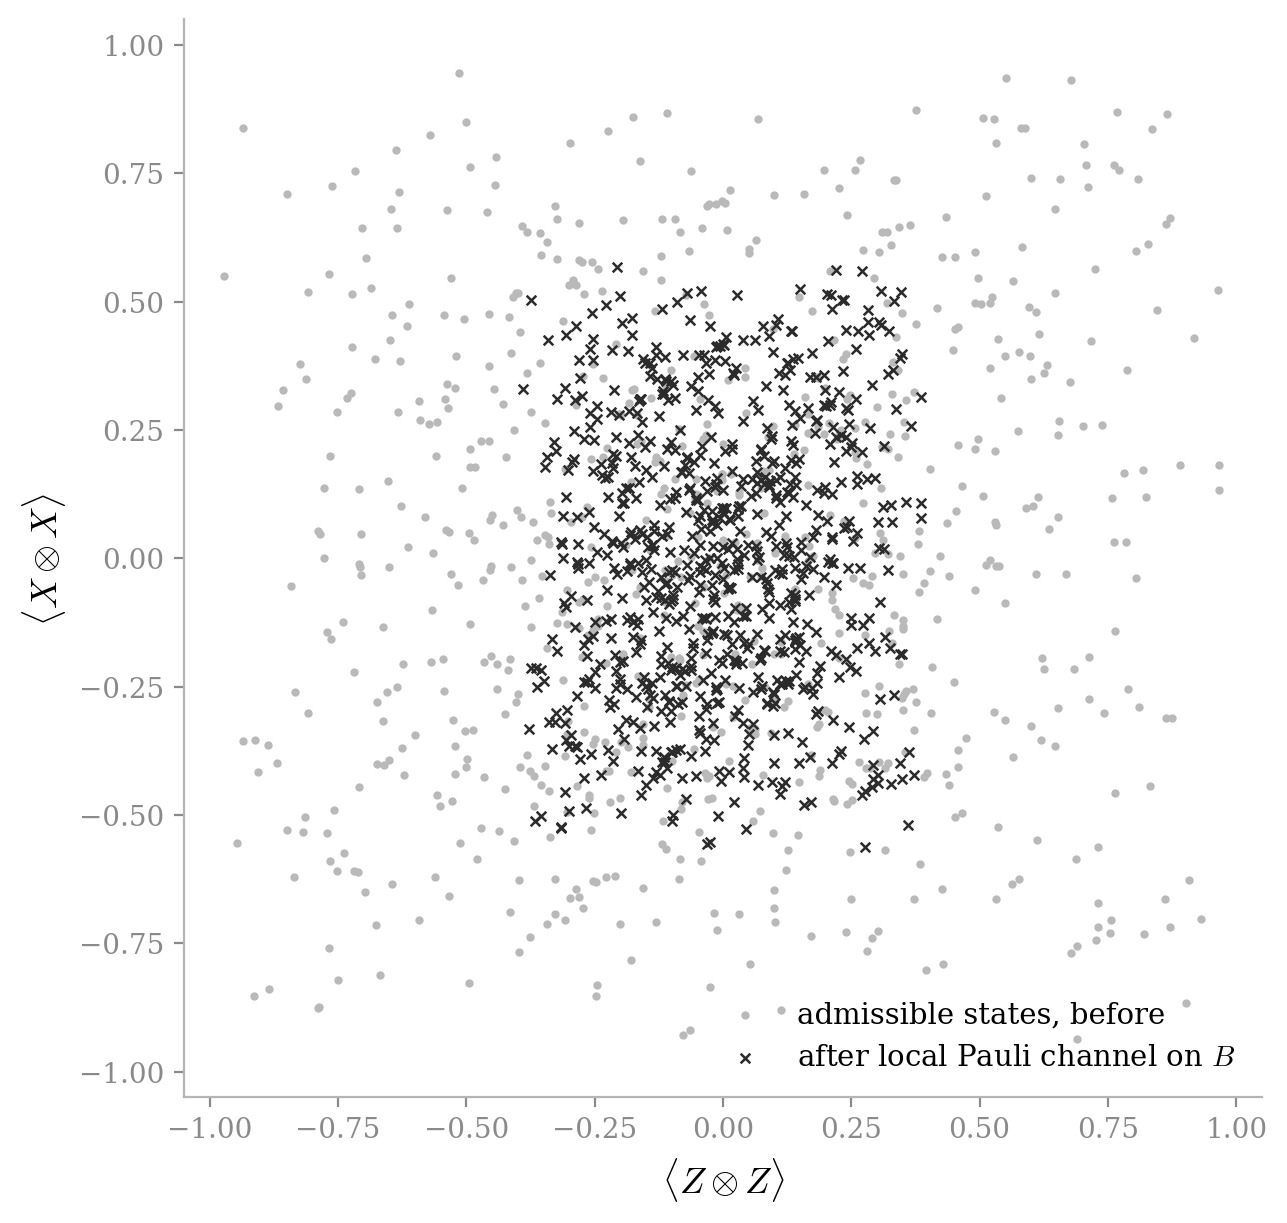
\includegraphics[width=\linewidth,height=0.26\textheight,keepaspectratio]{bell_diagonal_before_after.png}
\caption{Bell-diagonal before/after local map on \(B\).}
\label{fig:corr_no_influence_bell}
\end{subfigure}\hfill
\begin{subfigure}[t]{0.48\textwidth}
\centering
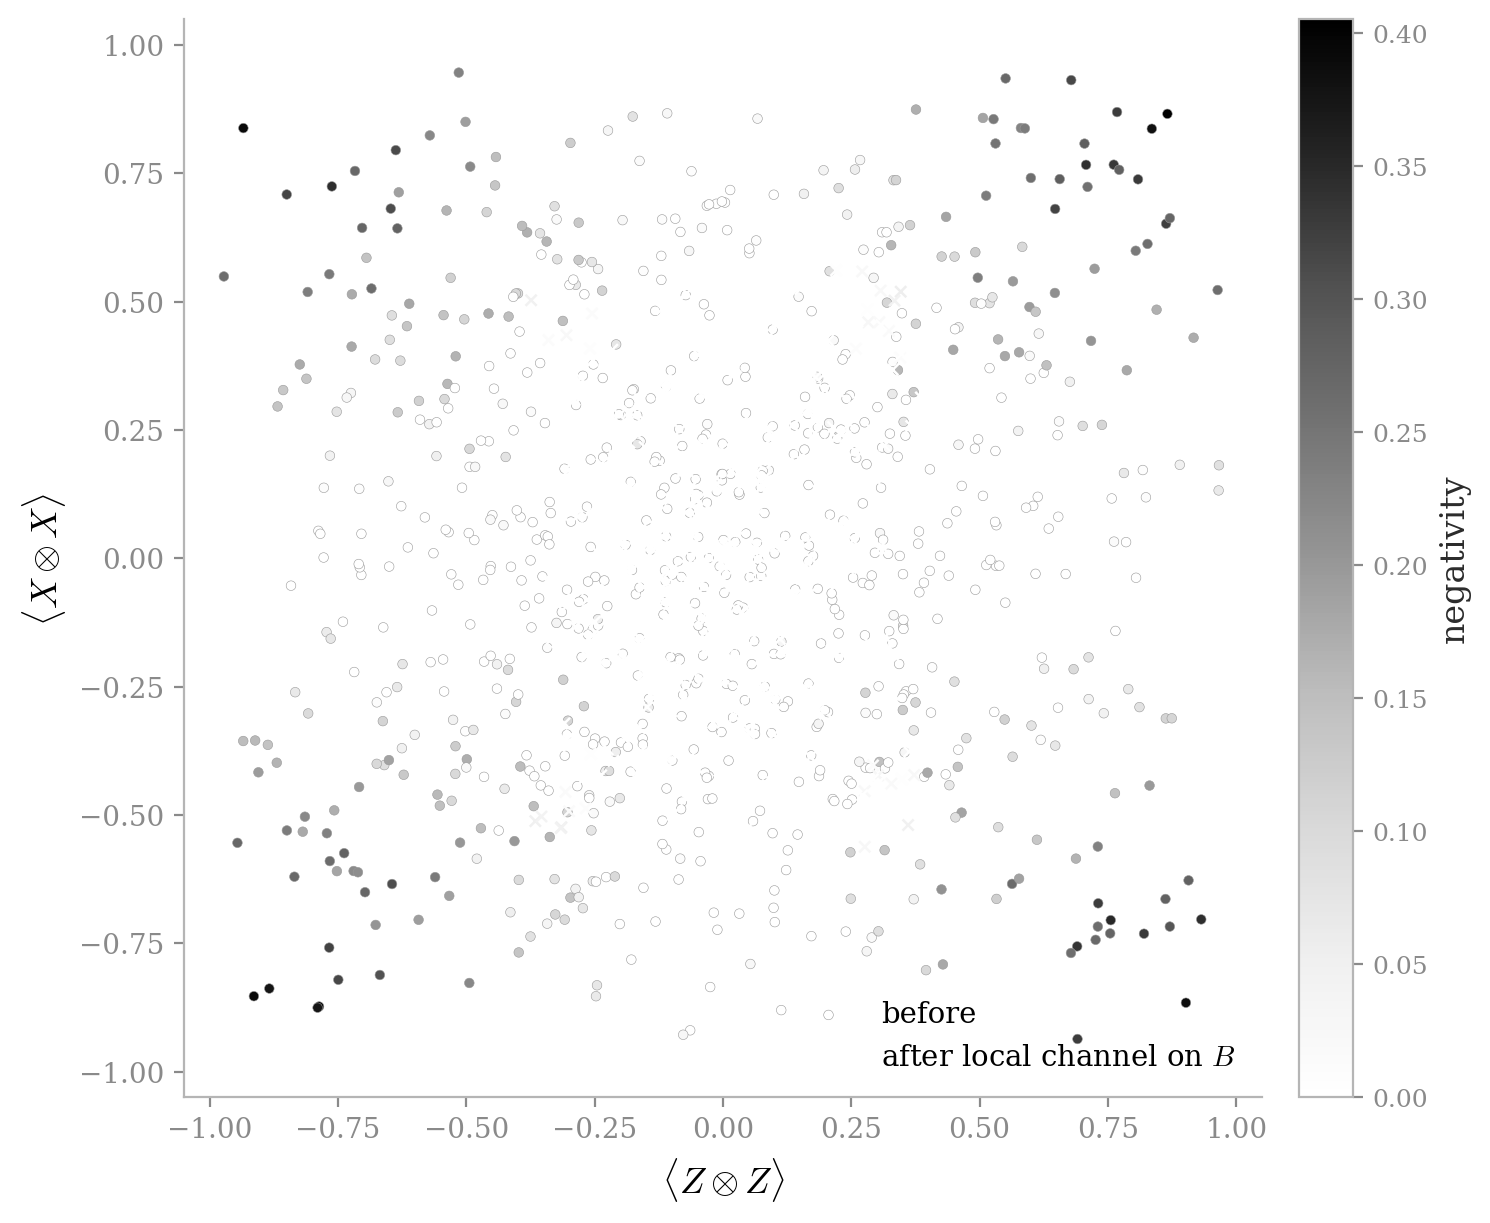
\includegraphics[width=\linewidth,height=0.26\textheight,keepaspectratio]{entanglement_band_negativity.png}
\caption{Same projection, negativity coloring, before and after.}
\label{fig:corr_no_influence_ent}
\end{subfigure}
\captionsetup{justification=raggedright,singlelinecheck=false}
\caption{\textbf{Correlation without influence.}
Left: a local CPTP map on \(B\) changes the joint description while
leaving \(A\)'s marginal invariant. Right: the same projection with
negativity coloring, before (dots) and after (crosses) the local map.
The joint diagnostic moves substantially under the local channel, with
negativity shifts up to \(0.35\) in the plotted ensemble, while
\(A\)'s marginal is invariant to machine precision. Correlation
strength is structural and does not define a control channel.}
\label{fig:corr_no_influence_comparison}
\end{figure}

\begin{figure}[t]
\centering
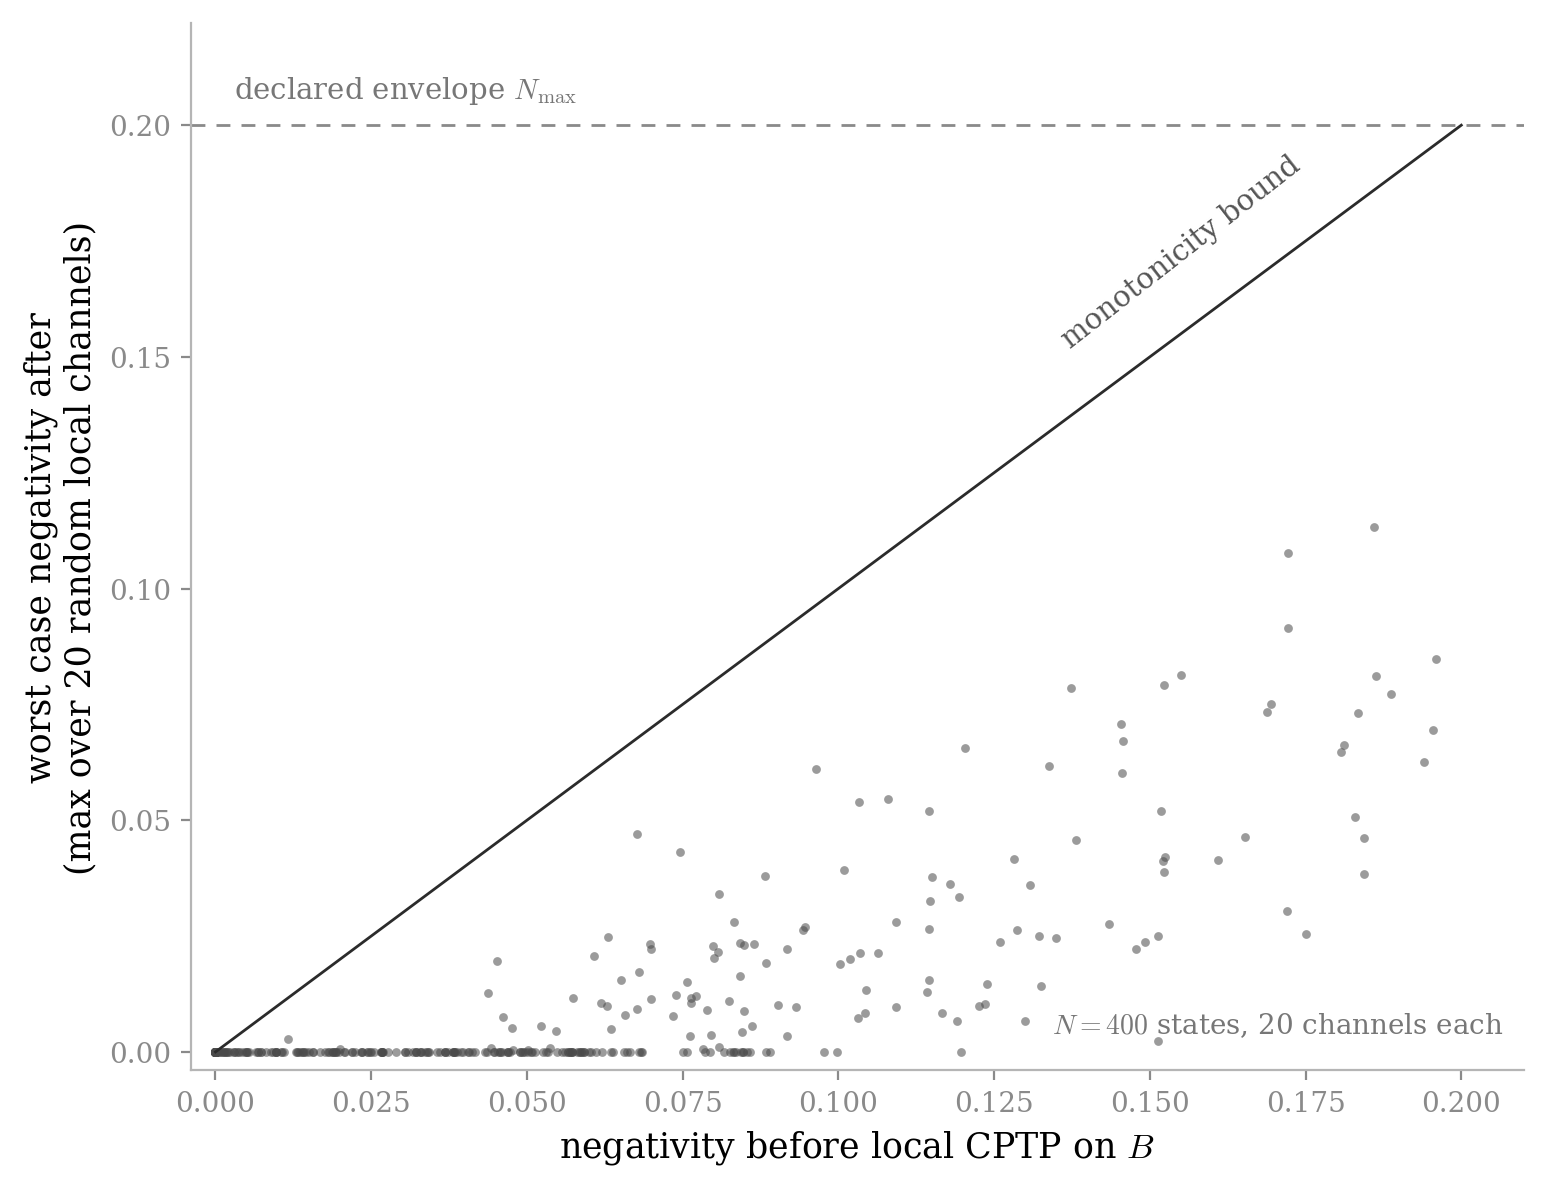
\includegraphics[width=0.72\linewidth]{Onesidedentanglement.png}
\captionsetup{justification=raggedright,singlelinecheck=false}
\caption{\textbf{One-sided local CPTP updating.}
Negativity after an admissible local CPTP map on \(B\) versus initial
negativity, over a Monte Carlo sample of bipartite mixed states
satisfying \(N(\rho_{AB})\leq N_{\max}\). For each state the plotted
after-value is the maximum over twenty independently sampled local
channels; even this worst case lies on or below the diagonal,
reflecting that negativity is non-increasing under local CPTP maps, so
the declared envelope is preserved. The plot is an illustrative
diagnostic: local admissible operations do not create an influence
channel on the distant marginal. No empirical claim is made.}
\label{fig:toy_hardmode_negativity_scatter}
\end{figure}

\paragraph{Axiom unit test.}

\begin{itemize}

\item \textbf{NS1:}
\(\mathcal M_A(E)\) and \(\mathcal M_B(E)\) are indexed only by \(E\);
no map parameters depend on \(\rho_{AB}\), diagnostics, ensemble
decompositions, or outcomes.

\item \textbf{CPTP linearity:}
all updates are linear CPTP; joint updates are product-form. The test
fails if postselection or outcome-conditioned branching is used.

\item \textbf{No outcome-conditioned selection:}
no branching on measurement results is introduced.

\item \textbf{No retro-admissibility:}
no cross-envelope maps are added; only in-domain updating under fixed
\(E\) is represented.

\item \textbf{No influence channel:}
Lemma~\ref{lem:marginal_invariance} enforces marginal independence.
Steering would require local map-family selection to depend on remote
choices, outcomes, or state-conditioned data, which is excluded.

\end{itemize}

The toy also does not retune
\[
\Gamma_E,
\qquad
\mathcal N_E,
\qquad
\mu_E.
\]

\paragraph{Structural takeaway.}

Non-factorizable admissibility can persist while admissible local CPTP
updates leave the distant marginal invariant. Correlation is structural;
influence requires a dependence channel excluded by NS1 and linear CPTP
updating.

\begin{proposition}[Reconstruction relabeling does not alter non-factorization]
\label{prop:nonfact_reconstruction_invariant}
Fix \(E\) and a jointly admissible set
\[
\mathcal A_{AB}(E)\subseteq\Phi_{AB}.
\]
Suppose \(\mathcal A_{AB}(E)\) is non-factorizable over admissible
marginals in the sense of
Eq.~\eqref{eq:nonfactorizable_def_core}. Let \(\mathcal R\) be an
admissible spatial reconstruction dictionary under fixed \(E\) that
assigns representational labels, coordinates, or distance relations to
already-given elements of \(\Phi\), without modifying
\[
\mathcal A_{AB}(E),
\qquad
\mathcal A_A(E),
\qquad
\mathcal A_B(E),
\qquad
\Compat_E,
\]
or the subsystem decomposition.

Then the underlying joint admissible set remains non-factorizable. A
reconstruction may hide or fail to display non-factorization, but it
does not remove it from the admissibility layer.
\end{proposition}

\begin{proof}
Non-factorizability is the existence of at least one
\[
\rho_{AB}\in\mathcal A_{AB}(E)
\]
that is not contained in the separable hull over the induced admissible
marginals, as in Eq.~\eqref{eq:nonfactorizable_def_core}. This is a
set-membership property of \(\mathcal A_{AB}(E)\subseteq\Phi_{AB}\).

By hypothesis, \(\mathcal R\) only assigns representational labels to
already-given configurations and does not alter the admissible sets,
compatibility predicate, or subsystem decomposition. Therefore the same
\(\rho_{AB}\) remains an element of \(\mathcal A_{AB}(E)\), and its
separability status relative to the same \(A|B\) split is unchanged.

Hence the underlying non-factorization remains. The reconstruction may
project away information needed to recognize it, but it does not alter
the admissibility fact.
\end{proof}

\begin{proposition}[Marginal reconstruction is incomplete when joint constraints distinguish same-marginal states]
\label{prop:nonfact_reconstruction_incomplete}
Fix \(E\). Suppose there exist
\[
\rho_{AB},\sigma_{AB}\in\mathcal A_{AB}(E)
\]
such that
\[
\mathrm{Tr}_B(\rho_{AB})
=
\mathrm{Tr}_B(\sigma_{AB}),
\qquad
\mathrm{Tr}_A(\rho_{AB})
=
\mathrm{Tr}_A(\sigma_{AB}),
\]
but \(\rho_{AB}\) and \(\sigma_{AB}\) differ in at least one
joint-level admissibility, compatibility, or diagnostic relation under
fixed \(E\).

Then the reduced descriptions
\[
(\rho_A,\rho_B)
\]
do not determine the full joint compatibility structure of
\[
\mathcal A_{AB}(E).
\]
\end{proposition}

\begin{proof}
The two joint configurations have identical reduced descriptions:
\[
(\rho_A,\rho_B)
\]
is the same for both. Any reconstruction using only the reduced
marginals therefore receives identical input for \(\rho_{AB}\) and
\(\sigma_{AB}\).

By assumption, however, the two configurations differ in at least one
joint-level admissibility, compatibility, or diagnostic relation under
fixed \(E\). Since the marginal-only input is identical in both cases,
that joint-level distinction cannot be recovered from the marginals
alone.

Therefore marginal reconstruction is incomplete for the stated joint
sector.
\end{proof}

\paragraph{Important qualification.}

Non-factorization alone does not imply the hypothesis of
Proposition~\ref{prop:nonfact_reconstruction_incomplete}. For example,
a jointly admissible set containing only a single Bell state is already
non-separable, but contains no pair of same-marginal admissible states
to compare.

Thus the incompleteness claim is conditional: it applies when the joint
sector contains distinct admissible configurations sharing the same
marginals but differing in joint structure.

\paragraph{Forbidden inference.}

The forbidden inference is:
\begin{quote}
If joint admissibility is non-factorizable, then one party can steer or
signal to the other by local choice.
\end{quote}

This inference fails. Correlation is a property of the admissible joint
sector, while influence requires operator-family selection or
state-/outcome-conditioned dependence, both excluded here.

\subsection{Toy Model: Activity Without Leverage}
\label{toy:activity_without_leverage}

\noindent\emph{Axiom target:} Axiom~VII (NS1), leverage discipline.

\paragraph{What this toy shows.}

Several SSAF boundary cases, including vacuum fluctuations,
time-crystalline order, and other ``busy'' regimes, invite a recurrent
category error:
\[
\text{microscopic activity}
\;\Longrightarrow\;
\text{operational leverage}.
\]

This toy blocks that inference. Even when a fixed context supports
persistent variance, nontrivial correlations, or periodic structure, it
does not follow that an admissible cyclic protocol can rectify that
activity into net work, monotone progress, or a control handle.

The activity may be real. The leverage is not thereby licensed.

This toy is complementary to
Toy~\ref{toy:bounded_admissibility_preview}: there, information
about incoming constraints fails to yield an admissible action; here,
internal activity fails to yield an admissible rectification protocol
(Lemma~\ref{lem:variance_not_leverage}). Both block a leverage
inference, through different mechanisms.

\paragraph{Scope.}

This is an activity-without-extractable-leverage toy under linear CPTP
representability. It introduces no hidden reservoirs, no outcome
targeting, no state-conditioned operator selection, no
retro-admissibility, and no optimization principle.

All admissible dependence is indexed by fixed \(E\) and explicit
external controls included in \(E\), in accordance with NS1.

\paragraph{Axiom unit test.}

\begin{itemize}[leftmargin=2em]
\item \textbf{NS1:} all free inputs, including \(H_E\),
\(\mathcal M(E)\), the reference state \(\omega_E\), and what counts as
cyclic, are fixed by \(E\) and explicit controls. No parameter depends
on \(\rho\), outcomes, or state-derived diagnostics.

\item \textbf{CPTP linearity:} every admissible operation is represented
by a linear CPTP map. No nonlinear update, postselected branch, or
outcome-conditioned operation is used.

\item \textbf{No steering channel:} internal activity is not converted
into leverage, because doing so would require leaving the admissible
cyclic protocol class or introducing operator-family selection.

\item \textbf{Domain-of-definition framing:} the no-leverage result is
a constraint on the declared admissible cyclic protocols under fixed
\(E\), not a new dynamical mechanism.
\end{itemize}

\paragraph{Setup.}

Fix \(E\) for a finite-dimensional system with
\[
\Phi=\mathcal D(\mathcal H).
\]
Let \(\mathcal M(E)\) denote the admissible CPTP maps whose parameters
depend only on the classical environment descriptors and explicit
controls included in \(E\).

Introduce a bookkeeping Hamiltonian \(H_E\) associated with the
interface under \(E\). This is part of the accounting convention
specified by \(E\). It is not introduced as a new force law or
primitive dynamical generator.

For any CPTP map \(\Lambda\), define the work-accounting functional
\begin{equation}
W_{\mathrm{ext}}(\Lambda;\rho)
:=
\mathrm{Tr}\!\bigl[H_E(\rho-\Lambda(\rho))\bigr].
\label{eq:toy_work_def}
\end{equation}
Positive \(W_{\mathrm{ext}}\) denotes net work extracted from the
system according to this accounting convention.

\paragraph{Reference state and activity.}

Assume the context admits a distinguished reference state
\[
\omega_E\in\Phi
\]
with:

\begin{enumerate}[label=(\roman*), leftmargin=2em]
\item \textbf{Stationarity:} there exists a nontrivial
\(\mathcal T_E\in\mathcal M(E)\) such that
\[
\mathcal T_E(\omega_E)=\omega_E.
\]

\item \textbf{Activity:} there exists an observable \(X\) with
\[
\mathrm{Var}_{\omega_E}(X)>0,
\]
and/or admissible two-time correlators under \(\mathcal T_E\) are
nontrivial, for example periodic in an effective description.
\end{enumerate}

This captures ``busy'' behavior without committing to a microscopic
mechanism.

\paragraph{Passivity assumption.}

Assume \(\omega_E\) is \emph{passive} with respect to \(H_E\) over the
declared admissible cyclic protocol class. That is, for every cyclic
admissible protocol
\[
\Lambda_{\mathrm{cyc}}\in\mathcal M(E),
\]
where ``cyclic'' means that all external controls included in the
protocol return to their initial values and no additional
nonequilibrium resource is consumed,
\begin{equation}
W_{\mathrm{ext}}(\Lambda_{\mathrm{cyc}};\omega_E)\leq 0.
\label{eq:toy_passivity}
\end{equation}

This is imposed as a boundary condition on admissible operations under
fixed \(E\). It is not derived as a new dynamical law
\cite{Pusz1978,Lenard1978}.

\paragraph{Important qualification.}

The passivity condition does not deny ordinary work extraction from
nonequilibrium states, driven systems, measurement-feedback protocols,
moving boundaries, external reservoirs, or explicitly supplied control
resources. Such cases change the accounting context or add resources to
the protocol.

The toy addresses only the narrower inference:
\[
\text{activity inside the reference state}
\;\Longrightarrow\;
\text{work extraction by an admissible cyclic protocol}.
\]
That inference fails.

\begin{figure}[t]
\centering
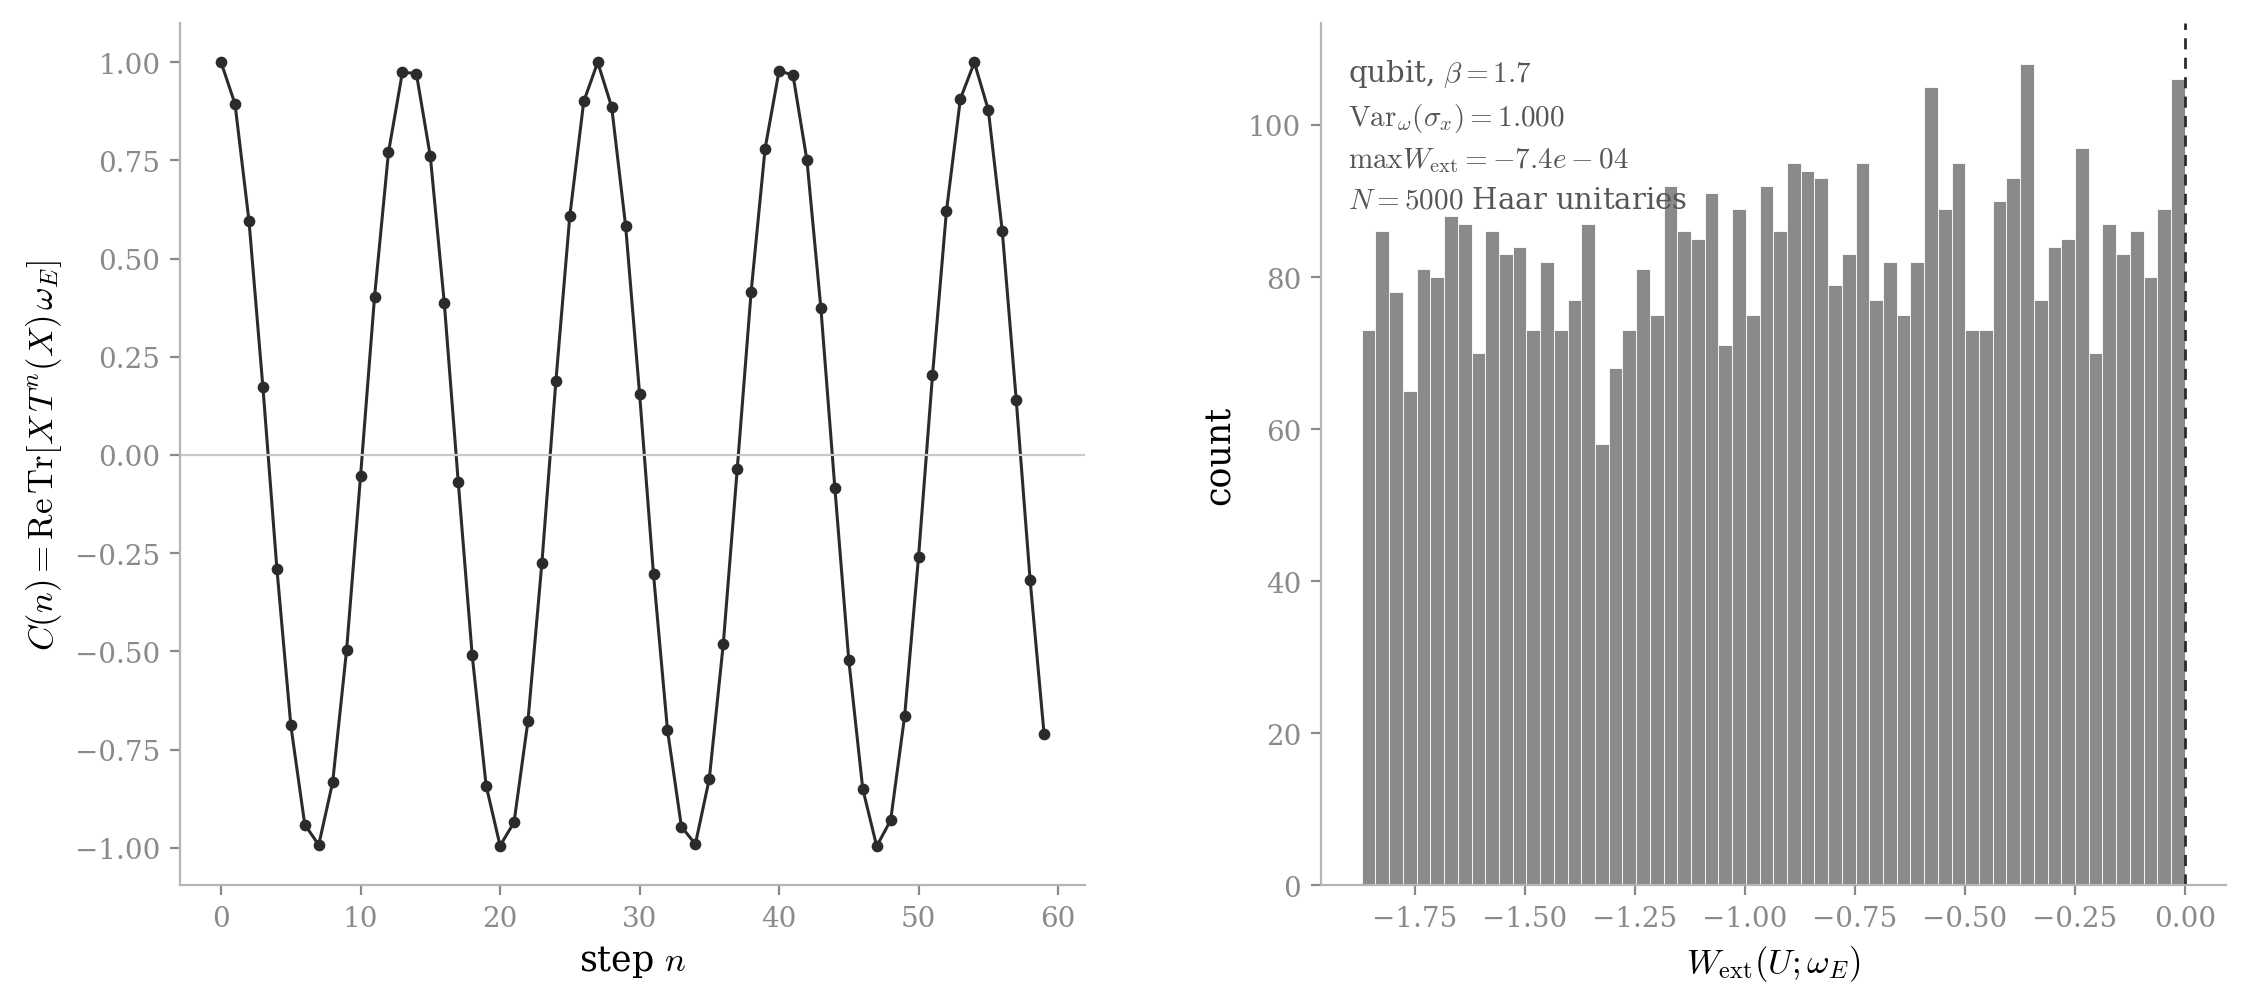
\includegraphics[width=\linewidth]{activity_without_leverage.png}
\captionsetup{justification=raggedright,singlelinecheck=false}
\caption{\textbf{Activity without leverage.} Left: a fixed reference
state shows persistent variance and repeating correlation structure
(``busy'' behavior). Right: sampling cyclic admissible protocols yields
no positive extracted work (histogram remains at
\(W_{\mathrm{ext}}\leq 0\), up to numerical roundoff). The figure
visualizes the toy's point: microscopic activity does not automatically
provide a control handle or net work extraction under fixed \(E\) and
admissible cyclic CPTP operations.}
\label{fig:toy_activity_without_leverage}
\end{figure}

\subsubsection{Variance and Periodicity Do Not Furnish Leverage}
\label{toy:activity_wo_leverage_lemma}

\begin{lemma}[Activity does not imply a rectifiable monotone]
\label{lem:variance_not_leverage}
Under the passivity condition~\eqref{eq:toy_passivity}, the existence
of nonzero variance \(\mathrm{Var}_{\omega_E}(X)>0\) and/or persistent
temporal correlations does not imply the existence of any admissible
cyclic protocol yielding positive extractable work from \(\omega_E\).
\end{lemma}

\begin{proof}
Passivity~\eqref{eq:toy_passivity} constrains all admissible cyclic
protocols under fixed \(E\) to satisfy
\[
W_{\mathrm{ext}}(\Lambda_{\mathrm{cyc}};\omega_E)\leq 0.
\]
Variance and correlation structure are properties of \(\omega_E\) and
of admissible records under the fixed context. They do not alter the
admissible protocol class, the cyclicity condition, or the accounting
functional. Therefore no admissible cyclic protocol in the declared
class can convert the observed activity into positive extracted work.
\qedhere
\end{proof}

The key point is that passivity is a property of the reference state
relative to the admissible protocol class. It constrains what cyclic
protocols are available; it is not a statement that the state lacks
internal structure.

A state can be internally busy, with nonzero variance and persistent
correlations, while still being impossible to exploit through any
admissible cyclic protocol in the declared class.

\paragraph{Periodicity is not progression.}

If admissible records exhibit periodic or quasi-periodic correlation
structure, such as time-crystalline order in an effective description,
that repetition does not define a monotone progression variable
available for operational gain.

Any rectification into positive work would require a cyclic protocol
with
\[
W_{\mathrm{ext}}>0,
\]
contradicting the passivity boundary
\eqref{eq:toy_passivity}.

Attempts to harvest activity by allowing the admissible family or its
parameters to depend on outcomes, internal state, or state-derived
diagnostics constitute state- or outcome-conditioned operator
selection. That violates NS1 and falls outside the admissible scope.

\paragraph{Outcome.}

Under fixed \(E\), and for admissible CPTP operations satisfying the
passivity boundary for cycles, microscopic variance and persistent
correlations do not furnish an admissible work handle or monotone
progression variable.

\paragraph{Forbidden inference.}

The forbidden inference is:
\[
\begin{aligned}
&\text{persistent activity or periodic correlation}
\\
\Longrightarrow\;
&\text{net work, monotone progress, or a control handle}
\\
&\text{by admissible cyclic operation}.
\end{aligned}
\]

This inference fails. Activity is compatible with strict non-leverage
under admissible CPTP protocols in a fixed context.

\subsection{Toy Model: Unified Admissibility Erosion, Filtration Density, and Drift Amplification}
\label{toy:unified_admissibility_erosion}

\noindent\emph{Axiom target:} Axiom~VII (NS1), erosion regime.

\paragraph{Axiom unit test (pass condition).}

Under a specified classical context \(E\), admissibility thresholding,
filtration-density distortion, and clock-drift amplification must be
composable as a single NS1-compliant bookkeeping structure. The
composite may define an effective retention functional, a
momentum-resolved distortion profile, and a drift-amplification
diagnostic, but every parameter must remain indexed by \(E\) or by
explicitly specified context drift \(E_s\), never by the quantum state
\(\rho\), its decomposition, state-derived diagnostics, or outcomes.

\paragraph{What this toy shows.}

The preceding toys establish several structural mechanisms in isolation.
This construction tests whether they can be assembled without breaking
the framework's dependency discipline: local thresholding supplies a
loss fraction, filtration geometry supplies a projected distortion, and
clock reconstruction supplies drift amplification. The result is a
single bookkeeping model for decay-like retention and observable
distortion.

The toy does not introduce a physical decay mechanism. It shows only
that SSAF can represent decay-like summaries using context-indexed
admissibility structure and reconstruction data.

\paragraph{What to avoid.}

Do not read the effective decay rate
\[
\Gamma_{\mathrm{eff}}
\]
as a fundamental dynamical law. It is a derived bookkeeping parameter.
The exponential form of the retention functional is a small-loss
approximation to repeated restriction, not a postulated evolution law.

Do not read \(q^2\), \(\Omega\), or \(\Xi_E\) as new primitives. They
are projection coordinates and distortion summaries chosen inside a
declared reconstruction.

\paragraph{Scope.}

This construction unifies:

\begin{itemize}[leftmargin=2em]
\item local admissibility thresholding;
\item filtration-density distortion;
\item context drift and clock-reconstruction amplification;
\item diagnostic coherence erosion under admissible restriction.
\end{itemize}

It establishes that stable decay-like behavior, localized observable
distortion, drift-induced deviation, and monotone diagnostic erosion can
be represented without primitive time, state-dependent dynamics, or
violations of NS1.

\paragraph{Setup.}

Fix a classical context \(E\). Let \(x\in\mathbb R\) be a local
admissibility coordinate with threshold at \(x=0\). Define the
context-indexed distribution
\begin{equation}
p_E(x)
=
\frac{1}{\sqrt{2\pi}\,\sigma(E)}
\exp\!\left[
-\frac{(x-\mu(E))^2}{2\sigma(E)^2}
\right],
\label{eq:toy_unified_pE}
\end{equation}
and the local loss fraction
\begin{equation}
f(E)
=
\int_{-\infty}^{0}p_E(x)\,dx
=
\Phi\!\left(\frac{-\mu(E)}{\sigma(E)}\right),
\qquad
0\leq f(E)\leq 1.
\label{eq:toy_unified_fE}
\end{equation}

Here \(f(E)\) is a structural loss fraction for the toy threshold. It
is not a probability of outcome selection and not a state-dependent
rate.

\paragraph{Sequencing count and retention.}

Let \(N_E\) denote the number of addressably recorded restriction
markers in a chosen reconstruction window under fixed \(E\). When a
clock reconstruction \(t=R(\tau;E)\) exists, one may write
\[
N_E(t)=r(E)t
\]
as a constant-density approximation. If no such reconstruction is
licensed, \(r(E)\) and the \(t\)-parametrized form below are undefined.

Under the constant-density approximation, define the retention
functional
\begin{equation}
\mathcal R(t;E)
=
\bigl(1-f(E)\bigr)^{r(E)t}.
\label{eq:toy_unified_retention}
\end{equation}
For \(f(E)\ll 1\),
\begin{equation}
\mathcal R(t;E)
\approx
\exp[-r(E)t f(E)].
\label{eq:toy_unified_retention_approx}
\end{equation}

This is a bookkeeping summary of repeated restriction. It is not a
fundamental time evolution law.

\paragraph{Filtration density layer.}

Let the admissibility filtration be indexed by integers:
\begin{equation}
\mathcal F_E
=
(A_0\supset A_1\supset\cdots\supset A_n),
\qquad
\Delta_i:=A_i\setminus A_{i+1}.
\label{eq:toy_unified_filtration}
\end{equation}
Each shell \(\Delta_i\) carries a declared projection characteristic
\[
\chi_i(q^2,\Omega),
\]
where \(q^2\) is squared momentum transfer and
\(\Omega=(\theta_\ell,\phi_\ell)\) is a solid-angle coordinate in the
chosen observable reconstruction. These are projection variables, not
SSAF primitives.

Define the projected filtration density
\begin{equation}
\varrho_E(q^2,\Omega)
=
\sum_i w_i\,\chi_i(q^2,\Omega),
\label{eq:toy_unified_filtration_density}
\end{equation}
and normalized distortion relative to a reference context \(E_0\):
\begin{equation}
\Xi_E(q^2,\Omega)
=
\frac{
\varrho_E(q^2,\Omega)-\varrho_0(q^2,\Omega)
}{
\varrho_0(q^2,\Omega)
},
\label{eq:toy_unified_distortion}
\end{equation}
where the expression is used only on the domain where
\(\varrho_0(q^2,\Omega)\neq 0\).

A convenient toy ansatz is
\begin{equation}
\Xi_E(q^2,\Omega)
=
\varepsilon
\exp\!\left[
-\frac{(q^2-q_0^2)^2}{2\sigma_q^2}
\right]
\Bigl(a_0+a_2P_2(\cos\theta_\ell)\Bigr),
\label{eq:toy_unified_ansatz}
\end{equation}
where \(P_2\) is the second Legendre polynomial. This ansatz is not
part of the framework. It is a compact witness that radial and angular
distortions can be represented in one context-indexed profile.

\paragraph{Effective loss fraction and full retention.}

Define
\begin{equation}
f_{\mathrm{eff}}(E,q^2,\Omega)
=
f(E)\bigl(1+\Xi_E(q^2,\Omega)\bigr).
\label{eq:toy_unified_feff}
\end{equation}
The admissible domain of this toy requires
\begin{equation}
0\leq f_{\mathrm{eff}}(E,q^2,\Omega)\leq 1.
\label{eq:toy_unified_feff_bounds}
\end{equation}
Equivalently, where \(f(E)>0\),
\begin{equation}
-1
\leq
\Xi_E(q^2,\Omega)
\leq
\frac{1}{f(E)}-1.
\label{eq:toy_unified_distortion_bounds}
\end{equation}

Under the small-loss approximation,
\begin{equation}
\mathcal R(t;E,q^2,\Omega)
\approx
\exp\!\left[
-r(E)t\,f(E)\bigl(1+\Xi_E(q^2,\Omega)\bigr)
\right].
\label{eq:toy_unified_retention_full}
\end{equation}

\paragraph{Context deformation.}

Let the context be parametrized as
\[
E=E(T,P).
\]
The admissibility descriptors may inherit \(E\)-dependence through a
declared deformation model:
\begin{align}
\mu(E)
&=
\mu_0-\alpha_T(T-T_0)-\alpha_P(P-P_0),
\nonumber\\
\sigma(E)
&=
\sigma_0+\beta_T|T-T_0|+\beta_P|P-P_0|,
\label{eq:toy_unified_deformation}\\
r(E)
&=
r_0\bigl[1+\gamma_T(T-T_0)+\gamma_P(P-P_0)\bigr].
\nonumber
\end{align}
All dependence is indexed by \(E\). NS1 is preserved because none of
these quantities depends on \(\rho\), state diagnostics, or outcomes.

\paragraph{Context drift extension.}

Let the context vary along a reconstruction label \(s\):
\[
E\longmapsto E_s.
\]
This is context re-indexing, not fixed-\(E\) evolution. Define the
cumulative admissibility-loss functional
\begin{equation}
\Sigma(t,q^2,\Omega)
=
\int_0^t
r(E_s)f(E_s)
\bigl(1+\Xi_{E_s}(q^2,\Omega)\bigr)\,ds,
\label{eq:toy_unified_sigma}
\end{equation}
on intervals where the reconstruction is defined. Then
\begin{equation}
\mathcal R(t,q^2,\Omega)
=
\exp[-\Sigma(t,q^2,\Omega)].
\end{equation}

\paragraph{Amplification and clock reconstruction.}

Let \(t=R(s;E)\) be an operational clock reconstruction with
\begin{equation}
\frac{dt}{ds}=\alpha(E_s),
\qquad
\alpha(E_s)>0.
\end{equation}
For any differentiable descriptor \(a(s)\), the chain rule gives
\begin{equation}
\frac{d^2a}{dt^2}
=
\frac{1}{\alpha^2}\frac{d^2a}{ds^2}
-
\frac{\alpha'(s)}{\alpha(s)^3}
\frac{da}{ds}.
\label{eq:toy_unified_amplification}
\end{equation}
The second term is a reconstruction-drift correction. It is absent
when the clock factor is constant.

Define the amplification witness
\begin{equation}
\mathcal A(s;E)
:=
\left|
\frac{\alpha'(s)}{\alpha(s)^2}
\right|.
\label{eq:toy_unified_amp_factor}
\end{equation}
This measures the fractional change of clock rate per unit
reconstructed time. It is a reconstruction diagnostic, not a force,
source, or dynamical amplification mechanism.

For the effective bookkeeping rate
\begin{equation}
\Gamma_{\mathrm{eff}}(E_s,q^2,\Omega)
:=
r(E_s)f(E_s)
\bigl(1+\Xi_{E_s}(q^2,\Omega)\bigr),
\label{eq:toy_unified_gamma_eff_drift}
\end{equation}
the reconstructed derivative is
\begin{equation}
\frac{d\Gamma_{\mathrm{eff}}}{dt}
=
\frac{1}{\alpha(E_s)}
\frac{d}{ds}
\Bigl[
r(E_s)f(E_s)
\bigl(1+\Xi_{E_s}(q^2,\Omega)\bigr)
\Bigr].
\label{eq:toy_unified_gamma_drift}
\end{equation}
It vanishes for constant \(E\) and is first order in context drift.

Define cumulative amplification over a reconstruction interval by
\begin{equation}
\mathcal A_{\mathrm{cum}}(t)
:=
\int_0^t
\left|
\frac{\alpha'(s)}{\alpha(s)^2}
\right|\,ds.
\label{eq:toy_unified_amp_cumulative}
\end{equation}
This is a monotone diagnostic of accumulated clock-drift distortion,
not a conserved quantity or new physical resource.

\paragraph{Amplification hierarchy.}

Under slow drift, the schematic hierarchy is
\begin{equation}
\begin{gathered}
\text{zeroth order:}\quad
\Gamma_{\mathrm{eff}}(E),
\qquad
\text{first order:}\quad
\frac{d\Gamma_{\mathrm{eff}}}{dt}
=
O\!\left(
\frac{\mathcal A}{\alpha}
\Gamma_{\mathrm{eff}}
\right),
\\
\text{second order:}\quad
\frac{d^2\Gamma_{\mathrm{eff}}}{dt^2}
=
O\!\left(
\frac{\mathcal A^2}{\alpha^2}
\Gamma_{\mathrm{eff}}
\right),
\end{gathered}
\label{eq:toy_unified_amp_hierarchy}
\end{equation}
provided the relevant derivatives exist and the drift expansion is
valid.

The hierarchy is a chain-rule scaling statement. It is not a new
dynamical law.

\paragraph{Connection to the coherence functional.}

The retention functional \(\mathcal R\) may be used as an upper-envelope
bookkeeping descriptor for coherence erosion when the restriction steps
are represented by \(\Delta_E\)-covariant CPTP maps.

Let \(\rho(t)\) denote the state after a reconstructed sequence of
restriction steps under the declared context. If each step is
\(\Delta_E\)-covariant and if the toy loss fraction bounds the
coherence loss per step, then
\begin{equation}
\Coh_E(\rho(t))
\leq
\Coh_E(\rho(0))\,\mathcal R(t;E,q^2,\Omega).
\label{eq:toy_unified_coh_bound}
\end{equation}

The hypotheses in the previous sentence are necessary. Monotonicity of
\(\Coh_E\) under \(\Delta_E\)-covariant CPTP maps guarantees that
coherence does not increase, but it does not by itself fix the
specific envelope \(\mathcal R\). The retention functional is therefore
a model-dependent upper bound, not a universal theorem.

The faithfulness condition
\[
\Coh_E(\rho)=0
\Longleftrightarrow
\Delta_E(\rho)=\rho
\]
ensures that vanishing coherence corresponds to block-diagonality in
the \(E\)-specified reference structure, not merely to an arbitrary
numerical zero.

Throughout, \(\Coh_E\) remains diagnostic. It does not enter
admissibility criteria, map selection, generator coefficients, \(f(E)\),
\(r(E)\), or \(\Xi_E\).

\paragraph{Concrete check.}

The retention functional can be evaluated in the spin-\(\tfrac12\)
\(z\)-dephasing instantiation of Sec.~\ref{sec:zdephasing}. In that
case the toy bookkeeping rate should be calibrated so that
\[
\Gamma_{\mathrm{eff}}(E)
\]
matches the independently derived Lindblad dephasing rate for the same
context, up to the convention-dependent factor relating decay of
\(c(t)\), \(|c(t)|\), and \(\Coh_E\).

This is a consistency check on the toy parametrization. It is not an
independent derivation of the Lindblad rate.

\paragraph{Thermodynamic interpretation (restricted).}

Define the angle-averaged cumulative loss
\begin{equation}
\Sigma_0(t)
=
\int_0^t r(E_s)f(E_s)\,ds,
\label{eq:toy_unified_sigma0}
\end{equation}
obtained from Eq.~\eqref{eq:toy_unified_sigma} by setting
\(\Xi_E=0\).

\(\Sigma_0\) is a monotone bookkeeping measure of cumulative
admissibility loss. It may be read as a structural analogue of entropy
increase only within the declared reconstruction. No thermodynamic
primitive, heat flow, or entropy-production law is introduced.

\paragraph{Result.}

Under NS1-compliant context dependence, the effective bookkeeping rate is
\begin{equation}
\Gamma_{\mathrm{eff}}(E,q^2,\Omega)
=
r(E)f(E)\bigl(1+\Xi_E(q^2,\Omega)\bigr),
\label{eq:toy_unified_gamma_eff}
\end{equation}
subject to
\[
0\leq f(E)\leq 1,
\qquad
0\leq f_{\mathrm{eff}}(E,q^2,\Omega)\leq 1,
\]
with \(f(E)\ll1\) required for the exponential approximation. All
dependence is indexed by \(E\) and projection coordinates, never by
\(\rho\).

\paragraph{Empirical-facing constraints.}

This toy does not generate standalone empirical predictions. It
provides explicit test templates connected to the primary NS1
rate-independence prediction of
Sec.~\ref{subsec:resolution_scaling_hypothesis}.

\begin{description}[leftmargin=2em, style=nextline]

\item[F1. Rate-independence under state variation.]
For fixed \(E\) and fixed observable channel \((q^2,\Omega)\),
\[
\Gamma_{\mathrm{eff}}
\]
contains no \(\rho\)-dependence. Varying \(\rho\) across preparations
must leave the fitted rate statistically unchanged, provided the
independent \(E\)-witness certifies fixed context.

\textit{Violation criterion:} reproducible \(\rho\)-dependent rate
variation under independently confirmed fixed \(E\) and fixed observable
channel.

\item[F2. \(E\)-indexed distortion profile.]
The toy ansatz represents observable distortion as an \(E\)-indexed
profile in \(q^2\) and \(\Omega\). The Gaussian-times-Legendre form is
not mandatory. What is mandatory for the toy is that \(\Xi_E\) be
indexed by \(E\), not by \(\rho\), and that
\[
0\leq f_{\mathrm{eff}}\leq1.
\]

\textit{Violation criterion:} a distortion profile whose angular or
momentum dependence varies reproducibly with \(\rho\) under confirmed
fixed \(E\).

\item[F3. Drift-amplification scaling.]
Under controlled context drift \(E_s\), the clock-drift witness
\[
\mathcal A=\left|\frac{\alpha'}{\alpha^2}\right|
\]
predicts that reconstructed drift corrections scale by chain-rule
factors involving powers of \(1/\alpha\).

\textit{Violation criterion:} measured drift sensitivity incompatible
with the declared reconstruction \(t=R(s;E)\), after confirming that the
drift is in \(E_s\) rather than in \(\rho\).

\end{description}

\paragraph{Status of these constraints.}
Stated plainly, to pre-empt the natural question. F1 is the
discriminating member of the family: standard GKSL practice already
\emph{assumes} state-independent rates, so existing well-characterized
dephasing experiments implicitly support F1 but were not designed to
bound it, and the constraint's content is the certified absence of
\(\rho\)-dependent rate drift at whatever precision a dedicated test
achieves, under an independent fixed-\(E\) witness. To that extent F1
is a consistency test sharpened into a violation criterion rather than
a novel-phenomenon prediction, and accounts permitting
state-conditioned generator selection are the alternatives it
discriminates against. A systematic comparison of F1--F3 against
existing dephasing-rate and drift datasets has not been performed and
is recorded as the immediate empirical next step for this program; no
claim is made here about the precision existing data already reach.

\paragraph{Structural takeaway.}

The framework admits stable decay-like retention under constant \(E\),
localized observable distortion through nonzero \(\Xi_E\),
drift-induced deviation through \(E_s\), and monotone diagnostic
coherence erosion under suitable CPTP restrictions, without primitive
time, state-dependent dynamics, or NS1 violation.

Admissibility geometry determines structural possibility. Sequencing
density, where reconstructable, summarizes restriction count.
Filtration distortion determines projected observable deviation. The
coherence functional tracks diagnostic erosion. The construction shows
that these bookkeeping layers compose without adding new primitives.

\subsection{Summary of Axiom Unit Tests}
\label{toy:summary}

The toy models in this appendix collectively test a single structural
claim from multiple directions: within a fixed classical context \(E\),
the boundary between what is admissible and what is not is a
domain-of-definition boundary, not a dynamical prohibition. A growing
subset of these constructions is additionally machine-verified: their
pass conditions are encoded as executable assertions in the openly
archived verification suite
(\url{https://doi.org/10.5281/zenodo.20634526}).

Across the toys, the same pattern recurs. A map, protocol,
intervention, or reconstruction that appears possible from outside the
description is absent from the admissible class under fixed \(E\). The
ancestor cannot be reached not because reaching it is forbidden, but
because no map in the admissible class has the required domain and
codomain. Cross-envelope reconfiguration is undefined, not suppressed.
The interface trap cannot be escaped not because the system resists,
but because no action satisfies the fiberwise legality condition. The
interior cannot be reconstructed not because of a law against it, but
because the inverse problem has no solution on quotient-accessible data.

The toys sort into five groups by what they test.

\paragraph{Ordering and admissibility structure.}

Sections~\ref{toy:nontotal_ordering}--\ref{toy:structural_nontotal_ordering}
establish that non-total ordering is stable and that incomparability is
structural undefinedness, not missing information
(Lemmas~\ref{lem:toy_no_completion}
and~\ref{lem:toy_no_completion_entailment}). Branching
prerequisite structure arises purely from conditional admissibility
under fixed \(E\), with no dynamics required to explain it.

\paragraph{Sequencing and irreversibility.}

Sections~\ref{toy:finite_dim_sequencing_no_retro}--\ref{toy:single_qubit_NS1_safe_GKSL_semigroup}
establish that retro-admissibility is blocked by non-injectivity of
interface maps or CPTP channels on the relevant domain, that sequencing
is restriction of addressability rather than dynamics, and that
irreversible restriction under NS1-safe updating is represented through
contractivity together with failure of admissible recovery
(Proposition~\ref{prop:no_cptp_recovery},
Lemma~\ref{lem:strict_contraction_no_cptp_recovery}).

\paragraph{Joint admissibility and correlation.}

Sections~\ref{toy:two_qubit_joint_admissibility_without_factorization}--\ref{toy:correlation_without_influence}
establish that entanglement is non-separable joint admissibility under
fixed \(E\), that marginals need not determine joint structure, and that
non-factorizable joint admissibility coexists with absence of influence
between subsystems under product-form local CPTP updating.

\paragraph{Primitive separation and grounding.}

Section~\ref{toy:threshold_shadow_grounding} closes a loop on the
separation entries: the compatibility and connectivity declared in the
charge-sector model
(Sec.~\ref{toy:connectivity_strict_separation}) are recovered
as threshold shadows of one graded access functional, so within that
model class the separated primitives are also grounded primitives, and
the compatibility coherence inclusion holds by construction.

\paragraph{Envelope structure, reconstruction, and leverage.}

Sections~\ref{toy:envelope_bound_resolution_stronger}--\ref{toy:activity_without_leverage}
establish that cross-envelope access is a domain/codomain failure, that
apparent acceleration can arise as a reconstruction artifact of clock
drift, that interface traps cannot be escaped by preview, that interior
structure can be invisible to the interface without ceasing to exist in
\(\Phi\), and that persistent activity does not imply extractable
leverage under a declared passive cyclic protocol class.

\paragraph{Composition and operational constraints.}

Section~\ref{toy:unified_admissibility_erosion} shows how
admissibility thresholding, filtration-density distortion, and
context-drift amplification can be composed into a single
NS1-compliant decay-rate architecture. This toy is unique in the
appendix in producing explicit operational constraints connected to
the paper's primary NS1 rate-independence test
(Sec.~\ref{subsec:resolution_scaling_hypothesis}): rate-independence
under state variation, \(E\)-indexed distortion profiles, and
clock-drift amplification scaling. These constraints are consequences
of the toy ansatz and reconstruction protocol; they do not constitute
independent empirical confirmation of SSAF.

None of these results introduces new dynamics, new primitives, or new
postulates. Each toy shows that a structural feature already present in
the framework--envelope invariance, CPTP contractivity, admissibility
closure, non-injectivity, quotient coarseness, or reconstruction
dependence--is sufficient to block an inference that might otherwise
seem available.

The toys do not add to the theory. They test that the theory does not
secretly require more machinery than it claims.

\section{Appendix E: A Worked Resolution --- The Wavefunction as Interference Structure}
\label{sec:appendixE_worked_resolution}
 
This appendix carries the wavefunction reading of
Sec.~\ref{subsec:wavefunction} through a single explicit case: the
resolution of one qubit under the \(z\)-dephasing context of
Sec.~\ref{sec:zdephasing}. The aim is to show concretely what the
reading does and does not establish. The appendix shows how ordinary
``collapse'' language can be replaced, up to the nonselective
measurement stage, by a context-driven contraction of the admissible
description requiring no dynamical selection rule and no state-dependent
parameter. It also marks the remaining single-outcome problem rather
than concealing it.

\paragraph{The configuration before resolution.}

Work in the spin-\(\tfrac12\) instantiation of
Sec.~\ref{sec:zdephasing}. Let the pre-measurement context \(E\) fix
the \(\sigma_z\) preferred basis, a \(\sigma_z\) readout interface
\(\mathcal O(E)\), and a preparation bound
\[
\varepsilon(E)\geq \frac12
\]
permitting the relevant off-diagonal structure.

Take
\[
|\psi\rangle
=
\frac{1}{\sqrt2}
\left(
|0\rangle+|1\rangle
\right),
\]
with
\begin{equation}
\rho_\psi
=
|\psi\rangle\langle\psi|
=
\begin{pmatrix}
\tfrac12 & \tfrac12 \\[2pt]
\tfrac12 & \tfrac12
\end{pmatrix}.
\label{eq:appendixE_pre_resolution_state}
\end{equation}

Under \(E\), this configuration is admissible: its population satisfies
\[
p=\frac12\in[0,1],
\]
and its off-diagonal magnitude satisfies
\[
|c|=\frac12\leq\varepsilon(E).
\]

In the reading of Sec.~\ref{subsec:wavefunction}, \(\rho_\psi\) is the
complete pure-state configuration under \(E\). It carries the full
phase and interference structure of the system relative to the chosen
chart. The coefficients
\[
c_0=c_1=\frac{1}{\sqrt2}
\]
are chart data for this one configuration. They are not, in this
reading, hidden selections of pre-existing alternatives. Born weights
enter only at the interface-statistical layer through
\[
\mathrm{Tr}(M\rho),
\]
not as an additional ontology of pending outcomes.

\paragraph{The resolving context, specified without reference to the outcome.}

A \(z\)-measurement is represented as a transition
\[
E\to E'
\]
in which the environmental coupling acts to completion. The new context
\(E'\) retains the same preferred basis and readout interface, but takes
the strong-dephasing limit
\[
\varepsilon(E')=0
\]
as in Sec.~\ref{sec:zdephasing}.

The important point is that \(E'\) is fixed by the apparatus and
environment: the readout axis, coupling, pointer basis, and completed
dephasing interaction. It is not fixed by which result is later read.
The specification of \(E'\) can be given before any outcome is known.

This is required by NS1: no parameter entering
\[
E',
\qquad
\mathcal A(E'),
\qquad
\Compat_{E'}
\]
may depend on \(\rho\), an ensemble decomposition of \(\rho\), or a
measurement result. The contraction about to be described is therefore
not state-conditioned or outcome-conditioned.

\paragraph{The contraction of admissible description.}

Under \(E'\), the admissible set contains only diagonal states in the
\(\sigma_z\) basis:
\[
\mathcal A(E')
=
\left\{
\begin{pmatrix}
p & 0\\
0 & 1-p
\end{pmatrix}
:
p\in[0,1]
\right\}.
\]

The pre-resolution coherent configuration \(\rho_\psi\) has
off-diagonal magnitude
\[
|c|=\frac12>0,
\]
so
\[
\rho_\psi\notin\mathcal A(E').
\]

Thus the original coherent configuration is no longer well-posed as an
admissible configuration under the new context. This is the
domain-of-definition event described in Sec.~\ref{subsec:wavefunction}:
the interface vocabulary of \(E'\) no longer licenses the coherent
off-diagonal structure.

When the same physical process is represented by the standard
nonselective \(z\)-dephasing CPTP map, the representative state becomes
\begin{equation}
\rho'
=
\Delta_z(\rho_\psi)
=
\begin{pmatrix}
\tfrac12 & 0 \\[2pt]
0 & \tfrac12
\end{pmatrix}.
\label{eq:appendixE_nonselective_dephased_state}
\end{equation}

This is the classical population mixture inherited from
\(\rho_\psi\). The contraction itself is a restriction of the
admissible description; the dephased density operator \(\rho'\) is the
standard nonselective representative of that restriction. No
outcome-conditioned map is used.

Everything to this point follows from \(E'\) and standard linear CPTP
updating. No single outcome has been selected.

\paragraph{What the contraction does not deliver.}

The contraction under \(E'\) leaves the nonselective mixture
\[
\rho'
=
\frac12|0\rangle\langle0|
+
\frac12|1\rangle\langle1|,
\]
not a single realized outcome.

Both
\[
|0\rangle\langle0|
\qquad
\text{and}
\qquad
|1\rangle\langle1|
\]
are admissible under \(E'\). Under the compatibility predicate of
Sec.~\ref{sec:zdephasing}, compatibility is determined by equality of
the population vector. Since
\[
(1,0)\neq(0,1),
\]
these two pure outcome states lie in distinct compatibility classes.

Selecting one of them as the realized record would require a further
record-level specification distinguishing the \((1,0)\) class from the
\((0,1)\) class. A context describing an already-recorded outcome can
of course be written after the fact, but such a context is
record-indexed. It cannot be used as the pre-outcome rule that selects
which outcome occurs without introducing outcome-conditioned
dependence.

SSAF therefore does not derive single-outcome selection from
\(E\)-data alone. It supplies the nonselective contraction to an
\(E'\)-diagonal mixture, not a sampling rule selecting one member of
that mixture.

\paragraph{Scope of the result.}

The example establishes the distinctively SSAF content and stops at the
honest boundary.

It shows that the superposition-to-mixture transition, the part often
compressed pedagogically into ``collapse onto the measurement basis,''
can be represented as a context-driven contraction of the admissible
description:

\begin{itemize}
\item \(E'\) is fixed by apparatus and environment, not by the result;
\item \(\rho_\psi\) is admissible under \(E\) but not under \(E'\);
\item the nonselective dephased representative \(\rho'\) is diagonal
and carries the inherited populations;
\item no state-conditioned rate, nonlinear collapse map, or
outcome-conditioned update rule is invoked;
\item the pre-resolution state is treated as complete interference
structure, not as an incomplete list of pending alternatives.
\end{itemize}

What the example does not establish is the selection of a single
realized outcome from the resulting mixture. That step cannot be
carried by an \(E\)-specified contraction without adding an
outcome-indexed rule or a further interpretive mechanism.

This residual is not peculiar to SSAF. It is the same boundary faced by
environment-induced decoherence on its own: decoherence explains the
loss of interference and the emergence of an effectively classical
mixture, but it does not by itself explain why one member of that
mixture is the observed record.

SSAF makes this boundary explicit. It reframes collapse as far as a
context-indexed, NS1-compliant account can honestly reach, and marks
single-outcome selection as the open residual it shares with the broader
no-collapse program rather than claiming to dissolve it.

\section{Appendix F: Exploratory Hypotheses on Admissibility and Correspondence}
\label{appF:exploratory_hypotheses}

\paragraph{Scope.}

This appendix collects exploratory hypotheses motivated by SSAF's
structural constraints. None are axioms, primitives, or required
consequences of the framework. Each hypothesis is admissible only
insofar as it can be stated without control, steering, outcome
selection, retro-admissibility, state-dependent updating, or hidden
access-restoration mechanisms.

Any reading that requires those elements is excluded. SSAF's
falsifiable prediction is deliberately not among these hypotheses; it
is stated operationally, with its experimental protocol, in
Section~\ref{subsec:resolution_scaling_hypothesis}.

\paragraph{Notation.}

``Finer'' and ``coarser'' articulation of a reconstructed ordering
description refer only to granularity within a chosen representation.
They imply no primitive time rate, no dynamical speed of time, and no
state-space flow.

Where an ordering label \(\tau\) is not reconstructable, ordering
density is undefined. It is not small, large, slowed, or accelerated.

\subsection{Hypothesis: Breakdown of Kinematic Description in Extreme Coherence Basins}
\label{subsec:boundary_spaghettification}

\paragraph{Hypothesis.}

In sufficiently deep coherence basins, reconstructed clock description
may become ill-posed: the framework may cease to license a
time-extended kinematic ordering of interior configurations. Interior
narratives that presuppose continuous motion, progressive deformation,
or process-level evolution are then not licensed by the
admissibility/addressability structure.

In plain terms: deep enough inside an extreme coherence basin, the
question ``what is happening step by step?'' may have no defined answer
within the fixed-\(E\) description.

\paragraph{Non-claims.}

This does not assert that time stops ontologically. It is a statement
about addressability and reconstruction. Where \(\tau\) is not
reconstructable, time-extended interior description is undefined.

In exterior reconstructions that do assign a clock parameter, apparent
``freezing'' may correspond to a loss or thinning of addressable
ordering markers relative to the chosen reconstruction protocol. This
is a reconstruction effect, not a new interior process.

No claim is made that interior ordering density tends to zero or
infinity. If the required markers are not addressable, the relevant
density is undefined.

\paragraph{Minimal formalization.}

Let
\[
\{E_r\}
\]
be a family of basin-local context descriptions indexed by nesting depth
\(r\). Assume that for
\[
r\in[r_b,r_0]
\]
the interface relation \(\sim_{E_r}\) admits multiple addressability
classes, but that for
\[
r<r_b
\]
it degenerates to a single addressable class over the interior sector.

In the degenerate region, no admissible sequencing chain of distinct
addressable configurations is defined. Kinematic descriptions fail by
domain-of-definition, not by dynamical prohibition.

\paragraph{Illustrative mappings.}

The following phrases are permitted only as descriptive projections
under a stated interface:

\begin{enumerate}[label=(\roman*), leftmargin=2.2em]
\item ``horizon-like boundary'' = non-addressability interface;
\item ``information persistence'' = existence at the \(\Phi\) level,
or record-level persistence without cross-addressability;
\item ``spaghettification'' = boundary-resolved admissibility reduction
across an extended object's interface;
\item ``null-admissibility basin'' = limiting description in which no
persistent identity description remains sequencing-addressable.
\end{enumerate}

None of these mappings introduces a spacetime singularity, an interior
dynamics, or a bulk-boundary reconstruction principle.

\subsection{Hypothesis: Envelope-Bounded Tunneling}
\label{subsec:hyp_envelope_tunneling}

\paragraph{Hypothesis.}

Phenomena described as tunneling may admit an SSAF translation as
envelope-bounded compatibility between configurations sharing
admissible phase relations across an effective barrier. Under this
reading, tunneling is not literal traversal through an obstacle but
re-description within a compatibility envelope whose admissible
relations are not captured by the coarse barrier narrative.

\paragraph{Structural boundary.}

This reading fails if interpreted as controlled traversal, targeted
transport, selective passage, feedback, or outcome-conditioned tuning.

It also fails if the envelope is treated as a hidden channel carrying
energy, information, or agency across a barrier.

\paragraph{Significance.}

This blocks barrier-as-obstacle narratives without adding transport,
hidden reservoirs, or control channels, while remaining consistent with
non-extractability constraints~\cite{Landauer1961,Pusz1978}.

\subsection{Hypothesis: Nonlocal Correspondence Without Agency}
\label{subsec:hyp_nonlocal_correspondence}

\paragraph{Hypothesis.}

Nonlocal correlations may admit description as correspondence between
jointly admissible configurations without implying communication,
influence, or agency. Correspondence reflects shared constraints within
\(\Phi\), not signal transfer.

\paragraph{Structural boundary.}

This reading fails if treated as a communication channel, influence
mechanism, steering resource, or intentional interaction.

\paragraph{Significance.}

This separates correspondence from causation while preserving standard
no-signalling constraints~\cite{Bell1964,Tsirelson1980,Gisin1990}.

\subsection{Hypothesis: Descriptive Bridges Between Admissibility Regimes}
\label{subsec:hyp_descriptive_bridges}

\paragraph{Hypothesis.}

Apparent ``bridges'' between effective regimes may arise as descriptive
mappings between compatibility structures rather than causal
connections. These bridges do not transmit information, energy, matter,
or intent, and do not permit feedback, traversal, or control.

\paragraph{Structural boundary.}

This reading fails if a bridge is treated as a physical channel,
traversal path, wormhole mechanism, reconstructible interior mapping, or
access-restoration operation.

\paragraph{Significance.}

This permits descriptive continuity across regimes while forbidding
illicit interior reconstruction or shortcut channels. References to
wormhole or holographic language are analogical only; no ER--EPR,
bulk-boundary duality, or holographic reconstruction claim is adopted
here~\cite{Susskind1993,Susskind1995}.

\subsection{Hypothesis: Admissibility Sweeps}
\label{subsec:hyp_admissibility_sweeps}

\paragraph{Hypothesis.}

Changes in classical environmental constraints may induce
\emph{admissibility sweeps}: context re-indexings
\[
E\longmapsto E'
\]
that alter which configurations are jointly admissible within the new
description. A sweep is therefore a global re-description of
admissibility structure under changed classical conditions, not a
within-\(E\) control operation.

\paragraph{Structural boundary.}

This fails if sweeps are treated as tunable, targetable,
feedback-driven, or usable for steering or outcome selection.

Interpretive hygiene:
\[
\text{sweep}\neq\text{steering},
\qquad
\text{change}\neq\text{control}.
\]

A sweep may alter \(\mathcal A(E)\) only by replacing the context index
with a specified new context \(E'\). It does not retune
\(\mathcal A(E)\) from inside fixed \(E\).

\paragraph{Significance.}

This gives language for global reconfiguration under environmental
descriptors without importing agency, outcome targeting, nonlinear
updates, or state-conditioned dynamics~\cite{Lindblad1976,Gorini1976,Zurek2003}.

\subsection{Hypothesis: Phase-Signature Induction}
\label{hyp:phase_signature_induction_format}

\paragraph{Hypothesis.}

Fix \(E\) and interface \(\mathcal O(E)\) with addressability relation
\(\sim_E\). Any realized sequencing description under fixed \(E\) may
admit a context-dependent \emph{phase-signature} labeling map
\begin{equation}
\Sigma_E:\mathcal A(E)\longrightarrow \mathsf{Sig}_E,
\label{eq:phase_signature_map_H}
\end{equation}
into a signature space \(\mathsf{Sig}_E\), satisfying:

\begin{enumerate}[label=(\roman*), leftmargin=2.2em]
\item \(\Sigma_E\) is indexed only by classical/interface descriptors
in \(E\);
\item \(\Sigma_E\) is constant on addressability classes:
\[
\rho\sim_E\sigma
\Longrightarrow
\Sigma_E(\rho)=\Sigma_E(\sigma);
\]
\item on any declared addressable subdomain where distinct records must
be separated, \(\Sigma_E\) may be chosen to refine the quotient labels:
\begin{equation}
\rho,\sigma\in\mathcal A(E),
\quad
\rho\not\sim_E\sigma
\quad
\Longrightarrow
\quad
\Sigma_E(\rho)\neq\Sigma_E(\sigma),
\label{eq:signature_refines_H}
\end{equation}
provided that such refinement is part of the stated interface
description.
\end{enumerate}

The minimal construction is simply
\[
\Sigma_E(\rho):=[\rho]_E.
\]
Thus the hypothesis introduces no new ontic variable; it names an
optional quotient-labeling convention.

If \(\sim_E\) is trivial on the relevant domain, then
\(\mathsf{Sig}_E\) is necessarily singleton for that domain.

\paragraph{Structural boundary.}

Phase signatures are record-level invariants, not additional ontic
variables. They do not solve outcome selection, do not restore
non-addressable distinctions, and do not create access beyond
\(\mathcal O(E)\).

No spacetime primitives, internal evolution law, outcome-conditioned
selection, retro-admissibility, or hidden discriminator is introduced.

Once a configuration becomes non-addressable within a realized chain,
its signature is likewise non-addressable within that chain.

\paragraph{Significance.}

The hypothesis supplies a compact language for record labels compatible
with admissibility and addressability. It can support an ordered family
of registered signature classes suitable for reconstructing an emergent
time parameter where such reconstruction is already licensed.

It does not close the single-outcome problem. It labels records within
a realized description; it does not derive why one record rather than
another is realized.

\paragraph{Guardrails.}

All dependence is through \(E\). There are no \(\rho\)-indexed
diagnostics, no outcome-conditioned postselection, no outcome selection,
no retro-admissibility, no spacetime primitive, and no dynamics
smuggling.

\paragraph{Multipartite signatures.}

For bipartite splits \((A,B)\), a factorized signature description may
be represented by a specified embedding
\[
J_E:\mathsf{Sig}^A_E\times\mathsf{Sig}^B_E
\longrightarrow
\mathsf{Sig}^{AB}_E
\]
such that
\begin{equation}
\Sigma^{AB}_E(\rho_{AB})
=
J_E\!\left(
\Sigma^A_E(\rho_A),
\Sigma^B_E(\rho_B)
\right).
\label{eq:signature_factorization_H}
\end{equation}

Failure of Eq.~\eqref{eq:signature_factorization_H} for some jointly
admissible \(\rho_{AB}\) is a signature-level witness of
non-factorized record structure under \(E\). It is not, by itself,
equivalent to entanglement unless the signature map has been specified
to faithfully represent the relevant joint admissibility structure.

Thus multipartite signatures provide a bookkeeping witness, not a new
criterion for nonlocality, influence, or outcome-level independence.

\subsection{Hypothesis: Fractal-Like Constraint Geometry}
\label{hyp:fractal_joint_admissibility}

\paragraph{Hypothesis.}

For physically relevant families of diagnostic interfaces at increasing
resolution, the induced admissibility/compatibility relations on
\(\Phi\) may exhibit approximate scale recurrence: similar constraint
motifs may reappear across refinement levels. In plain terms, the
pattern of which configurations are jointly admissible may look similar
at different descriptive scales, the way a fractal looks similar at
different magnifications.

This is a representational claim about induced constraint patterns,
not an ontological statement about \(\Phi\).

\paragraph{Correlation by exclusion.}

For composite \(AB\) under fixed \(E\), non-factorizability of
\[
\mathcal A_{AB}(E)
\]
under repeated refinement may reproduce similar exclusion patterns
across scales. Entanglement-like correlations would then appear as a
structural consequence of recurring joint-constraint motifs rather than
spatial proximity or signal transfer.

\paragraph{Structural boundary.}

This does not assert that \(\Phi\) carries a primitive metric, topology,
or distance relation. It also does not assert that fractals are
primitive constituents. No outcome steering, retro-admissibility, or
state-dependent updating is introduced.

\paragraph{Status.}

This is a working hypothesis motivated by structural compatibility with
SSAF primitives. No dedicated empirical program has yet been constructed
to evaluate scale recurrence in induced constraint signatures.

\subsection{Hypothesis: Recursive Stratification}
\label{subsec:hyp_recursive_stratification}

\paragraph{Hypothesis.}

Admissible configuration classes may admit nested closure relations
defined solely by admissibility structure across environment-indexed
interfaces \(\mathrm{Obs}(E)\). In plain terms, admissible
configurations may organize into nested layers, where each layer is
incompatible with others in the sense that no single-interface
reparameterization connects them.

\paragraph{Structural boundary.}

This hypothesis fails if the apparent classes can be connected by a
single observer-level reparameterization, such as smoothly widening a
tolerance band or rescaling a diagnostic coordinate, while preserving
the same underlying addressability structure. In that case, the
separation is diagnostic convenience, not structural stratification.

\paragraph{Significance.}

If true, recursive stratification licenses talk of distinct ordering
regimes without importing new dynamics: regime separation is a feature
of admissibility incompatibility, not a phase transition or control
knob.

If false, SSAF should collapse its regime language into a single
diagnostic continuum with explicit tolerance conventions.

\paragraph{Relation to existing structural concepts.}

As a formal pattern, this resembles settings where admissible states
separate into families divided by incompatibility rather than smooth
interpolation, including superselection sectors, topological phases,
renormalization-group fixed points, and environment-induced decoherence
sectors. The comparison is organizational only.

\paragraph{Status.}

This is a hypothesis-check, not a framework commitment. If a single
diagnostic parameterization suffices globally, stratification should be
removed or demoted to commentary.

\paragraph{Open problem: cosmological acceleration without a primitive constant.}

SSAF admits no cosmological constant as a primitive. Whether observed
cosmological acceleration can be represented by the organization of
admissibility structure across scales, rather than by a constant
inserted by hand, is a question the framework raises but does not
answer.

As a formal analogy, this sits near backreaction and averaging programs
in which acceleration-like behavior is associated with inhomogeneous
structure rather than a primitive constant. SSAF's contribution here is
framing only. Recursive stratification is representational and
non-dynamical in the present paper, and Appendix~\ref{app:no_mechanism_substitution}
prohibits converting it into an effective source.

Therefore SSAF makes no cosmological prediction here. It records only
that, on its primitives, a primitive constant is not required to be
\emph{assumed}; whether it can be \emph{avoided} is left open.

\paragraph{Open problem: structure of admissible correlations.}

SSAF accommodates non-factorizable joint admissibility and NS1 prevents
such correlations from becoming signalling channels. However, the
framework does not yet derive the specific boundary of the quantum
correlation set.

In particular, the quantum set is smaller than the full no-signalling
set. Within SSAF, the question is concrete: do CPTP linearity, NS1, and
the compatibility/envelope structure constrain jointly admissible
correlations under fixed \(E\) to exactly the quantum set, or is an
additional structural input required?

If the axioms suffice, Tsirelson-type bounds should be derivable from
admissibility constraints alone. If they do not, identifying the missing
constraint, and determining whether it is already implicit in the
phase-based ordering structure or must be added explicitly, would be a
significant extension of the framework.

\subsubsection{Scope Limitation}
\label{subsec:hyp_scope_limitation}

These hypotheses are interpretive probes only. SSAF does not require
their realization and remains internally complete whether all, some, or
none ever correspond to physical phenomena. Any hypothesis that requires
new primitives, state-conditioned updating, outcome selection,
retro-admissibility, hidden access restoration, or controllable
steering lies outside the framework unless explicitly promoted by a
future theory change.

\section{Appendix G: Boundary Conditions (Structural Limits and Non-Addressability)}
\label{app:boundary_conditions_limits}

\subsection{Constraint: No Mechanism Substitution}
\label{app:no_mechanism_substitution}

SSAF licenses only its fixed primitives and their structural relations:
context-indexed admissibility and compatibility on
\[
\Phi,
\]
irreversible sequencing as non-retro-addressability within a realized
ordering, and, when updating is represented, linear CPTP maps subject
to NS1.

Descriptive correspondences to familiar physical phenomena do
\emph{not} license additional causal agents, effective forces,
propagating influences, optimization principles, variational rules,
teleological criteria, or outcome-indexed selection mechanisms. Any
such addition constitutes a theory change.

In particular, basin language, envelope language, compatibility
language, and reconstruction language are not mechanisms. A basin is
not a force. An envelope is not a barrier with a hidden transport
channel. Compatibility is not attraction. Reconstruction drift is not a
source term. Addressability loss is not an active erasure process.

Any argument that replaces admissibility, envelope closure, or
interface-level addressability with an external driver, an implied
optimization principle, a basin ``force,'' a hidden channel, or a
state-conditioned steering rule falls outside the axiom set.

\subsection{NS1 Constraint on Represented Resolution Operators}
\label{subsec:resolution_operator_families_ns1}

When admissible updating is represented using GKSL/Lindblad form under
fixed \(E\), denote the representational package by
\[
\mathcal L(E)
:=
\{(L_\alpha(E),\lambda_\alpha(E))\}_\alpha .
\]
This is bookkeeping for a linear CPTP family consistent with NS1. It is
not a primitive of SSAF.

\paragraph{NS1 constraint.}

Fix \(E\). No admissible in-domain description licenses selection,
modification, or conditioning of \(\mathcal L(E)\) based on
\[
\rho,
\]
any ensemble decomposition of \(\rho\), any state functional including
coherence measures, any outcome-indexed data, or any record-dependent
selection rule not already specified as part of the fixed context.

Equivalently,
\[
\lambda_\alpha=F_\alpha(E),
\qquad
\frac{\delta\lambda_\alpha}{\delta\rho}=0.
\]

A single fixed \(E\)-indexed representation may include local,
nonlocal, memory-bearing, or correlated Lindblad/GKSL operators acting
on multipartite configurations, provided their full specification is
part of \(E\) and is not selected from the realized state, outcome, or
record history. Such correlations are permitted as fixed
representational structure and do not introduce signalling,
state-dependent tuning, or outcome-conditioned updating.

Any proposal requiring adaptive operator selection,
outcome-conditioned reparameterization, state-functional feedback, or
retroactive modification of the represented family under fixed \(E\)
violates NS1.

\subsection{Apparent Time-Freezing as Loss of Reconstructability}
\label{subsubsec:time_freezing_nonaddressability}

\paragraph{Status.}

Interpretive compression only. No new postulate, structure, or
empirical claim.

In SSAF, ``time'' is an observer-level reconstruction introduced after
a realized sequencing relation is fixed under \(E\). Claims that time
``slows,'' ``freezes,'' or ``stops'' are restated as claims about which
ordering distinctions remain reconstructable from a stated interface
under \(E\).

For sufficiently restrictive contexts, ordering-relevant distinctions
may become non-addressable at a fixed interface even when the
underlying admissibility structure remains well-defined. The quotient
\[
\Phi/{\sim_E}
\]
can become too coarse to support the diagnostic markers required for
clock reconstruction.

In that regime, reconstructed temporal description is undefined. The
claim is not that an interior clock rate becomes zero, nor that
ordering density becomes small or infinite. If the markers required to
define the reconstruction are absent, the reconstruction fails.

``Frozen time'' is therefore shorthand for loss of reconstructability,
not loss of admissible structure and not dynamical arrest.

This is purely structural and NS1-compatible. Any represented updating
remains linear CPTP with parameters indexed only by \(E\). In such
contexts, addressability of spatial or boundary-level descriptors may
persist while ordering markers required for temporal reconstruction do
not. This reflects the non-linkage of spatial and temporal
reconstructions as distinct projections from different diagnostic
inputs.

\subsection{Boundary Cases and Structural Limits}
\label{appG:boundary_cases_intro}

\paragraph{Purpose.}

The boundary cases here introduce no new phenomena or mechanisms. They
function as structural stress tests: regimes where familiar dynamical,
kinematic, or control-oriented questions cease to be well-posed while
SSAF's admissibility, envelope, compatibility, and non-addressability
machinery remains defined.

They sharpen the separation between structural compatibility under
fixed \(E\) and operational access through a stated interface.

\paragraph{What these cases are not.}

None supply controllable degrees of freedom, optimization principles,
hidden channels, engineering prescriptions, or new resource
conversion rules. Apparent protection, persistence, nonlocal
correlation, unusual stability, or boundary localization is read as
fixed context-indexed admissibility/compatibility structure under NS1,
not adaptive stabilization, active intervention, or state-conditioned
modification of admissibility rules.

\paragraph{Why they are needed.}

SSAF's divergence from standard language is structural, not cosmetic.
Entire classes of operations that are well-posed in spacetime-primitive
or mechanism-first descriptions--cross-history intervention,
state-conditioned steering, retro-admissibility, outcome targeting,
hidden reconstruction, and access restoration--are not forbidden
add-ons in SSAF. They are undefined because the requisite admissibility,
compatibility, or ordering objects are not introduced.

Boundary cases make these undefined regions explicit and prevent
effective descriptions from being mistaken for new mechanisms.

\subsection{Boundary Case: Null-Admissibility Basins}
\label{appG:null_admissibility_basins}

\paragraph{Scope.}

No new postulates, mechanisms, or dynamical laws are introduced. This
boundary case specifies a limit of addressable ordering: a regime in
which basin language remains meaningful as a description of
admissibility geometry, while no identity-level description remains
sequencing-reconstructable under fixed \(E\).

The term \emph{null-admissibility basin} is therefore shorthand for
null addressability of identity-preserving continuation, not literal
nonexistence of configurations in \(\Phi\).

\paragraph{Structural characterization.}

Fix \(E\) with admissible set
\[
\mathcal A(E),
\]
compatibility predicate
\[
\Compat_E,
\]
and observational equivalence relation
\[
\sim_E.
\]

A \emph{null-admissibility basin} denotes a limiting regime in which,
for any identity-level description one attempts to track, the
corresponding admissible continuation within \(\mathcal A(E)\) is either
empty or collapses to a \(\sim_E\)-trivial equivalence class.

This is a statement about loss of nontrivial addressable support for
identity-preserving ordering. It is not an existential claim about
individual configurations.

In this limit, no nontrivial sequencing continuation can be stated
within the basin as an in-domain relation on \(\mathcal A(E)\). The
required ordering or identity markers are absent, rather than blocked
by an added prohibition. Configurations may remain elements of
\(\Phi\), and some may remain members of \(\mathcal A(E)\), but no
configuration is licensed as a nontrivial identity-preserving
continuation of the realized ordering under fixed \(E\).

\paragraph{What fails and what does not.}

What fails is sequencing-accessible persistence: no
interface-addressable identifier allows an identity description to
remain reconstructable across the boundary under fixed \(E\).

What does not fail is operational consistency. No singular dynamics,
breakdown of positivity, or violation of linear CPTP representability
is asserted~\cite{Lindblad1976,Gorini1976}.

\paragraph{Domain-of-definition, not singularity.}

Null-admissibility is not a spacetime horizon, curvature pathology,
divergent generator, or force-based narrative. It is a structural
statement about which ordering and identity distinctions remain present
in
\[
\mathcal A(E)
\]
and nontrivial in
\[
\Phi/{\sim_E}
\]
under the stated interface.

If the interface quotient collapses all identity-relevant distinctions,
then an identity-level continuation claim has no defined in-domain
content. The correct conclusion is not that a dynamical process destroys
identity, but that the identity-continuation predicate is no longer
licensed.

\paragraph{No sequencing channel for influence.}

Because no nontrivial identity-preserving continuation is licensed
in-domain at the null-admissibility limit, SSAF supplies no sequencing
channel for control, transport, tuning, rectification, or intervention.

Any interpretation that treats the limit as an operational resource
implicitly introduces state-conditioned access or hidden
addressability-restoration and is outside the framework.

Any attempt to recover addressability across the limit by conditioning
on realized state, desired identity marker, or diagnostic functional
introduces state-dependent resolution dependence and violates
NS1~\cite{Gisin1989,Gisin1990}.

\paragraph{Summary.}

A null-admissibility basin is a structural limit where identity-level
sequencing terminates by non-addressability. Nothing fails dynamically.
The ordering and identity description has no nontrivial in-domain
support in
\[
\mathcal A(E)
\]
or
\[
\Phi/{\sim_E}
\]
under the fixed constraint profile.

Persistence in \(\Phi\) may remain while interface-level
reconstructability of identity-preserving continuation vanishes.

\subsection{Boundary Case: Time Crystals Without Extractable Progression}
\label{subsubsec:time_crystals_no_progress}

\paragraph{Scope.}

Guardrail only. No claim is made that time-crystalline order generates
usable time flow, energy extraction, monotone progression, or any
operational control channel. This boundary case is included only to
sharpen the distinction between persistent structure and
sequencing-level reconstructability.

\paragraph{Background.}

Time-crystalline phases exhibit stable temporal correlations under
fixed constraints. Their defining feature is not ``motion through
time'' but persistence of periodic order in an effective description.

Spontaneous time-translation symmetry breaking as a ground- or
thermal-equilibrium property is not permitted in the usual sense, while
driven Floquet settings admit discrete time-crystalline order under
appropriate stability conditions~\cite{Wilczek2012,Bruno2013NoGoTimeCrystals,
WatanabeOshikawa2015,ElseBauerNayak2016Floquet}.

\paragraph{What this blocks.}

Within SSAF, time crystals exemplify \emph{persistence without
sequencing leverage}: a periodic correlation structure may remain
stable while providing no admissible route for upgrading correlation
into reconstructable progress, extractable work, or outcome-indexed
control.

Periodicity alone does not reopen addressability, does not imply
retro-admissibility, and does not supply a theory-internal selection
rule for realized ordering.

Any interpretation that treats periodic correlation as a control
primitive requires state- or outcome-conditioned dependence of
admissibility, map-family selection, or represented resolution rules.
Such dependence is excluded by NS1 and linear CPTP representability.

Repetition may be present in the effective description while remaining
non-rectifiable in the admissible-ordering sense~\cite{WatanabeOshikawa2015,
ElseBauerNayak2016Floquet}.

\paragraph{Relation to activity without leverage.}

This boundary case is a concrete instance of the activity-without-
leverage principle of Sec.~\ref{toy:activity_without_leverage}.
A system may exhibit persistent variance, recurring correlations, or
periodic order while no admissible cyclic protocol extracts net work or
defines a monotone progression variable under fixed \(E\).

\paragraph{Summary.}

Order is not leverage. A system may sustain regular temporal
correlations while offering no admissible route to a monotone
progression variable, no reopening of addressability, and no in-domain
handle for outcome-targeted modification of realized ordering.

Treating periodicity as an operational knob constitutes a theory change
that violates NS1 and CPTP guardrails~\cite{WatanabeOshikawa2015,
ElseBauerNayak2016Floquet}.

\subsection{Boundary Case: Frozen Entanglement Without Signalling}
\label{subsec:frozen_entanglement_boundary}

\paragraph{Scope.}

This boundary case concerns correlation persistence in the absence of
any sequencing-accessible influence or communication channel. All
statements concern joint admissibility, NS1 discipline, and the
separation between global constraint structure and locally addressable
operations.

No claim is made that entanglement is dynamically frozen in an absolute
sense. ``Frozen'' means unavailable as a local influence channel under
the stated interface and fixed \(E\).

\paragraph{Structural characterization.}

``Frozen entanglement'' refers to regimes in which nonclassical
correlations persist between subsystems while no admissible sequencing
relation licenses cross-subsystem influence.

In SSAF terms, correlated configurations occupy a non-factorizable
joint admissibility envelope in
\[
\Phi_{AB},
\]
yet the operational quotient relevant to local actions provides no map
by which a local intervention on one subsystem yields an addressable
change in the admissible continuations of the other.

Such correlations are accounted as shared compatibility constraints in
the joint description, not as interaction, propagation, or hidden
communication. Correlation persistence is a property of admissibility
structure, not a process-level conduit.

\paragraph{No cross-subsystem influence under NS1.}

Fix \(E\). Under NS1, represented updating uses linear CPTP maps with
parameters indexed only by \(E\), never by the quantum state, distant
settings, outcomes, ensemble decompositions, or state-derived
diagnostics.

For product-form local updating, distant marginals remain invariant
under remote local CPTP operations, as shown in
Sec.~\ref{toy:correlation_without_influence}. More general fixed
joint CPTP structure may encode correlations as part of \(E\), but it
does not license state-dependent or outcome-conditioned signalling.

Changes in descriptive state assignment across subsystems reflect
representational updating on available records, not modification of the
underlying admissibility structure by a distant choice.

Joint compatibility constraints may be global in \(\Phi\), while
operational influence remains excluded because restriction and updating
dependence is fixed entirely by \(E\).

\paragraph{Exclusion of control interpretations.}

This boundary case excludes interpretations that treat entanglement as
a usable channel for instantaneous influence, steering, outcome
selection, or outcome-conditioned coordination.

Any reading that does so requires non-NS1 dependence and violates CPTP
and causal-consistency constraints.

\paragraph{Summary.}

Frozen entanglement is persistent correlation without a signalling
channel. Within SSAF, entanglement is shared joint-admissibility
structure, not a conduit for action or information transfer.

Global relational structure may persist in admissibility without
granting any locally addressable operation that exploits it.

\subsection{Boundary Case: Decoherence-Free Subspaces Without Isolation}
\label{subsec:dfs_boundary}

\paragraph{Scope.}

DFS is treated here as a structural boundary case within SSAF:
stability of an admissible sector under a fixed represented update
family, without requiring physical isolation, internal control,
adaptive feedback, or theory-internal tuning.

All statements concern invariant support under linear CPTP
representability and NS1~\cite{Lindblad1976,Gorini1976}.

\paragraph{Structural characterization.}

Fix \(E\) and a corresponding fixed \(E\)-indexed CPTP update family
\[
\{\mathcal T^E_\Delta\}_\Delta .
\]

A decoherence-free subspace or sector is a subset
\[
\mathcal D_E\subseteq \Phi
\]
such that configurations supported on \(\mathcal D_E\) remain supported
on \(\mathcal D_E\) under the fixed update family:
\[
\rho\in\mathcal D_E
\quad\Longrightarrow\quad
\mathcal T^E_\Delta(\rho)\in\mathcal D_E
\]
for the relevant admissible labels \(\Delta\), possibly up to unitary
rotation within the sector~\cite{Zanardi1997,Lidar1998}.

In SSAF terms, this invariance is a compatibility relation between a
subset of \(\Phi\) and the fixed restriction/update structure indexed
by \(E\). It is not, by itself, a claim that the system is physically
decoupled from the environment.

\paragraph{Stability without isolation.}

DFS persistence does not require zero environmental coupling. The same
\(E\)-indexed update rule may act on the full admissible domain, while
a particular sector remains invariant because the noise operators act
trivially, collectively, or unitarily on that sector.

Thus the stability is structural: the fixed represented update family
has no admissible image taking configurations out of the sector. The
sector is not actively defended. It is invariant under the declared
operation class.

In SSAF language, this means that escape descriptions are not licensed
by the fixed \(E\)-indexed update structure. That is stronger than
saying the interface merely fails to observe escape; the represented
maps themselves preserve the sector.

\paragraph{Exclusion of tuning interpretations.}

DFS excludes readings in which the system selects, maintains, or
engineers the invariant sector through an internal rule. Any such
reading introduces forbidden dependence: state-conditioned
operator-family choice, outcome-indexed restriction, or adaptive
parameter updates.

External engineering techniques may exist as physical practices, but
they enter SSAF only by changing the classical context
\[
E\longmapsto E',
\]
not as theory-internal controls under fixed \(E\).

\paragraph{Summary.}

Decoherence-free subspaces illustrate that long-lived coherence may
arise without isolation, internal control, or adaptive tuning. Within
SSAF, this stability is attributed to invariant support under a fixed
linear CPTP representation with NS1 dependency discipline.

Persistence reflects invariant admissible structure, not active
protection.

\paragraph{Three boundary cases together.}

Time-crystalline behavior exhibits periodic correlation without
extractable progression. Frozen entanglement exhibits stable
correlation without signalling. DFS exhibits invariant admissible
structure under environmental coupling.

Together these cases separate correlation, persistence, and operational
addressability, preventing them from being conflated as a single
resource. In each case the interesting behavior is real: the
correlation, the periodicity, or the stability. What does not follow is
operational leverage.

\subsection{Boundary Case: Many-Body Localization Without Control}
\label{subsec:mbl_boundary}

\paragraph{Scope.}

MBL is treated as an illustrative regime of long-lived local order
without theory-internal control, protected access, or active
stabilization. All statements are translated into SSAF terms:
context-indexed admissibility and compatibility,
sequencing-accessible reachability under a stated interface, and
linear CPTP representability subject to NS1.

This boundary case is interpretive. It does not assert that MBL is
stable under arbitrary open-system noise, nor that SSAF derives MBL
from first principles.

\paragraph{Background.}

Many-body localization refers to regimes in which interacting
many-body systems fail to approach thermal equilibrium over accessible
scales, with local ordering and correlations persisting without ordinary
thermal relaxation~\cite{Basko2006,Nandkishore2015}. Microscopic
evolution continues while macroscopic equilibration is absent or
strongly delayed on the relevant scales.

\paragraph{SSAF reading.}

Within SSAF, MBL exemplifies \emph{persistence by restricted
reachability}. Under fixed \(E\), the sequencing-accessible region of
the admissible set remains narrowly constrained by many-body
compatibility relations. The effective behavior is persistence of local
ordering descriptors without exploration of the admissible sectors that
would support an equilibrium coarse-grained description.

In plain terms: the system continues to have structure and internal
activity, but the accessible continuations remain local or constrained.
The broader thermalizing descriptions are not licensed under the fixed
context and stated interface.

\paragraph{Persistence without thermalization.}

Persistence does not require active protection, error correction, or an
internal memory mechanism. The stated interface supplies no addressable
set of transitions sufficient to disperse local ordering into a
thermalized description class.

Thermalization fails here as absence of licensed reachability sufficient
to justify equilibrium-style coarse graining under fixed \(E\), not as
a dynamical stoppage.

\paragraph{Entropy and reachability.}

In MBL-like regimes, effective entropy growth may be suppressed because
the sequencing-accessible region remains small relative to the abstract
configuration volume~\cite{Serbyn2013,Huse2014}.

The entropy proxy in SSAF tracks sequencing-accessible variety under a
stated interface. It is not a count of all abstract states in
\[
\Phi.
\]

\paragraph{Exclusion of memory and control interpretations.}

MBL does not license interpretations that treat persistence as
controllable memory storage or as a selectable information register
inside SSAF.

Physical platforms may use localization-like stability for memory in
engineering contexts, but such use requires an explicitly specified
control and readout protocol. SSAF does not introduce a theory-internal
rule that selects, retains, or manipulates ordering patterns through
state- or outcome-conditioned dependence.

Persistence is attributed solely to fixed compatibility and reachability
constraints under the stated context and interface.

\paragraph{Summary.}

Many-body localization illustrates persistence without thermalization
or theory-internal control. Within SSAF, this is restricted
reachability: the sequencing-accessible region remains narrow under the
fixed context and stated interface.

Ordering persists not by protection or choice, but because dispersion
pathways are not licensed as addressable within the reconstructed
description.

\subsection{Boundary Case: Quantum Scars Without Optimization}
\label{subsec:quantum_scars_boundary}

\paragraph{Scope.}

Quantum scars are treated as an illustrative regime of recurrent
ordering patterns without teleology, optimization, or hidden guidance.
All statements concern admissibility and compatibility constraints,
unified stratification, and linear CPTP representability with NS1 under
fixed \(E\).

No goal-directed principle, selection rule, variational driver, or
trajectory-guidance mechanism is introduced.

\paragraph{Background.}

Quantum scars denote recurrence or enhanced weight of particular state
families in systems otherwise expected to exhibit ergodic
behavior~\cite{Heller1984,Turner2018}. They appear as repeated
concentration of ordering along specific configuration families without
ordinary symmetry protection, integrability, or an extensive set of
conserved quantities.

\paragraph{SSAF reading.}

Within SSAF, scars are read as \emph{recurrence under restricted
reachability}. Certain ordering families remain jointly compatible
across stratification layers while many abstractly available
alternatives are not licensed as jointly admissible under fixed \(E\).

The prominence of scarred families is attributed to residual
compatibility, not preference, attraction, or optimization.

In plain terms: these patterns recur not because the system is aiming
at them, but because the fixed admissibility and compatibility
structure leaves fewer addressable alternatives than a fully ergodic
description would suggest.

\paragraph{Recurrence without optimization.}

Scars require no minimized functional, extremal principle, or
trajectory-guidance rule inside SSAF. Recurrence arises because the
admissible and reachable class is restricted: many alternative
continuations are absent from the in-domain description, excluded by
compatibility constraints, or rendered \(\sim_E\)-trivial.

Recurrence is residual structure under constraint, not motion toward a
target.

\paragraph{Unified stratification and leftover compatibility.}

Scarred families persist because they remain compatible across multiple
stratification layers without invoking sector-specific rules,
auxiliary organizing principles, or hidden optimization criteria.

Apparent structure is residue of constraint, not an added teleological
ingredient. This reinforces SSAF's non-teleological commitment:
ordering is constrained, not goal-directed.

\paragraph{Exclusion of teleological interpretations.}

Quantum scars do not license goal-directed readings. Recurrence does
not imply selection, convergence, or optimization. It reflects repeated
intersection of admissibility and reachability within a restricted
family.

Any interpretation that treats scars as evidence of hidden guidance,
least-action selection, trajectory optimization, or preferred outcome
selection introduces additional primitives and is excluded.

\paragraph{Summary.}

Quantum scars illustrate recurrence without optimization. Within SSAF,
certain ordering patterns reappear not because they are favored, but
because many alternatives are not licensed as jointly admissible under
the fixed context.

\paragraph{The boundary cases together.}

Null-admissibility basins mark where identity-level sequencing
terminates by non-addressability. Time crystals exhibit periodic
correlation without extractable progression. Frozen entanglement
exhibits stable correlation without signalling. DFS exhibits invariant
admissible structure under environmental coupling. MBL exhibits
persistence by restricted reachability without thermalization. Quantum
scars exhibit recurrence without optimization or invariance.

In each case the interesting behavior--stability, correlation,
recurrence, persistence, or periodicity--is structurally real. What is
absent is leverage: no operational handle is thereby supplied for
control, extraction, steering, or outcome targeting.

The boundary cases do not forbid these phenomena. They locate the line
between structural fact and operational availability.

\subsection{Boundary Case: Vacuum Fluctuations Without Extractable Work}
\label{subsec:vacuum_fluctuations_boundary}

\paragraph{Scope.}

This boundary case separates microscopic variance from operational
leverage. It does not deny vacuum fluctuations. It fixes what is
\emph{not licensed}: an inference from vacuum variance to standalone
work extraction under admissible cyclic operations.

\paragraph{Background.}

Vacuum fluctuations denote persistent variance of quantum observables
even in the absence of classical driving, thermal gradients, or
particle excitations. They appear through transient correlations and
boundary-condition-dependent mode reorganization, including
Casimir-type effects~\cite{Casimir1948}.

\paragraph{SSAF reading.}

Within SSAF, vacuum variance is compatible with unresolved structure in
\(\Phi\), but it does not by itself constitute an operational resource.
The boundary claim is not
\[
\text{variance does not exist}.
\]
The boundary claim is
\[
\text{variance does not license an admissible work reservoir}.
\]

Vacuum variance supplies no sequencing-accessible route to directed
output or net work extraction under admissible cyclic protocols. Under
linear CPTP operations indexed by fixed \(E\) and respecting the
relevant equilibrium or passive-state conditions, passivity results
exclude net work extraction from equilibrium states by cyclic
processes~\cite{Pusz1978,Lenard1978}.

Activity may persist while remaining non-rectifiable into a monotone
work variable unless an external nonequilibrium resource, boundary
change, measurement-feedback channel, or control asymmetry is explicitly
introduced.

\paragraph{Casimir-type effects.}

Casimir-type phenomena arise from boundary-condition-dependent
reorganization of modes, not from treating vacuum fluctuations as a
freely harvestable work reservoir~\cite{Casimir1948}. Moving
boundaries, imposed constraints, or external apparatus changes are part
of the classical context and accounting. They are not zero-cost
extraction channels.

Any scheme that purports to rectify vacuum activity into net work
without importing nonequilibrium structure, boundary work,
measurement-feedback resources, or another operational asymmetry
requires an inadmissible leverage mechanism and violates the passive
cyclic-protocol boundary~\cite{Pusz1978,Lenard1978}.

\paragraph{Summary.}

Vacuum fluctuations correspond to unresolved admissible structure that
does not license a standalone work reservoir under admissible
operations. The vacuum may be active, but it provides no in-domain
protocol for harvesting net work.

Variance is not permission.

\subsection{Boundary Condition: Higgs-Compatibility Non-Exemption}
\label{subsec:higgs_boundary}

\paragraph{What this boundary condition is for.}

SSAF's admissibility framework makes claims about which descriptions are
licensed under fixed \(E\). A recurring category error in applying SSAF
language to physical phenomena is to treat ``persistence with inertia''
as something that could be preserved while selectively bypassing the
compatibility requirements associated with inertial mass in established
particle physics.

This boundary condition names and blocks that move. It is not a
mass-generation model and does not rederive, replace, or modify the
Higgs mechanism~\cite{Higgs1964,Englert1964,ATLAS2012,CMS2012}.

\paragraph{Boundary statement.}

Inertial response and mass-like behavior of known matter are described,
within the Standard Model, through the relevant mass-generation and
coupling structure, including Higgs-sector couplings where
applicable~\cite{ATLAS2012,CMS2012}. In SSAF terms, any description
that treats persistence with inertia as a stable identity-level property
must remain compatible with a fixed, context-indexed constraint profile
\(E\).

SSAF introduces no locally decouplable, selectively bypassable, or
outcome-conditioned exemption rule for that inertial-compatibility
requirement.

Persistence-with-inertia therefore carries a fixed compatibility
requirement. That requirement is structural, not a tunable resource and
not an operational degree of freedom. SSAF may license probes that
alter, destabilize, or destroy the persistence description, but it does
not license an operation that preserves stable identity and inertial
response while exempting the associated compatibility condition.

\paragraph{What this blocks.}

Any proposed extension that licenses operationally controllable inertia
suppression, mass negation, selective Higgs-decoupling as a knob, or
``free'' persistence without the associated compatibility requirement
commits a category error.

Such readings introduce an exemption rule not present in SSAF. If the
exemption is selected by state, outcome, target, diagnostic, or desired
trajectory, it violates NS1.

\paragraph{Failure mode table.}

Table~\ref{tab:category_errors_failure_modes} lists common category
errors and their structural failure modes under fixed \(E\).

\begin{table*}[t]
\centering
\caption{Common category errors and their SSAF failure modes under
fixed context \(E\).}
\label{tab:category_errors_failure_modes}
\begin{tabular}{p{0.46\textwidth} p{0.46\textwidth}}
\toprule
\textbf{Proposed interpretation or claim}
&
\textbf{Structural failure mode} \\
\midrule

Selective inertia suppression
&
Introduces an exemption rule preserving
\(\mathsf{PersistInertia}\) while bypassing the associated
compatibility requirement \(K(E)\); no such in-domain map is licensed.
\\[0.35em]

Thrustless propulsion via field manipulation
&
Requires a control map that selectively alters inertial response while
preserving identity; entails state- or outcome-conditioned dependence
or additional primitives, violating NS1.
\\[0.35em]

Vacuum energy extraction for work
&
Confuses variance with an admissible work reservoir; violates
passivity under admissible cyclic CPTP protocols when no external
nonequilibrium resource is supplied~\cite{Pusz1978,Lenard1978}.
\\[0.35em]

Phase-based mass negation
&
Assumes stable identity persistence with inertial response while
exempting the inertial-compatibility requirement; this is precisely the
non-exemption boundary.
\\[0.35em]

Nonlocal control or steering
&
Requires outcome-conditioned admissibility or nonlinear update
dependence; incompatible with CPTP linearity and
NS1~\cite{Gisin1989,Gisin1990}.
\\[0.35em]

Feedback-driven destination targeting
&
Implements outcome-indexed reweighting or retro-addressable sequencing;
excluded by non-retro-addressability.
\\[0.35em]

Engineering access to prior realized sequences
&
Attempts to reopen addressability of realized ordering chains; violates
terminality of sequencing.
\\[0.35em]

Field tuning as a physical knob
&
Reifies descriptive parameterization as an operational retuning map;
SSAF introduces no in-domain knobs that reweight admissibility or
exempt \(K(E)\).
\\
\bottomrule
\end{tabular}
\end{table*}

\paragraph{Interpretive summary.}

All excluded failure modes share the same structural error: a fixed
persistence constraint is treated as a manipulable resource via a
selective exemption map.

SSAF permits descriptive mappings and effective projections, but it
does not introduce operational control rules that grant outcome-targeted
exemptions. Where a proposal requires steering, state- or
outcome-conditioned reparameterization, or selective bypass of \(K(E)\)
while retaining \(\mathsf{PersistInertia}\), it fails structurally
rather than empirically.

\subsection{Boundary Case: High-Energy Probing Without Field Retuning}
\label{app:boundary_high_energy}

\paragraph{Scope.}

High-energy collisions are a boundary stress test. They explore
admissibility under extreme kinematic and interaction settings while
leaving the admissibility rules of the present formulation unchanged.

The question is not what can be produced transiently, but what cannot
be made persistent without introducing an additional operational
retuning map beyond NS1 and the Higgs-compatibility non-exemption
boundary.

\paragraph{Empirical constraint.}

Modern accelerators access center-of-mass energies and momentum
transfers sufficient to excite rare, short-lived configurations and
directly probe symmetry-breaking structure, including observation of
the Higgs boson~\cite{ATLAS2012,CMS2012}. Across wide variation in
incident energy, geometry, polarization, and interaction channel,
observed outcomes remain describable within stable effective field
theory constraints: produced configurations either persist within
known coherence and stability bounds or decay/terminate according to
the allowed channels~\cite{PeskinSchroeder,Weinberg1995}.

\paragraph{Structural interpretation in SSAF.}

In SSAF, collider experiments function as \emph{admissibility probes}.
They alter which configurations are tested, through phase alignment,
spin orientation, mode occupation, collision energy, and channel
participation, within a stated experimental context.

Collision parameters explore
\[
\text{what is admissible under the specified context},
\]
but do not constitute an admissible operation that modifies
\[
\text{what governs admissibility}.
\]

Changing beam energy, detector geometry, polarization, or interaction
channel changes the experimental context being probed. It does not
supply a theory-internal map that retunes admissibility rules inside a
fixed \(E\).

\paragraph{Relation to Higgs-compatibility non-exemption.}

This aligns with the Higgs-compatibility non-exemption boundary:
persistence with inertia is not treated as a freely separable resource.
Energy injection may disrupt composite ordering, populate unstable
modes, or access higher-mass excitations, but it does not license a
configuration that retains stable identity and inertial response while
exempting the associated compatibility requirements of the relevant
particle-physics description~\cite{Higgs1964,Englert1964}.

This is not a claim that SSAF derives the Standard Model mass structure.
It is a guardrail: SSAF does not introduce a bypass operation that
selectively preserves persistence while exempting the inertial
compatibility conditions already built into the physical description.

\paragraph{Degrees of freedom and structural invariance.}

Collider parameters are coordinates of exploration, not
theory-internal control variables. Increasing energy or changing
scattering geometry changes the subset of configurations tested for
compatibility. It does not relax the conditions required for
persistence.

Observed stability across accessible regimes is therefore read as
compatibility with fixed structural constraints, not as a dynamical
recovery mechanism and not as evidence of an admissibility-retuning
knob.

\paragraph{Persistence as a boundary outcome.}

Configurations persist only when they satisfy the relevant
compatibility conditions for the stated context. Configurations that do
not satisfy those conditions decay, scatter, fragment, or fail to admit
a stable continuation.

Observed stability reflects the absence of continuation paths outside
the persistence envelope, not equilibration, damping, or hidden control.

\paragraph{Failure mode: energy-as-control fallacy.}

A recurring interpretive error treats energy density, collision
geometry, or relativistic velocity as operational controls capable of
modifying persistence, inertia, or admissibility structure itself.

In SSAF, this is a structural failure. Energy changes which
configurations are tested. It does not, by itself, change the
admissibility constraints. Any proposal that requires collision
parameters to implement an additional retuning or exemption map
violates NS1 and the Higgs-compatibility non-exemption boundary.

\paragraph{Relation to other boundary cases.}

This case coheres with the vacuum-fluctuation boundary, inertia
non-exemption, and non-addressability of interior regimes: activity may
increase without granting operational leverage; structure may persist
without theory-internal control parameters; and compatibility
constraints remain fixed within each specified context
\cite{Pusz1978,WatanabeOshikawa2015}.

\paragraph{Summary.}

High-energy accelerators do not introduce admissible operations that
retune admissibility. They interrogate configuration space across a
wide range of kinematic and interaction coordinates.

What survives extreme probing does so because persistence, inertia, and
identity remain compatibility conditions within the admissibility
structure used in the description. Observed invariance reflects
structural constraint, not ontological immutability.

\section{Boundary Case: Natural High-Energy Regimes and the Absence of Admissibility Widening}
\label{app:boundary_natural_high_energy}

\paragraph{Scope and purpose.}

This boundary case is descriptive and classificatory only. Its purpose
is to block the category error
\[
\text{extreme energy}
\;\Longrightarrow\;
\text{global structural failure}.
\]

Natural high-energy regimes produce intense local event structure:
cascades, rare channels, high-variance correlations, extreme
radiation environments, and strong-field signatures. They do not, by
themselves, provide evidence of any global change in what operations
are licensed, addressable, or admissible.

No new dynamics, no steering, and no admissibility relaxation is
introduced.

\paragraph{Near-Earth exposure.}

Near-Earth orbit is continuously exposed to energetic particle
populations, including galactic cosmic rays and solar energetic
particles. Orbiting instruments directly measure these fluxes; for
example, AMS-02 reports precision spectra for primary cosmic-ray
components, including proton flux measurements at high rigidities and
energies~\cite{Consolandi2014AMSProton}. Standard summaries emphasize
that nature produces particles at energies far beyond those available
in terrestrial accelerators~\cite{PDG2025CosmicRays,GaisserEngelResconi2016}.

These interactions yield local, transient cascades and detector-level
signatures. They do not indicate persistent global reorganization of
physical constraints.

\paragraph{Ultra-high-energy corroboration.}

At the highest observed energies, extensive air-shower observatories
such as Pierre Auger measure cosmic-ray events across the
ultra-high-energy range, including the spectral turn-down
region~\cite{Auger2021Spectrum}. Reviews summarize that these events
probe energies inaccessible to terrestrial accelerators
\cite{Globus2025UHECRreview}.

Again, the empirical role is classificatory: extreme local event
structure occurs without evidence of admissibility widening or global
failure modes.

\paragraph{Astrophysical analogue: event-horizon environments.}

Black hole accretion flows and jets provide persistent high-energy and
strong-field environments. Event-horizon-scale imaging by the Event
Horizon Telescope demonstrates stable, coherent large-scale structure
in the immediate vicinity of the M87 black hole, including a
persistent ring-like feature consistent with strong-field
lensing~\cite{EHT2019M87I,EHT2019M87VI}. Subsequent imaging
corroborates ring-like accretion-scale structure across observing
epochs~\cite{Lu2023M87Ring}.

These systems exhibit extreme local activity and complex correlation
structure while remaining macroscopically describable within stable
reconstruction frameworks.

\paragraph{Additional extreme-energy datapoint: neutrino astronomy.}

High-energy neutrinos provide an independent channel into extreme
astrophysical processes. KM3NeT has reported an exceptionally
high-energy event consistent with a cosmic neutrino, with an estimated
muon energy in the \(\mathcal{O}(10^2\,\mathrm{PeV})\) range
\cite{KM3NeT2025Nature}.

This again supports the limited structural point: nature realizes
energetic interactions far beyond collider scales without evidence
that admissibility rules globally widen or fail.

\paragraph{SSAF applicability: representation in \texorpdfstring{\(\Phi\)}{Phi} under specified contexts.}

Within SSAF, these regimes are represented as configurations,
correlations, and event structures internal to
\[
\Phi=\mathcal D(\mathcal H)
\]
under specified classical contexts \(E\).

Different natural environments generally correspond to different
contexts. A cosmic-ray air shower, a detector in near-Earth orbit, an
event-horizon-scale accretion flow, and a neutrino telescope event are
not one shared fixed \(E\). They are distinct context-indexed
descriptions.

The common boundary lesson is weaker and safer: extreme local activity
inside a specified context does not, by itself, introduce new admissible
interface operations or relax the admissibility machinery. Increasing
energy may increase variance, complexity, and the number of accessible
channels, but it does not automatically create operational leverage,
state-conditioned steering, or global rule change.

Operationally:
\[
\text{activity may increase while addressability remains bounded}.
\]

Activity does not imply leverage, and no outcome-conditioned control is
licensed.

\paragraph{Takeaway.}

Across near-Earth measurements, ultra-high-energy air showers,
neutrino extremes, and event-horizon environments, the observational
pattern is consistent with the boundary principle: extreme local event
structure occurs without evidence of admissibility widening or global
structural failure.

Where standard reconstructions strain, SSAF restricts claims to what
remains addressable under the stated context \(E\). It does not infer
new global modes merely from high energy, high variance, or extreme
local activity.

\subsection{Boundary Case: Black-Hole Interior Inaccessibility}
\label{subsec:black_hole_inaccessibility_boundary}

\paragraph{Scope.}

This boundary case isolates the distinction between structural
description in \(\Phi\) and operational addressability under admissible
sequencing. All statements are structural: they concern admissibility,
envelopes, quotient access, and non-retro-addressability. No claim is
made about fundamental spacetime ontology, black-hole microphysics, or
interior dynamics.

Black-hole language is used here as an illustrative mapping only.

\paragraph{Structural characterization.}

In SSAF, sufficiently deep coherence basins may support structural
descriptions that are not addressable from a stated exterior interface.
Such ``interiors'' are not spatial interiors at the core level. They
are regions or sectors of description whose distinctions do not factor
through the operational quotient
\[
\Phi/{\sim_E}
\]
available to the exterior reconstruction.

The structural point is:
\[
\text{existence or consistency in the description}
\;\not\Rightarrow\;
\text{operational access}.
\]

A configuration, sector, or relation may be meaningful within the
admissibility language while no in-domain sequencing relation licenses
external interrogation, reconstruction, or controlled access to it.

\paragraph{Illustrative mapping: black-hole language.}

Black-hole interiors are used here only as an effective mapping of this
regime. In a spacetime-first description, an exterior observer lacks
ordinary access to interior degrees of freedom. In SSAF language, the
corresponding structural statement is that the adopted exterior
interface supplies no admissible addressability relation connecting
interior descriptors to exterior reconstruction data.

This is not a claim about literal horizons, singularities, infalling
frames, or interior evolution. It is a claim about the absence of
licensed addressability relations under a stated context and interface.

\paragraph{Existence without addressability.}

Non-addressability does not imply non-existence, destruction, or loss
of all structure. It means that the exterior interface does not license
the distinctions required to reconstruct the putative interior
description.

Thus the correct SSAF statement is not that the interior is erased, and
not that it is recoverable. The correct statement is that exterior
reconstruction is not an in-domain operation unless an additional
interface, encoding map, or reconstruction rule is supplied.

Such additional structure is not part of SSAF by default.

\paragraph{Non-addressability of realized sequences.}

This boundary case also probes terminality. Once an ordering chain is
realized under fixed \(E\), SSAF introduces no admissible operation that
retro-addresses that chain. In extreme basins, the same principle
applies to entire classes of putative interior distinctions whose
relations to the exterior ordering are not present as addressable
objects in the adopted admissibility structure.

The obstruction is not a dynamical barrier. It is absence of a licensed
domain and codomain for the proposed reconstruction map.

\paragraph{Exclusion of interior reconstruction.}

This boundary case excludes interpretive moves that require interior
addressability, retro-admissibility, or sequence inversion in order to
recover interior structure from boundary-accessible data
\cite{Hawking1976,Mathur2009}. Boundary observables may reflect
global constraints imposed by the basin description, but they do not
constitute an in-domain reconstruction channel unless a reconstruction
map is explicitly introduced.

SSAF introduces no such map as a primitive.

\paragraph{Relation to information persistence.}

Interior structure may persist as part of a structural description while
remaining inaccessible under admissible sequencing. No claim of
destruction, duplication, transmission, or recoverability is required.
Only accessibility is restricted.

\paragraph{Interpretive role within SSAF.}

Black-hole interior inaccessibility separates existence from
accessibility. It enforces that admissibility structure governs what may
be interrogated or reconstructed in-domain and blocks reconstruction
overreach into regimes where sequencing access is structurally
undefined.

\paragraph{Summary.}

Black-hole interior inaccessibility illustrates structure without
addressability. Interior-like structure may be represented, but the
admissibility structure licenses no addressable sequencing relation that
reconstructs it from the exterior interface.

Existence does not guarantee access.

\subsection{Boundary-case summary: structure, correlation, and access}

Taken together, the Appendix~G boundary cases form a calibrated limits
battery. They identify regimes where familiar operational questions,
including control, work extraction, reconstruction, progression, and
tuning, cease to be well-posed even while admissibility structure in
\(\Phi\) remains defined.

Null-admissibility basins mark the strongest termination:
identity-level continuation loses nontrivial addressable support under
fixed \(E\). Decoherence-free subspaces show persistence without
isolation: invariance is an \(E\)-indexed support property of the
represented update family, not protection or tuning. Many-body
localization shows sequencing without dispersal: reachability remains
restricted, so local ordering persists without thermalization or
theory-internal memory control. Quantum scars show recurrence without
optimization: repeated returns occur because many alternatives are not
jointly licensed, not because any least-action or guidance rule is
introduced. Time crystals show periodic correlation without extractable
progression: repetition does not supply a monotone progression variable
or an operational control handle without adding forbidden state- or
outcome-conditioned dependence. Vacuum fluctuations show variance
without extractable work: microscopic activity does not, by itself,
constitute an admissible work reservoir under passive cyclic CPTP
protocols. Frozen entanglement shows correlation without signalling:
joint non-factorizable compatibility does not furnish cross-subsystem
influence under \(E\)-indexed CPTP updating. Black-hole interior
inaccessibility shows structure without addressability: interior-like
structure may be represented while no in-domain addressing relation
licenses exterior reconstruction.

Collectively, these cases crystallize a shared triad that recurs
throughout SSAF:
\[
\text{activity without leverage},
\qquad
\text{correlation without influence},
\qquad
\text{structure without addressability}.
\]

Their function is not to add phenomena. Their function is to prevent
category errors, especially the inference that persistent structure
automatically supplies an operational resource.

\section{Appendix H: Glossary of Terms}
\label{app:glossary}

\subsubsection*{Acceptable Envelope (Phase)}

A context-indexed subset
\[
\mathcal E^\phi_E\subseteq S^1
\]
of phase-offset descriptor space specifying which relative offsets are
admitted by a declared ordering or participation predicate under fixed
\(E\).

Offsets outside \(\mathcal E^\phi_E\) are outside the domain of that
predicate. This is predicate-specific non-participation, not dynamical
exclusion.

A phase envelope should not be confused with a configuration-space
envelope
\[
\mathcal E_E(\rho)\subseteq\Phi.
\]

Membership depends only on \(E\), never on the quantum state, desired
result, or realized outcome, in accordance with NS1.

\subsubsection*{Addressability}
\label{gloss:addressability}

A context-indexed constraint on which distinctions among configurations
in \(\Phi\) can be operationally referenced, recorded, compared, or
conditioned upon within a realized ordering under fixed \(E\).

Addressability is distinct from:

\begin{enumerate}[label=(\roman*), leftmargin=2.2em]
\item existence as an element or structural description in \(\Phi\);
\item membership in \(\mathcal A(E)\);
\item compatibility under \(\Compat_E\);
\item dynamical evolution under a represented CPTP map.
\end{enumerate}

Loss of addressability is not erasure, collapse, destruction, or
dynamical suppression. It is a domain-of-definition restriction induced
by the fixed observational interface associated with \(E\).

\subsubsection*{Admissible Continuation}
\label{gloss:admissible_continuation}

A configuration \(\rho_j\) is an \emph{admissible continuation} of
\(\rho_i\) under fixed \(E\) only when the continuation claim is licensed
by the declared admissibility, compatibility, and addressability
structure of the realized ordering.

At minimum, \(\rho_j\) must lie in the relevant admissible domain and
the pair \((\rho_i,\rho_j)\) must satisfy the stated envelope or
compatibility requirements under the same fixed interface. The
continuation claim may not invoke retro-addressability, outcome
selection, state-conditioned retuning, or any map whose domain or
codomain leaves the declared envelope-local structure.

Continuation is structural. It is not, by itself, a dynamical transition
rule, force law, transport process, or temporal evolution equation.

\subsubsection*{Admissibility}

Context-indexed membership in a declared subset
\[
\mathcal A(E)\subseteq\Phi.
\]

A configuration is admissible or inadmissible only relative to \(E\).
Admissibility does not specify dynamics, causal steering, outcome
selection, retro-addressability, or state-dependent parameterization.

Changing admissibility requires changing the context index
\[
E\mapsto E',
\]
or explicitly introducing a new theory-level rule. SSAF does not supply
an in-domain operation that retunes \(\mathcal A(E)\) from inside fixed
\(E\).

\subsubsection*{Admissibility (Basin-Restricted)}

A further restriction of admissibility inside a declared basin template:
\[
\mathcal A_{\mathrm{basin}}(E)\subseteq\mathcal A(E).
\]

This represents additional compatibility or closure constraints
associated with a chosen core set, basin sector, or reconstruction
template.

It is a set-membership refinement only. No basin-generating mechanism,
basin force, dynamical enforcement, state-dependent tuning, hidden
attraction, or primitive temporal ordering is introduced.

\subsubsection*{Admissibility Structure}

The organization of
\[
\mathcal A(E)\subseteq\Phi
\]
together with the relations, envelopes, quotients, partitions, and
declared admissible map domains defined on it under fixed \(E\).

Admissibility structure constrains which descriptions, comparisons, and
in-domain operations are defined. It supplies no dynamics, rates,
forces, optimization principles, or mechanisms.

\subsubsection*{Admissibility Weighting}

An optional context-indexed parametrization summarizing relative
structural weight, prevalence, or robustness of subsets of
\[
\mathcal A(E)
\]
within an effective description.

Admissibility weighting is indexed only by \(E\). It is not permitted
to depend on the quantum state, a state-derived diagnostic, or realized
outcomes. It does not modify admissibility, compatibility, linear CPTP
updating, or resolution-rate data, and it introduces no
outcome-conditioned selection rule.

\subsubsection*{Admissibility Width}

A structural descriptor indicating nontrivial spread within the
admissible domain under fixed \(E\). At minimum, the admissible
description has nontrivial width when
\[
\exists\,\rho,\sigma\in\mathcal A(E)
\quad\text{with}\quad
\rho\neq\sigma.
\]

In model-specific settings, width may be quantified using a declared
measure, diagnostic, or envelope coordinate, but such quantification is
bookkeeping only. Changes in width correspond to a changed context
description \(E\mapsto E'\), not state-conditioned retuning inside
fixed \(E\).

\subsubsection*{Attractor (SSAF Definition)}

A representational label for a subset or sector of \(\Phi\) around
which admissible descriptions concentrate, persist, or remain
compatible under the declared \(E\)-indexed structure.

An attractor is not a force, target, intention, optimization principle,
or dynamical pull. It names a stable pattern in admissibility,
compatibility, or addressability structure. Any model that turns an
attractor into a mechanism of motion requires additional assumptions
outside core SSAF.

\subsubsection*{Basin--Harmonic Compatibility}

The structural relation by which coherence-basin admissibility
constraints restrict which harmonic, signature, or compatibility
classes may be jointly admissible under fixed \(E\).

This relation excludes both exact rigidity and unrestricted
incompatibility. It does not invoke dynamics, optimization, causal
influence, resonance, energy exchange, or state-conditioned tuning.

\subsubsection*{Classical Context (\texorpdfstring{\(E\)}{E})}
\label{gloss:classical_context_E}

The fixed collection of classical environmental descriptors, interface
specifications, preparation conditions, boundary conditions, and
externally specified controls that index admissibility, compatibility
tests, CPTP updating representations, and addressability relations.

\(E\) is not a dynamical variable inside a fixed-context analysis and
is not permitted to depend on \(\rho\), ensemble decompositions,
state-derived diagnostics, or realized outcomes.

A change
\[
E\mapsto E'
\]
represents a change of descriptive context, interface specification, or
classical control setting. It is not evolution within a single realized
ordering unless an explicit reconstruction dictionary says so.

\subsubsection*{Coherence}

A diagnostic description of phase-structured persistence relative to an
\(E\)-specified reference decomposition or interface.

Coherence may be represented by a functional such as
\[
\Coh_E(\rho),
\]
but \(\Coh_E\) is descriptive only. It does not determine
admissibility, compatibility, update-family parameters, generator
coefficients, or resolution rates. High coherence indicates persistent
off-diagonal or phase-structured relations relative to the chosen
context; it does not imply isolation from the environment.

\subsubsection*{Coherence Basin}

A representational basin-style subset of \(\Phi\) characterized by
admissibility, compatibility, and closure constraints that permit
persistent structure under fixed \(E\).

A coherence basin is a domain-of-definition structure, not a potential
well, force field, or dynamical attractor. Deep coherence basins may be
associated with reduced or failed reconstruction of sequencing markers,
but if the required markers are absent, the relevant ordering density is
undefined rather than slowed.

\subsubsection*{Compatibility Predicate (\texorpdfstring{\(\mathrm{Compat}_E\)}{CompatE})}
\label{gloss:compatibility_predicate}

A context-indexed structural test encoding joint admissibility at the
pair level:
\[
\Compat_E(\rho,\sigma)=1
\quad\Longleftrightarrow\quad
\rho\ \text{and}\ \sigma
\ \text{are jointly compatible under }E.
\]

All dependence is through \(E\). The predicate is not redefined by
state-derived diagnostics, desired outcomes, or outcome-conditioned
rules. Model-specific instances may make \(\Compat_E\) symmetric,
transitive, or representable by phase-offset data, but those properties
are not assumed in general.

\subsubsection*{Compatibility Width}

A local relational descriptor for the range of mutually compatible
relations within a declared compatibility class, envelope, or
phase-offset representation.

Compatibility width is bookkeeping. It does not imply statistical
spread, uncertainty, temporal fluctuation, resonance, or dynamical
motion. If a model identifies compatibility width with admissibility
width, that identification must be explicitly stated.

\subsubsection*{Configuration Resolution}
\label{gloss:configuration_resolution}

The restriction of which distinctions among configurations remain
addressable within a realized ordering under fixed \(E\).

When represented dynamically, resolution is represented by linear CPTP
updating with all map or generator parameters indexed only by \(E\)
(NS1). Configurations excluded by resolution are not erased from
\(\Phi\); they become non-addressable relative to the realized ordering
and interface.

Resolution is an addressability statement, not a primitive collapse
postulate or outcome-selection rule.

\subsubsection*{Core Harmonic Compatibility Class}

A structural class of phase-relation or constraint-signature patterns
admitted by a given coherence basin under fixed \(E\).

The term ``harmonic'' here does not mean temporal frequency, Fourier
mode, resonance, synchronization, oscillatory motion, or energy
exchange. It denotes repeated or nested compatibility-pattern structure
within admissibility constraints.

\subsubsection*{CPTP Updating}

Completely positive trace-preserving updating used to represent
admissible reduced dynamics on
\[
\Phi=\mathcal D(\mathcal H).
\]

All represented updating in SSAF remains linear and CPTP, with map and
generator parameters indexed only by \(E\). Structural interpretations
of admissibility, resolution, and addressability do not modify standard
CPTP representability.

\subsubsection*{Descriptor Degeneracy Regime (DDR)}
\label{gloss:DDR}

A regime in which the addressable description space contracts sharply:
many distinct admissible descriptions become operationally
indistinguishable under a fixed observational interface.

Formally, the quotient
\[
\mathcal A(E)/{\sim_E}
\]
is small or coarse even when \(\mathcal A(E)\) contains many distinct
configurations.

DDR is a structural and accounting notion. It is not an ontological
singularity, dynamical convergence claim, collapse event, or steering
mechanism. NS1 remains intact.

\subsubsection*{Emergent Time}

An observer-level reconstruction assigned to an already-realized
acyclic sequencing relation under fixed \(E\).

Emergent time is not a primitive parameter and carries no independent
dynamical content. It exists only where suitable ordering markers remain
addressable and a reconstruction map
\[
t=R(\tau;E)
\]
has been declared. Where the required markers are not addressable,
temporal reconstruction is undefined.

\subsubsection*{Entanglement}

Non-factorizable joint admissibility under fixed \(E\): the jointly
admissible sector
\[
\mathcal A_{AB}(E)
\]
contains configurations not reducible to separable products or
independent marginal admissibility.

Entanglement reflects joint admissibility structure. It is not signal
exchange, nonlocal dynamics, causal influence, or an outcome-control
channel.

\subsubsection*{Envelope Closure / Non-Closure}
\label{gloss:envelope_closure_nonclosure}

\emph{Closure} is the existence of at least one jointly admissible
assignment satisfying a specified finite family of compatibility
constraints under fixed \(E\), equivalently a nonempty intersection
envelope.

\emph{Non-closure} is failure of such existence. Both are structural
properties of \(E\)-indexed compatibility tests. They introduce no
dynamics, rates, forces, or outcome selection.

In ordering applications, envelope non-closure supplies a
domain-of-definition boundary for what can remain addressable within a
realized ordering.

\subsubsection*{Connectivity Structure \((\Gamma_E)\)}
\label{gloss:connectivity}

The context-indexed relation \(\Gamma_E=(\mathcal A(E),\mathcal R_E)\)
recording which compatible pairs of admissible configurations carry
global structural organization under fixed \(E\). Connectivity is
constrained to respect compatibility
(\(\mathcal R_E\) lies inside the compatible pairs) and can be
strictly coarser than it
(Toy~\ref{toy:connectivity_strict_separation}). It is not a metric, a
topology, a causal structure, or a dynamical coupling.

\subsubsection*{Neighbourhood Structure \((\mathcal N_E)\)}
\label{gloss:neighbourhood}

The context-indexed assignment of neighbourhoods to admissible
configurations, fixing which configurations count as structurally
nearby under \(E\) for diagnostic purposes. \(\mathcal N_E\) is
declared, not derived from a metric; no topology, distance, or
continuity claim is implied beyond what a model explicitly supplies.

\subsubsection*{Structural Measure \((\mu_E)\)}
\label{gloss:measure}

The context-indexed measure over admissible structure used for
weighting and diagnostic aggregation under fixed \(E\). \(\mu_E\) is
fixed by \(E\) alone, is never retuned as a function of the state, and
carries no probability interpretation unless a model explicitly
supplies one.

\subsubsection*{Interface Observables \((\mathcal O(E))\)}
\label{gloss:interface_observables}

The context-indexed family of observables and operations accessible at
the realized interface under \(E\). \(\mathcal O(E)\) determines
addressability: distinctions invisible to every element of
\(\mathcal O(E)\) are non-addressable under \(E\) while remaining
elements of \(\Phi\). It is fixed by \(E\) and is not enlarged by
state-dependent or outcome-conditioned choices.

\subsubsection*{Threshold Shadow}
\label{gloss:threshold_shadow}

The superlevel set \(\{g_E\ge\theta\}\) of a graded, context-indexed
functional at a context-fixed threshold. Used in
Toy~\ref{toy:threshold_shadow_grounding} to recover declared linkage
relations (\(\mathrm{Compat}_E\), \(\mathcal R_E\)) from a single
graded access functional; two thresholds with
\(\theta_c\le\theta_\gamma\) yield nested relations, from which the
compatibility coherence inclusion follows by construction.

\subsubsection*{Hierarchical Ordering}

A descriptive ordering relation induced by nested admissibility,
nested constraints, or quotient refinement under fixed \(E\).

Hierarchical ordering has no independent causal, temporal, or dynamical
status unless a separate reconstruction dictionary is explicitly
introduced. It should not be interpreted as a governing mechanism.

\subsubsection*{Nested Admissibility}

The organization of admissible configurations into nested subsets under
progressively tighter compatibility or addressability constraints.

Nested admissibility is structural. It introduces no primitive scale
hierarchy, no causal ordering, no temporal flow, and no dynamical
generator.

\subsubsection*{Nesting Frequencies (Descriptive Term)}

A non-dynamical shorthand for layered compatibility patterns arising
from nested admissibility and recursive closure.

The phrase denotes structured phase-compatibility embedding across
coherence basins under shared admissibility constraints. It does not
mean temporal oscillation, physical frequency, propagating mode,
resonance, or energy exchange. It introduces no additional primitive.

\subsubsection*{Non-Addressability}
\label{gloss:nonaddressability}

The structural condition in which a distinction, configuration, or
relation cannot be referenced, queried, compared, or conditioned upon
within a realized ordering under fixed \(E\).

Non-addressability is distinct from nonexistence and from
inadmissibility. A configuration may remain an element of \(\Phi\), and
may even remain admissible relative to some context, while being
non-addressable in a particular realized ordering.

Within that ordering, non-addressability is terminal: no later
admissible operation under the same fixed \(E\) restores addressability
of a previously excluded distinction. This is non-retro-addressability.
It does not require information-destruction postulates or non-CPTP
evolution.

\subsubsection*{Non-Degeneracy (Structural)}

A condition requiring that a declared admissible structure avoid both
collapse to a single exact relation and unrestricted incompatibility.

Non-degeneracy ensures a finite, nontrivial range of admissible
relations or signatures within the stated context. It has no
probabilistic, dynamical, or temporal interpretation by default.

\subsubsection*{NS1 Constraint}

A core dependency constraint requiring that admissibility restriction,
represented update-family parameters, and resolution-rate data depend
only on the fixed classical context \(E\), never on the quantum state,
ensemble decomposition, state-derived diagnostic, or realized outcome.

Formally,
\[
\lambda_\alpha=F_\alpha(E),
\qquad
\frac{\delta\lambda_\alpha}{\delta\rho}=0.
\]

NS1 excludes state-conditioned steering, outcome-conditioned update
selection, and signalling via state-dependent generator choice.

\subsubsection*{Ordering Boundary}

A structural boundary in \(\Phi\) separating domains whose
admissibility or compatibility structures are not jointly licensed
under fixed \(E\).

An ordering boundary is not traversal through space, time, or causal
pathways. Claims across such a boundary require an explicitly licensed
envelope, reconstruction, or change-of-context specification.

\subsubsection*{Ordering Constraint}

A structural restriction on admissible configurations limiting which
ordering relations may be posed, registered, or persist under a
realized ordering.

An ordering constraint does not introduce causal influence, temporal
steering, dynamical enforcement, or outcome targeting.

\subsubsection*{Oscillatory Configuration Space}

A descriptive name for the configuration-space representation used by
SSAF, with default formal representation
\[
\Phi:=\mathcal D(\mathcal H).
\]

The word ``oscillatory'' refers to the role of phase-relevant
descriptors, compatibility relations, and interference structure in the
framework. It does not introduce a separate classical phase space,
literal mechanical vibration ontology, background medium, spacetime
arena, or Hamiltonian flow as primitive.

\(\Phi\) encodes structural compatibility and addressability relations,
not spatial or temporal coordinates.

\subsubsection*{Phase Inversion}

A representational transformation
\[
I(\theta):=\theta+\pi \bmod 2\pi
\]
applied to a phase-offset descriptor.

Phase inversion is not a transition, event, intervention, or physical
operation. It is licensed as a descriptor transformation only when the
inverted offset remains inside the declared environment-compatible
envelope:
\[
\theta\in\mathcal E_E
\quad\Longrightarrow\quad
I(\theta)\in\mathcal E_E.
\]

Ordering failure occurs only by envelope non-closure, never by
inversion itself.

\subsubsection*{Phase Offset}

The relative difference between declared phase descriptors of two
configurations:
\[
\Delta\phi_{ab}
:=
\bigl(\phi(\rho_b)-\phi(\rho_a)\bigr)\bmod 2\pi
\in S^1.
\]

Phase offsets are used to evaluate declared compatibility,
participation, or ordering predicates when a model supplies a
phase-offset representation. They do not represent dynamical evolution,
transport, physical rotation, or motion through a background phase
space.

\subsubsection*{Phase Regime}

A structural compatibility class of configurations in \(\Phi\) defined
by mutual admissibility of phase-relevant relations under fixed \(E\).

A phase regime is not a temporal stage. It does not imply oscillation in
time, spectral frequency, or a frequency hierarchy as added ontology.

Any change of regime is represented as a change of admissibility,
compatibility, or observational interface, usually
\[
E\mapsto E',
\]
not as a new dynamical law, outcome selection, or state-dependent
steering process.

\subsubsection*{Phoenix Structure}

A limiting structural basin description in which interior
addressability degenerates toward null addressability under the
prevailing context and interface; see Null-Admissibility Basins,
Appendix~G, Sec.~\ref{appG:null_admissibility_basins}.

In such a regime, no nontrivial internal sequencing chain is licensed
within the interior description class. Boundary-local admissible
reconfiguration and externally reconstructable ordering descriptors may
remain, while interior sequencing continuity is not licensed.

A Phoenix Structure is a domain-of-definition limit, not a new
mechanism, rebirth process, hidden recovery channel, or dynamical
regeneration rule.

\subsubsection*{Recursive Coherence}

A descriptive property of \(\rho\in\Phi\) in which the compatibility
relations defining a stated identity description remain closed under
the relevant \(E\)-indexed admissibility restrictions, so that the
identity description remains addressable across a realized sequencing
chain within the declared context.

Recursive coherence is a statement about envelope-local addressability,
closure, and persistence of record structure. It is not a new mechanism,
not a modification of dynamics, and not an identity-preservation force.

When updating is represented, it remains linear and CPTP. All
restriction and rate dependence remains indexed only by \(E\), in
accordance with NS1.

\subsubsection*{Recursive Stratification}

A hypothesis that admissible configuration classes may organize into
nested, mutually incompatible addressability regimes under
environment-indexed interfaces; see Appendix~F,
Sec.~\ref{subsec:hyp_recursive_stratification}.

Recursive stratification is not a phase transition, control knob, or
dynamical process. It is an organizational conjecture about how
admissible closure may partition \(\Phi\) across NS1-compatible context
descriptions.

If a single global diagnostic parameterization connects the alleged
regimes without changing the underlying addressability structure, the
stratification is only representational and should be demoted.

\subsubsection*{Registered Restriction}
\label{gloss:registered_restriction}

A restriction of addressability that remains stable under repeated
admissible interrogation within the fixed \(E\)-indexed interface.

A registered restriction defines a persistent record up to
\(\sim_E\), and may serve as an ordering delimiter in a realized
sequencing relation.

It introduces no projection postulate, no outcome-selection rule, and
no state-dependent updating. Represented updating remains linear CPTP
under NS1.

\subsubsection*{Resolution Event}
\label{gloss:resolution_event}

An instance of configuration resolution treated as an ordering delimiter
within a realized sequencing relation.

The word ``event'' is bookkeeping language. A resolution event is not
physical motion, signal propagation, spacetime traversal, or evolution
through a primitive background time parameter. It marks an irreversible
restriction of what remains addressable under fixed \(E\).

No single-outcome selection rule is implied unless an additional
record-level structure is explicitly specified.

\subsubsection*{Resolution Pathway}

An admissible sequencing relation along which configuration resolution
is represented as progressive restriction of addressability.

A resolution pathway is structural. It is not a trajectory, causal
chain, transport process, physical route, or dynamical evolution law.

\subsubsection*{Retrospective Admissibility Restriction}

A structural consequence of realized resolution in which prior
configurations incompatible with the realized admissibility structure
are no longer consistently extendable as part of the same realized
identity or ordering class.

This is not backward causation, retroactive modification of past
states, or alteration of \(\Phi\). It is a restriction on which
descriptions remain addressable within the realized sequencing record.

The phrase is retrospective only from the observer's bookkeeping
perspective: after a record is fixed, incompatible alternatives are no
longer part of the same addressable ordering description.

\subsubsection*{Sequencing}

The realized acyclic ordering relation generated by successive
restrictions of addressability within \(\Phi\) under fixed \(E\).

Each registered restriction narrows which distinctions remain
addressable in that realized ordering. Sequencing does not presuppose
primitive temporal succession, motion, causal transport, or dynamics.

Cross-envelope retro-addressability is not admissible unless a new
context and a new explicitly licensed reconstruction are supplied.

\subsubsection*{Sequencing Density}

A representational diagnostic of ordering granularity under a chosen
clock or ordering reconstruction.

For a reconstructable ordering label \(\tau\) and cumulative count
\(N(\tau)\) of addressably recorded ordering markers, one may define
\[
\delta(\tau)
:=
\frac{dN}{d\tau},
\]
where the derivative exists, or use a finite-difference analogue
otherwise.

Large \(\delta\) means finer articulation. Small \(\delta\) means
coarser articulation. If \(\tau\) is not reconstructable on the domain
in question, \(\delta\) is undefined, not ``small.''

Sequencing density is not a state-dependent rate, physical time rate,
or tunable control surface.

\subsubsection*{State-Dependent Steering (Excluded)}

Any construction in which admissibility, compatibility, represented
resolution-rate data, map-family selection, or outcome-weighting rules
depend on \(\rho\), an ensemble decomposition of \(\rho\), amplitudes,
state-derived diagnostics, inferred probabilities, desired outcomes, or
realized outcomes rather than solely on classical context \(E\).

Such constructions are excluded in SSAF. Admissibility and
compatibility are indexed by \(E\). Represented update-family
parameters and resolution rates depend only on \(E\). States serve as
inputs to fixed admissible CPTP maps, not as selectors of the maps
themselves.

Allowing state-dependent steering would violate the NS1 dependency
discipline and, in the relevant fixed-context cases, permit
decomposition-dependent or signalling-type update behavior.

Apparent ``back-door'' steering via future-conditioned adjustment is
not a loophole. SSAF introduces no admissible operation that modifies a
realized ordering after the fact. Once a resolution is registered, it
is terminal with respect to that ordering domain. Any construction
requiring retroactive conditioning, desired-outcome weighting, or
modification of a realized ordering is not represented within the
admissible structure.

\clearpage
\section*{Citation and Versioning}
\addcontentsline{toc}{section}{Citation and Versioning}

\noindent
\textbf{State Space Admissibility Framework (SSAF)}\\
Author: Alicia Nastuk\\
ORCID: \href{https://orcid.org/0009-0004-8124-8653}{0009-0004-8124-8653}\\
Version: 1.0\\
Date: December 2025 (revised July 2026)\\
Status: Versioned preprint\\
Canonical source: This manuscript version

\vspace{0.75em}

\noindent
\textbf{How to Cite}

\noindent
Nastuk, A. (\the\year). \textit{State Space Admissibility Framework
(SSAF): A phase-based framework for ordering, admissibility, and
coherence}. Version~1.0-draft. Technical appendix to
\textit{Mirrorsand Chronicles}.

\vspace{0.75em}

\noindent
\textbf{Versioning Notes}

\noindent
This manuscript is versioned for citation tracking and revision
control. References to this draft should include the version number and
date listed in the manuscript header.

If a public preprint or archival version is released, that record
should be cited as the primary source. The internal version number may
still be used when comparing drafts or identifying the specific
manuscript state cited.

\bibliography{refs}
\end{document}